\documentclass[oldfontcommands,a4paper]{memoir}

\usepackage[T1]{fontenc}
\usepackage[utf8]{inputenc}
\usepackage[a4paper]{geometry}
\geometry{verbose,tmargin=2.5cm,bmargin=2.5cm,lmargin=2.5cm,rmargin=2.5cm}
\pagestyle{Ruled}
\usepackage{array}
\usepackage{verbatim}
\usepackage{prettyref}
\usepackage{booktabs}
\usepackage{textcomp}
\usepackage{url}
\usepackage{amsmath}
\usepackage{chemarr}%flechas para reacciones químicas (SFER.tex)
\usepackage{graphicx}
\usepackage{amssymb}
\usepackage{nomencl}
\usepackage[usenames,dvipsnames]{xcolor}
\usepackage{enumitem}
% the following is useful when we have the old nomencl.sty package
% \providecommand{\printnomenclature}{\printglossary}
% \providecommand{\makenomenclature}{\makeglossary}
\makenomenclature

\usepackage{subfig}
%Configuración de los caption
\PassOptionsToPackage{caption=false}{subfig}%Evita que el paquete subfig lo descabale todo
\captiontitlefont{\itshape}
\captionnamefont{\scshape}
\captionstyle{\centering}
\hangcaption
\usepackage{cancel}
\usepackage{steinmetz}
\usepackage{diffcoeff}
\usepackage{mathtools}

\newtheorem{exerciseT}{Ejemplo}[chapter]

\usepackage[spanish]{babel}
\addto\shorthandsspanish{\spanishdeactivate{~<>}}


\usepackage{siunitx}
\DeclareSIUnit\kWh{kWh}
\DeclareSIUnit{\watthour}{Wh}
\DeclareSIUnit\Wh{Wh}
\DeclareSIUnit{\voltampere}{VA}
\DeclareSIUnit{\var}{var}

\sisetup{per-mode=symbol-or-fraction}
%\usepackage{lscape}
\usepackage{mathpazo}%Letra palatino con fuentes para matemáticas
\usepackage{flafter}%obliga a que los flotantes aparezcan después de su referencia
\usepackage{memhfixc}

\usepackage{xparse} % For "overbrace/underbrace but with an arrow instead", from https://tex.stackexchange.com/questions/8720/overbrace-underbrace-but-with-an-arrow-instead

% Para poner flechas sobre los signos de igual, de aquí: https://tex.stackexchange.com/questions/8720/overbrace-underbrace-but-with-an-arrow-instead
\NewDocumentCommand{\overarrow}{O{=} O{\uparrow} m}{%
  \overset{\makebox[0pt]{\begin{tabular}{@{}c@{}}#3\\[0pt]\ensuremath{#2}\end{tabular}}}{#1}
}
\NewDocumentCommand{\underarrow}{O{=} O{\downarrow} m}{%
  \underset{\makebox[0pt]{\begin{tabular}{@{}c@{}}\ensuremath{#2}\\[0pt]#3\end{tabular}}}{#1}
}

\usepackage{rotating,stackengine,scalerel}
\newcommand\wye{\scalerel*{\stackengine{-1pt}{%
  \rotatebox[origin=c]{30}{\rule{10pt}{.9pt}}\kern-1pt%
  \rotatebox[origin=c]{-30}{\rule{10pt}{1.3pt}}}{%
  \rule{.9pt}{10pt}}{O}{c}{F}{F}{S}}{\Delta}} % https://tex.stackexchange.com/questions/481532/star-wye-electrical-connection-math-symbol
  
\raggedbottom
\sloppybottom
\clubpenalty=10000
\widowpenalty=10000

%\raggedbottomsection
\feetbelowfloat


% \usepackage[citestyle=alphabetic, bibstyle=alphabetic, maxbibnames=5,minbibnames=3,
% backend=bibtex, doi=true, url=true]{biblatex}

% \DefineBibliographyStrings{spanish}{%
%   andothers        = {et\addabbrvspace al\adddot},
%   andmore          = {et\addabbrvspace al\adddot},
%   in               = {},
% }

% \let\cite\parencite

% \renewcommand{\bibsection}{%
% 	\chapter*{\bibname}
% 	\bibmark
% 	\phantomsection
% 	\addcontentsline{toc}{chapter}{\bibname}
% 	\prebibhook}
% % \renewcommand{\bbltechreport}{Informe T\'ecnico}


\usepackage{hyperref}


\hypersetup{
    bookmarks=true,         % show bookmarks bar?
    unicode=true,          % non-Latin characters in Acrobat’s bookmarks
    bookmarksnumbered=false,
    bookmarksopen=false,
    breaklinks=true,
    backref=true,
    pdftoolbar=true,        % show Acrobat’s toolbar?
    pdfmenubar=true,        % show Acrobat’s menu?
    pdffitwindow=false,     % window fit to page when opened
    pdfstartview={FitH},    % fits the width of the page to the window
    pdftitle={Teoria de Circuitos},    % title
    pdfsubject={ETSIDI},   % subject of the document
    pdfcreator={Overleaf},   % creator of the document
    pdfproducer={LaTeX}, % producer of the document
    pdfnewwindow=true,      % links in new window
    pdfborder={0 0 0},
    colorlinks=true,       % false: boxed links; true: colored links
    linkcolor=Brown,          % color of internal links
    citecolor=BrickRed,        % color of links to bibliography
    filecolor=black,      % color of file links
    urlcolor=Blue           % color of external links 
}

\addto\captionsspanish{%
\def\tablename{Tabla}%
\def\listtablename{\'Indice de tablas}}


%\spanishdecimal{.} %Para que no lo sustituya automáticamente por comas
%\def\nompreamble{\addcontentsline{toc}{chapter}{\nomname}\markboth{\nomname}{\nomname}}

%Configuración de MEMOIR
%%Pone la fecha en SMALL CAPS y hacia la derecha
%%pagina 60 de memman.pdf
\pretitle{
  \vfill
  \centering \bfseries \scshape \HUGE \color{BrickRed}
}

\posttitle{\par}

\preauthor{
  \vfill
  \centering
  \large \scshape
}
\postauthor{\par }

\predate{\vfill \begin{flushright}\large\scshape}
\postdate{\par\end{flushright}\vfill}


\setsecnumdepth{subsection}


% \definecolor{ared}{rgb}{.647,.129,.149}
% \renewcommand{\colorchapnum}{\color{ared}}
% \renewcommand{\colorchaptitle}{\color{ared}}
% \chapterstyle{pedersen}
\chapterstyle{ger}

\setlength{\afterchapskip}{35pt}
\maxtocdepth{subsection}

%\setcounter{topnumber}{3}
%\setcounter{bottomnumber}{2}
%\setcounter{totalnumber}{4}
\renewcommand{\topfraction}{0.85}
\renewcommand{\bottomfraction}{0.5}
\renewcommand{\textfraction}{0.15}
\renewcommand{\floatpagefraction}{0.7}


\usepackage{float}

\RequirePackage[framemethod=default]{mdframed} % Required for creating the theorem, definition, exercise and corollary boxes

% Exercise box	  
\newmdenv[skipabove=7pt,
skipbelow=7pt,
rightline=false,
leftline=false,
topline=false,
bottomline=false,
backgroundcolor=MidnightBlue!5,
linecolor=MidnightBlue,
innerleftmargin=5pt,
innerrightmargin=5pt,
innertopmargin=5pt,
innerbottommargin=5pt,
leftmargin=0cm,
rightmargin=0cm,
linewidth=4pt]{eBox}

\newenvironment{example}{\begin{eBox}\begin{exerciseT}}{\hfill{\color{MidnightBlue}\tiny\ensuremath{\blacksquare}}\end{exerciseT}\end{eBox}}	


\renewcommand{\textfloatsep}{10pt}%Espacio entre el flotante y el texto

\usepackage{tikz}
\newenvironment{remark}{\par\vspace{10pt}\small % Vertical white space above the remark and smaller font size
\begin{list}{}{
\leftmargin=35pt % Indentation on the left
\rightmargin=25pt}\item\ignorespaces % Indentation on the right
\makebox[-2.5pt]{\begin{tikzpicture}[overlay]
\node[draw=MidnightBlue!60,line width=1pt,circle,fill=MidnightBlue!25,font=\sffamily\bfseries,inner sep=2pt,outer sep=0pt] at (-15pt,0pt){\textcolor{MidnightBlue}{N}};\end{tikzpicture}} % Orange R in a circle
\advance\baselineskip -1pt}{\end{list}\vskip5pt} % Tighter line spacing and white space after remark 

\begin{document}


%\pagestyle{empty}
\begin{titlingpage}

\title{Teoría de Circuitos}

\author{
  Luis Badesa Bernardo\\
  Ana Fernández Guillamón\\
  Oscar Perpiñán Lamigueiro}

\date{
  Universidad Politécnica de Madrid
}
%\date{
%  Universidad Politécnica de Madrid\\
%  Curso 2023/24
%}

\maketitle


\end{titlingpage}

\frontmatter


\chapterprecis{\vfill{}
}
\rule[.5ex]{\linewidth}{1pt} 

Julio de 2023

© 2023 Luis Badesa Bernardo, Ana Fernández Guillamón, Oscar Perpiñán Lamigueiro

Este documento está accesible en \url{https://github.com/ETSIDI-IE/tc}

\begin{center}

\includegraphics[scale=0.5]{../figs/cc-logo}
\par\end{center}

Esta obra está bajo una licencia \textbf{Reconocimiento-No comercial-Compartir
bajo la misma licencia} 4.0 España de Creative Commons. Para ver una
copia de esta licencia, visite:\\
 \url{https://creativecommons.org/licenses/by-nc-sa/4.0/deed.es_ES}

Usted es libre de copiar, distribuir y comunicar públicamente la obra,
y hacer obras derivadas bajo las condiciones siguientes:
\begin{itemize}
\item 
\includegraphics[scale=0.35]{../figs/by} \textbf{Reconocimiento}.
Debe reconocer adecuadamente la autoría, proporcionar un enlace a la licencia e indicar si se han realizado cambios. Puede hacerlo de cualquier manera razonable, pero no de una manera que sugiera que tiene el apoyo del licenciador o lo recibe por el uso que hace.
\item 
\includegraphics[scale=0.35]{../figs/nc-eu} \textbf{No comercial}.
No puede utilizar el material para una finalidad comercial.
\item 
\includegraphics[scale=0.35]{../figs/sa} \textbf{Compartir bajo la
misma licencia}.  Si remezcla, transforma o crea a partir del material, deberá difundir sus contribuciones bajo la misma licencia que el original.
\end{itemize}
Al reutilizar o distribuir la obra, tiene que dejar bien claro los
términos de la licencia de esta obra. Alguna de estas condiciones
puede no aplicarse si se obtiene el permiso del titular de los derechos
de autor. Nada en esta licencia menoscaba o restringe los derechos
morales del autor.

%%% Local Variables:
%%% mode: LaTex
%%% TeX-master: "TC.tex"
%%% End: 

\vspace*{\fill}

\rule[.5ex]{\linewidth}{1pt} 

Este libro desarrolla parte del temario de las asignaturas de Teoría de Circuitos impartidas en los grados de la \href{http://www.etsidi.upm.es/}{ETSIDI} - \href{http://www.upm.es/}{UPM}. Estas asignaturas impartidas en la ETSIDI cubren el contenido de la Teoría de Circuitos en tres bloques diferenciados:
\begin{itemize}
\item La asignatura \textbf{Teoría de Circuitos} es una introducción amplia incluida en todos los \href{http://www.etsidi.upm.es/Estudiantes/EstudiosTitulaciones/ETTitulosGrado/ETTitulosOficialesGrado}{Grados impartidos en la ETSIDI}. Expone los teoremas generales y métodos de análisis más importantes, estudiando los circuitos de corriente continua, corriente alterna monofásica y trifásica, e incluye una introducción breve al análisis del régimen transitorio.
\item La asignatura \textbf{Teoría de Circuitos II}, incluida sólo en el \href{http://www.etsidi.upm.es/Estudiantes/EstudiosTitulaciones/ETTitulosGrado/ETTitulosOficialesGrado/GradIngElectrica}{Grado de Ingeniería Eléctrica}, intensifica lo expuesto en \textbf{Teoría de Circuitos}, ampliando el estudio de generadores, técnicas de análisis, y sistemas polifásicos, e introduciendo los acoplamientos magnéticos y transformadores. El contenido del libro dedicado a esta asignatura está marcado con la etiqueta \textsuperscript{TC2}.
\item La asignatura \textbf{Teoría de Circuitos III}, incluida sólo en el \href{http://www.etsidi.upm.es/Estudiantes/EstudiosTitulaciones/ETTitulosGrado/ETTitulosOficialesGrado/GradIngElectrica}{Grado de Ingeniería Eléctrica}, expone el estudio del régimen transitorio, el análisis en frecuencia de circuitos, el análisis en variables de estado, cuadripolos, y una introducción a los componentes no lineales. El contenido del libro dedicado a esta asignatura está marcado con la etiqueta \textsuperscript{TC3}.
\end{itemize}

%%% Local Variables:
%%% mode: LaTex
%%% TeX-master: "TC.tex"
%%% End: 


\cleardoublepage

\tableofcontents*
% \clearpage
% \listoffigures*
% \clearpage
% \listoftables*

\cleardoublepage{}


\mainmatter

\chapter{Fundamentos. Corriente continua}\label{chap.cc}
	
	\setcounter{page}{1}
	
	\section{Introducción}
	
	La electricidad constituye una forma de energía que está presente en casi todas las actividades del hombre de una sociedad desarrollada, ya que gran parte de los aparatos y máquinas que usamos funcionan con ella. Produce efectos luminosos, mecánicos, caloríficos, químicos, etc., y se debe a la separación o movimiento de los electrones que forman los átomos. Las primeras observaciones de la atracción eléctrica ocurrieron en la antigua Grecia, donde observaron que, al frotar ámbar, éste atraía pequeños objetos livianos (paja, plumas, tela...). De hecho, el concepto de fuerza eléctrica tuvo su origen en experimentos muy sencillos como la frotación de dos cuerpos entre sí, al ver que cuando se frota una varilla de vidrio o de ámbar con un trapo o piel, éstas son capaces de desplazar piezas muy ligeras. Así, apareció la propiedad llamada \textbf{carga eléctrica} que causa este comportamiento. Además, se observaron dos tipos de acciones, \textbf{atracción} y \textbf{repulsión}, asociadas, por tanto, a la existencia de dos tipos de cargas (positiva y negativa). Con esta premisa, en el siglo XVIII, Benjamin Franklin sugirió que todo objeto posee una cantidad ``normal'' de electricidad y, cuando dos objetos se frotan entre sí, parte de la electricidad se transfiere de un cuerpo al otro. 
	
	Además, la fuerza que actúa sobre dos cuerpos cargados es proporcional al producto de las cargas e inversamente proporcional al cuadrado de la distancia que las separa, teniendo en cuenta que cargas iguales se repelen y distintas se atraen (ley de Coulomb). El medio en que se encuentren las cargas va a influir en dicha fuerza, reflejado mediante la constante de proporcionalidad $k$ (constante de Coulomb):
	\begin{equation*}\label{eq.coulomb}
		\Vec{F}=k\cdot\dfrac{Q_1\cdot Q_2}{r^2}\cdot \Vec{u}
	\end{equation*}
	Esta fuerza es debida a la creación de un campo eléctrico $\Vec{E}$. Por tanto, se dice que en una región del espacio existe un \textbf{campo eléctrico} si al situar en ella cargas eléctricas, se originan fuerzas de tipo electrostático, regidas por la expresión anterior. De hecho, una carga crea un campo eléctrico en todo el espacio, y este campo ejerce una fuerza la otra carga. La fuerza es, por tanto, ejercida por el campo en la posición de la segunda carga, más que por la propia primera carga que se encuentra a cierta distancia:
	\begin{equation*}
		\Vec{E}=\dfrac{F}{q_0}
	\end{equation*}
	siendo $q_0$ una carga lo suficientemente pequeña para que su efecto sobre la distribución de carga sea despreciable. Entonces, el campo eléctrico es un vector que describe la condición en el espacio creada por un sistema de cargas puntuales, siendo, por tanto, una función vectorial de la posición. La fuerza ejercida sobre la carga testigo $q_0$ en cualquier punto está relacionada con el campo eléctrico por:
	\begin{equation*}
		\Vec{F}=q_0\cdot \Vec{E}
	\end{equation*}
	
	
	\section{Conceptos fundamentales}
	
	\subsection{Circuito eléctrico} \label{sec.circuito_electrico}
	
	Un \textbf{circuito eléctrico} es un conjunto de componentes eléctricos combinados de tal forma que crean un camino cerrado por el que puede circular una corriente eléctrica. %
	%
	% \begin{theorem}[Circuito eléctrico]
		% Conjunto de elementos combinados de tal forma que existe la posibilidad de que se origine una corriente eléctrica.
		% \end{theorem}
	%
	Hay dos tipos de elementos que se pueden
	integrar en un circuito eléctrico: 
	\begin{itemize}
		\item \textbf{Elementos activos.} Dispositivos eléctricos que actúan como causas o factores motivantes para la circulación de la corriente eléctrica (generadores de tensión o corriente).
		\item \textbf{Elementos pasivos.} Componentes eléctricos que toman energía de los elementos activos para transformarla en otro tipo de energía, o acumularla en forma de campo magnético o eléctrico (receptores: resistencias, bobinas y condensadores). 
	\end{itemize}
	
	El \textbf{análisis} (o resolución) de un circuito eléctrico existente persigue determinar sus condiciones de funcionamiento, es decir, definir las ecuaciones correspondientes al circuito, así como obtener los valores de determinadas variables importantes a partir de dichas ecuaciones. Por contra, el \textbf{diseño} (o síntesis) de un circuito eléctrico tiene como objetivo definir el circuito eléctrico, es decir, determinar los componentes necesarios y su interconexión, para obtener unas condiciones de funcionamiento.
	
	Este curso está dedicado al análisis de circuitos eléctricos \textbf{lineales} de \textbf{parámetros concentrados}. 
	\begin{itemize}
		\item Al considerar que todos los circuitos eléctricos se comportan como sistemas lineales, se cumplen las dos condiciones mostradas a continuación:
		\begin{enumerate}
			\item $f(x + y) = f(x) + f(y)$: La respuesta $f$ a la suma de dos entradas $x$ e $y$ es igual a la suma de la respuesta individual a cada una de las entradas.
			\item $f(k \cdot x) = k \cdot f(x)$: La respuesta a una entrada que está multiplicada por un factor de escala $k$ es igual a multiplicar por este factor a la respuesta a la entrada.
		\end{enumerate}
		Al considerar el circuito como lineal, se simplifica su tratamiento de los circuitos, y \textbf{se puede aplicar técnicas de resolución de ecuaciones lineales}. Sin embargo, debe recordarse que la linealidad es una \textbf{aproximación de la realidad}, que no puede aplicarse de manera indiscriminada a cualquier componente y en cualquier condición. En particular, los \textbf{dispositivos electrónicos} como diodos o transistores tienen un \textbf{comportamiento} marcadamente \textbf{no lineal}, de forma que los circuitos que los contienen no pueden analizarse directamente con las técnicas que aquí se exponen sin realizar previamente aproximaciones de su funcionamiento.
		\item El análisis de circuitos no toma en consideración las propiedades espaciales de los circuitos ni de sus componentes, sino que los \textit{confina} a elementos puntuales con un modelo de \textbf{parámetros concentrados}. Sin embargo, los circuitos eléctricos reales ocupan espacio, las máquinas generadoras y los receptores tienen grandes dimensiones, y los cables conductores se extienden a lo largo de longitudes variopintas. Por ejemplo, un conductor real de 100~m se representa con este modelo de parámetros concentrados como un conductor ideal con una resistencia en su punto medio. Este tratamiento es una simplificación de las ecuaciones del electromagnetismo de Maxwell, y es aplicable únicamente cuando las dimensiones del circuito real son inferiores a la longitud de onda de la señal que circula por el circuito. Así, a la frecuencia de 50~Hz (habitual en sistemas eléctricos industriales), la longitud de onda de la señal es de 6000~km, mientras que a la frecuencia de 2.6~GHz (característica de la telefonía 4G), la longitud de onda se reduce a 11.5~cm.
	\end{itemize}
	
	\subsection{Variables}
	\subsubsection{Tensión eléctrica}
	El \textbf{potencial eléctrico} en un punto, $v(t)$,  es la energía potencial que tiene una carga unitaria en ese punto debida al campo eléctrico. Dado que la fuerza electrostática $\vec{F}$ (definida con la ecuación~\eqref{eq.coulomb}) es conservativa, la variación de la energía potencial $dV$ viene dada por:
	\begin{equation*}
		dV=-\Vec{F}\cdot d\vec{l}=-q_0\cdot \Vec{E}\cdot d\vec{l}
	\end{equation*}
	donde $d\vec{l}$ es el desplazamiento que experimenta la carga debido al campo eléctrico $\Vec{E}$. La \textbf{tensión} o \textbf{diferencia de potencial entre dos puntos}, $u_{AB}(t)$ (Figura~\ref{fig.tension_puntos}), es el trabajo realizado por el campo eléctrico al desplazar una carga unitaria entre esos puntos: 
	\begin{equation*}
		u_{AB}(t) = v_A(t) - v_B(t) = \frac{dW_{e}}{dq_0}.
	\end{equation*}
	\begin{figure}[H]
		\centering
		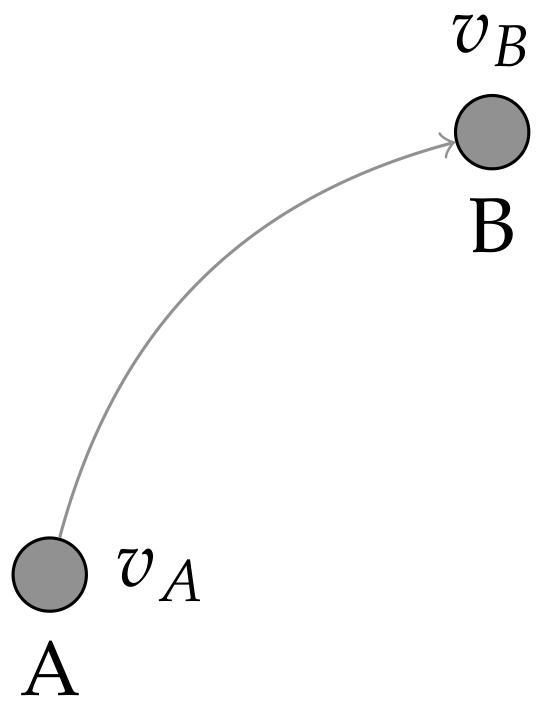
\includegraphics[width=0.2\linewidth]{../figs/tension_puntos.PNG}
		\caption{Diferencia de potencial}
		\label{fig.tension_puntos}
	\end{figure}
	
	Puesto que el potencial eléctrico es el trabajo electrostático por unidad de carga, la unidad del SI para $v(t)$ y $u_{AB}(t)$ es el \textbf{voltio} [V]:
	\begin{equation*}
		1\;V=\dfrac{1\;J}{1\;C}.
	\end{equation*}
	\begin{remark}
		La unidad [V] se escribe en mayúsculas en honor a Alessandro Volta, físico y químico italiano del siglo XVIII famoso por la invención y desarrollo de la pila eléctrica en 1799.
	\end{remark}
	Además, el campo eléctrico también es conservativo, por lo que la diferencia de potencial entre A y B \textbf{no depende de la trayectoria} seguida para realizar el desplazamiento, sino únicamente del potencial existente en cada uno de los puntos (Figura~\ref{fig.diagrama_tension}). Sin embargo, y pese a que la trayectoria no es relevante, siempre hay que tener en cuenta el \textbf{sentido del desplazamiento} (Figura~\ref{fig.sentido_tension}). Así, si el movimiento se produce desde B hasta A.
	\begin{equation*}
		u_{BA}(t) = v_B(t) - v_A(t) = - u_{AB}(t). 
	\end{equation*}
	\begin{figure}[H]
		\centering
		\subfloat[Trayectoria]{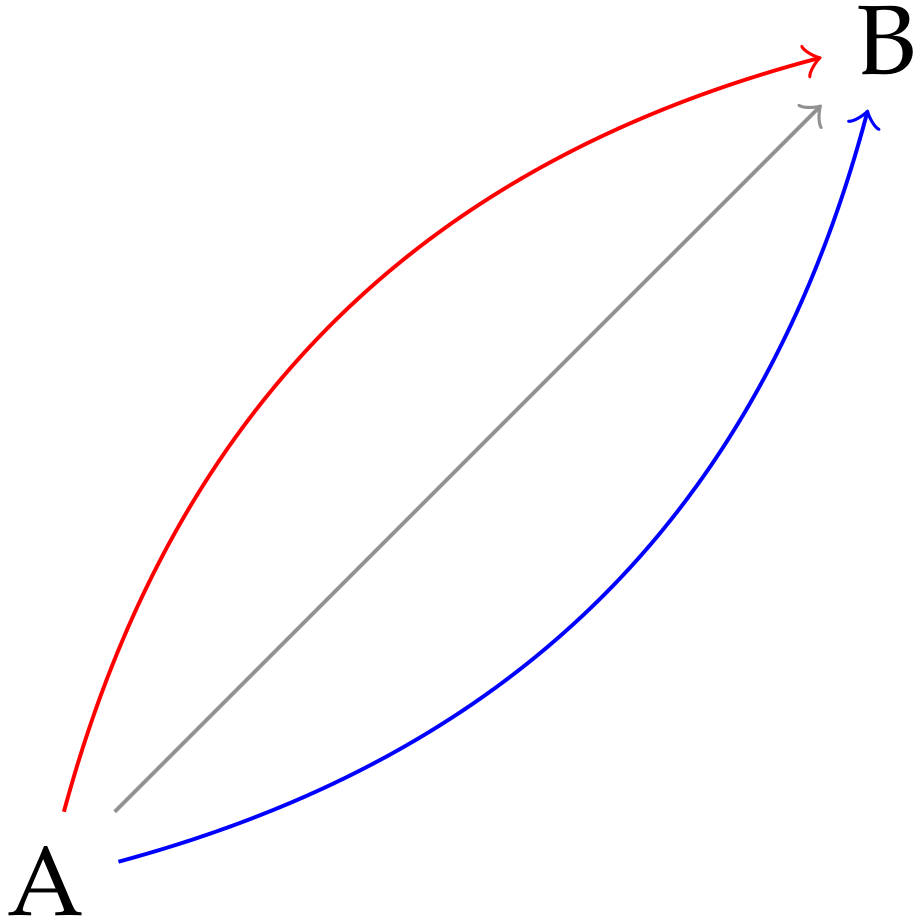
\includegraphics[width=0.25\linewidth]{../figs/diagrama_tension.PNG}\label{fig.diagrama_tension}}\hfil
		\subfloat[Sentido]{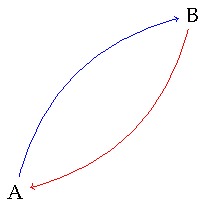
\includegraphics[width=0.25\linewidth]{../figs/sentido_tension.pdf}\label{fig.sentido_tension}}
		\caption{Consideraciones sobre la diferencia de potencial}
	\end{figure}
	
	\subsubsection{Corriente eléctrica}
	La \textbf{intensidad de la corriente eléctrica}, $i(t)$, se define como la variación de la carga eléctrica $q(t)$ que atraviesa la sección transversal de un conductor por unidad de tiempo (Figura~\ref{fig.seccion_conductor}). 
	\begin{equation*}\label{eq.intensidad}
		i(t)=\dfrac{dq(t)}{dt}
	\end{equation*}
	\begin{figure}[H]
		\centering
		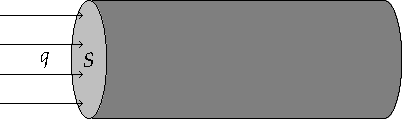
\includegraphics[width=0.45\linewidth]{../figs/seccion_conductor.pdf}
		\caption{Corriente eléctrica}
		\label{fig.seccion_conductor}
	\end{figure}
	
	La corriente eléctrica se produce por el \textbf{movimiento de los electrones libres} que fluyen por el conductor, es decir, que el \textbf{sentido real} de la intensidad es del polo $-$ al polo $+$ del generador (a través del conductor). Sin embargo, por razones históricas, el \textbf{convenio} que se emplea es justo el opuesto, esto es, del polo $+$ al polo $-$. La unidad en el SI de la corriente es el \textbf{amperio} [A]: 
	\begin{equation*}
		1\,A =\dfrac{1\,C}{1\,s}.
	\end{equation*}
	\begin{remark}
		La unidad [A] se escribe en mayúsculas en honor a André-Marie Ampère, matemático y físico francés del siglo XVIII-XIX, que inventó el primer telégrafo eléctrico y formuló la teoría del electromagnetismo en 1827.
	\end{remark}
	
	Cabe resaltar que el amperio es una unidad muy grande, por lo que a menudo se utilizan submúltiplos (mA, $\mu$A...). En algunos casos, puede hablarse también de la \textbf{densidad de corriente}, definida como el cociente entre la intensidad $i(t)$ y la sección transversal del conductor $S$:
	\begin{equation*}
		\delta =\dfrac{i(t)}{S}
	\end{equation*}
	La densidad de corriente se mide en el SI en [A/m$^2$], aunque en la industria suele venir determinada en [A/mm$^2$], al ser ésta una unidad más manejable.
	
	\subsubsection{Corriente continua y corriente alterna} \label{sec.cc-ca}
	Al estudiar la electricidad, es importante destacar que existen dos tipos de corriente: la corriente continua y la corriente alterna:
	\begin{itemize}
		\item \textbf{Corriente continua:} La corriente continua es aquella que siempre fluye en el mismo sentido (positivo o negativo). A su vez, puede ser:
		\begin{itemize}
			\item \textbf{Corriente continua constante:} Su valor instantáneo a lo largo del tiempo permanece inalterable ($\frac{di(t)}{dt} = 0$, Figura~\ref{fig.continua}). Suele estar suministrada por pilas, baterías, dinamos, fuentes de alimentación de corriente continua, etc. 
			\begin{figure}[H]
				\centering	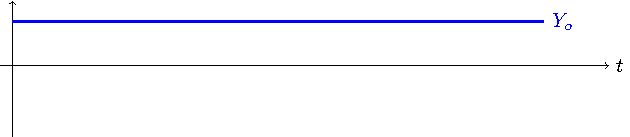
\includegraphics[width=0.75\linewidth]{../figs/continua.pdf}
				\caption{Forma de onda de la corriente continua constante}
				\label{fig.continua}
			\end{figure}
			\item \textbf{Corriente continua variable:} Su valor instantáneo no es constante a lo largo del tiempo, aunque siempre es del mismo signo (negativo o positivo). 
		\end{itemize}
		\item \textbf{Corriente alterna:} Aquella corriente que cambia de sentido (de positivo a negativo, y viceversa) cada cierto tiempo ($\frac{di(t)}{dt} \neq 0$). Se subdivide de nuevo en varios tipos:
		\begin{itemize}
			\item \textbf{Corriente alterna sinusoidal:} Los valores absolutos instantáneos son sucesivamente proporcionales a los valores que toma el seno de 0$^\circ$ a 360$^\circ$ (Figura~\ref{fig.sinBT1}).
			\begin{figure}[H]
				\centering
				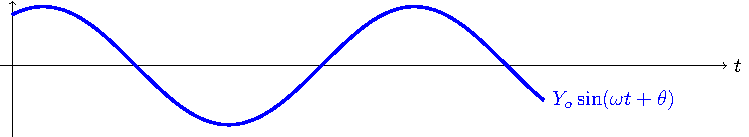
\includegraphics[width=0.75\linewidth]{../figs/sin.pdf}
				\caption{Forma de onda de la corriente alterna senoidal}
				\label{fig.sinBT1}
			\end{figure}
			\item \textbf{Corriente alterna periódica:} Tiene una forma de onda que se repite de manera periódica, cambiando de sentido, pero no es sucesivamente proporcional a los valores que toma el seno de 0$^\circ$ a 360$^\circ$.
			\item \textbf{Corriente alterna aperiódica:} Tiene una forma de onda que cambia de sentido pero sin seguir ningún periodo.
		\end{itemize}
	\end{itemize}
	Por comodidad, a la corriente continua constante se la conoce simplemente como \textit{corriente continua} (CC) y a la corriente alterna sinusoidal como \textit{corriente alterna} (CA).
	
	
	\subsubsection{Fuerza electromotriz (f.e.m.)}
	En todo circuito eléctrico es necesaria la existencia de al menos un elemento activo que suministre energía eléctrica, de manera que las cargas permanezcan en movimiento y, por tanto, exista corriente eléctrica. La causa capaz de mantener los electrones en movimiento en un circuito recibe el nombre de \textbf{fuerza electromotriz} (f.e.m.). Los dispositivos capaces de proporcionar esta diferencia de potencial estacionaria, permitiendo mantener una corriente eléctrica, son los \textbf{generadores} (baterías, pilas, dinamos, etc.), siendo la f.e.m. ($E$, $e(t)$ o $\epsilon$) la característica de éstos.  Por tanto, la fuerza electromotriz representa la energía que el generador cede a la unidad de carga eléctrica. Al tener la misma naturaleza que la tensión eléctrica, también se mide en voltios [V]. 
	
	\subsubsection{Potencia eléctrica}
	La \textbf{potencia eléctrica} es la variación del trabajo del campo eléctrico por unidad de tiempo:
	\begin{equation*}
		p(t)=\frac{dW_{e}}{dt} 
	\end{equation*}
	que puede relacionarse con las variables anteriores:
	\begin{equation*}\label{eq.pvi}
		p(t) = \frac{dW_e}{dq(t)} \cdot \frac{dq(t)}{dt}= u(t)\cdot i(t)
	\end{equation*}
	
	La {unidad} de la potencia eléctrica en el SI es el \textbf{vatio} [W]: 
	\begin{equation*}
		1\;W = \dfrac{1\;J}{1\;s}= 1\;A\cdot 1\;V.
	\end{equation*}
	\begin{remark}
		La unidad [W] se escribe en mayúsculas en honor a James Watt, ingeniero mecánico, inventor y químico escocés de los siglos XVIII-XIX, por sus contribuciones al desarrollo de la máquina de vapor, fundamental en el desarrollo de la primera Revolución Industrial.
	\end{remark}
	
	Para determinar el \textbf{signo de la potencia eléctrica} (Figura~\ref{fig.signo_potencia}) hay que tener en consideración los signos de las variables de las que depende (tensión y corriente): 
	\begin{itemize}
		\item Cuando las flechas de ambas variables tienen el \textbf{mismo sentido}, la potencia eléctrica es \textbf{positiva} ($P>0$)
		\item Cuando las flechas tienen \textbf{sentidos opuestos}, la potencia eléctrica es \textbf{negativa} ($P<0$)
	\end{itemize}
	\begin{figure}[H]
		\centering
		\subfloat[$P>0$]{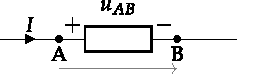
\includegraphics[width=0.3\linewidth]{../figs/signo_potencia1.pdf}}\hfil
		\subfloat[$P<0$]{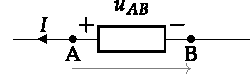
\includegraphics[width=0.3\linewidth]{../figs/signo_potencia2.pdf}}
		\caption{Convenio de signos para la potencia}
		\label{fig.signo_potencia}
	\end{figure}
	En la práctica, no es conveniente trabajar con potencias negativas, por lo que es habitual interpretar este resultado como potencia absorbida y potencia generada/entregada (Figura~\ref{fig.receptor_generador}):
	\begin{itemize}
		\item Un circuito o elemento es un \textbf{receptor} (absorbe potencia) cuando la corriente \emph{entra} por el terminal de mayor potencial
		\item Un circuito o elemento es un \textbf{generador} (entrega potencia) cuando la corriente \emph{sale} por el terminal de mayor potencial
	\end{itemize}
	\begin{figure}[H]
		\centering
		\subfloat[Receptor]{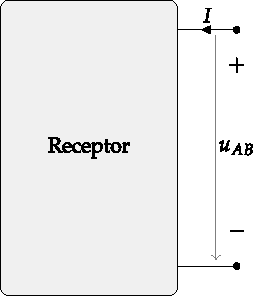
\includegraphics[width=0.25\linewidth]{../figs/receptor_generador1.pdf}}\hfil
		\subfloat[Generador]{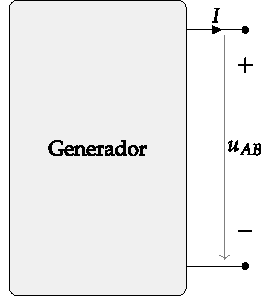
\includegraphics[width=0.25\linewidth]{../figs/receptor_generador2.pdf}}
		\caption{Convenio de signos para la potencia}
		\label{fig.receptor_generador}
	\end{figure}
	
	\begin{remark}
	    Téngase en cuenta, que por el principio de conservación de la energía, la potencia generada y la potencia consumida en un circuito deben ser iguales.
	\end{remark}
	
	\subsubsection{Energía y potencia}
	
	La \textbf{energía} $W$ es una magnitud física asociada con la capacidad que tienen los cuerpos para realizar un trabajo (emitir luz, generar calor, etc.). Puede manifestarse de distintas formas: gravitatoria, cinética, química, eléctrica, magnética, nuclear, radiante, etc., existiendo la posibilidad de transformar unos tipos de energía en otros, pero respetando siempre el principio de conservación de la energía. En el SI, la energía (del tipo que sea) se mide en julios [J]. El julio se define como el trabajo realizado por una fuerza $F$ de 1 Newton [N] cuando provoca un desplazamiento $d$ de 1 metro [m]. Por tanto, una forma de definir la energía es:
	\begin{equation*}
		W=F\cdot d 
	\end{equation*}
	\begin{remark}
		La unidad [J] se escribe en mayúsculas en honor a James Prescott Joule, físico e investigador inglés del siglo XIX, considerado como uno de los físicos más notables de su época. 
	\end{remark}
	
	Dado que la potencia $P$ se define como la cantidad de trabajo realizado (es decir, la energía $W$) por unidad de tiempo $t$ ($P=\frac{W}{t}$), también se puede definir la energía como:
	\begin{equation*}\label{eq.Ept}
		W=P\cdot t
	\end{equation*}
	Por tanto, otra unidad muy utilizada para medir energía es el vatio-hora [Wh], aunque ésta \textbf{\emph{no}} es la aceptada en el SI. Esta unidad representa el trabajo realizado por una máquina de potencia 1 W durante un tiempo de 1 hora. El Wh se utiliza comúnmente para medir la \textbf{energía eléctrica}. 
	
	\vspace{4mm}
	\begin{example}
		\textbf{¿Cuál es la equivalencia entre un kWh y un J?}
		\begin{equation*}
		    1 kWh = 1 kW \cdot 1 h = 1000 W \cdot 3600 s = 3.6 MJ 
		\end{equation*}
	\end{example}
	
	\section{Leyes básicas}
	
	\subsection{Ley de Ohm}
	
	La ley de Ohm, postulada por el físico  alemán Georg Ohm (1789--1854), es una ley que establece la relación entre la tensión y la intensidad de la corriente eléctrica, de acuerdo a la expresión: 
	\begin{equation}
	   \boxed{ U=R\cdot I}
	\end{equation}
    donde $R$ es la resistencia que opone el material al paso de la corriente eléctrica (se profundiza más en el concepto de \textbf{resistencia} en la Sección~\ref{sec.resistencia}).
	
	\subsection{Leyes de Kirchhoff}
	
	Existen una serie de definiciones previas que es necesario conocer para el análisis y la teoría de circuitos eléctricos:
	\begin{itemize}
		\item \textbf{Nudo:} unión de \textbf{3} o más conductores
		\item \textbf{Rama:} elementos conectados entre dos nudos consecutivos
		\item \textbf{Lazo:} conjunto de ramas que forman un camino cerrado
		\item \textbf{Malla:} lazo que no contiene ningún otro en su interior
	\end{itemize}

	\begin{example}\label{ej.1-3}
		\textbf{Determinar el número de nudos, ramas, lazos y mallas del circuito de la Figura~\ref{fig.mallas}.}
		\begin{figure}[H]
			\centering
			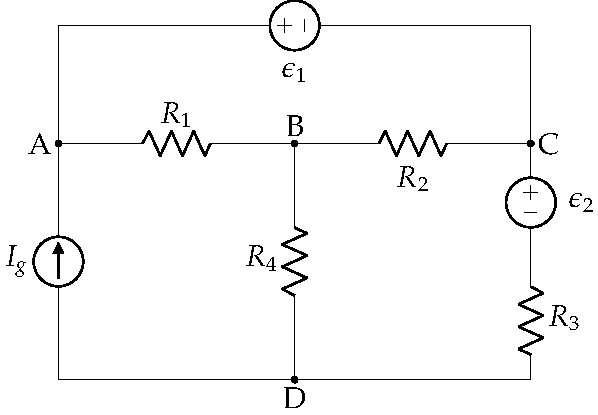
\includegraphics[width=0.5\linewidth]{../figs/mallas.pdf}
			\caption{Ejemplo~\ref{ej.1-3}}
			\label{fig.mallas}
		\end{figure}
		
		Nudos: 4 (A, B, C, D)
		
		Ramas: 6 (AB, AC, AD, BC, BD, DC)
		
		Lazos: 7 (ABDA, BCDB, ACBA, ABCDA, ACBDA, BDCAB, ACDA) 
		
		Mallas: 3 (ABDA, BCDB, ACBA)
	\end{example}
	
	
	Aún era un estudiante cuando en 1845 Gustav Robert Kirchhoff, a la edad de 21 años, realizó la primera de sus grandes aportaciones a la física, formulando las ahora denominadas \textbf{leyes de Kirchhoff}, ecuaciones básicas de los circuitos eléctricos.
	
	\begin{itemize}
		\item \textbf{Primera ley de Kirchhoff}. Esta ley es el resultado directo del \textbf{principio de conservación de la carga} aplicado a los circuitos eléctricos. Se conoce como primera ley de Kirchhoff (1LK) o ley de Kirchhoff de las corrientes (LKC), y dice que la suma algebráica de las intensidades de corriente que concurren en un nudo es cero. Esto es igual a decir que la suma de las corrientes que llegan a un nudo es igual a la suma de las que salen: 
		\begin{equation}
			\boxed{\sum_{i=1}^n i_i(t)=0}
		\end{equation}
		Así, en la Figura~\ref{fig.LKC_FM} se cumple que:
		\begin{equation*}
			i_1(t) - i_2(t) + i_3(t) - i_4(t) + i_5(t) = 0
		\end{equation*}
		
		\begin{figure}[H]
			\centering
			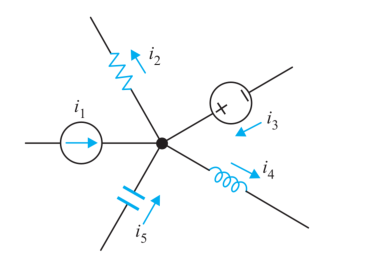
\includegraphics[width=0.35\linewidth]{../figs/LKC_FM.pdf}
			\caption{Primera ley de Kirchhoff}
			\label{fig.LKC_FM}
		\end{figure}
		\item \textbf{Segunda ley de Kirchhoff.} Esta ley es consecuencia del \textbf{principio de conservación de la energía} aplicado a los circuitos eléctricos. Se le
		denomina segunda ley de Kirchhoff (2LK) o ley de Kirchhoff de los voltajes (LKV), y dice que la suma (con signo) de las tensiones a lo largo de un circuito cerrado es cero. Esto quiere decir que la energía producida por un generador es consumida por los receptores del circuito
		para producir algún tipo trabajo (mecánico, químico, etc.) o calor:
		\begin{equation}
			\boxed{\sum_{j=1}^m u_i(t)=0}
		\end{equation}
		Así, en el circuito de la Figura~\ref{fig.LKV_FM}, se cumple que:
		\begin{equation*}
			u_3(t) + u_4 (t) - u_5 (t) - u_1 (t) - u_2 (t)  = 0 
		\end{equation*}
		\begin{figure}[H]
			\centering
			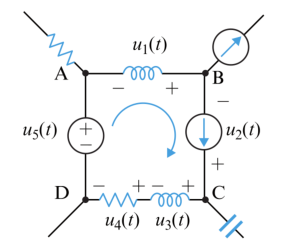
\includegraphics[width=0.35\linewidth]{../figs/LKV_FM.pdf}
			\caption{Segunda ley de Kirchhoff}
			\label{fig.LKV_FM}
		\end{figure}
	\end{itemize}
	
% 	\subsection{Balance de tensiones: ecuación de una rama y ley de Ohm para un circuito cerrado}
% 	\begin{figure}[H]
% 		\centering
% 		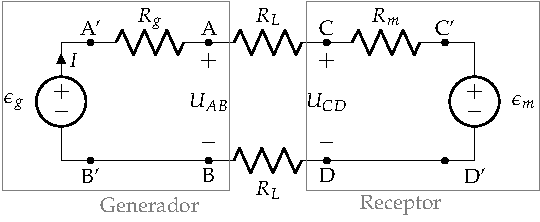
\includegraphics[width=0.5\linewidth]{../figs/circuito_lkv.pdf}
% 		\caption{Ecuación de una rama}
% 		\label{fig.circuito_lkv}
% 	\end{figure}
% 	Escribir la ecuación de una rama implica \textbf{determinar la diferencia de potencial que tiene aplicada}. Considérese el circuito de la Figura~\ref{fig.circuito_lkv}. Se cumple que, en las ramas $AB$ y $CD$: 
% 	\begin{equation*}
% 		U_{AB} = U_{AA'} + U_{A'B'} + U_{B'B}; \qquad
% 		U_{CD} = U_{CC'} + U_{C'D'} + U_{D'D}
% 	\end{equation*}
% 	y, aplicando la Ley de Ohm a cada resistencia:
% 	\begin{equation*}
% 		U_{A'A} = I \cdot R_g; \qquad
% 		U_{AC} = I \cdot R_L; \qquad 
% 		U_{CC'} = I \cdot R_m; \qquad
% 		U_{DB} = I \cdot R_L
% 	\end{equation*}
% 	Las tensiones $U_{D'D}= U_{BB'} = 0$, dado que no hay ningún elemento conectado entre ellos y, por tanto, no hay diferencia de potencial. Por último, en los generadores $\epsilon_g$ y $\epsilon_m$, se cumple que:
% 	\begin{equation*}
% 		U_{C'D'} = \epsilon_m;\qquad
% 		U_{B'A'} = -\epsilon_g
% 	\end{equation*}
% 	Por tanto: 
% 	\begin{equation*}
% 		U_{AB} = U_{AA'} + U_{A'B'} + \cancel{U_{B'B}}=-U_{A'A}-U_{A'B}=-I \cdot R_g-(-\epsilon_g)=\epsilon_g-I \cdot R_g% \rightarrow   {U_{AB} = \epsilon_g - I \cdot R_g}
% 	\end{equation*}
	
% 	\begin{equation*}
% 		U_{CD} = U_{CC'} + U_{C'D'} + \cancel{U_{D'D}}=I \cdot R_m +\varepsilon_m%\rightarrow {U_{CD} = \epsilon_m + I\cdot R_m}
% 	\end{equation*}
% 	En general, puede decirse que la diferencia de potencial de una rama es igual al producto de la intensidad que circula por ella por la suma de todas las resistencias que contiene, menos la suma algebraica de todas la
% 	fuerzas electromotrices, consideradas positivas ($+$) las que tienden a crear corriente en el sentido que se recorre la rama y negativas ($-$) en caso contrario:
% 	\begin{equation}\label{eq.ecuacion_rama}
% 		\boxed{U=I\cdot \sum_{i=1}^n R_i-\sum_{j=1}^m \varepsilon_j}
% 	\end{equation}
	
% 	Considerando ahora el circuito cerrado, tal como se muestra en la Figura~\ref{fig.circuito_lkv}, aplicando la 2LK: 
% 	\begin{equation*}
% 		U_{A'A} + U_{AC} + U_{CC'} + U_{C'D'} + \cancel{U_{D'D}} + U_{DB} + \cancel{U_{BB'}} + U_{B'A'} = I \cdot R_g+I \cdot R_L+I \cdot R_m+\epsilon_m+I \cdot R_L-\epsilon_g=0
% 	\end{equation*}
% 	Por tanto, despejando la $I$ de la expresión anterior, se llega a:
% 	\begin{equation*}
% 		I=\dfrac{\epsilon_g-\epsilon_m}{R_g + 2\cdot R_L + R_m}
% 	\end{equation*}
% 	Generalizando esta ecuación, se obtiene la conocida Ley de Ohm para un circuito cerrado, considerando las f.e.m. positivas ($+$) si tienden a crear corriente en el sentido que se recorre la malla, y negativas ($-$) en caso contrario:
% 	\begin{equation}
% 		\boxed{I=\dfrac{\displaystyle\sum_{j=1}^m \varepsilon_j}{\displaystyle\sum_{i=1}^n R_i}}
% 	\end{equation}
	
	\section{Elementos de los circuitos}
	Como ya se mencionó en la Sección~\ref{sec.circuito_electrico}, en un circuito eléctrico existen dos tipos de elementos: los elementos activos y los pasivos.
	
	\subsection{Elementos activos}\label{sec.elementos_activos}
	
	\subsubsection{Generadores de tensión}
	Un \textbf{generador de tensión} es un dispositivo físico, caracterizado por una fuerza electromotriz $\epsilon$ que proporciona una diferencia de potencial $U$ entre sus bornes de salida. Por tanto, \textbf{impone la tensión} a su salida, mientras que \emph{la corriente depende del circuito} (Figura~\ref{fig.fuentetension}).
	\begin{itemize}
		\item Un \textbf{generador ideal} es aquel que \textbf{no tiene pérdidas}, de tal forma que la diferencia de potencial entre sus bornes toma siempre el mismo valor que su f.e.m. ($u_{AB}=\epsilon_g$). Además, se dice que un generador de tensión ideal es \textbf{dominante} sobre todo lo que está conectado en paralelo con él, ya que impone entre sus terminales la tensión que lo caracteriza. Así, a efectos de cálculo, puede prescindirse de las ramas que no interese estudiar.
		\item Un \textbf{generador real} es aquel que \textbf{tiene pérdidas}, caracterizadas mediante una resistencia interna, en \textbf{serie}, $R_{\epsilon_g}$. Al circular una corriente por dicha resistencia, se consume en ella una potencia que no puede ser entregada por el generador. Las pérdidas internas son la causa de que la diferencia de potencial entre sus bornes sea inferior a la f.e.m. ($u_{AB}<\epsilon_g$). Con esto, la potencia generada será $P_g=\epsilon_g\cdot I$, la potencia disipada en la resistencia interna $P_p=R_{\epsilon_g}\cdot I^2$ y la potencia útil $P_u=U_{AB}\cdot I$ y, dado que tiene que cumplirse el principio de conservación de la energía:
		\begin{equation}
			P_g=P_u+P_p\rightarrow \boxed{ \epsilon_g=U_{AB}+ R_{\epsilon_g}\cdot I}
		\end{equation}
	\end{itemize}
	\begin{figure}[H]
		\centering
		\subfloat[Ideal]{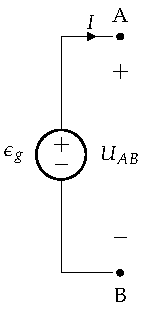
\includegraphics[height=3.5cm]{../figs/FuenteTensionIdealDC.pdf}}\hfil
		\subfloat[Real]{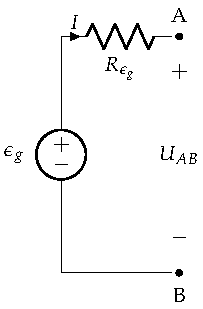
\includegraphics[height=3.5cm]{../figs/FuenteTensionRealDC.pdf}}
		\caption{Generador de tensión}
		\label{fig.fuentetension}
	\end{figure}
	
	\subsubsection{Generadores de corriente}
	Un \textbf{generador de corriente} es un dispositivo físico, caracterizado por una intensidad $I_g$ que proporciona una corriente $I$. Por tanto, \textbf{impone la corriente} a su salida, mientras que \emph{la tensión depende del circuito} (Figura~\ref{fig.fuentecorriente}).
	\begin{itemize}
		\item Un \textbf{generador ideal} es aquel que \textbf{no tiene pérdidas}, de tal forma que la corriente $I$ a su salida toma siempre el mismo valor que $I_g$ ($I=I_g$). Un generador de intensidad ideal es \textbf{dominante} sobre todo lo que está conectado en serie con él ya que impone en esa rama la corriente que lo caracteriza. A efectos de cálculo, puede prescindirse de los elementos en serie que no interese estudiar. 
		\item Un \textbf{generador real} es aquel que \textbf{tiene pérdidas}, caracterizadas mediante una resistencia interna, en \textbf{paralelo}, $R_{I_g}$. Al producirse una derivación de corriente por esa resistencia, circular una corriente por dicha resistencia, se consume en ella una potencia que no puede ser entregada por el generador. Las pérdidas internas son la causa de que la corriente suministrada sea menor a la que caracteriza al generador ($I<I_g$). Con esto, la potencia generada será $P_g=U_{AB}\cdot I_g$, la potencia disipada en la resistencia interna $P_p=\frac{U_{AB}^2}{R_{I_g}}$ y la potencia útil $P_u=U_{AB}\cdot I$ y, dado que tiene que cumplirse el principio de conservación de la energía:
		\begin{equation}
			P_g=P_u+P_p\rightarrow \boxed{I_g=I+ \dfrac{U_{AB}}{R_{I_g}}}
		\end{equation}
	\end{itemize}
	\begin{figure}[H]
		\centering
		\subfloat[Ideal]{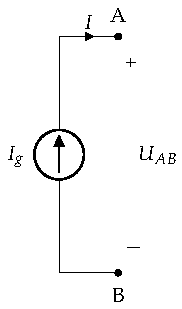
\includegraphics[height=3.5cm]{../figs/FuenteCorrienteIdeal.pdf}}\hfil
		\subfloat[Real]{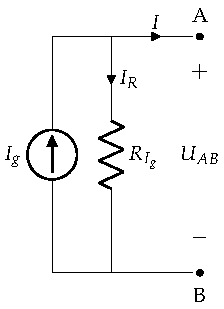
\includegraphics[height=3.5cm]{../figs/FuenteCorrienteRealDC.pdf}}
		\caption{Generador de corriente}
		\label{fig.fuentecorriente}
	\end{figure}
	
	\subsubsection{Dualidad de generadores}\label{sec.dualidad}
	
	Se dice que dos fuentes son equivalentes cuando suministran el \textbf{mismo valor de tensión y corriente} a un circuito externo, para cualquier circuito. Esta equivalencia solo puede darse entre \textbf{fuentes reales}.
	
	\begin{figure}[H]
		\centering
		\subfloat[Fuente real de tensión]{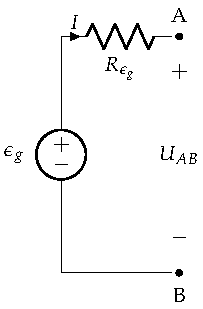
\includegraphics[height=4.9cm]{../figs/FuenteTensionRealDC.pdf}}\hfil
		\subfloat[Fuente real de corriente]{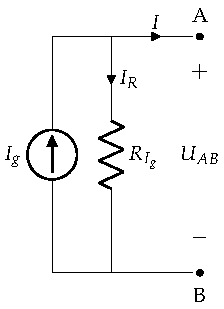
\includegraphics[height=4.9cm]{../figs/FuenteCorrienteRealDC.pdf}}
		\caption{Equivalencia de generadores}
		\label{fig.equivalencia_generadores}
	\end{figure}
	
	Considérense las fuentes de tensión y corriente, reales, mostradas en la Figura~\ref{fig.equivalencia_generadores}
	La salida de la fuente de tensión es:
	\begin{equation*}
		U_{AB} = \epsilon_g - R_{\epsilon_g} \cdot I
	\end{equation*}
	y la de la fuente de corriente:
	\begin{equation*}
		I = I_g - \frac{U_{AB}}{R_{I_g}} \rightarrow U_{AB} = R_{I_g} \cdot I_g - R_{I_g} \cdot I
	\end{equation*} 
	Por tanto, las fuentes son equivalentes cuando las ecuaciones coinciden para cualquier combinación de $(U_{AB}, I)$, es decir, si $R_g = R_{\epsilon_g} = R_{I_g}$:
	\begin{equation}\label{eq.equivalencia_fuentes}
		\boxed{\epsilon_g = R_{\epsilon_g} \cdot I_g \Leftrightarrow {I_g = \frac{\epsilon_g}{R_g}}}  
	\end{equation}
	
	\begin{remark}
	    Nótese que el polo $+$ de la fuente de tensión queda en la misma posición que la flecha de la fuente de corriente
	\end{remark}
	
	\begin{example}\label{ex.1-2}
	    \textbf{Convertir en fuente de intensidad o de tensión, según corresponda, las fuentes mostradas en la Figura~\ref{fig.ejemplo1-2}.}
	    \begin{figure}[H]
	        \centering
	        \subfloat[]{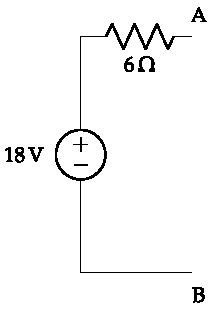
\includegraphics[height=3.5cm]{../figs/Conversion_Fuentes.pdf}}\hfil
	        \subfloat[]{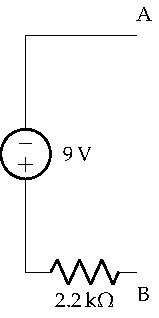
\includegraphics[height=3.5cm]{../figs/Conversion_Fuentes_2.pdf}}\hfil
	        \subfloat[]{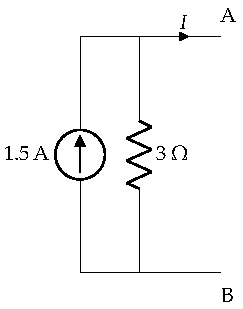
\includegraphics[height=3.5cm]{../figs/Conversion_Fuentes_3.pdf}}\hfil
	        \subfloat[]{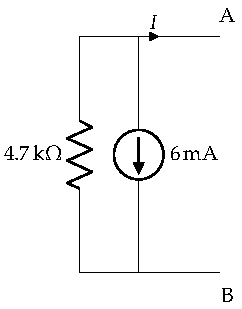
\includegraphics[height=3.5cm]{../figs/Conversion_Fuentes_4.pdf}}
	        \caption{Ejemplo~\ref{ex.1-2}}
	        \label{fig.ejemplo1-2}
	    \end{figure}
	    
	    \textbf{GENERADOR (a)}
	    
	    Se puede transformar en un generador de corriente con una resistencia en paralelo de $6\Omega$, y de intensidad de la fuente $I_g=\frac{18}{6}=3$ A, con la punta de flecha hacia arriba.
	    
	    \textbf{GENERADOR (b)}
	    
	    Se puede transformar en un generador de corriente con una resistencia en paralelo de $2.2k\Omega$, y de intensidad de la fuente $I_g=\frac{9}{2.2\cdot10^3}=4.1$ mA, con la punta de flecha hacia abajo.
	    
	    \textbf{GENERADOR (c)}
	    
	    Se puede transformar en un generador de tensión con una resistencia en serie de $3\Omega$, y de fem de la fuente $\varepsilon_g=1.5\cdot 3=4.5$ V, con el polo $+$ arriba.
	    
	    \textbf{GENERADOR (d)}
	    
	    Se puede transformar en un generador de tensión con una resistencia en serie de $4.7k\Omega$, y de fem de la fuente $\varepsilon_g=6\cdot 10^{-3}\cdot 4.7\cdot 10^3=28.2$ V, con el polo $+$ abajo.
	\end{example}
	
	\subsubsection{Generadores dependientes o generadores controlados}
	Pese a no ser estrictamente elementos activos, se comportan como tales. Este tipo de generadores no tienen valores de $\epsilon$ o $i_g$ fijos, sino que dependen de la tensión o corriente en otros puntos de la red. Así, aparecen fundamentalmente cuatro tipos de generadores dependientes, dependiendo de que cada generador suministre una tensión o una corriente y según sea la variable de control una tensión o una corriente. Estos generadores suelen representarse mediante un rombo:
	\begin{itemize}
		\item \textbf{Generador de tensión controlado por tensión} (Figura~\ref{fig.tension-tension}): su tensión depende de la tensión entre otros puntos del circuito, siendo el parámetro $\alpha$ adimensional [--]
		\item \textbf{Generador de tensión controlado por corriente} (Figura~\ref{fig.tension-corriente}): su tensión depende de alguna corriente del circuito, teniendo el parámetro $\beta$ unidades de resistencia [$\Omega$]
		\item \textbf{Generador de corriente controlado por tensión} (Figura~\ref{fig.corriente-tension}): su intensidad depende de la tensión entre dos puntos del circuito, teniendo el parámetro $\gamma$ unidades de conductancia [S]
		\item \textbf{Generador de corriente controlado por corriente} (Figura~\ref{fig.corriente-corriente}): su intensidad es función de la corriente en otra parte del circuito, siendo el parámetro $\sigma$ adimensional [--]
	\end{itemize}
	\begin{figure}[H]
		\centering
		\subfloat[Tensión--Tensión]{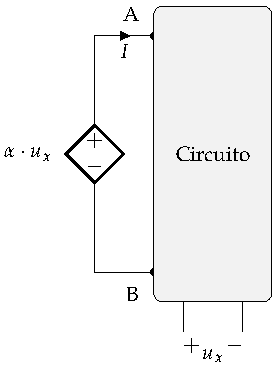
\includegraphics[height=4cm]{../figs/FuenteTensionDependienteTension.pdf}\label{fig.tension-tension}}\hfill
		\subfloat[Tensión--Corriente]{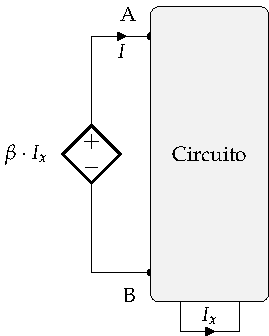
\includegraphics[height=4cm]{../figs/FuenteTensionDependienteCorriente.pdf}\label{fig.tension-corriente}}\hfill
		\subfloat[Corriente--Tensión]{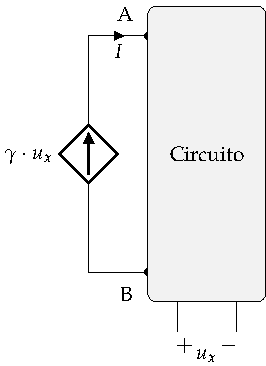
\includegraphics[height=4cm]{../figs/FuenteCorrienteDependienteTension.pdf}\label{fig.corriente-tension}}\hfill
		\subfloat[Corriente--Corriente]{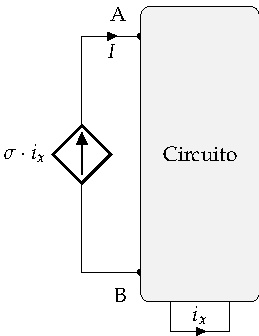
\includegraphics[height=4cm]{../figs/FuenteCorrienteDependienteCorriente.pdf}\label{fig.corriente-corriente}}
		\caption{Fuentes dependientes}
		\label{fig.fuentes_dependientes}
	\end{figure}
	
	\begin{remark}
		Si en un circuito \textbf{solo} existen generadores dependientes, el circuito \textbf{no está excitado}.
	\end{remark} 
	
	
	
	
	
%	\subsection{Elementos pasivos}\label{sec.elementos_pasivos}
	
	% Los receptores son todos aquellos dispositivos capaces de transformar la energía eléctrica en otra forma de energía (por ejemplo, un motor transforma la energía eléctrica en energía mecánica). Se caracterizan por su fuerza contraelectromotriz
	% (f.c.e.m., $E'$ o $e'(t)$), que es la energía por unidad de carga que transforman
	% en otro tipo de energía (siempre que ésta no sea calor). Por su definición, la unidad en el SI es también el \textbf{voltio} [V].
	
	\subsection{Elementos pasivos ideales}
	
	En general, en teoría de circuitos se emplean tres tipos de elementos pasivos: resistencias, bobinas y condensadores. Se dice que un receptor es cualquier dispositivo capaz de transformar la energía eléctrica en otra forma de energía (que no sea solo calor); así, un ejemplo de receptor es un motor eléctrico (transforma parte de la energía eléctrica en mecánica).  
	
	\subsubsection{Resistencia} \label{sec.resistencia}
	En el siglo XIX, Georg Simon Ohm descubrió la ley que lleva su nombre (\textbf{ley de Ohm}). Dicha ley obtiene que, \textit{a temperatura constante}, la relación existente entre la diferencia de potencial entre los bornes de un conductor y la intensidad de corriente que circula por él es una constante, denominada \textbf{resistencia eléctrica}:
	\begin{equation*}
		\boxed{u(t)=R\cdot i(t)}
	\end{equation*}
	Por tanto, la resistencia eléctrica representa la mayor o menor dificultad que ofrecen los diferentes materiales para ser recorridos por una corriente eléctrica. Su valor se mide en ohmios [$\Omega$]. El criterio de signos utilizado considerar que la tensión es positiva en el terminal por el que entra la corriente, esto es, las flechas de tensión y corriente tienen el mismo sentido (Figura~\ref{fig.resistencia}).
	\begin{figure}[H]
		\centering
		\subfloat[Referencia mediante signo]{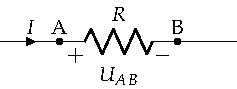
\includegraphics{../figs/Resistencia.pdf}}\hfil
		\subfloat[Referencia mediante flecha]{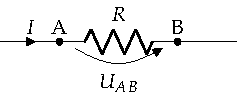
\includegraphics{../figs/Resistencia_Flecha.pdf}}
		\caption{Criterio de signos en una resistencia}
		\label{fig.resistencia}
	\end{figure}
	
	La magnitud que determina si un material es mejor o peor conductor se denomina \textbf{resistividad} ($\rho$), medida en [$\Omega\cdot$m] en el SI, aunque en las aplicaciones prácticas se suele utilizar el [$\Omega\cdot$m$^2/m$]. La resistividad de un material permanece constante si no varía la temperatura (suele expresarse a 20$^\circ$C). Para conductores homogéneos, de sección constante y pequeña comparada con su longitud, la resistencia $R$ que ofrece al paso de la corriente se puede determinar a partir de: 
	\begin{equation*}\label{eq.resistencia_rho}
		R=\rho\cdot \dfrac{l}{S}
	\end{equation*}
	siendo $l$ la longitud del conductor y $S$ el área de la sección transversal del mismo. Cabe destacar, por su importancia en la industria, la resistividad del cobre ($\rho_{Cu}=1/58\;\Omega \cdot$mm$^2/$m) y la del aluminio ($\rho_{Al}=1/36\;\Omega \cdot$mm$^2/$m).
	
	\vspace{4mm}
	\begin{example}
		\textbf{Calcular la resistencia de un conductor de cobre que tiene una longitud $l=10$~m y una sección $S=2$~mm$^2$.}\\
		Aplicando la expresión anterior: 
		\begin{equation*}
			R=\rho\cdot \dfrac{l}{S}=(1/58)\cdot \dfrac{10}{2}=0.086\;\Omega
		\end{equation*}
	\end{example}
	
	Para temperaturas distintas de 20$^\circ$C, siempre que la temperatura final $T_f$ esté en torno a los 250$^\circ$, la resistividad y, por tanto, la resistencia pueden determinarse a partir de las siguientes expresiones:
	\begin{equation*}
		\rho_f=\rho_{20}\cdot (1+\alpha\cdot (T_f-20)); \qquad
		R_f=R_{20}\cdot (1+\alpha\cdot (T_f-20))
	\end{equation*}
	donde $\rho_f$ y $R_f$ son la resistividad y la resistencia a la temperatura $T_f$ (respectivamente), $\rho_{20}$ y $R_{20}$ son la resistividad y la resistencia a 20$^\circ$C (respectivamente) y $\alpha$ es el coeficiente de temperatura. 
	
	La inversa de la resistencia se denomina \textbf{conductancia}, $G$, y se mide en el SI en \textbf{Siemens} [S]. Al ser lo opuesto de la resistencia, representa la facilidad de los conductores al paso de la corriente eléctrica:
	\begin{equation}
		\boxed{G=\dfrac{1}{R}}
	\end{equation}
	\begin{remark}
		La unidad [S] se escribe en mayúsculas en honor a Ernst Werner M. von Siemens, inventor alemán del siglo XIX, pionero de la electrotecnia y fundador de la actual empresa Siemens.
	\end{remark}
	Asimismo, a la inversa de la resistividad se le denomina \textbf{conductividad} ($\gamma$), definida como la facilidad que ofrecen los materiales al paso de la corriente eléctrica, por unidad de longitud y sección:
	\begin{equation*}
		\gamma=\dfrac{1}{\rho}
	\end{equation*}
	
	El desplazamiento de cargas a través de los conductores produce interacciones y choques entre ellas que, a su vez, dan
	origen a un calentamiento del conductor. El físico británico James Prescott Joule, en 1841, fue quién cuantificó el valor del calor que se produce en un conductor por el paso de la corriente y enunció la ley que lleva su nombre (\textbf{ley de Joule}): toda la energía que absorbe un conductor homogéneo por el que circula una corriente eléctrica y en el que no existen f.e.m., se transforma íntegramente en calor. Por tanto, la energía ``perdida'' en forma de calor:
	\begin{equation*}
		W=P\cdot t=U\cdot I\cdot t=R\cdot I^2\cdot t
	\end{equation*}
	cuyo resultado viene expresado en [J]. Sin embargo, una unidad muy utilizada para medir el calor es la \textbf{caloría} [cal], cuya equivalencia con el [J] es:
	\begin{equation*}
		1\;J=0.24\;cal
	\end{equation*}
	En general, se dirá que una resistencia disipa energía eléctrica produciendo calor, siendo la potencia disipada: 
	\begin{equation*}
		p(t)=R\cdot i^{2}(t)
	\end{equation*}
	
	El concepto de resistencia se utiliza también para definir dos términos muy comunes en teoría de circuitos:
	\begin{itemize}
		\item \textbf{Cortocircuito:} Conductor ideal que se une entre dos puntos, haciendo de este modo que su resistencia sea $R=0\;\Omega$. El cortocircuito puede llevar cualquier corriente, cuyo valor depende del resto del circuito, pero la tensión entre sus terminales (por la ley de Ohm) es de $u_{AB}(t)=0$~V (Figura~\ref{fig.cortocircuito}). 
		\item \textbf{Circuito abierto:} Representa una ruptura del circuito en ese punto, por lo que no puede circular corriente ($i(t)=0$). Se puede considerar como un circuito con resistencia infinita ($R\rightarrow\infty$) y que puede tener cualquier tensión, que depende del resto de la red (Figura~\ref{fig.c_abierto}).
	\end{itemize}
	\begin{figure}[H]
		\centering
		\subfloat[Cortocircuito]{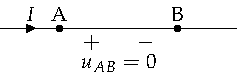
\includegraphics[width=0.25\linewidth]{../figs/cortocircuito.pdf}\label{fig.cortocircuito}}\hfil
		\subfloat[Circuito abierto]{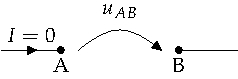
\includegraphics[width=0.25\linewidth]{../figs/CircuitoAbierto.pdf}\label{fig.c_abierto}}
		\caption{Cortocircuito y circuito abierto}
		
	\end{figure}
	
	\subsubsection{Bobina}\label{sec.bobina}
	
	Una \textbf{bobina} es un conductor arrollado, con $N$ vueltas, alrededor de un núcleo (generalmente, de material ferromagnético). La tensión en bornes de la bobina es directamente proporcional a la variación de la corriente respecto al tiempo, con un factor de proporcionalidad $L$ conocido como \textbf{inductancia} o coeficiente de autoinducción, medido en \textbf{henrios} [H] (Figura~\ref{fig.bobina}):
	\begin{equation}\label{eq.u_L}
		\boxed{u(t)=L\cdot\frac{di(t)}{dt}}\,
	\end{equation}
	por lo que, en circuitos de corriente continua, una bobina se comporta como un \textbf{cortocircuito}:
	\begin{equation*}
		\dfrac{di(t)}{dt} = 0 \rightarrow u = 0
	\end{equation*}
	\begin{remark}
		La unidad [H] se escribe en mayúsculas en honor a Joseph Henry, físico estadounidense del siglo XIX conocido por su trabajo acerca del electromagnetismo, electroimanes y relés.
	\end{remark}
	\begin{figure}[H]
		\centering
		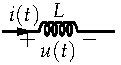
\includegraphics[width=0.15\linewidth]{../figs/Bobina.pdf}
		\caption{Tensión y corriente en una bobina}
		\label{fig.bobina}
	\end{figure}
	
	La relación inversa de la expresión~\eqref{eq.u_L} se puede obtener por integración entre un tiempo inicial $t_i$ y un tiempo final $t_f$, resultando:
	\begin{equation*}
		\int_{t_i}^{t_f} \dfrac{di(t)}{dt}dt=\dfrac{1}{L}\int_{t_i}^{t_f}u(t)\cdot dt \rightarrow i(t_f)-i(t_i)=\dfrac{1}{L}\cdot\int_{t_i}^{t_f} u(t)\cdot dt\,
	\end{equation*}
	\begin{equation}
		\boxed{i(t_f)=i(t_i)+\dfrac{1}{L}\cdot\int_{t_i}^{t_f} u(t)\cdot dt}
	\end{equation}
	Se observa que la bobina tiene un efecto de ``memoria'', ya que la corriente en un tiempo $t_f$ no depende solamente de la entrada $i(t)$ en ese momento, sino también del valor inicial de la entrada. Además, para establecer un flujo en una bobina, es necesario una energía de entrada, que queda almacenada después en forma de \textbf{campo magnético}. La potencia ``absorbida'' por la bobina será:
	\begin{equation*}
		p(t)=u(t)\cdot i(t)=L\cdot i(t)\cdot\dfrac{di(t)}{dt}
	\end{equation*}
	y la energía almacenada $w(t)$ en un periodo de tiempo entre $t_i$ y $t_f$ valdrá:
	\begin{equation*}
		w(t)=\int_{t_i}^{t_f}v(t)\cdot i(t)\cdot dt=\int_{t_i}^{t_f}L\cdot\dfrac{di(t)}{dt}\cdot i(t)\cdot dt=\dfrac{1}{2}\cdot L\cdot [i(t_f)-i(t_i)]^2
	\end{equation*}
	\begin{equation}
		\boxed{w(t)=\dfrac{1}{2}\cdot L\cdot [i(t_f)-i(t_i)]^2}
	\end{equation}
	
	\begin{remark}
	    Para entender el concepto de inductancia, es necesario recordar algunos principios del electromagnetismo. 
	\begin{itemize}
		\item \textbf{Ley de Ampère.} Es la ley fundamental que relaciona corrientes eléctricas y campos magnéticos. Su versión más simple dice que el producto de $N$ veces una corriente $i$ da lugar a una intensidad de campo magnético $H$ proporcional a la longitud magnética media de las líneas de dicho campo $l$:
		\begin{equation*}
			\label{eq.ampere_mod}
			H\cdot l=N\cdot i
		\end{equation*}
		\item \textbf{Densidad de flujo magnético.} La intensidad de campo $H$ origina, allá donde exista, una densidad de flujo $B$, cuyo valor es:
		\begin{equation*}\label{eq.B}
			B=\mu\cdot H,
		\end{equation*}
		siendo $\mu$ la permeabilidad del material. 
		\item \textbf{Flujo magnético.} Un campo magnético $B$ (constante en magnitud y dirección) que atraviesa un área $S$, formando un ángulo $\theta$ con ésta, crea un flujo magnético que se puede calcular como: 
		\begin{equation*}\label{eq.flujo1}
			\phi=B\cdot S\cdot \cos (\theta)
		\end{equation*}
		\item \textbf{Ley de Lenz-Faraday.} Un flujo magnético variable en el tiempo induce una fuerza electro-motriz (fem, $e$) que es igual en magnitud a la variación por unidad de tiempo del flujo inducido en el circuito. Esta fem inducida tiene un sentido tal que sus efectos tienden a oponerse a las causas que lo producen, por lo que: 
		\begin{equation*}\label{eq.lenz-faraday}
			e=-\dfrac{d\phi(t)}{dt}.
		\end{equation*}
	\end{itemize}
	A partir de esto, y con la ecuación~\eqref{eq.u_L}, es sencillo concluir que, cuando un circuito está formado únicamente por una bobina alimentada con una intensidad variable (es decir, corriente alterna) el flujo magnético también cambia y, por tanto, se induce una $fem$:
	\begin{equation*}
		e=\dfrac{d\phi(t)}{dt}=L\cdot \dfrac{di(t)}{dt} 
	\end{equation*}
	es decir, la $fem$ inducida es proporcional a la variación con el tiempo de la intensidad de corriente. Considerando esta expresión y despejando el valor de $L$, se tiene que: 
	\begin{equation*}
		L= \dfrac{d\phi(t)}{\cancel{dt}}\cdot\dfrac{\cancel{dt}}{di(t)}=\dfrac{d\phi(t)}{di(t)}
	\end{equation*}
	por lo que la inductancia $L$ expresa la relación entre el cambio de flujo y el cambio de corriente. 
	\end{remark}
	
	
	\subsubsection{Condensador}\label{sec.condensador}
	
	Un sistema de dos placas metálicas separadas por una capa dieléctrica constituye un \textbf{condensador}. Al aplicar tensión, produciendo una \textbf{separación de cargas opuestas} que se \textbf{acumulan} en cada placa (una de las placas queda con la carga $+Q$ y la otra con $-Q$). Del mismo modo que un elemento resistivo se distingue por el valor de su resistencia $R$, y una bobina por el valor de su inductancia $L$, un condensador se caracteriza por su \textbf{capacidad} $C$, que es la aptitud que tiene para acumular carga eléctrica. Así, la capacidad es la relación entre la carga $q(t)$ acumulada y la diferencia de potencial aplicada entre ellas $u(t)$, siendo:
	\begin{equation}\label{eq.cqu}
		\boxed{C=\dfrac{q(t)}{u(t)}}
	\end{equation}
	La unidad en el SI de la capacidad es el faradio [F]. Se trata de una unidad tremendamente grande, por lo que en la práctica se utilizan submúltiplos (mF, $\mu$F, pF...). 
	\begin{remark}
		La unidad [F] se escribe en mayúsculas en honor a Michael Faraday, científico británico de los siglos XVIII-XIX que estudió el electromagnetismo y la electroquímica. 
	\end{remark}
	
	Durante la carga del condensador, se produce una corriente eléctrica entre las dos placas (Figura~\ref{fig.condensador}): 
	\begin{equation}\label{eq.icu}
		i(t)=\dfrac{dq(t)}{dt}\stackrel{\eqref{eq.cqu}}{=}\dfrac{d(C\cdot u(t))}{dt}=C\cdot \dfrac{du(t)}{dt} \Rightarrow \boxed{i(t)=C\cdot \dfrac{du(t)}{dt}}
	\end{equation}
	por lo que, en circuitos de corriente continua, un condensador se comporta como un \textbf{circuito abierto}.
	\begin{equation*}
		\frac{du(t)}{dt} = 0 \rightarrow i = 0
	\end{equation*}
	\begin{figure}[H]
		\centering
		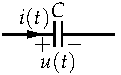
\includegraphics[width=0.15\linewidth]{../figs/Condensador.pdf}
		\caption{Tensión y corriente en un condensador}
		\label{fig.condensador}
	\end{figure}
	
	La relación inversa de la expresión~\eqref{eq.icu} se puede obtener por integración entre un tiempo inicial $t_i$ y un tiempo final $t_f$, resultando:
	\begin{equation*}
		\int_{t_i}^{t_f} \dfrac{du(t)}{dt}dt=\dfrac{1}{C}\int_{t_i}^{t_f}i(t)\cdot dt \rightarrow u(t_f)-u(t_i)=\dfrac{1}{C}\cdot\int_{t_i}^{t_f} i(t)\cdot dt
	\end{equation*}
	\begin{equation}\label{eq.u_C}
		\boxed{u(t_f)=u(t_i)+\dfrac{1}{C}\cdot\int_{t_i}^{t_f} i(t)\cdot dt}
	\end{equation}
	Se observa que el condensador también tiene un efecto de ``memoria'', ya que la tensión en un tiempo $t_f$ no depende solamente de la entrada $u(t)$ en ese momento, sino también del valor inicial.
	
	Al aplicar tensión a un condensador se produce una separación de cargas entre ambas placas, lo que produce un \textbf{campo eléctrico}, quedando almacenada una energía de este tipo. La potencia ``absorbida'' por el condensador será:
	\begin{equation*}
		p(t)=u(t)\cdot i(t)=C\cdot u(t)\cdot\dfrac{du(t)}{dt}
	\end{equation*}
	y la energía almacenada $w(t)$ en un periodo de tiempo entre $t_i$ y $t_f$ valdrá:
	\begin{equation*}
		w(t)=\int_{t_i}^{t_f}v(t)\cdot i(t)\cdot dt=\int_{t_i}^{t_f}C\cdot\dfrac{du(t)}{dt}\cdot u(t)\cdot dt=\dfrac{1}{2}\cdot C\cdot [u(t_f)-u(t_i)]^2
	\end{equation*}
	\begin{equation}
		\boxed{w(t)=\dfrac{1}{2}\cdot C\cdot [u(t_f)-u(t_i)]^2}
	\end{equation}
	
	\subsubsection{Otros receptores}
	En este apartado se incluyen aquellos receptores que están compuestos en su interior por combinaciones de los elementos básicos (resistencias, bobinas y condensadores). Estos receptores se caracterizan por su \textbf{fuerza contraelectromotriz} (f.c.e.m, E' o $\varepsilon'$), que es la energía por unidad de carga que transforman en otro tipo de energía que no sea calor. Al tener la misma naturaleza que la tensión eléctrica y la f.e.m., se mide en voltios [V]. Como en el caso de los elementos activos (Sección~\ref{sec.elementos_activos}), se distingue entre receptor ideal y real (Figura~\ref{fig.receptores}):
	\begin{itemize}
		\item Un \textbf{receptor ideal} es aquel que \textbf{no tiene pérdidas}, de tal forma que la diferencia de potencial entre sus bornes toma siempre el mismo valor que su f.c.e.m. ($u_{AB}=\epsilon'$).
		\item Un \textbf{receptor real} es aquel que \textbf{tiene pérdidas}, caracterizadas mediante una resistencia interna, en \textbf{serie}, $R_{\epsilon'}$. Al circular una corriente por dicha resistencia, se consume en ella una potencia que no puede ser consumida por el receptor. Las pérdidas internas son la causa de que la diferencia de potencial entre sus bornes sea superior a la f.c.e.m. ($u_{AB}>\epsilon'$). Con esto, la potencia útil será $P_u=\epsilon'\cdot I$, la potencia disipada en la resistencia interna $P_p=R_{\epsilon'}\cdot I^2$ y la potencia absorbida $P_a=U_{AB}\cdot I$ y, dado que tiene que cumplirse el principio de conservación de la energía:
		\begin{equation}
			P_a=P_u+P_p\rightarrow \boxed{U_{AB}=\epsilon'+ R_{\epsilon'}\cdot I}\,
		\end{equation}
		\begin{figure}[H]
			\centering
			\subfloat[Ideal]{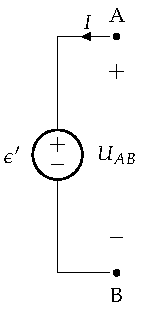
\includegraphics[height=3.5cm]{../figs/receptor_ideal.pdf}}\hfil
			\subfloat[Real]{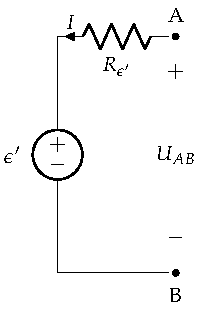
\includegraphics[height=3.5cm]{../figs/receptor_real.pdf}}
			\caption{Otros receptores}
			\label{fig.receptores}
		\end{figure}
	\end{itemize}
	
	\subsection{Eficiencia}
	Cualquier máquina, dispositivo, etc., tiene una \textbf{eficiencia}\footnote{No deben confundirse los términos de \textbf{eficiencia} y \textbf{rendimiento}. Mientras que eficiencia es la relación entre potencias, el rendimiento es la relación entre energías.} %(o eficiencia), 
	que expresa el cociente entre la potencia de salida y la potencia de entrada. Puesto que todos los dispositivos/máquinas tienen pérdidas, se cumple \textbf{siempre} que el rendimiento es menor del 100\% (o 1, si se expresa en tanto por uno). En general, para la teoría de circuitos, interesa conocer el rendimiento de:
	\begin{itemize}
		\item Generadores:
		\begin{equation}
			\boxed{\eta_g (\%) = \frac{P_{u}}{P_{g}}\cdot 100}
		\end{equation}
		\item Receptores (fundamentalmente, motores):
		\begin{equation}
			\boxed{\eta_m (\%) = \frac{P_{u}}{P_{a}}\cdot 100}
		\end{equation}
	\end{itemize}
	
	\begin{example}\label{ex.motor-bt1}
	    \textbf{Un generador de corriente continua, $fem=500$ V y $0.75\Omega$ de resistencia, alimenta mediante una línea de cobre de 18 m$\Omega$ mm$^2$/m y 16 mm$^2$ de sección a un motor de 1 CV y rendimiento 74.49\%, situado a 1 km de distancia. Se pide determinar:
	    \begin{itemize}
	        \item Intensidad de corriente en el motor y densidad de corriente, sabiendo que ésta última no debe superar 2 A/mm$^2$
	        \item Tensiones en bornes del generador y del motor, así como la caída de tensión en la línea
	        \item $fcem$ del motor y su resistencia
	    \end{itemize}}
	    
	    El circuito eléctrico se muestra en la Figura~\ref{fig.ejemplo_BT1_motor}.
	    \begin{figure}[H]
	        \centering
	        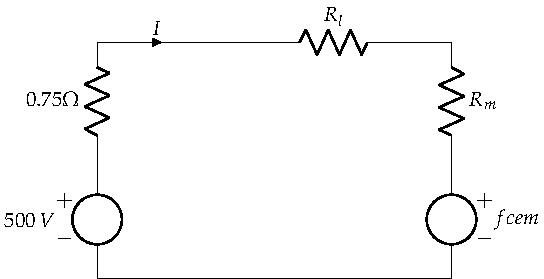
\includegraphics[width=0.5\linewidth]{../figs/ejemplo_BT1_motor.pdf}
	        \caption{Circuito eléctrico equivalente del Ejemplo~\ref{ex.motor-bt1}}
	        \label{fig.ejemplo_BT1_motor}
	    \end{figure}
	    La potencia útil del motor es 1 CV $=736$ W. La potencia absorbida, a partir del rendimiento: 
	    \begin{equation*}
	        P_{abs,M}=\dfrac{P_{u,M}}{\eta_M}=\dfrac{736}{0.7449}=988.05\;\text{W}=U_M\,I\Rightarrow U_M =\dfrac{988.05}{I}
	    \end{equation*}
	    siendo $U_M$ la tensión en el motor (motor + resistencia del motor). La resistencia de la línea es:
	    \begin{equation*}
	        R_l=2\,\rho\dfrac{l}{S}=2\cdot 18\cdot 10^{-3}\dfrac{1000}{16}= 2.25\Omega
	    \end{equation*}
	    Aplicando la 2LK al circuito completo, se obtiene que: 
	    \begin{equation*}
	        \epsilon_g-R_g\,I-R_l\,I-U_M=500-0.75\cdot I -2.25\cdot I-\dfrac{988.05}{I}=0\Rightarrow \begin{cases}
	            I_1=164.67\,\text{A}\\
	            I_2=2\,\text{A}
	        \end{cases}
	    \end{equation*}
	    
	    Con estos valores de corriente, se calcula la densidad para que cumpla la condición de densidad estipulada: 
	    \begin{align*}
	        \delta_1&=\dfrac{I_1}{S}=\dfrac{164.67}{16}=10.29\,\text{A/mm}^2>2\,\text{A/mm}^2\\
	        \delta_2&=\dfrac{I_2}{S}=\dfrac{2}{16}={0.13\,\text{A/mm}^2 < 2\,\text{A/mm}^2}
	    \end{align*}
	    Por tanto:
	    \begin{align*}
	        I&=2\,\text{A}\\
	        \delta&=0.13\,\text{A/mm}^2
	    \end{align*}
	    
	    Una vez conocida la corriente, la tensión en bornes del generador y motor son:
	    \begin{align*}
	        U_M&=\dfrac{P_{abs,M}}{I}=\dfrac{988.05}{2}=494.03\,\text{V}\\
	        U_l&=R_l\cdot I=2.25\cdot 2=4.5\,\text{V}\\
	        U_g&=U_M+U_l=494.03+4.5=498.53\,\text{V}
	    \end{align*}
	    
	    Por definición, la potencia útil del motor es:
	    \begin{equation*}
	        P_{u,M}=fcem\, I\Rightarrow {fcem=\dfrac{P_{u,M}}{I}=\dfrac{736}{2}=368\,\text{V}}
	    \end{equation*}
	    y la resistencia del mismo, a partir de la tensión $U_M$:
	    \begin{equation*}
	        U_M=fcem+R_M\,I\Rightarrow {R_M=\dfrac{U_M-fcem}{I}=\dfrac{494.03-368}{2}=63.02\;\Omega}
	    \end{equation*}
	    
	\end{example}
	
	\section{Asociación de elementos}
	
	Los diferentes elementos (tanto los activos como los pasivos) se pueden asociar de diferentes formas según la conexión que se haga entre ellos. 
	
	\subsection{Conexión en serie}
	Se dice que dos o más elementos están acoplados en \textbf{serie} cuando el final del primero se conecta al principio del segundo, el final del segundo al principio del tercero, y así sucesivamente. Es decir, varios elementos están conectados en serie cuando por ellos circula la \textbf{misma corriente}. 
	
	\subsubsection{Resistencias}
	Siguiendo el circuito de la Figura~\ref{fig.serie}, se cumple que:
		\begin{align*}
			u_1(t) &= R_1 \cdot i(t)\\
			u_2(t) &= R_2 \cdot i(t)\\
			u_3(t) &= R_3 \cdot i(t)
		\end{align*}
		\begin{figure}[H]
			\centering
			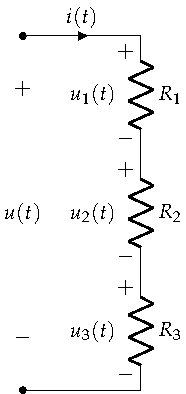
\includegraphics[width=0.2\linewidth]{../figs/AsociacionSerie.pdf}
			\caption{Conexión de resistencias en serie}
			\label{fig.serie}
		\end{figure}
		Al aplicar la 2LK, se obtiene que: 
		\begin{equation*}
			u(t) = u_1(t) + u_2(t) + u_3(t)
		\end{equation*}
		y sacando $i(t)$ como factor común, queda:
		\begin{equation*}
			u(t) = i(t) \cdot (R_1 + R_2 + R_3)
		\end{equation*}
		Por tanto, se puede definir la resistencia equivalente $R_{eq}$ de la conexión en serie como:
		\begin{equation}
			\boxed{R_{eq} = \sum_{i = 1}^n R_i}
		\end{equation}
		de modo que:
		\begin{equation*}
			u(t) = R_{eq} \cdot i(t)
		\end{equation*}
		
		Además, de las ecuaciones anteriores se tiene:
		\begin{align*}
			i(t) = \dfrac{u(t)}{R_1 + R_2 + R_3}
		\end{align*}
		pudiendo calcular la tensión de cualquiera de las resistencias como: 
		\begin{equation*}
			u_i(t) = R_i \cdot i(t)
		\end{equation*}
		Por tanto, la tensión parcial $u_i(t)$ se puede expresar en función de la tensión total $u(t)$ como: 
		\begin{equation*}
			u_i(t) = u(t) \cdot \frac{R_i}{R_1 + R_2 + R_3}
		\end{equation*}
		conocido como \textbf{divisor de tensión}. En general, para un circuito en serie:
		\begin{equation}
			\boxed{u_i(t) = u(t) \cdot \frac{R_i}{R_{eq}}}
		\end{equation}
		\subsubsection{Bobinas}
		Siguiendo el circuito de la Figura~\ref{fig.bobinas-serie}, se cumple que:
		\begin{align*}
			u_1(t) &= L_1 \cdot \dfrac{di(t)}{dt}\\
			u_2(t) &= L_2 \cdot \dfrac{di(t)}{dt}\\
			u_3(t) &= L_3 \cdot \dfrac{di(t)}{dt}\\
		\end{align*}
		\begin{figure}[H]
			\centering
			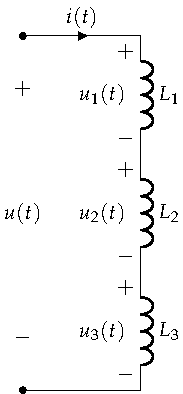
\includegraphics[width=0.2\linewidth]{../figs/BobinasSerie.pdf}
			\caption{Conexión de bobinas en serie}
			\label{fig.bobinas-serie}
		\end{figure}
		De manera análoga a las resistencias, al aplicar la 2LK se obtiene que: 
		\begin{equation*}
			u(t) = u_1(t) + u_2(t) + u_3(t)
		\end{equation*}
		y sacando $\frac{di(t)}{dt}$ como factor común, queda:
		\begin{equation*}
			u(t) = \dfrac{di(t)}{dt} \cdot (L_1 + L_2 + L_3)
		\end{equation*}
		por lo que se puede definir la inductancia equivalente $L_{eq}$ de la conexión en serie como:
		\begin{equation}
			\boxed{L_{eq} = \sum_{i = 1}^n L_i}
		\end{equation}
		de modo que:
		\begin{equation*}
			u(t) = L_{eq} \cdot \dfrac{di(t)}{dt}
		\end{equation*}
		\subsubsection{Condensadores}
		Con el circuito de la Figura~\ref{fig.condensadores-serie}, se cumple que:
		\begin{align*}
			i(t) &= C_1 \cdot \frac{du_1(t)}{dt}\\
			i(t) &= C_2 \cdot \frac{du_2(t)}{dt}\\
			i(t) &= C_3 \cdot \frac{du_3(t)}{dt}\\
		\end{align*}
		\begin{figure}[H]
			\centering
			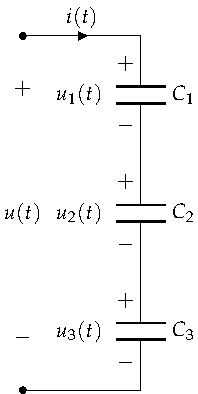
\includegraphics[width=0.2\linewidth]{../figs/CondensadoresSerie.pdf}
			\caption{Conexión de condensadores en serie}
			\label{fig.condensadores-serie}
		\end{figure}
		Al aplicar la 2LK se obtiene que: 
		\begin{equation*}
			u(t) = u_1(t) + u_2(t) + u_3(t)
		\end{equation*}
		Suponiendo que la carga sea nula en el instante inicial (para que las constantes de integración sean nulas) y sacando factor común $\int i(t)\,dt$, se tiene:
		\begin{equation*}
			u(t)=\left(\dfrac{1}{C_1}+\dfrac{1}{C_2}+\dfrac{1}{C_3} \right)\cdot \int i(t) dt
		\end{equation*}
		por lo que se puede definir la capacidad equivalente $C_{eq}$ de la conexión en serie como:
		\begin{equation}
			\boxed{\dfrac{1}{C_{eq}} = \sum_{i = 1}^n \dfrac{1}{C_i}}
		\end{equation}
		de modo que:
		\begin{equation*}
			i(t) = C_{eq} \cdot \frac{du(t)}{dt}
		\end{equation*}
		
		\subsubsection{Fuentes de tensión}
		
		Pueden conectarse en serie sin que exista \textbf{ninguna restricción}, independientemente de que se considere su modelo ideal o real. Su f.e.m. equivalente será la suma de cada una de las f.e.m.s. (por la 2LK) y, la resistencia equivalente, la suma de las resistencias internas de cada generador (en caso de considerar el modelo real).
		
		\subsubsection{Fuentes de corriente} 
		
		Hay que hacer diferencia entre si se considera el modelo ideal o el real:
		\begin{itemize}
			\item \textbf{Ideal.} Las fuentes de corriente ideales pueden conectarse en serie si, y sólo si, todas las fuentes suministran \textbf{igual intensidad y en el mismo sentido} (por la 1LK).
			\item \textbf{Real.} No existe ninguna restricción, llegando al generador equivalente mediante trasformación de fuentes (ver Sección~\ref{sec.dualidad}). 
		\end{itemize}
	
	\subsection{Conexión en paralelo}
	Se dice que dos o más elementos están acoplados en \textbf{paralelo} cuando todos los principios están conectados a un mismo punto, y todos los finales lo están en otro. Es decir, varios elementos están conectados en paralelo cuando todos ellos se encuentran sometidos a la \textbf{misma diferencia de potencial}.
	
			\subsubsection{Resistencias} 
			
			Con el circuito de la Figura~\ref{fig.resistencias-paralelo}, se cumple que:
		\begin{align*}
			i_1(t) &= \dfrac{u(t)}{R_1}\\
			i_2(t) &= \dfrac{u(t)}{R_2}\\
			i_3(t) &= \dfrac{u(t)}{R_3}\\
		\end{align*}
		\begin{figure}[H]
			\centering
			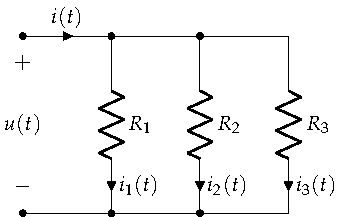
\includegraphics[width=0.35\linewidth]{../figs/AsociacionParalelo.pdf}
			\caption{Conexión de resistencias en paralelo}
			\label{fig.resistencias-paralelo}
		\end{figure}
		Al aplicar la 1LK, se obtiene que: 
		\begin{equation*}
			i(t) = i_1(t) + i_2(t) + i_3(t)
		\end{equation*}
		y sacando $u(t)$ como factor común, queda:
		\begin{equation*}
			i(t) = u(t) \cdot \left(\frac{1}{R_1} + \frac{1}{R_2} + \frac{1}{R_3}\right)
		\end{equation*}
		Por tanto, se puede definir la resistencia equivalente $R_{eq}$ de la conexión en paralelo como:
		\begin{equation}
			\boxed{\dfrac{1}{R_{eq}} = \sum_{i = 1}^n \dfrac{1}{R_i}}
		\end{equation}
		de modo que:
		\begin{equation*}
			u(t) = R_{eq} \cdot i(t)
		\end{equation*}
		
		\begin{remark}
			En el caso concreto de \textbf{dos resistencias} en paralelo, la expresión sería: 
			\begin{equation*}
				R_{eq}=\dfrac{1}{\frac{1}{R_1}+\frac{1}{R_2}}=\dfrac{1}{\frac{R_2+R_1}{R_1\cdot R_2}}=\dfrac{R_1\cdot R_2}{R_1+R_2}
			\end{equation*}
		\end{remark}
		
		Se define la \textbf{conductancia} $G$ [S] como la inversa de la resistencia. Así, en lugar de:
		\begin{equation*}
			\dfrac{1}{R_{eq}} = \sum_{i = 1}^n \dfrac{1}{R_i}
		\end{equation*}
		\begin{equation*}
			u(t) = R_{eq} \cdot i(t)
		\end{equation*}
		se puede escribir:
		\begin{equation}
			\boxed{G_{eq} = \sum_{i = 1}^n G_i}
		\end{equation}
		\begin{equation*}
			i(t) = G_{eq} \cdot u(t)
		\end{equation*}
		
		Además, de las ecuaciones anteriores (usando la conductancia) se tiene:
		\begin{align*}
			u(t) = \dfrac{i(t)}{G_1 + G_2 + G_3}
		\end{align*}
		pudiendo calcular la corriente de cualquiera de las resistencias como: 
		\begin{equation*}
			i_i(t) = G_i \cdot u(t)
		\end{equation*}
		Por tanto, la corriente parcial $i_i(t)$ se puede expresar en función de la corriente total $i(t)$ como: 
		\begin{equation*}
			i_i(t) = i(t) \cdot \dfrac{G_i}{G_1 + G_2 + G_3}
		\end{equation*}
		conocido como \textbf{divisor de corriente}. En general, para un circuito en paralelo:
		\begin{equation}
			\boxed{i_i(t) = i(t) \cdot \frac{G_i}{G_{eq}}}
		\end{equation}
		
		\subsubsection{Bobinas}
		
		Considerando el circuito de la Figura~\ref{fig.bobinas-paralelo}, se cumple que:
		\begin{align*}
			u(t) &= L_1 \cdot \frac{di_1(t)}{dt}\\
			u(t) &= L_2 \cdot \frac{di_2(t)}{dt}\\
			u(t) &= L_3 \cdot \frac{di_3(t)}{dt}\\
		\end{align*}
		\begin{figure}[H]
			\centering
			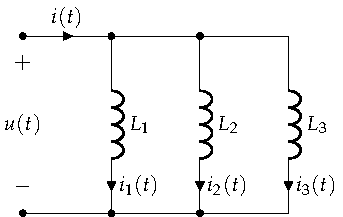
\includegraphics[width=0.35\linewidth]{../figs/BobinasParalelo.pdf}
			\caption{Conexión de bobinas en paralelo}
			\label{fig.bobinas-paralelo}
		\end{figure}
		Al aplicar la 1LK, se obtiene que: 
		\begin{equation*}
			i(t) = i_1(t) + i_2(t) + i_3(t)
		\end{equation*}
		y, suponiendo que la carga sea nula en el instante inicial (para que las constantes de integración sean nulas) y sacando factor común $\int u(t)\,dt$, se tiene:
		\begin{equation*}
			i(t)=\left(\dfrac{1}{L_1}+\dfrac{1}{L_2}+\dfrac{1}{L_3} \right)\cdot \int u(t) dt
		\end{equation*}
		Por tanto, se puede definir la inductancia equivalente $L_{eq}$ de la conexión en paralelo como:
		\begin{equation}
			\boxed{\dfrac{1}{L_{eq}} = \sum_{i = 1}^n \dfrac{1}{L_i}}
		\end{equation}
		de manera que:
		\begin{equation*}
			u(t) = L_{eq} \cdot \dfrac{di(t)}{dt}
		\end{equation*}
		\subsubsection{Condensadores} 
		Con el circuito de la Figura~\ref{fig.condensadores-paralelo}, se cumple que:
		\begin{align*}
			i_1(t) &= C_1 \cdot \frac{du(t)}{dt}\\
			i_2(t) &= C_2 \cdot \frac{du(t)}{dt}\\
			i_3(t) &= C_3 \cdot \frac{du(t)}{dt}\\
		\end{align*}
		\begin{figure}[H]
			\centering
			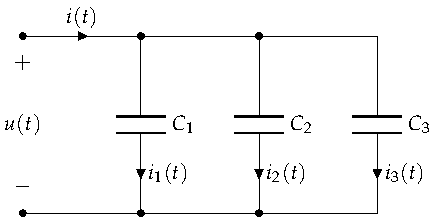
\includegraphics[width=0.4\linewidth]{../figs/CondensadoresParalelo.pdf}
			\caption{Conexión de condensadores en paralelo}
			\label{fig.condensadores-paralelo}
		\end{figure}
		Al aplicar la 1LK se obtiene que: 
		\begin{equation*}
			i(t) = i_1(t) + i_2(t) + i_3(t)
		\end{equation*}
		por lo que, sacando factor común $\frac{du(t)}{dt}$, se tiene:
		\begin{equation*}
			i(t)=C_1\cdot \dfrac{du(t)}{dt}+ C_2\cdot \dfrac{du(t)}{dt}+ C_3\cdot \dfrac{du(t)}{dt}=(C_1+C_2+C_3)\cdot\dfrac{du(t)}{dt}
		\end{equation*}
		por lo que se puede definir la capacidad equivalente $C_{eq}$ de la conexión en paralelo como:
		\begin{equation}
			\boxed{C_{eq} = \sum_{i = 1}^n C_i}
		\end{equation}
		de modo que:
		\begin{equation*}
			i(t) = C_{eq} \cdot \frac{du(t)}{dt}
		\end{equation*}
		
		\subsubsection{Fuentes de tensión}
		
		Hay que hacer diferencia entre si se considera el modelo ideal o el real:
		\begin{itemize}
			\item \textbf{Ideal.} Las fuentes de tensión ideales pueden conectarse en paralelo si, y sólo si, todas las fuentes tienen \textbf{igual f.e.m. y ésta actúa en el mismo sentido}.
			\item \textbf{Real.} No existe \textbf{ninguna restricción}, llegando al generador equivalente mediante trasformación de fuentes (ver Sección~\ref{sec.dualidad}). 
		\end{itemize}
		
		\subsubsection{Fuentes de corriente}
		
		Pueden conectarse en paralelo sin que exista ninguna restricción, independientemente de que se considere su modelo ideal o real. Su intensidad equivalente será la suma de cada una de las intensidades, y la resistencia equivalente se calculará a partir del paralelo entre varias resistencias (en caso de considerar el modelo real).
	
	
	\begin{example}\label{ex.serie-paralelo}
	    \textbf{Calcular la corriente que pasa por la fuente de tensión de la Figura \ref{fig.ejercicio1_tema1}.}
		\begin{figure}[H]
			\centering
			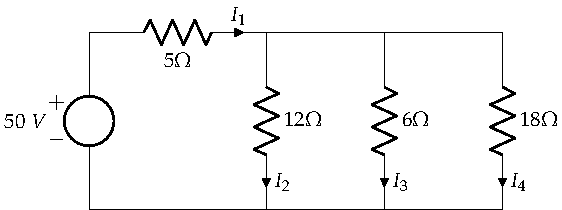
\includegraphics{../figs/ej1_BT1.pdf}
			\caption{Ejemplo~\ref{ex.serie-paralelo}}
			\label{fig.ejercicio1_tema1}
		\end{figure}
		
		Se pide calcular la corriente $I_1$. Se empiezan asociando las tres resistencias en paralelo de 12, 6 y 18~$\Omega$:
\begin{equation*}
    R_{eq,||}=\dfrac{1}{\frac{1}{R_{12}}+\frac{1}{R_{6}}+\frac{1}{R_{18}}}=\dfrac{1}{\frac{1}{12}+\frac{1}{6}+\frac{1}{18}}=3.273\,\Omega
\end{equation*}
La resistencia equivalente total:
\begin{equation*}
    R_{eq}=R_5+R_{eq,||}=5+3.273=8.273\,\Omega
\end{equation*}
Por la ley de Ohm: 
\begin{equation*}
    I_1=\dfrac{U}{R_{eq}}=\dfrac{50}{8.273}={6.04\,\text{A}}
\end{equation*}
	\end{example}
	
	
	
	\subsection{Conexión estrella-triángulo}
	Estas dos configuraciones tienen una importancia fundamental en la teoría de circuitos, ya que son las dos posibilidades de conexión de cargas trifásicas. En la Figura~\ref{fig.estrella-triangulo} se muestran estas redes pasivas, cuyos terminales de acceso exterior
	se han denominado $A$, $B$ y $C$ y que tienen la misma situación ``topográfica''. La conexión triángulo está
	formada por tres resistencias $R_{ab}$, $R_{bc}$ y $R_{ca}$, que unen los diversos nudos, dando la apariencia
	geométrica de un triángulo. Por su parte, la conexión
	estrella representa tres resistencias $R_a$, $R_b$ y $R_c$, que parten de los tres nudos de acceso
	externo $A$, $B$ y $C$, y que se unen en un punto común $N$. 
	\begin{figure}[H]
		\centering
		\subfloat[Conexión triángulo]{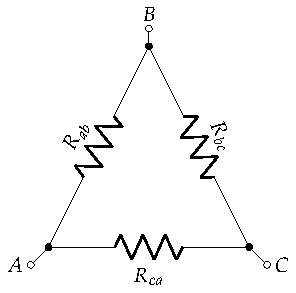
\includegraphics[width=0.3\linewidth]{../figs/Conexion_Triangulo.pdf}}\hfil
		\subfloat[Conexión estrella]{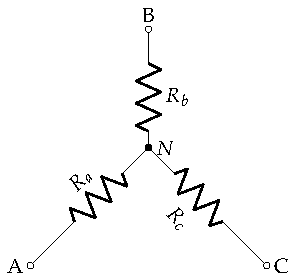
\includegraphics[width=0.3\linewidth]{../figs/Conexion_Estrella.pdf}}
		\caption{Conexión en estrella y en triángulo}
		\label{fig.estrella-triangulo}
	\end{figure}
	
	Lo interesante es buscar las leyes de transformación de una red a la otra, de tal modo que ambos circuitos sean equivalentes desde el punto de vista externo (es decir,
	desde los nudos $A$, $B$ y $C$). Está claro que, si las dos redes son equivalentes, deberán consumir las mismas
	corrientes cuando se aplican las mismas tensiones externas, lo que equivale a decir que las resistencias que se observan entre los diferentes terminales $A-B$, $B-C$ y $C-A$ deben ser idénticas para ambos montajes y, por consiguiente, se
	deben satisfacer las igualdades mostradas en la Tabla~\ref{tab.igualdades_estrellatriangulo}. 
	\begin{table}[H]
		\centering
		\begin{tabular}{c|c|c} \textbf{Resistencia} & \textbf{Estrella} & \textbf{Triángulo}\\\hline
			&&        \\[-0.75em]
			$R_{AB}$ & $R_a+R_b$ & $\dfrac{R_{ab} \cdot (R_{bc} + R_{ca})}{R_{ab} + R_{bc} + R_{ca}}$\\
			&&         \\[-0.75em]
			$R_{AB}$ & $R_b+R_c$ & $\dfrac{R_{bc} \cdot (R_{ab} + R_{ca})}{R_{ab} + R_{bc} + R_{ca}}$\\
			&& \\[-0.75em]
			$R_{CA}$ & $R_a+R_c$ & $\dfrac{R_{ca} \cdot (R_{ab} + R_{bc})}{R_{ab} + R_{bc} + R_{ca}}$\\
		\end{tabular}
		\caption{Igualdades que se deben satisfacer para la equivalencia estrella-triángulo}
		\label{tab.igualdades_estrellatriangulo}
	\end{table}
	
	A partir de la Tabla~\ref{tab.igualdades_estrellatriangulo}, se obtiene que las resistencias vistas desde los diferentes nudos, en la conexión triángulo, son:
	\begin{align*}
		R_{AB} &= \frac{R_{ab} \cdot R_{bc}}{R_{ab} + R_{bc} + R_{ca}} + \frac{R_{ab} \cdot R_{ca}}{R_{ab} + R_{bc} + R_{ca}}\\
		\\
		R_{BC} &= \frac{R_{bc} \cdot R_{ab}}{R_{ab} + R_{bc} + R_{ca}} + \frac{R_{bc} \cdot R_{ca}}{R_{ab} + R_{bc} + R_{ca}}\\
		\\
		R_{CA} &= \frac{R_{ca} \cdot R_{ab}}{R_{ab} + R_{bc} + R_{ca}} + \frac{R_{ca} \cdot R_{bc}}{R_{ab} + R_{bc} + R_{ca}}
	\end{align*}
	que deben ser igual a las de estrella:
	\begin{align*}
		\dfrac{R_{a{\color{magenta}b}} \cdot R_{{\color{magenta}b}c}}{R_{ab} + R_{bc} + R_{ca}} + \dfrac{R_{{\color{teal}a}b} \cdot R_{c{\color{teal}a}}}{R_{ab} + R_{bc} + R_{ca}} &= R_{\color{teal}a} + R_{\color{magenta}b}\\
		\\
		\dfrac{R_{a{\color{magenta}b}} \cdot R_{{\color{magenta}b}c}}{R_{ab} + R_{bc} + R_{ca}} + \dfrac{R_{b{\color{orange}c}} \cdot R_{{\color{orange}c}a}}{R_{ab} + R_{bc} + R_{ca}} &= R_{\color{magenta}b} + R_{\color{orange}c}\\
		\\
		\dfrac{R_{{\color{teal}a}b} \cdot R_{c{\color{teal}a}}}{R_{ab} + R_{bc} + R_{ca}} + \dfrac{R_{b{\color{orange}c}} \cdot R_{{\color{orange}c}a}}{R_{ab} + R_{bc} + R_{ca}} &= R_{\color{orange}c} + R_{\color{teal}a}
	\end{align*}
	Igualando y operando, se llega a las siguientes relaciones: 
	\begin{itemize}
		\item \textbf{Conversión de triángulo a estrella:} 
		\begin{align}
			\Aboxed{R_a &= \frac{R_{ab} \cdot R_{ca}}{R_{ab} + R_{bc} + R_{ca}}}\\[10pt]
			\Aboxed{R_b &= \frac{R_{ab} \cdot R_{bc}}{R_{ab} + R_{bc} + R_{ca}}}\\[10pt]
			\Aboxed{R_c &= \frac{R_{bc} \cdot R_{ca}}{R_{ab} + R_{bc} + R_{ca}}}
		\end{align}
		\item \textbf{Conversión de estrella a triángulo:}
		\begin{align}
			\Aboxed{G_{ab} &= \frac{G_a \cdot G_b}{G_a + G_b + G_c}}\\[10pt]
			\Aboxed{G_{bc} &= \frac{G_b \cdot G_c}{G_a + G_b + G_c}}\\[10pt]
			\Aboxed{G_{ca} &= \frac{G_c \cdot G_a}{G_a + G_b + G_c}}
		\end{align}
	\end{itemize}
	
	Las transformaciones anteriores se utilizan con gran frecuencia en el análisis de circuitos, ya que permiten simplificar ciertas redes en las que las resistencias no están
	conectadas de forma simple (en serie o en paralelo). Quiere destacarse que, en caso de que las resistencias sean iguales ($R_a=R_b=R_c=R_Y$ para la estrella y $R_{ab}=R_{bc}=R_{ca}=R_D$ para el triángulo), se cumple que: 
	\begin{equation}\label{eq.triangulo-estrella-igual}
		\boxed{R_D=3\cdot R_Y}
	\end{equation}
	
	%\newpage
	\begin{example}\label{ex.estrella-triangulo}
	\textbf{Convertir los circuitos de la Figura~\ref{fig.ejercicio7-bt1} en triángulo o estrella equivalente, según corresponda. }
 \begin{figure}[H]
 		\centering
\includegraphics[height=3.5cm]{../figs/ej7_BT1.pdf}
 		\caption{Ejemplo~\ref{ex.estrella-triangulo}}
 		\label{fig.ejercicio7-bt1}
 	\end{figure}
 	
 	Se calcula primero el cambio de estrella a triángulo. Puesto que las tres resistencias tienen un valor de 60 $\Omega$ ($R_a=R_b=R_c=R_Y=60\Omega$), se cumple que, según~\eqref{eq.triangulo-estrella-igual}: 
	\begin{equation*}
		R_D=3\cdot R_Y=3\cdot 60=180\Omega
	\end{equation*}
	Puede comprobarse que se llegaría a la misma solución empleando las expresiones completas, donde $G_i=\frac{1}{R_i}=\frac{1}{60}$ S: 
	\begin{align*}
			G_{ab} &= \frac{G_a \cdot G_b}{G_a + G_b + G_c}=\frac{\frac{1}{60} \cdot \frac{1}{60}}{\frac{1}{60} + \frac{1}{60} + \frac{1}{60}}=5.55\cdot 10^{-3}\,\text{S}\Rightarrow R_{ab}=\dfrac{1}{G_{ab}}=\dfrac{1}{5.55\cdot 10^{-3}}=180\Omega\\[10pt]
			G_{bc} &= \frac{G_b \cdot G_c}{G_a + G_b + G_c}=\frac{\frac{1}{60} \cdot \frac{1}{60}}{\frac{1}{60} + \frac{1}{60} + \frac{1}{60}}=5.55\cdot 10^{-3}\,\text{S}\Rightarrow R_{bc}=\dfrac{1}{G_{bc}}=\dfrac{1}{5.55\cdot 10^{-3}}=180\Omega\\[10pt]
			G_{ca} &= \frac{G_c \cdot G_a}{G_a + G_b + G_c}\frac{\frac{1}{60} \cdot \frac{1}{60}}{\frac{1}{60} + \frac{1}{60} + \frac{1}{60}}=5.55\cdot 10^{-3}\,\text{S}\Rightarrow R_{ca}=\dfrac{1}{G_{ca}}=\dfrac{1}{5.55\cdot 10^{-3}}=180\Omega
		\end{align*}

El cambio de triángulo a estrella debe hacerse a partir de las ecuaciones completas, puesto que sus resistencias son todas diferentes: 
\begin{align*}
			R_a &= \frac{R_{ab} \cdot R_{ca}}{R_{ab} + R_{bc} + R_{ca}}=\frac{10 \cdot 20}{10 + 30 + 20}=\frac{10}{3}\Omega\\
			\\
			R_b &= \frac{R_{ab} \cdot R_{bc}}{R_{ab} + R_{bc} + R_{ca}}=\frac{10 \cdot 30}{10+30+20}=5\Omega\\
			\\
			R_c &= \frac{R_{bc} \cdot R_{ca}}{R_{ab} + R_{bc} + R_{ca}}=\frac{30 \cdot 20}{10+30+20}=10\Omega
		\end{align*}

Los circuitos equivalentes son los mostrados en la Figura~\ref{fig.ejercicio7-bt1-sol}.
 \begin{figure}[H]
 		\centering
\includegraphics[height=3.5cm]{../figs/ej7_BT1_sol.pdf}% 
 		\caption{Ejemplo~\ref{ex.estrella-triangulo} -- Solución}
 		\label{fig.ejercicio7-bt1-sol}
 	\end{figure}
	    
	\end{example}
	
	\section{Aplicación de las leyes de Kirchhoff: métodos de análisis} \label{sec.metodos_analisis_cc}
	Para resolver un circuito, se debe conocer $U$ e $I$ en cada una de sus ramas. Por tanto, si se tiene un circuito formado por $r$ ramas, el número de incógnitas será $2\cdot r$ (una de tensión y otra de intensidad). Por tanto, para resolver el circuito se deben disponer de $2\cdot r$ ecuaciones linealmente independientes. Para ello, basta con aplicar las leyes de Kirchhoff a los nudos y mallas del circuito. 
	
	\begin{example}
		\label{ej.1-4}
		\textbf{Plantear el sistema de ecuaciones para resolver el circuito de la Figura~\ref{fig.mallas1}.}
		\begin{figure}[H]
			\centering
			\includegraphics[width=0.5\linewidth]{../figs/mallas1.pdf}
			\caption{Ejemplo~\ref{ej.1-4}}
			\label{fig.mallas1}
		\end{figure}
		
		\begin{enumerate}
			\item {Se aplica la 1LK:} 
			\begin{itemize}
				\item {Nudo A:} $I_6 = I_1 + I_2$
				\item {Nudo B:} $I_1 + I_3 + I_5 = 0$
				\item {Nudo C:} $I_2 = I_3 + I_4$
				\item {Nudo D:} $I_4 = I_5 + I_6$
			\end{itemize}
			Sin embargo, se observa que no son ecuaciones linealmente independientes, puesto que $C=A+B+D$.
			\item {Se aplica la 2LK:}
			\begin{itemize}
				\item {Malla ABCA:} $I_1 \cdot R_1 - \epsilon_1 + \epsilon_2 - I_3 \cdot R_3 - I_2 \cdot R_2 = 0$
				\item {Malla BDCB:} $-I_5 \cdot R_5 - I_4 \cdot R_4 + I_3 \cdot R_3 - \epsilon_2 = 0$
				\item {Malla ACDA:} $I_2 \cdot R_2 + I_4 \cdot R_4 + I_6 \cdot R_6 - \epsilon_3 = 0$
			\end{itemize}
			\item {Se combinan las ecuaciones:}
			\begin{align*}
				- I_1 -  I_2 + I_6  &= 0\\
				I_1 + I_3 + I_5 &= 0\\
				I_4 - I_5 - I_6 &= 0\\
				I_1 \cdot R_1 - I_2 \cdot R_2 - I_3 \cdot R_3 &= \epsilon_1 - \epsilon_2\\
				I_3 \cdot R_3 - I_4 \cdot R_4 -I_5 \cdot R_5 &= \epsilon_2\\
				I_2 \cdot R_2 + I_4 \cdot R_4 + I_6 \cdot R_6 &= \epsilon_3
			\end{align*}
			\item {Se expresan en forma matricial:}
			\begin{equation*}
				\begin{bmatrix}
					-1 & -1 & 0 & 0 & 0 & 1\\
					1 & 0 & 1 & 0 & 1 & 0\\
					0 & 0 & 0 & 1 & -1 & -1\\
					R_1 & -R_2 & - R_3 & 0 & 0 & 0\\
					0 & 0 & R_3 & - R_4 & - R_5 & 0\\
					0 & R_2 & 0 & R_4 & 0 & R_6
				\end{bmatrix} \cdot %
				\begin{bmatrix}
					I_1\\
					I_2\\
					I_3\\
					I_4\\
					I_5\\
					I_6    
				\end{bmatrix} = %
				\begin{bmatrix}
					0\\
					0\\
					0\\
					\epsilon_1 - \epsilon_2\\
					\epsilon_2\\
					\epsilon_3
				\end{bmatrix}
			\end{equation*}
		\end{enumerate}
		Se observa que es necesario resolver un sistema lineal de 6 ecuaciones en las que las incógnitas son las corrientes de cada rama. 
	\end{example}
	
	Esta forma de resolución de circuitos eléctricos, aunque es válida, no es útil por el número de ecuaciones a resolver. Por ello, lo más habitual es utilizar otros métodos que permiten la resolución de los circuitos con un número menor de ecuaciones. Aunque existen diferentes métodos, se van a presentar dos: el método de las mallas y el método de los nudos, explicando posteriormente una modificación de este último.
	
	\subsection{Método de las mallas}
	El método de las mallas simplifica el sistema de ecuaciones necesario mediante unas corrientes \emph{ficticias} denominadas \textbf{corrientes de malla}, aprovechando las relaciones entre tensiones de la 2LK. El procedimiento general de aplicación de este método es el siguiente:
	\begin{enumerate}
		\item Identificar las corrientes de rama.
		\item Asignar un sentido a las corrientes de malla, teniendo en cuenta que hay un total de:
		\begin{equation*}
			{Mallas=Ramas-Nudos+1}
		\end{equation*}
		\item Relacionar corrientes de rama con corrientes de malla.
		\item Escribir ecuaciones de mallas.
		\item Resolver la ecuación, obteniendo las corrientes de malla.
		\item Obtener las corrientes de rama con las relaciones del punto 3.
	\end{enumerate}
	
	\begin{example}
		\label{ej.1-5}
		\textbf{Plantear el sistema de ecuaciones para resolver el circuito de la Figura~\ref{fig.mallas1}.}
		
		Se sigue el procedimiento indicado anteriormente, donde el punto 1 ya está indicado en el circuito de la Figura~\ref{fig.mallas1}: 
		\begin{enumerate}
			\item[2.] Asignar un sentido a las corrientes de malla: se muestra en la Figura~\ref{fig.mallas1_corrientes}
			\begin{figure}[H]
				\centering
				\includegraphics[width=0.5\linewidth]{../figs/mallas1_corrientes.pdf}
				\caption{Corrientes de malla del circuito del Ejemplo~\ref{ej.1-5}}
				\label{fig.mallas1_corrientes}
			\end{figure}
			\item[3.] Relacionar corrientes de rama con corrientes de malla:
			\begin{align*}
				I_1 &= I_a\\
				I_5 &= -I_b\\
				I_6 &= I_c\\
				I_2 &= I_c -I_a\\
				I_3 &= I_b - I_a\\
				I_4 &= I_c - I_b
			\end{align*}
			\item[4.] Escribir ecuaciones de mallas: 
			
			Malla ABCA: $I_a \cdot R_1 - \epsilon_1 + \epsilon_2 + (I_a - I_b) \cdot R_3 + (I_a - I_c) \cdot R_2 = 0$
			
			Malla BDCB: $I_b \cdot R_5 + (I_b - I_c) \cdot R_4 + (I_b - I_a) \cdot R_3 - \epsilon_2 = 0$
			
			Malla ACDA: $(I_c - I_a) \cdot R_2 + (I_c - I_b) \cdot R_4 + I_c \cdot R_6 - \epsilon_3 = 0$
			
			Se reagrupan las corrientes en las ecuaciones anteriores, obteniéndose que: 
			\begin{align*}
				I_a \cdot (R_1 + R_3 + R_2)  - I_b\cdot R_3 - I_c \cdot R_2 &= \epsilon_1 - \epsilon_2\\
				- I_a \cdot R_3 + I_b \cdot (R_5 + R_4 + R_3) - I_c \cdot R_4 &=  \epsilon_2\\
				- I_a \cdot R_2 - I_b \cdot R_4 + I_c \cdot (R_2 + R_4 + R_6) &= \epsilon_3
			\end{align*}
			que, en forma matricial: 
			\begin{equation*}
				\begin{bmatrix}
					(R_1 + R_3 + R_2) &  - R_3 & - R_2 \\
					- R_3 & (R_5 + R_4 + R_3) & - R_4 \\
					- R_2 & - R_4 &  (R_2 + R_4 + R_6)
				\end{bmatrix} \cdot %
				\begin{bmatrix}
					I_a\\
					I_b\\
					I_c\\
				\end{bmatrix} = %
				\begin{bmatrix}
					\epsilon_1 - \epsilon_2\\
					\epsilon_2\\
					\epsilon_3
				\end{bmatrix}
			\end{equation*}
		\end{enumerate}
	\end{example}
	
	A partir de este ejemplo, se llega a la ecuación general que permite determinar el sistema de ecuaciones de un circuito de $n$ mallas, siendo esta: 
	\begin{equation*}
		\begin{bmatrix}
			{\color{magenta}\sum R_{11}} &  {\color{teal}\pm\sum R_{12}} & {\color{teal}{\dots}} & {\color{teal}\pm\sum R_{1n}} \\
			{\color{teal}\pm\sum R_{21}} & {\color{magenta}\sum R_{22}} & {{\dots}} & {\color{teal}\pm\sum R_{2n}} \\
			{\vdots} & {\vdots} &  {\ddots} & \vdots\\
			{\color{teal}\pm\sum R_{n1}} & {\color{teal}\pm\sum R_{n2}} & \dots & {\color{magenta}\sum R_{nn}}
		\end{bmatrix} \cdot 
		\begin{bmatrix}
			I_1\\
			I_2\\
			\vdots\\
			I_n
		\end{bmatrix} = %
		\begin{bmatrix}
			{\color{orange}\sum\epsilon_1}\\
			{\color{orange}\sum\epsilon_2}\\
			{\color{orange}\vdots}\\
			{\color{orange}\sum\epsilon_n}
		\end{bmatrix}
	\end{equation*}
	donde cada {\color{magenta}$R_{ii}$} se corresponde con la suma de resistencias incluidas en la malla $i$; cada {\color{teal}$\pm R_{ij}$} se corresponde con la suma de las resistencias incluidas en las ramas compartidas por las mallas $i$ y $j$, con signo positivo ($+$) si las corrientes van en el mismo sentido, y negativo ($-$) en caso contrario; y cada {\color{orange} $\sum \epsilon_i$} es la suma algebraica de las fuerzas electromotrices de los generadores de la malla $i$, considerando un signo positivo ($+$) si contribuyen al giro de la corriente, y negativo ($-$) en caso contrario (es decir, si la corriente sale por el polo $+$ de la fuente, se considera positivo; si sale por el polo $-$, se considera negativo). Debe tenerse en cuenta que, para aplicar este método, \textbf{todos los generadores deben ser fuentes de tensión}. 
	
	\begin{example}\label{ex.ejemplo_mallas}
          \textbf{Resolver el circuito del ejemplo \ref{ej.1-5} con
            los siguientes valores numéricos.}

          \begin{minipage}{0.35\linewidth}
            Datos:
            \begin{align*}
              R_1 = R_3 = R_6 &= \SI{3}{\ohm}\\
              R_2 = R_4 = R_5 &= \SI{2}{\ohm}\\
              \epsilon_1 &= \SI{245}{\volt}\\
              \epsilon_2 &= \SI{490}{\volt}\\
              \epsilon_3 &= \SI{735}{\volt}\\
            \end{align*}
          \end{minipage}
          \begin{minipage}{0.55\linewidth}
            \includegraphics{../figs/mallas1_corrientes.pdf}
          \end{minipage}

          Sustituyendo los valores numéricos en las ecuaciones
          obtenidas en el ejemplo anterior obtenemos:
          \[
            \left[\begin{array}{ccc}
                    8 & -3 & -2 \\
                    -3 & 7 & -2 \\
                    -2 & -2 & 7\\
                  \end{array}\right]%
                \cdot \left[\begin{array}{c}
                              I_a\\
                              I_b\\
                              I_c\\
                            \end{array}\right]%
                          = \left[\begin{array}{c}
                                    -245\\
                                    490\\
                                    735
                                  \end{array}\right]
                              \]
                              cuya solución es:

\begin{align*}
  I_a &= \SI{65}{\ampere}\\
  I_b &= \SI{145}{\ampere}\\
  I_c &= \SI{165}{\ampere}
\end{align*}

Por tanto, los valores de las corrientes de rama son:

\begin{align*}
  I_1 &= \SI{65}{\ampere}\\
  I_2 &= \SI{100}{\ampere}\\
  I_3 &= \SI{80}{\ampere}\\
  I_4 &= \SI{20}{\ampere}\\
  I_5 &= \SI{-145}{\ampere}\\
  I_6 &= \SI{165}{\ampere}
\end{align*}
\end{example}
	
	\begin{remark}
	    El Ejemplo~\ref{ex.mallas_dependiente} incluye contenido avanzado que queda fuera del alcance de la asignatura.
	\end{remark}
	
	\begin{example}\label{ex.mallas_dependiente}
	    \textbf{Calcular la corriente $I$ en el circuito de la Figura~\ref{fig.ejemplo_mallas_dependiente}.}
	    \begin{figure}[H]
	        \centering
	        \includegraphics[width=0.35\linewidth]{../figs/ejemplo_mallas_dependiente.pdf}
	        \caption{Ejemplo~\ref{ex.mallas_dependiente}}
	        \label{fig.ejemplo_mallas_dependiente}
	    \end{figure}
	    
	    En este caso, no se puede transformar el generador de intensidad en uno de tensión, por lo que  se le asigna una caída de tensión arbitraria (y desconocida), $U_{g1}$, considerándolo como un generador de tensión. Posteriormente, al plantear el sistema de ecuaciones, se añadirá una ecuación adicional, puesto que la intensidad de esa rama es conocida (2 A). El circuito queda como se muestra en la Figura~\ref{fig.mallas_dpendiente_sol}.
	    \begin{figure}[H]
	        \centering
	        \includegraphics[width=0.35\linewidth]{../figs/ejemplo_mallas_dependiente_sol.pdf}
	        \caption{Ejemplo~\ref{ex.mallas_dependiente} -- Mallas}
	        \label{fig.mallas_dpendiente_sol}
	    \end{figure}
	    
	    Se plantea el método de mallas en forma matricial: 
	    \begin{equation*}
		\begin{bmatrix}
			5 & -2 \\
			-2 & 7 
		\end{bmatrix} \cdot 
		\begin{bmatrix}
			I_a\\
			I_b
		\end{bmatrix} = %
		\begin{bmatrix}
			-4-U_{g1} \\
			4-3\cdot U_r
		\end{bmatrix}
	\end{equation*}
	donde se sabe que $I_a=-2$ A. Además, la tensión $U_r$ se puede expresar, a partir d ela ley de Ohm y las relaciones entre las corrientes de malla como:
	\begin{equation*}
	    U_r=(I_a-I_b)\cdot R_{2\Omega}=(I_a-I_b)\cdot 2 = (-2-I_b)\cdot 2=-4-2\, I_b
	\end{equation*}
	Reemplazando en la segunda ecuación del sistema:
	\begin{equation*}
	    -2\, I_a+7\,I_b=4-3\,U_r; -2\,(-2)+7\, I_b=4-3\,(-4-2\,I_b); 4+7\,I_b=4+12+6\,I_b\Rightarrow I_b=12\, A 
	\end{equation*}
	    Por lo que $I=-I_b=-12$ A
	\end{example}
	

	
	\subsection{Método de los nudos}
	El método de los nudos es otro de los procedimientos de
        análisis utilizados en teoría de circuitos, aprovechando las
        relaciones entre corrientes de la 1LK. El procedimiento
        general de aplicación de este método es el siguiente:
	\begin{enumerate}
        \item Identificar las corrientes de rama.
        \item Identificar los nudos independientes, que son:
          \begin{equation*}
            {Nudos\;\;Independientes=Nudos-1}
          \end{equation*}
        \item Aplicar la 1LK a cada nudo independiente.
        \item Determinar las tensiones en los receptores a partir de
          la Ley de Ohm (considerando la resistencia y, después, la
          conductancia).
        \item Combinar las ecuaciones de los puntos 3 y 4.
        \item Resolver la ecuación.
	\end{enumerate}
	
	\begin{example}\label{ej.1-6}
          \textbf{Plantear el sistema de ecuaciones para resolver el
            circuito de la Figura~\ref{fig.nudos}.}
          \begin{figure}[H]
            \centering \includegraphics{../figs/nudos.pdf}
            \caption{Ejemplo~\ref{ej.1-6}}
            \label{fig.nudos}
          \end{figure}
		
          Se sigue el procedimiento indicado anteriormente, llegando
          únicamente hasta el punto 5:
		
          \begin{enumerate}
          \item Identificar las corrientes de rama: identificadas en
            la Figura~\ref{fig.nudos}
          \item Identificar los nudos independientes, que son $A$ y
            $B$ en la Figura~\ref{fig.nudos}.
          \item Aplicar la 1LK a cada nudo independiente:
			
            Nudo A
            \begin{equation*}
              I_{g1} - I_a - I_{ab} = 0
            \end{equation*}
			
            Nudo B
            \begin{equation*}
              I_{ab} - I_{g2} - I_b = 0
            \end{equation*}
          \item Determinar las tensiones en los receptores a partir de
            la Ley de Ohm (considerando la resistencia y, después, la
            conductancia):
            \begin{align*}
              U_A = U_{R_1} &= I_a \cdot R_1\rightarrow I_a=U_A\cdot G_1\\
              U_B = U_{R_3} &= I_b \cdot R_3\rightarrow I_b=U_B\cdot G_3\\
              U_{AB}=U_{R_2} &= I_{ab} \cdot R_2\rightarrow I_{ab}=(U_A-U_B)\cdot G_2\\
            \end{align*}
          \item Combinar las ecuaciones de los puntos 3 y 4:
			
            Nudo A
            \begin{equation*}
              I_{g1} - U_A \cdot G_1 - (U_A - U_B) \cdot G_2 = 0\rightarrow I_{g1} = U_A \cdot (G_1 + G_2) - U_B \cdot G_2 
            \end{equation*}
			
            Nudo B
            \begin{equation*}
              (U_A - U_B) \cdot G_2 - I_{g2} - U_B \cdot G_3 = 0 \rightarrow  - I_{g2} = - U_A \cdot G_2 + U_B \cdot (G_2 + G_3)
            \end{equation*}
			
            Estas ecuaciones se pueden expresar en forma matricial de
            la siguiente manera:
            \begin{equation*}
              \begin{bmatrix}
                G_1 + G_2 & - G_2\\
                -G_2 & G_2 + G_3
              \end{bmatrix} \cdot%
              \begin{bmatrix}
                U_A\\
                U_B
              \end{bmatrix} = %
              \begin{bmatrix}
                I_{g1}\\
                -I_{g2}
              \end{bmatrix}
            \end{equation*}
          \end{enumerate}
	\end{example}
	
	A partir de este ejemplo, se llega a la ecuación general que
        permite determinar el sistema de ecuaciones de un circuito de
        $n$ nudos, siendo esta:
	\begin{equation*}
          \begin{bmatrix}
            {\color{magenta}\sum G_{1}} &  {\color{teal}-\sum G_{12}} & {\color{teal}{\dots}} & {\color{teal}-\sum G_{1n}} \\
            {\color{teal}-\sum G_{21}} & {\color{magenta}\sum G_{2}} & {{\dots}} & {\color{teal}-\sum G_{2n}} \\
            {\vdots} & {\vdots} &  {\ddots} & \vdots\\
            {\color{teal}-\sum G_{n1}} & {\color{teal}-\sum G_{n2}} & \dots & {\color{magenta}\sum G_{n}}
          \end{bmatrix} \cdot 
          \begin{bmatrix}
            U_1\\
            U_2\\
            \vdots\\
            U_n
          \end{bmatrix} = %
          \begin{bmatrix}
            {\color{orange}\sum I_{g1}}\\
            {\color{orange}\sum I_{g2}}\\
            {\color{orange}\vdots}\\
            {\color{orange}\sum I_{gn}}
          \end{bmatrix}
	\end{equation*}
	donde cada {\color{magenta}$G_{i}$} se corresponde con la suma
        de conductancias conectadas al nudo $i$; cada
        {\color{teal}$ G_{ij}$} se corresponde con la suma de las
        conductancias conectadas entre los nudos $i$ y $j$; y cada
        {\color{orange} $\sum I_{gi}$} es la suma algebraica de las
        corrientes de los generadores conectados al nudo $i$,
        considerando un signo positivo ($+$) si el generador inyecta
        corriente en el nudo, y negativo ($-$) en caso contrario. Debe
        tenerse en cuenta que para aplicar este método \textbf{todos
          los generadores deben ser fuentes de corriente}.
	
	\begin{example}\label{ex.nudos}
          \textbf{En el circuito de la Figura~\ref{fig.nudos_fuentes}
            se debe emplear el método de los nudos para determinar:
            \begin{itemize}
            \item Las tensiones en los nudos A y B
            \item Las corrientes de rama señaladas
            \item El balance de potencias, diferenciando entre
              elementos activos y elementos pasivos
            \end{itemize}
            Datos:
            $\epsilon_1=6V;\;\epsilon_2={12} V;\;
            \epsilon_3={24}V;\;I_{g1}= {15}A;\;I_{g2} ={9}A;\; I_{g3}=
            6A;\; R_{1}= R_3 = R_4 = R_5 = {2}\Omega;\;R_{2}=
            1\Omega$}
          \begin{figure}[H]
            \centering \includegraphics{../figs/nudos_fuentes.pdf}
            \caption{Ejemplo~\ref{ex.nudos}}
            \label{fig.nudos_fuentes}
          \end{figure}

          Hay tres fuentes de tensión en serie con resistencias, que
          se deben transformar en fuentes de corriente para poder
          aplicar el método de nudos:
          \begin{align*}
            I_{\epsilon,1}&=\dfrac{\epsilon_1}{R_1}=\dfrac{6}{2}=3\,\text{A}\\
            I_{\epsilon,2}&=\dfrac{\epsilon_2}{R_2}=\dfrac{12}{1}=12\,\text{A}\\
            I_{\epsilon,3}&=\dfrac{\epsilon_3}{R_3}=\dfrac{24}{2}=12\,\text{A}\\
          \end{align*}

          El sistema en forma matricial queda:
          \begin{equation*}
            \begin{bmatrix}
              \frac{1}{2}+\frac{1}{2}+\frac{1}{1} & -\frac{1}{1}\\
              -\frac{1}{1} & \frac{1}{1}+\frac{1}{2}+\frac{1}{2}
            \end{bmatrix}
            \cdot
            \begin{bmatrix}
              U_A\\
              U_B
            \end{bmatrix}
            =
            \begin{bmatrix}
              3+12-15-6\\
              15+9+12-12
            \end{bmatrix}
          \end{equation*}
          cuya solución es:
          \begin{align*}
            U_A&=4\,V\\
            U_B&=14\,V
          \end{align*}

          A partir de las tensiones, se determinan las corrientes de
          rama señaladas:

          % \begin{align*}
          %   V_A &= E_1 - I_{R1} R_1 = I_{R4} \cdot R_4\\
          %   V_{AB} &= E_2 - I_{R2} R_2\\
          %   V_B &= E_3 - I_{R3} R_3 = I_{R5} \cdot R_5\\
          % \end{align*}

\begin{align*}
  U_A=\epsilon_1-I_{R1}\,R_1&\Rightarrow {I_{R1}=\dfrac{6-4}{2}=1\,A}\\
  U_{AB}=U_A-U_B=-10=\epsilon_2 - I_{R2}\, R_2&\Rightarrow I_{R2} = \dfrac{12-(-10)}{1}=22\,A\\
  U_B=\epsilon_3-I_{R3}\,R_3 &\Rightarrow I_{R3}=\dfrac{24-14}{2}=5\,A\\
  I_{R4}=\dfrac{U_A}{R_4}&=\dfrac{4}{2}=2\,A\\
  I_{R5}=\dfrac{U_B}{R_5}&=\dfrac{14}{2}=7\,A
\end{align*}

\begin{itemize}
\item \textbf{Potencia de los generadores:}
  \begin{align*}
    P_{Ig1} &= I_1 U_{BA} = \qty{150}{\watt}\\
    P_{Ig2} &= I_2 V_{B} = \qty{126}{\watt}\\
    P_{Ig3} &= I_3 (-V_{A}) = - \qty{24}{\watt}\\
    P_{\epsilon_1} &= \epsilon_1 I_{R1} = \qty{6}{\watt}\\
    P_{\epsilon_2} &= \epsilon_2 I_{R2} = \qty{264}{\watt}\\
    P_{\epsilon_3} &= \epsilon_3 I_{R3} = \qty{120}{\watt}
  \end{align*}
  Los elementos activos aportan un total de \qty{642}{\watt}.
\item \textbf{Potencia de las resistencias:}
  \begin{align*}
    P_{R1} &= I^2_{R1} R_1 = \qty{2}{\watt}\\
    P_{R2} &= I^2_{R2} R_2 = \qty{484}{\watt}\\
    P_{R3} &= I^2_{R3} R_3 = \qty{50}{\watt}\\
    P_{R4} &= I^2_{R4} R_4 = \qty{8}{\watt}\\
    P_{R5} &= I^2_{R5} R_5 = \qty{98}{\watt}
  \end{align*}
  Las resistencias consumen un total de \SI{642}{\watt}.
\end{itemize}

Comprobamos que la potencia total entregada por los generadores iguala
a la potencia total consumida por las resistencias.

\end{example}
	
\subsubsection{Método de los nudos
  modificados}\label{sec.nudos_modificados}
	
	\begin{remark}
          Este método constituye contenido avanzado de la asignatura.
	\end{remark}
	
	Otra manera de plantear el método de los nudos es mediante el
        conocido como método de los nudos modificados, que permite que
        en el circuito haya \textbf{fuentes de tensión y de
          corriente}. En este caso, tras elegir el nudo de referencia
        ($U_{ref}=0$), se aplica la 1LK a cada uno de los nudos
        independientes ($N-1$) del siguiente modo:
	\begin{enumerate}
        \item Se supone que, en cada nudo independiente, las
          corrientes \textbf{salen} de él
        \item Cada nudo debe cumplir con la 1LK: $\sum I=0$
        \item En cada nudo, aplicar la siguiente expresión:
          \begin{equation*}
            I_{i,j}=\dfrac{U_i-U_j+\sum\pm \epsilon_g}{\sum R}
          \end{equation*}
          siendo $I_{i,j}$ la corriente que va del nudo $i$ al $j$,
          $U_i$ la tensión del nudo del que se sale, $U_j$ la tensión
          del nudo al que se llega, $\epsilon_g$ son las $fem$ de los
          generadores, considerando el signo $+$ si la corriente de la
          rama sale por el polo positivo y el signo $-$ si la
          corriente sale por el negativo.
	\end{enumerate}
	
	\begin{example}\label{ex.nudos_modificados}
          \textbf{Determinar las tensiones en los nudos A y B en el
            circuito de la Figura~\ref{fig.nudos_fuentes}.}
	    
          Se trabaja con el circuito original.
	    
          \textbf{Nudo A}
          \begin{align*}
            I_{R1}& + I_{R2} + I_{R4} + I_{g1} + I_{g3} = 0\\
            I_{R1}&=\dfrac{U_A-0-\epsilon_1}{R_1}=\dfrac{U_A-6}{2}\\
            I_{R2}&=\dfrac{U_A-U_B-\epsilon_2}{R_2}=\dfrac{U_A-U_B-12}{1}\\
            I_{R4}&=\dfrac{U_A-0}{R_4}=\dfrac{U_A}{2}\\
            I_{g1}&=15\,A\\
            I_{g3}&=6\,A
          \end{align*}
	    
          \textbf{Nudo B}
          \begin{align*}
            I_{R2}& + I_{R3} + I_{R5} + I_{g1} + I_{g2} = 0\\
            I_{R2}&=\dfrac{U_B-U_A+\epsilon_2}{R_2}=\dfrac{U_B-U_A+12}{1}\\
            I_{R3}&=\dfrac{U_B-0-\epsilon_3}{R_3}=\dfrac{U_B-24}{2}\\
            I_{R5}&=\dfrac{U_B-0}{R_5}=\dfrac{U_B}{2}\\
            I_{g1}&=-15\,A\\
            I_{g2}&=-9\,A
          \end{align*}
	    
          Combinando las ecuaciones del nudo A, se obtiene que:
          \begin{equation*}
            \dfrac{U_A-6}{2}+\dfrac{U_A-U_B-12}{1}+\dfrac{U_A}{2}+15+6=0\Rightarrow 2\,U_A-U_B=-6
          \end{equation*}
          De manera análoga, con el nudo B:
          \begin{equation*}
            \dfrac{U_B-U_A+6}{1}+\dfrac{U_B-24}{2}+\dfrac{U_B}{2}-15-6=0\Rightarrow -U_A+2\,U_B=24
          \end{equation*}
          Resolviendo el sistema de ecuaciones, se llega a la
          conclusión de que:
          \begin{align*}
            U_A&=4\,V\\
            U_B&=14\,V
          \end{align*}

	\end{example}
	
	\begin{example}\label{ex.nudos_mod_fdep}
          \textbf{Calcular la corriente $I$ en el circuito de la
            Figura~\ref{fig.ejemplo_mallas_dependiente}.}
	    
          Se considera como referencia (masa) el nudo de abajo. La 1LK
          aplicada al nudo de arriba queda:
          \begin{equation*}
            2+\dfrac{U_A-0-4}{2}+\dfrac{U_A-0-3\,U_r}{5}=2+\dfrac{U_A-4}{2}+\dfrac{U_A-3\,U_r}{5}
          \end{equation*}
          Además, el valor de $U_r$ se puede obtener a partir de la
          ley de Ohm:
          \begin{equation*}
            U_r=2\, I_{R_2}=2\cdot \left( \dfrac{U_A-4}{2} \right)=U_A-4
          \end{equation*}
          Y, reemplazando este valor en la ecuación de la 1LK se
          obtiene que:
          \begin{equation*}
            2+\dfrac{U_A-4}{2}+\dfrac{U_A-3\,U_A+12}{5}=0\Rightarrow U_A=-24\,V
          \end{equation*}
          por lo que $I$:
          \begin{equation*}
            I=-\left(\dfrac{U_A-3\,U_r}{5} \right)=-\left(\dfrac{24-3\,(-24-4)}{5}\right)=-12\,A
          \end{equation*}
	\end{example}
	
	\section{Teoremas}\label{sec.teoremas_CC}
	
	\subsection{Circuitos lineales}
	
	Un circuito eléctrico es lineal si los elementos pasivos y activos que incluye son lineales:
	\begin{itemize}
	    \item Un elemento pasivo es lineal si la relación entre la tensión entre sus terminales y la corriente que lo recorre es lineal: resistencias, condensadores y bobinas.
        \item Una fuente dependiente es lineal si su salida (tensión o corriente) tiene una relación
lineal con la magnitud del circuito de la que depende.
	\end{itemize}
Un circuito lineal tiene dos propiedades:
\begin{itemize}
    \item Homogeneidad o \textbf{proporcionalidad}: Sea $y(t)$ la respuesta de un circuito lineal a una excitación $x(t)$. Si la excitación es multiplicada por una constante, $K\cdot x(t)$, la respuesta del circuito será modificada por la misma constante, $K \cdot y(t)$.
    \item Aditividad o \textbf{superposición}: La respuesta de un circuito lineal a varias fuentes de excitación actuando simultáneamente es igual a la suma de las respuestas que se tendrían cuando actuase cada una de ellas por separado:
    \begin{equation*}
        y(t)=\sum_i y_i(t)
    \end{equation*}
\end{itemize}

	
	\subsection{Teoremas de Thévenin y Norton}
Cuando el interés en el estudio de un circuito se fija en una parte del mismo (por ejemplo, en una rama), es interesante poder separar esta rama del resto de la red para no tener que resolver el circuito completo cada vez que se modifican los parámetros de dicha rama.  Los teoremas de Thévenin y Norton constituyen dos procedimientos para sustituir el resto de la red, y hacer más simple el cálculo de tensiones, corrientes, etc. en la rama que se desea estudiar de un modo específico. Por tanto, resuelve el problema de sustituir una red compleja por un circuito equivalente más simple, evitando así cálculos repetitivos innecesarios. 

\subsubsection{Teorema de Thévenin}
Enunciado por León Charles Thévenin en 1883, un ingeniero de telégrafos francés, este teorema dice lo siguiente:  \textit{Cualquier \textbf{red lineal} compuesta por elementos pasivos y activos (dependientes o independientes) se puede sustituir, desde el punto de vista de unos terminales externos $A-B$, por una fuente de tensión $\epsilon_{th}$ (generador de Thévenin) y una resistencia en \textbf{serie} $R_{th}$ (resistencia de Thévenin)}. 
    
     La Figura~\ref{fig.thevenin} muestra el circuito equivalente Thévenin de una red lineal. Si ambos circuitos han de ser equivalentes, deberán dar los mismos valores de tensión y corriente a la resistencia de carga $R_L$. Entre todos los valores posibles de $R_L$, se analizan los dos casos extremos ($R_L=\infty$ y $R_L=0$):
     \begin{itemize}
         \item $R_L=\infty$: Hacer $R_L=\infty$ significa físicamente \textbf{desconectar} la resistencia de carga del circuito. En esta situación, el dipolo de la red lineal dará una tensión en vacío o en circuito abierto ($U_0$) siendo $I=0$, que deberá ser idéntica a la que debe dar el circuito del equivalente Thévenin, donde la tensión entre los terminales $A-B$ es igual a $\epsilon_{th}$, ya que la caída de tensión en $R_{th}$ será nula. Por consiguiente, \textbf{el valor de $\epsilon_{th}$ de la red equivalente es igual a la magnitud $U_0$ de la red lineal que se obtiene entre los terminales de salida $A-B$ al desconectar la carga y dejar el circuito abierto}.
         \item $R_L=0$: Este caso representa un cortocircuito entre los terminales externos $A-B$. Denominando $I_{cc}$ a la corriente que circula por este cortocircuito, debe obtenerse la misma $I_{cc}$ en el equivalente Thévenin, resultando, por tanto:
         \begin{equation}\label{eq.Zth} I_{cc}=\dfrac{\epsilon_{th}}{R_{th}}\Rightarrow \boxed{R_{th}=\dfrac{\epsilon_{th}}{I_{cc}}}
         \end{equation}
         es decir, \textbf{el valor de $R_{th}$ se obtiene como el cociente entre la tensión que da la red en vacío y la corriente de cortocircuito}. Si los generadores del circuito son todos independientes, el cálculo de la resistencia Thévenin es más simple que lo expresado en la fórmula~\eqref{eq.Zth}, y representa el \textbf{valor de la resistencia que se observa entre los terminales $A-B$} de salida cuando se anulan los generadores internos del circuito (es decir, se cortocircuitan las fuentes de tensión y se abren las de corriente). Téngase en cuenta que, si se anulan los generadores, al no existir fuentes de excitación, darán lugar a una tensión de Thévenin $\epsilon_{th}=0$ y, si se anula $\epsilon_{th}$, la resistencia que se observa entre los terminales $A-B$, quitando la carga, coincide con $R_{th}$. 
         \begin{remark}
             En ocasiones, calcular $I_{cc}$ puede ser complicado. Otra manera de determinar el valor de $R_{th}$  es incluyendo entre $A-B$ una fuente de prueba, de fem $\epsilon_0$, y haciendo el cociente entre:
             \begin{equation*}
                 R_{th}=\dfrac{\epsilon_0}{I_{0}}
             \end{equation*}
             donde $I_{0}$ es la corriente suministrada por la fuente de prueba, que será función de $\epsilon_0$.
         \end{remark}
     \end{itemize}
     
     \begin{figure}[H]
        \centering
        \subfloat[Red lineal]{\includegraphics[width=0.28\linewidth]{../figs/thevenin_continua_red.pdf}}\hfil
        \subfloat[Equivalente Thévenin]{\includegraphics[width=0.26\linewidth]{../figs/thevenin_continua.pdf}}
        \caption{Equivalente de Thévenin}
        \label{fig.thevenin}
    \end{figure}
     
\subsubsection{Teorema de Norton}
Enunciado por el ingeniero estadounidense Edward Lawry Norton, de los Laboratorios Bell, que lo publicó en un informe interno en el año 1926, se trata de la versión dual del teorema de Thévenin, diciendo lo siguiente: \textit{Cualquier \textbf{red lineal} compuesta por elementos pasivos y activos (dependientes o independientes) se puede sustituir, desde el punto de vista de unos terminales externos $A-B$, por una fuente de corriente $I_{N}$ (generador de Norton) y una resistencia en \textbf{paralelo} $R_{N}$ (resistencia de Norton)}. 
\begin{figure}[H]
        \centering
        \subfloat[Red lineal]{\includegraphics[width=0.28\linewidth]{../figs/thevenin_continua_red.pdf}}\hfil
        \subfloat[Equivalente Norton]{\includegraphics[width=0.26\linewidth]{../figs/norton_continua.pdf}\label{fig.norton}}
        \caption{Equivalente de Norton}
        \label{fig.norton_continua}
    \end{figure}

Al circuito de la Figura~\ref{fig.norton_continua} se le denomina equivalente Norton, y si se compara con el equivalente Thévenin, se observa que no es más que el que resulta de sustituir una fuente de tensión por una de corriente donde se cumple que: 
\begin{equation}
    \boxed{I_N=\dfrac{\epsilon_{th}}{R_{th}}= I_{cc}} \qquad\qquad \boxed{R_N=R_{th}}
\end{equation}
de donde se deduce que el generador de corriente de Norton es igual a la corriente que se obtiene en la red lineal al juntar sus terminales ($R_L=0$) y que la resistencia de Norton es el cociente entre la tensión de vacío ($R_L=\infty$) y la corriente de cortocircuito de la red (al igual que la resistencia Thévenin).
\begin{remark}
    Gracias a la equivalencia de fuentes (expresión~\eqref{eq.equivalencia_fuentes}), una vez obtenido uno de los equivalentes se puede obtener el otro mediante una transformación.
\end{remark}

\begin{example}\label{ex.Th_cc}
    \textbf{Determinar el equivalente de Thévenin del circuito de la Figura~\ref{fig.ej_Th_cc} visto desde los terminales $A-B$, y la potencia que se disiparía si se conectase una resistencia de 5$\Omega$.}
    \begin{figure}[H]
        \centering
        \includegraphics{../figs/ej_Th_cc1.pdf}
        \caption{Ejemplo~\ref{ex.Th_cc}}
        \label{fig.ej_Th_cc}
    \end{figure}
    
    \underline{Cálculo de $\epsilon_{th}$}
    
    Se corresponde con la caída de tensión en vacío que habría entre esos terminales $A-B$. Resolviendo el circuito, se obtiene que las corrientes son:
    \begin{align*}
        I_1&=1\,A\\
        I_2&=I_3=-14/23\,A\\
        I_4&=I_5=-9/23\,A
    \end{align*}
    y, por la 2LK:
    \begin{equation*}
        \epsilon_{th}=-I_4\,\dfrac{2}{3}+I_2\,2=\dfrac{9}{23}\cdot\dfrac{2}{3}-\dfrac{14}{23}\cdot 2=-\dfrac{22}{23}\,V
    \end{equation*}
    
    \underline{Cálculo de $R_{th}$}
    
    Al no haber fuentes dependientes, se puede obtener directamente calculando la resistencia equivalente vista desde los terminales desde los que se calcula el equivalente Thévenin cuando se ``anulan'' todas las fuentes. En este caso, dicha resistencia es:
    \begin{equation*}
        R_{th}=\dfrac{(\frac{2}{3}+2)\cdot(1+4)}{(\frac{2}{3}+2)+(1+4)}=\dfrac{40}{23}\Omega
    \end{equation*}
    
    \underline{Potencia de una $R=5\Omega$}
    
    Si se conecta una resistencia de 2 $\Omega$, la resistencia equivalente es:
    \begin{equation*}
        R_{eq}=\dfrac{40}{23}+2=\dfrac{155}{23}\Omega
    \end{equation*}
    por lo que la intensidad que circula por el circuito (alternando la polaridad de la fuente):
    \begin{equation*}
        I=\dfrac{\epsilon_{th}}{R_{eq}}=\dfrac{\frac{22}{23}}{\frac{155}{23}}=\dfrac{22}{155} A
    \end{equation*}
    siendo la potencia disipada por la resistencia: 
    \begin{equation*}
        P=R\, I^2=5\cdot \left( \dfrac{22}{155}\right)^2=0.10\,W
    \end{equation*}
\end{example}

% \begin{example}\label{ex.th_cc_dep}
%     \textbf{Determinar el equivalente de Thévenin del circuito de la Figura~\ref{fig.eq_Th_cc_dep} entre los terminales $A-B$; a partir de él, hallar el valor de $U_0$.}
%     \begin{figure}[H]
%         \centering
%         \includegraphics{../figs/eq_Th_cc_dep.pdf}
%         \caption{Ejemplo~\ref{ex.th_cc_dep}}
%         \label{fig.eq_Th_cc_dep}
%     \end{figure}
    
%     \underline{Cálculo de $\epsilon_{th}$}
    
%     Se corresponde con la caída de tensión en vacío entre los terminales $A-B$, correspondiente al circuito de la Figura~\ref{fig.eq_Th_cc_dep1}. Planteando el método de nudos:
%     \begin{figure}[H]
%         \centering
%         \includegraphics{../figs/eq_Th_cc_dep1.pdf}
%         \caption{Cálculo de $\epsilon_{th}$}
%         \label{fig.eq_Th_cc_dep1}
%     \end{figure}
    
%     \begin{equation*}
%     \dfrac{U_C-2\,I_x}{1}+\dfrac{U_C}{2}+\dfrac{U_C-12}{2}=0
%     \end{equation*}
%     de donde se sabe que $I_x=\frac{U_C-12}{2}$, se obtiene que:
%     \begin{equation*}
%         U_C=-6\,V
%     \end{equation*}
%     por lo que la tensión $U_{AB}=\epsilon_{th}$:
%     \begin{equation*}
%         \epsilon_{th}=U_{AB}=U_C-12=-6-12=-18\,V
%     \end{equation*}
    
%     \underline{Cálculo de $R_{th}$}
    
%     Al existir un generador dependiente, se debe determinar $R_{th}$ mediante un generador de prueba de valor $\epsilon_0$ situado en los terminales $A-B$, y ``anulando'' la fuente dependiente, como en la Figura~\ref{fig.eq_Th_cc_dep2}.
%     \begin{figure}[H]
%         \centering
%         \includegraphics{../figs/eq_Th_cc_dep2.pdf}
%         \caption{Cálculo de $R_{th}$}
%         \label{fig.eq_Th_cc_dep2}
%     \end{figure}
    
%     E
    
    
% \end{example}

\subsection{Teorema de la máxima transferencia de potencia}
En equipos de transmisión--recepción, en sistemas de telecomunicación, en amplificadores, etc., interesa que la potencia de la señal a la salida sea máxima, es decir, que se entregue la máxima potencia a la carga conectada en los terminales de salida. Considérese el caso de un circuito lineal que entrega energía a un receptor representado por una resistencia $R_L$ (Figura~\ref{fig.planteamiento_mtp_cc}). ¿\textbf{Cuál es el valor de $R_L$ para que, al conectarla entre los terminales $A-B$, el circuito entregue la máxima potencia disponible}?
\begin{figure}[H]
    \centering
    \includegraphics[width=0.35\linewidth]{../figs/thevenin_continua_red.pdf}
    \caption{Planteamiento del teorema de la máxima transferencia de potencia}
    \label{fig.planteamiento_mtp_cc}
\end{figure}

Aplicando el teorema de Thévenin (se llegaría a la misma conclusión si se hiciera con Norton), se convierte el circuito activo en un generador de fem $\epsilon_{th}$ en serie con una resistencia ${R_{th}}$ y la resistencia de la carga ${R_L}$ conectada entre $A-B$, como se muestra en la Figura~\ref{fig.equivalenteThevenin0_cc}. 
\begin{figure}[H]
    \centering
    \includegraphics{../figs/thevenin_continua.pdf}
    \caption{Ecuaciones del teorema de la máxima transferencia de potencia}
    \label{fig.equivalenteThevenin0_cc}
\end{figure}

La corriente que circula por el circuito es: 
\begin{equation*}
{I} = \frac{{\epsilon}_{th}}{R_{th} + {R}_L}
\end{equation*}
Por definición, la potencia consumida por la carga $R_L$ (la que hay que maximizar), es: 
\begin{equation*}
   P_L= I^2 \cdot R_L\Rightarrow P_L = \dfrac{\epsilon_{th}^2}{(R_L+R_{th})^2} \cdot R_L
\end{equation*}
y, teniendo en cuenta la condición para obtener el valor máximo $\left(\diffp{P_L}{R_L} = 0\right)$, se obtiene que:
    \begin{equation*}%\label{eq.R_maxpotencia}
        \diffp{P_L}{R_L} = \epsilon^2_{th} \cdot \left[\frac{1}{(R_L + R_{th})^2} - 2 \cdot \frac{R_L}{(R_L + R_{th})^3}\right]= \frac{\epsilon^2_{th} \cdot (R_{th} - R_L)}{(R_L + R_{th})^3}=0\Rightarrow \boxed{R_L = R_{th}}
    \end{equation*}
Por tanto, la resistencia de carga que hay que conectar entre los terminales $A-B$ del equivalente de Thévenin del circuito lineal para obtener la máxima potencia disponible es:
\begin{equation}
    \boxed{R_L = R_{th}}
\end{equation}
siendo la máxima potencia disponible en la carga:
\begin{equation}
  \left.
    \begin{matrix}
      R_L = R_{th}\\
      P_L = \dfrac{\epsilon_{th}^2}{{(R_L+R_{th})^2}} \cdot R_L
    \end{matrix} \right\}\rightarrow
  \boxed{P_L = \frac{\epsilon^2_{th}}{4 R_{th}}}
\end{equation}

% \begin{remark}
%     Los generadores equivalentes de Thévenin, Norton y los resultados del teorema de la máxima transferencia de potencia solo son válidos para la frecuencia a la que se obtienen.
% \end{remark}

\begin{example}\label{ex.tmp_cc}
    \textbf{A partir del circuito del Ejemplo~\ref{ex.Th_cc}, determinar la resistencia y la máxima potencia transferida a la misma.}
    
    Puesto que ya se determinó el equivalente de Thévenin en el Ejemplo~\ref{ex.Th_cc}, según el T. Máxima Transferencia de Potencia, la resistencia a conectar es:
    \begin{equation*}
        R_{max}=R_{th}=\dfrac{40}{23}\Omega
    \end{equation*}
    siendo la máxima potencia disipada:
    \begin{equation*}
        P_{max}=\dfrac{\epsilon_{th}^2}{4\,R_{th}}=\dfrac{(\frac{22}{23})^2}{4\cdot \frac{40}{23}}=0.14\,W
    \end{equation*}
    
\end{example}
	
	\subsection{Teorema de superposición}\label{sec.superposicion_CC}
	
% 	Una función $y=f(x)$ se dice que es \textbf{lineal} cuando cumple: 
% 	\begin{itemize}
% 	    \item Aditividad o \textbf{superposición}: $f(x_1+x_2+...+x_3)=f(x_1)+f(x_2)+...+f(x_n)$
% 	    \item Homogeneidad o \textbf{proporcionalidad}: $f(K\cdot x)=a\cdot f(x)$, siendo $K$ una constante.
% 	\end{itemize}
% 	Se dice que un circuito eléctrico es \textbf{lineal} si los elementos pasivos y activos que incluye son lineales:
% 	\begin{itemize}
% 	    \item Un \textbf{elemento pasivo} es lineal si la relación entre la tensión entre sus terminales y la corriente que lo recorre es lineal: \textbf{resistencias, condensadores y bobinas}.
%         \item Una \textbf{fuente dependiente} es lineal si su salida (tensión o corriente) tiene una relación lineal con la magnitud del circuito de la que depende.
% 	\end{itemize}
%     Si se cumplen estas condiciones, el circuito será lineal, y tendrá las propiedades de una función lineal. Sea $y(t)$ la respuesta de un circuito lineal a una excitación $x(t)$, entonces se cumplirá que:
%     \begin{itemize}
%     \item \textbf{Superposición}: la respuesta total debida a varias fuentes de excitación actuando simultáneamente es igual a la suma de las respuestas que se tendrían cuando actuase cada una de ellas por separado:
%     \begin{equation*}
%         y(t) = \sum_i y_i(t)
%     \end{equation*}
%     \item \textbf{Proporcionalidad}: si una excitación se multiplica por una constante, $K\cdot x(t)$, la respuesta del circuito vendrá multiplicada por dicha constante, $K\cdot y(t)$. 
%     \end{itemize}
    
%     De estas propiedades, surgen dos teoremas que pueden servir para resolver circuitos eléctricos, siempre que estos sean lineales.
    
%    \subsection{Teorema de superposición}
    Es consecuencia de la propiedad de superposición de los circuitos lineales, es decir: la respuesta total debida a varias fuentes de excitación actuando simultáneamente es igual a la suma de las respuestas que se tendrían cuando actuase cada una de ellas por separado:
    \begin{equation*}
        y(t) = \sum_i y_i(t)
    \end{equation*}
    
    El teorema dice así: \textit{En una red formada por generadores (dependientes e independientes) y resistencias, la corriente en una rama o la tensión en un  nudo, cuando todos los generadores actúan simultáneamente, es la suma de las corrientes o las tensiones que crearía cada generador INDEPENDIENTE si actuase solo (individualmente) sobre el circuito} (Figura~\ref{fig.superposicion_cc}).
    \begin{figure}[H]
        \centering
        \subfloat[Respuesta total]{\includegraphics{../figs/superposicion.pdf}}\hfil
        \subfloat[Respuestsa individual]{\includegraphics{../figs/superposicion2.pdf}}
        \caption{Superposición}
        \label{fig.superposicion_cc}
    \end{figure}
    
El procedimiento para analizar un circuito eléctrico mediante superposición es el siguiente: 
\begin{enumerate}
\item Se ``apagan'' todas las fuentes \textbf{independientes} del circuito menos una:
    \begin{itemize}
    \item Las fuentes de tensión se sustituyen por un cortocircuito ($U = 0$)
    \item Las fuentes de corriente se sustituyen por un circuito abierto ($I = 0$)
    \item Las fuentes \textbf{dependientes} \textbf{no} se modifican
    \end{itemize}
\item Se analiza el circuito, obteniendo la respuesta individual a la fuente que permanece activa.
\item Se repite este procedimiento para cada una de las fuentes \textbf{independientes} del circuito.
\item La respuesta total del circuito es la suma de las respuestas individuales.
\end{enumerate}

\begin{example}\label{ex.superposicion_CC}
    \textbf{Usar el principio de superposición para encontrar $U_0$ en el circuito de la Figura~\ref{fig.ej_superposicion_cc}.}
    \begin{figure}[H]
        \centering
        \includegraphics[width=0.4\linewidth]{../figs/ej_superposicion_cc.pdf}
        \caption{Ejemplo~\ref{ex.superposicion_CC}}
        \label{fig.ej_superposicion_cc}
    \end{figure}
    
    \underline{Contribución del generador de tensión}
    
    La fuente de corriente queda como un circuito abierto, siendo el circuito equivalente el mostrado en la Figura~\ref{fig.ej_superposicion_cc_tension}. 
    \begin{figure}[H]
        \centering
        \includegraphics[width=0.4\linewidth]{../figs/ej_superposicion_cc_tension.pdf}
        \caption{Contribución del generador de tensión}
        \label{fig.ej_superposicion_cc_tension}
    \end{figure}
    
    Aplicando el método de mallas con las corrientes indicadas:
    \begin{equation*}
        \begin{bmatrix}
            6000 & -4000\\
            -4000 & 12000
        \end{bmatrix}
        \cdot
        \begin{bmatrix}
            I_a'\\
            I_b'
        \end{bmatrix}
        =
        \begin{bmatrix}
            6\\
            0
        \end{bmatrix}
    \end{equation*}
    cuya solución es:
    \begin{align*}
        I_a'&=1.29\,mA\\
        I_b'&=0.43\,mA
    \end{align*}
    por lo que $U_{0,1}$:
    \begin{equation*}
        U_{0,1}=U_{6k\Omega}=I_b'\, R_{6k\Omega}=0.43\cdot 10^{-3}\cdot 6000= 2.58\,V
    \end{equation*}
    
    \underline{Contribución del generador de corriente}
    
    La fuente de tensión queda como un cortocircuito, siendo el circuito equivalente el mostrado en la Figura~\ref{fig.ej_superposicion_cc_corriente}. 
    \begin{figure}[H]
        \centering
        \includegraphics[width=0.4\linewidth]{../figs/ej_superposicion_cc_corriente.pdf}
        \caption{Contribución del generador de corriente}
        \label{fig.ej_superposicion_cc_corriente}
    \end{figure}
    
    Aplicando el método de mallas con las corrientes indicadas:
    \begin{equation*}
        \begin{bmatrix}
            6000 & -4000 & -2000\\
            -4000 & 12000 & -2000\\
            -2000 & -2000 & 4000
        \end{bmatrix}
        \cdot
        \begin{bmatrix}
            I_a''\\
            I_b''\\
            I_c''
        \end{bmatrix}
        =
        \begin{bmatrix}
            0\\
            0\\
            U_{I_g}
        \end{bmatrix}
    \end{equation*}
    Se sabe que $I_c''=2$ mA. Resolviendo el sistema, se obtiene que:
    \begin{align*}
        I_a''&=1.14\,mA\\
        I_b''&=0.71\,mA\\
        U_{I_g}&=4.29\,V
    \end{align*}
    por lo que $U_{0,2}$:
    \begin{equation*}
        U_{0,2}=U_{6k\Omega}=I_b''\, R_{6k\Omega}=0.71\cdot 10^{-3}\cdot 6000= 4.28\,V
    \end{equation*}
    
    \underline{Valor de $U_0$}
    
    Aplicando el principio de superposición, se obtiene que el valor de $U_0$ es:
    \begin{equation*}
        U_0=U_{0,1}+U_{0,2}=2.58+4.28=6.86\, V
    \end{equation*}
\end{example}




%%% Local Variables:
%%% mode: latex
%%% TeX-master: "TC"
%%% ispell-local-dictionary: "castellano"
%%% End:


\section*{Ejercicios}

\begin{enumerate}
\item Calcular las corrientes de malla mostradas en el circuito de la
  figura.
  
  Datos: $\; R_1 = \qty{2}{\ohm}$;\, $R_2 = \qty{5}{\ohm}$;\, $R_3 = \qty{10}{\ohm}$;\, $R_4 = \qty{4}{\ohm}$;\, $R_5 = \qty{2}{\ohm}$;\, $E_1 = \qty{25}{\volt}$;\, $E_2 = \qty{50}{\volt}$

  \begin{center}
    \includegraphics[height=3.7cm]{../figs/ej2_BT1.pdf}
  \end{center}

  \emph{Sol.:\; $I_1=\qty{-1.31}{\ampere};\, I_2=\qty{3.17}{\ampere};\, \qty{10.45}{\ampere}$}
		
\item Calcular el valor de $E$ que hace que $I_0=\qty{7.5}{\milli\ampere}$ en el
  circuito de la figura.

  Datos: $\; R_1 = \qty{8}{\ohm}$;\, $R_2 = \qty{7}{\ohm}$;\, $R_3 = \qty{4}{\ohm}$;\, $R_4 = \qty{6}{\ohm}$;\, $R_5 = \qty{6}{\ohm}$;\, $R_6 = \qty{12}{\ohm}$ 
  
  \begin{center}
    \includegraphics[height=5.5cm]{../figs/ej3_BT1.pdf}
  \end{center}
  
  \emph{Sol.:\; $U_s=\qty{0.705}{\volt}$}
		
\item Calcular la intensidad $I$ en el circuito de la figura.

    Datos: $\; R_1 = \qty{27}{\ohm}$;\, $R_2 = \qty{47}{\ohm}$;\, $R_3 = \qty{27}{\ohm}$;\, $E_1 = \qty{460}{\volt}$;\, $E_2 = \qty{200}{\volt}$
    
  \begin{center}
    \includegraphics{../figs/ej4_BT1.pdf}
  \end{center}

  \emph{Sol.:\; $I=\qty{-8.77}{\ampere}$}
		
\item En el circuito de la figura obtener las intensidades de
  corriente señaladas primero mediante un análisis por el método de
  las mallas y posteriormente mediante un análisis por el método de
  los nudos.

  Datos: $\; R_1 = \qty{2}{\ohm}$; $R_2 = \qty{1}{\ohm}$; $R_3 = \qty{4}{\ohm}$; $R_4 = \qty{5}{\ohm}$; $R_5 = \qty{3}{\ohm}$; $E_1 = \qty{10}{\volt}$; $E_2 = \qty{6}{\volt}$
  
  \begin{center}
    \includegraphics{../figs/ej8_BT1.pdf}
  \end{center}

  \emph{Sol.:\;
    $I_1=\qty{-3.31}{\ampere};\, I_2=\qty{3.37}{\ampere};\, I_3=\qty{-0.06}{\ampere};\, 
    I_4=\qty{0.73}{\ampere};\,  I_5=\qty{-0.79}{\ampere};\, $}
 	
\item Analizar el circuito de la figura mediante el método de las mallas, obteniendo la corriente de cada una de las ramas. Con este resultado, calcular la diferencia de potencial entre A y B, y realizar un balance de potencias comparando la potencia de los elementos activos y la de los elementos pasivos. 

Datos: $\; R_1 = R_2 = \qty{1}{\ohm};\, R_3 = \qty{2}{\ohm};\, R_4 = \qty{3}{\ohm};\, R_5=\qty{4}{\ohm};\, \epsilon_1=\qty{118}{\volt};\, \epsilon_2 = \qty{236}{\volt};\, \epsilon_3 = \qty{118}{\volt}$\\

  \begin{center}
    \includegraphics{../figs/mallas2.pdf}
  \end{center}

 \emph{Sol.:\;
    $I_1 = \qty{32}{\ampere};\, I_2 = \qty{-86}{\ampere};\, I_3 =\qty{54}{\ampere};\, I_4 = \qty{14}{\ampere};\, I_5 = \qty{40}{\ampere};\,
    U_{AB}=\qty{150}{\volt};\, P_g = P_R$}
 	
\item En el circuito de la figura, determinar:
  \begin{itemize}
  \item Todas las intensidades de rama señaladas
  \item Carga, polaridad y energía almacenada en los condensadores
  \item Balance de potencias
  \end{itemize}
    Datos: $\; R_i = \qty[parse-numbers=false]{i}{\ohm}$;\, $C_i = \qty[parse-numbers=false]{i}{\micro\farad}$;\, $E_1 = \qty{8}{\volt}$;\, $E_2 = \qty{6}{\volt}$;\, $E_3 = \qty{4}{\volt}$

  \begin{center}
    \includegraphics[height=7cm]{../figs/ej9_BT1.pdf}
  \end{center}

  \emph{Sol.:\;
    $I_1=I_2=I_3=-I_4=\qty{1}{\ampere};\,  I_5=I_6=I_7=\qty{0}{\ampere};\, Q_{1\si{\micro\farad}}=\qty{-7}{\micro\coulomb};\, Q_{2\si{\micro\farad}}=\qty{-4}{\micro\coulomb};\, Q_{3\si{\micro\farad}}=\qty{3}{\micro\coulomb};\, E_{1\si{\micro\farad}}=\qty{24.5}{\micro\joule};\, E_{2\si{\micro\farad}}=\qty{4}{\micro\joule};\, E_{3\si{\micro\farad}}=\qty{1.5}{\micro\joule}$}

\item Aplicar el método de los nudos en el circuito de la figura para
  determinar:
  \begin{itemize}
  \item Los potenciales de los nudos A, B, C y D.
  \item Las intensidades de corriente señaladas.
  \item Carga, polaridad y energía almacenada en los condensadores,
    supuestos sin carga inicial.
  \end{itemize}
  Datos:
  $\; R_i = \mathrm{i\ } \Omega;\, C_i = \mathrm{i\ } \si{\micro\farad};\, E_1 = \qty{6}{\volt};\, E_2
  = \qty{18}{\volt};\, E_3 = \qty{6}{\volt}$
  \begin{center}
    \includegraphics[]{../figs/nudos_condensadores.pdf}
  \end{center}

  \emph{Sol.:\;
    $U_A=\qty{15}{\volt};\, U_B=\qty{11}{\volt};\, U_C=U_D=\qty{0}{\volt};\, I_1=I_6=\qty{0}{\ampere};\, I_2=I_4=\qty{-1}{\ampere};\, I_3=I_5=\qty{1}{\ampere};\,
    q_1=\qty{9}{\micro\coulomb};\, q_2=\qty{30}{\micro\coulomb};\, q_3=\qty{33}{\micro\coulomb};\, E_{C1}=\qty{40.5}{\micro\joule};\,
    E_{C2}=\qty{225}{\micro\joule};\, E_{C2}=\qty{181.5}{\micro\joule}$}

\item En el circuito de la figura, donde se sabe
  que la carga inicial de los condensadores era de
  $\qty{10}{\micro\coulomb}$ para $C_1$ y de
  $\qty{20}{\micro\coulomb}$ para $C_2$ con las polaridades indicadas,
  se pide determinar:
  \begin{itemize}
  \item Intensidades de corriente señaladas
  \item Potenciales en los puntos A, B, C, D, E y F
  \end{itemize}

  Datos:
  $\;\epsilon_1=\SI{90}{\volt};\, \epsilon_2=\SI{60}{\volt};\,
  \epsilon_3=\SI{30}{\volt};\, R_{1}= R_2 = R_3 =
  \SI{10}{\ohm};\, R_{4}= R_5 = \SI{30}{\ohm};\, C_{1}=
  \SI{10}{\micro\farad};\, C_{2}= \SI{20}{\micro\farad};\, L_1 =
  \SI{1}{\micro\henry}$

  \begin{center}
    \includegraphics[scale = 0.9]{../figs/mallas_carga_inicial.pdf}
  \end{center}

\emph{Sol.:\;
  $I_1=\qty{4}{\ampere};\, I_2=\qty{5}{\ampere};\, I_3=\qty{-1}{\ampere};\, I_4=I_6=\qty{1}{\ampere};\, I_5=I_7=\qty{0}{\ampere};\, I_8=\qty{1}{\ampere};\, U_A=\qty{30}{\volt};\, U_B=\qty{0}{\volt};\,
  U_C=\qty{1}{\volt};\, U_D=\qty{61}{\volt};\, U_E=\qty{101}{\volt};\, U_F=\qty{11}{\volt};\,$}

\item En el circuito de la figura, los condensadores se conectaron sin
  carga. Mediante el método de las mallas, se debe determinar:
  \begin{itemize}
  \item Intensidades de corriente señaladas
  \item Potenciales en los puntos A, B, C y D
  \item Polaridades, cargas, y energías de los condensadores
  \item Balance de potencias
  \end{itemize}
  Datos:
  $\; \epsilon_{1}=\qty{118}{\volt};\, \epsilon_{2}=\qty{236}{\volt};\, \epsilon_{3}=\qty{118}{\volt};\,
  R_{1}= \qty{4}{\ohm};\, R_{2}=R_{3}=\qty{1}{\ohm};\, R_{4}= \qty{3}{\ohm};\,
  R_{5}=\qty{2}{\ohm};\, C_{1}=C_{2}=C_{3}=\qty{2}{\micro\farad};\, L_1 = L_2 = L_3 = \qty{1}{\milli\henry}$
  \begin{center}
    \includegraphics{../figs/mallas_condensadores.pdf}
  \end{center}

  \emph{Sol.:\;
    $I_1=\qty{40}{\ampere};\, I_2=\qty{-86}{\ampere};\, I_3=\qty{32}{\ampere};\, I_4=\qty{14}{\ampere};\, I_5=\qty{54}{\ampere};\, U_A=U_B=\qty{0}{\volt};\,
    U_C=\qty{42}{\volt};\, U_D=\qty{150}{\volt};\, U_{C1}=\qty{0}{\volt};\, q_1=\qty{0}{\coulomb};\, E_{C1}=\qty{0}{\joule};\, U_{C2}=\qty{-42}{\volt};\,
    q_2=\qty{84}{\micro\coulomb};\, E_{C2}=\qty{1.76}{\milli\joule};\, U_{C3}=\qty{-42}{\volt};\, q_3=\qty{84}{\micro\coulomb};\, E_{C3}=\qty{1.76}{\milli\joule};\, P_g = P_R$}

\item En el circuito de la figura, se debe determinar:
  \begin{itemize}
  \item Las ecuaciones para el cálculo de las intensidades
  \item Todas las intensidades indicadas
  \item Potenciales en todos los nudos
  \item Carga y energía almacenada en los condensadores
  \end{itemize}

  Datos: $\; R_1 = \qty{2}{\ohm}$;\, $R_2 = \qty{4}{\ohm}$;\, $R_3 = \qty{2}{\ohm}$;\, $R_4 = \qty{1}{\ohm}$;\, $R_5 = \qty{2}{\ohm}$;\, $R_6 = \qty{1}{\ohm}$;\, $E_1 = \qty{8}{\volt}$;\, $E_2 = \qty{8}{\volt}$;\, $C_i = \qty[parse-numbers=false]{i}{\micro\farad}$
  
  \begin{center}
    \includegraphics[height=8cm]{../figs/ej11_BT1.pdf}
  \end{center}

  \emph{Sol.:\;
    $I_1=I_8=\qty{-6.5}{\ampere};\, I_2=\qty{-4}{\ampere};\, I_3=I_7=\qty{-2.5}{\ampere};\, I_4=\qty{3}{\ampere};\, I_5=I_6=\qty{0.5}{\ampere};\, U_A=\qty{-8}{\volt};\,
    U_B=\qty{2}{\volt};\, U_C=\qty{0.5}{\volt};\, U_D=\qty{0}{\volt};\, Q_{1\si{\micro\farad}}=\qty{8}{\micro\coulomb};\, Q_{2\si{\micro\farad}}=Q_{3\si{\micro\farad}}=\qty{0}{\micro\coulomb};\, Q_{4\si{\micro\farad}}=\qty{-2}{\micro\coulomb};\, E_{1\si{\micro\farad}}=\qty{32}{\micro\joule};\, E_{2\si{\micro\farad}}=E_{3\si{\micro\farad}}=\qty{0}{\joule};\, E_{4\si{\micro\farad}}=\qty{0.5}{\micro\joule}$}

\newpage

\item En el circuito de la figura, se debe determinar:
  \begin{itemize}
  \item Las corrientes señaladas.
  \item El balance de potencias, diferenciando entre elementos activos
    y elementos pasivos.
  \item Los potenciales en los puntos A, B y C.
  \item La carga y polaridad en los condensadores, supuestos sin carga
    inicial.
  \end{itemize}
  Datos:
  $\; \epsilon_1 =\qty{1}{\volt};\, \epsilon_2 =\qty{7}{\volt};\, R_i = \qty{1}{\ohm};\, C_i = i\, \si{\micro \farad}$

  \begin{center}
    \includegraphics[height=5cm]{../figs/mallas_agrupacion_condensadores.pdf}
  \end{center}

  \emph{Sol.:\;
    $I_1=I_2=\qty{1}{\ampere};\, I_3=I_4=\qty{0}{\ampere};\, I_5=\qty{-2}{\ampere};\, \sum_\epsilon P_\epsilon = \sum_R P_R;\, U_A=\qty{-1}{\volt};\, U_B=\qty{-5}{\volt};\, U_C=\qty{-3}{\volt};\, q_1=\qty{0.5}{\micro\coulomb};\, q_2 = \qty{1}{\micro\coulomb};\, q_3=\qty{1.5}{\micro\coulomb};\, q_4=\qty{12}{\micro\coulomb}$}

\item El circuito de la figura está funcionando en régimen
  estacionario. Los condensadores estaban inicialmente
  descargados. Resuelve el circuito mediante el método que consideres
  conveniente para obtener los siguientes resultados:
  \begin{itemize}
  \item Las intensidades señaladas.
  \item Polaridad y energía almacenada en los condensadores.
  \item Balance de potencias.
  \end{itemize}
  Datos:
  $\; \epsilon_{1}=\qty{40}{\volt};\, \epsilon_{2}=\qty{22}{\volt};\, \epsilon_{3}=\qty{20}{\volt};\,
  C_{1}=C_{2}=C_{3}=\qty{2}{\micro\farad};\, R_{g1}=R_{g2}=R_{g3}=\qty{4}{\ohm};\,
  R_{1}=R_{2}=R_{3}=R_{4}=\qty{2}{\ohm};\, R_{5}=R_{6}=R_{7}=\qty{1}{\ohm}$
  \begin{center}
    \includegraphics[height=8cm]{../figs/mallas_condensadores_bobinas.pdf}
  \end{center}
  \emph{Sol.:\;
    $I_1=I_5=\qty{2}{\ampere};\, I_2=I_3=I_8=I_{10}=\qty{-1}{\ampere};\,
    I_4=I_7=I_{11}=I_{12}=I_{13}=\qty{0}{\ampere};\, I_6=I_{14}=\qty{1}{\ampere};\, E_{C1}=\qty{0.676}{\milli\joule};\,
    E_{C2}=\qty{0.576}{\milli\joule}; \, E_{C3}=\qty{1}{\micro\joule}; P_g = P_R$}
 
\item En el circuito de la figura, obtener las
  intensidades de corriente señaladas mediante un análisis por el
  método de las mallas y mediante un análisis por el método de los
  nudos.

  Datos: $\; R_1 = \qty{9}{\ohm}$; $R_2 = \qty{4}{\ohm}$; $R_3 = \qty{18}{\ohm}$; $R_4 = R_5 = R_6 = \qty{20}{\ohm}$; $E_1 = \qty{16}{\volt}$; $I_g = \qty{2}{\ampere}$
  
  \begin{center}
    \includegraphics{../figs/ej12_BT1.pdf}
  \end{center}

  \emph{Sol.:\;
    $I_1=\qty{-0.74}{\ampere};\,I_2=\qty{-1.33}{\ampere};\,I_3=\qty{0.07}{\ampere};\,I_4=\qty{-0.39}{\ampere};\,I_5=\qty{0.46}{\ampere};\,I_6=\qty{-0.87}{\ampere};\,I_7=\qty{1.26}{\ampere}$}

\item Calcular la intensidad que circula por la resistencia de 30$\,\Omega$ del circuito de la figura aplicando el principio de
  superposición.

  Datos: $\; R_1 = \qty{20}{\ohm}$; $R_2 = \qty{30}{\ohm}$; $R_3 = \qty{20}{\ohm}$; $E_1 = \qty{32}{\volt}$; $E_2 = \qty{64}{\volt}$; $I_g = \qty{4}{\ampere}$
  
  \begin{center}
    \includegraphics{../figs/ej16_BT1.pdf}
  \end{center}
  
  \emph{Sol.:\; $I=\qty{2.2}{\ampere}$}

\item Obtener el generador equivalente de Thévenin del circuito de la
  figura respecto de A y B. A partir de este generador, calcula la
  resistencia a colocar en A-B para obtener la máxima potencia,
  calculando esta potencia y la potencia entregada por el generador
  $\epsilon$.

  Datos:
  $\; \epsilon = \qty{54}{\volt};\; R_1 = R_4 = \qty{8}{\ohm};\;
  R_2 = R_3 = \qty{10}{\ohm}$

  \begin{center}
    \includegraphics{../figs/Thevenin2}
  \end{center}

    \emph{Sol.:\;
      $R_{AB} = \dfrac{80}{9}\,\si{\ohm}; \; P_R = \qty{1.0125}{\watt}; \;
      P_\epsilon = \qty{2.025}{\watt}$}

  \item Determinar el equivalente Thévenin del circuito de la figura
    entre los nudos A-B. ¿Qué resistencia habría que conectar en
    dichos terminales para transferir la máxima potencia? ¿Cuál sería
    dicha potencia?

    Datos: $\; R_1 = R_2 = \qty{4}{\ohm}$; $R_3 = \qty{2}{\ohm}$; $E = \qty{10}{\volt}$; $I_g = \qty{8}{\ampere}$
    
    \begin{center}
      \includegraphics{../figs/ej17_BT1.pdf}
    \end{center}

    \emph{Sol.:\;
      $\epsilon_{th}=5-16=\qty{-11}{\volt};\; R_{th}=\qty{4}{\ohm};\;
      R_L=\qty{4}{\ohm};\;P_{max}=\qty{7.56}{\watt}$}


  \item Obtener el generador equivalente de Thévenin del circuito de la figura respecto de A y B.
  
    Datos: $\; I_g=\qty{10}{\ampere};\; R_1=\qty{1}{\ohm};\; \alpha=5$
    \begin{center}
      \includegraphics[height=4.5cm]{../figs/Thevenin1.pdf}
    \end{center}

    \emph{Sol.:\; $\epsilon_{th}=\qty{60}{\volt};\;R_{th}=\qty{62}{\ohm}$}

  \item En el circuito de la figura, calcular:
    \begin{itemize}
    \item La corriente del generador equivalente de Norton respecto de
      A y B, $I_N$.
    \item La resistencia del generador equivalente de Norton respecto
      de A y B, $R_N$.
    \item La resistencia de carga que se debe conectar entre A y B
      para conseguir la máxima potencia disponible, y el valor de esta
      potencia.
    \end{itemize}
    Datos:
    $\; R = \qty{1}{\ohm};\; \epsilon_g = \qty{10}{\volt};\; \alpha = \qty{2}{\ohm};\; \beta = 1$

    \begin{center}
      \includegraphics[height=4.5cm]{../figs/norton.pdf}
    \end{center}


\emph{Sol.:\;
  $I_N=\dfrac{10}{3}\,\si{\ampere};\; R_N=\qty{3}{\ohm};\; R_L=\qty{3}{\ohm};\;
  P_L=\qty{5.56}{\watt}$}

\end{enumerate}

%%% Local Variables:
%%% mode: latex
%%% TeX-master: "enunciados_ejercicios_TC"
%%% ispell-local-dictionary: "castellano"
%%% End:




\chapter{Corriente alterna monofásica}\label{chap:ca_mono}
 	
\section{Formas de onda periódicas}
 	
En los circuitos eléctricos, las funciones de excitación y respuesta
son tensiones e intensidades que varían con el tiempo:
\begin{align*}
  u&=u(t)\\
  i&=i(t)
\end{align*}
Estas funciones pueden representarse de forma gráfica o analítica. En
ambos casos, esa relación funcional se conoce mediante el nombre de
\textbf{forma de onda}. Las formas de onda pueden clasificarse según
(de manera análoga a lo indicado en la Sección~\ref{sec:cc-ca}):
\begin{itemize}
\item \textbf{Signo de la magnitud}:
  \begin{itemize}
  \item \textbf{Unidireccionales}: la magnitud que la representa
    siempre tiene una única polaridad (signo constante, aunque el
    valor puede ser constante o variable)
  \item \textbf{Bidireccionales}: la magnitud toma valores positivos y
    negativos (signo variable con el tiempo)
  \end{itemize}
\item \textbf{Repetición del valor de la magnitud}:
  \begin{itemize}
  \item \textbf{Periódicas}: el valor de la magnitud se repite de
    forma regular
  \item \textbf{No periódicas}: el valor de la magnitud varía de forma
    arbitraria con el tiempo
  \end{itemize}
\end{itemize}

Cuando se trabaje con \textbf{corriente alterna}, siempre se usarán
\textbf{funciones de onda periódicas}, generalmente sinusoidales. Las
formas de onda periódicas son aquellas que se repiten a intervalos
iguales de tiempo y en el mismo orden, siguiendo la expresión:
\begin{equation*}
  y(t)=y(t+T)=y(t+n\cdot T)
\end{equation*}
	
Existen una serie de definiciones y valores de interés para las ondas
periódicas:
\begin{itemize}
\item \textbf{Período ($T$)}: intervalo de tiempo mínimo a partir del
  cual se repite la forma de onda [s]
\item \textbf{Frecuencia ($f$)}: número de veces que se repite la onda
  por unidad de tiempo [Hz]:
  \begin{equation*}
    f = \dfrac{1}{T}
  \end{equation*}
  \begin{remark}
    La unidad [Hz] se escribe en mayúsculas en honor a Heinrich Rudolf
    Hertz, físico alemán del siglo XIX que descubrió el efecto
    fotoeléctrico, la propagación de las ondas electromagnéticas y las
    formas para producirlas y detectarlas.
  \end{remark}
\item \textbf{Valor instantáneo}: valor $y(t)$ que toma la forma de
  onda en un instante de tiempo dado
\item \textbf{Valores de pico ($Y_{max}$, $Y_{min}$)}: valores máximo
  y mínimo que toma la forma de onda en un periodo:
  \begin{equation*}
    Y_{max} = \max(f(t)); \qquad Y_{min} = \min(f(t))
  \end{equation*}
\item \textbf{Valor pico a pico ($Y_{PP}$)}: se corresponde con la
  diferencia (en valor absoluto) entre los valores de pico
  considerados con signo:
  \begin{equation*}
    Y_{PP}=|Y_{max} - Y_{min}|
  \end{equation*}
\item \textbf{Valor medio ($Y_m$)}: en un intervalo ($t_1,t_2$),
  corresponde con la media aritmética de los valores instantáneos que
  toma la función en dicho intervalo:
  \begin{equation*}
    Y_m=\dfrac{1}{t_2-t_1}\cdot\int_{t_1}^{t_2}y(t)\, dt
  \end{equation*}
  En una onda periódica, se calcula para un intervalo de tiempo igual
  a un periodo:
  \begin{equation}\label{eq:valor_medio}
    \boxed{Y_m=\frac{1}{T}\int_{a}^{a+T}y(t)\, dt}
  \end{equation}
  \begin{remark}
    En caso de que el valor medio sea nulo en un periodo, el cálculo
    se realiza en un semi-periodo ($T/2$) o en un cuarto de periodo
    ($T/4$)
  \end{remark}
\item \textbf{Valor eficaz ($Y_{ef}$)}: es la raíz cuadrada de la
  media de los cuadrados de los valores que toma la función en un
  intervalo:
  \begin{equation*}
    Y_{ef}=\sqrt{\dfrac{1}{t_2-t_1}\cdot\int_{t_1}^{t_2}y^2(t)\, dt}
  \end{equation*}
  Si es periódica:
  \begin{equation}\label{eq:valor_eficaz}
    \boxed{Y_{ef} = \sqrt{\frac{1}{T}\cdot\int_{a}^{a+T}y^{2}(t)\, dt}}
  \end{equation}
\item \textbf{Factor de amplitud ($FA$)}: es el cociente entre el
  valor máximo y el valor eficaz de una onda:
  \begin{equation*}
    FA = \dfrac{Y_{max}}{Y_{ef}}
  \end{equation*}
\item \textbf{Factor de forma ($FF$)}: es el cociente entre el valor
  eficaz y el valor medio:
  \begin{equation*}
    FF = \dfrac{Y_{ef}}{Y_{m}}
  \end{equation*}
  \begin{remark}
    Si el valor medio fuese nulo en un período, se toma el de un
    semiperíodo
  \end{remark}
\end{itemize}
	
\begin{example}\label{ex.forma_onda}
  \textbf{Hallar el valor medio y eficaz de la onda periódica de la
    Figura~\ref{fig:forma_onda}.}
  \begin{figure}[H]
    \centering \includegraphics{../figs/ejemplo_forma_onda.pdf}
    \caption{Ejemplo~\ref{ex.forma_onda}}
    \label{fig:forma_onda}
  \end{figure}
	    
  La onda es una función periódica, de periodo $T=4$ s, para la cual,
  en el intervalo $[0,4]$ s, la función se expresa como:
  \begin{equation*}
    u(t)=\dfrac{100}{4}\,t=25\,t\;\si{\volt} \quad (0\leq t\leq 4\,\text{s})
  \end{equation*}
	    
  Se utiliza la expresión~\eqref{eq:valor_medio} para determinar el
  valor medio:
  \begin{equation*}
    U_m=\dfrac{1}{T}\int_0^T u(t)\,dt=\dfrac{1}{4}\int_0^4 (25\,t)\,dt=\dfrac{1}{4}\,\left[25\,\dfrac{t^2}{2} \right]_0^4={50}\;\si{\volt}
  \end{equation*}
	    
  Se utiliza la ecuación~\eqref{eq:valor_eficaz} para el valor eficaz:
  \begin{align*}
    U_{ef}&=\sqrt{\frac{1}{T}\cdot\int_{0}^{T}u(t)^{2}\, dt}=\sqrt{\frac{1}{4}\cdot\int_{0}^{4}(25\,t)^{2}\, dt}=\sqrt{\frac{1}{4}\cdot\int_{0}^{4}(625\,t^2)\, dt}=\\
          &=\sqrt{\frac{1}{4}\, 625\,\left[\dfrac{t^3}{3}\right]_0^4}={57.74}\;\si{\volt}
  \end{align*}
\end{example}
	

\subsection{Función sinusoidal}\label{sec:sinusoidal}
Dentro de las ondas periódicas, las \textbf{ondas sinusoidales} son de
gran importancia en el campo de la electricidad. Estas formas de onda
vienen determinadas por:
\begin{equation}\label{eq:y_senoidal}
  \boxed{y(t)=Y_{max}\cdot\sin(\omega t+\theta)} 
\end{equation}
siendo $Y_{max}$ el valor máximo de la onda, $\omega$ la pulsación o
frecuencia angular [rad/s] ($\omega=2\cdot\pi\cdot f$, siendo $f$ la
frecuencia de la onda [Hz]) y $\theta$ la fase [rad]. Un ejemplo de
este tipo de forma de onda se muestra en la Figura~\ref{fig:sin}.
\begin{figure}[H]
  \centering \includegraphics[width=.9\linewidth]{../figs/sin.pdf}
  \caption{Ejemplo de forma de onda sinusoidal}
  \label{fig:sin}
\end{figure}
	
La fase representa el argumento de la onda para $t=0$. Tomando una
onda como referencia, si la fase de otra onda es $0^\circ$, se dice
que la onda está \textbf{en fase} con la onda de referencia; si la
fase es positiva ($+$) respecto a la de referencia, se dice que la
onda está \textbf{en adelanto}; y si la fase es negativa ($-$)
respecto a la de referencia, se dice que la onda está \textbf{en
  retraso}. Así, en la Figura~\ref{fig:desfase}, considerando como
referencia la onda de color negro (que tiene una fase $\theta=0$), la
{\color{blue} onda azul} está en retraso, mientras que la {\color{red}
  onda roja} está en adelanto. En caso de que el desfase entre dos
ondas sea de 90$^\circ$, se dice que están \textbf{en cuadratura}: el
paso por 0 de una onda, coincide con el paso por el máximo/mínimo de
la otra.
\begin{figure}[H]
  \centering \includegraphics[width=.9\linewidth]{../figs/desfase.pdf}
  \caption{Fases entre ondas sinusoidales}
  \label{fig:desfase}
\end{figure}
	
	
Las propiedades de las formas de onda senoidales que hacen que sea la
preferida para la generación de energía eléctrica a gran escala son
las siguientes:
\begin{enumerate}
\item Su forma básica se mantiene siempre, puesto que sus derivadas e
  integrales sucesivas son funciones sinusoidales $\rightarrow$ si la
  excitación es sinusoidal, las respuestas también lo son (pasado un
  corto periodo de tiempo transitorio)
\item La suma o resta de funciones senoidales de la misma frecuencia
  es otra función senoidal de la misma frecuencia
\end{enumerate}
Respecto al estudio de otras formas de onda, su interés reside en el
teorema de Fourier, dado que cualquier onda periódica no senoidal
puede suponerse formada por infinitas ondas senoidales de distinta
frecuencia.
	
Al ser un caso particular de una onda periódica, las definiciones y
valores de interés indicados previamente también son válidos. Por
simplicidad, se considera la función sinusoidal con fase inicial nula,
$y(t)=Y_{max}\cdot\sin(\omega t)$:
\begin{itemize}
\item \textbf{Valor pico a pico ($Y_{PP}$)}: es el doble de la
  amplitud:
  \begin{equation*}
    Y_{PP}=|Y_{max} - Y_{min}|=2\cdot Y_{max}
  \end{equation*}
\item \textbf{Valor medio ($Y_m$)}: en un periodo, el valor medio es
  0, puesto que el área positiva es igual al área
  negativa. Considerando entonces un semiperíodo:
  \begin{equation*}
    Y_m(T/2)=\frac{1}{T/2}\int_{0}^{T/2} Y_{max}\cdot \sin(\omega t)\, dt=\dfrac{2\cdot Y_{max}}{T\cdot\omega}\left[-\cos(\omega\cdot t)\right]_0^{T/2} =\dfrac{2\cdot Y_{max}}{\pi}\approx 0.637\cdot Y_{max}
  \end{equation*}
\item \textbf{Valor eficaz ($Y_{ef}$)}: para simplificar el cálculo,
  se hace en primer lugar el valor eficaz al cuadrado:
  \begin{equation*}
    Y_{ef}^2=\dfrac{1}{T}\cdot\int_{0}^{T}\left(Y_{max}\cdot\sin(\omega  t)\right)^{2}\,dt=\dfrac{Y_{max}^2}{T}\cdot\int_{0}^{T}\left(\sin(\omega t)\right)^{2}\,dt=\dfrac{Y_{max}^2}{2}
  \end{equation*}
  luego:
  \begin{equation*}
    Y_{ef}=\sqrt{Y_{ef}^2}=\dfrac{Y_{max}}{\sqrt{2}}\approx0.707\cdot Y_{max}
  \end{equation*}
\item \textbf{Factor de amplitud ($FA$)}:
  \begin{equation*}
    FA = \dfrac{Y_{max}}{Y_{ef}}=\dfrac{\cancel{Y_{max}}}{\frac{\cancel{Y_{max}}}{\sqrt{2}}}=\sqrt{2}\approx 1.414
  \end{equation*}
\item \textbf{Factor de forma ($FF$)}:
  \begin{equation*}
    FF = \dfrac{Y_{ef}}{Y_{m}} = \dfrac{\frac{\cancel{Y_{max}}}{\sqrt{2}}}{\frac{2\cdot \cancel{Y_{max}}}{\pi}}=\dfrac{\pi}{2\cdot\sqrt{2}}\approx 1.111
  \end{equation*}
\end{itemize}
	
\subsection{Cálculo fasorial}
	
Cuando se trabaje con corriente alterna, siempre se usarán funciones
de onda sinusoidales, todas ellas de la misma pulsación $\omega$. Por
tanto, las diferencias que habrá en dichas ondas serán, únicamente,
las amplitudes $Y_{max}$ y las fases $\theta$. Esto permite que, en
lugar de trabajar con formas de onda, se pueda trabajar con
\textbf{fasores}, números complejos que representan una tensión o
corriente sinusoidales.  La longitud del fasor (su módulo) es el
\textbf{valor eficaz} de la función sinusoidal, que se define como el
valor de la corriente alterna que consigue generar el mismo resultado
de tensión/corriente que si fuera en corriente continua, y se calcula
como el valor máximo entre $\sqrt{2}$ (como ya se justificó).

La posición del fasor, conocida como argumento, se determina en
cualquier instante de tiempo haciendo el producto $\omega t+\theta$,
pero la de más interés es el instante inicial, es decir, para $t=0$ en
la expresión~\eqref{eq:y_senoidal}:
\begin{equation*}
  y(t)=Y_{max}\cdot\sin(\cancelto{0}{\omega \cdot 0}+\theta)=Y_{max}\cdot\sin(\theta)
\end{equation*}
Por simplicidad, la fase $\theta$, al trabajar con fasores, puede
expresarse en grados [$^\circ$]. Por tanto, al fasor le corresponde
por módulo y argumento:
\begin{equation}
  \boxed{\overline{Y}=Y_{ef}\,\phase{\theta}}
\end{equation}
que es conocida como la \textbf{forma polar} del fasor.
	
\begin{example}
  \textbf{Expresar en modo de fasor las siguientes funciones
    sinusoidales:}
  \begin{align*}
    u(t)&=150\,\sqrt{2}\cdot \sin(500\cdot t+\frac{\pi}{4})\, V\\
    i(t) &= 3\,\sqrt{2}\cdot \sin(2000\cdot t+\frac{\pi}{6})\,A
  \end{align*}
		
  Para expresar los fasores, hay que utilizar los valores eficaces
  ($U_{ef}=150$ V; $I_{ef}=3$ A) y los desfases
  ($\frac{\pi}{4}=45^\circ$ para la $u(t)$ y $\frac{\pi}{6}=60^\circ$
  para la $i(t)$). Así:
  \begin{align*}
    \overline{U}&=150\phase{45^\circ} \,\si{\volt}\\
    \overline{I}&=3\phase{30^\circ}\,\si{\ampere}
  \end{align*}
\end{example}
	
Considerando la Figura~\ref{fig:fasor}, donde el \texttt{eje X}
representa la parte real del fasor y, el \texttt{eje Y}, la parte
imaginaria, la \textbf{forma binómica} (o rectangular) de un fasor, se
obtiene como:
\begin{equation}
  \boxed{\overline{Y} = Y_{ef}\cdot(\cos(\theta)+\mathrm{j}\cdot\sin(\theta))}
\end{equation}
\begin{figure}[H]
  \centering \includegraphics{../figs/fasor.pdf}
  \caption{Concepto de fasor}
  \label{fig:fasor}
\end{figure}
	
El empleo de estas notaciones permite operar con las funciones
sinusoidales del mismo modo que con vectores en el plano y números
complejos. En general, es habitual emplear la \textbf{forma binómica}
para sumar y restar, y la \textbf{forma polar} para multiplicar y
dividir. Debe tenerse en cuenta que para realizar estas operaciones es
necesario que las expresiones sean todas con la función \texttt{seno}
o con \texttt{coseno}. Caso contrario, habrá que expresar todas las
magnitudes respecto a la misma función, siguiendo la relación:
\begin{equation*}
  \cos(\beta)=\sin(\beta+90^\circ)
\end{equation*}
\begin{remark}
  Si se tiene un fasor en forma rectangular $a+\mathrm{j}\,b$, para
  transformarlo a polar se debe calcular su módulo $\sqrt{a^2+b^2}$ y
  argumento $\arctan(b/a)$.
\end{remark}
	
\begin{remark}
  Si se tiene un fasor en forma polar $r\phase{\alpha^\circ}$, para
  transformarlo a rectangular se debe calcular $a$ como
  $r\cdot \cos(\alpha^\circ)$ y $b$ como $r\cdot \sin(\alpha^\circ)$.
\end{remark}
	
\begin{remark}
  Se recuerda que el empleo de fasores solo es válido cuando todas las
  ondas tienen la misma pulsación $\omega$
\end{remark}
	
\vspace{4mm}
\begin{example}
  \textbf{Dados $\overline{U_1}=25\phase{145}^\circ$ V y
    $\overline{U_2}=11\phase{25^\circ}$ V, calcular la relación
    $\overline{U_1}/\overline{U_2}$ y la suma
    $\overline{U_1}+\overline{U_2}$.}
		
  Para hacer el cociente se utiliza la forma polar:
  \begin{equation*}
    \dfrac{\overline{U_1}}{\overline{U_2}}=\dfrac{25\phase{145^\circ}}{11\phase{25^\circ}}=\dfrac{25}{11}\phase{145^\circ-25^\circ}=2.27\phase{120^\circ}
  \end{equation*}
		
  Para hacer la suma, es necesario usar la forma binómica:
  \begin{align*}
    \overline{U_1}&=25\phase{145^\circ}=-20.48+\mathrm{j} 14.34 \si{\volt}\\
    \overline{U_2}&=11\phase{30^\circ}=9.52+\mathrm{j} 5.5 \si{\volt}
  \end{align*}
		
  La suma de ambas tensiones es:
  \begin{equation*}
    \overline{U_1}+\overline{U_2}=(-20.48+\mathrm{j}14.34)+(9.52+\mathrm{j}5.5)=-10.96+\mathrm{j}19.84\;\si{\volt}
  \end{equation*}
\end{example}
	
\vspace{4mm}
\begin{example}
  \textbf{Sabiendo que $i_1(t)=2\cdot\sqrt{2}\cdot \sin(600\cdot t)$
    A;
    $i_2(t)=4\cdot\sqrt{2}\cdot \sin\left(600\cdot
      t+\frac{\pi}{2}\right)$ A; e
    $i_3(t)=10\cdot\sqrt{2}\cdot \cos(600\cdot t-\pi)$ A, determinar
    la suma de $i_1(t)+i_2(t)+i_3(t)$.}
		
  En primer lugar, se expresa todo en funciones seno:
  \begin{align*}
    i_1(t)&=2\cdot\sqrt{2}\cdot \sin(600\cdot t)\rightarrow \overline{I_1}=2\phase{0^\circ}\;\si{\ampere}\\
    i_2(t)&=4\cdot\sqrt{2}\cdot \sin\left(600\cdot t+\frac{\pi}{2}\right)\rightarrow \overline{I_2}=4\phase{90^\circ}\;\si{\ampere}\\
    i_3(t)&=10\cdot\sqrt{2}\cdot \cos(600\cdot t-\pi)=10\cdot\sqrt{2}\cdot \sin\left(600\cdot t-\frac{\pi}{2}\right)\rightarrow \overline{I_3}=10\phase{-90^\circ}\;\si{\ampere}\
  \end{align*}
		
  Así, la suma de $i_1(t)+i_2(t)+i_3(t)$ es:
  \begin{align*}
    \overline{I_1}&+\overline{I_2}+\overline{I_3}=(2\phase{0^\circ})+(4\phase{90^\circ})+(10\phase {-90^\circ})=6.32\phase{-71.5651^\circ}\;\si{\ampere} \\
                  &i_1(t)+i_2(t)+i_3(t)=6.32\cdot\sqrt{2}\cdot \sin(600\cdot t-1.249)\;\si{\ampere}
  \end{align*}
\end{example}
	
\subsection{Representación fasorial: diagramas fasoriales}
	
Considérense las ondas de tensión $u(t)$ y corriente $i(t)$ mostradas
en la Figura~\ref{fig:ondasTensionCorriente}, representadas en
notación fasorial como:
\begin{equation*}
  \overline{U} = U\phase{\theta_U};\qquad\qquad   \overline{I} = I\phase{\theta_I}
\end{equation*}
donde $U$ e $I$ son los valores eficaces de la tensión y corriente,
respectivamente. Su representación gráfica en el plano es la mostrada
en la Figura~\ref{fig:fasortensioncorriente}. A estos diagramas se los
conoce como \textbf{diagramas fasoriales}, y permiten también el
estudio y análisis de circuitos en corriente alterna como si de
vectores en el plano se tratara. Además, este procedimiento gráfico
ofrece la ventaja, respecto al procedimiento algebraico, de que las
relaciones de fase y amplitud entre todas las tensiones e intensidades
quedan expuestas de forma muy clara e intuitiva. Por tanto, a lo largo
de este Tema~\ref{chap:ca_mono} se irán realizando y analizando los
diagramas fasoriales correspondientes a los circuitos en estudio.
	
\begin{figure}[H]
  \centering
  \includegraphics[width=.9\linewidth]{../figs/ondasTensionCorriente.pdf}
  \caption{Tensión y corriente en notación fasorial}
  \label{fig:ondasTensionCorriente}
\end{figure}
	
	
\begin{figure}[H]
  \centering
  \includegraphics[width=0.3\linewidth]{../figs/fasorTensionCorriente.pdf}
  \caption{Diagrama fasorial de $\overline{U}$ e $\overline{I}$}
  \label{fig:fasortensioncorriente}
\end{figure}
	
\begin{remark}
  A partir de este momento, se utilizará siempre $U$ para referirse a
  tensión eficaz e $I$ para la corriente eficaz.
\end{remark}
	
\section{Respuesta de los elementos pasivos a una excitación
  sinusoidal}
	
La ley de Ohm también puede escribirse utilizando fasores, de manera
que:
\begin{equation}\label{eq:ohm_generalizada}
  \boxed{ \overline{U}=\overline{Z}\cdot\overline{I} }
\end{equation}
siendo la impedancia:
\begin{equation}\label{eq:impedancia}
  \boxed{\overline{Z} = \frac{U}{I}\phase{\theta_U - \theta_I} \Rightarrow 
    \begin{cases}
      Z = \frac{U}{I}\\
      \theta = \theta_U - \theta_I
    \end{cases}}
\end{equation}
Por tanto, la impedancia $\overline{Z}=Z\phase{\theta}$ es el cociente
entre tensión y corriente [$\Omega$]. De nuevo, la expresión para la
impedancia mostrada en la ecuación~\eqref{eq:impedancia} se presenta
en forma polar, siendo en forma binómica:
\begin{equation*}
  \overline{Z} = Z\cdot\cos(\theta)+\mathrm{j}\,Z\cdot\sin(\theta) %= R + \mathrm{j} X
\end{equation*}
cuyo resultado, según se demostrará más adelante, es igual a:
\begin{equation}
  \boxed{\overline{Z} =  R + \mathrm{j} X}
\end{equation}
donde $R$ es la parte resistiva de la impedancia (resistencia), y $X$
es la parte reactiva (bobina y/o condensador), como se muestra en la
Figura~\ref{fig:fasorimpedancia}. La parte imaginaria de
$\overline{Z}$ (la $X$) puede ser positiva (reactancia inductiva
$\rightarrow$ bobina) o negativa (reactancia capacitiva $\rightarrow$
condensador). Además, una impedancia puede ser puramente resistiva
($Z=R$), inductiva ($Z=+X$) o capacitiva ($Z=-X$).
\begin{figure}[H]
  \centering \includegraphics{../figs/fasorImpedancia.pdf}
  \caption{Fasor de una impedancia genérica $\overline{Z}$}
  \label{fig:fasorimpedancia}
\end{figure}
	
\begin{remark}
  Cuando los elementos pasivos son puramente reactivos, la impedancia
  se conoce como reactancia $X$ y, la admitancia, como susceptancia
  $B$.
\end{remark}
			
\subsection{Circuito resistivo}\label{sec:R-puro}
	
Considérese una resistencia $R$ por la que circula una corriente
alterna de forma de onda:
\begin{equation*}
  i(t)=I\,\sqrt{2}\cdot\sin(\omega t+\theta_I)\rightarrow\overline{I}=I\phase{\theta_I}
\end{equation*}
Aplicando la ley de Ohm, la tensión en los bornes de la resistencia
es:
\begin{equation*}
  u(t)=R\cdot i(t) ={\color{blue}R\cdot I}\,\sqrt{2}\cdot\sin(\omega t+{\color{red}\theta_I})={\color{blue}U}\,\sqrt{2}\cdot\sin(\omega t+{\color{red}\theta_U})\,,
\end{equation*}
función senoidal que va \textbf{en fase} con la intensidad
(Figura~\ref{fig:resistivo}), y cuyo valor eficaz es $U=R\cdot I$. Por
tanto, le corresponde el fasor
\begin{equation*}
  \overline{U}=(R\cdot I)\phase{0+\theta_I}=U\phase{\theta_U}
\end{equation*}
donde $\theta_I=\theta_U$.
\begin{figure}[H]
  \centering \includegraphics{../figs/resistivo.pdf}
  \caption{$u(t)$ e $i(t)$ en circuitos resistivos puros}
  \label{fig:resistivo}
\end{figure}
	
Así, la impedancia $\overline{Z_R}$, según la
expresión~\eqref{eq:impedancia}:
\begin{equation*}
  \overline{Z_R}=\dfrac{\overline{U}}{\overline{I}}\Rightarrow
  \begin{cases}
    Z_R=\dfrac{U}{I}=R\\
    \theta=\theta_U-\theta_I=0
  \end{cases}
\end{equation*}
Es decir, que la impedancia de una resistencia tiene de módulo el
valor de la resistencia y un argumento nulo:
\begin{equation}\label{eq:resistencia}
  \boxed{ \overline{Z_R}=R+\mathrm{j}\,0=R\phase{0^\circ}}
\end{equation}
La representación fasorial de $\overline{U}$ e $\overline{I}$, así
como la de $\overline{Z_R}$, se muestran en la
Figura~\ref{fig:fasorResistencia}.
\begin{figure}[H]
  \centering \subfloat[$\overline{U}$ e
  $\overline{I}$]{\includegraphics[width=0.2\linewidth]{../figs/fasorResistencia_VI.pdf}}\hfil
  \subfloat[$\overline{Z_R}$]{\includegraphics[width=0.22\linewidth]{../figs/fasorResistencia.pdf}}
  \caption{Diagrama fasorial de un circuito resistivo puro}
  \label{fig:fasorResistencia}
\end{figure}
	
\subsection{Circuito inductivo puro}\label{sec:L-puro}
	
Considérese una bobina de inductancia $L$ por la que circula una
corriente alterna de forma de onda:
\begin{equation*}
  i(t)=I\,\sqrt{2}\cdot\sin(\omega t+\theta_I)\rightarrow\overline{I}=I\phase{\theta_I}
\end{equation*}
Según se indica en la expresión~\eqref{eq:u_L}, la relación entre
tensión y corriente en una bobina es:
\begin{equation*}
  u(t)=L\cdot\dfrac{di(t)}{dt}={\color{blue}L\cdot I \cdot \omega}\,\sqrt{2}\cdot  \cos(\omega t+{\color{red}\theta_I})= {\color{blue} U} \sqrt{2}\cdot \omega\cdot  \sin \left(\omega t+{\color{red}\theta_I+\frac{\pi}{2}}\right)= {\color{blue} U} \sqrt{2}\cdot \omega\cdot  \sin \left(\omega t+{\color{red}\theta_U}\right)\,
\end{equation*}
Así, un circuito inductivo puro genera señales en cuadratura entre
$u(t)$ e $i(t)$, estando la corriente \textbf{retrasada 90$^\circ$}
respecto a la tensión (Figura~\ref{fig:inductivoPuro}). A la tensión
le corresponde el fasor:
\begin{equation*}
  \overline{U}=(L\cdot I\cdot\omega)\phase{\theta_I+\frac{\pi}{2}}=U\phase{\theta_U}
\end{equation*}
\begin{figure}[H]
  \centering \includegraphics{../figs/inductivoPuro.pdf}
  \caption{$u(t)$ e $i(t)$ en circuitos inductivos puros}
  \label{fig:inductivoPuro}
\end{figure}
	
Por tanto, la impedancia $\overline{Z_L}$, según la
expresión~\eqref{eq:impedancia}:
\begin{equation*}
  \overline{Z_L}=\dfrac{\overline{U}}{\overline{I}}\Rightarrow
  \begin{cases}
    Z_L=\dfrac{U}{I}=\omega\cdot L\\
    \theta=\theta_U-\theta_I=90^\circ
  \end{cases}
\end{equation*}
Es decir, que la impedancia de una bobina tiene de módulo el valor
$L\cdot\omega$, conocido como \textbf{reactancia inductiva}
(resistencia aparente que ofrece la bobina al paso de la corriente
alterna) y un argumento de $+90^\circ$:
\begin{equation}
  \boxed{0+\mathrm{j}\,L\omega=L\omega\phase{90^\circ}}
\end{equation}
La representación fasorial de $\overline{U}$ e $\overline{I}$, así
como la de $\overline{Z_L}$, se muestran en la
Figura~\ref{fig:fasorInductancia}.
\begin{figure}[H]
  \centering \subfloat[$\overline{U}$ e
  $\overline{I}$]{\includegraphics[width=0.28\linewidth]{../figs/fasorInductancia_VI.pdf}}\hfil
  \subfloat[$\overline{Z_L}$]{\includegraphics[width=0.19\linewidth]{../figs/fasorInductancia.pdf}}
  \caption{Diagrama fasorial de un circuito inductivo puro}
  \label{fig:fasorInductancia}
\end{figure}
	
\subsection{Circuito capacitivo puro}\label{sec:C-puro}
	
Considérese un condensador de capacidad $C$ por el que circula una
corriente alterna de forma de onda:
\begin{equation*}
  i(t)=I\,\sqrt{2}\cdot\sin(\omega t+\theta_I)\rightarrow\overline{I}=I\phase{\theta_I}
\end{equation*}
Según se indica en la expresión~\eqref{eq:u_C}, la relación entre
tensión y corriente en un condensador, (considerando que $t_i=-\infty$
y que $u(-\infty)=0$) es:
\begin{equation*}
  u(t)=\dfrac{1}{C}\cdot\int_{-\infty}^{t} i(t)\cdot dt=-{\color{blue}\dfrac{I}{\omega\,C}}\sqrt{2}\cdot\cos (\omega t+{\color{red}\theta_I})={\color{blue}U}\sqrt{2}\cdot\sin \left(\omega t+{\color{red}\theta_I-\frac{\pi}{2}}\right)
\end{equation*}
Así, un circuito capacitivo puro genera señales en cuadratura entre
$u(t)$ e $i(t)$, estando la corriente \textbf{adelantada 90$^\circ$}
respecto a la tensión (Figura~\ref{fig:capacitivoPuro}). A la tensión
le corresponde el fasor:
\begin{equation*}
  \overline{U}=\left( \dfrac{I}{\omega C} \right)\phase{\theta_I-\frac{\pi}{2}}=U\phase{\theta_U}
\end{equation*}
\begin{figure}[H]
  \centering \includegraphics{../figs/capacitivoPuro.pdf}
  \caption{$u(t)$ e $i(t)$ en circuitos capacitivos puros}
  \label{fig:capacitivoPuro}
\end{figure}
	
Por tanto, la impedancia $\overline{Z_C}$, según la
expresión~\eqref{eq:impedancia}:
\begin{equation*}
  \overline{Z_C}=\dfrac{\overline{U}}{\overline{I}}\Rightarrow
  \begin{cases}
    Z_C=\dfrac{U}{I}=\dfrac{1}{\omega C}\\
    \theta=\theta_U-\theta_I=-90^\circ
  \end{cases}
\end{equation*}
Es decir, que la impedancia de un condensador tiene de módulo el valor
$\frac{1}{\omega C}$, conocido como \textbf{reactancia capacitiva}
(resistencia aparente que ofrece el condensador al paso de la
corriente alterna) y un argumento de $-90^\circ$:
\begin{equation}
  \boxed{0-\mathrm{j}\,\dfrac{1}{\omega C}=\dfrac{1}{\omega C}\phase{-90^\circ}}
\end{equation}
La representación fasorial de $\overline{U}$ e $\overline{I}$, así
como la de $\overline{Z_C}$, se muestran en la
Figura~\ref{fig:fasorCondensador}.
\begin{figure}[H]
  \centering \subfloat[$\overline{U}$ e
  $\overline{I}$]{\includegraphics[width=0.28\linewidth]{../figs/fasorCondensador_VI.pdf}}\hfil
  \subfloat[$\overline{Z_C}$]{\includegraphics[width=0.19\linewidth]{../figs/fasorCondensador.pdf}}
  \caption{Diagrama fasorial de un circuito capacitivo puro}
  \label{fig:fasorCondensador}
\end{figure}
	
\section{Respuesta de los circuitos serie a una excitación
  senoidal} \label{sec:respuesta_serie}
	
\subsection{Circuito $RL$}\label{sec:RL}
	
Este circuito se corresponde con el mostrado en la
Figura~\ref{fig:RL}, equivalente a un circuito inductivo con pérdidas.
\begin{figure}[H]
  \centering \includegraphics[width=0.3\linewidth]{../figs/RL.pdf}
  \caption{Circuito $RL$ serie}
  \label{fig:RL}
\end{figure}
	
La corriente que circula por el circuito es:
\begin{equation*}
  i(t)=I\,\sqrt{2}\cdot\sin(\omega t+\theta_I)\rightarrow\overline{I}=I\phase{\theta_I}
\end{equation*}
por lo que las tensiones en la resistencia $R$ y bobina $L$:
\begin{align*}
  u_R(t)=R\, I\,\sqrt{2}\cdot\sin(\omega t+\theta_I)&\rightarrow \overline{U_R} = R \overline{I}=R\,I\phase{\theta_I}\\ 
  u_L(t)= \omega\,L\,I \sqrt{2}\cdot \sin \left(\omega t+\theta_I+\frac{\pi}{2}\right)&\rightarrow \overline{U_L}=\overline{X_L}\cdot\overline{I}= \omega\,L\,I\phase{\theta_I+90^\circ}
\end{align*}
donde $u_R(t)$ va en fase con $i(t)$ y $u_L(t)$ va 90$^\circ$
adelantada respecto a $i(t)$.
	
La impedancia del circuito (resistencia aparente que ofrece al paso de
la corriente alterna) es el conjunto de $R$ y $L$, que se corresponde
con una magnitud compleja:
\begin{equation}
  \boxed{ \overline{Z} = R + \mathrm{j}\,X_L = R+ \mathrm{j}\,\omega L \Rightarrow 
    \begin{cases}
      Z=\sqrt{R^2+(\omega L)^2}\\
      \theta=\arctan\left(\dfrac{\omega\,L}{R} \right)
    \end{cases}}
\end{equation}
que puede representarse en el plano complejo como se muestra en la
Figura~\ref{fig:fasorinductanciareal}, donde es inmediato comprobar
que:
\begin{align*}
  R&=Z\cdot\cos(\theta)\\
  X_L&=Z\cdot\sin(\theta)
\end{align*} 
\begin{figure}[H]
  \centering \includegraphics{../figs/fasorInductanciaReal.pdf}
  \caption{Representación gráfica de la impedancia de un circuito
    $RL$}
  \label{fig:fasorinductanciareal}
\end{figure}
	
	
La tensión total del circuito, según la 2LK, es:
\begin{equation*}
  \overline{U} = \overline{U_R} + \overline{U_L} =(R + \mathrm{j}\,\omega L) \cdot \overline{I}\Rightarrow 
  \begin{cases}
    U=\sqrt{U_R^2+U_L^2}=I\sqrt{R^2+(\omega L)^2}=I\cdot Z\\
    \theta=\arctan\left( \dfrac{U_L}{U_R}\right)=\arctan\left( \dfrac{\omega L}{R}\right)
  \end{cases}
\end{equation*}
Por tanto, la intensidad $i(t)$ va \textbf{retrasada} respecto a la
tensión total $u(t)$, pero \textbf{no en cuadratura} con ésta
(Figura~\ref{fig:fasorInductanciaReal_VI}).
	
\begin{figure}[H]
  \centering \subfloat[Evolución
  temporal]{\includegraphics[width=0.7\linewidth]{../figs/inductivo.pdf}}\hfil
  \subfloat[Diagrama fasorial]{
    \includegraphics{../figs/fasorInductanciaReal_VI.pdf}}
  \caption{Evolución temporal y diagrama fasorial de $u(t)$ e $i(t)$
    en circuitos $RL$}
  \label{fig:fasorInductanciaReal_VI}
\end{figure}
	
	
	
\subsection{Circuito $RC$}\label{sec:RC}
	
Este circuito se corresponde con el mostrado en la
Figura~\ref{fig:RC}, equivalente a un circuito capacitivo con
pérdidas.
\begin{figure}[H]
  \centering \includegraphics{../figs/RC.pdf}
  \caption{Circuito $RC$ serie}
  \label{fig:RC}
\end{figure}
	
La corriente que circula por el circuito es:
\begin{equation*}
  i(t)=I\,\sqrt{2}\cdot\sin(\omega t+\theta_I)\rightarrow\overline{I}=I\phase{\theta_I}
\end{equation*}
por lo que las tensiones en la resistencia $R$ y el condensador $C$:
\begin{align*}
  u_R(t)=R\, I\,\sqrt{2}\cdot\sin(\omega t+\theta_I)&\rightarrow \overline{U_R} = R \overline{I}=R\,I\phase{\theta_I}\\ 
  u_C(t)=\dfrac{I\,\sqrt{2}}{\omega\,C} \cdot \sin \left(\omega t+\theta_I-\frac{\pi}{2}\right)&\rightarrow \overline{U_C}=\overline{X_C}\cdot\overline{I}=\dfrac{I}{\omega C}\phase{\theta_I-90^\circ}
\end{align*}
donde $u_R(t)$ va en fase con $i(t)$ y $u_C(t)$ va 90$^\circ$
retrasada respecto a $i(t)$.
	
La impedancia del circuito (resistencia aparente que ofrece al paso de
la corriente alterna) es el conjunto de $R$ y $C$, que se corresponde
con una magnitud compleja:
\begin{equation}
  \boxed{ \overline{Z} = R + \mathrm{j}\,X_C = R- \mathrm{j}\dfrac{1}{\omega C} \Rightarrow 
    \begin{cases}
      Z=\sqrt{R^2-\left(\dfrac{1}{\omega C} \right)^2}\\
      \theta=-\arctan\left(\dfrac{\frac{1}{\omega\,C}}{R} \right)
    \end{cases}}
\end{equation}
que puede representarse en el plano complejo como se muestra en la
Figura~\ref{fig:fasorcondensadorreal}, donde es inmediato comprobar
que:
\begin{align*}
  R&=Z\cdot\cos(\theta)\\
  X_C&=Z\cdot\sin(\theta)
\end{align*} 
\begin{figure}[H]
  \centering \includegraphics{../figs/fasorCondensadorReal.pdf}
  \caption{Representación gráfica de la impedancia de un circuito
    $RC$}
  \label{fig:fasorcondensadorreal}
\end{figure}
	
La tensión total del circuito, según la 2LK, es:
\begin{equation*}
  \overline{U} = \overline{U_R} + \overline{U_C} =\left(R - \mathrm{j}\,\dfrac{1}{\omega\,C}\right) \cdot \overline{I}\Rightarrow 
  \begin{cases}
    U=\sqrt{U_R^2+U_C^2}=I\sqrt{R^2+\left(\dfrac{1}{\omega\,C}\right)^2}=I\cdot Z\\
    \theta=-\arctan\left( \dfrac{U_C}{U_R}\right)=-\arctan\left( \dfrac{1}{R\,\omega\,C}\right)
  \end{cases}
\end{equation*}
Por tanto, la intensidad $i(t)$ va \textbf{adelantada} respecto a la
tensión total $u(t)$, pero \textbf{no en cuadratura} con ésta
(Figura~\ref{fig:fasorCapacitivoReal_VI}).
\begin{figure}[H]
  \centering \subfloat[Evolución
  temporal]{\includegraphics[width=0.7\linewidth]{../figs/capacitivo.pdf}}\hfil
  \subfloat[Diagrama fasorial]{
    \includegraphics[width=0.28\linewidth]{../figs/fasorCondensadorReal_VI.pdf}}
  \caption{Evolución temporal y diagrama fasorial de $u(t)$ e $i(t)$
    en circuitos $RC$}
  \label{fig:fasorCapacitivoReal_VI}
\end{figure}
	
\begin{remark}
  Se quiere destacar que, pese a que a una impedancia se le puede
  asociar un número complejo, no se trata de \textbf{un fasor} (señal
  que varía en el tiempo).
\end{remark}
	
\subsection{Circuito $RLC$}\label{sec:RLC}
	
Este circuito se corresponde con el mostrado en la
Figura~\ref{fig:RLC}.
\begin{figure}[H]
  \centering \includegraphics[width=0.4\linewidth]{../figs/RLC.pdf}
  \caption{Circuito $RLC$ serie}
  \label{fig:RLC}
\end{figure}
	
La corriente que circula por el circuito es:
\begin{equation*}
  i(t)=I\,\sqrt{2}\cdot\sin(\omega t+\theta_I)\rightarrow\overline{I}=I\phase{\theta_I}
\end{equation*}
por lo que las tensiones en resistencia $R$, bobina $L$ y condensador
$C$:
\begin{align*}
  u_R(t)=R\, I\,\sqrt{2}\cdot\sin(\omega t+\theta_I)&\rightarrow \overline{U_R} = R \overline{I}=R\,I\phase{\theta_I}\\ 
  u_L(t)= \omega\,L\,I \sqrt{2}\cdot \sin \left(\omega t+\theta_I+\frac{\pi}{2}\right)&\rightarrow \overline{U_L}=\overline{X_L}\cdot\overline{I}= \omega\,L\,I\phase{\theta_I+90^\circ}\\
  u_C(t)=\dfrac{I\,\sqrt{2}}{\omega\,C} \cdot \sin \left(\omega t+\theta_I-\frac{\pi}{2}\right)&\rightarrow \overline{U_C}=\overline{X_C}\cdot\overline{I}=\dfrac{I}{\omega C}\phase{\theta_I-90^\circ}
\end{align*}
donde $u_R(t)$ va en fase con $i(t)$, $u_L(t)$ va 90$^\circ$
adelantada respecto a $i(t)$ y $u_C(t)$ va 90$^\circ$ retrasada
respecto a $i(t)$.
	
La impedancia del circuito (resistencia aparente que ofrece al paso de
la corriente alterna) es el conjunto de $R$, $L$ y $C$, que se
corresponde con una magnitud compleja:
\begin{equation}
  \boxed{ \overline{Z} = R + \mathrm{j}\,(X_L-X_C) = R+ \mathrm{j}\left(\omega\,L-\dfrac{1}{\omega C}\right) \Rightarrow 
    \begin{cases}
      Z=\sqrt{R^2+\left(\omega L -\frac{1}{\omega C} \right)^2}\\
      \theta=\arctan\left(\dfrac{\omega L-\frac{1}{\omega\,C}}{R} \right)
    \end{cases}}
\end{equation}
que puede representarse en el plano complejo como se muestra en la
Figura~\ref{fig:fasorRLC}, donde es inmediato comprobar que:
\begin{align*}
  R&=Z\cdot\cos(\theta)\\
  X&=Z\cdot\sin(\theta)
\end{align*} 
\begin{figure}[H]
  \centering \includegraphics{../figs/fasorRLC.pdf}
  \caption{Representación gráfica de la impedancia de un circuito
    $RLC$}
  \label{fig:fasorRLC}
\end{figure}
	
La tensión total del circuito, según la 2LK, es:
\begin{equation*}
  \overline{U} = \overline{U_R} +\overline{U_L} + \overline{U_C} =\left(R+\mathrm{j}\,\omega\,L - \mathrm{j}\,\dfrac{1}{\omega\,C}\right) \cdot \overline{I}\Rightarrow 
  \begin{cases}
    U=I\sqrt{R^2 + \left(\omega L - \dfrac{1}{\omega C}\right)^2}=I\cdot Z\\
    \theta=\arctan\left( \dfrac{\omega\,L-\frac{1}{\omega\,C}}{R}\right)
  \end{cases}
\end{equation*}
Por tanto, \textit{a priori}, no se puede saber si la intensidad
$i(t)$ va {adelantada o retrasada} respecto a la tensión total $u(t)$,
puesto que dependerá de si
$\overline{U_L}>\overline{U_C}\Rightarrow \omega L>\frac{1}{\omega C}$
(\textbf{carácter inductivo}) o
$\overline{U_L}<\overline{U_C}\Rightarrow \omega L<\frac{1}{\omega C}$
(\textbf{carácter capacitivo}); además, también puede darse el caso de
que
$\overline{U_L}=\overline{U_C}\Rightarrow \omega L=\frac{1}{\omega C}$
(\textbf{carácter resistivo}), diciendo entonces que el circuito se
encuentra \textbf{en resonancia} (ver
Sección~\ref{sec:resonancia_serie}). En la
Figura~\ref{fig:fasorRLC_VI} ha supuesto que la corriente va en
retraso respecto a la tensión.
\begin{figure}[H]
  \centering
  \includegraphics[width=0.3\linewidth]{../figs/fasorRLC_VI.pdf}
  \caption{Diagrama fasorial de un circuito $RLC$, suponiendo carácter
    inductivo}
  \label{fig:fasorRLC_VI}
\end{figure}
	
	
	
\subsection{Circuito serie general}
Considérese un circuito en serie formado por $n$ impedancias, donde
cada impedancia es de la forma $\overline{Z_i}=R_i+\mathrm{j}\,X_i$,
como se muestra en la Figura~\ref{fig:serie-general-inicio}. Este
circuito se alimenta con una tensión $u(t)$, de valor eficaz $U$, de
manera que circula por el mismo una intensidad $i(t)$ de valor eficaz
$I$. Se dice que la impedancia equivalente a las $n$ impedancias en
serie es aquella que, al aplicarle la misma tensión $u(t)$, origina la
misma intensidad $i(t)$, es decir, la que \textbf{conserva el módulo
  de $\overline{I}$ y el ángulo de fase} entre $\overline{U}$ e
$\overline{I}$ del circuito serie original
\begin{figure}[H]
  \centering
  \subfloat[Real]{\includegraphics[height=2cm]{../figs/serie_general.pdf}\label{fig:serie-general-inicio}}\hfil
  \subfloat[Equivalente]{\includegraphics[height=2cm]{../figs/serie_general_eq.pdf}\label{fig:serie-general-eq}}
  \caption{Circuito serie general alimentado por corriente alterna}
  \label{fig:serie-general}
\end{figure}
	
En el acoplamiento de la Figura~\ref{fig:serie-general-inicio} se
cumple que:
\begin{equation*}
  \overline{U}=\overline{U_1}+\overline{U_2}+\overline{U_3}+...+\overline{U_n}
\end{equation*}
donde cada tensión es igual a
$\overline{U_i}=\overline{I}\cdot\overline{Z_i}$, luego:
\begin{equation*}
  \overline{U}=\overline{U_1}+\overline{U_2}+\overline{U_3}+...+\overline{U_n}=\overline{I} \cdot(\overline{Z_1}+\overline{Z_2}+\overline{Z_3}+...+\overline{Z_n})
\end{equation*}
Puesto que en el circuito equivalente se cumple que:
\begin{equation*}
  \overline{U}=\overline{I}\cdot\overline{Z_{eq}}
\end{equation*}
se llega a la conclusión de que:
\begin{equation}
  \overline{Z_{eq}}=\overline{Z_1}+\overline{Z_2}+\overline{Z_3}+...+\overline{Z_n}\Rightarrow \boxed{\overline{Z_{eq}}=\sum_{i=1}^n \overline{Z_i}}
\end{equation}
que equivale a decir que:
\begin{equation*}
  R_{eq}=\sum_{i=1}^n R_i\,;\qquad \qquad X_{eq}=\sum_{i=1}^n X_i
\end{equation*}
siendo el ángulo de la impedancia equivalente:
\begin{equation*}
  \theta=\arctan\left(\dfrac{X_{eq}}{R_{eq}}\right)
\end{equation*}
	
\vspace{4mm}
\begin{example}\label{ej.2-3}
  \textbf{Un circuito serie formado por $R=\qty{10}{\ohm}$,
    $L=\qty{20}{\milli\henry}$ y $C=\qty{100}{\micro\farad}$ es
    alimentado con una tensión
    $u(t)=200\cdot\sin(1000t+\frac{\pi}{4})\,\si{\volt}$. Calcular
    $\overline{I}$, ${u_R(t)}$, $u_L(t)$ y $u_C(t)$, y dibujar el
    diagrama fasorial de tensiones y corrientes.}

  \vspace{4mm} El valor eficaz de la tensión y su fase inicial son:
  \begin{equation*}
    U = \dfrac{U_{max}}{\sqrt{2}} =\dfrac{200}{\sqrt{2}} = 100\sqrt2\,\si{\volt} \;;\;\;\;\theta_U=\dfrac{\pi}{4}=45^\circ \quad \Rightarrow \quad\overline{U}=100\sqrt2\phase{\ang{45}}
  \end{equation*}
  Los valores de las impedancias $X_L$, $X_C$ y la impedancia
  equivalente son:
  \begin{align*}
    \overline{X}_L&=\mathrm{j}\,\omega\,L=\mathrm{j}\,1000\cdot20\cdot 10^{-3}= \mathrm{j}\,\qty{20}{\ohm}=20\phase{\ang{90}}\,\si{\ohm}\\
    \overline{X}_C&=-\mathrm{j}\,\dfrac{1}{\omega\,C}=\dfrac{1}{1000\cdot100\cdot 10^{-6}}= -\mathrm{j}\,\qty{10}{\ohm}=10\phase{\ang{-90}}\,\si{\ohm}		\\
    \overline{Z}_{eq}&=R+\overline{X}_L+\overline{X}_C=10+\mathrm{j}\,20-\mathrm{j}\,10=10+\mathrm{j}\,10\,\si{\ohm}=10\sqrt2 \phase{\ang{45}}\,\si{\ohm}
  \end{align*}
  Aplicando la ley de Ohm, se obtiene la corriente y, con ella, las
  tensiones de cada elemento:
  \begin{align*}
    \overline{I}&=\dfrac{\overline{U}}{\overline{Z}_{eq}}=\dfrac{100\sqrt2\phase{45^\circ}}{10\sqrt2\phase{45^\circ}}=10\phase{0^\circ}\,\si{\ampere}\\
    \overline{U}_R&=\overline{I}\cdot R=10\phase{0^\circ}\cdot 10=100\phase{0^\circ}\,\si{\volt} \quad \Rightarrow \quad u_R(t)=100\sqrt{2}\cdot\sin(1000t)\,\si{\volt}\\
    \overline{U}_L&=\overline{I}\cdot \overline{X}_L=10\phase{0^\circ}\cdot 20\phase{90^\circ}=200\phase{90^\circ}\,\si{\volt} \quad \Rightarrow \quad u_L(t)=200\sqrt{2}\cdot\sin\left(1000t+\tfrac{\pi}{2}\right)\,\si{\volt}\\
    \overline{U}_C&=\overline{I}\cdot \overline{X}_L=10\phase{0^\circ}\cdot 10\phase{-90^\circ} =100\phase{-90^\circ}\,\si{\volt} \quad \Rightarrow \quad u_C(t)=100\sqrt{2}\cdot\sin\left(1000t-\tfrac{\pi}{2}\right)\,\si{\volt}
  \end{align*}
  \begin{figure}[H]
    \centering
    \includegraphics[]{../figs/diagrama_fasorial_ejemplo2_3.pdf}
    \caption{Diagrama fasorial del Ejemplo~\ref{ej.2-3}}
    \label{fig:diagrama_fasorial_ejemplo2-3}
  \end{figure}
		
\end{example}
	
\subsection{Resonancia}\label{sec:resonancia_serie}
	
En un circuito serie $RLC$ se dice que se produce \textbf{resonancia}
cuando la reactancia es nula:
\begin{equation*}
  X=\omega\,L-\dfrac{1}{\omega\,C}=0\rightarrow \omega\,L=\dfrac{1}{\omega\,C}
\end{equation*}
Por tanto, cuando se produce resonancia, se tiene que
$\overline{Z}=R$, siendo un circuito resistivo puro y $Z$ alcanzando
su mínimo valor. Como, por ley de Ohm,
$\overline{I}=\overline{U}/\overline{Z}$, la intensidad alcanzará su
máximo valor y estará en fase con la tensión.
	
Para alcanzar resonancia, se puede llegar variando la autoinducción
$L$, la capacidad $C$ o la pulsación $\omega$. La pulsación $\omega_0$
necesaria para que se produzca resonancia, manteniendo constantes $L$
y $C$ es:
\begin{equation}
  \omega_0\,L=\dfrac{1}{\omega_0\,C}\rightarrow \boxed{\omega_0=\dfrac{1}{\sqrt{L\,C}}}
\end{equation}
\begin{remark}
  Que la impedancia $X$ tenga un valor nulo, no implica que la tensión
  en la bobina y el condensador sean 0. De hecho, pueden presentarse
  tensiones elevadas en éstos.
\end{remark}
	
\vspace{4mm}
\begin{example}\label{ej.2-4}
  \textbf{Un circuito en serie formado por $R=1\,\Omega$,
    ${X_L}=100\,\Omega$ y ${X_C}=-100\,\Omega$ se conecta a una
    tensión alterna
    $\overline{U}=100\phase{0^\circ}\,\si{\volt}$. Calcular las
    tensiones de cada elemento.}

  \vspace{4mm} La reactancia total $\overline{X}$ es:
  \begin{equation*}
    \overline{X}= \overline{X}_L+\overline{X}_C=\mathrm{j}\,100-\mathrm{j}\,100=0
  \end{equation*}
		
  Se trata de un circuito resonante, siendo la impedancia equivalente:
  \begin{equation*}
    \overline{Z}=R+\mathrm{j}\,X=1+\mathrm{j}\,0=1\,\Omega
  \end{equation*}
		
  Por la ley de Ohm, la corriente resulta:

  \vspace{-2mm}
  \begin{equation*}
    \overline{I}=\dfrac{\overline{U}}{\overline{Z}}=\dfrac{100\phase{0^\circ}}{1\phase{0^\circ}}=100\phase{0^\circ}\,\si{\ampere}
  \end{equation*}
		
  Por tanto, la tensión en cada elemento es:
  \begin{align*}
    \overline{U}_R&=R\cdot\overline{I}=1\cdot 100\phase{0^\circ}=100\phase{0^\circ}\,\si{\volt}\\
    \overline{U}_L&=\overline{X}_L\cdot\overline{I}=100\phase{90^\circ}\cdot 100\phase{0^\circ}=10^4\phase{90^\circ}\,\si{\volt}=10\phase{90^\circ}\,\si{\kilo\volt}\\
    \overline{U}_C&=\overline{X}_C\cdot\overline{I}=100\phase{-90^\circ}\cdot 100\phase{0^\circ}=10^4\phase{-90^\circ}\,\si{\volt}=10\phase{-90^\circ}\,\si{\kilo\volt}
  \end{align*}
\end{example}
	
	
\section{Respuesta de los circuitos paralelo a una excitación
  senoidal}
\begin{figure}[bp]
  \centering
  \subfloat[Real]{\includegraphics[height=4cm]{../figs/paralelo_general.pdf}\label{fig:paralelo-general-inicio}}\hfil
  \subfloat[Equivalente]{\includegraphics[height=4cm]{../figs/paralelo_general_eq.pdf}\label{fig:paralelo-general-eq}}
  \caption{Circuito paralelo general alimentado por corriente alterna}
  \label{fig:paralelo-general}
\end{figure}
	
Para el caso de circuitos en paralelo, se analiza directamente el
circuito general.
	%
% \subsection{Circuito paralelo general}
Considérese un circuito en paralelo formado por $n$ impedancias, donde
cada impedancia es de la forma $\overline{Z_i}=R_i+\mathrm{j}\,X_i$,
como se muestra en la Figura~\ref{fig:paralelo-general-inicio}. Este
circuito se alimenta con una tensión $u(t)$, de valor eficaz $U$, de
manera que circula por cada impedancia una intensidad $i_i(t)$
obtenidas según:
\begin{equation*}
  \overline{I_i}=\dfrac{\overline{U}}{\overline{Z_i}}
\end{equation*}
cumpliéndose, según la 1LK, que:
\begin{equation*}
  \overline{I}=\overline{I_1}+\overline{I_2}+\overline{I_3}+...+\overline{I_n}
\end{equation*}
Por tanto, la corriente total $\overline{I}$ es:
\begin{equation*}
  \overline{I}=\overline{I_1}+\overline{I_2}+\overline{I_3}+...+\overline{I_n}=\overline{U} \cdot\left(\dfrac{1}{\overline{Z_1}}+\dfrac{1}{\overline{Z_2}}+\dfrac{1}{\overline{Z_3}}+...+\dfrac{1}{\overline{Z_n}}\right)
\end{equation*}
Se dice que la impedancia equivalente a las $n$ impedancias en
paralelo es aquella que, al aplicarle la misma tensión $u(t)$, origina
la misma intensidad $i(t)$, es decir, la que \textbf{conserva el
  módulo de $\overline{I}$ y el ángulo de fase} entre $\overline{U}$ e
$\overline{I}$ del circuito paralelo original. Puesto que en el
circuito equivalente se cumple que:
\begin{equation*}
  \overline{I}=\dfrac{\overline{U}}{\overline{Z_{eq}}}
\end{equation*}
se llega a la conclusión de que:
\begin{equation}
  \dfrac{1}{\overline{Z_{eq}}}=\dfrac{1}{\overline{Z_1}}+\dfrac{1}{\overline{Z_2}}+\dfrac{1}{\overline{Z_3}}+...+\dfrac{1}{\overline{Z_n}}\Rightarrow \boxed{\dfrac{1}{\overline{Z_{eq}}}=\dfrac{1}{\displaystyle\sum_{i=1}^n \overline{Z_i}}}
\end{equation}
	
\subsection{Admitancia}
	
Puesto que el cálculo de la impedancia equivalente operando de esta
forma es, con frecuencia, complicado y no exento de errores, es más
frecuente hablar de \textbf{admitancia}. Conceptualmente, la
admitancia representa la \textit{facilidad} que ofrece el circuito al
paso de la corriente alterna, y es el recíproco (inversa) de la
impedancia:
\begin{equation*}
  \overline{Y}=\dfrac{1}{\overline{Z}}=\dfrac{1\phase{0^\circ}}{Z\phase{\theta^\circ}}=\dfrac{1}{Z}\phase{-\theta^\circ}=Y\phase\psi^\circ=G+\mathrm{j}\,B
\end{equation*}
donde $G$ es la conductancia y $B$ es la susceptancia. En función del
valor de $B$, se tienen tres casos (al igual que con las impedancias):
\begin{itemize}
\item $B>0$: admitancia capacitiva
\item $B<0$: admitancia inductiva
\item $B=0$: admitancia resistiva
\end{itemize}
En los elementos simples, las admitancias se pueden calcular como:
\begin{align}
  \Aboxed{\overline{Y_R}&=\dfrac{1}{R}=G}\Rightarrow G\geq 0\\
  \Aboxed{\overline{Y_L}&=\dfrac{1}{\overline{X_L}}=\dfrac{1}{\mathrm{j}\,\omega\,L}=\dfrac{-\mathrm{j}}{\omega\,L}=B_L}\Rightarrow B_L\leq 0\\
  \Aboxed{\overline{Y_C}&=\dfrac{1}{\overline{X_C}}=\dfrac{1}{\frac{1}{\mathrm{j}\,\omega\,C}}=\mathrm{j}\,\omega\,C=B_C}\Rightarrow B_C\geq 0
\end{align}
Las admitancias se asocian en serie y paralelo de la misma forma que
las impedancias, pero el cálculo de su valor equivalente es justo a la
inversa: es decir, en paralelo su equivalente es la suma de las
admitancias, y en serie el inverso de la admitancia equivalente es la
suma de los inversos de las admitancias.
	
\begin{figure}[H]
  \centering
  \subfloat[Impedancia]{\includegraphics{../figs/Z.pdf}}\hfil
  \subfloat[Admitancia]{\includegraphics{../figs/Y.pdf}}
  \caption{Equivalencias entre impedancia y admitancia}
  \label{fig:equivalencias_impedancia_admitancia}
\end{figure}
De la Figura~\ref{fig:equivalencias_impedancia_admitancia}, se extraen
las siguientes relaciones para que impedancia y admitancia sean
equivalentes (es decir, se cumpla la igualdad
$\overline{Z}\cdot \overline{Y}=1$):
\begin{equation}\label{eq:impedancia-admitancia}
  R+\mathrm{j}\,X=\dfrac{1}{G+\mathrm{j}\,B}=\frac{G-\mathrm{j}\,B}{(G+\mathrm{j}\,B)(G-\mathrm{j}\,B)}=\frac{G-\mathrm{j}\,B}{G^2+B^2} \Rightarrow 
  \boxed{\begin{cases}
    R=\dfrac{G}{G^2+B^2}\\[6pt]
    X=-\dfrac{B}{G^2+B^2}
  \end{cases}}
\end{equation}
\begin{equation}\label{eq:admitancia-impedancia}
  G+\mathrm{j}\,B=\dfrac{1}{R+\mathrm{j}\,X}=\dfrac{R-\mathrm{j}\,X}{(R+\mathrm{j}\,X)(R-\mathrm{j}\,X)}=\dfrac{R-\mathrm{j}\,X}{R^2+X^2} \Rightarrow 
  \boxed{\begin{cases}
    G=\dfrac{R}{R^2+X^2}\\[6pt]
    B=-\dfrac{X}{R^2+X^2}
  \end{cases}}
\end{equation}
	
	
\begin{remark}
  Las dimensiones de la admitancia y sus componentes son la inversa de
  $\Omega$ [S].
\end{remark}
	
La Figura~\ref{fig:impedancia_admitancia} muestra gráficamente una
impedancia $\overline{Z}=R+\mathrm{j}\,X=Z\phase{\theta}$, donde su
admitancia correspondiente es
$\overline{Y}=G-\mathrm{j}\,B=Y\phase{-\psi}$.
\begin{figure}[H]
  \centering
  \subfloat[Impedancia]{\includegraphics{../figs/impedancia.pdf}}\hfil
  \subfloat[Admitancia]{\includegraphics{../figs/admitancia.pdf}}
  \caption{Representación gráfica de la impedancia y admitancia}
  \label{fig:impedancia_admitancia}
\end{figure}
A partir de este gráfico, se pueden verificar las siguientes
relaciones:
\begin{align*}
  Z=\sqrt{R^2+X^2}\qquad & \qquad Y=\sqrt{G^2+B^2}\\
  \theta=\arctan\left(\dfrac{X}{R}\right)\qquad &  \qquad \psi=\arctan\left(\dfrac{B}{G}\right)\\
  R=Z\cdot \cos(\theta)\qquad & \qquad G=Y\cdot \cos(\psi)\\
  X=Z\cdot \sin(\theta)\qquad & \qquad B=Y\cdot \sin(\psi)
\end{align*}
	
\begin{remark}
  Nótese que la susceptancia $B$ \textbf{siempre} tiene signo
  contrario a la reactancia $X$:
  \begin{align*}
    \text{Circuito inductivo}&: X > 0 \Rightarrow B<0\\
    \text{Circuito capacitivo}&: X < 0 \Rightarrow B>0
  \end{align*}
\end{remark}
	
\begin{example}\label{ex.impedancia_admitancia_eq}
  \textbf{Calcular la impedancia y admitancia compleja equivalentes
    del circuito de la Figura~\ref{fig:impedancia_admitancia_eq}.}
  \begin{figure}[H]
    \centering \includegraphics{../figs/impedancia_admitancia_eq.pdf}
    \caption{Ejemplo~\ref{ex.impedancia_admitancia_eq}}
    \label{fig:impedancia_admitancia_eq}
  \end{figure}
	    
  La impedancia equivalente de la resistencia y la bobina es:
  \begin{equation*}
    \overline{Z}_{R,L}=R+\overline{X}_L=10+\mathrm{j}20\,\Omega
  \end{equation*}
  y la de la resistencia y el condensador:
  \begin{equation*}
    \overline{Z}_{R,C}=R+\overline{X}_C=15-\mathrm{j}15\,\Omega
  \end{equation*}
  siendo por tanto la impedancia equivalente total:
  \begin{equation*}
    \overline{Z}_{eq}=\dfrac{1}{\dfrac{1}{\overline{Z}_{R,L}}+\dfrac{1}{\overline{Z}_{R,C}}}= \dfrac{1}{\dfrac{1}{10+\mathrm{j}20}+\dfrac{1}{15-\mathrm{j}15}}=18.61\phase{7.1250^\circ}\,\Omega
  \end{equation*}
	    
  A partir de la impedancia equivalente se determina la admitancia:
  \begin{equation*}
    \overline{Y}_{eq}=\dfrac{1}{\overline{Z}_{eq}}=\dfrac{1}{18.61\phase{7.1250^\circ}}=0.05\phase{-7.1250^\circ}\,\si{\siemens}
  \end{equation*}
\end{example}
	
\subsection{Antirresonancia}
En un circuito paralelo $RLC$ se dice que se produce
\textbf{antirresonancia} cuando la susceptancia es nula:
\begin{equation*}
  B=\omega\,C-\dfrac{1}{\omega\,L}=0\rightarrow \omega\,C=\dfrac{1}{\omega\,L}
\end{equation*}
Por tanto, cuando se produce resonancia, se tiene que
$\overline{Y}=G$, siendo un circuito resistivo puro. Como en el caso
de la resonancia, se puede llegar a la antirresonancia variando la
autoinducción $L$, la capacidad $C$ o la pulsación $\omega$. La
pulsación $\omega_0$ necesaria para que se produzca antirresonancia,
manteniendo constantes $L$ y $C$ es:
\begin{equation}
  \omega_0\,C=\dfrac{1}{\omega_0\,L}\rightarrow \boxed{\omega_0=\dfrac{1}{\sqrt{L\,C}}}
\end{equation}
\begin{remark}
  Que la susceptancia $B$ tenga un valor nulo, no implica que la
  corriente en la bobina y el condensador sean 0. De hecho, pueden
  presentarse corrientes elevadas en éstos.
\end{remark}
	
\vspace{4mm}
\begin{example}\label{ej.2-5}
  \textbf{Un circuito en paralelo formado por $R=1\,\Omega$,
    ${X_L}=0.01\,\Omega$ y ${X_C}=100\,\Omega$ se conecta a una
    tensión alterna $\overline{U}=100\phase{0^\circ}$ V. Calcular las
    corrientes de cada uno de los elementos.}
		
  En primer lugar, se calculan la conductancia de la resistencia y las
  susceptacias de bobina y condensador:
  \begin{align*}
    \overline{G}&=\dfrac{1}{R}=\dfrac{1}{1}=1\;\si{\siemens}\\
    \overline{B_L}&=-\dfrac{\mathrm{j}}{X_L}=-\dfrac{\mathrm{j}}{0.01}=-\mathrm{j}\,100\;\si{\siemens}\\
    \overline{B_C}&=\mathrm{j}\,X_C=\mathrm{j}\,100\;\si{\siemens}
  \end{align*}
		
  La susceptancia total se calcula como:
  \begin{equation*}
    \overline{B}= \overline{B_L}+\overline{B_C}=-\mathrm{j}\,100+\mathrm{j}\,100=0
  \end{equation*}
		
  Se trata de un circuito antirresonante, siendo la admitancia
  equivalente:
  \begin{equation*}
    \overline{Y}=G+\mathrm{j}\,B=1+\mathrm{j}\,0=1\;\si{\siemens}
  \end{equation*}
		
  La corriente en cada elemento es:
  \begin{align*}
    \overline{I_R}&=\overline{G}\cdot \overline{U}={1\phase{0^\circ}}\cdot {100\phase{0^\circ}}=100\phase{0^\circ}\,\si{\ampere}\\
    \overline{I_L}&=\overline{B_L}\cdot\overline{U}=100\phase{-90^\circ}\cdot 100\phase{0^\circ}=10000\phase{-90^\circ}\,\si{\ampere}\\
    \overline{I_C}&=\overline{B_C}\cdot\overline{U}=100\phase{90^\circ}\cdot 100\phase{0^\circ}=10000\phase{90^\circ}\,\si{\ampere}
  \end{align*}
\end{example}
	
	

\section{Potencia en corriente alterna}\label{sec.potencia_CA}
	
Cuando se conecta una impedancia a una tensión alterna de expresión
$u(t) = U\sqrt{2} \cdot\cos (\omega t)$, la impedancia es recorrida
por una corriente:
\begin{equation*}
  i(t) = I\sqrt{2} \cdot \cos (\omega t -\theta)
\end{equation*}
siendo $\theta>0$ si la impedancia es inductiva y $\theta<0$ si es
capacitiva. La \textbf{potencia instantánea} entregada al circuito
está definida por:
\begin{equation*}
  p(t)=u(t)\cdot i(t)=\left(U\sqrt{2}\cdot \cos (\omega t) \right)\cdot \left(I\sqrt{2} \cdot \cos (\omega t -\theta)\right)=2\cdot U\cdot I\cdot \cos(\omega t)\cdot\cos(\omega t-\theta)
\end{equation*}
donde, teniendo en cuenta:
\begin{align*}
  \cos(\alpha-\beta)&=\cos(\alpha)\cdot\cos(\beta)+\sin(\alpha)\cdot\sin(\beta)\\
  \cos(\alpha+\beta)&=\cos(\alpha)\cdot\cos(\beta)-\sin(\alpha)\cdot\sin(\beta)\\[-10pt]
  \cline{1-2}
  \cos(\alpha-\beta)+\cos(\alpha+\beta)&=2\cdot\cos(\alpha)\cdot\cos(\beta)%\rightarrow \sin(\alpha)\cdot\sin(\beta)=\dfrac{1}{2}\cdot \left[ \cos(\alpha-\beta)-\cos(\alpha+\beta)\right]
\end{align*}
y considerando como $\alpha=\omega t$ y $\beta=\omega t-\theta$:
\begin{align*}
  \alpha-\beta&=\theta\\
  \alpha +\beta&=2\omega t-\theta
\end{align*}
por lo que la potencia instantánea resulta:
\begin{equation}\label{eq:pot_inst}
  p(t)=2\cdot U\cdot I\cdot \overbrace{\cos(\omega t)}^{\cos(\alpha)}\cdot\overbrace{\cos(\omega t-\theta)}^{\cos(\beta)}\Rightarrow \boxed{p(t)
    =U\cdot I \cdot \cos(\theta)+U\cdot I \cdot\cos(2\omega t-\theta)}
\end{equation}
Según esta ecuación, la potencia instantánea consta de un {valor
  constante} (el primer término, $U\cdot I\cdot \cos(\theta)$) y una
componente sinusoidal (el segundo término,
$U\cdot I\cdot \cos(2 \omega t-\theta)$) de frecuencia $2\omega$
(\textbf{doble} de $u(t)$ o $i(t)$). Como puede verse en la
Figura~\ref{fig.inductivoPuroPotencia}, $p(t)$ es negativa para los
intervalos de tiempo en los que $u(t)$ e $i(t)$ tienen signos
opuestos. En los periodos de tiempo en que la potencia es negativa, la
impedancia \textbf{devuelve energía} a la red, algo que solo es
posible si contiene elementos almacenadores de energía (es decir,
bobinas o condensadores).
	
	\begin{figure}[H]
          \centering
          \includegraphics{../figs/inductivoPuroPotencia.pdf}
          \caption{Ondas de tensión, corriente y potencia
            instantáneas}
          \label{fig.inductivoPuroPotencia}
	\end{figure}
	
	Por tanto, la potencia instantánea cambia con el tiempo y es
        difícil de medir. Si se hace el valor medio de la
        expresión~\eqref{eq:pot_inst} en un periodo, mediante la
        ecuación~\eqref{eq:valor_medio}:
	\begin{equation*}
          P_m=\dfrac{1}{T}\int_{0}^{T}p(t)\,dt=\dfrac{1}{T}\int_{0}^{T}U\,I\,\cos(\theta)\,dt+\cancelto{0}{\dfrac{1}{T}\int_{0}^{T}U\,I\,\cos(2\omega t-\theta)\,dt}
	\end{equation*}
	siendo el primer integrando constante y el segundo integrando
        una sinusoide. Dado que el promedio de una sinusoide a lo
        largo de un periodo es nulo (el área bajo la sinusoide durante
        medio ciclo positivo es cancelada por el área bajo ella
        durante el siguiente medio ciclo negativo), este término se
        anula y la potencia promedio se convierte en
        $P=U\,I\,\cos(\theta)$, que coincide con el término fijo de
        $p(t)$ y es la \textbf{potencia real} consumida en los
        elementos disipativos de la impedancia. El término
        $-U\,I\,\cos(2\omega t-\theta)$ es el responsable de que
        $p(t)$ fluctúe (oscile) en torno a su valor medio ($P$); de
        ahí que se conozca como \textbf{potencia fluctuante}. Si se
        desarrolla $p(t)$ teniendo en cuenta la relación para el
        coseno de una resta, resulta:
	\begin{align*}
          p(t)&=U\,I\,\cos(\theta)+U\,I\,\cos(\overbrace{2\omega\,t}^{\alpha}-\overbrace{\theta}^{\beta})=U\,I\,\cos(\theta)+\left[ U\,I\,\cos(\theta)\,\cos(2\omega t) + U\,I\sin(\theta)\,\sin(2\omega t)\right]=\\
              &=\underbrace{{\color{blue}U\,I\,\cos(\theta)}\left[1+\cos(2\omega t)\right]}_{p_1(t)} + \underbrace{{\color{red}U\,I\sin(\theta)}\,\sin(2\omega t)}_{p_2(t)}={\color{blue}P}\left[1+\cos(2\omega t)\right] + {\color{red}Q}\,\sin(2\omega t)
	\end{align*}
	Por tanto, la potencia eléctrica instantánea absorbida por una
        impedancia consta de dos términos variables en el tiempo con
        frecuencia $2\omega$:
	\begin{itemize}
        \item $p_1(t)$, positivo y oscilante en torno al valor medio
          $P=U\,I\,\cos(\theta)$. Es la potencia instantánea que
          consumen los elementos resistivos, y se denomina
          \textbf{potencia activa} [W]:
          \begin{equation}
            \boxed{P=U\,I\,\cos(\theta)}
          \end{equation}
        \item $p_2(t)$, es la potencia instantánea que almacena o
          devuelve el circuito (no implica transformación en trabajo
          útil), razón por la que se denomina \textbf{potencia
            entretenida}. La máxima potencia que almacena/devuelve el
          circuito se identifica con la letra $Q$ y se denomina
          \textbf{potencia reactiva}. Al no ser ``potencia
          consumida'', para diferenciarla de $P$, su unidad se
          denomina \textbf{voltamperio reactivo} [var]:
          \begin{equation}
            \boxed{Q=U\,I\,\sin(\theta)}
          \end{equation}
	\end{itemize}
	
	\subsection{Circuito resistivo}\label{sec.potencia_R}
	Una resistencia, como ya se ha indicado en la
        Sección~\ref{sec:R-puro}, presenta una impedancia
        $\overline{Z_R}=R\phase{0^\circ}\rightarrow
        \theta=0^\circ$. Por tanto, las potencias activa y reactiva:
	\begin{equation}
          \theta = 0 \rightarrow
          \boxed{\begin{cases}
            P = U\cdot I = \dfrac{U^2}{R} = I^2\cdot R\\
            Q = 0
          \end{cases}}
      \end{equation}
      puesto que $\cos(0^\circ)=1$ y $\sin(0^\circ)=0$. Dibujando las
      ondas de $u(t)$, $i(t)$ y $p(t)$
      (Figura~\ref{fig.resistivoPotencia}), se observa que $p(t)$
      fluctúa al doble de frecuencia que $u(t)$ e $i(t)$, y que
      \textbf{siempre es positiva}, puesto que tensión y corriente van
      en fase y, por tanto, siempre tienen el mismo signo. Además, su
      valor medio es igual a $P=U\cdot I$.
      \begin{figure}[H]
        \centering \includegraphics{../figs/resistivoPotencia.pdf}
        \caption{Ondas de tensión, corriente y potencia instantáneas
          en un circuito resistivo}
        \label{fig.resistivoPotencia}
      \end{figure}
	
	\subsection{Circuito inductivo puro}\label{sec.potencia_L}
	Una bobina, como ya se ha indicado en la
        Sección~\ref{sec:L-puro}, presenta una impedancia
        $\overline{Z_L}=\omega\cdot L\phase{90^\circ}\rightarrow
        \theta=90^\circ$. Por tanto, las potencias activa y reactiva:
	\begin{equation}
          \theta = 90^\circ \rightarrow
          \boxed{\begin{cases}
            P = 0\\
            Q = U\cdot I = \dfrac{U^2}{\omega L} = I^2\cdot  \omega L
          \end{cases}}
      \end{equation}
      puesto que $\cos(90^\circ)=0$ y $\sin(90^\circ)=1$. Dibujando
      las ondas de $u(t)$, $i(t)$ y $p(t)$
      (Figura~\ref{fig.inductivoPotencia}), se observa que $p(t)$
      fluctúa al doble de frecuencia que $u(t)$ e $i(t)$, y que
      \textbf{tiene periodos positivos y negativos}, pasando por los
      ceros de tensión y corriente. Además, su valor medio es nulo,
      coincidiendo con $P=0$.
      \begin{figure}[H]
        \centering \includegraphics{../figs/inductivoPuroPotencia.pdf}
        \caption{Ondas de tensión, corriente y potencia instantáneas
          en un circuito inductivo puro}
        \label{fig.inductivoPotencia}
      \end{figure}
	
	\subsection{Circuito capacitivo puro}\label{sec.potencia_C}
	Un condensador, como ya se ha indicado en la
        Sección~\ref{sec:C-puro}, presenta una impedancia
        $\overline{Z_C}=\frac{1}{\omega\cdot
          C}\phase{-90^\circ}\rightarrow \theta=-90^\circ$. Por tanto,
        las potencias activa y reactiva:
	\begin{equation}
          \theta = -90^\circ \rightarrow
          \boxed{\begin{cases}
            P = 0\\
            Q = -U\cdot I = -U^2\cdot \omega C = -\dfrac{I^2}{\omega C}
          \end{cases}}
      \end{equation}
      puesto que $\cos(-90^\circ)=0$ y $\sin(-90^\circ)=-1$. Dibujando
      las ondas de $u(t)$, $i(t)$ y $p(t)$
      (Figura~\ref{fig.capacitivoPotencia}), se observa que $p(t)$
      fluctúa al doble de frecuencia que $u(t)$ e $i(t)$, y que
      \textbf{tiene periodos positivos y negativos}, pasando por los
      ceros de tensión y corriente. Además, su valor medio es nulo,
      coincidiendo con $P=0$.
      \begin{figure}[H]
        \centering
        \includegraphics{../figs/capacitivoPuroPotencia.pdf}
        \caption{Ondas de tensión, corriente y potencia instantáneas
          en un circuito capacitivo puro}
        \label{fig.capacitivoPotencia}
      \end{figure}
	
	\subsection{Triángulo de potencias}
	Supóngase un circuito con carácter inductivo, con resistencia
        $R$ y reactancia $X$. El módulo de la impedancia global del
        circuito puede calcularse como $\overline{Z}=\sqrt{R^2+X^2}$,
        obteniendo un diagrama fasorial conocido como
        \textbf{triángulo de impedancias}. Si se multiplica cada lado
        de dicho triángulo por el módulo de $\overline{I}$, se obtiene
        el \textbf{triángulo de tensiones}, donde el eje $\Re$ es el
        módulo de la tensión en la resistencia $U_R=R\cdot I$ y el eje
        $\Im$ es el módulo de la tensión en la reactancia
        $U_X=X\cdot I$, siendo el módulo de la tensión total
        $U=Z\cdot I=\sqrt{U_R^2+U_X^2}$. Si, de nuevo, vuelve a
        multiplicarse dicho triángulo por el módulo de $\overline{I}$,
        se llega al \textbf{triángulo de potencias}, siendo el eje
        $\Re$ la potencia activa $P=R\cdot I^2$ y, el eje $\Im$, la
        potencia reactiva $Q=X\cdot I^2$. La hipotenusa de dicho
        triángulo es conocida como \textbf{potencia aparente}. Estos
        triángulos se presentan en la
        Figura~\ref{fig.triangulo_potencias}.
	\begin{figure}[H]
          \centering
          \subfloat[Impedancias]{\includegraphics[height=4cm]{../figs/Z_ind_corriente.pdf}}\hfill
          \subfloat[Tensiones
          ]{\includegraphics[height=4cm]{../figs/tension_Z_ind.pdf}}\hfill
          \subfloat[Potencias]{\includegraphics[height=4cm]{../figs/triangulo_potencias.pdf}\label{fig.triangulo_potencias_pqs}}\hfil
          \caption{Triángulo de potencias de un circuito inductivo
            $RL$}
          \label{fig.triangulo_potencias}
	\end{figure}
	
	Se detalla a continuación el significado de cada una de las
        potencias representadas en el triángulo:
	\begin{itemize}
        \item \textbf{Potencia activa.} Cateto contiguo en la
          Figura~\ref{fig.triangulo_potencias_pqs}. Suele denominarse
          únicamente como \textit{potencia}, al tratarse de la que es
          \textbf{realmente consumida} por el circuito. Su unidad es
          el [W]:
          \begin{equation}\label{eq.Pactiva}
            \boxed{P = U\cdot I\cdot\cos(\theta) = R \cdot I^2}
          \end{equation}
        \item \textbf{Potencia reactiva.} Cateto opuesto en la
          Figura~\ref{fig.triangulo_potencias_pqs}. Es el
          \textbf{valor máximo de la potencia entretenida} (almacenada
          y cedida) por los elementos almacenadores de energía
          (bobinas y condensadores). Se considera positiva $+$ si el
          circuito es inductivo ($\theta>0^\circ$) y negativa $-$ si
          el circuito es capacitivo ($\theta<0^\circ$). Su unidad es
          el [var] y se calcula mediante:
          \begin{equation}\label{eq.Qreactiva}
            \boxed{Q = U\cdot I\cdot\sin(\theta) = X \cdot I^2}
          \end{equation}
        \item \textbf{Potencia aparente.} Hipotenusa en la
          Figura~\ref{fig.triangulo_potencias_pqs}. No es ``potencia
          consumida'' en sentido estricto (excepto cuando
          $\cos(\theta)=1$), pero representa la \textbf{potencia
            demandada} al generador/red; se denomina \textit{potencia
            aparente}, puesto que es la potencia que, ``en
          apariencia'', la red entrega a las cargas. Para
          diferenciarla de $P$ y $Q$, su unidad es el
          \textbf{voltamperio} [VA] y puede expresarse como:
          \begin{equation}\label{eq.Saparente}
            \boxed{S = U\cdot I= Z \cdot I^2=\sqrt{P^2+Q^2}}
          \end{equation}
          donde la última igualdad se obtiene al aplicar el teorema de
          Pitágoras a la
          Figura~\ref{fig.triangulo_potencias_pqs}. Además, se observa
          que puede expresarse también mediante un \textbf{número
            complejo} (al igual que $\overline{Z}$ y $\overline{U}$):
          \begin{equation}
            \boxed{\overline{S}=P+\mathrm{j}\,Q=\overline{U}\cdot \overline{I^*}=S\phase{\theta}}
          \end{equation}
          conociéndose entonces como \textbf{potencia compleja}. La
          igualdad $\overline{S}=\overline{U}\cdot \overline{I^*}$ se
          obtiene, considerando que $\overline{U} = U\phase{0}$ y
          $\overline{I} = I\phase{-\theta}$, de la siguiente forma:
          \begin{equation*}
            \overline{U} \overline{I}^* = U\phase{0} \cdot I\phase{\theta} = UI\phase{\theta}= U I (\cos\theta + \mathrm{j} \sin\theta) = P + \mathrm{j} Q
          \end{equation*}
          \begin{remark}
            Nótese que la fase de $\overline{S}$ es \textbf{igual} a
            la fase de la impedancia $\overline{Z}$:
            \begin{equation*}
              \theta_S = \theta_Z = \theta
            \end{equation*}
          \end{remark}
          La Figura~\ref{fig.trianguloPotencias} muestra la potencia
          compleja y su descomposición en $P$ y $Q$.
          \begin{figure}[H]
            \centering
            \includegraphics{../figs/trianguloPotencias.pdf}
            \caption{Triángulo de potencias}
            \label{fig.trianguloPotencias}
          \end{figure}
	\end{itemize}
	
	
        \subsection{Resumen de potencia de los elementos pasivos}
	
        Se presenta aquí un resumen de los tipos de potencia consumida
        por cada elemento pasivo básico:
        \begin{itemize}
        \item \textbf{Resistencia:}
          \begin{equation*}
            \theta = 0^\circ \Rightarrow 
            \begin{cases}
              P_R = R I^2\\
              Q_R = 0\\
              \overline{S_R} = R I^2\phase{0^\circ}
            \end{cases}
          \end{equation*}
		
		
		
          \begin{itemize}
          \item Consume potencia activa
          \item No consume potencia reactiva
          \end{itemize}
		
        \item \textbf{Inductancia:}
          \begin{equation*}
            \theta = 90^\circ \Rightarrow 
            \begin{cases}
              P_L = 0\\
              Q_L = \omega L I^2\\
              \overline{S}_L = \omega L I^2 \phase{90^\circ}
            \end{cases}
          \end{equation*}
		
		
          \begin{itemize}
          \item No consume potencia activa
          \item Consume potencia reactiva ($Q > 0$)
          \end{itemize}
		
        \item \textbf{Condensador:}
          \begin{equation*}
            \theta = - 90^\circ \Rightarrow 
            \begin{cases}
              P_L = 0\\
              Q_C = - \omega C U^2\\
              \overline{S}_C = \omega C U^2 \phase{- 90^\circ}
            \end{cases}   
          \end{equation*}
		
		
          \begin{itemize}
          \item No consume potencia activa
          \item Genera potencia reactiva ($Q < 0$)
          \end{itemize}
		
		
        \end{itemize}
	
\subsection{Teorema de Boucherot}\label{sec:boucherot}
El teorema de Boucherot es una consecuencia del principio de
conservación de la energía y, de hecho, puede encontrarse también como
\textit{principio de conservación de la potencia compleja}. Se
demuestra aquí para el caso de un circuito en serie.
	
Sea un circuito en serie formado por 3 impedancias:
$\overline{Z_1}=R_1+\mathrm{j}\,X_1$,
$\overline{Z_2}=R_2+\mathrm{j}\,X_2$ y
$\overline{Z_3}=R_3-\mathrm{j}\,X_3$ (es decir, $\overline{Z_1}$ y
$\overline{Z_2}$ tienen carácter inductivo y $\overline{Z_3}$ tiene
carácter capacitivo). Por comodidad, se supondrá que
$\overline{I}=I\phase{0^\circ}$. Por la 2LK se cumple que:
\begin{equation*}
  \overline{U}=\sum_{i=1}^3 \overline{U_i}\Rightarrow
  \begin{cases}
    U\,\cos(\theta)=\displaystyle\sum_{i=1}^3 U_i\,\cos(\theta_i)\\
    U\,\sin(\theta)=\displaystyle\sum_{i=1}^3 U_i\,\sin(\theta_i)
  \end{cases}
\end{equation*}
Multiplicando las dos expresiones anteriores por la corriente (la
misma en todo el circuito, al tratarse de una conexión en serie), se
obtienen las relaciones entre las potencias, que puede verse
gráficamente en la Figura~\ref{fig:boucherot}:
\begin{align*}
  U\,I\,\cos(\theta)&=P_T=\displaystyle\sum_{i=1}^3 U_i\,I\,\cos(\theta_i)=\displaystyle\sum_{i=1}^3 P_i=\displaystyle\sum_{i=1}^3 R_i\cdot I^2\\
  U\,I\,\sin(\theta)&=Q_T=\displaystyle\sum_{i=1}^3 U_i\,I\,\sin(\theta_i)=\displaystyle\sum_{i=1}^3 Q_i=\displaystyle\sum_{i=1}^3 X_i\cdot I^2\\
\end{align*}
\begin{figure}[H]
  \centering
  \includegraphics[width=0.7\linewidth]{../figs/boucherot.pdf}
  \caption{Teorema de Boucherot}
  \label{fig:boucherot}
\end{figure}
	
Es decir, se cumple que:
\begin{itemize}
\item La potencia activa total es la suma aritmética (suma de números
  naturales) de las potencias activas de cada receptor
\item La potencia reactiva total es la suma algebraica (suma de
  números enteros, considerando el signo) de las potencias reactivas
  de cada receptor
\end{itemize}
Estas dos afirmaciones expresan el teorema de Boucherot, de manera que
se cumple que la potencia activa y reactiva total es la suma de las
potencias activas y reactivas individuales (respectivamente) y, por
tanto, que la potencia compleja total es la suma de las potencias
aparentes individuales:
\begin{equation}\label{eq:S_compleja_mono}
  \boxed{\overline{S} =P+\mathrm{j}\,Q= \sum^n_{i = 1} (P_i + jQ_i)=\sum_{i = 1}^{n} \overline{S}_i}
\end{equation}
	
\vspace{4mm}
\begin{example}\label{ej.2-7}
  \textbf{Sabiendo que las fuentes de tensión del circuito de la
    Figura \ref{fig:problema9_garri} vienen definidas por las formas
    de onda $u_1(t)=10\sqrt{2}\cdot \cos(1000\cdot t) \,\si{\volt}$ y
    $u_2(t)=5\sqrt{2}\cdot \sin(1000\cdot t) \,\si{\volt}$, calcular
    las potencias de cada elemento, así como el balance de potencias
    del circuito. }
  \begin{figure}[H]
    \centering
    \includegraphics[width=0.6\linewidth]{../figs/ej7_BT2.pdf}
    \caption{Ejemplo \ref{ej.2-7}}
    \label{fig:problema9_garri}
  \end{figure}
		
  Se convierte $u_1(t)$ en función senoidal, obteniéndose
  $u_1(t)=10\sqrt{2}\cdot \sin(1000\cdot t+\frac{\pi}{2})
  \,\si{\volt}$. Así, los fasores de $\overline{U}_1$ y
  $\overline{U}_2$ son:
  \begin{align*}
    \overline{U}_1&=10\phase{90^\circ}\,\si{\volt}\\
    \overline{U}_2&=5\phase{0^\circ}\,\si{\volt}
  \end{align*}
		
  Se calcula también el valor de $\overline{X}_L$:
  \begin{equation*}
    \overline{X}_L=\mathrm{j}\,\omega L=\mathrm{j}\,\Omega
  \end{equation*}
		
  Con esto, el sistema matricial por el método de mallas es:
  \begin{equation*}
    \begin{bmatrix}
      \vphantom{\dfrac{1}{1}}10\phase{90^\circ} \\[4pt]
      \vphantom{\dfrac{1}{1}}5\phase{180^\circ} 
    \end{bmatrix}
    =
    \begin{bmatrix}
      \vphantom{\dfrac{1}{1}}1-\mathrm{j}\,2 & \quad\mathrm{j}\,2 \\[4pt]
      \vphantom{\dfrac{1}{1}}\mathrm{j}\,2 & -\mathrm{j} \\
    \end{bmatrix}
    \cdot 
    \begin{bmatrix}
      \vphantom{\dfrac{1}{1}}\overline{I}_a\\[4pt]
      \vphantom{\dfrac{1}{1}}\overline{I}_b
    \end{bmatrix}
  \end{equation*}          
  donde el valor de $5\phase{\ang{180}}$ resulta de tomar el negativo
  del fasor $\overline{U}_2$, dado que la corriente de malla
  $\overline{I}_b$ ``entra'' por el polo $+$ de la fuente $u_2$ (tomar
  el negativo de un número complejo en forma polar equivale a
  adelantar su ángulo en $180^\circ$)

  \vspace{3mm} Resolviendo el sistema, se obtiene:
  \begin{align*}
    \overline{I}_a&= 2 + 6\mathrm{j}\,\unit{\ampere}\\
    \overline{I}_b&= 4 + 7\mathrm{j}\,\unit{\ampere}
  \end{align*}          
  y reemplazando en el circuito:
  \begin{align*}
    \overline{I}&=\overline{I}_a= 2 + 6\mathrm{j}\,\unit{\ampere}\\
    \overline{I}_1&=\overline{I}_a - \overline{I}_b= -2 -\mathrm{j}\,\unit{\ampere}\\
    \overline{I}_2&=-\overline{I}_b= -4 - 7\mathrm{j}\,\unit{\ampere}\\
  \end{align*}	

  \vspace{-3mm} Con las corrientes y los valores de las impedancias,
  se calculan las potencias activas y reactivas en los elementos
  pasivos:
  \begin{align*}
    P_R&=R\cdot I^2=\qty{40}{\watt}\\
    Q_L &= X_L\cdot I_2^2=\qty{65}{\var}\\
    Q_C&=X_C\cdot I_1^2=-\qty{10}{\var}
  \end{align*}
  siendo la potencia aparente total consumida por los receptores:
  \begin{equation*}
    \overline{S}=P+\mathrm{j}\,Q= 40 + 55\mathrm{j}\,\unit{\voltampere}
  \end{equation*}
		
  Se calcula también la potencia aparente entregada por las fuentes de
  alimentación:
  \begin{align*}
    \overline{S}_{u1}&=\overline{U}_1\cdot \overline{I}^*= 60 + 20\mathrm{j}\,\unit{\voltampere}\\
    \overline{S}_{u2}&=\overline{U}_2\cdot \overline{I}_2^*= -20 + 35\mathrm{j}\,\unit{\voltampere}\\
    \overline{S}_g &= \overline{S}_{u1} + \overline{S}_{u2} = 40 + 55\mathrm{j}\,\unit{\voltampere}
  \end{align*}
  Comprobamos que coincide con el triángulo de potencias de los
  receptores.
                        
\end{example}
	
\subsection{Medida de potencia: vatímetro}\label{sec:medida_potencia}
	
La medida de potencia activa y reactiva es de gran importancia para
determinar el comportamiento de los circuitos de corriente alterna. La
expresión de la potencia activa $P$ se corresponde con la
\textbf{parte real} de la potencia aparente compleja, según se indicó
en la expresión~\eqref{eq:S_compleja_mono}. Para medir $P$, se utiliza
un instrumento de medida denominado \textbf{vatímetro}, puesto que,
debido al $\cos(\theta)$, no es posible hacerlo únicamente con
voltímetro y amperímetro. El vatímetro es un equipo que consta de dos
bobinas (una de intensidad, o circuito amperimétrico; y otra de
tensión, o circuito voltimétrico) y, por tanto, cuatro terminales (dos
para la tensión y otros dos para la corriente, como se muestra en la
Figura~\ref{fig:vatimetro_2}), cuya lectura da como resultado
directamente el valor de la potencia:
\begin{equation*}
  W=\Re(\overline{U}_{3,4} \cdot \overline{I}_{1,2}^*)=I_{1,2}\cdot U_{3,4}\cdot \cos\widehat{(I_{1,2}, U_{3,4})}
\end{equation*}%En la actualidad, hay aparatos digitales de medida que captan la tensión y la intensidad y, con estas muestras, pueden obtenerse las potencias activas y reactivas, así como otras magnitudes. Sin embargo, los medidores analógicos de potencia activa y reactiva se siguen utilizando ampliamente. 
	
\begin{figure}[H]
  \centering \includegraphics{../figs/vatimetro_2.pdf}
  \caption{Conexiones del vatímetro}
  \label{fig:vatimetro_2}
\end{figure}
Considerando las bornas 1 y 3 como entradas, si el ángulo formado por
$\overline{I_{1,2}}$ y $\overline{U_{3,4}}$ es menor que $90^\circ$ o
mayor que $270^\circ$, el valor de $\cos\widehat{(I_{1,2}, U_{3,4})}$
será positivo. Pero si el ángulo es mayor que $90^\circ$ o menor de
$270^\circ$, el valor de $\cos\widehat{(I_{1,2}, U_{3,4})}$ será
negativo y el vatímetro tratará de marcar en sentido contrario,
clavándose en $0$ la aguja (en caso de ser analógico) o apareciendo el
signo $-$ (en los digitales). En ese caso, basta con invertir las
conexiones en uno de los dos circuitos (generalmente el de tensión,
por no cortar la continuidad de la alimentación a los receptores) para
obtener una lectura positiva. No obstante, deberá considerarse esta
lectura como \textbf{negativa} a efectos del cómputo de la potencia
total.
	
	
\subsection{Factor de potencia: importancia y
  mejora}\label{sec:mejora_fdp_monofasica}
	
El factor de potencia, $fdp$ o $\cos(\theta)$, representa la
aportación de potencia activa dentro de la potencia aparente:
\begin{equation}
  \boxed{\cos(\theta)=\dfrac{P}{S}}
\end{equation}
y es igual al coseno del ángulo entre $\overline{U}$ e
$\overline{I}$. Se dice que:
\begin{itemize}
\item $\cos(\theta)$ es \textbf{en retraso} cuando el circuito tiene
  carácter inductivo (la intensidad va retrasada respecto a la
  tensión)
\item $\cos(\theta)$ es \textbf{en adelanto} cuando el circuito tiene
  carácter capacitivo (la intensidad va adelantada respecto a la
  tensión)
\end{itemize}
\begin{remark}
  Como $\cos(\theta)\leq 1$, su valor supone un límite a la potencia
  activa que se puede consumir en una instalación: ésta será máxima
  para $\cos(\theta)=1\Rightarrow \theta=0^\circ$ pero, para cualquier
  otro valor de $\theta$, aún con los mismos valores de $U$ e $I$, la
  potencia activa consumida será inferior.
\end{remark}
	
Sean dos sistemas con la \textbf{misma tensión y potencia activa},
pero con diferentes factores de potencia
$\cos(\theta_2) < \cos(\theta_1)$, lo que implica que $Q_2 > Q_1$
(Figura~\ref{fig:fasorescompensacionreactiva}). Se observa que el
sistema 2 requiere una \textbf{mayor potencia aparente} (es decir, un
generador mayor) para alimentar la misma potencia activa:
\begin{equation*}
  \left(\dfrac{P}{\cos(\theta_1)} = S_1 \right) < \left( S_2 = \dfrac{P}{\cos (\theta_2)}\right) 
\end{equation*}
Además, el sistema 2 requiere también una \textbf{mayor sección} de
cable para transportar la misma potencia activa, dado que la sección
del conductor está relacionada con la intensidad que circula por él;
esto implica un coste adicional en la instalación:
\begin{equation*}
  \left(\frac{P}{U \cos (\theta_1)} = I_1 \right) < \left( I_2 = \frac{P}{U \cos (\theta_2)}\right) 
\end{equation*}
\begin{figure}[H]
  \centering \includegraphics{../figs/fasorescompensacionreactiva.pdf}
  \caption{Fasores de potencias para dos sistemas con $U$ y $P$, pero
    diferentes $\cos(\theta)$}
  \label{fig:fasorescompensacionreactiva}
\end{figure}
	
Todo ello hace que las compañías suministradoras penalicen a los
consumidores que tienen factores de potencia bajos, haciéndoles pagar
una tasa adicional. De hecho, en determinados casos, se obliga a
instalar elementos que mejoren dicho factor de potencia (aumenten a
$\cos(\theta)\approx 1$). Dado que la mayoría de los receptores tienen
un \textbf{carácter inductivo} (máquinas eléctricas industriales),
para mejorar el $\cos(\theta)$ se conectan \textbf{bancos de
  condensadores} en paralelo con los receptores hasta lograr el factor
de potencia deseado.
	
Sea una carga de potencia activa $P_Z$, potencia reactiva $Q_Z$ y
factor de potencia $\cos(\theta)$, a la que se le quiere
\textbf{mejorar el factor de potencia} de manera que
$\cos (\theta') > \cos (\theta)$, pero manteniendo el valor de
$P_Z$. Así, hay que introducir \textbf{en paralelo} una capacidad $C$
capaz de generar un valor $Q_C$ que compense la reactiva inicial $Q_Z$
hasta el valor deseado $Q'$. Se cumple entonces que:
\begin{align*}
  P' &= P_Z\\
  Q' &= Q_C + Q_Z \quad (Q_C<0\Rightarrow Q' < Q_Z)\\
  \overline{I'} &= \overline{I_C} + \overline{I_Z}
\end{align*}
donde las magnitudes con $'$ hacen referencia a la situación una vez
introducido el condensador (ver
Figura~\ref{fig:circuito_compensacion}). A partir del triángulo de
potencias (Figura~\ref{fig:triangulocompensacionQ}) se deduce que:
\begin{align*}
  Q_Z &= P_Z \tan (\theta)\\
  Q'&= P_Z \tan (\theta')
\end{align*}
\begin{equation}\label{eq:compensacion_Q_mono}
  |Q_C| = Q_Z - Q' = P_Z\cdot \left[\tan (\theta) - \tan (\theta')\right]=\dfrac{U^2}{X_C}={U^2\,\omega\,C}\rightarrow \boxed{C=\frac{P_Z \left[\tan (\theta) - \tan (\theta')\right]}{\omega U^2}}
\end{equation}
	
	
\begin{figure}
  \centering
  \subfloat[Circuito]{\includegraphics[height=3cm]{../figs/circuitocompensacionreactiva.pdf}\label{fig:circuito_compensacion}}
  \hfil \subfloat[Triángulo de
  potencias]{\includegraphics{../figs/trianguloCompensacionQ.pdf}\label{fig:triangulocompensacionQ}}
  \caption{Circuito de compensación de potencia reactiva y triángulo
    de potencias}
  \label{fig:circuitocompensacionreactiva}
\end{figure}
	
\begin{example}\label{ex.condensador_Q}
  \textbf{Una instalación de 230 V, 50 Hz consume una potencia activa
    de $5.2$ kW con un factor de potencia $0.8$ en retraso. Calcular
    la capacidad necesaria para obtener un factor de potencia de
    $0.95$.}
	    
  A partir de la fórmula~\eqref{eq:compensacion_Q_mono}, se obtiene
  que la capacidad es:
  \begin{equation*}
    C=\frac{P \left[\tan (\theta) - \tan (\theta')\right]}{\omega U^2}=\dfrac{5200\cdot(\tan(\arccos(0.8))-\tan(\arccos(0.95))}{2\cdot\pi\cdot 50\cdot 230^2}=131.82\,\si{\micro\farad}
  \end{equation*}
	    
  A este mismo resultado se puede llegar sin necesiadad de aprenderse
  la fórmula anterior, de la interpretación de los triángulos de
  potencias. La potencia activa inicial y final connsumida por la
  carga es:
  \begin{equation*}
    P=P'=5200\,\si{\watt}
  \end{equation*}
  La potencia reactiva inicial y final:
  \begin{align*}
    Q&=P\,\tan(\theta)=5200\cdot\tan(\arccos(0.8))=3900\,\si{\var}\\
    Q'&=P'\,\tan(\theta')=5200\cdot\tan(\arccos(0.95))=1709.16\,\si{\var}
  \end{align*}
  por lo que la potencia reactiva que genera el condensador es:
  \begin{equation*}
    Q_c=Q'-Q=1709.16-3900=-2190.84\,\si{\var}
  \end{equation*}
  a partir de la cual se determina que la capacidad de dicho
  condensador es:
  \begin{equation*}
    Q_c=X_c\,I^2=\dfrac{U^2}{X_c}=\dfrac{U^2}{\frac{1}{\omega\,C}}\Rightarrow C=\dfrac{Q_c}{\omega\,U^2}=\dfrac{2190.84}{2\cdot\pi\cdot 50\cdot 230^2}=131.83\,\si{\micro\farad}
  \end{equation*}
\end{example}
	
\section{\textsuperscript{TC2} Admitancia e impedancia generalizadas}
\label{sec:admitancia-impedancia-generalizada}

\subsection{Admitancia generalizada}
\label{sec:admitancia-generalizada}

Sea un circuito de corriente alterna adecuado para su análisis
mediante el método de mallas, como el ejemplo recogido en la figura
\ref{fig:mallas-alterna}. Las ecuaciones de este método aplicadas a
este circuito de 3 mallas son:

\begin{equation*}
  \begin{bmatrix}
    {\color{BrickRed}\sum \overline{Z}_{aa}} &  - {\color{MidnightBlue}\sum \overline{Z}_{ab}} & - {\color{MidnightBlue}\sum \overline{Z}_{ca}} \\
    - {\color{MidnightBlue}\sum \overline{Z}_{ab}} & {\color{BrickRed}\sum \overline{Z}_{bb}} & - {\color{MidnightBlue}\sum \overline{Z}_{bc}} \\
    - {\color{MidnightBlue}\sum \overline{Z}_{ca}} & - {\color{MidnightBlue}\sum \overline{Z}_{bc}} &  {\color{BrickRed}\sum \overline{Z}_{cc}}
  \end{bmatrix} \cdot %
  \begin{bmatrix}
    \overline{I}_a\\
    \overline{I}_b\\
    \overline{I}_c\\
  \end{bmatrix} = %
  \begin{bmatrix}
    {\color{OliveGreen}\sum\overline{\epsilon}_a}\\
    {\color{OliveGreen}\sum\overline{\epsilon}_b}\\
    {\color{OliveGreen}\sum\overline{\epsilon}_c}
  \end{bmatrix}
\end{equation*}
siendo:
\begin{itemize}
\item[{\({\color{BrickRed}\sum \overline{Z}_{aa}}\)}] suma de las
  impedancias incluidas en la malla de \(\overline{I}_a\).
\item[{\({\color{MidnightBlue}\sum \overline{Z}_{ab}}\)}] suma de las
  impedancias incluidas en las ramas compartidas por las mallas de
  \(\overline{I}_a\) e \(\overline{I}_b\).
\item[{\({\color{OliveGreen}\sum \overline{\epsilon}_a}\)}] suma
  algebraica de las fuerzas electromotrices de los generadores de la
  malla de \(\overline{I}_a\). Su signo es positivo si contribuyen al
  giro de la corriente.
\end{itemize}

\begin{figure}[H]
  \centering \includegraphics[height=5cm]{../figs/mallas_alterna.pdf}
  \caption{Circuito de corriente alterna con las corrientes de malla
    indicadas.}
  \label{fig:mallas-alterna}
\end{figure}

Si generalizamos estas ecuaciones para un circuito de $n$ mallas
obtenemos el siguiente sistema:
\begin{equation}
  \begin{bmatrix}
    \overline{Z}_{11} & \overline{Z}_{12} & \dots & \overline{Z}_{1n} \\
    \overline{Z}_{21} & \overline{Z}_{22} & \dots & \overline{Z}_{2n} \\
    \vdots & \vdots & \ddots & \vdots \\
    \overline{Z}_{n1} & \overline{Z}_{n2} &  \dots & \overline{Z}_{nn}
  \end{bmatrix} \cdot %
  \begin{bmatrix}
    \overline{I}_1\\
    \overline{I}_2\\
    \vdots \\
    \overline{I}_n\\
  \end{bmatrix} = %
  \begin{bmatrix}
    \overline{\epsilon}_1\\
    \overline{\epsilon}_2\\
    \vdots \\
    \overline{\epsilon}_n
  \end{bmatrix}
\end{equation}

Para obtener una de las corrientes de malla, $I_k$, aplicaremos la
regla de Cramer:
\begin{equation}
  \label{eq:corriente-malla-alterna}
  \overline{I}_k = \overline{\epsilon}_1 \frac{\Delta_{1k}}{|Z|} + \overline{\epsilon}_2 \frac{\Delta_{2k}}{|Z|} + \dots + \overline{\epsilon}_n \frac{\Delta_{nk}}{|Z|}
\end{equation}
siendo \(\Delta_{ij}\) el adjunto del elemento \(ij\) de la matriz de
impedancias:
\[
  \Delta_{ij} = (-1)^{i+j} \cdot |M_{ij}|
\]
donde \(M_{ij}\) es la matriz resultante de eliminar la fila \(i\) y
la columna \(j\) de la matriz de impedancias.

La ecuación \ref{eq:corriente-malla-alterna} indica que las respuestas
del circuito (\(I_k\)) dependen de todas las excitaciones que existan
(\(\epsilon_i\)). A partir de esta observación se puede definir la
admitancia generalizada entre dos partes cualesquiera del circuito:

\begin{equation}
  \label{eq:admitancia-generalizada}
  \overline{Y}_{ik} = \frac{\overline{I}_k}{\overline{\epsilon}_i} = \frac{\Delta_{ik}}{|Z|}
\end{equation}

Asimismo, se puede calcular la impedancia de entrada vista por una
fuente que alimenta un circuito pasivo, para lo que es necesario
cancelar todos los términos $\epsilon_i$ salvo el de la fuente
$\epsilon_1$ en la ecuación \ref{eq:corriente-malla-alterna}:

\begin{equation}
  \overline{I}_1 = \overline{\epsilon}_1 \frac{\Delta_{11}}{|Z|} + 0 \cdot \frac{\Delta_{21}}{|Z|} + \dots + 0 \cdot \frac{\Delta_{n1}}{|Z|}
\end{equation}

\begin{equation}
  \label{eq:impedancia-entrada}
  \overline{Z}_{in} = \frac{\overline{\epsilon}_1}{\overline{I}_1}=  \frac{|Z|}{\Delta_{11}}
\end{equation}

También se puede calcular la impedancia de transferencia de un
circuito, es decir, la impedancia entre dos partes del circuito en las
que la primera está alimentada por una fuente, $\epsilon_j$, y la
segunda está cortocircuitada, $I_k$. Para realizar este calculo, todas
las fuentes independientes salvo $\epsilon_j$ deben estar apagadas y,
por tanto, todos los términos $\epsilon_i$ salvo $\epsilon_j$ son
igual a 0:

\begin{equation}
  \overline{I}_k = 0 \cdot \frac{\Delta_{1k}}{|Z|} + 0 \cdot \frac{\Delta_{2k}}{|Z|} + \dots + \epsilon_j \cdot \frac{\Delta_{jk}}{|Z|} + 0 \cdot \frac{\Delta_{nk}}{|Z|}
\end{equation}

\begin{equation}
  \label{eq:impedancia-transferencia}
  \overline{Z}_{Tjk} = \frac{\overline{\epsilon}_j}{\overline{I}_k}=  \frac{|Z|}{\Delta_{jk}}
\end{equation}


\subsection{Impedancia generalizada}
\label{sec:impedancia-generalizada}

El desarrollo del apartado anterior puede aplicarse a un circuito
adecuado para su resolución por el método de nudos (figura
\ref{fig:nudos-alterna}). En este caso, las ecuaciones son:

\begin{equation*}
  \begin{bmatrix}
    {\color{BrickRed}\sum \overline{Y}_A} & - {\color{MidnightBlue}\sum \overline{Y}_{AB}} & - {\color{MidnightBlue}\sum \overline{Y}_{AC}}\\
    -{\color{MidnightBlue}\sum \overline{Y}_{AB}} & {\color{BrickRed}\sum \overline{Y}_B} & -{\color{MidnightBlue}\sum \overline{Y}_{BC}}\\
    -{\color{MidnightBlue}\sum \overline{Y}_{AC}} & -{\color{MidnightBlue}\sum \overline{Y}_{BC}} & {\color{BrickRed}\sum \overline{Y}_C}
  \end{bmatrix} \cdot%
  \begin{bmatrix}
    \overline{V}_A\\
    \overline{V}_B\\
    \overline{V}_C
  \end{bmatrix} = %
  \begin{bmatrix}
    {\color{OliveGreen}\sum \overline{I}_{gA}}\\
    {\color{OliveGreen}\sum \overline{I}_{gB}}\\
    {\color{OliveGreen}\sum \overline{I}_{gC}}
  \end{bmatrix}
\end{equation*}
donde:
\begin{itemize}
\item[{\({\color{BrickRed}\sum \overline{Y}_A}\)}] Suma de las
  admitancias conectadas al nudo \(A\).
\item[{\({\color{MidnightBlue}\sum \overline{Y}_{AB}}\)}] Suma de las
  admitancias conectadas entre los nudos \(A\) y \(B\).
\item[{\({\color{OliveGreen}\sum \overline{I}_{gA}}\)}] Suma de las
  corrientes de los generadores conectados en el nudo A. El signo es
  positivo si el generador inyecta corriente en el nudo.
\end{itemize}

\begin{figure}[H]
  \centering \includegraphics[height=4cm]{../figs/nudosAC.pdf}
  \caption{Circuito de corriente alterna adecuado para su resolución
    por el método de nudos.}
  \label{fig:nudos-alterna}
\end{figure}

La generalización para un circuito de $n$ nudos es:
\begin{equation*}
  \begin{bmatrix}
    \overline{Y}_{11} & \overline{Y}_{12} & \dots & \overline{Y}_{1n} \\
    \overline{Y}_{21} & \overline{Y}_{22} & \dots & \overline{Y}_{2n} \\
    \vdots & \vdots & \ddots & \vdots \\
    \overline{Y}_{n1} & \overline{Y}_{n2} &  \dots & \overline{Y}_{nn}
  \end{bmatrix} \cdot %
  \begin{bmatrix}
    \overline{V}_1\\
    \overline{V}_2\\
    \vdots \\
    \overline{V}_n\\
  \end{bmatrix} = %
  \begin{bmatrix}
    \overline{I}_{g1}\\
    \overline{I}_{g2}\\
    \vdots \\
    \overline{I}_{gn}
  \end{bmatrix}
\end{equation*}

Para obtener el potencial en un nudo cualquiera, $V_k$, aplicamos
nuevamente la regla de Cramer:
\begin{equation}
  \label{eq:potencial-nudos-alterna}
  \overline{V}_k = \overline{I}_{g1} \frac{\Delta_{1k}}{|Y|} + \overline{I}_{g2} \frac{\Delta_{2k}}{|Y|} + \dots + \overline{I}_{gn} \frac{\Delta_{nk}}{|Y|}
\end{equation}
siendo \(\Delta_{ij}\) el adjunto del elemento \(ij\) de la matriz
\(Y\):
\[
  \Delta_{ij} = (-1)^{i+j} \cdot |M_{ij}|
\]
donde \(M_{ij}\) es la matriz resultante de eliminar la fila \(i\) y
la columna \(j\) de la matriz de admitancias.

La ecuación \ref{eq:potencial-nudos-alterna} indica que las respuestas
del circuito (\(V_k\)) dependen de todas las excitaciones existentes
en el circuito (\(I_{gi}\)). A partir de esta expresión se puede
definir la impedancia generalizada entre dos partes del circuito:

\begin{equation}
  \label{eq:impedancia-generalizada}
  \overline{Z}_{ik} = \frac{\overline{V}_k}{\overline{I}_{gi}} = \frac{\Delta_{ik}}{|Y|}
\end{equation}

La ecuación \ref{eq:potencial-nudos-alterna} también permite calcular
la admitancia de entrada vista por una fuente que alimenta un circuito
pasivo (todas las fuentes salvo la de entrada serían nulas en esa
ecuación):

\begin{equation}
  \overline{V}_1 = \overline{I}_{g1} \frac{\Delta_{11}}{|Y|} + 0 \cdot \frac{\Delta_{21}}{|Y|} + \dots + 0 \cdot \frac{\Delta_{n1}}{|Y|}
\end{equation}
\begin{equation}
  \overline{Y}_{in} = \frac{\overline{I}_{g1}}{\overline{V}_1}=  \frac{|Y|}{\Delta_{11}}
\end{equation}

Finalmente, se puede calcular la admitancia de transferencia de un
circuito, es decir, la admitancia existente entre dos partes del
circuito en las que la primera está alimentada por una fuente,
$I_{gj}$, y la segunda está en circuito abierto, $V_k$. Para realizar
este cálculo, todas las fuentes excepto $I_{gj}$ deben estar apagadas,
por lo que todos los términos $I_{gi}$ salvo $I_{gj}$ deben ser nulos.

\begin{equation}
  \overline{V}_k = 0 \cdot \frac{\Delta_{1k}}{|Y|} + 0 \cdot \frac{\Delta_{2k}}{|Y|} + \dots + I_{gj} \cdot \frac{\Delta_{jk}}{|Y|} + 0 \cdot \frac{\Delta_{nk}}{|Y|}
\end{equation}
\begin{equation}
  \label{eq:admitancia-transferencia}
  \overline{Y}_{Tjk} = \frac{\overline{I}_{gj}}{\overline{V}_k}=  \frac{|Y|}{\Delta_{jk}}
\end{equation}


	

%%% Local Variables:
%%% mode: latex
%%% TeX-master: "TC"
%%% ispell-local-dictionary: "castellano"
%%% End:


\section*{Ejercicios}
	
\begin{enumerate}
		
\item En un circuito serie $RL$ con $R=5\Omega$ y $L=0.06H$, la
  tensión en bornes de la bobina es $u_L(t)=15\sin(200\,t)$
  V. Determinar:
  \begin{itemize}
  \item La tensión total
  \item Intensidad de corriente
  \item Ángulo de desfase de la intensidad respecto de la tensión
  \item Impedancia del circuito
  \end{itemize}
  \emph{Sol.:
    $\overline{Z_{eq}}=5+\mathrm{j}\,12\Omega;\;\overline{I}=0.88\phase{-90^\circ}A;\;\overline{U}=11.48\phase{-22.5304^\circ}
    V;\; \phi=67.4696^\circ$}

\item Una resistencia de \qty{5}{\ohm} y un condensador se unen en
  serie. La tensión en la resistencia es :
  $u_R(t) = 25 \cdot \sin(2000t + \pi/6)$. Si la corriente está
  adelantada \ang{60} respecto de la tensión aplicada, ¿cuál es el
  valor de la capacidad C del condensador?.  \emph{Sol.:
    $C = \SI[parse-numbers = false]{100\sqrt{3}/3}{\micro\farad}$}
  

\item Para determinar las constantes R y L de una bobina, se conecta
  en serie con una resistencia de \qty{25}{\ohm} y al conjunto se le
  aplica una fuente de tensión de \qty{120}{\volt} a \qty{60}{\hertz},
  se miden las tensiones en bornes de la resistencia y de la bobina,
  dando los valores $U_R = \qty{70.8}{\volt}$ y
  $U_B = \qty{86}{\volt}$. ¿ Cuáles son las constantes de la bobina en
  cuestión?.

  \emph{Sol.: $R = \qty{5}{\ohm}; L = \qty{79.5}{\milli\henry}$}

\item Un circuito serie RLC con $R = {5}{\Omega}$ , $L = {0.02}{H}$ y
  $C={80}{\mu F}$, tiene aplicada una tensión senoidal de frecuencia
  variable. Determinar los valores de la pulsación $\omega$ para los
  cuales la corriente:
  \begin{itemize}
  \item Adelanta {45}{$^\circ$} a la tensión
  \item Está en fase con ella
  \item Retrasa {45}{$^\circ$}
  \end{itemize}
  \emph{Sol.:
    $\omega=675.39\,rad/s;\; \omega=790.57\,rad/s;\,
    \omega=925.39\,rad/s$}

\item Determinar el triángulo de potencias de un circuito al que se le
  aplica una tensión $u(t)=340 \cdot \cos(\omega t - 60^\circ)$ V y
  circula una intensidad de corriente
  $i(t)= 13.3 \cdot \cos(\omega t-48.7^\circ)$.  \emph{Sol.  P =
    \qty{2217.17}{\watt}; Q = \qty{-443.03}{\voltampere_r}; S =
    \qty{2261}{\voltampere} }

\item En el esquema de la figura los elementos tienen los siguientes
  valores:
  \begin{align*}
    R_1 &= R_2 = R_3 = {10}{\Omega}\\
    X_1 &= X_2 = {1}{\Omega}\\
    R_L &= X_L = {1}{\Omega}
  \end{align*}
  Sabiendo que $U_{CD} = {200}{V}$ se debe calcular:
  \begin{itemize}
  \item Intensidades de corriente $I$, $I_1$, $I_2$ e $I_3$ {en forma
      fasorial}, tomando $U_{CD}$ como referencia de fase
  \item Lectura de los vatímetros $W_1$ y $W_2$
  \end{itemize}
  \begin{center}
    \includegraphics[width=\linewidth]{../figs/ej8_BT2.pdf}
  \end{center}

  \emph{Sol.:
    $\overline{I_1}=19.90\phase{-5.7106^\circ}\,A;\;
    \overline{I_2}=19.90\phase{5.7106^\circ}\,A;\;
    \overline{I_3}=20\phase{0^\circ}\,A;\;\overline{I}=59.60\phase{0^\circ}\,A;\;W_1=19024.32\,W;\;
    W_2=11920\,W$}

\item En el circuito de la figura, los amperímetros $A_1$ y $A_2$
  marcan ${4.5}{A}$ y ${6}{A}$, respectivamente; el voltímetro,
  ${150}{V}$ y el vatímetro ${900}{W}$. Sabiendo que la frecuencia del
  generador es de ${250}{Hz}$ y el f.d.p. de la impedancia $Z$ es de
  0.8 en retraso, se pide calcular:
  \begin{itemize}
  \item Valores de R, C y Z en forma compleja
  \item La tensión del generador
  \end{itemize}
  \begin{center}
    \includegraphics{../figs/ej9_BT2.pdf}
  \end{center}

  \emph{Sol.:
    $\overline{R}=33.33\phase{0^\circ}\Omega;
    \,\overline{X_c}-\mathrm{j}\,25\Omega;\,\overline{Z}=16+\mathrm{j}\,12\Omega;\,\overline{U_{AC}}=212.13\phase{45^\circ}
    V$}

\item En el circuito de la figura, determinar las lecturas de los aparatos de medida y el balance de potencias activas y reactivas, así como el triángulo global de potencias.\\
Datos: $e(t)=100\sqrt{2}\cos(\omega\,t)$; $R_1=2\Omega$;
$R_2=4\Omega$; $\omega\,L_1=3\Omega$; $\omega L_2=4\Omega$.

  \begin{center}
    \includegraphics{../figs/ej11_BT2.pdf}
  \end{center}
    
  \emph{Sol.:
    $V=100\,V;\;A = 45.20
    A;\;W_1=2788.31W;\;W_2=1250.33\,W;\,P_{R1}=1539.02
    W;\;P_{R2}=1250.33 W;\,Q_{L1}=2308.52 VAr;\;Q_{L2}=1250.33
    VAr;\,P_T=2789.35 W;\,Q_T=3558.82
    VAr;\;\overline{S_T}=2789.35+\mathrm{j}3558.82 VA$}

\item El circuito de la figura tiene carácter inductivo.  La
  impedancia de la línea es $Z={10\sqrt{2}}{\Omega}$ con
  f.d.p. $\sqrt{2}/2$ en retraso. Tomando como referencia de fases la
  intensidad total $\overline{I}$, se pide calcular:
  \begin{itemize}
  \item Potencia activa y reactiva consumida por $Z$
  \item Expresiones complejas de las intensidades medidas por los
    amperímetros $A$, $A_1$, $A_2$ y $A_3$
  \item Expresiones complejas de las tensiones $\overline{U_{AB}}$,
    $\overline{U_{AC}}$ y $\overline{U_{CB}}$
  \item Valores de $R_1$, $X_1$, $R_2$, $R_3$ y $X_3$
  \end{itemize}
  Datos:
  $A = {5\sqrt{5}}{A};\; A_1 = {5\sqrt{2}}{A};\;A_2 = {5}{A};\;A_3 =
  {\sqrt{10}}{A};\;U_{AB} = {247}{V};\;W_1 = {2350}{W};\;R_1 = R_3$
  \begin{center}
    \includegraphics[width=0.8\linewidth]{../figs/ej17_BT2.pdf}
  \end{center}
  \emph{Sol.:
    $P_z=1250\,W;\;Q_z=1250\,VAr;\;\overline{I}=11.18\phase{0^\circ}A;\;
    \overline{I_1}=7.07\phase{-34.6711^\circ}A;\;
    \overline{I_2}=5\phase{10.3289^\circ}A;\;\overline{I_3}=3.16\phase{81.8940^\circ}A;\;
    \overline{U_{AB}}=247\phase{31.6823^\circ}V;\;
    \overline{U_{AC}}=158.11\phase{45^\circ}\,V;\;
    \overline{U_{CB}}=100\phase{10.3289^\circ}
    V;\;R_1=R_3=10\Omega;\;R_2=20\Omega;
    X_1=10\Omega;\;X_3=-30\Omega$}

\item La potencia reactiva del circuito de la figura es
  $\qty{80}{\voltampere_r}$ de tipo capacitivo. La tensión en la
  impedancia Z está en fase con la intensidad $I_1$ y las lecturas de
  los aparatos son $A = \qty{4}{\ampere}$, $V = \qty{50}{\volt}$,
  $W = \qty{200}{\watt}$. Sabiendo que $R_1 = \qty{10}{\ohm}$ y
  $X_2 = \qty{50}{\ohm}$, calcula:

  \begin{enumerate}
  \item Las corrientes $I_1$, $I_2$, $I_3$ en forma fasorial.
  \item Las reactancias $X_1$, $X_3$, y la impedancia $\overline{Z}$.
  \item La fuerza electromotriz $\overline{\epsilon}$.
  \end{enumerate}
  \begin{center}
    \includegraphics{../figs/BT2_circuitoCapacitivo}
  \end{center}
  \emph{Sol.
    $\overline{I} =
    \qty[parse-numbers=false]{4\phase{\ang{0}}}{\ampere};
    \overline{I}_1 =
    \qty[parse-numbers=false]{2\sqrt{5}\phase{\ang{-26.56}}}{\ampere}
    ; \overline{I}_2 =
    \qty[parse-numbers=false]{1\phase{\ang{-90}}}{\ampere} ; X_1 =
    \qty{5}{\ohm}; X_3 =
    \qty[parse-numbers=false]{\frac{50}{3}}{\ohm}; \overline{Z} =
    \qty[parse-numbers=false]{10 - j5}{\ohm}; $ }

\item Un motor monofásico de $S = {10}{kVA}$ y $fdp = 0.8$ está
  alimentado por una fuente de ${230}{V}$ a $f = {50}{Hz}$.  Calcular:
  \begin{itemize}
  \item El valor eficaz de la corriente absorbida por el motor
  \item La potencia aparente del generador
  \item La capacidad del condensador necesario para compensar el
    factor de potencia a la unidad
  \item El valor eficaz de la corriente absorbida por el conjunto
    condensador-motor
  \item La potencia aparente del generador necesario una vez conectado
    el condensador del tercer apartado
  \item Compara de forma razonada los resultados de los apartados 4 y
    5 con los valores calculados en los apartados 1 y 2
  \end{itemize}
  \emph{Sol.:
    $I= {43.5}{A};\; S_g = {10}{kVA};\;C={361}{\mu F};\, I'=34.78A;\,
    S_g' = {8000}{kVA}$}

\item Un generador de corriente alterna monofásica ($f=50$ Hz)
  alimenta a dos cargas a través de una línea de cobre. Esta línea, de
  resistividad $\rho=21$ m$\Omega$ mm$^2$/m, tiene una longitud de 100
  m y una sección de 16 mm$^2$. Las dos cargas, cuya tensión de
  alimentación es de 230 V, son dos motores, uno con potencia de 7 kW
  y f.d.p. de $0.65$, y otro con una potencia de 5 kW y f.d.p. de
  $0.85$. Con esta información, se pide calcular:
  \begin{itemize}
  \item Triángulo de potencias de cada carga y del conjunto de ambas
  \item Valor eficaz de las corrientes en cada carga y de la corriente
    total
  \item Triángulo de potencias del generador
  \item Valor eficaz de la tensión en bornes del generador
  \item Capacidad del condensador a instalar en bornes de las cargas
    para mejorar el factor de potencia a $0.95$
  \item Valor eficaz de la corriente entregada por el generador una
    vez instalado el condensador
  \item Triángulo de potencias del generador una vez instalado el
    condensador
  \end{itemize}
  \emph{Sol.:
    $P_1=7000W;\;
    Q_1=8183.91VAr;\;S_1=10769.23VA;\;P_2=5000W;\;Q_2=5882.35VAr;\;S_2=3098.72VA;\;P_T=12000W;\;Q_T=11282.63VAr;\;S_T=16471.12VA;\,
    I_1=46.82\,A;\;I_2=25.58\,A;\;I_T=71.62\,A;\,P_g=13333.65
    W;\;Q_g=11282.63 VAr;\,S_g=17466.65 VA;\;U_g=243.88 V;\; C=441.66
    \mu F;\,I'=54.92 A;\;P_g'=12784.21 W;\;Q_g'=3944.21
    VAr;\;S_g'=13378.82 VA$}

\item Un generador de corriente alterna monofásica ($f = {50}{Hz}$)
  alimenta a dos cargas a través de una línea de cobre. Esta línea, de
  resistividad $\rho = {0.017}{\Omega mm^2/m}$, tiene una longitud de
  {40}{m} y una sección de {6}{mm$^2$}. Las dos cargas, cuya tensión
  de alimentación es de {200}{V}, son:
  \begin{enumerate}
  \item Un motor de {7}{kW} con f.d.p. {0,7}.
  \item Un grupo de lámparas fluorescentes con potencia total {200}{W}
    y f.d.p. {0,5}.
  \end{enumerate}
  Se pide:
  \begin{itemize}
  \item Esquema del circuito señalando adecuadamente los elementos,
    corrientes y tensiones
  \item Potencias activa, reactiva y aparente de cada carga
  \item Valor eficaz de las corrientes en cada carga, y de la
    corriente total
  \item Potencia activa y reactiva entregada por el generador
  \item Valor eficaz de la tensión en bornes del generador
  \item Capacidad necesaria a instalar en bornes de las cargas para
    mejorar el factor de potencia de las mismas a la unidad
  \item Valor eficaz de la tensión en bornes del generador, y potencia
    aparente entregada por el mismo una vez instalada la capacidad
    determinada en el apartado anterior
  \end{itemize}
  \emph{Sol.:
    $P_M = {7000}{W};\; Q_M = {7141.43}{VAr};\; S_M ={10000}{VA};\;
    P_F = {200}{W};\; Q_F = {346.41}{VAr};\; S_F ={400}{VA};\;I_M =
    {50}{A};\; I_F = {2}{A};\; I_T = {51.94}{A};\;P_g =
    {7811.50}{W};\; Q_g = {7487.8}{VAr};\; U_g = {208.33}{V};
    C={595.86}{\mu F};\; U_g' = {207.92}{V};\; S_g' = {7485.12}{VA}$ }

\item Un generador de corriente alterna ($f = \SI{50}{\hertz}$)
  alimenta una instalación eléctrica a través de una línea de cobre
  ($\rho = \SI{0.017}{\ohm\milli\meter\squared\per\meter}$) de
  $\SI{25}{\milli\meter\squared}$ de sección. La instalación eléctrica
  está compuesta por un motor de $S_m = \SI{10}{\kilo\voltampere}$ y
  $\mathrm{fdp} = 0.8$, una instalación de alumbrado fluorescente de
  $P_f = \SI{800}{\watt}$ y $\mathrm{fdp} = 0.9$, y diversas cargas
  electrónicas con una potencia conjunta $P_e = \SI{540}{\watt}$ y
  $\mathrm{fdp} = 0.5$ en retraso.

  Suponiendo que las cargas trabajan a su tensión nominal de
  $\SI{230}{\volt}$ y que están situadas a $\SI{100}{\meter}$ del
  generador, calcule:

  \begin{enumerate}
  \item Triángulo de potencias total de las cargas ($P_T$, $Q_T$,
    $S_T$) y factor de potencia.
  \item Valor eficaz de la corriente que circula por la línea.
  \item Potencia disipada en la línea.
  \item Triángulo de potencias del generador ($P_g$, $Q_g$, $S_g$) y
    factor de potencia.
  \item Valor eficaz de la tensión de salida del generador.
  \item Capacidad del banco de condensadores a instalar en bornes de
    la carga necesario para reducir la corriente que circula por la
    línea a un valor de $\SI{45}{\ampere}$.
  \end{enumerate}

  Independientemente del resultado obtenido, suponga que la capacidad
  instalada es $C = \SI{172}{\micro\farad}$. En estas condiciones,
  calcule:
  \begin{enumerate}[resume]
  \item Potencia aparente de las cargas (incluyendo al banco de
    condensadores)
  \item Valor eficaz de la corriente que circula por la línea y
    potencia disipada en la misma.
  \item Triángulo de potencias del generador y factor de potencia.
  \item Tensión de trabajo del generador.
  \end{enumerate}
  \emph{Sol.
    $ S_T = \SI{11868.4}{\voltampere}; I = \SI{51.6}{\ampere}; P_L =
    \SI{362.1}{\watt}; S_g = \SI{12155.4}{\voltampere}; U_g =
    \SI{235.6}{\volt}; C = \SI{172.3}{\micro\farad}; S'_T =
    \SI{10350.1}{\voltampere}; I' = \SI{45}{\ampere}; S'_g =
    \SI{10599.2}{\voltampere}; U'_g = \SI{235.5}{\volt} $}

\item Calcular la corriente $i(t)$ del circuito de la figura.
  \begin{center}
    \includegraphics[width=\linewidth]{../figs/BT2_13.pdf}
  \end{center}

  \emph{Sol.: $i(t)=\sqrt{2}\,10\,\cos(100\,t) A$}

\item Del circuito de la figura obtener:
  \begin{itemize}
  \item Expresiones analíticas de las intensidades $i_1(t)$ e $i_2(t)$
  \item Potencia disipada por todas las resistencias
  \end{itemize}

  Datos: $e_g(t)=50\sqrt{2}\sin(1000\,t)$ V; $i_g(t)=10$ A;
  $R_1=R_2=2\Omega$; $R_3=7\Omega$; $L_1=L_2=1$ mH; $L_3=2$ mH
  \begin{center}
    \includegraphics{../figs/ej18_BT2.pdf}
  \end{center}
  \emph{Sol.:
    $i_1(t)= -5+5\sqrt{10}\sin(1000t-0.46) A;\; i_2(t)=
    5+5\sqrt{10}\sin(1000t-0.46) A;\; i_3(t)= 10 A;\; P_T=1300\,W$}

\item En el circuito de la figura determina:
  \begin{itemize}
  \item $u_R(t)$ y $u_L(t)$
  \item Balance de potencias
  \end{itemize}
  Datos:
  $e_a(t) = {3\sqrt{2} \sin(10^3 t)} V;\,e_b(t) = {30\sqrt{2}
    \sin(10^4 t)} V;\,R = {30}{\Omega};\,L = {3}{mH}$
  \begin{center}
    \includegraphics{../figs/superposicion2_ej.pdf}
  \end{center}

  \emph{Sol.:
    $u_R(t) = 30\sqrt{2}\sin(10^4 t) V;\; u_L(t) = 3\sqrt{2}\sin(10^3
    t) - 30\sqrt{2}\sin(10^4 t) V;\; P_R = {30}{W};\; P_\epsilon =
    {30}{W}$}

\item El circuito de la figura se encuentra en régimen
  permanente. Determinar analíticamente la expresión de $i(t)$, así
  como las potencias entregadas por los generadores y disipadas por
  las resistencias $R_1$ y $R_2$.

  Datos:
  $e_1(t) = {50 \sin(1000 t)} V;\; e_2(t) = {30}{V};\; R_1 =
  {6}{\Omega};\; R_2 = {6}{\Omega};\; L = {8}{mH};\; C = {10}{\mu F}$

  \begin{center}
    \includegraphics{../figs/superposicion1_ej.pdf}
  \end{center}
  \emph{Sol.:
    $i(t) = 5 + 5\sin(1000t - 0.9273){A};\; P_{R1} = {225}{W}; P_{R2}
    = {0}{W}; P_{\epsilon} = {225}{W}$}

\item   Obtén el generador equivalente de Thévenin del circuito de la figura
  respecto de A y B.

\begin{center}
  \includegraphics{../figs/Thevenin4}
\end{center}

Datos:
\begin{equation*}
  \overline{\epsilon_g} = \qty[parse-numbers=false]{12 - 16j}{\volt};
  \overline{Z}_1 = \qty[parse-numbers=false]{1 - j}{\ohm};
  \overline{Z}_2 = \qty[parse-numbers=false]{1 + j}{\ohm};
  \overline{Z}_3 = \qty[parse-numbers=false]{5 + 3j}{\ohm}
  \alpha = 2
\end{equation*}
\emph{Sol.
  $ \overline{\epsilon}_{th} = 11.66\phase{\ang{-59.04}}\si{\volt};
  \overline{Z}_{th} = 0.64 + 0.52j\si{\ohm}$}

\item Obtén el generador equivalente de Thévenin del circuito de la figura respecto de A y B. A partir de este generador, calcula la impedancia a colocar en AB para obtener la máxima potencia, calculando esta potencia.

\begin{minipage}{0.5\textwidth}
\begin{center}
\includegraphics{../figs/Thevenin5}
\end{center}
\end{minipage}
\begin{minipage}{0.5\textwidth}
  \begin{align*}
    \overline{\epsilon_1} &= \SI[parse-numbers=false]{10\phase{0}}{\volt}\\
    \overline{\epsilon_2} &= \SI[parse-numbers=false]{10j}{\volt}\\
    \overline{Z}_1 &= \SI[parse-numbers=false]{4 - 3j}{\ohm}\\
    \overline{Z}_2 &= \SI[parse-numbers=false]{3 + 4j}{\ohm}\\
    \alpha &= 2
  \end{align*}
\end{minipage}

\emph{Sol. $
  \overline{\epsilon}_{th} = 11.66\phase{\ang{-59.04}}\si{\volt};
  \overline{Z}_{th} = 0.64 + 0.52j\si{\ohm}
  $}

\end{enumerate}
%%% Local Variables:
%%% mode: latex
%%% TeX-master: "enunciados_ejercicios_TC"
%%% ispell-local-dictionary: "castellano"
%%% End:


\chapter{Sistemas trifásicos}
	
	%Referencias: \cite{edminister1997circuitos,pastor2003circuitos,conejo2004circuitos}
	
	\section{Introducción}
	Los sistemas polifásicos de corriente alterna y, en particular, los \textbf{sistemas trifásicos}, son necesarios cuando se requieren potencias elevadas, y la generación, el transporte y la distribución de energía eléctrica se realiza mediante este tipo de sistemas (la mayoría de los generadores y motores con una potencia superior a 5~kVA son trifásicos). Un sistema polifásico de orden $n$ está formado por $n$ fuentes, desfasadas un ángulo de $360^\circ/n$. 
	\begin{remark}
		Se llama \textit{fase} a cada una de las partes de un circuito trifásico en la que se genera, se transporta o se utiliza cada una de las tensiones del sistema. Por tanto, si la fase es senoidal, esta queda caracterizada por su \textbf{fasor} correspondiente.
	\end{remark}
	
	En la práctica, solo se encuentran los sistemas bifásicos, trifásicos, tetrafásicos y hexafásicos; sin embargo, en la mayoría de los casos se consiguen utilizando de una forma adecuada los sistemas trifásicos o utilizando conexiones especiales en los transformadores. Las instalaciones monofásicas de baja tensión se alimentan, por lo general, de una de las fases de un sistema trifásico. En el caso de que los sistemas trifásicos funcionen en régimen equilibrado, su estudio se puede reducir al de un \textbf{sistema monofásico equivalente}. Un sistema trifásico presenta las siguientes ventajas respecto a uno monofásico:
	\begin{itemize}
		\item Para transportar una determinada potencia a una cierta tensión, el sistema trifásico es más económico que el monofásico, puesto que la sección de los conductores de un trifásico es la mitad que la de una instalación monofásica y, en consecuencia, la masa de conductor es un 25\% menor.
		\item Proporcionar una potencia instantánea constante (\emph{la potencia instantánea de un sistema monofásico es pulsante}), evitando vibraciones y esfuerzos en el rotor de las máquinas eléctricas.
	\end{itemize}
	Ambas ventajas se demostrarán en la Sección~\ref{sec.potencia_trifasica}.
	
	
% 	Las tres fases de un sistema trifásico forman un \textbf{sistema equilibrado} si sus fasores de tensión tienen igual módulo y difieren el mismo ángulo entre sí. Cuando los fasores tensión difieren en módulo
% 	y/o en ángulo, se habla de un \textbf{sistema desequilibrado}. En el caso concreto de la Figura~\ref{fig.tensiontrifasica}, se tiene un sistema trifásico equilibrado de tensiones. 
% 	\begin{remark}
% 		En el caso concreto de esta asignatura, van a estudiarse únicamente los \textbf{sistemas equilibrados}.
% 	\end{remark}
	
	\section{Generadores trifásicos}
	La Figura~\ref{fig.tensionesTrifasica} muestra un ejemplo de una tensión trifásica que, como puede verse, está formada por tres funciones de onda de tensión desfasadas 120$^\circ$ entre sí. Esto implica que se tengan \textbf{tres fasores} para la tensión (y otros tres para la corriente), mostrados en la Figura~\ref{fig.fasoresTrifasica}.  Desde el punto de vista de la Teoría de Circuitos, cada fase de un generador trifásico (\textit{alternador}) equivale a un \textbf{generador de tensión real}:
	\begin{align*}
		u_1(t) &= U\,\sqrt{2}\cdot \sin(\omega t) \quad\rightarrow\quad  \overline{U}_1 = U\phase{0}\\
		u_2(t) &= U\,\sqrt{2} \cdot\sin(\omega t + 2\pi/3) \quad\rightarrow\quad  \overline{U}_2 = U\phase{120^\circ}\\
		u_3(t) &= U\,\sqrt{2}\cdot \sin(\omega t - 2\pi/3) \quad\rightarrow\quad  \overline{U}_3 = U\phase{-120^\circ}
	\end{align*}
	\begin{figure}
		\centering
		\subfloat[Forma de onda]{\includegraphics[]{../figs/TensionesTrifasica.pdf}\label{fig.tensionesTrifasica}} \hfill
		\subfloat[Fasores]{\includegraphics[]{../figs/FasoresTrifasica.pdf}\label{fig.fasoresTrifasica}}
		\caption{Forma de onda y fasores de una tensión trifásica}
		\label{fig.tensiontrifasica}
	\end{figure}
    \begin{figure}
		\centering
		\includegraphics{../figs/FasoresSumaCero.pdf}
		\caption{Suma de fasores de una tensión trifásica}
		\label{fig.fasoressumacero}
	\end{figure}

    \newpage

    \vspace*{3mm}
    Nótese que la suma de las tensiones de fase es 0, como muestra la Figura~\ref{fig.fasoressumacero}:
	\begin{equation*}
		u_1(t) + u_2(t) + u_3(t) = 0 \quad\rightarrow\quad \overline{U}_1 + \overline{U}_2 + \overline{U}_3 = 0
	\end{equation*}
	
	\begin{remark}
	    Aunque en este caso concreto se ha demostrado para tensiones, en general, \textbf{la suma de tres fasores equilibrados es 0}.
	\end{remark}
	
	\subsection{Tensión de fase (simple) y de línea (compuesta)}\label{sec.fase_linea}
	Es necesario conocer también la diferencia entre las tensiones de \textbf{fase} (o tensiones simples) y de \textbf{línea} (o compuestas):
	\begin{itemize}
		\item \textbf{Tensión de fase.} Es la tensión en cada una de las fases (fase--neutro) del generador o en cada una de las impedancias del receptor. Suele representarse como: 
		\begin{equation*}
			\overline{U}_A\equiv \overline{U}_{f_1} \qquad \qquad \overline{U}_B\equiv \overline{U}_{f_2} \qquad \qquad \overline{U}_C \equiv \overline{U}_{f_3} 
		\end{equation*}
		\item \textbf{Tensión de línea.} Es la tensión existente entre los conductores de la línea, es decir, entre dos conductores de fase. Suele representarse como: 
		\begin{equation*}
			\overline{U}_{AB} \qquad \qquad \overline{U}_{BC} \qquad \qquad \overline{U}_{CA} 
		\end{equation*}
	\end{itemize}
	La relación entre las tensiones de fase y de línea son: 
	\begin{align}\label{eq.tensionFL}
		\overline{U}_{AB} &= \overline{U}_A - \overline{U}_B\\
		\overline{U}_{BC} &= \overline{U}_B - \overline{U}_C\\
		\overline{U}_{CA} &= \overline{U}_C - \overline{U}_A
	\end{align}
	cumpliéndose que la suma de tensiones de línea también es igual a 0. 
	\begin{remark}
	    Cuando, en un sistema trifásico, se habla únicamente de ``tensión'', \textbf{siempre} se refiere a la \textbf{tensión de línea}, independientemente de la forma de conexión de los generadores.
	\end{remark}
	
	Además de las tensiones de fase y línea, es necesario distinguir las corrientes de fase y línea:
	\begin{itemize}
		\item \textbf{Intensidad de fase.} Es la intensidad cedida por cada una de las fases del generador o que circula por cada impedancia del receptor. 
		\item \textbf{Intensidad de línea.} Es la intensidad que pasa por el conductor de la línea. 
	\end{itemize}
	
	\subsection{Secuencia de fases}\label{sec.secuencia_fases}
	
	El orden en el que se suceden las tensiones de cada fase de un circuito trifásico es lo que se conoce como \textit{secuencia de fases} (hace referencia a un punto concreto de la onda, por ejemplo, cuando todas ellas alcanzan el valor máximo). Existen dos tipos de secuencia de fases: $(i)$~secuencia de fases directa (\textbf{SFD}) y $(ii)$~secuencia de fases inversa (\textbf{SFI}), como se muestra en la Figura~\ref{fig.secuencia_fases}. 
	\begin{figure}[H]
		\centering
		\subfloat[SFD]{\includegraphics[width=0.45\linewidth]{../figs/TensionesTrifasica_ABC.pdf}}\hfil
		\subfloat[SFI]{\includegraphics[width=0.45\linewidth]{../figs/TensionesTrifasica_ACB.pdf}}
		\caption{Secuencia de fases}
		\label{fig.secuencia_fases}
	\end{figure}
	
	%En la Figura~\ref{fig.secuencia_fases} se han representado los fasores asociados a las funciones sinusoidales de tensión, en una posición fija correspondiente a un instante determinado, que generalmente coincide con $t=0$. Sin embargo, debe tenerse en cuenta que, en realidad, son vectores rotatorios que giran con velocidad angular constante $\omega$ a izquierdas, es decir, en sentido antihorario. El orden en que los fasores que representan las tensiones pasan sucesivamente por un eje que pase por el origen (por ejemplo, el eje real) determina la secuencia de fases. 
	
	Conocer la secuencia de fases es \textbf{fundamental}, ya que según sea ésta, un mismo sistema de tensiones puede originar efectos distintos. Por ejemplo, un motor trifásico gira en un sentido al aplicarle
	una secuencia y en el contrario si se le aplica la otra. Además, para pasar de una secuencia a otra solo hay que intercambiar dos fases entre sí.
	
	\subsubsection{Secuencia de Fases Directa (SFD)}
	
	Se dice que se tiene \textit{secuencia directa} ($ABC$ o positiva), cuando la tensión $B$ está retrasada 120$^\circ$ respecto a la $A$, y la $C$ se retrasa 240$^\circ$ respecto a la $A$ (es decir, se adelanta 120$^\circ$). El \textbf{convenio} que se utiliza en esta asignatura para las tensiones en una \textbf{SFD} es:
	\begin{align*}
		u_A(t)&=U_f\,\sqrt{2}\cdot \sin(\omega\, t +\pi/2) \quad\rightarrow\quad \overline{U}_A=U_f\phase {90^\circ}\\
		u_B(t)&=U_f\,\sqrt{2}\cdot \sin(\omega\, t -\pi/6) \quad\rightarrow\quad \overline{U}_B=U_f\phase {-30^\circ}\\
		u_C(t)&=U_f\,\sqrt{2}\cdot \sin(\omega\,t +7\pi/6) \quad\rightarrow\quad \overline{U}_C=U_f\phase {210^\circ}
	\end{align*}
	
	Para conocer directamente la relación entre tensiones de fase y de línea, considérese las tensiones de fase $\overline{U}_A$ y $\overline{U}_B$: 
	\begin{align*}
		\overline{U}_A &= U_f\phase{90^\circ}=0+\mathrm{j}\,U_f
		\\
		\overline{U}_B &= U_f\phase{-30^\circ}=\dfrac{\sqrt{3}\,U_f}{2}-\mathrm{j}\,\dfrac{U_f}{2}
	\end{align*}
	Entonces, a partir de la expresión~\eqref{eq.tensionFL}, se obtiene que:
	\begin{equation*}
		\overline{U}_{AB} \;=\; \overline{U}_{A}-\overline{U}_{B} \;=\; (0+\mathrm{j}\,U_f)-\left(\dfrac{\sqrt{3}\,U_f}{2}-\mathrm{j}\,\dfrac{U_f}{2}\right)=-\dfrac{\sqrt{3}\cdot U_f}{2}+\mathrm{j}\,\dfrac{3\,U_f}{2} \;=\; \sqrt{3}\,U_f \phase{ 120^\circ}\,
	\end{equation*}
	es decir, que el módulo es $\sqrt{3}$ veces mayor que $U_f$ y está 30$^\circ$ adelantado respecto a la de fase. Por tanto:  
	\begin{equation}\label{eq.sfd_fase-linea}
		\boxed{
			\begin{array}{l}
				U_L = \sqrt{3}\cdot U_f\\
				\theta_L = \theta_f + 30^\circ\\
			\end{array}
		} 
	\end{equation}
	
	En la Figura~\ref{fig.linea-fase-SFD} se muestra el diagrama fasorial de las tensiones de fase y de línea. 
	\begin{figure}[H]
		\centering
		\subfloat[Obtención de la tensión de línea]{\includegraphics[height=3.25cm]{../figs/tension_LF.pdf}}\hfil
		\subfloat[Fasores de fase y línea]{\includegraphics[height=3.25cm]{../figs/FasoresTrifasica_ABC.pdf}}
		\caption{Fasores de tensión de fase y línea en SFD}
		\label{fig.linea-fase-SFD}
	\end{figure}
	
	\subsubsection{Secuencia de Fases Inversa (SFI)}
	
	En la \textit{secuencia inversa} ($ACB$, negativa), la fase $C$ se retrasa 120$^\circ$ respecto a la $A$, y la $B$, se adelanta 120$^\circ$. La secuencia inversa se consigue permutando dos fases, generalmente $B$ por $C$. El \textbf{convenio} que se utiliza en esta asignatura para las tensiones en una \textbf{SFI}:
	\begin{align*}
		u_{A}(t)&=U_f\cdot\sqrt{2}\cdot \sin(\omega\cdot t -\pi/2) \quad\rightarrow\quad \overline{U}_{A}=U_f\phase {-90^\circ}\\
		u_{C}(t)&=U_f\cdot\sqrt{2}\cdot \sin(\omega\cdot t +5\pi/2) \quad\rightarrow\quad \overline{U}_{C}=U_f\phase {150^\circ}\\
		u_{B}(t)&=U_f\cdot\sqrt{2}\cdot \sin(\omega\cdot t +\pi/6) \quad\rightarrow\quad \overline{U}_{B}=U_f\phase {30^\circ}
	\end{align*}
	
	Para conocer directamente la relación entre tensiones de fase y de línea, considérese las tensiones de fase $\overline{U}_A$ y $\overline{U}_B$: 
	\begin{align*}
		\overline{U}_A &= U_f\phase{-90^\circ}=0-\mathrm{j}\,U_f
		\\
		\overline{U}_B &= U_f\phase{30^\circ}=\dfrac{\sqrt{3}\,U_f}{2}+\mathrm{j}\,\dfrac{U_f}{2}
	\end{align*}
	Entonces, a partir de la expresión~\eqref{eq.tensionFL}, se obtiene que: 
	\begin{equation*}
		\overline{U}_{AB} \;=\; \overline{U}_{A}-\overline{U}_{B} \;=\; (0-\mathrm{j}\,U_f)-\left(\dfrac{\sqrt{3}\,U_f}{2}+\mathrm{j}\,\dfrac{U_f}{2}\right) \;=\; -\dfrac{\sqrt{3}\cdot U_f}{2}-\mathrm{j}\,\dfrac{3\,U_f}{2} \;=\; \sqrt{3}\,U_f \phase{-120^\circ}\,
	\end{equation*}
	es decir, habiendo una relación entre tensiones de línea y de fase de: 
	\begin{equation}\label{eq.sfi_fase-linea}
		\boxed{
			\begin{array}{l}
				U_L = \sqrt{3}\cdot U_f\\
				\theta_L = \theta_f - 30^\circ\\
			\end{array}
		} 
	\end{equation}
	
	En la Figura~\ref{fig.linea-fase-SFI} se muestra el diagrama fasorial de las tensiones de fase y de línea. 

	\begin{figure}[H]
		\centering
		\subfloat[Obtención de la tensión de línea]{\includegraphics[height=3.25cm]{../figs/tension_LF_SFI.pdf}}\hfil
		\subfloat[Fasores de fase y línea]{\includegraphics[height=3.25cm]{../figs/FasoresTrifasica_ACB.pdf}}
		\caption{Fasores de tensión de fase y línea en SFI}
		\label{fig.linea-fase-SFI}
	\end{figure}
	
	%Un generador se dice que está funcionando en \textbf{régimen equilibrado} si las tres intensidades de fase forman un sistema equilibrado de intensidades, de la misma secuencia que las tensiones del generador
	
	\section{Receptores trifásicos}\label{sec.conexiones}
	Los receptores de un sistema trifásico se pueden hacer en estrella (designada por la letra $Y$) y en triángulo (designada por la letra $D$). Se dice que el receptor está \textbf{equilibrado} cuando las tres impedancias son iguales en módulo \textbf{y} argumento, y \textbf{desequilibrado} cuando no lo son. Además, por conveniencia se considera que \textbf{las corrientes salen del generador} y recorren las tres fases y el neutro, y \textbf{entran al receptor}.
	
	\begin{remark}
	    Desde el punto de vista de los receptores, no importa demasiado el tipo de conexión de los generadores, sino las \textbf{tensiones disponibles} que, como se dijo en la Sección~\ref{sec.fase_linea}, se corresponde con la de \textbf{línea}.
	\end{remark}
	
	
	\subsection{Conexión en estrella}
	La conexión en estrella se consigue uniendo los terminales de polaridad de referencia ``negativa'' ($A'$, $B'$, $C'$), en un punto común llamado \textbf{neutro} ($N$), y quedan libres los otros tres terminales ($A$, $B$, $C$). También puede usarse como terminal de salida el punto neutro y utilizar un cuarto conductor, denominado \textbf{hilo neutro} (o, simplemente, \textbf{neutro}). Si este conductor existe, se dice que el sistema trifásico es un \textbf{sistema a cuatro hilos} y, si no existe, se dice que es un \textbf{sistema a tres hilos}. 
	
	\subsubsection{Estrella equilibrada}
	La Figura~\ref{fig.conexion_estrella_4} muestra la conexión de un receptor a cuatro hilos. Para este caso, se observa que se pueden medir directamente las \textbf{tensiones de fase} (entre cada fase y el neutro) y las \textbf{tensiones de línea} (entre cada dos fases) tanto del generador como del receptor. Suponiendo un receptor equilibrado, donde cada fase tiene una impedancia de $\overline{Z}=Z\phase{\theta^\circ}$, las intensidades son:
	\begin{align*}
      \overline{I}_A &= \dfrac{\overline{U}_A}{\overline{Z}} = \dfrac{U_f}{Z}\phase{\pm 90^\circ - \theta} \\
      \overline{I}_B &= \frac{\overline{U}_B}{\overline{Z}} = \frac{U_f}{Z}\phase{{\mp 30^\circ} - \theta}\\
      \overline{I}_C &= \frac{\overline{U}_C}{\overline{Z}} = \frac{U_f}{Z}\phase{{\mp 150^\circ} - \theta}
    \end{align*}
    con el signo de la fase superior para SFD e inferior para SFI. Por tanto, el módulo de las corrientes es igual para las tres fases: 
    \begin{equation}
        \boxed{I_A = I_B = I_C = \dfrac{U_f}{Z}}
    \end{equation}
    y sus argumentos se diferencian en $\pm120^\circ$, por lo que constituyen un \textbf{sistema equilibrado} de fasores, cuya suma es 0. Además, por la 1LK, se cumple que, en el nudo $N$: 
    \begin{equation}
        \cancelto{0}{\overline{I}_A  + \overline{I}_B + \overline{I}_C} + \overline{I}_N = 0 \quad\rightarrow\quad \boxed{\overline{I}_N = 0}
    \end{equation}
    de donde se concluye que, en este caso, la existencia del neutro es \textbf{innecesaria} al no circular corriente por él. 
	\begin{figure}[H]
		\centering
		{\includegraphics{../figs/EstrellaEquilibrado_Receptor.pdf}}
		\caption{Conexión en estrella a cuatro hilos}
		\label{fig.conexion_estrella_4}
	\end{figure}
	
	
	
	La Figura~\ref{fig.conexion_estrella_3} muestra la conexión de un generador y un receptor a tres hilos. Para este caso, se observa que únicamente se pueden medir directamente las \textbf{tensiones de línea} (entre cada dos fases) tanto del generador como del receptor. A partir del análisis del caso a cuatro hilos, donde se ha concluido que el neutro no era necesario, el estudio para la estrella equilibrada a tres hilos es idéntico. Suponiendo un receptor equilibrado, donde cada fase tiene una impedancia de $\overline{Z}=Z\phase{\theta^\circ}$, las intensidades son:
	\begin{align*}
      \overline{I}_A &= \frac{\overline{U}_A}{\overline{Z}} = \frac{U_f}{Z}\phase{{\pm 90^\circ} - \theta} \\
      \overline{I}_B &= \frac{\overline{U}_B}{\overline{Z}} = \frac{U_f}{Z}\phase{{\mp 30^\circ} - \theta}\\
      \overline{I}_C &= \frac{\overline{U}_C}{\overline{Z}} = \frac{U_f}{Z}\phase{{\mp 150^\circ} - \theta}
    \end{align*}
    con el signo de la fase superior para SFD e inferior para SFI. Por tanto, el módulo de las corrientes es igual para las tres fases: 
    \begin{equation}
        \boxed{I_A = I_B = I_C = \dfrac{U_f}{Z}}
    \end{equation}
    y sus argumentos se diferencian en $\pm120^\circ$, por lo que constituyen un \textbf{sistema equilibrado} de fasores, cuya suma es 0, lo cual se verifica además por la 1LK en el nudo $N$: 
    \begin{equation*}
        \overline{I}_A  + \overline{I}_B + \overline{I}_C = 0
    \end{equation*}
	\begin{figure}[H]
		\centering
		{\includegraphics{../figs/EstrellaEquilibrado_Receptor_SN.pdf}}
		\caption{Conexión en estrella a tres hilos}
		\label{fig.conexion_estrella_3}
	\end{figure}

	Se observa que, en la conexión estrella, las intensidades que pasan por los conductores (corriente de línea) son \textbf{las mismas} que las cedidas por las fases del generador (corriente de fase), por lo que se cumple que:
	\begin{equation}
	    \boxed{\overline{I}_{L,i}=\overline{I}_{f,i}}
	\end{equation}
	

	
	
    \vspace{4mm}
    \begin{example}\label{ej.3-1}
	    Un sistema a cuatro hilos y SFI alimenta tres impedancias $\overline{Z}=10\phase{60^\circ}\,\Omega$, conectadas en estrella a una tensión de $200\sqrt{3}\,$ \si{\volt}. Determinar las corrientes de línea y el diagrama fasorial.
     
        \vspace{1mm}
	    \hspace*{-5mm}\hrulefill
        
        \vspace{4mm}
    
	    Siguiendo la referencia para SFI (Figura~\ref{fig.linea-fase-SFI}), las tensiones de fase y línea del sistema son:
	    \begin{align*}
	        \overline{U}_{AB} &= 200\,\sqrt{3}\phase{-120^\circ}\,\si{\volt} \quad\rightarrow\quad \overline{U}_A = 200\phase{-90^\circ}\,\si{\volt}\\
	        \overline{U}_{BC} &= 200\,\sqrt{3}\phase{0^\circ}\,\si{\volt} \quad\rightarrow\quad \overline{U}_B = 200\phase{30^\circ}\,\si{\volt}\\
	        \overline{U}_{CA} &= 200\,\sqrt{3}\phase{120^\circ}\,\si{\volt} \quad\rightarrow\quad \overline{U}_C=200\phase{150^\circ}\,\si{\volt}
	    \end{align*}
	    Por lo que las corrientes (de fase y de línea, al ser iguales):
	    \begin{align*}
	        \overline{I}_A &= \frac{200\phase{-90^\circ}}{10\phase{60^\circ}} =20\phase{-150^\circ} \,\si{\ampere} \\[10pt]
          \overline{I}_B &= \frac{200\phase{30^\circ}}{10\phase{60^\circ}} = 20\phase{-30^\circ} \,\si{\ampere}\\[10pt]
          \overline{I}_C &=\frac{200\phase{150^\circ}}{10\phase{60^\circ}} = 20\phase{90^\circ} \,\si{\ampere}
	    \end{align*}
	    siendo la corriente del neutro, por 1LK:
	    \begin{equation*}
	        \overline{I}_N=-(\overline{I}_A+\overline{I}_B+\overline{I}_C)=-(20\phase{-150^\circ}+20\phase{-30^\circ}+20\phase{90^\circ})=0
	    \end{equation*}
	    El diagrama fasorial se presenta en la Figura~\ref{fig.diagrama_ejemplo_3-1}. 
	    \begin{figure}[H]
	        \centering
	        \includegraphics[width=0.4\linewidth]{../figs/diagrama_ejemplo3_1.pdf}
	        \caption{Diagrama fasorial del Ejemplo~\ref{ej.3-1}}
	        \label{fig.diagrama_ejemplo_3-1}
	    \end{figure}
	\end{example}
	
	\subsubsection{Estrella desequilibrada}
	
	La estrella está desequilibrada cuando las tres impedancias no sean iguales en módulo o argumento. Si se trata de un sistema a cuatro hilos, como el mostrado en la Figura~\ref{fig.estrelladeseqiulibrado_4hilos}, al ser las impedancias distintas, da lugar a intensidades de línea diferentes, no formando un sistema equilibrado de fasores. Las intensidades serán: 
	\begin{align*}
      \overline{I}_A &= \frac{\overline{U}_A}{\overline{Z}_A}\\
      \overline{I}_B &= \frac{\overline{U}_B}{\overline{Z}_B}\\
      \overline{I}_C &= \frac{\overline{U}_C}{\overline{Z}_C}
    \end{align*}
    y, aplicando la 1LK en $N$:
    \begin{equation}
        \overline{I}_A  + \overline{I}_B + \overline{I}_C + \overline{I}_N = 0
    \end{equation}
	pudiendo ser la corriente del neutro igual a 0 a pesar del desequilibrio de las impedancias. 
	
	\begin{figure}[H]
	    \centering
	    \includegraphics{../figs/EstrellaDesequilibrado_Receptor.pdf}
	    \caption{Receptor desequilibrado en estrella a cuatro hilos}
	    \label{fig.estrelladeseqiulibrado_4hilos}
	\end{figure}
	
	Si se tiene un sistema a tres hilos, no se puede seguir el procedimiento anterior, y se deberá aplicar el método de las mallas. 

        \vspace{4mm}
        \begin{example}\label{ej.estrella-deseq}
Un sistema trifásico de cuatro conductores, de secuencia de fases
directa y $\SI[parse-numbers=false]{200\sqrt{3}}{\volt}$ alimenta a
tres impedancias:
$\overline{Z}_{A} =
{10\phase{\ang{60}}}\unit{\ohm}$,
$\overline{Z}_{B} = {10\phase{\ang{0}}}\unit{\ohm}$
y
$\overline{Z}_{C} =
{10\phase{\ang{-30}}}\unit{\ohm}$. Determinar las
corrientes de línea.

\vspace{1mm}
\hspace*{-5mm}\hrulefill

\vspace{4mm}
        
Se trata de una conexión en estrella desequilibrada. Las tensiones de línea y fase son, respectivamente:
\[ U_L = \SI[parse-numbers=false]{200\sqrt{3}}{\volt} \quad \rightarrow \quad U_f =
  \SI{200}{\volt}
\]

Los fasores correspondientes, teniendo en cuenta que se trata de una secuencia de fases directa, son:
\begin{align*}
  \overline{U}_A &= {200\phase{\ang{90}}}\unit{\volt}\\
  \overline{U}_B &= {200\phase{\ang{-30}}}\unit{\volt}\\
  \overline{U}_C &= {200\phase{\ang{-150}}}\unit{\volt}\\
\end{align*}

Con estos fasores y las impedancias podemos calcular las corrientes de línea:
\begin{align*}
  \overline{I}_A &= \frac{\overline{U}_A}{\overline{Z}_A} = \frac{200}{10}\phase{\ang{90} - \ang{60}} \\
  \overline{I}_B &= \frac{\overline{U}_B}{\overline{Z}_B} = \frac{200}{10}\phase{\ang{-30} - \ang{0}}\\
  \overline{I}_C &= \frac{\overline{U}_C}{\overline{Z}_C} = \frac{200}{10}\phase{\ang{-150} - (\ang{-30})}
\end{align*}

 \begin{align*}
   \overline{I}_A &= {20\phase{\ang{30}}}\unit{\ampere}\\
   \overline{I}_B &= {20\phase{\ang{-30}}}\unit{\ampere}\\
   \overline{I}_C &= {20\phase{\ang{-120}}}\unit{\ampere}
 \end{align*}

 La corriente que circula por el neutro es:
 \[
   \overline{I}_N = -(\overline{I}_A + \overline{I}_B +
   \overline{I}_C) = {30.12\phase{\ang{144.89}}}\unit{\ampere}
 \]


\end{example}
	
	\subsection{Conexión en triángulo}\label{sec.triangulo}
	
	Una forma alternativa de conectar las tres fases de un generador/receptor es la \textbf{conexión en triángulo}, que se consigue conectando el terminal de polaridad de referencia negativa de una fase, con el de referencia positiva de otra fase ($A'$ con $B$, $B'$ con $C$ y $C'$ con $A$), como se muestra en la Figura \ref{fig.conexion_triangulo}. En este caso, se tiene únicamente un \textbf{sistema a tres hilos}, por lo que solo se dispone de la \textbf{tensión de línea}: 
	\begin{equation*}
	    \overline{U}_{AB};\qquad\qquad \overline{U}_{BC};\qquad\qquad \overline{U}_{CA}\qquad\qquad
	\end{equation*}
	\begin{figure}[H]
		\centering
		{\includegraphics{../figs/TrianguloEquilibrado_Receptor.pdf}}
		\caption{Conexión en triángulo}
		\label{fig.conexion_triangulo}
	\end{figure}
	
	\subsubsection{Triángulo equilibrado}
	Las intensidades en cada impedancia (\textbf{intensidades de fase}) se obtienen como: 
	\begin{align*}
          \overline{I}_{AB} &= \frac{\overline{U}_{AB}}{\overline{Z}} = \frac{U}{Z}\phase{{\pm 120^\circ} - \theta} \\
          \overline{I}_{BC} &= \frac{\overline{U}_{BC}}{\overline{Z}} = \frac{U}{Z}\phase{0 - \theta}\\
          \overline{I}_{CA} &= \frac{\overline{U}_{CA}}{\overline{Z}} = \frac{U}{Z}\phase{{\mp 120^\circ} - \theta}
    \end{align*}
    con el signo de la fase superior para SFD e inferior para SFI. Estas corrientes tienen el mismo módulo: 
    \begin{equation}
        \boxed{{I_{AB}}={I_{BC}}={I_{CA}} = \dfrac{U_L}{Z}}
    \end{equation}
    Aplicando la 1LK en cada nudo del receptor, se obtienen las \textbf{corrientes de línea} que, al formar un sistema equilibrado: 
    \begin{align}
      \overline{I}_A &= \overline{I}_{AB} - \overline{I}_{CA} = \sqrt{3} \cdot \frac{U}{Z}\phase{{\pm 90^\circ} - \theta}\\
      \overline{I}_B &= \overline{I}_{BC} - \overline{I}_{AB} = \sqrt{3} \cdot \frac{U}{Z}\phase{{\mp 30^\circ} - \theta}\\
      \overline{I}_C &= \overline{I}_{CA} - \overline{I}_{BC} = \sqrt{3} \cdot \frac{U}{Z}\phase{{\mp 150^\circ} - \theta}
    \end{align}
    con el mismo criterio de signos que para las corrientes de fase. Por tanto, el módulo de las corrientes de línea es: 
    \begin{equation}
        \boxed{{I}_A = {I}_B = {I}_C = \sqrt{3} \cdot I_f = \sqrt{3}\,\frac{U_L}{Z}}
    \end{equation}
	
	\vspace{4mm}
    \begin{example}\label{ej.3-2}
	    Un sistema trifásico de secuencia directa y tensión $\qty{200}{\volt}$ alimenta tres impedancias iguales $\overline{Z}=10\phase{30^\circ}\,\Omega$, conectadas en triángulo. Determinar las corrientes de fase y línea, y dibujar el diagrama fasorial.

        \vspace{1mm}
	    \hspace*{-5mm}\hrulefill
        
        \vspace{4mm}
    
        Siguiendo la referencia para SFD (Figura~\ref{fig.linea-fase-SFD}), las tensiones de línea del sistema son:
	    \begin{align*}
	        \overline{U}_{AB}&=200\phase{120^\circ}\,\si{\volt}\\
	        \overline{U}_{BC}&=200\phase{0^\circ}\,\si{\volt}\\
	        \overline{U}_{CA}&=200\phase{-120^\circ}\,\si{\volt}
	    \end{align*}
	    Por lo que las corrientes de fase son:
	    \begin{align*}
	        \overline{I}_{AB} &= \frac{200\phase{120^\circ}}{10\phase{30^\circ}} =20\phase{90^\circ} \,\si{\ampere} \\[10pt]
          \overline{I}_{BC} &= \frac{200\phase{0^\circ}}{10\phase{30^\circ}} = 20\phase{-30^\circ} \,\si{\ampere}\\[10pt]
          \overline{I}_{CA} &=\frac{200\phase{-120^\circ}}{10\phase{30^\circ}} = 20\phase{-150^\circ} \,\si{\ampere}
	    \end{align*}
	    siendo las corrientes de línea, por 1LK:
	    \begin{align*}
	        \overline{I}_A&= \overline{I}_{AB}-\overline{I}_{CA} = \sqrt{3}\cdot 20\phase{60^\circ}\,\si{\ampere}\\
	        \overline{I}_B&= \overline{I}_{BC}-\overline{I}_{AB} = \sqrt{3}\cdot 20\phase{-60^\circ}\,\si{\ampere}\\
	        \overline{I}_C&= \overline{I}_{CA}-\overline{I}_{BC} = \sqrt{3}\cdot 20\phase{180^\circ}\,\si{\ampere}
	    \end{align*}
	    El diagrama fasorial se presenta en la Figura~\ref{fig.diagrama_ejemplo_3-2}. 
	    \begin{figure}[H]
	        \centering
	    \includegraphics{../figs/diagrama_ejemplo3_2.pdf}
	        \caption{Diagrama fasorial del Ejemplo~\ref{ej.3-2}}
	        \label{fig.diagrama_ejemplo_3-2}
	    \end{figure}
	\end{example}
	
	\subsubsection{Triángulo desequilibrado}
	Se trata del receptor representado en la Figura~\ref{fig.trianguloDesequilibrado_receptor}. Supóngase que se conocen las tensiones de línea $\overline{U}_{AB}$, $\overline{U}_{BC}$ y $\overline{U}_{CA}$. En este caso, cada impedancia del triángulo es distinta de las demás, por lo que se tendrán tres corrientes de fase distintas en módulo y argumento:
	\begin{align*}
      \overline{I}_{AB} &= \frac{\overline{U}_{AB}}{\overline{Z}_{AB}}\\
      \overline{I}_{BC} &= \frac{\overline{U}_{BC}}{\overline{Z}_{BC}}\\
      \overline{I}_{CA} &= \frac{\overline{U}_{CA}}{\overline{Z}_{CA}}
    \end{align*}
    no constituyendo, por tanto, un sistema de fasores equilibrado. Las corrientes de línea se obtienen aplicando la 1LK en cada nudo:
    \begin{align}
      \overline{I}_A &= \overline{I}_{AB} - \overline{I}_{CA} \\
      \overline{I}_B &= \overline{I}_{BC} - \overline{I}_{AB}\\
      \overline{I}_C &= \overline{I}_{CA} - \overline{I}_{BC}
    \end{align}
    que, en general, no forman tampoco un sistema equilibrado de fasores.
	\begin{figure}[H]
	    \centering
	    \includegraphics{../figs/trianguloDesequilibrado_receptor.pdf}
	    \caption{Receptor en triángulo desequilibrado}
	    \label{fig.trianguloDesequilibrado_receptor}
	\end{figure}
	
	\vspace{4mm}
	\begin{example}\label{ej.3-3}
	    Un sistema trifásico de SFI y tensión $\qty{200}{\volt}$ alimenta tres impedancias conectadas en triángulo, de valor $\overline{Z}_{AB}=10\phase{0^\circ}\,\Omega$, $\overline{Z}_{BC}=10\phase{30^\circ}\,\Omega$, $\overline{Z}_{CA}=10\phase{-45^\circ}\,\Omega$. Determinar las corrientes de fase y línea, y dibujar el diagrama fasorial.

        \vspace{1mm}
	    \hspace*{-5mm}\hrulefill
        
        \vspace{4mm}
	    
	    Siguiendo la referencia para SFI (Figura~\ref{fig.linea-fase-SFI}), las tensiones de línea del sistema son:
	    \begin{align*}
	        \overline{U}_{AB}&=200\phase{-120^\circ}\,\si{\volt}\\
	        \overline{U}_{BC}&=200\phase{0^\circ}\,\si{\volt}\\
	        \overline{U}_{CA}&=200\phase{120^\circ}\,\si{\volt}
	    \end{align*}
	    Por lo que las corrientes de fase:
	    \begin{align*}
	        \overline{I}_{AB} &= \frac{200\phase{-120^\circ}}{10\phase{0^\circ}} =20\phase{-120^\circ}\,\si{\ampere} \\[10pt]
          \overline{I}_{BC} &= \frac{200\phase{0^\circ}}{10\phase{30^\circ}} = 20\phase{-30^\circ}\,\si{\ampere}\\[10pt]
          \overline{I}_{CA} &=\frac{200\phase{120^\circ}}{10\phase{-45^\circ}} = 20\phase{165^\circ}\,\si{\ampere}
	    \end{align*}
	    siendo las corrientes de línea, por 1LK:
	    \begin{align*}
         \overline{I}_A \; &= \; \overline{I}_{AB} - \overline{I}_{CA} \;=\; (20\phase{-120^\circ})-(20\phase{165^\circ}) \;=\; 24.35\phase{-67.50^\circ}\,\si{\ampere}\\	        
         \overline{I}_B \; &= \; \overline{I}_{BC} - \overline{I}_{AB} \;=\; (20\phase{-30^\circ})-(20\phase{-120^\circ}) \;=\; 28.28\phase{15^\circ}\,\si{\ampere}\\
        \overline{I}_C \; &= \; \overline{I}_{CA} - \overline{I}_{BC} \;=\; (20\phase{165^\circ})-(20\phase{-30^\circ}) \;=\; 39.66\phase{157.5^\circ}\,\si{\ampere}
        \end{align*}
	    El diagrama fasorial se presenta en la Figura~\ref{fig.diagrama_ejemplo_3-3}. 
	    \begin{figure}[H]
	        \centering
	        \includegraphics{../figs/diagrama_3_3.pdf}
	        \caption{Diagrama fasorial del Ejemplo~\ref{ej.3-3}}
	       \label{fig.diagrama_ejemplo_3-3}
	    \end{figure}
	\end{example}
	
	\section{Circuito equivalente monofásico de cargas trifásicas}\label{sec.c_eq_mon}
	 Siempre que se tenga un sistema equilibrado, es posible utilizar un \textbf{circuito monofásico equivalente} al trifásico, en el cual se representa una fase del original. Esto permite tomar cada fase en forma independiente de las restantes, sabiendo que las magnitudes de corriente y tensión calculadas serán iguales en amplitud y frecuencia, pero desfasada $120^\circ$ entre sí. Este método puede aplicarse tanto a estrella como a triángulo, teniendo siempre en cuenta que el circuito equivalente irá por \textbf{fase} y, por tanto, los elementos deberán tener una conexión en \textbf{estrella}. Nótese que, en este caso, las corrientes que se calcularán serán las de \textbf{línea}, que coincidirán con las de fase si la conexión inicial de la carga era en estrella, pero \textbf{no} si es en triángulo (ver Sección~\ref{sec.triangulo}); en este caso, las relaciones entre fase y línea mostradas en la Sección~\ref{sec.secuencia_fases} para la tensión son válidas también para la corriente.
	 
	  \begin{example}\label{ex.eq-mono}
	\textbf{	Un circuito trifásico de SFD presenta una línea de impedancia $1+\mathrm{j}2 \Omega$/hilo. A él se conectan dos cargas equilibradas con una tensión compuesta en sus terminales de 380V/50 Hz. La carga 1, en triángulo, presenta una impedancia $19\,\sqrt{3}\phase {60^\circ}\;\Omega$/fase; la carga 2, conectada en estrella, tiene una impedancia de $38/\sqrt{3}\phase{60^\circ}\;\Omega$/fase. Se pide:
			\begin{itemize}
				    \item Corrientes de fase en las cargas 1 y 2 y la corriente total absorbida
				    \item Tensión compuesta a principio de la línea
				\end{itemize}}
		
		La referencia de tensiones de línea, al ser secuencia directa:
		\begin{align*}
		  \overline{U_{A'B'}}&=380\phase{120^\circ} V\\
		  \overline{U_{B'C'}}&=380\phase{0^\circ} V\\
		  \overline{U_{C'A'}}&=380\phase{-120^\circ} V
		\end{align*}
		y las de fase:
		\begin{align*}	    \overline{U_A'}&=\dfrac{380}{\sqrt{3}}\phase{90^\circ}V\\    \overline{U_B'}&=\dfrac{380}{\sqrt{3}}\phase{-30^\circ}V\\   \overline{U_C'}&=\dfrac{380}{\sqrt{3}}\phase{-150^\circ}V
		\end{align*}
		
		Para determinar el equivalente monofásico, es necesario transformar la carga 1 en su estrella equivalente. Siguiendo la expresión~\eqref{eq.triangulo-estrella-igual}, extrapolado a una impedancia:
		\begin{equation*}
		    \overline{Z_{1,D}}=3\,\overline{Z_{1,Y}}\Rightarrow \overline{Z_{1,Y}}=\dfrac{\overline{Z_{1,D}}}{3}=\dfrac{19\,\sqrt{3}\phase{60^\circ}}{3}=\dfrac{19}{\sqrt{3}}\phase{60^\circ}\Omega
		\end{equation*}
		
		Así, queda un circuito monofásico (se calculará la fase $A$), formado por $\overline{Z_L}$ y las impedancias de $\overline{Z_{1,Y}}$ y $\overline{Z_2}$ en paralelo. Las corrientes de cada carga:
		\begin{align*}
		    \overline{I_{1,L,A}}&=\dfrac{\overline{U_A'}}{\overline{Z_{1,Y}}}=\dfrac{\frac{380}{\sqrt{3}}\phase{90^\circ}}{\frac{19}{\sqrt{3}}\phase{60^\circ}}=20\phase{30^\circ}\,A\\
		    \overline{I_{2,L,A}}&=\dfrac{\overline{U_A'}}{\overline{Z_{2}}}=\dfrac{\frac{380}{\sqrt{3}}\phase{90^\circ}}{\frac{38}{\sqrt{3}}\phase{60^\circ}}=10\phase{30^\circ}\,A
		\end{align*}
		y, por 1LK, la corriente total:
		\begin{equation*}
		    \overline{I_{L,A}}=\overline{I_{1,L,A}}+\overline{I_{2,L,A}}=20\phase{30^\circ}+10\phase{30^\circ}=30\phase{30^\circ} A
		\end{equation*}
		Volviendo al circuito original, las corrientes de la carga 1 de línea son:
		\begin{align*}
		    \overline{I_{1,L,A}}&=20\phase{30^\circ}\,A\\
		    \overline{I_{1,L,B}}&=20\phase{-90^\circ}\,A\\
		    \overline{I_{1,L,C}}&=20\phase{-210^\circ}\,A\\
		\end{align*}
		y, siguiendo las relaciones~\eqref{eq.sfd_fase-linea} al tratarse de una SFD, se obtiene que las corrientes de fase son: 
		\begin{align*}
		    \overline{I_{1,F,A}}&=\dfrac{20}{\sqrt{3}}\phase{0^\circ}\,A\\
		    \overline{I_{1,F,B}}&=\dfrac{20}{\sqrt{3}}\phase{-120^\circ}\,A\\
		    \overline{I_{1,F,C}}&=\dfrac{20}{\sqrt{3}}\phase{-240^\circ}\,A\\
		\end{align*}
		La corriente que circula por cada fase de la carga 2 es igual a la de línea al estar conectada en estrella. Por tanto:
		\begin{align*}
		    \overline{I_{2,F,A}}&=10\phase{30^\circ}\,A\\
		    \overline{I_{2,F,B}}&=10\phase{-90^\circ}\,A\\
		    \overline{I_{2,F,C}}&=10\phase{-210^\circ}\,A
		\end{align*}
		La corriente total absorbida en cada línea:
		\begin{align*}
		    \overline{I_{L,A}}&=30\phase{30^\circ} A\\
		    \overline{I_{L,B}}&=30\phase{-90^\circ} A\\
		    \overline{I_{L,C}}&=30\phase{-210^\circ} A\\
		\end{align*}
		
		
		La tensión de fase en el generador (principio de la línea) en el circuito equivalente monofásico:
		\begin{equation*}
		    \overline{U_{F,A}}=\overline{Z_L}\;\overline{I_{L,A}}+ \overline{U_A'}=(1+\mathrm{j}2)\cdot(30\phase{30^\circ})+\dfrac{380}{\sqrt{3}}\phase{90^\circ}=286.38\phase{90.8041^\circ} V
		\end{equation*}
		y, siguiendo las relaciones~\eqref{eq.sfd_fase-linea} al tratarse de una SFD, se obtiene que la tensión compuesta (de línea) es: 
		\begin{equation*}
		    \overline{U_{L,A}}=\sqrt{3}\,286.38\phase{120.8041^\circ} V 
		\end{equation*}
		siendo las tensiones en las líneas $B$ y $C$:
		\begin{align*}
			  \overline{U_{L,B}}&=\sqrt{3}\,286.38\phase{0.8041^\circ} V\\
			  \overline{U_{L,C}}&=\sqrt{3}\,286.38\phase{-119.1959^\circ} V
			\end{align*}
		\end{example}
	
	\section{Potencia en sistemas trifásicos}\label{sec.potencia_trifasica}
	Se analiza el caso de sistemas desequilibrados y equilibrados.
	
	\subsection{Sistemas desequilibrados}
	
	\subsubsection{Estrella}
	La forma de proceder es idéntica para sistemas a tres y a cuatro hilos. Supóngase un receptor desequilibrado en estrella, como el mostrado en la Figura~\ref{fig.estrellaDesequilibrado_potencia}, donde cada fase (impedancia, $\overline{Z_i}=Z_i\phase{\theta_i}$) consumirá una potencia activa dada por: 
	\begin{equation*}
	    P_A=U_{A}\cdot I_A \cdot \cos(\theta_A);\qquad \qquad
	    P_B=U_{B}\cdot I_B \cdot \cos(\theta_B);\qquad \qquad
	    P_C=U_{C}\cdot I_C \cdot \cos(\theta_C)
	\end{equation*}
	Por tanto, aplicando el Teorema de Boucherot (Sección~\ref{sec.boucherot}), la potencia total consumida por el receptor será:
	\begin{equation}
	    \boxed{P_T=P_A+P_B+P_C}
	\end{equation}
	De forma análoga, las potencias reactivas:
	\begin{equation*}
	    Q_A=U_{A}\cdot I_A \cdot \sin(\theta_A);\qquad \qquad
	    Q_B=U_{B}\cdot I_B \cdot \sin(\theta_B);\qquad \qquad
	    Q_C=U_{C}\cdot I_C \cdot \sin(\theta_C)
	\end{equation*}
	siendo la total: 
	\begin{equation}
	    \boxed{Q_T=Q_A+Q_B+Q_C}
	\end{equation}
	Por último, la potencia aparente: 
	\begin{equation*}
	    S_A=U_{A}\cdot I_A;\qquad \qquad
	    S_B=U_{B}\cdot I_B;\qquad \qquad
	    S_C=U_{C}\cdot I_C
	\end{equation*}
	siendo la total: 
	\begin{equation}
	    \boxed{S_T=\sqrt{P_T^2+Q_T^2}}\,\qquad\qquad \boxed{\overline{S_T}=P_T+\mathrm{j}\,Q_T}
	\end{equation}
	
	\begin{figure}[H]
	    \centering
	    \includegraphics{../figs/EstrellaDesequilibrado_Receptor_SN.pdf}
	    \caption{Receptor en estrella desequilibrado}
	    \label{fig.estrellaDesequilibrado_potencia}
	\end{figure}
	
	\begin{remark}
	    Nótese, que al tratarse de un sistema desequilibrado, las \textbf{potencias totales} no pueden calcularse de otro modo
	\end{remark}
	
	\subsubsection{Triángulo}
	
	Supóngase un receptor desequilibrado en triángulo, como el mostrado en la Figura~\ref{fig.trianguloDesequilibrado_receptor_potencia}, donde cada fase (impedancia, $\overline{Z_i}=Z_i\phase{\theta_i}$) consumirá una potencia activa dada por: 
	\begin{equation*}
	    P_{AB}=U_{AB}\cdot I_{AB} \cdot \cos(\theta_{AB});\qquad \qquad
	    P_{BC}=U_{BC}\cdot I_{BC} \cdot \cos(\theta_{BC});\qquad \qquad
	    P_{CA}=U_{CA}\cdot I_{CA} \cdot \cos(\theta_{CA})
	\end{equation*}
	La potencia activa total, aplicando el Teorema de Boucherot es:
	\begin{equation}
	    \boxed{P_T=P_{AB}+P_{BC}+P_{CA}}
	\end{equation}
	De forma análoga, las potencias reactivas:
	\begin{equation*}
	    Q_{AB}=U_{AB}\cdot I_{AB} \cdot \sin(\theta_{AB});\qquad \qquad
	    Q_{BC}=U_{BC}\cdot I_{BC} \cdot \sin(\theta_{BC});\qquad \qquad
	    Q_{CA}=U_{CA}\cdot I_{CA} \cdot \sin(\theta_{CA})
	\end{equation*}
	siendo la total: 
	\begin{equation}
	    \boxed{Q_T=Q_{AB}+Q_{BC}+Q_{CA}}
	\end{equation}
	Por último, la potencia aparente: 
	\begin{equation*}
	    S_{AB}=U_{AB}\cdot I_{AB};\qquad \qquad
	    S_{BC}=U_{BC}\cdot I_{BC};\qquad \qquad
	    S_{CA}=U_{CA}\cdot I_{CA}
	\end{equation*}
	siendo la total: 
	\begin{equation}
	    \boxed{S_T=\sqrt{P_T^2+Q_T^2}}\,\qquad\qquad \boxed{\overline{S_T}=P_T+\mathrm{j}\,Q_T}
	\end{equation}
	
	\begin{figure}
	    \centering
	    \includegraphics{../figs/trianguloDesequilibrado_receptor.pdf}
	    \caption{Receptor en triángulo desequilibrado}
	    \label{fig.trianguloDesequilibrado_receptor_potencia}
	\end{figure}
	
	\subsection{Sistemas equilibrados}
	
	\subsubsection{Estrella}
	
	La forma de proceder es idéntica para sistemas a tres y a cuatro hilos. Supóngase un receptor equilibrado en estrella, como el mostrado en la Figura~\ref{fig.estrellaequilibrado_SN_potencia}, donde cada fase (impedancia, $\overline{Z}=Z\phase{\theta}$) consumirá la misma potencia activa, dada por: 
	\begin{equation*}
	    P_F=U_{F}\cdot I_F \cdot \cos(\theta)
	\end{equation*}
	Dado que la potencia activa total consumida es la suma de la potencia consumida en cada fase, se obtiene que:
	\begin{equation*}
	    P_T=3\cdot P_F=3\cdot U_F\cdot I_F\cdot\cos(\theta)
	\end{equation*}
	Teniendo en cuenta que en la conexión estrella, se cumple que $U_L=\sqrt{3}\,U_F$ y que $I_L=I_F$, la potencia total consumida por el receptor es: 
	\begin{equation}
	    \boxed{P_T=3\cdot P_F=3\cdot U_F\cdot {I_F}\cdot\cos(\theta)=\sqrt{3}\cdot U_L\cdot I_L\cdot\cos(\theta)}
	\end{equation}
	
	
	De forma análoga, la potencia reactiva y aparente total:
	\begin{equation}
	    \boxed{Q_T=3\cdot Q_F=3\cdot U_F\cdot {I_F}\cdot\sin(\theta)=\sqrt{3}\cdot U_L\cdot I_L\cdot\sin(\theta)}
	\end{equation}
	\begin{equation}
	    \boxed{S_T=3\cdot S_F=3\cdot U_F\cdot {I_F}=\sqrt{3}\cdot U_L\cdot I_L}\qquad\qquad \boxed{\overline{S_T}=P_T+\mathrm{j}\,Q_T}
	\end{equation}
	
	\begin{figure}
	    \centering
	    \includegraphics{../figs/EstrellaEquilibrado_Receptor_SN.pdf}
	    \caption{Receptor en estrella equilibrado}
	    \label{fig.estrellaequilibrado_SN_potencia}
	\end{figure}
	
	\subsubsection{Triángulo}
	
	Supóngase un receptor equilibrado en triángulo, como el mostrado en la Figura~\ref{fig.trianguloEquilibrado_receptor_potencia}, donde cada fase (impedancia, $\overline{Z}=Z\phase{\theta}$) consumirá la misma potencia activa, dada por: 
	\begin{equation*}
	    P_F=U_{F}\cdot I_F \cdot \cos(\theta)
	\end{equation*}
	Dado que la potencia activa total consumida es la suma de la potencia consumida en cada fase, se obtiene que:
	\begin{equation*}
	    P_T=3\cdot P_F=3\cdot U_F\cdot I_F\cdot\cos(\theta)
	\end{equation*}
	Teniendo en cuenta que en la conexión triángulo, se cumple que $U_L=U_F$ y que $I_L=\sqrt{3}\,I_F$, la potencia total consumida por el receptor es: 
	\begin{equation}
	    \boxed{P_T=3\cdot P_F=3\cdot U_F\cdot {I_F}\cdot\cos(\theta)=\sqrt{3}\cdot U_L\cdot I_L\cdot\cos(\theta)}
	\end{equation}
	que es idéntica a la expresión de la potencia activa consumida en la conexión estrella.
	
	De forma análoga, la potencia reactiva y aparente total:
	\begin{equation}
	    \boxed{Q_T=3\cdot Q_F=3\cdot U_F\cdot {I_F}\cdot\sin(\theta)=\sqrt{3}\cdot U_L\cdot I_L\cdot\sin(\theta)}
	\end{equation}
	\begin{equation}
	    \boxed{S_T=3\cdot S_F=3\cdot U_F\cdot {I_F}=\sqrt{3}\cdot U_L\cdot I_L}  \qquad\qquad \boxed{\overline{S_T}=P_T+\mathrm{j}\,Q_T}
	\end{equation}
	
	\begin{figure}
	    \centering
	    \includegraphics{../figs/TrianguloEquilibrado_Receptor.pdf}
	    \caption{Receptor en triángulo equilibrado}
	    \label{fig.trianguloEquilibrado_receptor_potencia}
	\end{figure}
	
	\begin{example}
	    \textbf{Una red trifásica de $20$ kV de tensión de línea alimenta a una instalación que dispone de dos cargas:
\begin{itemize}
    \item Carga 1: conexión triángulo, potencia nominal aparente de $300$ kVA y fdp $0.85$ inductivo
    \item Carga 2: conexión estrella, potencia nominal aparente de $100$ kVA y fdp $0.95$ capacitivo
\end{itemize}
Se pide calcular las potencias totales $P$, $Q$ y $S$, el módulo de la corriente de línea absorbida y el factor de potencia del conjunto.}

Las potencias de la carga 1:
\begin{align*}
    P_1&=S_1\,\cos(\phi_1)=300\cdot 0.85 = 255\,kW\\
    Q_1&=S_1\,\sin(\phi_1)=300\cdot\sin(\arccos(0.85))=158.03\,kVAr\\
    S_1&=300\,kVA
\end{align*}
y las de la carga 2:
\begin{align*}
    P_2&=S_2\,\cos(\phi_2)=100\cdot 0.95 = 95\,kW\\
    Q_2&=S_2\,\sin(\phi_2)=100\cdot\sin(\arccos(0.95))=-31.22\,kVAr\\
    S_2&=100\,kVA
\end{align*}
donde $Q_2$ es negativa al tratarse de un receptor capacitivo. Aplicando T. Boucherot, se tienen las potencias de la instalación:
\begin{align*}
    P_T&=P_1+P_2=255+95=350\,kW\\
    Q_T&=Q_1+Q_2=158.03+(-31.22)=126.81\,kVAr\\
    \overline{S_T}&=P_T+\mathrm{j}\,Q_T=350+\mathrm{j}\,126.81 \,kVA=372.26\phase{19.9162^\circ}\,kVA
\end{align*}
por lo que el factor de potencia del conjunto es:
\begin{equation*}
    fdp_T=\cos(\phi_T)=\cos(19.9162^\circ)=0.94
\end{equation*}
de carácter inductivo ($\phi_T>0$). 

Con las potencias se puede determinar el módulo de la corriente de línea:
\begin{equation*}
    I_L=\dfrac{S_T}{\sqrt{3}\,U_L}=\dfrac{372.26\cdot 10^3}{\sqrt{3}\cdot 20000}=10.75\,A
\end{equation*}
	\end{example}

	\subsection{Comparativa monofásica -- trifásica}
        En la introducción de este capítulo se mencionaban dos ventajas de los sistemas trifásicos respecto de los monofásicos:
	\begin{itemize}
		\item Los sistemas trifásicos proporcionan una potencia instantánea constante.
		\item Los sistemas trifásicos necesitan menos masa de conductor en igualdad de condiciones de potencia y tensión.
        \end{itemize}
        
        A continuación se demuestran ambas ventajas.

        \subsubsection{Potencia instantánea en un sistema trifásico}
        Supongamos un receptor equilibrado en estrella con SFD. Las tensiones de fase de este sistema serán:

\begin{equation*}
  u_A(t) = \sqrt{2} U_f \cos(\omega t + \ang{90});\qquad \qquad
  u_B(t) = \sqrt{2} U_f \cos(\omega t - \ang{30});\qquad \qquad
  u_C(t) = \sqrt{2} U_f \cos(\omega t - \ang{150})
\end{equation*}
Y las corrientes correspondientes:
\begin{equation*}
  i_A(t) = \sqrt{2} I \cos(\omega t + \ang{90} - \theta);\qquad \qquad
  i_B(t) = \sqrt{2} I \cos(\omega t - \ang{30} - \theta);\qquad \qquad
  i_C(t) = \sqrt{2} I \cos(\omega t - \ang{150} - \theta)
\end{equation*}

Además, la potencia de cada fase se expresa:
\begin{equation*}
  p_A(t) = u_A(t) \cdot i_A(t);\qquad \qquad
  p_B(t) = u_B(t) \cdot i_B(t);\qquad \qquad
  p_C(t) = u_C(t) \cdot i_C(t)
\end{equation*}

Sustituyendo las expresiones de tensiones y corrientes obtenemos:
\begin{align*}
  p(t) &=   p_A(t) + p_B(t) + p_C(t) = \\
&= \sqrt{2}U_f  \cos(\omega t + \ang{90}) \cdot \sqrt{2}I\cos(\omega t + \ang{90} - \theta) +\\
       &+ \sqrt{2}U_f \cos(\omega t - \ang{30}) \cdot \sqrt{2}I \cos(\omega t - \ang{30} - \theta) +\\
       &+ \sqrt{2}U_f \cos(\omega t - \ang{150}) \cdot \sqrt{2}I \cos(\omega t - \ang{150} - \theta)
\end{align*}

Para simplificar este resultado empleamos la expresión del producto de cosenos\footnote{$
  \cos(\alpha) \cdot \cos(\beta) = \frac{1}{2} \cdot (\cos(\alpha + \beta) + \cos(\alpha - \beta))$}:
\begin{align*}
  p(t) &= U_f I [\cos(2 \omega t + \ang{180} -\theta) + \cos(\theta)] +\\
       &+ U_f I [\cos(2 \omega t - \ang{60} - \theta) + \cos(\theta)] +\\
       &+ U_f I [\cos(2 \omega t - \ang{300} - \theta) + \cos(\theta)]
\end{align*}

La suma $\cos(2 \omega t + \ang{180} -\theta) + \cos(2 \omega t + \ang{60} -\theta) + \cos(2 \omega t + \ang{300} -\theta)$ es cero, por lo que el resultado final es:

\[
  p(t) = 3 \cdot U_f \cdot I \cdot \cos (\theta) = \sqrt{3} \cdot U \cdot I \cdot \cos (\theta) 
\]

Con esta expresión se demuestra que la potencia en el dominio del tiempo de un sistema trifásico equilibrado es constante, y su valor coincide con los resultados obtenidos anteriormente para la potencia activa. 


        \subsubsection{Masa necesaria de conductor}

        Compárese un sistema monofásico (subíndice $1$) y un sistema trifásico (subíndice $3$), que transmiten la \textbf{misma potencia activa} ($P_1=P_3$) y funcionan a la \textbf{misma tensión de fase} ($U_1=U_3=U$).
\[
U I_1 \cos(\theta) = P_1 = P_3 = \sqrt{3}U I_3 \cos(\theta) \rightarrow {I_1 = \sqrt{3} I_3}
\]
Las \textbf{pérdidas en la línea} deben ser \textbf{iguales} para recorrer la {misma distancia}:
\[
  2R_1I_1^2 = P_{1l} = P_{3l} = 3R_3I_3^2
\]
Sustituyendo la relación de corrientes y teniendo en cuenta la relación entre resistencia y sección ($R=\rho\frac{L}{S}$):
\[
  2\cdot R_1 \cdot 3I_3^2 = 3\cdot R_3 I_3^2 \rightarrow R_1 = \frac{1}{2} R_3 \rightarrow {S_1 = 2 \cdot S_3}
\]

Finalmente, la relación entre masas de conductor necesarias en cada sistema es:

\[
  \frac{m_3}{m_1} = \frac{3 \cdot S_3}{2 \cdot S_1} = \frac{3}{4}
\]

En consecuencia, un sistema trifásico equilibrado necesita un 25\% menos de masa de conductor para transportar la misma potencia que un sistema monofásico.

	\section{Medida de potencia en sistemas trifásicos} 
	
	Se estudian dos casos: sistema a cuatro y a tres hilos.
	
	\subsection{Sistemas a cuatro hilos}
	Para medir la potencia activa absorbida por cada fase de la carga, se necesitan tres vatímetros, indicando cada uno de ellos la potencia consumida por la fase donde está conectado, como se muestra en la Figura~\ref{fig.potencia4H}. Una vez medida la potencia en cada fase, la potencia total será:
	\begin{equation}
		\boxed{P_T=W_1+W_2+W_3}
	\end{equation}
	
	\begin{remark}
	    Si se tratase de una estrella equilibrada, los tres vatímetros darán la misma lectura ($W_1=W_2=W_3$), por lo que bastaría con colocar uno y hacer $P_T=3\cdot W_1$, como en la Figura~\ref{fig.potencia4Hequilibrado}.
	\end{remark}
	\begin{figure}[H]
		\centering
		\subfloat[Estrella desequilibrada]{\includegraphics[height=5cm]{../figs/Potencia4H.pdf}\label{fig.potencia4H}}\hfill
		\subfloat[Estrella equilibrada]{\includegraphics[height=5cm]{../figs/Potencia4H_Equilibrado.pdf}\label{fig.potencia4Hequilibrado}}
		\caption{Vatímetros para sistemas a cuatro hilos}
		\label{fig.vatimetro4hilos}
	\end{figure}
	
	\subsection{Sistemas a tres hilos}\label{sec.potencia_3H}
	
	\subsubsection{Estrella}
	
	La potencia total consumida viene dada por la parte real de la potencia compleja: 
	\begin{align*}
	    P_A=\Re\{\overline{U}_A \cdot \overline{I}_A^*\};\qquad \qquad
	    &P_B=\Re\{\overline{U}_B \cdot \overline{I}_B^*\};\qquad \qquad
	    P_C=\Re\{\overline{U}_C \cdot \overline{I}_C^*\}\\
	    &P_T=P_A+P_B+P_C
	\end{align*}
	Teniendo en cuenta que debe cumplirse la 1LK en el nudo $N$:
	\begin{equation*}
	    \overline{I_A}+\overline{I_B}+\overline{I_C}\Rightarrow \overline{I_C}=-(\overline{I_A}+\overline{I_B})
	\end{equation*}
	y, sustituyendo en la potencia total: 
	\begin{align}
          P_T &= \Re\{\overline{U_{A}} \cdot \overline{I_A}^*\} + \Re\{\overline{U_{B}} \cdot  \overline{I_B}^*\} + \Re\{\overline{U_{C}} \cdot \overline{I_C}^*\} = \nonumber\\
          &= \Re\{\overline{U_{A}} \cdot  \overline{I_A}^*\} + \Re\{\overline{U_{B}} \cdot  \overline{I_B}^*\} + \Re\{\overline{U_{C}} \cdot \left(-(\overline{I_A}^*+\overline{I_B}^*\}\right))=\nonumber \\
	    & =\Re\{(\overline{U_A}-\overline{U_C}) \cdot  \overline{I_A}^*\} + \Re\{(\overline{U_B}-\overline{U_C}) \cdot  \overline{I_B}^*\} \Rightarrow \nonumber\\  &\boxed{P_T = \Re\{\overline{U_{\textcolor{red}{A}C}} \cdot \overline{I_{\textcolor{red}{A}}}^*\} + \Re\{\overline{U_{\textcolor{cyan}{B}C}} \cdot \overline{I_{\textcolor{cyan}{B}}}^*\}}
	\end{align}
	es decir, que si se conectan dos vatímetros de manera que uno mida $W_1=\Re\{\overline{U_{AC}} \cdot \overline{I_A}^*\}$ y el otro $W_2=\Re\{\overline{U_{BC}} \cdot \overline{I_B}^*\}$, la suma de ambas lecturas es la potencia total: 
	\begin{equation*}
	    P_T=W_1+W_2
	\end{equation*}
	\begin{remark}
	    Se hace la observación de que $\overline{U_{AC}}=-\overline{U_{CA}}$. Además, si en lugar de $\overline{I_C}$ se hubiera despejado $\overline{I_A}$ o $\overline{I_B}$:
	    \begin{align*}
	        P_T&=\Re\{\overline{U_{\textcolor{cyan}{B}A}} \cdot \overline{I_{\textcolor{cyan}{B}}}^*\} + \Re\{\overline{U_{\textcolor{orange}{C}A}} \cdot \overline{I_{\textcolor{orange}{C}}}^*\}\\
	        P_T&=\Re\{\overline{U_{\textcolor{red}{A}B}} \cdot \overline{I_{\textcolor{red}{A}}}^*\} + \Re\{\overline{U_{\textcolor{orange}{C}B}} \cdot \overline{I_{\textcolor{orange}{C}}}^*\}
	    \end{align*}
	\end{remark}
	
	\subsubsection{Triángulo}
	
	La potencia total consumida viene dada por la parte real de la potencia compleja: 
	\begin{align*}
	    P_{AB}=\Re\{\overline{U}_{AB} \cdot \overline{I}_{AB}^*\};\qquad \qquad
	    &P_{BC}=\Re\{\overline{U}_{BC} \cdot \overline{I}_{BC}^*\};\qquad \qquad
	    P_{CA}=\Re\{\overline{U}_{CA} \cdot \overline{I}_{CA}^*\}\\
	    &P_T=P_{AB}+P_{BC}+P_{CA}
	\end{align*}
	Teniendo en cuenta que debe cumplirse la 1LK en los nudos $A$ y $B$:
	\begin{align*}
	    \overline{I_A}=\overline{I_{AB}}-\overline{I_{CA}}\Rightarrow \overline{I_{CA}}=\overline{I_{AB}}-\overline{I_A}\\
	    \overline{I_B}=\overline{I_{BC}}-\overline{I_{AB}}\Rightarrow \overline{I_{BC}}=\overline{I_{B}}+\overline{I_{AB}}
	\end{align*}
	y, sustituyendo en la potencia total:
		\begin{align}
	    P_T&= \Re\{\overline{U_{AB}}\cdot \overline{I_{AB}}^*\} + \Re\{\overline{U_{BC}}\cdot\left(\overline{I_B}^*+\overline{I_{AB}}^* \right)\}  + \Re\{\overline{U_{CA}} \cdot (\overline{I_{AB}}^*-\overline{I_A}^*)\}=\nonumber \\
                  &= \Re\{\cancelto{0}{(\overline{U_{AB}}+\overline{U_{BC}}+\overline{U_{CA}})}\cdot \overline{I_{AB}}^*\}+\Re\{\overline{U_{BC}} \cdot \overline{I_B}^*\} - \Re\{\overline{U_{CA}} \cdot \overline{I_A}^*\}\Rightarrow \nonumber \\
                  &\boxed{P_T=\Re\{\overline{U_{\textcolor{red}{A}C}} \cdot \overline{I_{\textcolor{red}{A}}}^*\} + \Re\{\overline{U_{\textcolor{cyan}{B}C}} \cdot \overline{I_{\textcolor{cyan}{B}}}^*\}}
	\end{align}
	idéntico resultado al que se obtiene para una estrella a tres hilos. Por tanto, si se conectan dos vatímetros de manera que uno mida $W_1=\Re\{\overline{U_{AC}} \cdot \overline{I_A}^*\}$ y el otro $W_2=\Re\{\overline{U_{BC}} \cdot \overline{I_B}^*\}$, la suma de ambas lecturas es la potencia total: 
	\begin{equation*}
	    P_T=W_1+W_2
	\end{equation*}
	
	\subsection{Método de los dos vatímetros}\label{sec.dos_vat}
	
	Al procedimiento mostrado en la Sección~\ref{sec.potencia_3H} se le denomina \textbf{método de los dos vatímetros} (o montaje de Aron), y se realiza del siguiente modo: 
	
	Se eligen \textbf{dos líneas cualesquiera} a las que se conectan las \textbf{bobinas de intensidad} del vatímetro. Las \textbf{entradas de las bobinas de tensión} se conectan a las \textbf{mismas líneas} que las de intensidad y, las \textbf{salidas}, a la \textbf{línea no usada}, como se muestra en la Figura~\ref{fig.potencia3H}. Como se mencionó en la Sección~\ref{sec.medida_potencia}, si alguno de los vatímetros da una lectura negativa, en la suma se considerará con el signo $-$.   
	\begin{figure}[H]
	    \centering
	    \includegraphics{../figs/Potencia3H.pdf}
	    \caption{Método de los dos vatímetros en líneas $A$ y $B$}
	    \label{fig.potencia3H}
	\end{figure}
	
	\subsubsection{Secuencia de fases directa}
	
	Supóngase una SFD y un receptor en estrella de carácter inductivo (el resultado es también aplicable a carácter capacitivo). El diagrama fasorial del circuito es el de la Figura~\ref{fig.fasores_potencia3H}. El ángulo de desfase entre la tensión de fase y la intensidad (de línea o fase, al ser la misma) es el correspondiente a la impedancia ($\theta$)
	\begin{figure}[H]
	    \centering
	    \includegraphics{../figs/fasores_potencia3H.pdf}
	    \caption{Diagrama fasorial de un receptor en estrella, inductivo y alimentado con SFD}
	    \label{fig.fasores_potencia3H}
	\end{figure}
	
	Colocando dos vatímetros en las líneas $A$ y $B$, como en la Figura~\ref{fig.Potencia3H_Equilibrado_AB}:
	\begin{equation*}
	    W_1=\Re\{\overline{U_{AC}} \cdot \overline{I_A}\}\qquad\qquad W_2=\Re\{\overline{U_{BC}} \cdot \overline{I_B}\}
	\end{equation*}
	donde se sabe que:
	\begin{align*} \overline{U_{AC}}&=-\overline{U_{CA}}=U_L\phase{-120^\circ-180^\circ}=U_L\phase{60^\circ}\\ \overline{U_{BC}}&=U_L\phase{0^\circ}\\ \overline{I_A}&=I_L\phase{90^\circ-\theta}\\ \overline{I_B}&=I_L\phase{-30^\circ-\theta} 
	\end{align*}
	Por tanto: 
	\begin{equation*}
	    W_1=U_L\;I_L\;\cos{(\theta-30^\circ)}\qquad W_2={U_L}\; {I_L}\;\cos{(\theta+30^\circ)}
	\end{equation*}
	
	Desarrollando los dos cosenos:
\begin{align*}
  \cos(\theta-{30^\circ}) &= \cos(\theta)\,\cos({30^\circ}) + \sin(\theta)\,\sin({30^\circ})\\
  \cos(\theta+{30^\circ}) &= \cos(\theta)\,\cos({30^\circ}) - \sin(\theta)\,\sin({30^\circ})
\end{align*}
y reemplazando en las expresiones de $W_1$ y $W_2$:
\begin{align*}
    W_1&=U_L\;I_L\;\cos{(\theta-30^\circ)}=U_L\;I_L\;\left( \cos(\theta)\,\cos({30^\circ}) + \sin(\theta)\,\sin({30^\circ})\right)\\
    W_2&=U_L\;I_L\;\cos{(\theta+30^\circ)}=U_L\;I_L\;\left( \cos(\theta)\,\cos({30^\circ}) - \sin(\theta)\,\sin({30^\circ})\right)
\end{align*}

Si se suman las medidas de los dos vatímetros, se obtiene que:
\begin{align}\label{eq.P_2vat_SFD}
    W_1+W_2&=\left[ U_L\,I_L\,\left( \cos(\theta)\,\cos({30^\circ}) + \cancel{\sin(\theta)\,\sin({30^\circ})}\right) \right] + [U_L\,I_L\,\left( \cos(\theta)\,\cos({30^\circ}) - \cancel{\sin(\theta)\,\sin({30^\circ})}\right) ]=\nonumber\\
    &=2\,U_L\,I_L\,\cos(\theta)\,\cos({30^\circ}) \Rightarrow \boxed{W_1 + W_2 = \sqrt{3}\,U_L\, I_L\,\cos(\theta) = P_T}
\end{align}
Además, si se restan: 
\begin{align}\label{eq.Q_2vat_SFD}
    W_1-W_2&=\left[U_L\,I_L\,\left( \cancel{\cos(\theta)\,\cos({30^\circ})} + \sin(\theta)\sin({30^\circ})\right)\right] - [U_L\,I_L\,\left( \cancel{\cos(\theta)\,\cos({30^\circ})} - \sin(\theta)\,\sin({30^\circ})\right) ]=\nonumber\\
    &=2\,U_L\,I_L\,\sin(\theta)\,\sin({30^\circ}) \Rightarrow \boxed{W_1 - W_2 = U_L\, I_L\,\sin(\theta) = \frac{Q_T}{\sqrt{3}}}
\end{align}
Por tanto, se puede calcular el ángulo del receptor a partir de las expresiones~\eqref{eq.P_2vat_SFD} y \eqref{eq.Q_2vat_SFD}, puesto que:
\begin{equation}
    \tan(\theta) = \dfrac{Q_T}{P_T}\Rightarrow \boxed{\tan(\theta) = \sqrt{3} \frac{W_1 - W_2}{W_1 + W_2}}
\end{equation}

Estos mismos resultados se obtendrían igualmente si se conectan los vatímetros en otras líneas. Si se conectan los vatímetros en $B$ y $C$ (Figura~\ref{fig.Potencia3H_Equilibrado_BC}) o entre $C$ y $A$ (Figura~\ref{fig.Potencia3H_Equilibrado_CA}), se segurá cumpliendo que: 
\begin{align*}
    W_1&=U_L\,I_L\,\cos(\theta-30^\circ) \\
    W_2&=U_L\,I_L\,\cos(\theta+30^\circ)
\end{align*}
siendo las potencias activas y reactivas totales: 
\begin{align*}
    P_T&=W_1 + W_2\\
    Q_T&=\sqrt{3}\,(W_1 - W_2)
\end{align*}
\begin{figure}[H]
    \centering\subfloat[Líneas $A$ y $B$]{\includegraphics[width=0.3\linewidth]{../figs/Potencia3H_Equilibrado_AB.pdf}\label{fig.Potencia3H_Equilibrado_AB}}\hfill
    \subfloat[Líneas $B$ y $C$]{\includegraphics[width=0.3\linewidth]{../figs/Potencia3H_Equilibrado_BC.pdf}\label{fig.Potencia3H_Equilibrado_BC}}\hfill
    \subfloat[Líneas $C$ y $A$]{\includegraphics[width=0.3\linewidth]{../figs/Potencia3H_Equilibrado_CA.pdf}\label{fig.Potencia3H_Equilibrado_CA}}
    \caption{Método de los dos vatímetros en SFD}
    \label{fig.potencia3H_equilibrado_SFD}
\end{figure}

\begin{remark}
    Es posible recordar las conexiones de los vatímetros de la siguiente forma: al estar en una SFD, las fases presentan una sucesión $ABCABCABC$... En esta sucesión, se observa que {\color{red}\textbf{no}} se tiene $AC$, $BA$ ni $CB$, correspondientes a las conexiones de $W_1$ de la Figura~\ref{fig.potencia3H_equilibrado_SFD}, que miden el coseno de un ángulo $\theta-30^\circ$. Sin embargo, {\color{red}\textbf{sí}} se tiene $AB$, $BC$ y $CA$, correspondientes a las conexiones de $W_2$ de la Figura~\ref{fig.potencia3H_equilibrado_SFD}, que miden el coseno de un ángulo $\theta+30^\circ$.
\end{remark}
  
  \subsubsection{Secuencia de fases inversa}
	Considérese ahora una SFI y un receptor en estrella de carácter inductivo (el resultado es también aplicable a carácter capacitivo). El diagrama fasorial del circuito es el de la Figura~\ref{fig.fasores_potencia3H_SFI}. El ángulo de desfase entre la tensión de fase y la intensidad (de línea o fase, al ser la misma) es el correspondiente a la impedancia ($\theta$).
	\begin{figure}[H]
	    \centering
	    \includegraphics{../figs/fasores_potencia3H_SFI.pdf}
	    \caption{Diagrama fasorial de un receptor en estrella, inductivo y alimentado con SFI}
	    \label{fig.fasores_potencia3H_SFI}
	\end{figure}
	
	Colocando dos vatímetros en las líneas $A$ y $B$, como se muestra en la Figura~\ref{fig.Potencia3H_Equilibrado_AB_SFI}:
	\begin{equation*}
	    W_1=\Re\{\overline{U_{BC}} \cdot \overline{I_B}\}\qquad\qquad W_2=\Re\{\overline{U_{AC}} \cdot \overline{I_A}\}
	\end{equation*}
	donde se sabe que:
	\begin{align*}
	    \overline{U_{BC}}&=U_L\phase{0^\circ}\\
	   \overline{U_{AC}}&=-\overline{U_{CA}}=U_L\phase{120^\circ+180^\circ}=U_L\phase{-60^\circ}\\ \overline{I_B}&=I_L\phase{30^\circ-\theta} \\  \overline{I_A}&=I_L\phase{-90^\circ-\theta}
	\end{align*}
	Por tanto: 
	\begin{equation*}
	    W_1=U_L\;I_L\;\cos{(\theta-30^\circ)}\qquad W_2={U_L}\; {I_L}\;\cos{(\theta+30^\circ)}
	\end{equation*}
	cuyo resultado es idéntico al obtenido para la SFD: 
\begin{align}\label{eq.P_2vat_SFI}
    W_1+W_2&=\left[ U_L\,I_L\,\left( \cos(\theta)\,\cos({30^\circ}) + \cancel{\sin(\theta)\,\sin({30^\circ})}\right) \right] + [U_L\,I_L\,\left( \cos(\theta)\,\cos({30^\circ}) - \cancel{\sin(\theta)\,\sin({30^\circ})}\right) ]=\nonumber\\
    &=2\,U_L\,I_L\,\cos(\theta)\,\cos({30^\circ}) \Rightarrow \boxed{W_1 + W_2 = \sqrt{3}\,U_L\, I_L\,\cos(\theta) = P_T}
\end{align}
\begin{align}\label{eq.Q_2vat_SFI}
    W_1-W_2&=\left[U_L\,I_L\,\left( \cancel{\cos(\theta)\,\cos({30^\circ})} + \sin(\theta)\sin({30^\circ})\right)\right] - [U_L\,I_L\,\left( \cancel{\cos(\theta)\,\cos({30^\circ})} - \sin(\theta)\,\sin({30^\circ})\right) ]=\nonumber\\
    &=2\,U_L\,I_L\,\sin(\theta)\,\sin({30^\circ}) \Rightarrow \boxed{W_1 - W_2 = U_L\, I_L\,\sin(\theta) = \frac{Q_T}{\sqrt{3}}}
\end{align}
Por tanto, se puede calcular el ángulo del receptor a partir de las expresiones~\eqref{eq.P_2vat_SFI} y \eqref{eq.Q_2vat_SFI}, puesto que:
\begin{equation}
    \tan(\theta) = \dfrac{Q_T}{P_T}\Rightarrow \boxed{\tan(\theta) = \sqrt{3} \frac{W_1 - W_2}{W_1 + W_2}}
\end{equation}

\begin{figure}[H]
    \centering
    \centering\subfloat[Líneas $A$ y $B$]{\includegraphics[width=0.3\linewidth]{../figs/Potencia3H_Equilibrado_AB_SFI.pdf}\label{fig.Potencia3H_Equilibrado_AB_SFI}}\hfill
    \subfloat[Líneas $B$ y $C$]{\includegraphics[width=0.3\linewidth]{../figs/Potencia3H_Equilibrado_BC_SFI.pdf}\label{fig.Potencia3H_Equilibrado_BC_SFI}}\hfill
    \subfloat[Líneas $C$ y $A$]{\includegraphics[width=0.3\linewidth]{../figs/Potencia3H_Equilibrado_CA_SFI.pdf}\label{fig.Potencia3H_Equilibrado_CA_SFI}}
    \caption{Método de los dos vatímetros en SFI}
    \label{fig.potencia3H_equilibrado_SFI}
\end{figure}

Estos mismos resultados se obtendrían igualmente si se conectan los vatímetros en otras líneas. Si se conectan los vatímetros en $B$ y $C$ (Figura~\ref{fig.Potencia3H_Equilibrado_BC}) o entre $C$ y $A$ (Figura~\ref{fig.Potencia3H_Equilibrado_CA}), se segurá cumpliendo que: 
\begin{align*}
    W_1&=U_L\,I_L\,\cos(\theta-30^\circ) \\
    W_2&=U_L\,I_L\,\cos(\theta+30^\circ)
\end{align*}
siendo las potencias activas y reactivas totales: 
\begin{align*}
    P_T&=W_1 + W_2\\
    Q_T&=\sqrt{3}\,(W_1 - W_2)
\end{align*}

\begin{remark}
    Es posible recordar las conexiones de los vatímetros de la siguiente forma: al estar en una SFI, las fases presentan una sucesión $ACBACBACB$.... En esta sucesión, se observa que {\color{red}\textbf{no}} se tiene $AB$, $BC$ ni $CA$, correspondientes a las conexiones de $W_1$ de las Figuras~\ref{fig.potencia3H} y \ref{fig.potencia3H_equilibrado_SFD}, que miden el coseno de un ángulo $\theta-30^\circ$. Sin embargo, {\color{red}\textbf{sí}} se tiene $AB$, $BC$ y $CA$, correspondientes a las conexiones de $W_2$ de las Figuras~\ref{fig.potencia3H} y \ref{fig.potencia3H_equilibrado_SFD}, que miden el coseno de un ángulo $\theta+30^\circ$.
\end{remark}

\begin{example}\label{ex.dos-vatimetros}
\textbf{Hallar la indicación del voltímetro en el sistema trifásico equilibrado de SFD de la Figura~\ref{fig.ej_dosvat}, sabiendo que: $W_1=700$ W; $W_2=400$ W; $\overline{Z_L}=1+\mathrm{j}2\Omega$; $\overline{Z_1}=100\Omega$; $\overline{Z_2}=47\phase{37^\circ}\Omega$.}
\begin{figure}[H]
    \centering
    \includegraphics[width=.9\linewidth]{../figs/ej_dosvat.pdf}
    \caption{Ejemplo~\ref{ex.dos-vatimetros}}
    \label{fig.ej_dosvat}
\end{figure}

Al ser SFD, las potencias activa y reactiva totales:
\begin{align*}
    P_T&=W_1+W_2=700+400=1100\,W\\
    Q_T&=\sqrt{3}(W_1-W_2)=\sqrt{3}(700-400)=519.62\,VAr
\end{align*}

Con estos valores, se empieza a trabajar mediante un equivalente monofásico (de la fase $A$) del circuito trifásico original (ver Sección~\ref{sec.c_eq_mon}). Las cargas $\overline{Z_1}$ y $\overline{Z_2}$ están en paralelo, pudiéndose calcular la impedancia equivalente por fase:
\begin{equation*}
    \overline{Z_{eq,F}}=\dfrac{\overline{Z_1}\cdot\overline{Z_2}}{\overline{Z_1}+\overline{Z_2}}=\dfrac{100\cdot 47\phase{37^\circ}}{100+ 47\phase{37^\circ}}=33.47\phase{25.3787^\circ}\Omega=30.24+\mathrm{j}\,14.35\Omega
\end{equation*}
Al tratarse de un sistema equilibrado, la potencia activa y reactiva de cada fase es $1/3$ de la total. Con eso, y por su definición, puede determinarse el módulo de la corriente que circula por cada fase:
\begin{align*}
    P_F&=R_F\cdot I_F^2\Rightarrow I_F=\sqrt{\dfrac{P_F}{R_F}}=\sqrt{\dfrac{1100/3}{30.24}}=3.48\,A\\
    Q_F&=X_F\cdot I_F^2\Rightarrow I_F=\sqrt{\dfrac{Q_F}{X_F}}=\sqrt{\dfrac{519.62/3}{14.35}}=3.48\,A
\end{align*}
\begin{remark}
    Bastaría con calcular $I_F$ con la $P$ o la $Q$, aunque de esta forma se comprueba que el circuito hasta ahora está bien resuelto. 
\end{remark}
Esta $I_F$ es la que recorre a $\overline{Z_L}$ y a $\overline{Z_{eq}}$. Suponiendo que la corriente es el origen de fases $\overline{I_F}=3.48\phase{0^\circ}$ A, la tensión de fase del generador:
\begin{equation*}
    \overline{U_F}=\overline{I_F}\cdot (\overline{Z_L}+\overline{Z_{eq,F}})=3.48\phase{0^\circ}\cdot(1+\mathrm{j}2+30.24+\mathrm{j}\,14.35)=122.70\phase{27.6261^\circ} V
\end{equation*}

Dado que el voltímetro mide la \textbf{tensión entre fases} (es decir, la tensión de línea), marcará:
\begin{equation*}
    V=\sqrt{3}\,U_F=\sqrt{3}\cdot 122.70=212.52\,V
\end{equation*}
\end{example}


\subsection{Medida de potencia reactiva con un vatímetro}

Supóngase una SFD y un receptor en estrella de carácter inductivo, con el diagrama fasorial de la Figura~\ref{fig.fasores_potencia3H}. Si se hace el producto $\Re\{\overline{U_{BC}} \cdot \overline{I_A}^*\}$, se obtiene que:
\begin{equation*}
    \Re\{\overline{U_{BC}} \cdot \overline{I_A}^*\} = U_{BC}\;I_A\;\cos(\theta-90^\circ)=U_{BC}\;I_A\;\sin(\theta)
\end{equation*}
Por tanto, si se coloca un vatímetro que mida dicho producto escalar (como se muestra en la Figura~\ref{fig.Reactiva3H_A-BC}), se obtiene que: 
\begin{equation}
    W=\Re\{\overline{U_{BC}} \cdot \overline{I_A}^*\}=U_{L}\;I_L\;\sin(\theta)=\dfrac{Q_T}{\sqrt{3}}\Rightarrow \boxed{Q_T=\sqrt{3}\,W}
\end{equation}
donde $W$ representa la lectura del vatímetro. 
\begin{figure}[H]
    \centering
    \includegraphics[height=3.7cm]{../figs/Reactiva3H_A-BC.pdf}
    \caption{Medida de reactiva con un vatímetro}
    \label{fig.Reactiva3H_A-BC}
\end{figure}

A modo de resumen, se muestran a continuación las diferentes conexiones que se pueden utilizar para medir la potencia reactiva, indicando su expresión tanto para SFD como SFI. Si se hace la conexión de las Figuras~\ref{fig.conexiones_reactiva1}--\ref{fig.conexiones_reactiva3}, la potencia reactiva es:
\begin{align}
SFD &\rightarrow \boxed{W = \frac{Q_T}{\sqrt{3}}}\\
SFI &\rightarrow \boxed{W =  - \frac{Q_T}{\sqrt{3}}}
\end{align}
Si se hace la conexión de las Figuras~\ref{fig.conexiones_reactiva4}--\ref{fig.conexiones_reactiva6}, la potencia reactiva es:
\begin{align}
SFD &\rightarrow \boxed{W = - \frac{Q_T}{\sqrt{3}}}\\
SFI &\rightarrow \boxed{W = \frac{Q_T}{\sqrt{3}}}
\end{align}

\begin{figure}[H]
    \centering
    \subfloat[]{\includegraphics[width=0.3\linewidth]{../figs/Reactiva3H_A-BC.pdf}\label{fig.conexiones_reactiva1}}\hfill
    \subfloat[]{\includegraphics[width=0.3\linewidth]{../figs/Reactiva3H_B-CA.pdf}\label{fig.conexiones_reactiva2}}\hfill
    \subfloat[]{\includegraphics[width=0.3\linewidth]{../figs/Reactiva3H_C-AB.pdf}\label{fig.conexiones_reactiva3}}\hfill
    \subfloat[]{\includegraphics[width=0.3\linewidth]{../figs/Reactiva3H_A-CB.pdf}\label{fig.conexiones_reactiva4}}\hfill
    \subfloat[]{\includegraphics[width=0.3\linewidth]{../figs/Reactiva3H_B-AC.pdf}\label{fig.conexiones_reactiva5}}\hfill
    \subfloat[]{\includegraphics[width=0.3\linewidth]{../figs/Reactiva3H_C-BA.pdf}\label{fig.conexiones_reactiva6}}
    \caption{Conexiones para medida de reactiva}
\end{figure}

\begin{remark}
    Siguiendo las anotaciones realizadas para la medida de potencia activa y reactiva por el método de los dos vatímetros, las conexiones de las Figuras~\ref{fig.conexiones_reactiva1}--\ref{fig.conexiones_reactiva3} {\color{red}\textbf{sí}} se tienen en la SFD ($Q_T=\sqrt{3}\,W$) pero {\color{red}\textbf{no}} en la SFI ($Q_T=-\sqrt{3}\,W$). De manera similar, las conexiones de las Figuras~\ref{fig.conexiones_reactiva4}--\ref{fig.conexiones_reactiva6} {\color{red}\textbf{sí}} se tienen en la SFI ($Q_T=\sqrt{3}\,W$) pero {\color{red}\textbf{no}} en la SFD ($Q_T=-\sqrt{3}\,W$)
\end{remark}

		
		\begin{example}\label{ex.Q_vat}
\textbf{El sistema trifásico de la Figura~\ref{fig.Q_vat} es de 380 V, 50 Hz. Sabiendo que la carga es equilibrada y consume 24 kW
con un factor de potencia de 0,8 (inductivo), que las tensiones de línea son equilibradas y que se tiene una SFD, se pide calcular:
\begin{itemize}
    \item Valor de las intensidades de línea en forma fasorial
    \item Lectura de los vatímetros
    \item Si la línea de alimentación a la carga dispone de una impedancia $\overline{Z_L}=1+\mathrm{j}$ por conductor, determinar la tensión que debe disponer el generador en sus bornas para que la tensión en la carga sea de 380V
\end{itemize}}
\begin{figure}[H]
    \centering
    \includegraphics[width=\linewidth]{../figs/Q_vat.pdf}
    \caption{Ejemplo~\ref{ex.Q_vat}}
    \label{fig.Q_vat}
\end{figure}

Al tratarse de un sistema equilibrado en SFD:
\begin{align*}
    \overline{U_A}=\dfrac{380}{\sqrt{3}}\phase{90^\circ}\,V\qquad &\overline{U_{AB}}=380\phase{120^\circ}\,V\\
    \overline{U_B}=\dfrac{380}{\sqrt{3}}\phase{-30^\circ}\,V\qquad &\overline{U_{BC}}=380\phase{0^\circ}\,V\\
    \overline{U_C}=\dfrac{380}{\sqrt{3}}\phase{-150^\circ}\,V\qquad &\overline{U_{CA}}=380\phase{-120^\circ}\,V
\end{align*}

El módulo de la intensidad es:
\begin{equation*}
    P_T=\sqrt{3}\,U_L\,I_L\,\cos(\phi)\Rightarrow I=\dfrac{24000}{\sqrt{3}\cdot 380\cdot 0.8}=45.58\,A
\end{equation*}
Como el ángulo de la carga es $\arccos{(0.8)}=36.8699^\circ$ (por ser inductivo), y la fase de la corriente se puede determinar a partir de $\theta_I=\theta_U-\phi$:
\begin{align*}
    \overline{I_A}&=45.58\phase{53.1301^\circ}\,A\\
    \overline{I_B}&=45.58\phase{-66.8699^\circ}\,A\\
    \overline{I_C}&=45.58\phase{-186.8699^\circ}\,A
\end{align*}

La suma de los vatímetros $W_1$ y $W_3$ va a ser la potencia total de la carga (método de los dos vatímetros). El vatímetro $W_1$ mide la corriente $\overline{I_B}$ y la tensión $\overline{U_{BA}}$, por lo que: \begin{equation*}
    W_1=\overline{U_{BA}}\circ \overline{I_B}=U_{L}\cdot I_L\cdot \cos{(\theta_{U_{BA}}-\theta_{I_B})}= 380\cdot 45.58\cdot \cos(-60-(-66.8699))=17196.05\,W
\end{equation*}
El vatímetro $W_3$ mide la corriente $\overline{I_C}$ y la tensión $\overline{U_{CA}}$, por lo que: \begin{equation*}
    W_3=\Re\{\overline{U_{CA}}\cdot \overline{I_C}^*\}=U_{L}\cdot I_L\cdot \cos{(\theta_{U_{CA}}-\theta_{I_C})}= 380\cdot 45.58\cdot \cos(-120-(-186.8699))=6803.80\,W
\end{equation*}
cuya suma se comprueba que es igual a los 24 kW del enunciado.
\begin{remark}
    Los valores de $W_1$ y $W_3$ también podrían haberse obtenido directamente con lo indicado en la Sección~\ref{sec.dos_vat}:
    \begin{align*}
        W_1&=U_L\,I_L\,\cos(\phi-30)=380\cdot 45.58\cdot \cos(36.8699-30)=17196.05\,W\\
        W_3&=U_L\,I_L\,\cos(\phi+30)=380\cdot 45.58\cdot \cos(36.8699+30)=6803.80\,W
    \end{align*}
\end{remark}

El vatímetro $W_2$ mide en realidad la potencia reactiva, en este caso dividida por $\sqrt{3}$. Dado que la potencia reactiva total es:
\begin{equation*}
    Q_T=P_T\,\tan(\phi)=24000\cdot\tan(36.8699)=18000 \,\text{VAr}\Rightarrow W_2=\dfrac{Q_T}{\sqrt{3}}=10392.30\,W
\end{equation*}

El vatímetro $W_4$ mide la potencia de la fase $A$. Al tratarse de un sistema equilibrado:
\begin{equation*}
    W_4=\dfrac{P_T}{3}=\dfrac{24000}{3}=8000W
\end{equation*}

Las potencias en los bornes del generador son:
\begin{align*}
    P_T&=P_L+P_C=3\,R_L\,I_L^2+P_C=3\cdot 1\cdot 45.58^2+24000=30232.61\,W\\
    Q_T&=Q_L+Q_C=3\,X_L\,I_L^2+P_C=3\cdot 1\cdot 45.58^2+18000=24232.61\,VAr\\
    \overline{S_T}&=P_T+\mathrm{j}Q_T=30232.61+\mathrm{j}24232.61=38745.71\phase{38.7135^\circ} VA
\end{align*}
por lo que la tensión del generador:
\begin{equation*}
    S=\sqrt{3}\,U_L\, I_L\Rightarrow U_L=\dfrac{38745.71}{\sqrt{3}\,45.58}=490.78\,V
\end{equation*}
\end{example}

		\section{Mejora del factor de potencia}
		
		
		
		El objetivo y procedimiento es el mismo que en las instalaciones monofásicas (Sección~\ref{sec.mejora_fdp_monofasica}). Para reducir la potencia reactiva del sistema, se debe instalar un \textbf{banco de condensadores} que suministren una potencia reactiva $Q_C$. Como resultado, la potencia reactiva y el factor de potencia del sistema serán $Q' = Q - Q_C$ y $\cos(\theta') > \cos (\theta)$. La única diferencia con respecto a las instalaciones monofásicas es que en este caso se puede optar por un banco de condensadores acoplados en triángulo ($C_D$) o en estrella ($C_Y$):
		\begin{figure}[H]
		    \centering
		    \subfloat[Triángulo]{\includegraphics[width=0.35\linewidth]{../figs/CircuitoTrifasica_CompensacionReactiva.pdf}\label{fig.compensacion_reactiva_triangulo_trif}}\hfil
		    \subfloat[Estrella]{\includegraphics[width=0.42\linewidth]{../figs/CircuitoTrifasicaY_CompensacionReactiva.pdf}\label{fig.compensacionY_reactiva_triangulo_trif}}
		    \caption{Compensación de reactiva}
		\end{figure}
		\begin{itemize}
		    \item \textbf{Conexión en triángulo.} Si se conectan los condensadores en triángulo, como en la Figura~\ref{fig.compensacion_reactiva_triangulo_trif}, se tiene que: 
		\begin{align*}
          Q &= P\tan(\theta)\\
          Q' &= P\tan(\theta') = Q - Q_C\\
          Q_C &= 3 \cdot \omega\, C_D \cdot U_L^2
        \end{align*}
        \begin{equation}
            \boxed{C_D = \frac{P(\tan (\theta) - \tan (\theta'))}{3\,\omega\, U_L^2}}
        \end{equation}
		    \item \textbf{Conexión en estrella.} Cuando se conectan los condensadores en estrella, como en la Figura~\ref{fig.compensacionY_reactiva_triangulo_trif}, se tiene que: 
		\begin{align*}
          Q &= P\tan(\theta)\\
          Q' &= P\tan(\theta') = Q - Q_C\\
          Q_c &= 3 \cdot \omega C_Y \cdot U_F^2 = \cancel{3} \cdot \omega \,C_Y \cdot \left(\dfrac{U_L}{\cancel{\sqrt{3}}}\right)^2=\omega C_Y \cdot U_L^2
        \end{align*}
        \begin{equation}
            \boxed{C_Y = \frac{P(\tan (\theta) - \tan (\theta'))}{\omega\, U_L^2}}
        \end{equation}
		\end{itemize}
		
		
		
		Por tanto, y dado que $C_Y = 3 \cdot C_D$, la capacidad en triángulo es \textbf{tres veces menor} que en estrella. Así, la configuración recomendada en \textbf{triángulo}.
		
		\begin{example}\label{ex.compensacion_Q_trif}
		    \textbf{Una red trifásica de 380 V, 50 Hz y secuencia SFD alimenta a dos cargas equilibradas: $(i)$ 30 kW y factor de potencia $0.7$ inductivo; $(ii)$ 24 kW y factor de potencia $0.6$ inductivo. Determinar la capacidad de cada uno de los condensadores a conectar a la red para que el factor de potencia global mejore hasta $0.95$.}
		    
		    La potencia reactiva inicial es:
		    \begin{equation*}
		        Q_T=Q_1+Q_2=30\cdot \tan(\arccos(0.7))+24\cdot \tan(\arccos(0.6))=62.61\,\text{kVAr}
		    \end{equation*}
		    La potencia reactiva una vez se tenga la batería de condensadores será: 
		    \begin{equation*}
		        Q_T'=P_T\,\tan(\phi_T')=(30+24)\cdot \tan(\arccos(0.95))=17.75\,\text{kVAr}
		    \end{equation*}
		    siendo la potencia aportada por los condensadores:
		    \begin{equation*}
		        Q_C=Q_T'-Q_T=17.75-62.61=-44.86\,\text{kVAr}
		    \end{equation*}
		    por lo que la capacidad a conectar en cada fase del triángulo: 
		    \begin{equation*}
		     C_D=\dfrac{Q_C}{3\,\omega\,U_L^2}=\dfrac{44.80\cdot 10^3}{3\cdot 2\cdot \pi\cdot 50\cdot 380^2}=329.63\,\mu F/fase
		    \end{equation*}
		\end{example}

		 
	
	% %%%%%%%%%%%%%%%%%
	
% 	\chapterimage{tema4.jpg} % Chapter heading image
% 	\chapter{Teoremas generales de circuitos}
	
	
% \subsection{Teorema de multiplicación por una constante}
% Es consecuencia de la propiedad de proporcionalidad de los circuitos lineales. El teorema dice así: \textit{En un circuito compuesto por generadores (independientes y dependientes) e impedancias, si se multiplican todas las excitaciones (generadores independientes) por una constante $K$, las respuestas (corrientes de rama o tensiones de nudo), quedan multiplicadas por $K$} (Figura~\ref{fig.proporcionalidad}).

% \begin{figure}[H]
%         \centering
%         \subfloat[Respuesta inicial]{\includegraphics{../figs/proporcionalidad.pdf}}\hfil
%         \subfloat[Respuestsa proporcional]{\includegraphics{../figs/proporcionalidad2.pdf}}
%         \caption{Proporcionalidad}
%         \label{fig.proporcionalidad}
%     \end{figure}
    
%   Con este teorema, aparecen dos posibles tipos de problemas a resolver:
%   \begin{itemize}
%       \item ¿Qué excitación se debe aplicar a un circuito para obtener una determinada respuesta?
%       \item ¿Qué respuesta proporciona un circuito ante una determinada excitación?
%   \end{itemize}
  
%   \subsubsection{¿Qué excitación se debe aplicar a un circuito para obtener una determinada respuesta?}
%   El procedimiento más sencillo para responder a esta pregunta es el siguiente: 
%   \begin{itemize}
% \item Aplicar una excitación de valor unidad.
% \item Resolver el circuito, obteniendo la respuesta del circuito a la excitación unidad.
% \item Hallar la constante de proporcionalidad $K$ entre la respuesta obtenida y la respuesta deseada.
% \item La excitación que se debe aplicar es esa constante de proporcionalidad (puede ser un número complejo).
% \end{itemize}
  
%   \subsubsection{¿Qué respuesta proporciona un circuito ante una determinada excitación?}
%   El proceso para obtener dicha respuesta es:
%   \begin{itemize}
% \item Suponer una respuesta de valor unidad.
% \item Resolver el circuito a la inversa, obteniendo la excitación que provoca la respuesta unidad.
% \item Hallar la constante de proporcionalidad $K$ entre la excitación obtenida y la excitación deseada.
% \item La respuesta que entrega el circuito es esa constante de proporcionalidad (puede ser un número complejo).
% \end{itemize}

% \section{Teorema de reciprocidad}

% \section{Teorema o regla de la sustitución}


%%% Local Variables:
%%% mode: latex
%%% TeX-master: "TC"
%%% ispell-local-dictionary: "castellano"
%%% End:


\section*{Ejercicios}
\begin{enumerate}

\item El receptor trifásico de la figura tiene secuencia de fases
  inversa y tensión de línea 200$\sqrt{3}$ V. Su potencia activa es 12
  kW y el vatímetro 2 ($W_2$) indica 6 kW. Hallar:
  \begin{itemize}
  \item Valor de la impedancia $\overline{Z}$, en forma compleja.
  \item Fasores correspondientes a las intensidades de línea.
  \end{itemize}

\begin{center}
  \includegraphics[width=0.45\linewidth]{../figs/ej6_BT3.pdf}
\end{center}

\emph{Sol.:
  $\overline{Z}=10\phase{0^\circ}\Omega;\;
  \overline{I_a}={20\phase{-90^\circ}\;\text{A}};
  \overline{I_b}={20\phase{30^\circ}\;\text{A}};
  \overline{I_c}={20\phase{150^\circ}\;\text{A}}$}


\item En el sistema trifásico de la figura de secuencia de fases
  directa y $f=60$ Hz, el receptor equilibrado disipa una potencia
  total $P_T =51984$ W con un factor de potencia de 0,6 en
  retraso. Sabiendo que el amperímetro indica 76$\sqrt{3}$ A,
  determinar:
  \begin{itemize}
  \item Lecturas de los vatímetros 1 y 2
  \item Valor de la impedancia $\overline{Z}$ en forma compleja
  \item Capacidad mínima para mejorar el factor de potencia a 0,95
  \end{itemize}
  \begin{center}
    \includegraphics[width=0.5\linewidth]{../figs/ej4_BT3.pdf}
  \end{center}
  \emph{Sol.:
    $ W_1=46000.65\,W;\; W_2=5983.35\,W;\;
    \overline{Z}=3+\mathrm{j}\,4\;\Omega;\; C_D=\qty{319.8}{\micro\farad}$}

\item En el sistema trifásico de la figura, de secuencia de fases
  inversa y tensión de línea 200$\sqrt{3}$ V, los dos receptores son
  equilibrados, con impedancias
  $\overline{Z_1} = 6+\mathrm{j}8\;\Omega$ y
  $\overline{Z_2} = 8+\mathrm{j}6\;\Omega$. Determinar:
  \begin{itemize}
  \item Lecturas de los amperímetros.
  \item Lecturas de los vatímetros y la potencia compleja total.
  \end{itemize}
  \begin{center}
    \includegraphics[width=.8\linewidth]{../figs/ej5_BT3.pdf}
  \end{center}

  \emph{Sol.:
    $A=79.40\,A;\;A_1=20\,A;\;A_2=60\,A;\; W_A={27007.43\;\text{W}};\;
    W_B={18013.85\;\text{W}};\;W_C={8993.58\;\text{W}};\;
    \overline{S_T}=36000+\mathrm{j}31200\,VA $}

\item El sistema trifásico de la figura es de 380 V a 50 Hz y
  secuencia de fases inversa. $\overline{Z}$ es un elemento pasivo
  ideal, tal que el factor global de potencia es la unidad. El motor
  es de 1,8 CV, rendimiento 90\% y factor de potencia 0,8. Determinar:
  \begin{itemize}
  \item Impedancia $\overline{Z}$ en forma compleja.
  \item Intensidad en el motor.
  \item Fasores intensidad de línea.
  \item Lectura de los aparatos de medida: V, A, W$_1$, W$_2$ y W$_3$.
  \end{itemize}
  \begin{center}
    \includegraphics[width=\linewidth]{../figs/ej7_BT3.pdf}
  \end{center}

  \emph{Sol.:
    $\overline{Z}={-\mathrm{j}\,129.76}\;\Omega\text{/fase};\;
    I_M=2.83\,A;\;\overline{I_{a}}={2.27\phase{-90^\circ}\;\text{A}};\;
    \overline{I_{b}}={2.27\phase{30^\circ}\;\text{A}};\;
    \overline{I_{c}}={2.27\phase{150^\circ}\;\text{A}};\; W_1=0;\;
    W_2=-645.24W;\; W_3=645.24W$}

\item Una plantación agrícola emplea dos bombas sumergibles para
  extraer agua de un pozo y transportarla a través de un sistema de
  riego por goteo. Estas dos bombas están alimentadas a
  \SI{400}{\volt} por una línea trifásica en secuencia de fases
  directa y frecuencia $\SI{50}{\hertz}$. Una de las bombas funciona
  con un motor trifásico de $\SI{30}{\kilo\watt}$ y factor de potencia
  de 0.78. La otra bomba trabaja con un motor de
  $\SI{7.5}{\kilo\watt}$ y factor de potencia de 0.67.  La línea que
  alimenta estas dos bombas es resistiva, con resistividad
  $\rho = \SI{0.017}{\ohm\milli\meter\squared\per\meter}$, longitud de
  \SI{300}{m} y una sección de \SI{35}{\milli\meter\squared}.
 
  \begin{enumerate}
  \item Calcula el triángulo de potencias (potencia activa, reactiva,
    y aparente) de cada carga, y total de las cargas (a la salida de
    la línea).
  \item Calcula el \textbf{valor eficaz} de la corriente de línea de
    cada carga, y total.
  \item Determine la lectura de los siguientes aparatos de medida
    conectados a la entrada de las cargas:
    \begin{itemize}
    \item Un vatímetro en la fase A, midiendo tensión entre las fases
      A y C.
    \item Un vatímetro en la fase B, midiendo tensión entre las fases
      B y C.
    \item Un vatímetro en la fase C, midiendo tensión entre las fases
      B y A.
    \end{itemize}
  \item Calcule el triángulo de potencias a la entrada de la línea.
  \item Calcule el \textbf{valor eficaz} de la tensión a la entrada de
    la línea.
  \item Calcule los condensadores que se deben conectar a la salida de
    la línea para mejorar el factor de potencia del sistema hasta la
    unidad. Indique el modo de conexión.
  \end{enumerate}

  Una vez conectados los condensadores del último apartado:
  \begin{enumerate}[resume]
  \item Calcule el \textbf{valor eficaz} de la corriente de línea
    total.
  \item Calcule el triángulo de potencias a la entrada de la línea.
  \item Calcule el \textbf{valor eficaz} de la tensión a la entrada de
    la línea.
  \item Determine la lectura de los vatímetros descritos
    anteriormente.
  \end{enumerate}
  \emph{Sol.:
    $P_1 = {30}{kW};\; Q_1 = {24.07}{kVAr};\; S_1={38.46}{kVA};\; P_2
    = {7.5}{kW};\; Q_2 = {8.31}{kVAr};\; S_2 ={11.19}{kVA}; P_T=
    {37.5}{kW}; \;Q_T= {32.38}{kVAr};\; S_T = {49.55}{kVA};\; I_1 =
    {55.51}{A};\; I_2 = {16.15}{A};\; I_T= {71.52}{A};\; W_{A,AC} =
    {28.10}{kW}; \; W_{B,BC} = {9.40}{kW};\;W_{C, BA} =-
    {18.69}{kW};\; P_g = {39.74}{kW};\; Q_g= {32.38}{kVAr};\; S_g =
    {51.26}{kVA};\;U_g = {413.81}{V};\; C = {214.7}{\mu F/fase};\;
    I_T' = {54.13}{A};\; P_g' = {38.78}{kW};\; Q_g' = {0}{VAr};\; S_g'
    ={38.78}{kVA};\; U' = {413.66}{V};\; W_{A,AC}' = {18.75}{kW};\;
    W_{B,BC}' = {18.75}{kW};\; W'_{C,BA} = {0}{W}$ }
 
\item El circuito de la figura es de secuencia de fases directa y 50
  Hz. Determinar:
  \begin{enumerate}
  \item Potencias activas y reactivas totales.
  \item Capacidad mínima de los condensadores a instalar para mejorar
    el factor de potencia total hasta la unidad.
  \item Intensidades de línea, en forma fasorial, una vez mejorado el
    factor de potencia.
  \end{enumerate}
  \begin{minipage}{0.4\linewidth}
    Datos:

    \begin{align*}
      \overline{Z}_1 &= {100\phase{\ang{60}}}\unit{\ohm}\\
      W_1 &= \SI{300}{\watt}\\
      W_2 &= \SI{300}{\watt}\\
      V &= {\sqrt{3} \cdot 200}\unit{\volt}
    \end{align*}
  \end{minipage}
  \begin{minipage}{0.6\linewidth}
    \begin{center}
      \includegraphics{../figs/ZyZt}
    \end{center}
  \end{minipage}
  
  \emph{Sol.:
  $P_T = {2400} W;\; Q_T =1800\sqrt{3}{VAr};\; C=27.57\,\mu
  F;\;\overline{I}_A = {4\phase{{90^\circ}}}{A}; \;
  \overline{I}_B={4\phase{{-30^\circ}}}{A};\; \overline{I}_C
  ={4\phase{{-150^\circ}}}{A}$}

  
\item En la figura dos vatímetros miden una carga trifásica inductiva
  equilibrada alimentada a una tensión $U = \SI{400}{\volt}$. El
  vatímetro $W_B$ indica una lectura de \SI{11320}{\watt}, y el
  vatímetro $W_C$ indica una lectura de \SI{1815}{\watt}. A partir de
  esta información se pide:

  \begin{enumerate}
  \item Determinar la secuencia de fases del sistema.
  \item Triángulo de potencias de la carga.
  \item Impedancia equivalente de la carga en estrella y en triángulo.
  \item Tensión de alimentación a la entrada de la línea $U_1$
    sabiendo que la línea de alimentación es resistiva pura con valor
    $R = \SI{0.1}{\ohm}$.
  \item Capacidad de los condensadores que se deben conectar en bornes
    de la carga para conseguir mejorar su factor de potencia a la
    unidad. Determinar las nuevas lecturas de los vatímetros $W_B$ y
    $W_c$.
  \end{enumerate}

\begin{center}
  \includegraphics[width=0.6\linewidth]{../figs//BT3_10.pdf}
\end{center}

\textbf{Sol.: SFI; $ P = \qty{20825}{\watt}$;
  $Q = \qty{3143.7}{VA}_r$;
  $\overline{S} = 21060.9\phase{\ang{8.58}}\unit{VA}$;
  $\overline{Z}_{\triangle} = {22.8\phase{\ang{8.58}}}\unit{\ohm}$;
  $U_1 = \SI{405.21}{\volt}$; $C = \SI{20.85}{\micro\farad}$; }

\item Del circuito de la figura se sabe que tiene una secuencia de
  fases directa ABC. El amperímetro indica $\SI{5}{\ampere}$, el
  voltímetro $\SI{400}{\volt}$, y los vatímetros A y C muestran una
  lectura idéntica. Se pide:

  \begin{enumerate}
  \item Valor de la impedancia Z en forma compleja.
  \item Expresión fasorial de todas las intensidades del circuito.
  \item Lecturas de los vatímetros A y C.
  \end{enumerate}

\begin{center}
  \includegraphics[width = 0.6\textwidth]{../figs/BT3_12}
\end{center}

Dato: $\overline{Z}_L = \SI[parse-numbers = false]{1 + j}{\ohm}$.

\textbf{Sol.: $ Z = \SI[parse-numbers=false]{80\sqrt{3}}{\ohm}$;
  $ I_{a} = {5\phase{91.24^\circ}}\unit{\ampere}$;
  $ I_{b} = {5\phase{-28.75^\circ}}\unit{\ampere}$;
  $ I_{c} = {5\phase{-148.75^\circ}}\unit{\ampere}$;
  $ W_a = W_c = \SI{1761.04}{\watt}$}

\item En el circuito de la figura se debe determinar:

\begin{center}
  \includegraphics[width=0.9\textwidth]{../figs/BT3_11.pdf}
\end{center}

\begin{enumerate}
\item Lectura del vatímetro $W_c$.
\item Lectura del amperímetro.
\item Factor de potencia total de las cargas (en retraso o adelanto).
\item Lectura de los vatímetros $W_a$ y $W_b$.
\item Lectura del voltímetro.
\item Valor de los condensadores conectados en $A_1B_1C_1$ para que el
  f.d.p. en ese punto sea la unidad.
\item Lecturas de los cinco aparatos de medida tras el apartado
  anterior.
\end{enumerate}

Datos:
\begin{itemize}
\item Secuencia de fases directa, $f = \SI{50}{\hertz}$, ($A_1B_1C_1$)
  $U_1 = \SI{420}{\volt}$.
\item $Z_1$: motor de 10 CV, con $\eta = 0.83$, y f.d.p. de 0'9.
\item $Z_2$: conjunto de iluminación fluorescente, con
  $P = \SI{2400}{\watt}$, y f.d.p. de 0'85.
\item $R_L = \SI{1}{\ohm}$.
\end{itemize}

\textbf{Sol.: $ W_c = \qty{-3338.3}{\watt}$;
  $ A = \SI{17.41}{\ampere}$; $ fdp = 0.89$;
  $ W_A = \SI{7757.6}{\watt}$; $ W_B = \SI{4419.27}{\watt}$;
  $ U' = \SI{447.02}{\volt}$; $ C = \SI{34.78}{\micro\farad}$}

\item Una línea ideal trifásica de 4 hilos alimenta a dos cargas a una
  tensión de $\SI{400}{\volt}$ en secuencia de fases inversa (SFI) y
  frecuencia $\SI{50}{\hertz}$.

  Las cargas tienen las siguientes características:

  \begin{itemize}
  \item Un motor trifásico de $\SI{70}{\kilo\watt}$ y f.d.p. de 0.8.
  \item Un conjunto equilibrado de 90 lámparas fluorescentes. Las
    características de cada lámpara son: potencia de $\SI{12}{\watt}$,
    f.d.p. de 0.7 en retraso, tensión $\SI{230}{\volt}$.
  \end{itemize}

  Con esta información se pide:

  \begin{enumerate}
  \item Conectar adecuadamente los siguientes aparatos de medida antes
    de las cargas.
    \begin{itemize}
    \item Un voltímetro que mida la tensión de línea (etiquetado como
      $V_L$) y otro voltímetro que mida la tensión de fase (etiquetado
      como $V_F$).
    \item Un vatímetro que permita calcular la potencia reactiva total
      del sistema (etiquetado como $W_r$).
    \item Dos vatímetros que, de forma conjunta, permitan calcular la
      potencia activa total del sistema (etiquetados como $W_X$ y
      $W_Y$).
    \end{itemize}
  \item Calcular el valor eficaz de la corriente de línea total.
  \item Calcular la lectura de cada uno de los aparatos de medida del
    primer apartado.
  \item Calcular los condensadores necesarios para mejorar el factor
    de potencia hasta 0,9, indicando cómo se deben conectar.
  \item vez conectados los condensadores del anterior apartado,
    determinar la corriente de línea y la lectura de todos los
    aparatos de medida del apartado 2.
  \end{enumerate}

  \textbf{Sol.: $I = \qty{128.5}{\ampere}$; $V_L = \qty{400}{\volt}$;
    $V_F = \qty{230.9}{\volt}$; $W_r = \qty{30947}{\watt}$;
    $W_X = \qty{20666.5}{\watt}$; $W_Y = \qty{51013.5}{\watt}$;
    $C=\SI{127.2}{\micro\farad}$, $I' = \qty{114}{\ampere}$;
    $W'_X = \SI{25602.2}{W}$; $W'_Y = \SI{45477.8}{W}$;
    $W'_R = \SI{19875.6}{W}$}

\item

  En el sistema de la figura de secuencia de fases directa y
  frecuencia $f=\qty{60}{\hertz}$, se dispone de un receptor
  equilibrado con una potencia total $P_T=\qty{51984}{\watt}$ factor
  de potencia de $0.6$ en retraso. Sabiendo que el amperímetro marca
  $\qty[parse-numbers=false]{76\sqrt{3}}{\ampere}$, determinar:
  \begin{enumerate}
  \item Medida de los vatímetros 1 y 2.
  \item Valor de la impedancia $\overline{Z}$ en forma
    módulo-argumento.
  \item Valor de la capacidad mínima para mejorar el factor de
    potencia a $0.95$ en retraso.
  \item Valor de la impedancia equivalente en estrella.
  \end{enumerate}
  \begin{center}
    \includegraphics[scale=0.8]{../figs/dosvat_triangulo.pdf}
  \end{center}
  \textbf{Sol.:$W_1 = \qty{46001}{\watt}$; $W_2=\qty{17328}{\watt}$;
    $\overline{Z} = {5\phase{\ang{53.13}}}\unit{\ohm}$.}

\end{enumerate}

%%% Local Variables:
%%% mode: latex
%%% TeX-master: "enunciados_ejercicios_TC"
%%% ispell-local-dictionary: "castellano"
%%% End:


\chapter{Teoremas generales}\label{chap:teoremas}

\section{Formas de onda}
	
En los circuitos eléctricos, las funciones de excitación y respuesta
son tensiones e intensidades que varían con el tiempo:
\begin{equation*}
  u=u(t)
\end{equation*}
\begin{equation*}
  i=i(t)
\end{equation*}
Estas funciones pueden representarse de forma gráfica o analítica. En
ambos casos, esa relación funcional se conoce mediante el nombre de
\textbf{forma de onda}. Las formas de onda pueden clasificarse según
(de manera análoga a lo indicado en la Sección~\ref{sec:cc-ca}):
\begin{itemize}
\item \textbf{Signo de la magnitud}:
  \begin{itemize}
  \item \textbf{Unidireccionales}: la magnitud que la representa
    siempre tiene una única polaridad (signo constante, aunque el
    valor puede ser constante o variable)
  \item \textbf{Bidireccionales}: la magnitud toma valores positivos y
    negativos (signo variable con el tiempo)
  \end{itemize}
\item \textbf{Repetición del valor de la magnitud}:
  \begin{itemize}
  \item \textbf{Periódicas}: el valor de la magnitud se repite de
    forma regular
  \item \textbf{No periódicas}: el valor de la magnitud varía de forma
    arbitraria con el tiempo
  \end{itemize}
\end{itemize}

\subsection{Formas de onda básicas}
En el estudio de la teoría de circuitos, son de especial interés las
formas de onda en escalón, rampa, pulsos y triangular.
	
\subsection{Función escalón}
Esta función vale 0 para tiempos negativos ($t<0$) y un valor
constante $K$ para tiempos positivos ($t>0$), como se muestra en la
Figura~\ref{fig:escalon}. Por tanto, su expresión matemática es:
\begin{equation}
  \boxed{f(t) = %
    \begin{cases}
      0 & t < 0\\
      K & t \geq 0
    \end{cases}}
\end{equation}
	
\begin{figure}[H]
  \centering \includegraphics[height=3cm]{../figs/escalon.pdf}
  \caption{Función escalón en el origen de tiempos}
  \label{fig:escalon}
\end{figure}
	
Cuando $K = 1$, la función recibe el nombre de \textbf{escalón
  unitario}. En general, se puede considerar cualquier función escalón
como el producto de una constante (denominada \textit{amplitud}) por
la función escalón unitario.  En general, multiplicar una función por
la función escalón unitario se asocia a asignar el valor 0 para $t<0$
y no modifica la función para $t>0$.
	
\subsection{Función pulso rectangular}
	
Esta forma de onda es muy habitual en electrónica, y se representa en
la Figura~\ref{fig:pulso}. Su expresión matemática viene dada por:
\begin{equation}
  \boxed{f(t) = %
    \begin{cases}
      0 & t < 0\\
      K & 0 \leq t \leq W\\
      0 & t>W
    \end{cases}}
\end{equation}
\begin{figure}[H]
  \centering \includegraphics[height=3cm]{../figs/pulso.pdf}
  \caption{Función pulso rectangular}
  \label{fig:pulso}
\end{figure}
	
El valor $W$ se conoce como \textbf{anchura/duración del pulso}.
	
\subsection{Función rampa}
La forma de esta función es la indicada en la Figura~\ref{fig:rampa},
expresada de manera matemática de la siguiente forma:
\begin{equation}
  \boxed{f(t) = %
    \begin{cases}
      0 & t < 0\\
      m \cdot t  & t \geq 0
    \end{cases}}
\end{equation}
\begin{figure}[H]
  \centering \includegraphics[height=3cm]{../figs/rampa.pdf}
  \caption{Función rampa}
  \label{fig:rampa}
\end{figure}
El valor de $m$ es la pendiente de la rampa.
	
\subsection{Función triangular}
La forma de esta función es la indicada en la
Figura~\ref{fig:triangular}, expresada de manera matemática de la
siguiente forma:
\begin{equation}
  \boxed{
    f(t) = %
    \begin{cases}
      0 & t < -W/2\\
      m \cdot (t + W/2)  & -W/2 \leq t \leq 0\\
      -m \cdot (t - W/2)  & 0 \leq t \leq W/2\\
      0  & t > W/2
    \end{cases}}
\end{equation}
\begin{figure}[H]
  \centering \includegraphics[height=3cm]{../figs/triangular.pdf}
  \caption{Función triangular}
  \label{fig:triangular}
\end{figure}
	
\subsection{Retraso del origen de tiempos}
Una forma de onda puede retrasarse en el tiempo si se desplaza el eje
de ordenadas en una cantidad $-t_0$. La Figura~\ref{fig:retraso}
muestra diversos ejemplos de las formas de onda básicas.
\begin{figure}[H]
  \centering \subfloat[Escalón
  retrasado]{\includegraphics[height=3cm]{../figs/escalon_t0.pdf}}\hfil
  \subfloat[Pulso retrasado]{\includegraphics[height=3cm]{../figs/pulso_t0.pdf}}\\
  \subfloat[Rampa
  retrasada]{\includegraphics[height=3cm]{../figs/rampa_t0.pdf}}\hfil
  \subfloat[Triangular
  retrasada]{\includegraphics[height=3cm]{../figs/triangular_t0.pdf}}
  \caption{Formas de onda básicas retrasadas}
  \label{fig:retraso}
\end{figure}
	
	
\section{Teoremas de linealidad}
	
Un circuito eléctrico es lineal si los elementos pasivos y activos que
incluye son lineales:
\begin{itemize}
\item Un elemento pasivo es lineal si la relación entre la tensión
  entre sus terminales y la corriente que lo recorre es lineal:
  resistencias, condensadores y bobinas.
\item Una fuente dependiente es lineal si su salida (tensión o
  corriente) tiene una relación lineal con la magnitud del circuito de
  la que depende.
\end{itemize}
Un circuito lineal tiene dos propiedades:
\begin{itemize}
\item Homogeneidad o \textbf{proporcionalidad}: Sea $y(t)$ la
  respuesta de un circuito lineal a una excitación $x(t)$. Si la
  excitación es multiplicada por una constante, $K\cdot x(t)$, la
  respuesta del circuito será modificada por la misma constante,
  $K \cdot y(t)$.
\item Aditividad o \textbf{superposición}: La respuesta de un circuito
  lineal a varias fuentes de excitación actuando simultáneamente es
  igual a la suma de las respuestas que se tendrían cuando actuase
  cada una de ellas por separado:
  \begin{equation*}
    y(t)=\sum_i y_i(t)
  \end{equation*}
\end{itemize}

\subsection{Teorema de proporcionalidad}
\label{sec:proporcionalidad}

Este teorema es consecuencia de la propiedad de homogeneidad. Sea $y(t)$ la respuesta de un circuito lineal a una excitación $x(t)$.  Si la excitación es multiplicada por una constante, $K \cdot x(t)$, la respuesta del circuito será modificada por la misma constante, $K \cdot y(t)$.

\begin{figure}[H]
  \centering
  \includegraphics{../figs/proporcionalidad.pdf}
  \caption{Teorema de Proporcionalidad}
  \label{fig:superposicion_cc}
\end{figure}

\subsection{Teorema de superposición}
\label{sec:superposicion}

Es consecuencia de la propiedad de superposición de los circuitos
lineales: la respuesta total debida a varias fuentes de
excitación actuando simultáneamente es igual a la suma de las
respuestas que se tendrían cuando actuase cada una de ellas por
separado:
\begin{equation*}
  y(t) = \sum_i y_i(t)
\end{equation*}
    
El teorema dice así: \textit{En una red formada por generadores
  (dependientes e independientes) y resistencias, la corriente en una
  rama o la tensión en un nudo, cuando todos los generadores actúan
  simultáneamente, es la suma de las corrientes o las tensiones que
  crearía cada generador \textbf{independiente} si actuase solo
  (individualmente) sobre el circuito}

\begin{figure}[H]
  \centering
  \includegraphics{../figs/superposicion.pdf}
  \caption{Teorema de Superposicion}
  \label{fig:superposicion}
\end{figure}

El procedimiento para analizar un circuito eléctrico mediante
superposición es el siguiente:
\begin{enumerate}
\item Se ``apagan'' todas las fuentes \textbf{independientes} del
  circuito menos una:
  \begin{itemize}
  \item Las fuentes de tensión se sustituyen por un cortocircuito
    ($U = 0$)
  \item Las fuentes de corriente se sustituyen por un circuito abierto
    ($I = 0$)
  \item Las fuentes \textbf{dependientes} \textbf{no} se modifican
  \end{itemize}
\item Se analiza el circuito, obteniendo la respuesta individual a la
  fuente que permanece activa.
\item Se repite este procedimiento para cada una de las fuentes
  \textbf{independientes} del circuito.
\item La respuesta total del circuito es la suma de las respuestas
  individuales.
\end{enumerate}

Para seguir este procedimiento, hay que tener en cuenta una serie de
observaciones:
\begin{itemize}
\item \textbf{Siempre} hay que aplicar este método cuando en un
  circuito conviven fuentes de \textbf{diferente frecuencia} (ya sea
  diferente pulsación, o porque existan fuentes de corriente continua
  y corriente alterna).
\item En el caso de fuentes de corriente alterna \textbf{sinusoidal},
  la respuesta debe expresarse en el \textbf{dominio del
    tiempo}. \textbf{No} se pueden \textbf{sumar} los \textbf{fasores}
  que corresponden a \textbf{frecuencias diferentes}.
\item En el primer paso del procedimiento, se pueden agrupar las
  fuentes que funcionan a la misma frecuencia y calcular la respuesta
  del circuito en esa frecuencia.
\end{itemize}

Hay que resaltar que el principio de superposición se aplica a \textbf{tensiones} y
\textbf{corrientes}, pero \textbf{no} a potencias, como se comprobará en los siguientes apartados.

\begin{example}\label{ex:superposicion_ca}
  \textbf{El circuito de la Figura~\ref{fig:superposicion1} se
    encuentra en régimen permanente. Determinar analíticamente la
    expresión de $i(t)$}

  Datos:
  $e_1(t) = {50 \sin(1000 t)}\,V;\; e_2(t) = {30}\,V;\; R_1 =
  6\,\Omega;\; R_2 = {6}{\Omega};\; L = {8}{mH};\; C = {10}{\mu F}$

\begin{figure}[H]
  \centering
  \includegraphics[width=0.25\linewidth]{../figs/superposicion1.pdf}
  \caption{Ejemplo~\ref{ex:superposicion_ca}}
  \label{fig:superposicion1}
\end{figure}

Se aplica el teorema de superposición.

\underline{Actúa la fuente de corriente alterna}

\begin{figure}[H]
  \centering
  \includegraphics[width=0.25\linewidth]{../figs/superposicion1_AC.pdf}
  \caption{Circuito cuando actúa la fuente de alterna}
  \label{fig:superposicion1_AC}
\end{figure}

La rama $R_2 - C$ está cortocircuitada y, por tanto, se puede
prescindir de ella:

\begin{align*}
  \overline{Z_1} &= R_1 + \mathrm{j}\,X_L = 6 + \mathrm{j}8\Omega\\
  \overline{I'} &= \dfrac{\overline{\epsilon_1}}{\overline{Z_1}} = \dfrac{\frac{50}{\sqrt{2}}\phase{0^\circ}}{6+\mathrm{j}8}=3.54\phase{-53.1301^\circ} A
\end{align*}

En el dominio del tiempo es:

\begin{equation*}
  i(t)' = 5\sin(1000t - 0.9273) A
\end{equation*}

\underline{Actúa la fuente de corriente continua}

\begin{figure}[H]
  \centering
  \includegraphics[width=0.25\linewidth]{../figs/superposicion1_DC.pdf}
  \caption{Circuito cuando actúa la fuente de continua}
  \label{fig:superposicion1_DC}
\end{figure}

En este circuito se sustituye la bobina por un cortocircuito y el
condensador por un circuito abierto. En consecuencia:

\begin{equation*}
  i''(t) = \dfrac{\epsilon_2(t)}{R_1}=\dfrac{30}{6} = {5}A
\end{equation*}

Por tanto:

\begin{equation*}
  i(t) = i'(t) + i''(t) = 5 + 5\sin(1000t - 0.9273) A
\end{equation*}

\end{example}

\subsubsection{Potencia disipada en una resistencia}
Supóngase que $i(t) = i_1(t) + i_2(t)$, donde
$i_1(t)=\sqrt{2}I_{1}\,\sin(\omega_1\,t)$ e
$i_2(t)=\sqrt{2}I_{1}\,\sin(\omega_2\,t)$. La potencia instantánea
disipada en una resistencia $R$ es:
\begin{align*}
  p(t) &= R \cdot i^2(t) = R \cdot (i_1(t) + i_2(t))^2\\xs
  &=R \cdot (i_1^2(t) + i_2^2(t) + 2\cdot i_1(t) \cdot i_2(t))
\end{align*}
es decir, la potencia instantánea disipada en la resistencia no es la
suma de las potencias individuales, $p(t) \neq p_1(t) + p_2(t)$.

No obstante, si calculamos la potencia activa (que, como vimos, es el valor medio de la potencia instantánea), podemos obtener un resultado útil:
\begin{align*}
  P_R &=\dfrac{1}{T}\int_0^{T}R\cdot i^2(t)\,dt=\dfrac{R}{T}\int_0^T\left[ \sqrt{2}\,I_{1}\,\sin(\omega_1\,t)+\sqrt{2}\,I_{2}\,\sin(\omega_2\,t)\right]^2\,dt=\\
  & = \dfrac{R}{T}\left[ \int_0^T (\sqrt{2}\,I_{1})^2\,\sin^2(\omega_1\,t)\,dt + \int_0^T (\sqrt{2}\,I_{1})^2\,\sin^2(\omega_2\,t)\,dt + 
    \int_0^T 2\,\sqrt{2}\,I_{1}\,\sqrt{2}\,I_{2}\,\underbrace{\sin(\omega_1\,t)\,\sin(\omega_2\,t)}_{\frac{1}{2}\,\left[\cos(A-B)-\cos(A+B)\right]}\,dt \right]
\end{align*}
donde $T$ es el periodo de la función $i(t)$\footnote{$i(t)$ es una
  función periódica no senoidal, y su periodo se corresponde con el
  mínimo común múltiplo de los periodos de las funciones que la
  forman, es decir: $T=k_1\cdot T_1=k_2\cdot T_2$, siendo $k_1$ y
  $k_2$ números enteros.}.

Evaluando cada integral de manera independiente, se obtiene que la
potencia disipada en la resistencia es:
\begin{equation*}
  P_R=R\cdot I_1^2+R\cdot I_2^2 = P_{R1} + R_{R2}
\end{equation*}
En general, si la corriente tuviese más componentes, o alguna de ellas
fuera continua, la potencia disipada por una resistencia es:
\begin{equation}\label{eq:P_R_superposicion}
  \boxed{P_R=R\cdot\left(I_{cc}^2+I_1^2+I_2^2+...+I_n^2 \right)}
\end{equation}
\begin{remark}
  Se presenta aquí el desarrollo de las integrales
  anteriores. Evaluando cada integral de manera independiente:
  \begin{align*}
    &\dfrac{R}{T} \int_0^T (\sqrt{2}\,I_{1})^2\,\sin^2(\omega_1\,t)dt=\dfrac{2\,R\,I_{1})^2}{T}\int_0^T\dfrac{1-\cos(2\,\omega_1\,t)}{2}dt=\\
    &=\dfrac{2\,R\,I_{1}^2}{T}\left[\int_0^T\dfrac{1}{2}dt-\cancelto{0}{\int_0^T \dfrac{\cos(2\,\omega_1\,t)}{2}dt}\right]=R\cdot I_1^2
  \end{align*}
  De forma análoga, la segunda integral da por resultado
  $R\cdot I_2^2$. Y la tercera integral:
  \begin{equation*}
    \int_0^T 2\,\sqrt{2}\,I_{1}\, \sqrt{2}\,I_{2}\,\underbrace{\sin(\omega_1\,t)\,\sin(\omega_2\,t)}_{\frac{1}{2}\,\left[\cos(A-B)-\cos(A+B)\right]}\,dt=\dfrac{1}{2}\,4\,I_1\,I_2\,\left[\int_0^T\cos(\omega_1-\omega_2)\,t\,dt-\int_0^T\cos(\omega_1+\omega_2)\,t\,dt\right]
  \end{equation*}
  haciendo
  $\omega_1-\omega_2=\omega'=2\,\pi\left(\frac{1}{T_1}-\frac{1}{T_2}
  \right)=2\,\pi\left(\frac{k_1}{T}-\frac{k_2}{T}\right)=2\,\pi\,k'\,\frac{1}{T}$,
  donde $k'=k_1-k_2$. Del mismo modo,
  $\omega_1+\omega_2=\omega''=2\,\pi\,k''\,\frac{1}{T}$, donde
  $k''=k_1+k_2$. Con estos cambios, la integral anterior queda:
  \begin{align*}
    &2\,I_1\,I_2\,\left[\int_0^T\cos(\omega'\,t)\,dt-\int_0^T\cos(\omega''\,t)\,dt\right]=\\
    =2\,I_1\,I_2\,&\left[\cancelto{0}{\int_0^T \cos\left(2\pi k'\dfrac{t}{T}\right)\,dt}-\cancelto{0}{\int_0^T\cos\left(2\pi k''\dfrac{t}{T}\right)\,dt}\right]=0
  \end{align*}
\end{remark}


\subsubsection{Potencia entregada por una fuente de tensión}
    
Supóngase que $i(t) = i_1(t) + i_2(t)$, donde
$i_1(t)=\sqrt{2}I_{1}\,\sin(\omega_1\,t+\theta_{i1})$ e
$i_2(t)=\sqrt{2}I_{1}\,\sin(\omega_2\,t+\theta_{i2})$. La potencia
instantánea entregada por una fuente de tensión de fem
$\epsilon(t)=\sqrt{2}\,E\,\sin(\omega_1\,t)$ es:
\begin{equation*}
  p(t) = e(t)\cdot i(t) = \sqrt{2}\,E\, \sqrt{2}\,I_{1}\,\sin(\omega_1\,t)\,\sin(\omega_1\,t+\theta_{i1}) +\sqrt{2}\,E\, \sqrt{2}\,I_{2}\,\sin(\omega_1\,t)\,\sin(\omega_2\,t+\theta_{i2})
\end{equation*} 
En este caso, se tiene que $e(t)$ es una función senoidal de periodo
$T_1$, mientras que $i(t)$ es una función periódica no senoidal de
periodo $T=m.c.m.(T_1,T_2)$.

El valor medio de la potencia instantánea se corresponde con la
potencia real (activa) entregada:
\begin{align*}
  P&=\dfrac{1}{T}\int_0^{T}\left( \sqrt{2}\,E\,\sqrt{2}\, I_{1}\,\underbrace{\sin(\omega_1\,t)\,\sin(\omega_1\,t+\theta_{i1}}_{\frac{1}{2}\left[\cos(A-B)-\cos(A+B)\right]}) + \sqrt{2}\,E\,\sqrt{2}\, I_{2}\,\cancelto{\text{0, si $\theta_{i2}=0$}}{\sin(\omega_1\,t)\,\sin(\omega_2\,t+\theta_{i2})}\right)dt=\\
  =&\dfrac{1}{T}\int_0^T \cancel{2}\,E\,I_{1}\dfrac{\cos(-\theta_{i1})-\cos(2\,\omega_1\,t+\theta_{i1})}{\cancel{2}}dt =\dfrac{1}{T}\int_0^T E\,I_{1}\,{\cos(\theta_{i1})}\,dt-\dfrac{1}{T}\int_0^T E\,I_{1}\,\cancelto{0}{{\cos(2\,\omega_1+\theta_{i1})}}\,dt
\end{align*}
por lo que la potencia entregada por la fuente de tensión es:
\begin{equation}\label{eq:P_E_superposicion}
  \boxed{P=E\,I_1\,\cos(\theta_{i1})}
\end{equation}
es decir, que a efectos de potencia, solo actúa la componente de la
intensidad que tiene \textbf{la misma frecuencia} que el generador de
tensión.

\subsubsection{Potencia entregada por un generador de intensidad}

Sea la corriente entregada por la fuente
$i(t)=\sqrt{2}\,I_g\,\sin(\omega_1\,t)$, y la tensión
$u(t)=\sqrt{2}\,U_{1}\,\sin(\omega_1\,t+\theta_{u1})+\sqrt{2}\,U_{2}\,\sin(\omega_2\,t+\theta_{u2})$. La
potencia instantánea es:
\begin{align*}
  p(t) = u(t)\cdot i(t) = \sqrt{2}\,U_{1}\, \sqrt{2}\,I_g\,\sin(\omega_1\,t)\,\sin(\omega_1\,t+\theta_{u1}) + \sqrt{2}\,U_{2}\, \sqrt{2}\,I_g\,\sin(\omega_1\,t)\,\sin(\omega_2\,t+\theta_{u2})
\end{align*} 
Como en los casos anteriores, $T=m.c.m.(T_1,T_2)$, y la potencia
entregada por el generador es:
\begin{equation*}
  P=\dfrac{1}{T}\int_0^T \left[\sqrt{2}\,U_{1}\, \sqrt{2}\,I_g\,\sin(\omega_1\,t)\,\sin(\omega_1\,t+\theta_{u1})+\sqrt{2}\,U_{2}\, \sqrt{2}\,I_g\,\sin(\omega_1\,t)\,\sin(\omega_2\,t+\theta_{u2}) \right] dt
\end{equation*}
integral que, al desarrollarla, incluye los mismos términos nulos que
en los casos anteriores, por lo que el resultado es:
\begin{equation}\label{eq:P_I_superposicion}
  \boxed{P=U_1\,I_g\,\cos(\theta_{u1})}
\end{equation}
    
\begin{remark}
  Las integrales que se han ido anulando son \textbf{señales
    ortogonales en un periodo}. Dos señales son ortogonales si cumplen
  la siguiente ecuación:
  \begin{equation*}
    <f_1, f_2>_T = \int_T f_1(t) \cdot f_2(t) dt = 0
  \end{equation*}
  Son señales ortogonales todas las funciones sinusoidales de
  diferente frecuencia, así como las funciones sinusoidales con
  funciones continuas. Por tanto, en los casos que aparecen en teoría
  de circuitos, las
  expresiones~\eqref{eq:P_R_superposicion}--\eqref{eq:P_I_superposicion}
  serán siempre válidas.
\end{remark}

	
\begin{example}\label{ex:superposicion_ca_potencia}
  \textbf{Determina el balance de potencias del circuito de la Figura~\ref{fig:superposicion1} del ejemplo \ref{ex:superposicion_ca_potencia}.}

\underline{Actúa la fuente de corriente alterna}

El balance de potencias es:

\begin{align*}
  P_{R1}' &= I_1^2\cdot R_1= 3.54^2\cdot 6= {75.19}{W}\\
  P_{R2}' &= {0} W\\
  P_{\epsilon1} &= \epsilon_1 \cdot {I'}\cdot\cos(\theta_{i'}) = \dfrac{50}{\sqrt{2}}\cdot 3.54\cdot\cos(-53.1301) = 75.19 W
\end{align*}

\underline{Actúa la fuente de corriente continua}

El balance de potencias es:

\begin{align*}
  P_{R1}'' &= I_2^2 \cdot R_1=5^2\cdot 6 = {150} W\\
  P_{R2}'' &= {0} W\\
  P_{\epsilon2} &= \epsilon_2 \cdot I''\cdot\cos(\theta_{i''}) = 30\cdot 5\cdot\cos(0)  = {150} W
\end{align*}

Como las señales son ortogonales, se puede hacer el balance de
potencias conjunto con los dos circuitos:

\begin{align*}
  P_{R1} &= P_{R1}' + P_{R1}'' = 75.19+150={225.19} W\\
  P_{R2} &= P_{R2}' + P_{R2}'' = 0+0 = {0} W\\
  P_{\epsilon} &= P_{\epsilon1} + P_{\epsilon2} = 75.19 + 150={225.19} W\\
\end{align*}
\end{example}
	
\section{Teoremas de Thévenin y Norton}
Cuando el interés en el estudio de un circuito se fija en una parte
del mismo (por ejemplo, en una rama), es interesante poder separar
esta rama del resto de la red para no tener que resolver el circuito
completo cada vez que se modifican los parámetros de dicha rama.  Los
teoremas de Thévenin y Norton constituyen dos procedimientos para
sustituir el resto de la red, y hacer más simple el cálculo de
tensiones, corrientes, etc. en la rama que se desea estudiar de un
modo específico. Por tanto, resuelve el problema de sustituir una red
compleja por un circuito equivalente más simple, evitando así cálculos
repetitivos innecesarios.

\subsection{Teorema de Thévenin}
Enunciado por León Charles Thévenin en 1883, un ingeniero de
telégrafos francés, este teorema dice lo siguiente: \textit{cualquier
  \textbf{red lineal} compuesta por elementos pasivos y activos
  (dependientes o independientes) se puede sustituir, desde el punto
  de vista de unos terminales externos $A-B$, por una fuente de
  tensión $\overline{\epsilon}_{th}$ (generador de Thévenin) y una
  impedancia en \textbf{serie} $\overline{Z}_{th}$ (impedancia de
  Thévenin)}. La Figura~\ref{fig:thevenin_ca} muestra el circuito
equivalente Thévenin de una red lineal.
\begin{figure}[H]
  \centering \subfloat[Red
  lineal]{\includegraphics[width=0.32\linewidth]{../figs/CircuitoLineal_ZL.pdf}}\hfil
  \subfloat[Equivalente
  Thévenin]{\includegraphics[width=0.29\linewidth]{../figs/EquivalenteThevenin.pdf}}
  \caption{Equivalente de Thévenin}
  \label{fig:thevenin_ca}
\end{figure}
     
    
Si ambos circuitos han de ser equivalentes, deberán dar los mismos
valores de tensión y corriente a la impedancia de carga $Z_L$. Entre
todos los valores posibles de $Z_L$, se analizan los dos casos
extremos ($Z_L \to \infty$ y $Z_L=0$):
\begin{itemize}
\item $Z_L \to \infty$: este caso significa físicamente
  \textbf{desconectar} la impedancia de carga del circuito. En esta
  situación, el dipolo de la red lineal dará una tensión en vacío o en
  circuito abierto ($U_0$) siendo $I=0$, que deberá ser idéntica a la
  que debe dar el circuito del equivalente Thévenin, donde la tensión
  entre los terminales $A-B$ es igual a $\epsilon_{th}$, ya que la
  caída de tensión en $\overline{Z}_{th}$ será nula. Por consiguiente, \textbf{el
    valor de $\epsilon_{th}$ de la red equivalente es igual a la
    magnitud $U_0$ de la red lineal que se obtiene entre los
    terminales de salida $A-B$ al desconectar la carga y dejar el
    circuito abierto}.
\item $Z_L=0$: Este caso representa un cortocircuito entre los
  terminales externos $A-B$. Denominando $I_{sc}$ a la corriente que
  circula por este cortocircuito, debe obtenerse la misma $I_{sc}$ en
  el equivalente de Thévenin, resultando, por tanto:
  \begin{equation}\label{eq:Zth}
    \overline{I}_{sc}=\dfrac{\overline{\epsilon}_{th}}{\overline{Z}_{th}}\Rightarrow
    \boxed{\overline{Z}_{th}=\dfrac{\overline{\epsilon}_{th}}{\overline{I}_{sc}}}
  \end{equation}
  es decir, \textbf{el valor de $\overline{Z}_{th}$ se obtiene como el cociente
    entre la tensión que da la red en vacío y la corriente de
    cortocircuito}. Si los generadores del circuito son todos
  independientes, el cálculo de la impedancia de Thévenin es más simple
  que lo expresado en la fórmula~\eqref{eq:Zth}, y representa el
  \textbf{valor de la impedancia que se observa entre los terminales
    $A-B$} de salida cuando se anulan los generadores internos del
  circuito (es decir, se cortocircuitan las fuentes de tensión y se
  abren las de corriente). Téngase en cuenta que, si se anulan los
  generadores, al no existir fuentes de excitación, darán lugar a una
  tensión de Thévenin $\epsilon_{th}=0$ y, si se anula
  $\epsilon_{th}$, la impedancia que se observa entre los terminales
  $A-B$, quitando la carga, coincide con $\overline{Z}_{th}$.
  \begin{remark}
    En ocasiones, calcular $I_{sc}$ puede ser complicado. Otra manera
    de determinar el valor de $\overline{Z}_{th}$ es incluyendo entre $A-B$ una
    fuente de prueba, de fem $\epsilon_0$, y haciendo el cociente
    entre:
    \begin{equation*}
      \overline{Z}_{th}=\dfrac{\overline{\epsilon}_0}{\overline{I}_{0}}
    \end{equation*}
    donde $I_{0}$ es la corriente suministrada por la fuente de
    prueba, que será función de $\epsilon_0$.
  \end{remark}
\end{itemize}
     
     
\subsection{Teorema de Norton}
Enunciado por el ingeniero estadounidense Edward Lawry Norton, de los
Laboratorios Bell, que lo publicó en un informe interno en el año
1926, se trata de la versión dual del teorema de Thévenin, diciendo lo
siguiente: En este caso, el teorema se generaliza, de manera que
\textit{cualquier \textbf{red lineal} compuesta por elementos pasivos
  y activos (dependientes o independientes) se puede sustituir, desde
  el punto de vista de unos terminales externos $A-B$, por una fuente
  de corriente $\overline{I_{N}}$ (generador de Norton) y una
  impedancia en \textbf{paralelo} $\overline{Z_{N}}$ (impedancia de
  Norton)}. Al circuito de la Figura~\ref{fig:norton1} se le denomina
equivalente Norton, y si se compara con el equivalente Thévenin, se
observa que no es más que el que resulta de sustituir una fuente de
tensión por una de corriente.
\begin{figure}[H]
  \centering \subfloat[Red
  lineal]{\includegraphics[width=0.35\linewidth]{../figs/CircuitoLineal_ZL.pdf}}\hfil
  \subfloat[Equivalente
  Norton]{\includegraphics[width=0.3\linewidth]{../figs/EquivalenteNorton.pdf}\label{fig:norton1}}
  \caption{Equivalente de Norton}
\end{figure}

Al circuito de la Figura~\ref{fig:norton1} se le denomina
equivalente Norton, y si se compara con el equivalente Thévenin, se
observa que no es más que el que resulta de sustituir una fuente de
tensión por una de corriente donde se cumple que:
\begin{equation}
  \boxed{\overline{I}_N=\dfrac{\overline{\epsilon}_{th}}{\overline{Z}_{th}}= I_{sc}} \qquad\qquad \boxed{\overline{Z}_N=\overline{Z}_{th}}
\end{equation}
de donde se deduce que el generador de corriente de Norton es igual a
la corriente que se obtiene en la red lineal al juntar sus terminales
($Z_L=0$) y que la impedancia de Norton es el cociente entre la
tensión de vacío ($Z_L \to \infty$) y la corriente de cortocircuito de la
red (al igual que la impedancia de Thévenin).
\begin{remark}
  Gracias a la equivalencia de fuentes
  (expresión~\eqref{eq:equivalencia_fuentes}), una vez obtenido uno de
  los equivalentes se puede obtener el otro mediante una
  transformación.
\end{remark}

\begin{example}\label{ex:Th_cc}
  \textbf{Determinar el equivalente de Thévenin del circuito de la
    Figura~\ref{fig:ej_Th_cc} visto desde los terminales $A-B$, y la
    potencia que se disiparía si se conectase una resistencia de
    5$\Omega$.}
  \begin{figure}[H]
    \centering \includegraphics{../figs/ej_Th_cc1.pdf}
    \caption{Ejemplo~\ref{ex:Th_cc}}
    \label{fig:ej_Th_cc}
  \end{figure}
    
  \underline{Cálculo de $\epsilon_{th}$}
    
  Se corresponde con la caída de tensión en vacío que habría entre
  esos terminales $A-B$. Resolviendo el circuito, se obtiene que las
  corrientes son:
  \begin{align*}
    I_1&=1\,A\\
    I_2&=I_3=-14/23\,A\\
    I_4&=I_5=-9/23\,A
  \end{align*}
  y, por la 2LK:
  \begin{equation*}
    \epsilon_{th}=-I_4\,\dfrac{2}{3}+I_2\,2=\dfrac{9}{23}\cdot\dfrac{2}{3}-\dfrac{14}{23}\cdot 2=-\dfrac{22}{23}\,V
  \end{equation*}
    
  \underline{Cálculo de $R_{th}$}
    
  Al no haber fuentes dependientes, se puede obtener directamente
  calculando la resistencia equivalente vista desde los terminales
  desde los que se calcula el equivalente Thévenin cuando se
  ``anulan'' todas las fuentes. En este caso, dicha resistencia es:
  \begin{equation*}
    R_{th}=\dfrac{(\frac{2}{3}+2)\cdot(1+4)}{(\frac{2}{3}+2)+(1+4)}=\dfrac{40}{23}\Omega
  \end{equation*}
    
  \underline{Potencia de una $R=5\Omega$}
    
  Si se conecta una resistencia de 2 $\Omega$, la resistencia
  equivalente es:
  \begin{equation*}
    R_{eq}=\dfrac{40}{23}+2=\dfrac{155}{23}\Omega
  \end{equation*}
  por lo que la intensidad que circula por el circuito (alternando la
  polaridad de la fuente):
  \begin{equation*}
    I=\dfrac{\epsilon_{th}}{R_{eq}}=\dfrac{\frac{22}{23}}{\frac{155}{23}}=\dfrac{22}{155} A
  \end{equation*}
  siendo la potencia disipada por la resistencia:
  \begin{equation*}
    P=R\, I^2=5\cdot \left( \dfrac{22}{155}\right)^2=0.10\,W
  \end{equation*}
\end{example}

% \begin{example}\label{ex:th_cc_dep}
%   \textbf{Determinar el equivalente de Thévenin del circuito de la
%   Figura~\ref{fig:eq_Th_cc_dep} entre los terminales $A-B$; a partir
%   de él, hallar el valor de $U_0$.}
%   \begin{figure}[H]
%     \centering \includegraphics{../figs/eq_Th_cc_dep.pdf}
%     \caption{Ejemplo~\ref{ex:th_cc_dep}}
%     \label{fig:eq_Th_cc_dep}
%   \end{figure}
    
%   \underline{Cálculo de $\epsilon_{th}$}
    
%   Se corresponde con la caída de tensión en vacío entre los
%   terminales $A-B$, correspondiente al circuito de la
%   Figura~\ref{fig:eq_Th_cc_dep1}. Planteando el método de nudos:
%   \begin{figure}[H]
%     \centering \includegraphics{../figs/eq_Th_cc_dep1.pdf}
%     \caption{Cálculo de $\epsilon_{th}$}
%     \label{fig:eq_Th_cc_dep1}
%   \end{figure}
    
%   \begin{equation*}
%     \dfrac{U_C-2\,I_x}{1}+\dfrac{U_C}{2}+\dfrac{U_C-12}{2}=0
%     \end{equation*}
%     de donde se sabe que $I_x=\frac{U_C-12}{2}$, se obtiene que:
%     \begin{equation*}
%         U_C=-6\,V
%     \end{equation*}
%     por lo que la tensión $U_{AB}=\epsilon_{th}$:
%     \begin{equation*}
%         \epsilon_{th}=U_{AB}=U_C-12=-6-12=-18\,V
%     \end{equation*}
    
%     \underline{Cálculo de $R_{th}$}
    
%     Al existir un generador dependiente, se debe determinar $R_{th}$
%     mediante un generador de prueba de valor $\epsilon_0$ situado en
%     los terminales $A-B$, y ``anulando'' la fuente dependiente, como
%     en la Figura~\ref{fig:eq_Th_cc_dep2}.
%     \begin{figure}[H]
%       \centering \includegraphics{../figs/eq_Th_cc_dep2.pdf}
%       \caption{Cálculo de $R_{th}$}
%       \label{fig:eq_Th_cc_dep2}
%     \end{figure}
    
%     E
    
    
%   \end{example}

\section{Teorema de la máxima transferencia de potencia}
\label{sec:teorema-max_potencia}

En equipos de transmisión--recepción, en sistemas de telecomunicación,
en amplificadores, etc., interesa que la potencia de la señal a la
salida sea máxima, es decir, que se entregue la máxima potencia a la
carga conectada en los terminales de salida.  Este teorema responde a
la siguiente pregunta: ¿\textbf{cuál es el valor de $\overline{Z}_L$ para que,
  al conectarla entre los terminales $A-B$, el circuito entregue la
  máxima potencia disponible}?

Aplicando el teorema de Thévenin (se llegaría a la misma conclusión si
se hiciera con Norton), se convierte el circuito activo en un
generador de fem $\overline{\epsilon}_{th}$ en serie con una
impedancia $\overline{Z}_{th}$ y la impedancia $\overline{Z}_L$
conectada entre $A-B$, como se muestra en la
Figura~\ref{fig:equivalenteThevenin0_ca}.
\begin{figure}[H]
  \centering \includegraphics{../figs/EquivalenteThevenin.pdf}
  \caption{Ecuaciones del teorema de la máxima transferencia de
    potencia}
  \label{fig:equivalenteThevenin0_ca}
\end{figure}

De manera general, se tiene que:
\begin{align*}
  \overline{Z}_{th} &= R_{th} + \mathrm{j}\,X_{th}\\
  \overline{Z}_L &= R_L + \mathrm{j}\,X_L
\end{align*}
Por tanto, la corriente que circula por el circuito es:
\begin{equation*}
  \overline{I} = \frac{\overline{\epsilon}_{th}}{\overline{Z}_{th} + \overline{Z}_L}
\end{equation*}
cuyo módulo es

\begin{equation*}
  I=\frac{\epsilon_{th}}{\sqrt{(R_L+R_{th})^2+(X_L+X_{th})^2}}
\end{equation*}

Por definición, la potencia consumida por la carga $Z_L$ (la que hay que
maximizar), es:
\begin{equation*}
  P_L= I^2 \cdot R_L\Rightarrow P_L = \dfrac{\epsilon_{th}^2}{{(R_L+R_{th})^2+(X_L+X_{th})^2}} \cdot R_L
\end{equation*}
y, teniendo en cuenta las condiciones para obtener el valor máximo
$\left(\diffp{P_L}{X_L} = 0;\;\; \diffp{P_L}{R_L} = 0\right)$, se
obtiene que:
\begin{itemize}
\item \textbf{Condición de la reactancia:}
  \begin{equation}\label{eq:XL_maxpotencia}
    \diffp{P_L}{X_L} = \epsilon^2_{th} \cdot R_L \cdot \left[\frac{-1}{\left((R_L + R_{th})^2 + (X_L + X_{th})^2\right)^2} \cdot 2 \cdot (X_L + X_{th})\right]=0\Rightarrow \boxed{X_L = - X_{th}}
  \end{equation}
\item \textbf{Condición de la resistencia:} simplificando la expresión
  de la potencia al tener en cuenta la
  ecuación~\eqref{eq:XL_maxpotencia}, y calculando la derivada
  parcial:
  \begin{equation}\label{eq:R_maxpotencia}
    \diffp{P_L}{R_L} = \epsilon^2_{th} \cdot \left[\frac{1}{(R_L + R_{th})^2} - 2 \cdot \frac{R_L}{(R_L + R_{th})^3}\right]= \frac{\epsilon^2_{th} \cdot (R_{th} - R_L)}{(R_L + R_{th})^3}=0\Rightarrow \boxed{R_L = R_{th}}
  \end{equation}
\end{itemize}
Por tanto, la impedancia de carga que hay que conectar entre los
terminales $A-B$ del equivalente de Thévenin del circuito lineal para
obtener la máxima potencia disponible es:
\begin{equation}
  \boxed{\overline{Z}_L = \overline{Z}_{th}^*=R_{th}-\mathrm{j}\,X_{th}}
\end{equation}
siendo la máxima potencia disponible en la carga:
\begin{equation}
  \left.
    \begin{matrix}
      \overline{Z}_L = \overline{Z}_{th}^*\\
      P_L = \dfrac{\epsilon_{th}^2}{{(R_L+R_{th})^2+(X_L+X_{th})^2}} \cdot R_L
    \end{matrix} \right\}\rightarrow
  \boxed{P_L = \frac{\epsilon^2_{th}}{4 R_{th}}}
\end{equation}


Si la impedancia de carga es resistiva pura (figura \ref{fig:thevenin-resistencia}), la potencia en la carga es:
\begin{equation}
  P_L = \frac{\epsilon^2_{th}}{(R_{th} + R_L)^2 + X_{th}^2} \cdot R_L
\end{equation}

\begin{figure}[H]
  \centering
  \includegraphics[height=4cm]{../figs/EquivalenteThevenin_RL.pdf}
  \caption{Circuito equivalente de Thévenin alimentando una carga resistiva.}
  \label{fig:thevenin-resistencia}
\end{figure}

En esta ecuación únicamente se puede aplicar la condición $\diff{P_L}{R_L} = 0$, de la que obtenemos:
\begin{align*}
      R_L &= |\overline{Z}_{th}| = \sqrt{R_{th}^2 + X_{th}^2}\\
      P_L &= \frac{\epsilon^2_{th}}{2(R_L + R_{th})}
\end{align*}

\begin{remark}
  Los generadores equivalentes de Thévenin, Norton y los resultados
  del teorema de la máxima transferencia de potencia solo son válidos
  para la frecuencia a la que se obtienen.
\end{remark}

\begin{example}\label{ex:th_ca}
  \textbf{En el circuito de la Figura~\ref{fig:thevenin6}, calcular:
    \begin{itemize}
    \item La fuerza electromotriz del generador equivalente de
      Thévenin respecto de A y B, $\overline{\epsilon}_{th}$
    \item La impedancia del generador equivalente de Thévenin respecto
      de A y B, $\overline{Z}_{th}$
    \item La impedancia de carga que se debe conectar entre A y B para
      conseguir la máxima potencia disponible
    \item La potencia activa entregada entre A y B cuando se conecta
      cada una de las siguientes impedancias de carga:
      \begin{itemize}
      \item $\overline{Z}_L = \overline{Z}_{th}$
      \item $\overline{Z}_L = R_{th}$ (parte resistiva de
        $\overline{Z}_{th}$)
      \item $\overline{Z}_L = \mathrm{j} X_{th}$ (parte reactiva de
        $\overline{Z}_{th}$)
      \item Impedancia calculada en el apartado anterior
      \end{itemize}
    \end{itemize}}

  Datos:
  $\; \overline{Z}_1 = 3 + \mathrm{j}4\,\Omega;\; \overline{Z}_2 = 2 +
  \mathrm{j}\,\Omega;\; \overline{\epsilon}_g =
  10\phase{30^{\circ}}\,\si{\volt}; \; \overline{I}_g =
  2\phase{15^{\circ}}\,\si{\ampere};\; \beta = 5\,\Omega$

\begin{figure}[H]
  \centering \includegraphics{../figs/thevenin6.pdf}
  \caption{Ejemplo~\ref{ex:th_ca}}
  \label{fig:thevenin6}
\end{figure}

Para calcular la \textit{fem} del generador equivalente de Thévenin,
se calcula la tensión en circuito abierto. Por 1LK, se tiene que:
\begin{equation*}
  \overline{I}_g + \overline{I}_Z + \overline{I}_{Z1} = 0 
\end{equation*}
y, aplicando 2LK:
\begin{align*}
  &- \overline{I}_Z \cdot \overline{Z}_2 = \overline{\epsilon}_g - \overline{I}_{Z1} \cdot \overline{Z}_1\\
  &\overline{U}_{AB} = - \beta \cdot \overline{I}_Z - \overline{I}_Z \cdot \overline{Z}_2
\end{align*}
Combinando estas ecuaciones, se obtiene:
\begin{equation*}
  \overline{U}_{AB}=\overline{\epsilon}_{th} = (\beta + \overline{Z}_2) \, \dfrac{\overline{\epsilon}_g + \overline{I}_g \cdot \overline{Z}_1}{\overline{Z}_1 + \overline{Z}_2} = (5+2+\mathrm{j})\cdot\dfrac{10\phase{30^\circ}+[(2\phase{15^\circ})\cdot (3+\mathrm{j}4)]}{3 + \mathrm{j}4+2 + \mathrm{j}}= \boxed{\vphantom{\frac{a}{a}} 18.90\phase{12.195^\circ}\,\si{\volt}} 
\end{equation*}

Para calcular la impedancia equivalente de Thévenin, se apagan las
fuentes independientes y se conecta un generador de prueba en A-B,
como en la Figura~\ref{fig:thevenin6_zth}:
\begin{figure}[H]
  \centering
  \includegraphics[width=0.5\linewidth]{../figs/thevenin6_fuenteprueba.pdf}
  \caption{Cálculo de $\overline{Z}_{th}$}
  \label{fig:thevenin6_zth}
\end{figure}

Por la 1LK:
\begin{equation*}
  \overline{I}_0 + \overline{I}_Z + \overline{I}_{Z1} = 0
\end{equation*}
y por la 2LK:
\begin{align*}
  &\overline{I}_Z \cdot \overline{Z}_2 = \overline{I}_{Z1} \cdot \overline{Z}_1\\
  &\overline{\epsilon}_0 = - \beta \cdot \overline{I}_Z - \overline{I}_Z \cdot \overline{Z}_2
\end{align*}

Combinando las ecuaciones, se llega a que:
\begin{equation*}
  \overline{Z}_{th} = \dfrac{\overline{\epsilon}_0}{\overline{I}_0} = \dfrac{\overline{Z}_1\,(\beta + \overline{Z}_2)}{\overline{Z}_1+\overline{Z}_2}=\dfrac{(3+\mathrm{j}4)\cdot (5+1+\mathrm{j})}{3+\mathrm{j}4+1+\mathrm{j}} = \boxed{\vphantom{\frac{a}{a}} 5\phase{16.2602^\circ}\,\Omega}
\end{equation*}

Finalmente, para calcular la potencia en la carga A-B, esta depende de
la carga conectada:

\begin{equation*}
  P_{AB} = \dfrac{\epsilon_{th}^2}{{(R_L+R_{th})^2+(X_L+X_{th})^2}} \cdot R_L
\end{equation*}

\begin{itemize}
\item Para $\overline{Z}_L = \overline{Z}_{th}$,
  $\;P_{AB} = \qty{17.15}{\watt}$
\item Para $\overline{Z}_L = R_{th}$, $\;P_{AB} = \qty{18.22}{\watt}$
\item Para $\overline{Z}_L = \mathrm{j}X_{th}$,
  $\;P_{AB} = \qty{0}{\watt}$
\item Para $\overline{Z}_L = \overline{Z}_{th}^*$,
  $\;P_{AB} = \qty{18.61}{\watt}$
\end{itemize}

Se comprueba que el máximo valor se obtiene cuando se conecta la
impedancia de Thévenin conjugada.

\end{example}
	
\section{\textsuperscript{TC2} Teoremas de reciprocidad y sustitución}
\label{sec:orgaf3c617}

\subsection{Teorema de reciprocidad}
\label{sec:teorema-reciprocidad}

Sea un circuito pasivo alimentado por una fuente de tensión en su entrada, y con un cortocircuito en la salida (figura \ref{fig:teorema-reciprocidad-tension1}). La corriente de cortocircuito que circula por esta rama en la salida es idéntica a la corriente que circularía si se intercambian las posiciones de la fuente y el cortocircuito (figura \ref{fig:teorema-reciprocidad-tension2}). Este resultado es consecuencia de la simetría de la matriz de impedancias de un circuito pasivo.

\begin{figure}[H]
  \centering
  \subfloat[Fuente de tensión en la entrada]{\includegraphics[height=4cm]{../figs/TeoremaReciprocidadTension1.pdf}\label{fig:teorema-reciprocidad-tension1}}\hspace{2cm}
  \subfloat[Fuente de tensión en la salida]{\includegraphics[height=4cm]{../figs/TeoremaReciprocidadTension2.pdf}\label{fig:teorema-reciprocidad-tension2}}
  \caption{Teorema de reciprocidad aplicado a un circuito alimentado por una fuente de tensión.}
  \label{fig:teorema-reciprocidad-tension}
\end{figure}

Este teorema se puede aplicar también a un circuito pasivo alimentado por una fuente de corriente en la entrada con un circuito abierto en la salida (figura \ref{fig:teorema-reciprocidad-corriente1}). En este caso, la tensión del circuito abierto será la misma si se aplica la fuente en la salida y la entrada se deja en circuito abierto (figura \ref{fig:teorema-reciprocidad-corriente2}). De forma análoga al caso anterior, el resultado es debido a la simetría de la matriz de admitancias de un circuito pasivo.

\begin{figure}[H]
  \centering
  \subfloat[Fuente de corriente en la entrada]{\includegraphics[height=4cm]{../figs/TeoremaReciprocidadCorriente1.pdf}\label{fig:teorema-reciprocidad-corriente1}}\hspace{2cm}
  \subfloat[Fuente de corriente en la salida]{\includegraphics[height=4cm]{../figs/TeoremaReciprocidadCorriente2.pdf}\label{fig:teorema-reciprocidad-corriente2}}
  \caption{Teorema de reciprocidad aplicado a un circuito alimentado por una fuente de corriente.}
  \label{fig:teorema-reciprocidad-corriente}
\end{figure}

\subsection{Teorema de sustitución}
\label{sec:teorema-sustitucion}

Sea un circuito lineal (no necesariamente pasivo) en el que una rama cualquiera tiene una impedancia $Z$ (figura \ref{fig:teorema-sustitucion0}). Esta impedancia es recorrida por una corriente $I_Z$ y tiene una tensión $U_Z$, siendo $\overline{U}_Z = \overline{Z} \cdot \overline{I}_Z$. El teorema de sustitución indica que esta impedancia puede ser sustituida por una fuente de tensión cuya fuerza electromotriz sea $\overline{Z} \cdot \overline{I}_Z$ (figura \ref{fig:teorema-sustitucion-tension}), o por una fuente de corriente cuya corriente sea $\overline{U}_Z / \overline{Z}$ (figura figura \ref{fig:teorema-sustitucion-corriente}).


\begin{figure}[H]
  \centering
  \subfloat[Circuito original]{\includegraphics[height=4cm]{../figs/TeoremaSustitucion0.pdf}\label{fig:teorema-sustitucion0}}\\
  \subfloat[Sustitución con fuente de tensión]{\includegraphics[height=4cm]{../figs/TeoremaSustitucionTension.pdf}\label{fig:teorema-sustitucion-tension}}\hspace{2cm}
  \subfloat[Sustitución con fuente de corriente]{\includegraphics[height=4cm]{../figs/TeoremaSustitucionCorriente.pdf}\label{fig:teorema-sustitucion-corriente}}
  \caption{Teorema de sustitución.}
  \label{fig:teorema-sustitucion}
\end{figure}



\section{\textsuperscript{TC2} Teorema de compensación}
\label{sec:orgea27890}

El teorema de compensación permite calcular la variación que se produce en la respuesta de un circuito lineal cuando se modifica una de las impedancias que lo componen. Vamos a ilustrar este teorema mediante el circuito de la figura \ref{fig:teorema-compensacion0}, en el que se analizará la variación en la corriente $I_k$ (respuesta del circuito), $\Delta I_k$, ante la modificación de la impedancia $Z$, $\Delta Z$.


\begin{figure}[H]
  \centering
  \includegraphics[height=4cm]{../figs/TeoremaCompensacion0.pdf}
  \caption{Teorema de la compensación: ¿cómo varía $I_k$ ante cambios en $Z$?}
  \label{fig:teorema-compensacion0}
\end{figure}


En primer lugar, separamos la impedancia modificada en dos impedancias en serie, la original, $Z$, y la modificación, $\Delta Z$. A esta última impedancia le aplicamos el teorema de sustitución, sustituyéndola por una fuente de tensión (figura \ref{fig:teorema-compensacion1}).

\begin{figure}[H]
  \centering
  \includegraphics[height=4cm]{../figs/TeoremaCompensacion1.pdf}
  \caption{Teorema de compensación: aplicación del teorema de sustitución.}
  \label{fig:teorema-compensacion1}
\end{figure}

A continuación, podemos aplicar el teorema de superposición separando por una parte las fuentes presentes en el circuito y, por otra parte, la fuente resultante del teorema de sustitución, que estará conectada a un circuito pasivo (figura \ref{fig:teorema-compensacion2}). 

\begin{figure}[H]
  \centering
  \includegraphics[height=4cm]{../figs/TeoremaCompensacion2.pdf}
  \caption{Teorema de compensación: aplicación del teorema de superposición.}
  \label{fig:teorema-compensacion2}
\end{figure}

En el último circuito, se puede expresar la fuente como:

\begin{equation}
  \Delta Z \cdot (I_Z + \Delta I_Z) = \Delta Z \cdot I_Z + \Delta Z \cdot \Delta I_Z
\end{equation}

El último sumando representa la tensión en la impedancia $\Delta Z$  recorrida por la corriente de la rama, $\Delta I_z$. Esta observación nos permite volver a utilizar el teorema de sustitución (figura \ref{fig:teorema-compensacion3}).

\begin{figure}[H]
  \centering
  \includegraphics[height=4cm]{../figs/TeoremaCompensacion3.pdf}
  \caption{Teorema de compensación: nuevamente aplicación del teorema de sustitución.}
  \label{fig:teorema-compensacion3}
\end{figure}


Este resultado nos permite establecer el siguiente procedimiento de cálculo:

\begin{enumerate}
\item Se calcula la corriente $I_z$ en el circuito original (figura \ref{fig:teorema-compensacion-paso1}).
\item Se apagan las fuentes independientes y se sustituye la impedancia $Z$ por una impedancia de valor $Z + \Delta Z$ en serie con una fuente de tensión de valor $\Delta Z \cdot I_z$ (figura \ref{fig:teorema-compensacion-paso2}).
\item En el circuito resultante se calcula la respuesta, $\Delta I_k$. Esta corriente es la variación de la respuesta del circuito a la modificación de la impedancia (figura \ref{fig:teorema-compensacion-paso3}).
\end{enumerate}


\begin{figure}[H]
  \centering
  \subfloat[Circuito original]{\includegraphics[height=4cm]{../figs/TeoremaCompensacion_Paso1.pdf}\label{fig:teorema-compensacion-paso1}}\hspace{1cm}
  \subfloat[Circuito de cálculo]{\includegraphics[height=4cm]{../figs/TeoremaCompensacion_Paso2.pdf}\label{fig:teorema-compensacion-paso2}}\hspace{1cm}
  \subfloat[Circuito modificado]{\includegraphics[height=4cm]{../figs/TeoremaCompensacion_Paso3.pdf}\label{fig:teorema-compensacion-paso3}}
  \caption{Procedimiento de cálculo del teorema de compensación.}
  \label{fig:teorema-compensacion-procedimiento}
\end{figure}



\section{\textsuperscript{TC2} Teorema de Millman}
\label{sec:teorema-millman}


El Teorema de Millman permite resolver la tensión entre dos puntos A y O de una red, siendo O un punto común de un conjunto de impedancias, y siendo conocidas las tensiones entre el punto A y las impedancias (figura \ref{fig:teorema-millman})

\begin{figure}[H]
  \centering
  \includegraphics[height=5cm]{../figs/Millman.pdf}
  \caption{Teorema de Millman.}
  \label{fig:teorema-millman}
\end{figure}

En este circuito, la tensión $u_{AO}$ es:
\begin{equation}
  u_{AO} = u_{Aj} + i_j/Y_j
\end{equation}

Despejando $i_j$:

\begin{equation}
  i_j = Y_j \cdot (u_{AO} - u_{Aj})
\end{equation}

En el nudo O se puede plantear la LKC:

\begin{equation}
  \sum_{j = 1}^n i_j = 0
\end{equation}

Por tanto:
\begin{equation}
  \sum_{j = 1}^n Y_j \cdot (u_{AO} - u_{Aj}) = 0 \rightarrow \boxed{u_{AO} = \frac{\sum_{j = 1}^n Y_j u_{Aj}}{\sum_{i = 1}^n Y_j}}
\end{equation}

Este teorema permite resolver rápidamente circuitos como el de la figura \ref{fig:teorema-millman-aplicacion}, en el que una de las impedancias no tiene un generador asociado, actuando como carga del resto del circuito:

\begin{figure}[H]
  \centering
  \includegraphics[height=5cm]{../figs/Millman_aplicacion.pdf}
  \caption{Aplicación del teorema de Millman}
  \label{fig:teorema-millman-aplicacion}
\end{figure}

En este caso, la tensión $u_{AO}$ es:

\begin{equation}
  u_{AO} = \frac{\sum_{j = 1}^5 u_{Aj}/Z_j}{{\color{red} 1/Z_L} + \sum_{i = 1}^5 1/Z_j}
\end{equation}

\section{\textsuperscript{TC2}  Teorema de Rosen}
\label{sec:teorema-rosen}

El teorema de Rosen permite transformar circuitos conectados en estrella (figura \ref{fig:teorema-rosen-estrella}) en circuitos poligonales (figura \ref{fig:teorema-rosen-poligono}):
\begin{figure}[H]
  \centering
  \subfloat[Conexión en estrella]{\includegraphics[height=5cm]{../figs/Rosen_Y.pdf}\label{fig:teorema-rosen-estrella}}\hspace{2cm}
  \subfloat[Conexión en polígono]{\includegraphics[height=5cm]{../figs/Rosen_D.pdf}\label{fig:teorema-rosen-poligono}}
  \caption{Teorema de Rosen}
  \label{fig:teorema-rosen}
\end{figure}

Para realizar la transformación debemos calcular las corrientes que salen por cada terminal en cada circuito. En el caso de la estrella, la corriente en cada rama es:
\begin{equation}
  i_j = Y_j \cdot u_{jN}
\end{equation}
Por su parte, la corriente de salida en conexión poligonal es:
\begin{equation}
  i_j = \sum_{\substack{k = 1\\k \neq j}}^n i_{kj} = \sum_{\substack{k = 1\\k \neq j}}^n u_{kj} \cdot Y_{kj} = \sum_{k = 1}^n u_{kj} \cdot Y_{kj}  
\end{equation}
teniendo en cuenta que $u_{kk} = 0$.

Para que los dos circuitos sean equivalentes, las ecuaciones de las corrientes deben dar el mismo resultado:

\begin{equation}
  Y_j \cdot u_{jN} = \sum_{k = 1}^n u_{kj} \cdot Y_{kj}  
\end{equation}

La tensión $u_{jN}$ de la estrella se puede relacionar con las tensiones entre terminales $u_{kj}$ a través del Teorema de Millman:

\begin{equation}
  u_{jN} = \frac{\sum_{k = 1}^n u_{kj} Y_k}{\sum_{k  = 1}^n Y_k}
\end{equation}

De esta forma, la relación entre estrella y polígono queda:
\begin{equation}
  \frac{\sum_{k = 1}^n u_{kj} Y_k Y_j}{\sum_{k  = 1}^n Y_k} = \sum_{k = 1}^n u_{kj} \cdot Y_{kj}  
\end{equation}

Podemos simplificar esta expresión denominando $Y_Y = \sum_{k  = 1}^n Y_k$ y agrupando dentro del sumatorio:
\begin{equation}
  \sum_{k = 1}^n u_{kj} \frac{Y_k Y_j}{Y_Y} = \sum_{k = 1}^n u_{kj} \cdot Y_{kj}  
\end{equation}

Por tanto, las admitancias de la conexión poligonal se pueden calcular a partir de las admitancias de la estrella con la ecuación \ref{eq:teorema-rosen}:

\begin{equation}
  Y_{kj} = \frac{Y_k Y_j}{Y_Y}
  \label{eq:teorema-rosen}
\end{equation}

Apliquemos este resultado a un ejemplo conocido, la transformación de una estrella ($n = 3$, figura \ref{fig:teorema-rosen-estrella3}) a un triángulo (figura \ref{fig:teorema-rosen-triangulo}). Sustituyendo en la ecuación anterior con las impedancias de la figura \ref{fig:teorema-rosen-aplicacion} obtenemos:

\begin{align*}
  Y_{ab} &= \frac{Y_a Y_b}{Y_a + Y_b + Y_c}\\
  \\
  Y_{bc} &= \frac{Y_b Y_c}{Y_a + Y_b + Y_c}\\
  \\
  Y_{ca} &= \frac{Y_c Y_a}{Y_a + Y_b + Y_c}\\
\end{align*}

\begin{figure}[H]
  \centering
  \subfloat[Conexión en estrella ($n = 3$)]{\includegraphics[height=4cm]{../figs/Impedancia_Estrella.pdf}\label{fig:teorema-rosen-estrella3}}\hspace{2cm}
  \subfloat[Conexión en triángulo]{\includegraphics[height=4cm]{../figs/Impedancia_Triangulo.pdf}\label{fig:teorema-rosen-triangulo}}
  \caption{Aplicación del teorema de Rosen a una transformación estrella-triángulo.}
  \label{fig:teorema-rosen-aplicacion}
\end{figure}

\section{\textsuperscript{TC2} Teorema de Everitt}
\label{sec:org68c10d8}

El teorema de Everitt indica que si a la entrada de un circuito no disipativo (LC) existe adaptación de impedancias (la impedancia de entrada del circuito es $\overline{Z}_g^*$), a la salida de este circuito también se produce adaptación (la impedancia de salida es $\overline{Z}_L^*$) (figura \ref{fig:teorema-everitt}). Dado que, en general, el generador y la carga no están adaptados, $\overline{Z}_L \neq \overline{Z}^*_g$, el circuito no disipativo es una red adaptadora.

\begin{figure}[H]
  \centering
  \includegraphics[height=5cm]{../figs/Everitt.pdf}
  \caption{Teorema de Everitt}
  \label{fig:teorema-everitt}
\end{figure}


Dado que un circuito LC no consume potencia activa, la potencia a la entrada es la potencia consumida por la carga $Z_L$ (figura \ref{fig:teorema-everitt-potencia}). Por tanto, si la potencia a la entrada es máxima (adaptación en la entrada), también lo será a la salida (adaptación a la salida).

\begin{figure}[H]
  \centering
  \includegraphics[height=5cm]{../figs/Everitt_potencia.pdf}
  \caption{Teorema de Everitt: potencia a la entrada y salida.}
  \label{fig:teorema-everitt-potencia}
\end{figure}

Este teorema también puede aplicarse a un conjunto de circuitos conectados en cascada (figura \ref{fig:teorema-everitt-cascada}). Si en una cascada de circuitos LC existe adaptación de impedancias en un punto de la cadena, existirá adaptación en cualquier punto de la misma.

\begin{figure}[H]
  \centering
  \includegraphics[height=5cm]{../figs/Everitt_cascada.pdf}
  \caption{Teorema de Everitt aplicado a una conexión en cascada.}
  \label{fig:teorema-everitt-cascada}
\end{figure}


\subsection{Diseño de redes adaptadoras}
\label{sec:everitt-diseño}

Una aplicación de este teorema es el diseño de redes adaptadoras
pasivas, para lo que emplearemos configuraciones en $\Gamma$ o
\reflectbox{$\Gamma$} compuestas por dos elementos reactivos (figura
\ref{fig:teorema-everitt-redes}):

\begin{figure}[H]
  \centering \includegraphics[height=5cm]{../figs/Everitt_LC.pdf}
  \caption{Redes adaptadoras pasivas en $\Gamma$ o
    \reflectbox{$\Gamma$}.}
  \label{fig:teorema-everitt-redes}
\end{figure}

El diseño de estas redes consiste en determinar los valores adecuados
de la inductancia y la capacidad para conseguir la adaptación de
impedancias. Es posible demostrar que, para obtener soluciones, la red
debe diseñarse con el elemento paralelo en el extremo de la impedancia
que tenga la parte real mayor. Cuando $R_g > R_L$, se optará por el
circuito de la figura \ref{fig:teorema-everitt-RG}, mientras que el
circuito de la figura \ref{fig:teorema-everitt-RL} será el adecuado
cuando $R_L > Rg$.

\begin{figure}[H]
  \centering \subfloat[Circuito adecuado para
  $R_g >
  R_L$]{\includegraphics[height=4cm]{../figs/Everitt_XY2.pdf}\label{fig:teorema-everitt-RG}}\hspace{2cm}
  \subfloat[Circuito adecuado para
  $R_L >
  R_g$]{\includegraphics[height=4cm]{../figs/Everitt_XY1.pdf}\label{fig:teorema-everitt-RL}}
  \caption{Elección de la red adaptadora en función de la relación
    entre $R_L$ y $R_g$.}
  \label{fig:teorema-everitt-RLRG}
\end{figure}


Cuando $R_g > R_L$ la condición de adaptación se establece en la
salida de la red:
\begin{equation}
  \overline{Z}^*_L = jX + (jY || \overline{Z}_g) 
\end{equation}
Esta ecuación puede desdoblarse en otras dos:
\begin{align}
  R_L &= \Re\left(\frac{jY \cdot \overline{Z}_g}{jY + \overline{Z}_g}\right)\\
  X_L &= -X - \Im\left(\frac{jY \cdot \overline{Z}_g}{jY + \overline{Z}_g}\right)
\end{align}

Cuando $R_L > R_g$ la condición de adaptación se establece en la
entrada de la red:

\begin{equation}
  \overline{Z}^*_g = jX + (jY || \overline{Z}_L) 
\end{equation}
ecuación que, nuevamente, se desdobla en otras dos:
\begin{align}
  R_g &= \Re\left(\frac{jY \cdot \overline{Z}_L}{jY + \overline{Z}_L}\right)\\
  X_g &= -X - \Im\left(\frac{jY \cdot \overline{Z}_L}{jY + \overline{Z}_L}\right)
\end{align}

La resolución del sistema de ecuaciones en un caso o en otro
proporcionará los valores de $X$ e $Y$, que corresponden a las
reactancias de los elementos circuitales que componen la red
adaptadora (figura \ref{fig:teorema-everitt-redes}). Para obtener los
valores de inductancia y capacidad de los elementos a partir de estas
reactancias, será necesario recurrir a un valor de pulsación o
frecuencia. Por tanto, la adaptación conseguida con la bobina y el
condensador resultantes es selectiva, es decir, se produce para la
pulsación o frecuencia que se ha tenido en cuenta en el
cálculo. Cuando varíe la frecuencia del circuito dejará de haber
adaptación.

\subsection{Pérdidas de transmisión e inserción}
\label{sec:everitt-perdidas}

La inserción de una red dentro de un circuito existente modifica el
funcionamiento de este circuito y puede ocasionar pérdida o ganancia
en las señales de tensión, corriente y potencia en la inserción. Para
cuantificar estas variaciones se calcula la ratio entre los dos
niveles de la magnitud en estudio.

Frecuentemente el cálculo se efectúa en unidades logarítmicas. Sean
$x_1$ y $x_2$ los dos niveles de la magnitud $x$ de interés. La
expresión \ref{eq:decibelio} cuantifica la ganancia de $x$ (ratio de
$x_2$ frente a $x_1$) en decibelios:

\begin{equation}
  \label{eq:decibelio}
  G_X = 10 \log \frac{x_2}{x_1}
\end{equation}

Cuando se trata de una ganancia, $x_2 > x_1$, será
$G_X > \qty{0}{\decibel}$. Por el contrario, cuando se trate de una
pérdida, $x_2 < x_1$, obtendremos $G_X < \qty{0}{\decibel}$. Por
ejemplo, el valor $G_X = \qty{3}{\decibel}$ implica que
$x_2 = 2 \cdot x_1$, mientras que si $G_X = - \qty{3}{\decibel}$, será
$x_2 = 1/2 \cdot x_1$, y cuando $x_2 = x_1$, la ganancia es nula,
$G_X = \qty{0}{\decibel}$,

En circuitos eléctricos se emplea esta unidad para la ganancia de
potencia (ecuación \ref{eq:ganancia-potencia}). También puede
emplearse para la ganancia de tensión o de corriente, aunque en este
caso la ecuación debe modificarse para tener en cuenta la relación
cuadrática entre estas magnitudes y la potencia (ecuación
\ref{eq:ganancia-tension}).

\begin{align}
  G_{dB} = 10 \log G &= 10 \log \frac{P_2}{P_1} \label{eq:ganancia-potencia}\\
  G_{dB} = 10 \log \frac{U_2^2}{U_1^2} &= 20 \log \frac{U_2}{U_1}   \label{eq:ganancia-tension}
\end{align}

Por tanto, una ganancia de $\qty{3}{\decibel}$ en potencia significa
que $P_2 = 2 \cdot P_1$, mientras que $U_2 = 2 \cdot U_1$ es una
ganancia de $\qty{6}{\decibel}$ en tensión.

Aplicaremos estos conceptos al cálculo de las pérdidas de transmisión y las pérdidas de inserción que se producen al introducir redes en un circuito.

\subsubsection{Pérdidas de Transmisión}
\label{sec:perdidas-transmision}

Las pérdidas de transmisión, $\alpha_T$, asociadas a una red miden la
relación entre la potencia de entrada, $P_{in}$, y la potencia de
salida, $P_{out}$ (figura \ref{fig:perdidas-transmision}).

\begin{figure}[H]
  \centering
  \includegraphics[height=4cm]{../figs/PerdidasTransmision.pdf}
  \caption{Pérdidas de transmisión.}
  \label{fig:perdidas-transmision}
\end{figure}

\begin{equation}
  \alpha_T = 10 \log \frac{P_{in}}{P_{out}} \unit{\decibel}
\end{equation}

Si la red es no disipativa, $P_{in} = P_{out}$ y, por tanto, las
pérdidas de transmisión son nulas, $\alpha_T = \qty{0}{\decibel}$. Si la red es disipativa, $P_{out} < P_{in}$ y, por tanto, $\alpha_T > \qty{0}{\decibel}$. Finalmente, si la red es activa puede ser que $P_{out} > P_{in}$ y, por tanto, $\alpha_T < \qty{0}{\decibel}$, lo que implica una \emph{ganancia} de transmisión.

\subsubsection{Pérdidas de inserción}
\label{sec:perdidas-insercion}

Las pérdidas de inserción asociadas a una red, $\alpha_I$, miden la
relación entre la potencia entregada a la carga sin la red, $P_L$, y
la potencia entregada a la carga con la red insertada (figura
\ref{fig:perdidas-insercion}).

\begin{figure}[H]
  \centering
  \includegraphics[height=4cm]{../figs/PerdidasInsercion.pdf}
  \caption{Pérdidas de inserción.}
  \label{fig:perdidas-insercion}
\end{figure}

\begin{equation}
  \alpha_I = 10 \log \frac{P_L}{P_{out}} \unit{\decibel}
\end{equation}

Al estar definida como pérdida, se está asumiendo que la inserción de
la red disminuye la potencia entregada a la carga. Ahora bien, en el
caso de una red adaptadora el efecto es el contrario, $P_{out} > P_L$,
por lo que $\alpha_I < 0$, siendo, por tanto, una \emph{ganancia} de
inserción.

%%% Local Variables:
%%% mode: latex
%%% TeX-master: "TC"
%%% ispell-local-dictionary: "castellano"
%%% End:


\section*{Ejercicios}
	
\begin{enumerate}
\item El interruptor de la Figura~\ref{fig.ej1_BT4} lleva cerrado un
  tiempo que se puede considerar infinito. En el instante $t=0$, se
  abre, permaneciendo en esta posición definitivamente. Calcular la
  expresión de la intensidad $i(t)$ desde $t=0$ en adelante.
  \begin{figure}[H]
    \centering \includegraphics{../figs/ej1_BT4.pdf}
    \caption{Ejercicio 1}
    \label{fig.ej1_BT4}
  \end{figure}
  \emph{Sol.: $i(t)=\dfrac{1}{9}\; \mathrm{e}^{-\frac{t}{0.012}} A$}
\item El circuito de la Figura~\ref{fig.ej2_BT4} se encuentra en
  régimen permanente. En el instante $t=0$ se abre el
  interruptor. Calcular $u_1$ y $u_2$ para $t>0$.
  \begin{figure}[H]
    \centering \includegraphics{../figs/ej2_BT4.pdf}
    \caption{Ejercicio 2}
    \label{fig.ej2_BT4}
  \end{figure}
  \emph{Sol.:
    $u_1(t)=15-10\,\mathrm{e}^{-2500\,t}\,V;\;
    u_2(t)=5\,\mathrm{e}^{-2500\,t}\,V$}
\item El interruptor del circuito de la Figura~\ref{fig.ej3_BT4} lleva
  cerrado un timepo que se considera infinito. En el instante $t=0$,
  se abre y permanece en dicha posición definitivamente. Hállese la
  expresión de $u(t)$ e $i(t)$ para $t>0$.
  \begin{figure}[H]
    \centering
    \includegraphics[width=0.65\linewidth]{../figs/ej3_BT4.pdf}
    \caption{Ejercicio 3}
    \label{fig.ej3_BT4}
  \end{figure}
  \emph{Sol.:
    $u(t)=36-12\,\mathrm{e}^{-166.67\,t}\,V;\;
    i(t)=6\,\mathrm{e}^{-500\,t}\,A$}
\item El circuito de la Figura~\ref{fig.ej4_BT4} lleva en esa posición
  un tiempo que se puede considerar infinito. En el instante $t=0$,
  ambos interruptores cambian su posición. Calcular la expresión de
  $u(t)$ para $t>0$.
  \begin{figure}[H]
    \centering
    \includegraphics[width=.9\linewidth]{../figs/ej4_BT4.pdf}
    \caption{Ejercicio 4}
    \label{fig.ej4_BT4}
  \end{figure}
  \emph{Sol.:
    $u(t)=10\,\mathrm{e}^{-1000\,t}+20\sqrt{2}\,\cos\left(1000\,t-\frac{\pi}{4}\right)\,V$}
\item En el circuito de la Figura~\ref{fig.ej5_BT4}, se abre el
  interruptor después de un tiempo suficientemente grande para
  considerar que el circuito funcionaba en régimen
  permanente. Expresar las formas de onda de $i_1$, $i_2$ y $u_L$ para
  $t>0$, sabiendo que la fuente de tensión alterna es
  $e(t)=220\sqrt{2}\cos(100\pi\,t)$ V.
  \begin{figure}[H]
    \centering
    \includegraphics[width=0.45\linewidth]{../figs/ej5_BT4.pdf}
    \caption{Ejercicio 5}
    \label{fig.ej5_BT4}
  \end{figure}
  \emph{Sol.:
    $i_1(t)=1.7\,\mathrm{e}^{-1500\,t}\,A;\;i_2(t)=-1.7\,\mathrm{e}^{-1500\,t}\,A;\;
    u_L(t)=-510\,\mathrm{e}^{-1500\,t}\,V$}
\item En el circuito de la Figura~\ref{fig.ej6_BT4}, en $t = 0$ se
  cierra el interruptor. Obtener la expresión analítica de la
  intensidad $i(t)$, para $t > 0$.
  \begin{figure}[H]
    \centering \includegraphics{../figs/ej6_BT4.pdf}
    \caption{Ejercicio 6}
    \label{fig.ej6_BT4}
  \end{figure}
  \emph{Sol.: $i(t)=\dfrac{3}{7}\,\mathrm{e}^{-35\,t}-\dfrac{3}{7}$}
\item En el circuito de la Figura~\ref{fig.ej7_BT4}, el interruptor
  permanece conectado en la posición mostrada el tiempo suficiente
  para que se encuentre en estado estacionario. En el instante $t=0$,
  cambia de posición. Obtener la expresión analítica de la tensión
  entre los bornes de la bobina.
  \begin{figure}[H]
    \centering \includegraphics{../figs/ej7_BT4.pdf}
    \caption{Ejercicio 7}
    \label{fig.ej7_BT4}
  \end{figure}
  \emph{Sol.: $u(t)=-20\,\mathrm{e}^{-14\,t}\,V$}
\item En el circuito de la Figura~\ref{fig.FM_4_9}, calcular la tensión $u_C(t)$ para $t > 0$.\\
  Datos:
  $\epsilon_g = 4V;\; R_1 = {2}{\Omega};\; R_2 = {2}{\Omega};\; L =
  {1}{H};\; C = {0.25}{F} $
  \begin{figure}[H]
    \centering \includegraphics{../figs/FM_4_9.pdf}
    \caption{Ejercicio 8}
    \label{fig.FM_4_9}
  \end{figure}

  \emph{Sol.:
    $u_C(t)=
    \mathrm{e}^{-t}\left[2\,\cos(\sqrt{3}\,t)+\dfrac{2}{\sqrt{3}}\,\sin(\sqrt{3}\,t)\right]=\dfrac{4\sqrt{3}}{3}\,\mathrm{e}^{-t}\,\sin\left(\sqrt{3}\,t+\dfrac{\pi}{6}\right)$
    V}
  % \item El circuito de la Figura~\ref{fig.ej11_BT4} ha alcanzado el
  %   régimen permanente con el
  %   interruptor cerrado. El interruptor se abre en $t = 0$. Calcular las expresiones de la tensión en bornes del condensador y de la corriente por la bobina para $t > 0$.\\
  %   Datos:
  %
  %
  %
  %
  %
  %
  %
  %
  %
  %
  %
  %
  %
  %
  %
  %
  %
  %
  %
  %
  %
  %
  %
  %
  %
  %
  %
  %
  %
  %
  %
  %
  %
  %
  %
  %
  %
  %
  %
  %
  %
  %
  %
  %
  %
  %
  %
  %
  %
  %
  %
  %
  %
  %
  %
  %
  %
  %
  %
  %
  %
  %
  %
  %
  %
  %
  %
  %
  %
  %
  %
  %
  %
  %
  %
  %
  %
  %
  %
  %
  %
  %
  %
  %
  %
  %
  %
  %
  %
  %
  %
  %
  %
  %
  %
  %
  %
  %
  %
  %
  %
  %
  %
  %
  %
  %
  %
  %
  %
  %
  %
  %
  %
  %
  %
  %
  %
  %
  %
  %
  %
  %
  %
  %
  %
  %
  %
  %
  %
  %
  %
  %
  %
  %
  %
  %
  %
  %
  %
  %
  %
  %
  %
  %
  %
  %
  %
  %
  %
  %
  %
  %
  %
  %
  %
  %
  %
  %
  %
  %
  %
  %
  %
  %
  %
  %
  %
  %
  %
  %
  %
  %
  %
  %
  %
  %
  %
  %
  %
  %
  %
  %
  %
  %
  %
  %
  %
  %
  %
  %
  %
  %
  %
  %
  %
  %
  %
  %
  %
  %
  %
  %
  %
  %
  %
  %
  %
  %
  %
  %
  %
  %
  %
  %
  %
  %
  %
  %
  %
  %
  %
  %
  %
  %
  %
  %
  %
  %
  %
  %
  %
  %
  %
  %
  %
  %
  %
  %
  %
  %
  %
  %
  %
  %
  %
  %
  %
  %
  %
  %
  %
  %
  %
  %
  %
  %
  %
  %
  %
  %
  %
  %
  %
  %
  %
  %
  %
  %
  %
  %
  %
  %
  %
  %
  %
  %
  %
  %
  %
  %
  %
  %
  %
  %
  %
  %
  %
  %
  %
  %
  %
  %
  %
  %
  %
  %
  %
  %
  %
  %
  %
  %
  %
  %
  %
  %
  %
  %
  %
  %
  %
  %
  %
  %
  %
  %
  %
  %
  %
  %
  %
  %
  %
  %
  %
  %
  %
  %
  %
  %
  %
  %
  %
  %
  %
  %
  %
  %
  %
  %
  %
  %
  %
  %
  %
  %
  %
  %
  %
  %
  %
  %
  %
  %
  %
  %
  %
  %
  %
  %
  %
  %
  %
  %
  %
  %
  %
  %
  %
  %
  %
  %
  %
  %
  %
  %
  %
  %
  %
  %
  %
  %
  %
  %
  %
  %
  %
  %
  %
  %
  %
  %
  %
  %
  %
  %
  %
  %
  %
  %
  %
  %
  %
  %
  %
  %
  %
  %
  %
  %
  %
  %
  %
  %
  %
  %
  %
  %
  %
  %
  %
  %
  %
  %
  %
  %
  %
  %
  %
  %
  %
  %
  %
  %
  %
  %
  %
  %
  %
  %
  %
  %
  %
  %
  %
  %
  %
  %
  %
  %
  %
  %
  %
  %
  %
  %
  %
  %
  %
  %
  %
  %
  %
  %
  %
  %
  %
  %
  %
  %
  %
  %
  %
  %
  %
  %
  %
  %
  %
  %
  %
  %
  %
  %
  %
  %
  %
  %
  %
  %
  %
  %
  %
  %
  %
  %
  %
  %
  %
  %
  %
  %
  %
  %
  %
  %
  %
  %
  %
  %
  %
  %
  %
  %
  %
  %
  %
  %
  %
  %
  %
  %
  %
  %
  %
  %
  %
  %
  %
  %
  %
  %
  %
  %
  %
  %
  %
  %
  %
  %
  %
  %
  %
  %
  %
  %
  %
  %
  %
  %
  %
  %
  %
  %
  %
  %
  %
  %
  %
  %
  %
  %
  %
  %
  %
  %
  %
  %
  %
  %
  %
  %
  %
  %
  %
  %
  %
  %
  %
  %
  %
  %
  %
  %
  %
  %
  %
  %
  %
  %
  %
  %
  %
  %
  %
  %
  %
  %
  %
  %
  %
  %
  %
  %
  %
  %
  %
  %
  %
  %
  %
  %
  %
  %
  %
  %
  %
  %
  %
  %
  %
  %
  %
  %
  %
  %
  %
  %
  %
  %
  %
  %
  %
  %
  %
  %
  %
  %
  %
  %
  %
  %
  %
  %
  %
  %
  %
  %
  %
  %
  %
  %
  %
  %
  %
  %
  %
  %
  %
  %
  %
  %
  %
  %
  %
  %
  %
  %
  %
  %
  %
  %
  %
  %
  %
  %
  %
  %
  %
  %
  %
  %
  %
  %
  %
  %
  %
  %
  %
  %
  %
  %
  %
  %
  %
  %
  %
  %
  %
  %
  %
  %
  %
  %
  %
  %
  %
  %
  %
  %
  %
  %
  %
  %
  %
  %
  %
  %
  %
  %
  %
  %
  %
  %
  %
  %
  %
  %
  %
  %
  %
  %
  %
  %
  %
  %
  %
  %
  %
  %
  %
  %
  %
  %
  %
  %
  %
  %
  %
  %
  %
  %
  %
  %
  %
  %
  %
  %
  %
  %
  %
  %
  %
  %
  %
  %
  %
  %
  %
  %
  %
  %
  %
  %
  %
  %
  %
  %
  %
  %
  %
  %
  %
  %
  %
  %
  %
  %
  %
  %
  %
  %
  %
  %
  %
  %
  %
  %
  %
  %
  %
  %
  %
  %
  %
  %
  %
  %
  %
  %
  %
  %
  %
  %
  %
  %
  %
  %
  %
  %
  %
  %
  %
  %
  %
  %
  %
  %
  %
  %
  %
  %
  %
  %
  %
  %
  %
  %
  %
  %
  %
  %
  %
  %
  %
  %
  %
  %
  %
  %
  %
  %
  %
  %
  %
  %
  %
  %
  %
  %
  %
  %
  %
  %
  %
  %
  %
  %
  %
  %
  %
  %
  %
  %
  %
  %
  %
  %
  %
  %
  %
  %
  %
  %
  %
  %
  %
  %
  %
  %
  %
  %
  %
  %
  %
  %
  %
  %
  %
  %
  %
  %
  %
  %
  %
  %
  %
  %
  %
  %
  %
  %
  %
  %
  %
  %
  %
  %
  %
  %
  %
  %
  %
  %
  %
  %
  %
  %
  %
  %
  %
  %
  %
  %
  %
  %
  %
  %
  %
  %
  %
  %
  %
  %
  %
  %
  %
  %
  %
  %
  %
  %
  %
  %
  %
  %
  %
  %
  %
  %
  %
  %
  %
  %
  %
  %
  %
  %
  %
  %
  %
  %
  %
  %
  %
  %
  %
  %
  %
  %
  %
  %
  %
  %
  %
  %
  %
  %
  %
  %
  %
  %
  %
  %
  %
  %
  %
  %
  %
  %
  %
  %
  %
  %
  %
  %
  %
  %
  %
  %
  %
  %
  %
  %
  %
  %
  %
  %
  %
  %
  %
  %
  %
  %
  %
  %
  %
  %
  %
  %
  %
  %
  %
  %
  %
  %
  %
  %
  %
  %
  %
  %
  %
  %
  %
  %
  %
  %
  %
  %
  %
  %
  %
  %
  %
  %
  %
  %
  %
  %
  %
  %
  %
  %
  %
  %
  %
  %
  %
  %
  %
  %
  %
  %
  %
  %
  %
  %
  %
  %
  %
  %
  %
  %
  %
  %
  %
  %
  %
  %
  %
  %
  %
  %
  %
  %
  %
  %
  %
  %
  %
  %
  %
  %
  %
  %
  %
  %
  %
  %
  %
  %
  %
  %
  %
  %
  %
  %
  %
  %
  %
  %
  %
  %
  %
  %
  %
  %
  %
  %
  %
  %
  %
  %
  %
  %
  %
  %
  %
  %
  %
  %
  %
  %
  %
  %
  %
  %
  %
  %
  %
  %
  %
  %
  %
  %
  %
  %
  %
  %
  %
  %
  %
  %
  %
  %
  %
  %
  %
  %
  %
  %
  %
  %
  %
  %
  %
  %
  %
  %
  %
  %
  %
  %
  %
  %
  %
  %
  %
  %
  %
  %
  %
  %
  %
  %
  %
  %
  %
  %
  %
  %
  %
  %
  %
  %
  %
  %
  %
  %
  %
  %
  %
  %
  %
  %
  %
  %
  %
  %
  %
  %
  %
  %
  %
  %
  %
  %
  %
  %
  %
  %
  %
  %
  %
  %
  %
  %
  %
  %
  %
  %
  %
  %
  %
  %
  %
  %
  %
  %
  %
  %
  %
  %
  %
  %
  %
  %
  %
  %
  %
  %
  %
  %
  %
  %
  %
  %
  %
  %
  %
  %
  %
  %
  %
  %
  %
  %
  %
  %
  %
  %
  %
  %
  %
  %
  %
  %
  %
  %
  %
  %
  %
  %
  %
  %
  %
  %
  %
  %
  %
  %
  %
  %
  %
  %
  %
  %
  %
  %
  %
  %
  %
  %
  %
  %
  %
  %
  %
  %
  %
  %
  %
  %
  %
  %
  %
  %
  %
  %
  %
  %
  %
  %
  %
  %
  %
  %
  %
  %
  %
  %
  %
  %
  %
  %
  %
  %
  %
  %
  %
  %
  %
  %
  %
  %
  %
  %
  %
  %
  %
  %
  %
  %
  %
  %
  %
  %
  %
  %
  %
  %
  %
  %
  %
  %
  %
  %
  %
  %
  %
  %
  %
  %
  %
  %
  %
  %
  %
  %
  %
  %
  %
  %
  %
  %
  %
  %
  %
  %
  %
  %
  %
  %
  %
  %
  %
  %
  %
  %
  %
  %
  %
  %
  %
  %
  %
  %
  %
  %
  %
  %
  %
  %
  %
  %
  %
  %
  %
  %
  %
  %
  %
  %
  %
  %
  %
  %
  %
  %
  %
  %
  %
  %
  %
  %
  %
  %
  %
  %
  %
  %
  %
  %
  %
  %
  %
  %
  %
  %
  %
  %
  %
  %
  %
  %
  %
  %
  %
  %
  %
  %
  %
  %
  %
  %
  %
  %
  %
  %
  %
  %
  %
  %
  %
  %
  %
  %
  %
  %
  %
  %
  %
  %
  %
  %
  %
  %
  %
  %
  %
  %
  %
  %
  %
  %
  %
  %
  %
  %
  %
  %
  %
  %
  %
  %
  %
  %
  %
  %
  %
  %
  %
  %
  %
  %
  %
  %
  %
  %
  %
  %
  %
  %
  %
  %
  %
  %
  %
  %
  %
  %
  %
  %
  %
  %
  %
  %
  %
  %
  %
  %
  %
  %
  %
  %
  %
  %
  %
  %
  %
  %
  %
  %
  %
  %
  %
  %
  %
  %
  %
  %
  %
  %
  %
  %
  %
  %
  %
  %
  %
  %
  %
  %
  %
  %
  %
  %
  %
  %
  %
  %
  %
  %
  %
  %
  %
  %
  %
  %
  %
  %
  %
  %
  %
  %
  %
  %
  %
  %
  %
  %
  %
  %
  %
  %
  %
  %
  %
  %
  %
  %
  %
  %
  %
  %
  %
  %
  %
  %
  %
  %
  %
  %
  %
  %
  %
  %
  %
  %
  %
  %
  %
  %
  %
  %
  %
  %
  %
  %
  %
  %
  %
  %
  %
  %
  %
  %
  %
  %
  %
  %
  %
  %
  %
  %
  %
  %
  %
  %
  %
  %
  %
  %
  %
  %
  %
  %
  %
  %
  %
  %
  %
  %
  %
  %
  %
  %
  %
  %
  %
  %
  %
  %
  %
  %
  %
  %
  %
  %
  %
  %
  %
  %
  %
  %
  %
  %
  %
  %
  %
  %
  %
  %
  %
  %
  %
  %
  %
  %
  %
  %
  %
  %
  %
  %
  %
  %
  %
  %
  %
  %
  %
  %
  %
  %
  %
  %
  %
  %
  %
  %
  %
  %
  %
  %
  %
  %
  %
  %
  %
  %
  %
  %
  %
  %
  %
  %
  %
  %
  %
  %
  %
  %
  %
  %
  %
  %
  %
  %
  %
  %
  %
  %
  %
  %
  %
  %
  %
  %
  %
  %
  %
  %
  %
  %
  %
  %
  %
  %
  %
  %
  %
  %
  %
  %
  %
  %
  %
  %
  %
  %
  %
  %
  %
  %
  %
  %
  %
  %
  %
  %
  %
  %
  %
  %
  %
  %
  %
  %
  %
  %
  %
  %
  %
  %
  %
  %
  %
  %
  %
  %
  %
  %
  %
  %
  %
  %
  %
  %
  %
  %
  %
  %
  %
  %
  %
  %
  %
  %
  %
  %
  %
  %
  %
  %
  %
  %
  %
  %
  %
  %
  %
  %
  %
  %
  %
  %
  %
  %
  %
  %
  %
  %
  %
  %
  %
  %
  %
  %
  %
  %
  %
  %
  %
  %
  %
  %
  %
  %
  %
  %
  %
  %
  %
  %
  %
  %
  %
  %
  %
  %
  %
  %
  %
  %
  %
  %
  %
  %
  %
  %
  %
  %
  %
  %
  %
  %
  %
  %
  %
  %
  %
  %
  %
  %
  %
  %
  %
  %
  %
  %
  %
  %
  %
  %
  %
  %
  %
  %
  %
  %
  %
  %
  %
  %
  %
  %
  %
  %
  %
  %
  %
  %
  %
  %
  %
  %
  %
  %
  %
  %
  %
  %
  %
  %
  %
  %
  %
  %
  %
  %
  %
  %
  %
  %
  %
  %
  %
  %
  %
  %
  %
  %
  %
  %
  %
  %
  %
  %
  %
  %
  %
  %
  %
  %
  %
  %
  %
  %
  %
  %
  %
  %
  %
  %
  %
  %
  %
  %
  %
  %
  %
  %
  %
  %
  %
  %
  %
  %
  %
  %
  %
  %
  %
  %
  %
  %
  %
  %
  %
  %
  %
  %
  %
  %
  %
  %
  %
  %
  %
  %
  %
  %
  %
  %
  %
  %
  %
  %
  %
  %
  %
  %
  %
  %
  %
  %
  %
  %
  %
  %
  %
  %
  %
  %
  %
  %
  %
  %
  %
  %
  %
  %
  %
  %
  %
  %
  %
  %
  %
  %
  %
  %
  %
  %
  %
  %
  %
  %
  %
  %
  %
  %
  %
  %
  %
  %
  %
  %
  %
  %
  %
  %
  %
  %
  %
  %
  %
  %
  %
  %
  %
  %
  %
  %
  %
  %
  %
  %
  %
  %
  %
  %
  %
  %
  %
  %
  %
  %
  %
  %
  %
  %
  %
  %
  %
  %
  %
  %
  %
  %
  %
  %
  %
  %
  %
  %
  %
  %
  %
  %
  %
  %
  %
  %
  %
  %
  %
  %
  %
  %
  %
  %
  %
  %
  %
  %
  %
  %
  %
  %
  %
  %
  %
  %
  %
  %
  %
  %
  %
  %
  %
  %
  %
  %
  %
  %
  %
  %
  %
  %
  %
  %
  %
  %
  %
  %
  %
  %
  %
  %
  %
  %
  %
  %
  %
  %
  %
  %
  %
  %
  %
  %
  %
  %
  %
  %
  %
  %
  %
  %
  %
  %
  %
  %
  %
  %
  %
  %
  %
  %
  %
  %
  %
  %
  %
  %
  %
  %
  %
  %
  %
  %
  %
  %
  %
  %
  %
  %
  %
  %
  %
  %
  %
  %
  %
  %
  %
  %
  %
  %
  %
  %
  %
  %
  %
  %
  %
  %
  %
  %
  %
  %
  %
  %
  %
  %
  %
  %
  %
  %
  %
  %
  %
  %
  %
  %
  %
  %
  %
  %
  %
  %
  %
  %
  %
  %
  %
  %
  %
  %
  %
  %
  %
  %
  %
  %
  %
  %
  %
  %
  %
  %
  %
  %
  %
  %
  %
  %
  %
  %
  %
  %
  %
  %
  %
  %
  %
  %
  %
  %
  %
  %
  %
  %
  %
  %
  %
  %
  %
  %
  %
  %
  %
  %
  %
  %
  %
  %
  %
  %
  %
  %
  %
  %
  %
  %
  %
  %
  %
  %
  %
  %
  %
  %
  %
  %
  %
  %
  %
  %
  %
  %
  %
  %
  %
  %
  %
  %
  %
  %
  %
  %
  %
  %
  %
  %
  %
  %
  %
  %
  %
  %
  %
  %
  %
  %
  %
  %
  %
  %
  %
  %
  %
  %
  %
  %
  %
  %
  %
  %
  %
  %
  %
  %
  %
  %
  %
  %
  %
  %
  %
  %
  %
  %
  %
  %
  %
  %
  %
  %
  %
  %
  %
  %
  %
  %
  %
  %
  %
  %
  %
  %
  %
  %
  %
  %
  %
  %
  %
  %
  %
  %
  %
  %
  %
  %
  %
  %
  %
  %
  %
  %
  %
  %
  %
  %
  %
  %
  %
  %
  %
  %
  %
  %
  %
  %
  %
  %
  %
  %
  %
  %
  %
  %
  %
  %
  %
  %
  %
  %
  %
  %
  %
  %
  %
  %
  %
  %
  %
  %
  %
  %
  %
  %
  %
  %
  %
  %
  %
  %
  %
  %
  %
  %
  %
  %
  %
  %
  %
  %
  %
  %
  %
  %
  %
  %
  %
  %
  %
  %
  %
  %
  %
  %
  %
  %
  %
  %
  %
  %
  %
  %
  %
  %
  %
  %
  %
  %
  %
  %
  %
  %
  %
  %
  %
  %
  %
  %
  %
  %
  %
  %
  %
  %
  %
  %
  %
  %
  %
  %
  %
  %
  %
  %
  %
  %
  %
  %
  %
  %
  %
  %
  %
  %
  %
  %
  %
  %
  %
  %
  %
  %
  %
  %
  %
  %
  %
  %
  %
  %
  %
  %
  %
  %
  %
  %
  %
  %
  %
  %
  %
  %
  %
  %
  %
  %
  %
  %
  %
  %
  %
  %
  %
  %
  %
  %
  %
  %
  %
  %
  %
  %
  %
  %
  %
  %
  %
  %
  %
  %
  %
  %
  %
  %
  %
  %
  %
  %
  %
  %
  %
  %
  %
  %
  %
  %
  %
  %
  %
  %
  %
  %
  %
  %
  %
  %
  %
  %
  %
  %
  %
  %
  %
  %
  %
  %
  %
  %
  %
  %
  %
  %
  %
  %
  %
  %
  %
  %
  %
  %
  %
  %
  %
  %
  %
  %
  %
  %
  %
  %
  %
  %
  %
  %
  %
  %
  %
  %
  %
  %
  %
  %
  %
  %
  %
  %
  %
  %
  %
  %
  %
  %
  %
  %
  %
  %
  %
  %
  %
  %
  %
  %
  %
  %
  %
  %
  %
  %
  %
  %
  %
  %
  %
  %
  %
  %
  %
  %
  %
  %
  %
  %
  %
  %
  %
  %
  %
  %
  %
  %
  %
  %
  %
  %
  %
  %
  %
  %
  %
  %
  %
  %
  %
  %
  %
  %
  %
  %
  %
  %
  %
  %
  %
  %
  %
  %
  %
  %
  %
  %
  %
  %
  %
  %
  %
  %
  %
  %
  %
  %
  %
  %
  %
  %
  %
  %
  %
  %
  %
  %
  %
  %
  %
  %
  %
  %
  %
  %
  %
  %
  %
  %
  %
  %
  %
  %
  %
  %
  %
  %
  %
  %
  %
  %
  %
  %
  %
  %
  %
  %
  %
  %
  %
  %
  %
  %
  %
  %
  %
  %
  %
  %
  %
  %
  %
  %
  %
  %
  %
  %
  %
  %
  %
  %
  %
  %
  %
  %
  %
  %
  %
  %
  %
  %
  %
  %
  %
  %
  %
  %
  %
  %
  %
  %
  %
  %
  %
  %
  %
  %
  %
  %
  %
  %
  %
  %
  %
  %
  %
  %
  %
  %
  %
  %
  %
  %
  %
  %
  %
  %
  %
  %
  %
  %
  %
  %
  %
  %
  %
  %
  %
  %
  %
  %
  %
  %
  %
  %
  %
  %
  %
  %
  %
  %
  %
  %
  %
  %
  %
  %
  %
  %
  %
  %
  %
  %
  %
  %
  %
  %
  %
  %
  %
  %
  %
  %
  %
  %
  %
  %
  %
  %
  %
  %
  %
  %
  %
  %
  %
  %
  %
  %
  %
  %
  %
  %
  %
  %
  %
  %
  %
  %
  %
  %
  %
  %
  %
  %
  %
  %
  %
  %
  %
  %
  %
  %
  %
  %
  %
  %
  %
  %
  %
  %
  %
  %
  %
  %
  %
  %
  %
  %
  %
  %
  %
  %
  %
  %
  %
  %
  %
  %
  %
  %
  %
  %
  %
  %
  %
  %
  %
  %
  %
  %
  %
  %
  %
  %
  %
  %
  %
  %
  %
  %
  %
  %
  %
  %
  %
  %
  %
  %
  %
  %
  %
  %
  %
  %
  %
  %
  %
  %
  %
  %
  %
  %
  %
  %
  %
  %
  %
  %
  %
  %
  %
  %
  %
  %
  %
  %
  %
  %
  %
  %
  %
  %
  %
  %
  %
  %
  %
  %
  %
  %
  %
  %
  %
  %
  %
  %
  %
  %
  %
  %
  %
  %
  %
  %
  %
  %
  %
  %
  %
  %
  %
  %
  %
  %
  %
  %
  %
  %
  %
  %
  %
  %
  %
  %
  %
  %
  %
  %
  %
  %
  %
  %
  %
  %
  %
  %
  %
  %
  %
  %
  %
  %
  %
  %
  %
  %
  %
  %
  %
  %
  %
  %
  %
  %
  %
  %
  %
  %
  %
  %
  %
  %
  %
  %
  %
  %
  %
  %
  %
  %
  %
  %
  %
  %
  %
  %
  %
  %
  %
  %
  %
  %
  %
  %
  %
  %
  %
  %
  %
  %
  %
  %
  %
  %
  %
  %
  %
  %
  %
  %
  %
  %
  %
  %
  %
  %
  %
  %
  %
  %
  %
  %
  %
  %
  %
  %
  %
  %
  %
  %
  %
  %
  %
  %
  %
  %
  %
  %
  %
  %
  %
  %
  %
  %
  %
  %
  %
  %
  %
  %
  %
  %
  %
  %
  %
  %
  %
  %
  %
  %
  %
  %
  %
  %
  %
  %
  %
  %
  %
  %
  %
  %
  %
  %
  %
  %
  %
  %
  %
  %
  %
  %
  %
  %
  %
  %
  %
  %
  %
  %
  %
  %
  %
  %
  %
  %
  %
  %
  %
  %
  %
  %
  %
  %
  %
  %
  %
  %
  %
  %
  %
  %
  %
  %
  %
  %
  %
  %
  %
  %
  %
  %
  %
  %
  %
  %
  %
  %
  %
  %
  %
  %
  %
  %
  %
  %
  %
  %
  %
  %
  %
  %
  %
  %
  %
  %
  %
  %
  %
  %
  %
  %
  %
  %
  %
  %
  %
  %
  %
  %
  %
  %
  %
  %   $\epsilon_g = {10}{V};\; R_1 = {10}{\Omega};\; R_2 = {5}{\Omega};\;L = {2.5}{H};\; C = {0.2}{F}$
% \begin{figure}[H]
%     \centering
%     \includegraphics{../figs/FM_4_8.pdf}
%     \caption{Ejercicio 11}
%     \label{fig.ej11_BT4}
% \end{figure}

% \emph{Sol.: $i_L(t)=0.651\,\mathrm{e}^{0.317\,t}+0.349\,\mathrm{e}^{-6.317\,t};\; u_C(t)=10.281\,\mathrm{e}^{0.317\,t}-0.277\,\mathrm{e}^{-6.317\,t}$ A}
\item En el circuito de la Figura~\ref{fig.ej12_BT4} el interruptor ha estado cerrado durante un tiempo elevado y, en $t = 0$, se abre. Determinar la expresión de la corriente $i_L(t)$ para $t>0$, especificando el tipo de transitorio.\\
Datos: $E_g = 500 V;\; R_1 = 375 \Omega;\; R_2 = 125\Omega;\; L_1 = 40 mH;\; L_2 = 40 mH;\; C = 1 \mu F$
\begin{figure}[H]
    \centering
    \includegraphics{../figs/ej12_BT4.pdf}
    \caption{Ejercicio 9}
    \label{fig.ej12_BT4}
\end{figure}

	   \emph{Sol.: $i_L(t)= \mathrm{e}^{-4687.5\,t}\left[\cos(1739.93\,t)+2.69\,\sin(1739.93\,t)\right]=2.87\,\mathrm{e}^{-t}\,\sin\left(1739.93\,t+1.215\right)$ A}
	    
\item En el circuito de la Figura~\ref{fig.ej11_BT4}, determinar la tensión $u$ en el condensador a partir del instante en que se abre el interruptor, el cual lleva cerrado desde un tiempo infinito.
\begin{figure}[H]
    \centering
    \includegraphics{../figs/ej11_BT4.pdf}
    \caption{Ejercicio 10}
    \label{fig.ej11_BT4}
\end{figure}	 
\emph{Sol.: $u(t)=12-\mathrm{e}^{-t}\left(2+2\,t\right)$ V}

	    
	   % \item El circuito de la Figura~\ref{fig.ej10_BT4} se encuentra en régimen permanente, con el condensador descargado. En un instante dado, que se toma como origen de tiempos, se cierra el interruptor. Determinar $u(t)$ para $t>0$. 
	   % \begin{figure}[H]
	   %     \centering
	   %     \includegraphics{../figs/ej10_BT4.pdf}
	   %     \caption{Ejercicio 10}
	   %     \label{fig.ej10_BT4}
	   % \end{figure}
	    
	\end{enumerate}
 
%%% Local Variables:
%%% mode: latex
%%% TeX-master: "enunciados_ejercicios_TC"
%%% ispell-local-dictionary: "castellano"
%%% End:


\chapter{Análisis del régimen transitorio}
	
\section{Introducción}
	
Cuando se produce un cambio en las condiciones de funcionamiento de un
circuito eléctrico (activación o apagado de fuentes, cambio en las
cargas, cambio en el circuito, apertura o cierre de interruptores...),
existe un periodo de transición en el que corrientes y tensiones en
las diferentes partes del circuito varían hasta alcanzar nuevos
valores. Este período se denomina \textbf{régimen transitorio}. Cuando
el circuito se estabiliza (tensiones y corrientes son constantes --en
continua-- o periódicas --en alterna--), se dice que está en
\textbf{régimen permanente}.

Para resolver un circuito en régimen transitorio se pueden emplear
tres métodos diferentes: análisis clásico, transformada de Laplaces, y
variables de estado.

El análisis clásico consiste en la formulación de las ecuaciones integro-diferenciales y resolución \textbf{directa}.
\[
LC \diff[2]{u_c}{t} + RC \diff{u_c}{t} + u_c = 0
\]
\begin{itemize}
\item Las \textbf{condiciones iniciales} determinan las constantes de integración.
\item Fácil de aplicar a \textbf{circuitos simples} (primer y segundo orden, uno o dos elementos de acumulación).
\item No es apropiado para circuitos de orden superior a 2.
\item Permite comprensión del funcionamiento del circuito.
\end{itemize}

La transformada de Laplace\textsuperscript{TC3}:
\begin{itemize}
\item Transforma las ecuaciones integro-diferenciales en ecuaciones algebraicas de una variable compleja.
\end{itemize}
\[
LC s^2 + RC s + 1 = 0  
\]
\begin{itemize}
\item Incorpora las condiciones iniciales directamente en las ecuaciones algebraicas.
\item Método sistemático y potente, adecuado para cualquier tipo de circuito.
\end{itemize}

Las variables de estado\textsuperscript{TC3}:

\begin{itemize}
\item Método proveniente de la ingeniería de control.
\item Las variables de estado son aquellas que definen la evolución de un sistema.
\begin{itemize}
\item En circuitos eléctricos: tensión de condensadores, corriente de bobinas.
\end{itemize}
\item El sistema evoluciona a través de diferentes estados según los cambios en la energía acumulada: \textbf{trayectoria del sistema}.
\item Representa el sistema mediante una \textbf{ecuación diferencial matricial}:
\end{itemize}
\[
  \diff{\mathbf{x}}{t} = f\{\mathbf{x}, \mathbf{u}, t\}
  \]
\begin{itemize}
\item Método sistemático y potente, adecuado para resolución con ordenador.
\end{itemize}

\section{Condiciones iniciales}\label{sec:condiciones_iniciales}
	
El instante del cambio en el circuito se representa habitualmente con
$t = 0$, siendo:
\begin{itemize}
\item $t = 0^-$ el tiempo inmediatamente anterior al cambio
\item $t = 0^+$ el tiempo inmediatamente posterior al cambio
\end{itemize}
Las condiciones iniciales de una red dependen de las energías
almacenadas en los elementos reactivos en $t=0^-$ y la estructura
topológica de la misma en $t=0^+$. Lo que haya pasado antes se
manifestará en los valores que tengan las tensiones en los
condensadores y las corrientes en las bobinas. Los detalles de este
proceso no tienen importancia y lo único que interesa es conocer los
valores en $t=0^-$. Una vez realizada la conmutación, en $t=0^+$,
pueden aparecer nuevas tensiones y corrientes en la red como resultado
de los valores iniciales anteriores y debido a las fuentes que ahora
se introducen o desaparecen. La evaluación de las tensiones y
corrientes en $t=0^+$ permitirá determinar las constantes de
integración que aparecen en la respuesta completa de la red para
$t>0$. Se presenta a continuación el comportamiento de los elementos
pasivos simples en el momento de la conmutación.
	
\subsection{Resistencia}
En una resistencia, la relación entre la tensión y la corriente viene
expresada por la ley de Ohm:
\begin{equation*}
  u_R(t)=R\cdot i_R(t)
\end{equation*}
Puesto que no hay acumulación de energía, y según la ecuación
anterior, la corriente en una resistencia sigue los cambios (la forma)
que imponga la tensión, si esta cambia instantáneamente, la corriente
también cambiará de un modo instantáneo, con una magnitud $1/R$ de la
tensión, sin producir dañado.
	
\subsection{Bobina}
Por la relación entre tensión y corriente en una bobina, se deduce que
la corriente \textbf{no puede variar bruscamente}, ya que la tensión
debería hacerse infinita, lo cual no tiene sentido físico:
\begin{equation*}
  u_L(t) = L \cdot \diff{i_L(t)}{t}
  \leftrightarrow
  i_L(t) = \frac{1}{L} \int^t_{-\infty}u_L(t') \mathrm{d}t'= \frac{1}{L} \int^{0^-}_{-\infty}u_L(t')\mathrm{d}t' + \frac{1}{L} \int^{t}_{0^-}u_L(t')\mathrm{d}t'
\end{equation*}
El primer sumando representa el valor de la corriente en $t=0^-$; si
la conmutación se realiza en $t=0$ y se desea calcular la corriente en
el instante $t=0^+$, resulta:
\begin{equation*}
  i_L(0^+)=i_L(0^-)+ \dfrac{1}{L}\cancelto{0}{\int_{0^-}^{0^+} u_L(t)\, dt}
\end{equation*}
siempre y cuando $u_L(t)$ sea finita. Por tanto, se deduce que:
\begin{equation}\label{eq:continuidad-bobina}
  \boxed{i_L(0^+)=i_L(0^-)}
\end{equation}
que representa la continuidad física de la corriente en la bobina en
el momento de la conmutación. De la
ecuación~\eqref{eq:continuidad-bobina} se deduce que, para el cálculo
de los valores iniciales en un circuito, \textbf{una bobina
  inicialmente cargada (IC) se puede sustituir por una fuente ideal de
  corriente de valor $i_g=i_L(0^+)=i_L(0^-)$ en paralelo con una
  bobina descargada (ID)}, como en la
Figura~\ref{fig:condiciones_iniciales_L}. Si la bobina está descargada
($i_L(0^-)=0$), se comporta inicialmente como un \textbf{circuito
  abierto}, independientemente de la tensión en sus terminales.
\begin{figure}[H]
  \centering \includegraphics{../figs/condiciones_iniciales_L.pdf}
  \caption{Circuito equivalente de una bobina inicialmente cargada}
  \label{fig:condiciones_iniciales_L}
\end{figure}
	
% Otra conclusión es que pueden deducirse de es el comportamiento de
% una bobina cuando las excitaciones del circuito (generadores) son de
% corriente continua. En este caso, cuando se ha alcanzado el régimen
% permanente ($t=\infty$), la corriente en la bobina tendrá un valor
% constante independiente del tiempo, por lo que, según, la derivada
% será igual a 0, lo que significa que, \textbf{con corriente
% continua, en régimen permanente, una bobina se comporta como un
% cortocircuito}.
	
\subsection{Condensador}
Por la relación entre tensión y corriente en un condensador, se deduce
que la tensión \textbf{no puede variar bruscamente}, ya que la
corriente debería hacerse infinita, lo cual no tiene sentido físico:
\begin{equation*}
  i_C(t) = C \cdot \diff{u_C(t)}{t}
  \leftrightarrow
  u_C(t) = \frac{1}{C} \int^t_{-\infty}i_C(t') \mathrm{d}t'= \frac{1}{C} \int^{0^-}_{-\infty}i_C(t')\mathrm{d}t' + \frac{1}{C} \int^{t}_{0^-}i_C(t')\mathrm{d}t'
\end{equation*}
El primer sumando representa el valor de la tensión en $t=0^-$; si la
conmutación se realiza en $t=0$ y se desea calcular la corriente en el
instante $t=0^+$, resulta:
\begin{equation*}
  u_C(0^+)=u_C(0^-)+ \dfrac{1}{C}\cancelto{0}{\int_{0^-}^{0^+} i_C(t)\, dt}
\end{equation*}
siempre y cuando $i_C(t)$ sea finita. Por tanto, se deduce que:
\begin{equation}\label{eq:continuidad-condensador}
  \boxed{u_C(0^+)=u_C(0^-)}
\end{equation}
que representa la continuidad física de la tensión en el condensador
en el momento de la conmutación. De la
ecuación~\eqref{eq:continuidad-condensador} se deduce que, para el
cálculo de los valores iniciales en un circuito, \textbf{un
  condensador inicialmente cargado (IC) se puede sustituir por una
  fuente ideal de tensión de valor $u_g=u_C(0^+)=u_C(0^-)$ en serie
  con un condensador descargado (ID)}, como en la
Figura~\ref{fig:condiciones_iniciales_C}. Si el condensador está
descargado ($u_C(0^-)=0$), se comporta inicialmente como un
\textbf{cortocircuito}, independientemente de la corriente que circule
por el mismo.
\begin{figure}[H]
  \centering \includegraphics{../figs/condiciones_iniciales_C.pdf}
  \caption{Circuito equivalente de un condensador inicialmente
    cargado}
  \label{fig:condiciones_iniciales_C}
\end{figure}
	
	
\subsection{Procedimiento general para obtener las condiciones
  iniciales} \label{sec:proc_general_ci} Cuando se desean determinar
las condiciones iniciales de una red, deben seguirse los siguientes
pasos:
\begin{enumerate}
\item Sustituir los generadores de tensión del circuito
  $\epsilon_g(t)$ por fuentes de tensión continua de valor
  $\epsilon_g(0^+)$.
\item Sustituir todos los generadores de corriente del circuito
  $i_g(t)$ por fuentes de corriente continua de valor $i_g(0^+)$.
\item Sustituir todas las bobinas cargadas por su circuito equivalente
  con condiciones iniciales $i_L(0^-)=i_L(0^+)$. Si la corriente
  inicial en la bobina es 0 ($i_L(0^-)=0$), se sustituye por un
  circuito abierto.
\item Sustituir todos los condensadores cargados por su circuito
  equivalente con condiciones iniciales $u_C(0^+)=u_C(0^-)$. Si la
  tensión inicial en un condensador es 0 ($u_C(0^-)=0$), se sustituye
  por un cortocircuito.
\item En la red resistiva resultante, calcular las corrientes y
  tensiones iniciales necesarias para el estudio subsiguiente de la
  red.
\end{enumerate}
	
\begin{example}\label{ex.condiciones_iniciales}
  \textbf{En la red de la Figura~\ref{fig:ej_condiciones_iniciales},
    la corriente del generador de intensidad es
    $i_g(t) = 10\,\mathrm{e}^{-2t}$ A. El interruptor se abre en
    $t = 0$, siendo los valores iniciales $i_L(0^-) = 0$ A;
    $u_C(0^-) = -5$ V. Se pide calcular $i_R(0^+)$, $i_C(0^+)$ y
    $u_L(0^+)$.}
  \begin{figure}[H]
    \centering \includegraphics{../figs/ej_condiciones_iniciales.pdf}
    \caption{Ejemplo~\ref{ex.condiciones_iniciales}}
    \label{fig:ej_condiciones_iniciales}
  \end{figure}

  Siguiendo el procedimiento general de la
  Sección~\ref{sec:proc_general_ci}:
  \begin{enumerate}
  \item Sustituir los generadores de tensión del circuito
    $\epsilon_g(t)$ por fuentes de tensión continua de valor
    $\epsilon_g(0^+) \rightarrow$ no existen generadores de tensión
  \item Sustituir todos los generadores de corriente del circuito
    $i_g(t)$ por fuentes de corriente continua de valor
    $i_g(0^+)\rightarrow$ se sustituye la fuente de corriente por una
    de valor $i_g(0^+)=10\,\mathrm{e}^{-2\cdot 0}=10$ A
  \item Sustituir todas las bobinas cargadas por su circuito
    equivalente con condiciones iniciales $i_L(0^-)=i_L(0^+)$. Si la
    corriente inicial en la bobina es 0 ($i_L(0^-)=0$), se sustituye
    por un circuito abierto $\rightarrow$ dado que $i_L(0^-)=0$, se
    sustituye la bobina por un circuito abierto
  \item Sustituir todos los condensadores cargados por su circuito
    equivalente con condiciones iniciales $u_C(0^+)=u_C(0^-)$. Si la
    tensión inicial en un condensador es 0 ($u_C(0^-)=0$), se
    sustituye por un cortocircuito $\rightarrow$ se sustituye el
    condensador inicialmente cargado por uno incialmente descargado en
    serie con una fuente de tensión de valor $-5$ V
  \end{enumerate}
  Con estas consideraciones, la red quedaría como se muestra en la
  Figura~\ref{fig:ej_cond_iniciales_0+}. Debe destacarse que este
  circuito es \textbf{únicamente válido para este instante de tiempo},
  $t=0^+$. Al tratarse, además, de un circuito de corriente continua
  en este instante, el condensador descargado quedaría como un
  cortocircuito.
  \begin{figure}[H]
    \centering \includegraphics{../figs/ej_cond_iniciales_0+.pdf}
    \caption{Circuito equivalente para condiciones iniciales}
    \label{fig:ej_cond_iniciales_0+}
  \end{figure}
	
  Con estas consideraciones, y aplicando la ley de Ohm y las leyes de
  Kirchhoff, se obtiene que:
  \begin{align*}
    i_R(0^+)&=10\,A\\
    i_C(0^+)&=0\,A\\
    u_L(0^+)&10\cdot 2 - (-5)=25\,V
  \end{align*}
	
\end{example}


\section{Análisis clásico}
\label{sec:transitorio-clasico}


Aplicando las leyes de Kirchhoff, se
llegará a escribir las ecuaciones del circuito, que quedarán
expresadas por una o varias ecuaciones diferenciales. Debe recordarse
la expresión de definición de tensión y corriente para bobinas y
condensadores, respectivamente:
\begin{align*}
  u_L(t) &= L \cdot \diff{i_L(t)}{t}
           \leftrightarrow
           i_L(t) = \frac{1}{L} \int^t_{-\infty}u_L(t') \mathrm{d}t'\\
  i_C(t) &= C \cdot \diff{u_C(t)}{t}
           \leftrightarrow
           u_C(t) = \frac{1}{C} \int^t_{-\infty}i_C(t') \mathrm{d}t'
\end{align*}
Por ejemplo, la ecuación de un circuito RLC en serie es de la forma:
\begin{equation*}
  a \cdot \diff[2]{f(t)}{t} + b \cdot \diff{f(t)}{t} + c \cdot f(t) = g(t)
\end{equation*}
cuya solución para $t > 0$ (\textbf{respuesta completa} del circuito
lineal al transitorio) tiene dos componentes:
\begin{equation*}
  f(t) = f_n(t) + f_\infty(t)
\end{equation*}
$f_n(t)$ se obtiene resolviendo la \textbf{ecuación homogénea} de la
ecuación diferencial (\textbf{respuesta natural}, equivalente a la
solución general $y_g$ de la ecuación diferencial), y representa la
respuesta de un circuito cuando se anulan los generadores existentes
en el mismo y donde se consideran únicamente como ``fuentes'' las
debidas a las energías almacenadas en los elementos reactivos de la
red (bobinas y condensadores); además, contiene las constantes de
integración de la ecuación diferencial correspondiente, calculadas a
partir de las condiciones iniciales del circuito. Estas condiciones
iniciales (en $t=0$) se determinan a partir de las condiciones de
continuidad en los elementos que almacenan energía (bobinas y
condensadores), sustituyendo dichos elementos por sus circuitos
equivalentes en el instante de tiempo dado. El otro término que se
incluye en la solución, $f_\infty(t)$, depende del tipo de excitación
del circuito y corresponde a la \textbf{solución forzada}
(particular), puesto que depende de la forma particular de la/s
fuente/s de excitación, y se corresponde con la solución en régimen
permanente (que ha sido estudiada en el resto de la
asignatura). Basándose en el orden $n$ que tenga la expresión
diferencial a resolver, los circuitos serán de orden uno, dos o
superior. El método clásico se aplicará únicamente circuitos de orden
uno y dos, que corresponden con circuitos eléctricos simples en serie
o paralelo:
\begin{itemize}
\item \textbf{Circuitos de primer orden.} Son aquellos que incluyen
  únicamente una bobina o un condensador
\item \textbf{Circuitos de segundo orden.} Son aquellos que incluyen
  dos bobinas o dos condensadores, o bien una bobina y un condensador
\end{itemize}


\subsection{Impedancia operacional: el operador $D$
}\label{sec:operador_D}
Las relaciones entre tensión y corriente de resistencias, bobinas y
condensadores, pueden escribirse mediante el empleo del operador
$D$. Este operador es equivalente a:
\begin{equation*}
  D\equiv \dfrac{d(...)}{dt} \rightarrow \dfrac{1}{D}=D^{-1}\equiv \int (...) dt
\end{equation*}
Estos operadores matemáticos permiten definir la \textbf{impedancia
  operacional} $Z(D)$, que puede representar un único elemento pasivo
simple ($R$, $L$ o $C$) o una combinación de ellos. Con este concepto,
la ley de Ohm queda como (\textbf{ley de Ohm generalizada}):
\begin{equation*}
  u(t)=Z(D)\cdot i(t)
\end{equation*}
siendo así la impedancia un cociente entre tensión y corriente, por lo
que tiene unidad de Ohmios [$\Omega$].  Con esto, las impedancias
operaciones de los elementos pasivos son:
\begin{align*}
  Z_R(D)&=\dfrac{u_R(t)}{i(t)}=R\\
  Z_L(D)&=\dfrac{u_L(t)}{i(t)}=LD\\
  Z_C(D)&=\dfrac{u_C(t)}{i(t)}=\dfrac{1}{CD}
\end{align*}
	
Análogamente, puede definirse la \textbf{admitancia operacional}
$Y(D)$:
\begin{equation*}
  Y(D)=\dfrac{1}{Z(D)}
\end{equation*}
con la que se cumple que:
\begin{equation*}
  i(t)=Y(D)\cdot u(t)
\end{equation*}
La admitancia es, entonces, un cociente entre corriente y tensión, con
unidad de Siemens [S]. Las admitancias operacionales de los elementos
pasivos son:
\begin{align*}
  Y_R(D)&=\dfrac{i(t)}{u_R(t)}=\dfrac{1}{R}=G\\
  Y_L(D)&=\dfrac{i(t)}{u_L(t)}=\dfrac{1}{LD}\\
  Y_C(D)&=\dfrac{i(t)}{u_C(t)}=CD
\end{align*} 

\subsection{Circuitos de primer orden}\label{sec:primer_orden}
	
Se estudian los circuitos cuyo modelo matemático es una ecuación
diferencial lineal de primer orden. Físicamente, estos circuitos están
constituidos por un número cualquiera de resistencias y fuentes
independientes, pero con \textbf{un único elemento reactivo} (o varios
del mismo tipo que puedan ser sustituidos por uno equivalente por
estar asociados en serie o paralelo). La ecuación homogénea del
circuito ($g(t)=0$) es de la forma:
\begin{equation*}
  a_1\,y'(t)+a_0\,y(t)=0\Rightarrow y'(t)+\dfrac{a_0}{a_1}\,y(t)=0
\end{equation*}
El método más inmediato para analizar estos circuitos en régimen
transitorio consiste en escribir la ecuación diferencial de la
variable en estudio y resolverla a partir de las condiciones iniciales
conocidas. %Así, el polinomio característico asociado a la expresión anterior es:
% \begin{equation*}
% 	    \lambda + \dfrac{a_0}{a_1}=0\Rightarrow \lambda = -\dfrac{a_0}{a_1}=-\dfrac{1}{\tau} 
% 	\end{equation*}
% 	donde $\tau=\frac{a_1}{a_0}$ es conocido como la
%  \textbf{constante de tiempo} del
%  circuito. %, que representa el tiempo que tardaría la función en alcanzar su valor final, si siguiera creciendo al mismo ritmo que en el origen.
La solución de la ecuación homogénea ({respuesta natural}) es:
\begin{equation}\label{eq:respuesta_natural_1}
  \boxed{y_n(t)=K\,\mathrm{e}^{-\frac{a_0\,t}{a_1}}}
\end{equation}
siendo $K$ una constante de integración cuyo valor se obtiene a partir
de las condiciones iniciales una vez se obtiene la solución
particular, $y_{\infty}(t)$. Puesto que se tiene que:
\begin{equation*}
  y(t)=y_n(t)+y_\infty(t)=K\,\mathrm{e}^{-\frac{a_0\,t}{a_1}}+y_\infty(t)
\end{equation*}
en el instante de tiempo $t=0^+$:
\begin{equation}\label{eq:ecuacion_1orden}
  y(0^+)=K+y_\infty(0^+)\Rightarrow K=y(0^+)-y_\infty(0^+)\Rightarrow \boxed{y(t)=\underbrace{\left[y(0^+)-y_\infty(0^+) \right]}_{K}\,\mathrm{e}^{-\frac{a_0\,t}{a_1}}+y_\infty(t)}
\end{equation}
% Según el elemento reactivo que se tenga, el valor de $\tau$ es:
% \begin{itemize}
% \item \textbf{Bobinas:}
%   \begin{equation}\label{eq:tau_L}
% 	        \boxed{\tau=\dfrac{L}{R_{th}}}
% 	    \end{equation}
%    \item \textbf{Condensadores:}
% 	    \begin{equation}\label{eq:tau_C}
% 	        \boxed{\tau=C\cdot R_{th}}
% 	    \end{equation}
%    \end{itemize}
%    donde la $R_{th}$ es la resistencia vista desde los bornes del
%    condensador o de la bobina, cuando se anulan todas las fuentes
%    independientes (es decir, la resistencia de Thévenin).
	
\subsubsection{Circuito RC paralelo}
Sea el circuito RC mostrado en la Figura~\ref{fig:transitorio_RC},
donde se cumple que en $t = 0$ se cierra el interruptor, alimentando
al condensador, que está descargado inicialmente.
\begin{figure}[H]
  \centering \includegraphics{../figs/transitorio_circuitoRC.pdf}
  \caption{Análisis transitorio de un circuito RC paralelo}
  \label{fig:transitorio_RC}
\end{figure}
	
Una vez se cierra el interruptor, por la 1LK, se cumple que:
\begin{equation*}
  i_R(t) + i_C(t) = I_0
\end{equation*}
donde, por definición:
\begin{equation*}
  i_R(t)=\dfrac{u_C(t)}{R}\qquad\qquad i_C(t)=C\,\diff{u_C(t)}{t}=C\,u_C'(t)
\end{equation*}
Por tanto, se obtiene la ecuación de primer orden que caracteriza a
este tipo de circuitos:
\begin{equation}\label{eq:1orden_C}
  \dfrac{u_C(t)}{R}+C\, u_C'(t)=\dfrac{u_C(t)}{R\,C}+u_C'(t)=\dfrac{I_0}{C}\Rightarrow \boxed{\dfrac{I_0}{C}=u_C'(t)+\dfrac{1}{R\, C}\,u_C(t)}
\end{equation}
	
La solución homogénea (\textbf{respuesta natural}) de esta ecuación,
siguiendo la expresión~\eqref{eq:respuesta_natural_1} es:
\begin{equation}
  \boxed{u_{C,n}(t)=K\,\mathrm{e}^{-\frac{t}{R\,C}}}
\end{equation}
Para determinar la solución particular (\textbf{respuesta forzada}),
se analiza el circuito con la fuente de alimentación. Al tratarse de
corriente continua, el condensador se comporta como un circuito
abierto (ver Sección~\ref{sec:condensador}), por lo que:
\begin{equation}
  \boxed{u_{C,\infty}(t)=R\cdot I_0}
\end{equation}
Por tanto, la solución completa de la ecuación diferencial es, a falta
de determinar $K$:
\begin{equation*}{u_C(t)=K\,\mathrm{e}^{-\frac{t}{R\,C}}+R\cdot I_0}
\end{equation*}
Puesto que el condensador estaba inicialmente descargado,
$u_C(0^-)=0$, por continuidad, se tiene entonces que
$u_C(0^+)=u_C(0^-)=0$. Sustituyendo en la solución completa el valor
de $t$ por $t=0^+$, se obtiene que:
\begin{equation*}
  u_C(0^+)=0=K\,\cancelto{1}{\mathrm{e}^{-\frac{0^+}{R\,C}}}+R\cdot I_0\Rightarrow K=-R\cdot I_0
\end{equation*}
siendo la solución completa:
\begin{equation}\label{eq:uc-completa-1}
  u_C(t)=-R\cdot I_0\,\mathrm{e}^{-\frac{t}{R\,C}}+R\cdot I_0\Rightarrow \boxed{u_C(t) =R\cdot I_0\left(1- \mathrm{e}^{-\frac{t}{R\,C}}\right)}
\end{equation}
	
Si en la expresión~\eqref{eq:uc-completa-1} se hace $t=\infty$,
resulta:
\begin{equation*}
  u_C(\infty)=R\cdot I_0\left(1- \cancelto{0}{\mathrm{e}^{-\frac{\infty}{R\,C}}}\right)=R\cdot I_0
\end{equation*}
que es la tensión en \textbf{régimen permanente} en el
condensador. Por tanto, la respuesta de $u_C(t)$ dada por la
ecuación~\eqref{eq:uc-completa-1} puede considerarse como la suma de
la respuesta en régimen permanente más una respuesta transitoria que
se amortigua con el tiempo y cuya contribución a la respuesta total
será despreciable a partir de un cierto instante (cuando haya
desaparecido el régimen transitorio).
	
Al producto $R\,C$ se le denomina \textbf{constante de tiempo}, y
representa el tiempo que el condensador tardaría en cargarse de
continuar en todo momento la intensidad inicial $I_0$; también
equivale al tiempo necesario para que el condensador se cargue al 63\%
de su capacidad. Suele representarse por $\tau$ y se considera que,
para cinco veces el valor de la constante de tiempo ($5\tau$), el
condensador está completamente cargado:
\begin{equation}
  \boxed{\tau=R\,C}
\end{equation}

\subsubsection{Circuito RL serie}
	
Sea el circuito RL mostrado en la Figura~\ref{fig:transitorio_RL},
donde se cumple que en $t = 0$ se cierra el interruptor, alimentando a
la bobina, que está descargada inicialmente. Lógicamente, una vez
cerrado el interruptor, se cumple que $i_R(t)=i_L(t)$.
\begin{figure}[H]
  \centering \includegraphics{../figs/transitorio_circuitoRL.pdf}
  \caption{Análisis transitorio de un circuito RL serie}
  \label{fig:transitorio_RL}
\end{figure}
	
Una vez se cierra el interruptor, por la 2LK, se cumple que:
\begin{equation*}
  u_R(t) + u_L(t) = U_0
\end{equation*}
donde, por definición:
\begin{equation*}
  u_R(t)=R\,i_L(t)\qquad\qquad u_L(t)=L\,\diff{i_L(t)}{t}=L\,i_L'(t)
\end{equation*}
Por tanto, se obtiene la ecuación de primer orden que caracteriza a
este tipo de circuitos:
\begin{equation}\label{eq:1orden_L}
  R\,i_L(t)+L\, i_L'(t)=\dfrac{R}{L}\,i_L+i_L'(t)=\dfrac{U_0}{L}\Rightarrow \boxed{\dfrac{U_0}{L}=i_L'(t)+\dfrac{R}{L}\,i_L(t)}
\end{equation}
	
La solución homogénea (\textbf{respuesta natural}) de esta ecuación,
siguiendo la expresión~\eqref{eq:respuesta_natural_1} es:
\begin{equation}
  \boxed{i_{L,n}(t)=K\,\mathrm{e}^{-\frac{R\,t}{L}}}
\end{equation}
Para determinar la solución particular (\textbf{respuesta forzada}),
se analiza el circuito con la fuente de alimentación. Al tratarse de
corriente continua, la bobina se comporta como un cortocircuito (ver
Sección~\ref{sec:bobina}), por lo que:
\begin{equation}
  \boxed{i_{L,\infty}(t)=\dfrac{U_0}{R}}
\end{equation}
Por tanto, la solución completa de la ecuación diferencial es, a falta
de determinar $K$, es:
\begin{equation}\label{eq:il-completa-1-sinK}
  i_L(t)=K\,\mathrm{e}^{-\frac{R\,t}{L}}+\dfrac{U_0}{R}
\end{equation}
Puesto que la bobina estaba inicialmente descargada, $i_L(0^-)=0$, por
continuidad, se tiene entonces que $i_L(0^+)=i_L(0^-)=0$. Sustituyendo
en la solución completa el valor de $t$ por $t=0^+$, se obtiene que:
\begin{equation*}
  i_L(0^+)=0=K\,\cancelto{1}{\mathrm{e}^{-\frac{R\,0^+}{L}}}+\dfrac{U_0}{R}\Rightarrow K=-\dfrac{U_0}{R}
\end{equation*}
siendo la solución completa:
\begin{equation}\label{eq:il-completa-1}
  i_L(t)=-\dfrac{U_0}{R}\,\mathrm{e}^{-\frac{R\,t}{L}}+\dfrac{U_0}{R} \Rightarrow \boxed{i_L(t) =\dfrac{U_0}{R}\left(1- \mathrm{e}^{-\frac{R\,t}{L}}\right)}
\end{equation}
Al cociente $\frac{R}{L}$ se le denomina \textbf{constante de tiempo}
$\tau$:
\begin{equation}
  \boxed{\tau=\dfrac{L}{R}}
\end{equation}
	
Si en la expresión~\eqref{eq:il-completa-1} se hace $t=\infty$,
resulta:
\begin{equation*}
  i_L(\infty) =\dfrac{U_0}{R}\left(1- \cancelto{0}{\mathrm{e}^{-\frac{R\,\infty}{L}}}\right)=\dfrac{U_0}{R}
\end{equation*}
que es la corriente en \textbf{régimen permanente} en la bobina. Por
tanto, la respuesta de $i_L(t)$ dada por la
ecuación~\eqref{eq:il-completa-1} puede considerarse como la suma de
la respuesta en régimen permanente más una respuesta transitoria que
se amortigua con el tiempo y cuya contribución a la respuesta total
será despreciable a partir de un cierto instante (cuando haya
desaparecido el régimen transitorio).
	
% La energía acumulada en la bobina en \(t < 0\) se disipa en la
% resistencia en \(t > 0\)

% \begin{equation*}
%   W_R = \int_0^\infty R i^2(t) \mathrm{d}t = \int_0^\infty R (I_0
%   e^{-\frac{t}{\tau}})^2 \mathrm{d}t = \frac{1}{2} L I_0^2 = W_L
% \end{equation*}
	
	
	
	
	
	
	
	
\subsubsection{Procedimiento general}
	
Supóngase un circuito eléctrico cualquiera como se muestra en la
Figura~\ref{fig:CE_primerorden} (C.E. es un circuito eléctrico que no
contiene ningún elemento almacenador de energía), en el que se
conectan entre los terminales $A-B$ un elemento almacenador de energía
(condensador o bobina). Si las variables a estudiar son la tensión en
el condensador $u_C(t)$ o la intensidad en la bobina $i_L(t)$,
respectivamente, dicho circuito eléctrico de primer orden se puede
convertir en los circuitos eléctricos mostrados en las Figuras
\ref{fig:transitorio_RC} y \ref{fig:transitorio_RL}, calculando el
equivalente de Norton o Thévenin de los dipolos, como se muestra en la
Figura~\ref{fig:thevenin_1orden}.
\begin{figure}[H]
  \centering
  \includegraphics[width=0.3\linewidth]{../figs/CE_primerorden.pdf}
  \caption{Circuito eléctrico de primer
    orden} \label{fig:CE_primerorden}
\end{figure}
	
\begin{figure}[H]
  \centering \subfloat[Equivalente de
  Norton]{\includegraphics{../figs/thevenin_1orden_C.pdf}}\hfil
  \subfloat[Equivalente de
  Thévenin]{\includegraphics{../figs/thevenin_1orden_L.pdf}}
  \caption{Equivalentes de Norton y Thévenin para un circuito de
    primer orden}
  \label{fig:thevenin_1orden}
\end{figure}
Por tanto, las ecuaciones diferenciales de las variables $u_C(t)$ e
$i_L(t)$ son las dadas por las expresiones \eqref{eq:1orden_C} y
\eqref{eq:1orden_L}, sustituyendo $I_0$ por $i_{CC}(t)$, $U_0$ por
$\epsilon_{th}(t)$ y $R$ por $R_{th}$.
	
\begin{remark}
  $R_{th}$ es la resistencia vista desde los bornes del condensador o
  de la bobina, cuando se anulan todas las fuentes independientes.
\end{remark}
	
Dicho esto, el \textbf{proceso general} de cálculo de transitorios en
una red de primer orden sigue los siguientes pasos:
\begin{enumerate}
\item Dibujar el circuito para $t < 0$:
  \begin{itemize}
  \item Obtener el valor de $i_L(0^-)$ o $u_C(0^-)$
  \item Aplicar el principio de continuidad para determinar $i_L(0^+)$
    o $u_C(0^+)$ según lo indicado en la
    Sección~\ref{sec:condiciones_iniciales}
  \end{itemize}
\item Dibujar el circuito para \(t > 0\):
  \begin{itemize}
  \item Calcular el equivalente de Thévenin/Norton visto por el
    elemento acumulador de energía (en muchos casos, si el circuito es
    sencillo, basta con determinar $R_{th}$)
  \item Determinar el valor de la constante de tiempo del circuito:
    \begin{equation*}
      \tau = \dfrac{L}{R_{th}} \qquad\qquad \tau = R_{th}\,{C}
    \end{equation*}
  \item Calcular la respuesta en régimen permanente (solución
    particular, que corresponde a $t=\infty$), $i_\infty(t)$ o
    $u_\infty(t)$, teniendo en cuenta las siguientes consideraciones
    según el tipo de alimentación del circuito:
    \begin{enumerate}
    \item \textit{Corriente continua}: sustituir la bobina por un
      cortocircuito y el condensador por un circuito abierto
    \item \textit{Corriente alterna senoidal}: resolver el circuito
      por el método fasorial
    \item \textit{Otro tipo de forma de onda}: determinar la solución
      particular de la ecuación diferencial
    \end{enumerate}
  \end{itemize}
\item Escribir la solución completa para $t>0$:
  \begin{align*}
    i_L(t) &= \left(i_L(0^+) - i_\infty(0^+)\right) e^{-\frac{t}{\tau}} + i_\infty(t)\\
    u_C(t) &= \left(u_C(0^+) - u_\infty(0^+)\right) e^{-\frac{t}{\tau}} + u_\infty(t)\\
  \end{align*}
\end{enumerate}
	
\begin{example}\label{ex.primer_orden}
  \textbf{En el circuito de la Figura~\ref{fig:ej_transitorio_1orden},
    calcular la corriente $i(t)$ al cerrar el interruptor en $t = 0$
    s.}
  \begin{figure}[H]
    \centering \includegraphics{../figs/ej_transitorio_1orden.pdf}
    \caption{Ejemplo~\ref{ex.primer_orden}}
    \label{fig:ej_transitorio_1orden}
  \end{figure}
	    
  \underline{Condiciones iniciales $t<0$}
	    
  Cuando $t=0^-$, el interruptor está abierto. Al tratarse de una
  fuente de alimentación de corriente continua, la bobina actúa como
  un cortocircuito. Por tanto:
  \begin{equation*}
    i(0^-)=\dfrac{U_g}{R_2+R_3}=\dfrac{24}{4+4}=3\,A
  \end{equation*}
	    
  Por continuidad:
  \begin{equation*}
    i_L(0^+)=i_L(0^-)=3\,A
  \end{equation*}
	    
  \underline{Circuito en $t>0$}
	    
  La resistencia de Thévenin vista desde la bobina, al no evistir
  fuentes dependientes, se puede determinar como la resistencia
  equivalente vista desde estos terminales al anular la fuente
  independiente:
  \begin{equation*}
    R_{th}=R_3+\dfrac{R_1\cdot R_2}{R_1+R_2}=4+\dfrac{8\cdot 4}{8+4}=\dfrac{20}{3}\Omega
  \end{equation*}
	    
  La constante de tiempo del circuito es:
  \begin{equation*}
    \tau=\dfrac{L}{R_{th}}=\dfrac{5}{\frac{20}{3}}=\dfrac{3}{4} \,s
  \end{equation*}
	    
  Para calcular la respuesta en régimen permanente, la bobina vuelve a
  sustituirse por un cortocircuito al tratarse de una excitación de
  corriente continua. Aplicando el método de nudos modificados:
  \begin{equation*}
    \dfrac{U}{R_1}+\dfrac{U-U_g}{R_2}+\dfrac{U}{R_3}=0\Rightarrow U=\dfrac{48}{5}\,V
  \end{equation*}
  por lo que:
  \begin{equation*}
    i_\infty(t)=\dfrac{U}{R_3}=\dfrac{\frac{48}{5}}{4}=\dfrac{12}{5}\,A
  \end{equation*}
  que, particularizada para $t=0^+$:
	    
  \begin{equation*}
    i_\infty(0^+)=\dfrac{12}{5}\,A
  \end{equation*}
	    
  \underline{Solución completa}
	    
  Por tanto, para $t>0$, la expresión de $i(t)$ (que se corresponde
  con $i_L(t)$ al ser la corriente que recorre la bobina) es:
  \begin{equation*}
    i_L(t)=\left(3-\dfrac{12}{5}\right)\,\mathrm{e}^{-\frac{4}{3}t}+\dfrac{12}{5}\,A=\dfrac{3}{5}\,\mathrm{e}^{-\frac{4}{3}t}+\dfrac{12}{5}\,A
  \end{equation*}
\end{example}
	
\begin{example}\label{ex.ejemplo_1orden_AC}
	
  \textbf{El conmutador del circuito de la
    Figura~\ref{fig:ej_transitorio_1orden_AC} pasa de la posición a 1
    a la 2 en $t = 0$ s. Calcular la tensión en bornes de la bobina
    $t > 0$ s.}
	
  \begin{figure}[H]
    \centering \includegraphics{../figs/ej_transitorio_1orden_AC.pdf}
    \caption{Ejemplo~\ref{ex.ejemplo_1orden_AC}}
    \label{fig:ej_transitorio_1orden_AC}
  \end{figure}
	    
  \underline{Condiciones iniciales $t<0$}
	
  Para $t<0$, el circuito es alimentado por una fuente de corriente
  continua, por lo que la bobina se comporta como un
  cortocircuito. Por tanto, toda la corriente circulará por dicha
  rama:
  \begin{align*}
    i_R&=0 \,A\\
    i_L&=\dfrac{10}{2}=5\,A
  \end{align*}
    
  Por continuidad, se tiene que:
  \begin{equation*}
    i_L(0^-)=i_L(0^+)=5\,A
  \end{equation*}
	
  \underline{Circuito en $t>0$}
	
  En $t=0$, el interruptor cambia de posición, y el circuito para a
  estar alimentado por una fuente de corriente alterna. La resistencia
  de Thévenin vista desde la bobina puede determinarse como la
  resistencia equivalente al no haber fuentes dependientes:
  \begin{equation*}
    R_{th}=\dfrac{2\cdot 3}{2+3}=1.2\,\Omega
  \end{equation*}
  y la constante de tiempo del circuito:
  \begin{equation*}
    \tau=\dfrac{L}{R_{th}}=\dfrac{1}{1.2}=\dfrac{5}{6}\,s
  \end{equation*}
	
  La fem del generador de Thévenin desde los terminales de la bobina:
  \begin{equation*}
    \overline{\epsilon_{th}}=2\cdot \underbrace{\dfrac{10\phase{0^\circ}}{2+3}}_{\overline{I}}=4\phase{0^\circ}\,V
  \end{equation*}
	
  Con el equivalente de Thévenin se calcula la corriente que circula
  por la bobina en régimen permanente:
  \begin{align*}
    \overline{I_L}&=\dfrac{\overline{\epsilon_{th}}}{R{th}+\overline{Z_L}}=\dfrac{4\phase{0^\circ}}{1.2+\mathrm{j}\,2\,1}=1.715\phase{-59.036^\circ} A\\
                  &i_\infty(t)=1.715\,\sin(2\,t-1.030)\,A
  \end{align*}
  que, particularizada para $t=0^+$:
  \begin{equation*}
    i_\infty(0^+)=1.715\,\sin(2\,0-1.030)=-1.47\,A
  \end{equation*}
	
  \underline{Solución completa}
	
  La solución completa para $i_L(t)$ es:
  \begin{equation*}
    i_L(t)=(5-(-1.47))\,\mathrm{e}^{-\frac{6\,t}{5}}+1.715\,\sin(2\,t-1.030)=6.47\,\mathrm{e}^{-\frac{6\,t}{5}}+1.715\,\sin(2\,t-1.030)\,A
  \end{equation*}
	
  Aplicando la ley de Ohm en la bobina:
  \begin{equation*}
    u_L(t)=Z_L\,i_L(t)=L\,D\,i_L=L\diff{i_L(t)}{t}
  \end{equation*}
  Haciendo la derivada de la corriente en la bobina respecto al
  tiempo:
  \begin{align*}
    \diff{i_L(t)}{t}&=-\dfrac{6}{5}\cdot 6.47\,\mathrm{e}^{-\frac{6\,t}{5}}+2\cdot 1.715\cos(2\,t-1.030)\\
                    &=-7.764\,\mathrm{e}^-{\frac{6\,t}{5}}+3.43\cos(2\,t-1.03)\,V
  \end{align*}
  Por tanto, la tensión de la bobina, dado que $L=1$ H:
  \begin{equation*}
    u_L(t)=-7.764\,\mathrm{e}^-{\frac{6\,t}{5}}+3.43\cos(2\,t-1.03)\,V
  \end{equation*}
\end{example}
	
\subsection{Circuitos de segundo orden}
Se estudian los circuitos cuyo modelo matemático es una ecuación
diferencial lineal de segundo orden. Físicamente, estos circuitos
están constituidos por un número cualquiera de resistencias y fuentes
independientes, pero con \textbf{dos elementos reactivos} de distinto
tipo, o varios del mismo que no están asociados en serie/paralelo. La
ecuación diferencial general tiene la forma:
\begin{equation*}
  a_2\,y''(t)+a_1\,y'(t)+a_0\,y(t)=g(t)
\end{equation*}
cuya solución está formada por dos términos (la solución natural,
resolviendo la ecuación diferencial homogénea; y la solución
particular, obtenida al resolver la ecuación completa).
	
\subsubsection{Circuito RLC serie}

Sea el circuito RLC serie mostrado en la
Figura~\ref{fig:transitorio_circuito_RLC_serie}, donde se cumple que
en $t = 0$ el interruptor cambia de posición, dejando al circuito sin
alimentación externa.
\begin{figure}[H]
  \centering
  \includegraphics{../figs/transitorio_circuitoRLC_serie.pdf}
  \caption{Circuito RLC serie}
  \label{fig:transitorio_circuito_RLC_serie}
\end{figure}

Una vez el interruptor cambia de posición, se tiene el circuito de la
Figura~\ref{fig:transitorio_serie_t0+}, por la 2LK, se cumple que:
\[
  Ri(t) + L\diff{i(t)}{t} + \frac{1}{C}\int_{-\infty}^t i(t')
  \mathrm{d}t' = 0
\]

\[
  L\diff[2]{i}{t} + R\diff{i}{t} + \frac{1}{C} i = 0 \Rightarrow
  {\diff[2]{i}{t} + \frac{R}{L} \diff{i}{t} + \frac{1}{LC} i = 0}
\]
A partir del polinomio característico:
\[
  \lambda^2 + \frac{R}{L} \lambda + \frac{1}{LC} = 0 \Rightarrow
  \lambda_{1,2} = -\frac{R}{2L} \pm \sqrt{\left(\frac{R}{2L}\right)^2
    - \frac{1}{LC}}
\]
\begin{figure}[H]
  \centering
  \includegraphics{../figs/transitorio_circuitoRLC_serie_t0+.pdf}
  \caption{Circuito RLC serie en $t>0$ (respuesta natural)}
  \label{fig:transitorio_serie_t0+}
\end{figure}

Haciendo los cambios de variable:
\begin{equation*} {\dfrac{R}{L}=2\,\xi\,\omega_n}\qquad \qquad
  {\dfrac{1}{LC}=\omega_n^2}
\end{equation*}
donde $\omega_n$ es la pulsación natural no amortiguada y $\xi$, el
factor de amortiguamiento, el polinomio característico queda:
\begin{equation*}
  \lambda^2+2\,\xi\,\omega_n\,\lambda + \omega_n^2=0 \Rightarrow \lambda_{1,2}=-\omega_n\left(\xi\pm\sqrt{\xi^2-1}\right)
\end{equation*}
En función del valor que tenga el factor de amortiguamiento $\xi$, las
raíces serán reales y distintas, una raíz real doble, o una raíz
compleja y su conjugada (con parte real o sin ella) teniendo el
circuito diferente comportamiento.
	
\begin{remark}
  Se pueden hacer también los siguientes cambios de variable:
  \begin{equation*} {\dfrac{R}{L}=2\,\alpha}\qquad \qquad
    {\dfrac{1}{LC}=\omega_n^2}
  \end{equation*}
  donde $\omega_n$ es la pulsación natural no amortiguada y $\alpha$,
  el coeficiente de amortiguamiento exponencial, quedando el polinomio
  característico:
  \begin{equation*}
    \lambda^2+2\,\alpha\,\lambda + \omega_n^2=0 \Rightarrow \lambda_{1,2}=-\alpha \pm \sqrt{\alpha^2 - \omega_0^2}
  \end{equation*}
  En este caso, es necesario conocer también el valor de $\omega_d$
  (pulsación natural amortiguada), que se obtiene a partir de:
  \begin{equation*}
    \omega_d=\sqrt{\omega_n^2-\alpha^2}
  \end{equation*}
\end{remark}
	
\begin{itemize}
\item \textbf{Sistema sobreamortiguado.} Cuando $\xi>1$ (o
  $\alpha>\omega_n$), el polinomio característico tiene \textbf{dos
    raíces reales distintas, negativas} ($\lambda_1\neq\lambda_2$). La
  respuesta natural es:
  \begin{equation*}
    i_n(t)=K_1\,\mathrm{e}^{\lambda_1\,t}+K_2\,\mathrm{e}^{\lambda_2\,t}   
  \end{equation*}
  con $K_1$ y $K_2$ constantes reales
  (Figura~\ref{fig:sobreamortiguado_HKD}).
  \begin{figure}[H]
    \centering \includegraphics{../figs/Sobreamortiguado_HKD.pdf}
    \caption{Respuesta en un circuito sobreamortiguado}
    \label{fig:sobreamortiguado_HKD}
  \end{figure}
\item \textbf{Sistema críticamente amortiguado.} Cuando $\xi=1$ (o
  $\alpha=\omega_n$), el polinomio característico tiene \textbf{una
    raíz real doble} ($\lambda_1=\lambda_2=\lambda$). La respuesta
  natural es:
  \begin{equation*}
    i_n(t)=\mathrm{e}^{\lambda\,t}(K_1\,+K_2\,t)   
  \end{equation*}
  siendo $K_1$ y $K_2$ constantes
  reales(Figura~\ref{fig:criticamenteamortiguado_HKD}).
  \begin{figure}[H]
    \centering
    \includegraphics{../figs/AmortiguamientoCritico_HKD.pdf}
    \caption{Respuesta en un circuito críticamente amortiguado}
    \label{fig:criticamenteamortiguado_HKD}
  \end{figure}
\item \textbf{Sistema subamortiguado.} Cuando $0<\xi<1$ (o
  $\alpha<\omega_n$), el polinomio característico tiene \textbf{una
    raíz compleja y su conjugada} ($\lambda=a\pm b\,\mathrm{i}$). La
  respuesta natural es:
  \begin{equation*}
    i_n(t)=\mathrm{e}^{-\omega_n\,\xi \,t}\left[K_1\,\cos(\omega_n\,\sqrt{1-\xi^2}\,t)+K_2\,\sin(\omega_n\,\sqrt{1-\xi^2}\,t) \right]
  \end{equation*}
  o empleando $\alpha$ y $\omega_n$:
  \begin{equation*}
    i_n(t)=\mathrm{e}^{-\alpha \,t}\left[K_1\,\cos(\omega_d \,t)+K_2\,\sin(\omega_d\,t) \right]
  \end{equation*}
  siendo $K_1$ y $K_2$ constantes reales
  (Figura~\ref{fig:subamortiguado}).
  \begin{figure}[H]
    \centering
    \includegraphics[width=0.45\linewidth]{../figs/Subamortiguado_AS.pdf}
    \caption{Respuesta en un circuito subamortiguado}
    \label{fig:subamortiguado}
  \end{figure}
\end{itemize}
	
Para determinar las constantes, son necesarias dos tipos de
condiciones iniciales:
\begin{align*}
  i_L(0^+) &= i_L(0^-)\\
  u_L(t) = L \cdot \diff{i_L(t)}{t}& \rightarrow   \diff{i_L(t)}{t}[t = 0^+] = \frac{1}{L} u_L(0^+)
\end{align*}

Para obtener valores de las derivadas en el origen, hay que resolver
el circuito en \(t = 0^+\) empleando las condiciones de
continuidad. Analizando el circuito de la
Figura~\ref{fig:transitorio_serie_t0+}, se observa que las derivadas
en $t=0^+$:
\[
  \diff{i_L(t)}{t}[t = 0^+] = \frac{1}{L} u_L(0^+)
\]
\begin{align*}
  u_L(0^+) &= -u_R(0^+) - u_c(0^+)\\
  u_R(0^+) &= R i_L(0^+)
\end{align*}
\[ {\diff{i_L(t)}{t}[t = 0^+] = - \frac{1}{L}\left(R i_L(0^+) +
      u_c(0^+)\right)}
\]
\begin{remark}
  Las condiciones iniciales deben evaluarse teniendo en cuenta la
  respuesta forzada (si existe).
  \begin{align*}
    i_L(0^+) &= i_n(0^+) + i_{\infty}(0^+)\\
    \diff{i_L}{t}[t = 0^+] &= \diff{i_n}{t}[t = 0^+] + \diff{i_{\infty}}{t}[t = 0^+]  
  \end{align*}
\end{remark}
Como en el caso de los circuitos de primer orden, la respuesta
completa es:
\begin{equation*}
  i(t)=i_n(t)+i_\infty(t)
\end{equation*}
siendo $i_\infty(t)$ la respuesta en régimen permanente (que, en el
caso concreto de este caso, no existe al no haber fuentes en $t>0$).

\subsubsection{Circuito RLC paralelo}

Sea el circuito RLC paralelo mostrado en la
Figura~\ref{fig:transitorio_circuito_RLC_paralelo}, donde se cumple
que en $t = 0$ el interruptor cambia de posición, dejando al circuito
sin alimentación externa.
\begin{figure}[H]
  \centering
  \includegraphics{../figs/transitorio_circuitoRLC_paralelo.pdf}
  \caption{Circuito RLC paralelo}
  \label{fig:transitorio_circuito_RLC_paralelo}
\end{figure}

Una vez el interruptor cambia de posición, se tiene el circuito de la
Figura~\ref{fig:transitorio_paralelo_t0+}, por la 1LK, se cumple que:
\[
  \dfrac{u(t)}{R} + C\diff{u(t)}{t} + \frac{1}{L}\int_{-\infty}^t
  u(t') \mathrm{d}t' = 0
\]

\[
  \diff[2]{u}{t} + \frac{1}{RC} \diff{u}{t} + \frac{1}{LC} u = 0
\]

A partir del polinomio característico:
\[
  \lambda^2 + \frac{1}{RC} \lambda + \frac{1}{LC} = 0
\]
\[
  \lambda_{1,2} = -\frac{1}{2RC} \pm
  \sqrt{\left(\frac{1}{2RC}\right)^2 - \frac{1}{LC}}
\]
\begin{figure}[H]
  \centering
  \includegraphics{../figs/transitorio_circuitoRLC_paralelo_t0+.pdf}
  \caption{Circuito RLC paralelo en $t>0$ (respuesta natural)}
  \label{fig:transitorio_paralelo_t0+}
\end{figure}

Haciendo los cambios de variable:
\begin{equation*} {\dfrac{1}{RC}=2\,\xi\,\omega_n}\qquad \qquad
  {\dfrac{1}{LC}=\omega_n^2}
\end{equation*}
donde $\omega_n$ es la pulsación natural no amortiguada y $\xi$, el
factor de amortiguamiento, el polinomio característico queda:
\begin{equation*}
  \lambda^2+2\,\xi\,\omega_n\,\lambda + \omega_n^2=0 \Rightarrow \lambda_{1,2}=-\omega_n\left(\xi\pm\sqrt{\xi^2-1}\right)
\end{equation*}
En función del valor que tenga el factor de amortiguamiento $\xi$, las
raíces serán reales y distintas, una raíz real doble y una raíz
compleja y su conjugada (con parte real o sin ella) teniendo el
circuito diferente comportamiento.
	
\begin{remark}
  Se pueden hacer también los siguientes cambios de variable:
  \begin{equation*} {\dfrac{1}{RC}=2\,\alpha}\qquad \qquad
    {\dfrac{1}{LC}=\omega_n^2}
  \end{equation*}
  donde $\omega_n$ es la pulsación natural no amortiguada y $\alpha$,
  el coeficiente de amortiguamiento exponencial, quedando el polinomio
  característico:
  \begin{equation*}
    \lambda^2+2\,\alpha\,\lambda + \omega_n^2=0 \Rightarrow \lambda_{1,2}=-\alpha \pm \sqrt{\alpha^2 - \omega_0^2}
  \end{equation*}
  En este caso, es necesario conocer también el valor de $\omega_d$
  (pulsación natural amortiguada), que se obtiene a partir de:
  \begin{equation*}
    \omega_d=\sqrt{\omega_n^2-\alpha^2}
  \end{equation*}
\end{remark}
	
\begin{itemize}
\item \textbf{Sistema sobreamortiguado.} Cuando $\xi>1$ (o
  $\alpha>\omega_n$), el polinomio característico tiene \textbf{dos
    raíces reales distintas, negativas} ($\lambda_1\neq\lambda_2$). La
  respuesta natural es:
  \begin{equation*}
    u_n(t)=K_1\,\mathrm{e}^{\lambda_1\,t}+K_2\,\mathrm{e}^{\lambda_2\,t}   
  \end{equation*}
  con $K_1$ y $K_2$ constantes reales.
\item \textbf{Sistema críticamente amortiguado.} Cuando $\xi=1$ (o
  $\alpha=\omega_n$), el polinomio característico tiene \textbf{una
    raíz real doble} ($\lambda_1=\lambda_2=\lambda$). La respuesta
  natural es:
  \begin{equation*}
    u_n(t)=\mathrm{e}^{\lambda\,t}(K_1\,+K_2\,t)   
  \end{equation*}
  siendo $K_1$ y $K_2$ constantes reales.
\item \textbf{Sistema subamortiguado.} Cuando $0<\xi<1$ (o
  $\alpha<\omega_n$), el polinomio característico tiene \textbf{una
    raíz compleja y su conjugada} ($\lambda=a\pm b\,\mathrm{i}$). La
  respuesta natural es:
  \begin{equation*}
    u_n(t)=\mathrm{e}^{-\omega_n\,\xi \,t}\left[K_1\,\cos(\omega_n\,\sqrt{1-\xi^2}\,t)+K_2\,\sin(\omega_n\,\sqrt{1-\xi^2}\,t) \right]
  \end{equation*}
  o empleando $\alpha$ y $\omega_n$:
  \begin{equation*}
    u_n(t)=\mathrm{e}^{-\alpha \,t}\left[K_1\,\cos(\omega_d \,t)+K_2\,\sin(\omega_d\,t) \right]
  \end{equation*}
  siendo $K_1$ y $K_2$ constantes reales.
\end{itemize}
	
Para determinar las constantes, son necesarias dos tipos de
condiciones iniciales:
\begin{align*}
  u_C(0^+) &= u_C(0^-)\\
  i_C(t) = C \cdot \diff{u_C(t)}{t}& \rightarrow   \diff{u_C(t)}{t}[t = 0^+] = \frac{1}{C} i_C(0^+)
\end{align*}

Para obtener valores de las derivadas en el origen, hay que resolver
el circuito en \(t = 0^+\) empleando las condiciones de
continuidad. Analizando el circuito de la
Figura~\ref{fig:transitorio_paralelo_t0+}, se observa que las
derivadas en $t=0^+$:
\[
  \diff{u_C(t)}{t}[t = 0^+] = \frac{1}{C} i_C(0^+)
\]
\begin{align*}
  i_C(0^+) &= -i_R(0^+) - i_L(0^+)\\
  i_R(0^+) &= \dfrac{1}{R} u_C(0^+)
\end{align*}
\[ {\diff{u_C(t)}{t}[t = 0^+] = - \frac{1}{C}\left(\frac{1}{R}
      u_C(0^+) + i_L(0^+)\right)}
\]
\begin{remark}
  Las condiciones iniciales deben evaluarse teniendo en cuenta la
  respuesta forzada (si existe).
  \begin{align*}
    i_L(0^+) &= i_n(0^+) + i_{\infty}(0^+)\\
    \diff{i_L}{t}[t = 0^+] &= \diff{i_n}{t}[t = 0^+] + \diff{i_{\infty}}{t}[t = 0^+]  
  \end{align*}
\end{remark}
Como en el caso de los circuitos de primer orden, la respuesta
completa es:
\begin{equation*}
  u(t)=u_n(t)+u_\infty(t)
\end{equation*}
siendo $u_\infty(t)$ la respuesta en régimen permanente (que, en el
caso concreto de este caso, no existe al no haber fuentes en $t>0$).
	
\subsubsection{Procedimiento general}
	
El \textbf{proceso general} de cálculo de transitorios en una red de
segundo orden sigue los siguientes pasos:
\begin{enumerate}
\item Dibujar el circuito para $t < 0$:
  \begin{itemize}
  \item Obtener los valores de $i_L(0^-)$ y $u_C(0^-)$
  \item Aplicar el principio de continuidad para determinar $i_L(0^+)$
    y $u_C(0^+)$ (según Sección~\ref{sec:condiciones_iniciales})
  \end{itemize}
\item Dibujar el circuito para \(t > 0\), caracterizando los elementos
  pasivos por su impedancia operacional
  (Sección~\ref{sec:operador_D}):
  \begin{itemize}
  \item Obtener la ecuación diferencial del sistema aplicando métodos
    de análisis generales
  \item Determinar la solución natural de la ecuación diferencial,
    especificando también el tipo de sistema. La ecuación homogénea
    del circuito ($g(t)=0$) es de la forma:
    \begin{equation*}
      a_2\,y''(t)+a_1\,y'(t)+a_0\,y(t)=0\Rightarrow {y''(t)+\dfrac{a_1}{a_2}\,y'(t)+\dfrac{a_0}{a_2}y(t)=0}
    \end{equation*}
    Haciendo los cambios de variable:
    \begin{equation}\label{eq:xi-omega_n}
      {\dfrac{a_1}{a_0}=2\,\xi\,\omega_n}\qquad \qquad
      {\dfrac{a_0}{a_2}=\omega_n^2}
    \end{equation}
    donde $\omega_n$ es la pulsación natural no amortiguada y $\xi$,
    el factor de amortiguamiento, el polinomio característico queda:
    \begin{equation*}
      \lambda^2+2\,\xi\,\omega_n\,\lambda + \omega_n^2=0 \Rightarrow \lambda_{1,2}=-\omega_n\left(\xi\pm\sqrt{\xi^2-1} \right)
    \end{equation*}
    En función del valor que tenga el coeficiente de amortiguamiento
    $\xi$, el sistema puede ser:
    \begin{itemize}
    \item \textit{Sistema sobreamortiguado.} Cuando $\xi>1$, el
      polinomio característico tiene {dos raíces reales distintas}
      ($\lambda_1\neq\lambda_2$), y se dice que el sistema es
      {sobreamortiguado}. La solución general (respuesta natural) es:
      \begin{equation*}
        y_g(t)=K_1\,\mathrm{e}^{\lambda_1\,t}+K_2\,\mathrm{e}^{\lambda_2\,t}   
      \end{equation*}
      En función de los valores que tome $K_1$ y $K_2$, que son
      constantes reales, la función que se tiene es creciente o
      decreciente. Estos sistemas suelen ser lentos, necesitando
      tiempos muy elevados para alcanzar el valor final. Además, la
      respuesta durante el transitorio no sobrepasa nunca el valor de
      régimen permanente.
    \item \textit{Sistema críticamente amortiguado.} Cuando $\xi=1$,
      el polinomio característico tiene {una raíz real doble}
      ($\lambda_1=\lambda_2=-\xi\,\omega_n=-\omega_n$), y se dice que
      el sistema es {críticamente amortiguado}. La solución general
      (respuesta natural) es:
      \begin{equation*}
        y_g(t)=\mathrm{e}^{-\omega_n\,t}(K_1\,+K_2\,t)   
      \end{equation*}
      siendo $K_1$ y $K_2$ constantes reales. En este caso, el tiempo
      hasta alcanzar el valor final es el menor posible, sin dar lugar
      a sobreoscilaciones.
    \item \textit{Sistema subamortiguado.} Cuando $0<\xi<1$, el
      polinomio característico tiene {una raíz compleja y su
        conjugada}
      ($\lambda=a\pm b\,\mathrm{i}=-\omega_n\,\xi\pm
      \omega_n\,\sqrt{1-\xi^2}\,\mathrm{i}$), y se dice que el sistema
      es {subamortiguado}. La solución general (respuesta natural) es:
      \begin{equation*}
        y_g(t)=\mathrm{e}^{-\omega_n\,\xi \,t}\left[K_1\,\cos(\omega_n\,\sqrt{1-\xi^2}\,t)+K_2\,\sin(\omega_n\,\sqrt{1-\xi^2}\,t) \right]  
      \end{equation*}
      que puede escribirse como:
      \begin{equation*}
        y_g(t)=M\,\mathrm{e}^{-\omega_n\,\xi \,t}\,\sin\left(\omega_n\,\sqrt{1-\xi^2}\,t + \theta \right)
      \end{equation*}
      donde $M=\sqrt{K_1^2+K_2^2}$ y $\tan(\theta)=\frac{K_2}{K_1}$,
      siendo $K_1$ y $K_2$ constantes reales.
    \end{itemize}
    % \subsubsection{Sistema no amortiguado (oscilante)}
    % Cuando $\xi=0$, el polinomio característico tiene \textbf{una
    % raíz compleja y su conjugada}, pero sin parte real
    % ($\lambda=\pm \omega_n\,\mathrm{i}$), y se dice que el sistema
    % es \textbf{no amortiguado} (u oscilante). La solución general
    % (respuesta natural), haciendo los mismos cambios que en la
    % Sección~\ref{sec:subamortiguado}, es:
    % \begin{equation*}
    % 	 y_g(t)=M\,\sin\left(\omega_n\,t + \theta \right)
    % \end{equation*}
  \item Calcular la respuesta en régimen permanente (solución
    particular, que corresponde a $t=\infty$), según el tipo de
    alimentación del circuito:
    \begin{itemize}
    \item \textit{Corriente continua}: sustituir las bobinas por
      cortocircuitos y los condensadores por circuitos abiertos
    \item \textit{Corriente alterna senoidal}: resolver el circuito
      por el método fasorial
    \item \textit{Otro tipo de forma de onda}: determinar la solución
      particular de la ecuación diferencial
    \end{itemize}
  \end{itemize}
\item Determinar las constantes de la ecuación:
  \begin{enumerate}
  \item Dibujar el circuito en el instante $t=0^+$, sustituyendo las
    bobinas y condensadores por fuentes de intensidad y tensión,
    respectivamente, de valor $i_L(0^+)$ y $u_C(0^+)$
  \item Con este nuevo circuito, puramente resistivo, cualquier
    variable se puede obtener por superposición $\rightarrow$ se
    obtiene la primera condición de contorno
  \item Derivar la expresión de la variable en estudio,
    particularizada para $t=0^+$ $\rightarrow$ se obtiene la segunda
    condición de contorno
  \item Resolver el sistema de ecuaciones obtenido
  \end{enumerate}
\item Escribir la solución completa para $t>0$
\end{enumerate}
	
\begin{example}\label{ex.2o_orden}
  \textbf{El circuito de la Figura~\ref{fig:ejemplo_2orden} lleva en
    la situación indicada un tiempo suficientemente grande, de forma
    que se encuentra en régimen permanente. En el instante $t=0$, se
    cierra el interruptor. Determinar la intensidad $i(t)$ para
    $t>0$. }
  \begin{figure}[H]
    \centering \includegraphics{../figs/ejemplo_2orden.pdf}
    \caption{Ejemplo~\ref{ex.2o_orden}}
    \label{fig:ejemplo_2orden}
  \end{figure}
	        
  \textbf{Cálculo de condiciones iniciales}
	        
  Antes de cerrar el interruptor, no circula corriente por la bobina,
  por lo que $i_L(0^-)=i_L(0^+)=0$ A, por continuidad.
	    
  El circuito de la derecha está en régimen permanente de corriente
  continua, por lo que el condensador se puede sustituir por un
  circuito abierto, no circulando así corriente por la resistencia. De
  este modo, $u_C(0^-)=u_C(0^+)=4$ V, por continuidad.
	    
	    
	    
  Una vez se cierra el interruptor, y caracterizando los elementos
  pasivos por su impedancia operacional, se tiene el circuito de la
  Figura~\ref{fig:ejemplo_2orden1}.
  \begin{figure}[H]
    \centering \includegraphics{../figs/ejemplo_2orden1.pdf}
    \caption{Circuito tras cerrar el interruptor}
    \label{fig:ejemplo_2orden1}
  \end{figure}
	    
  \textbf{Obtención de la ecuación diferencial}
	    
  Aplicando el método de nudos modificados, suponiendo que todas las
  corrientes salieran del nudo $A$, se tiene que:
  \begin{align*}
    0&=i_L(t)+i(t)+i_C(t)\\
    i_L(t)&=\dfrac{U_A-0-U_1}{4\,D}=\dfrac{U_A-U_1}{4\,D}\\
    i(t)&=\dfrac{U_A-0}{1}=U_A\\
    i_C(t)&=\dfrac{U_A-0-U_2}{\frac{1}{D}}=D\,U_A-D\,U_2\\
  \end{align*}
  Sustituyendo en la 1LK y operando, se obtiene que:
  \begin{equation*}
    U_A=\dfrac{U_1+4\,D^2\,U_2}{4\,D^2+4\,D+1}
  \end{equation*}
  Por tanto, dado que $i(t)=\frac{U_A}{1}$, se llega a la conclusión
  de que:
  \begin{equation*}
    i(t)=\dfrac{U_1+4\,D^2\,U_2}{4\,D^2+4\,D+1}\Rightarrow \left(4\,D^2+4\,D+1\right) i(t)=U_1+4\,\cancelto{0}{D^2\,U_2}\Rightarrow \left(4\,D^2+4\,D+1\right) i(t)=6
  \end{equation*}
  que es la ecuación diferencial a resolver.
	    
  \textbf{Determinar la solución natural}
	    
  La ecuación homogénea es:
  \begin{equation*}
    \left(4\,D^2+4\,D+1\right) i(t)=4\diff[2]{i(t)}{t}+4\diff{i(t)}{t}+1=0
  \end{equation*}
  y considerando las expresiones de~\eqref{eq:xi-omega_n}:
  \begin{align*}
    \dfrac{1}{4}&=\omega_n^2\Rightarrow \omega_n=\dfrac{1}{2}\\
    1&=2\,\xi\,\omega_n=2\,\xi\,\dfrac{1}{2}\Rightarrow \xi = 1
  \end{align*}
  por lo que se trata de un sistema críticamente
  amortiguado. Resolviendo el polinomio característico, se tiene que:
  \begin{equation*}
    \lambda_1=\lambda_2=\lambda=-\dfrac{1}{2}
  \end{equation*}
  por lo que:
  \begin{equation*}
    i_g(t)=\mathrm{e}^{-\frac{1}{2}\,t}(K_1\,+K_2\,t) 
  \end{equation*}
	    
  \textbf{Determinar la solución en régimen permanente}
	    
  Al tratarse de un circuito de corriente continua, el régimen
  permanente la bobina se comporta como un cortocircuito y el
  condensador como un circuito abierto, quedando la fuente de 4 V
  aislada y recibiendo la resistencia una tensión de 6 V. Por la ley
  de Ohm:
  \begin{equation*}
    i_\infty(t)=\dfrac{U_R}{R}=\dfrac{6}{1}=6\,\text{A}
  \end{equation*}
	    
  \textbf{Determinar las constantes}
	    
  Se sustituye la bobina por una fuente de intensidad de valor 0 A y
  el condensador por una fuente de tensión de 4 V, como en la
  Figura~\ref{fig:ejemplo_2orden1}.
  \begin{figure}[H]
    \centering
    \includegraphics[width=0.45\linewidth]{../figs/ejemplo_2orden2.pdf}
    \caption{Determinar las constantes de integración}
    \label{fig:ejemplo_2orden2}
  \end{figure}
	    
  Por tanto, la corriente en la resistencia queda determinada por las
  dos fuentes de tensión ubicadas a su derecha:
  \begin{equation*}
    u_R(t)=U_2-u_C(t)\Rightarrow i(t)=\dfrac{u_R(t)}{R}
  \end{equation*}
  cuya derivada es:
  \begin{equation*}
    \diff{i(t)}{t}=\dfrac{\cancelto{0}{\diff{U_2}{t}}-\diff{u_C(t)}{t}}{R}=-\dfrac{1}{R}\,\diff{u_C(t)}{t}=-\dfrac{i_C(t)}{R\,C}
  \end{equation*}
  La intensidad del condensador, por la 1LK:
  \begin{equation*}
    i_C(t)=i(t)-i_L(t)
  \end{equation*}
  Dando ahora los valores de las condiciones iniciales a bobina y
  condensador, y particularizando para $t=0^+$, se obtienen las
  constantes $K_1$ y $K_2$:
  \begin{align*}
    i(0^+)&=\dfrac{4-4}{1}=0\\
    \diff{i}{t}[t = 0^+]&=-\dfrac{i(0^+)-i_L(0^+)}{R\,C}=-\dfrac{0-0}{1\cdot 1}=0
  \end{align*}
  Imponiendo estas condiciones a la solución de la ecuación
  diferencial:
  \begin{equation*}
    i(t)=6+\mathrm{e}^{-\frac{1}{2}\,t}(K_1\,+K_2\,t)\Rightarrow
    \begin{cases}
      i(0^+)=0=6+\mathrm{e}^{-\frac{1}{2}\,0}(K_1\,+K_2\,0)=6+K_1\Rightarrow K_1=-6\\
      \diff{i}{t}[t = 0^+]=0=\mathrm{e}^{-\frac{1}{2}0}\left[-\frac{1}{2}(K_1+K_2\cdot 0)+K_2 \right]\Rightarrow K_2=-3
    \end{cases}
  \end{equation*}
  por lo que la corriente para $t>0$ es:
  \begin{equation*}
    i(t)=6+\mathrm{e}^{-\frac{1}{2}\,t}(-6-3\,t)
  \end{equation*}
	    
\end{example}

\section{\textsuperscript{TC3} Transformada de Laplace}
\label{sec:laplace}

{Introducción}

\begin{itemize}
\item La resolución directa de las ecuaciones diferenciales (análisis clásico) exige esfuerzo y no se puede sistematizar fácilmente.
\item La transformada de Laplace convierte las ecuaciones integrodiferenciales en \textbf{ecuaciones algebraicas} basadas en una variable compleja:
\end{itemize}
\[
\slp = \sigma + j\omega
\]
\begin{itemize}
\item Todos los \textbf{métodos de análisis} de circuitos son \textbf{aplicables} de forma directa.
\item Las \textbf{condiciones iniciales} del circuito quedan incorporadas automáticamente en las ecuaciones.
\end{itemize}

{Definición}

\[
  \mathcal{L}\{f(t)\} = \int_{0^-}^\infty e^{-\slp t} f(t) \mathrm{d}t = \laplace{F}
\]

\[
\slp = \sigma + j\omega
\]

{Motivación: transformada de derivadas e integrales}

\[
  \mathcal{L}\{\diff{f(t)}{t}\} =  \slp \mathbf{F}(\slp) - f(0^-)
\]

\[
  \mathcal{L}\{\diff[2]{f(t)}{t}\} = \slp^2 \laplace{F} - \slp f(0^-) - \diff*{f}{t}{0^-}
\]

\[
  \mathcal{L}\{\int_{0^-}^tf(x)\mathrm{d}t\} = \frac{\laplace{F}}{\slp} + \frac{1}{\slp} \int^{0^-}_{-\infty}f(t) \mathrm{d}t 
\]


{Ejemplo: ecuación de un RLC serie}

\begin{enumerate}
\item Ecuación diferencial
\label{sec:org259e223}
\[
  \diff[2]{i}{t} + \frac{R}{L} \diff{i}{t} + \frac{1}{LC} i = 0
\]

\item Transformada de Laplace (sin condiciones iniciales)
\label{sec:org7641c02}
\[
  \slp^2 \laplace{I} + \frac{R}{L} \slp \laplace{I}  + \frac{1}{LC} \laplace{I} = 0
\]

\item Ecuación característica
\label{sec:orgbca43ed}

\[
  \slp^2 + \frac{R}{L} \slp  + \frac{1}{LC} = 0
\]
\end{enumerate}

{Propiedades básicas}

\begin{enumerate}
\item Linealidad
\label{sec:org3745242}
\[
\mathcal{L}\{f_1(t) + f_2(t)\} = \laplace{F_1} + \laplace{F_2}
\]

\[
\mathcal{L}\{k \cdot f(t)\} = k \cdot \laplace{F}
\]

\item Desplazamiento temporal
\label{sec:org8ed665b}
\[
\mathcal{L}\{f(t - \alpha)\} = e^{-\alpha \slp} \laplace{F}
\]

\item Desplazamiento en frecuencia
\label{sec:orgebdc881}
\[
\mathcal{L}\{e^{-\alpha t}f(t)\} = \mathbf{F}(\slp + \alpha)
\]
\end{enumerate}

{Teoremas de valor inicial y final}

\begin{itemize}
\item Útiles para comprobar una transformada o una transformada inversa.
\end{itemize}
\begin{enumerate}
\item Valor inicial
\label{sec:org897aa87}

\[
f(0^+) = \lim_{\slp \to \infty} \slp \laplace{F} 
\]
\item Valor final
\label{sec:orgf54fe27}

\[
\lim_{t \to \infty} f(t) = \lim_{\slp \to 0} \slp \laplace{F} 
\]
\end{enumerate}

{Transformadas importantes}


\begin{enumerate}
\item \hfill{}\textsc{BMCOL}
\label{sec:org2b07697}
\[
\mathcal{L}\{u(t)\} = \frac{1}{\slp}
\]

\[
\mathcal{L}\{t\} = \frac{1}{\slp^2}
\]

\[
  \mathcal{L}\{\sin(\omega t)\} = \frac{\omega}{\slp^2 + \omega^2}
\]

\item \hfill{}\textsc{BMCOL}
\label{sec:org859a8c7}
\[
\mathcal{L}\{e^{-\alpha t}\} = \frac{1}{\slp + \alpha}
\]


\[
\mathcal{L}\{t^n\} = \frac{n!}{\slp^{ n+1}}
\]

\[
  \mathcal{L}\{\cos(\omega t)\} = \frac{\slp}{\slp^2 + \omega^2}
\]
\end{enumerate}

{Transformada Inversa}


Expresamos la transformada como una fracción de polinomios:

\[
  \laplace{F} = \frac{\laplace{N}}{\laplace{D}} = K \frac{(\slp-z_1) (\slp - z_2) \ldots (\slp - z_m)}{(\slp-p_1) (\slp - p_2) \ldots (\slp - p_n)}
\]

\begin{itemize}
\item Las raíces de \(\laplace{N}\) son los \textbf{ceros} de la transformada, \(z_i\).
\item Las raíces de \(\laplace{D}\) son los \textbf{polos} de la transformada, \(p_i\).
\end{itemize}

\vspace{\baselineskip}

Para obtener la transformada inversa diferenciamos tres casos (o una combinación): 
\begin{itemize}
\item Polos reales únicos
\item Polos reales repetidos
\item Polos conjugados.
\end{itemize}


\begin{enumerate}
\item Polos reales únicos
\label{sec:orgc1fa786}

Reescribimos la transformada como suma de fracciones (descomposición en fracciones parciales):
\[
  \laplace{F} = \frac{\laplace{N}}{\laplace{D}} = \frac{K_1}{\slp-p_1} + \frac{K_2}{\slp-p_2} + \ldots + \frac{K_n}{\slp-p_n} 
\]

\[
  K_i = \left[(\slp - p_i) \laplace{F}\right]_{s = p_i}
\]

\[
  f(t) = K_1 e^{p_1 t} + K_2 e^{p_2 t} + \ldots + K_n e^{p_n t}
\]

\item Ejemplo 15.9 AS
\label{sec:org75989c7}
\[
  \laplace{F} = \frac{\slp^2 + 12}{\slp(\slp + 2)(\slp + 3)}
\]
\end{enumerate}


\begin{enumerate}
\item Polos reales repetidos
\label{sec:orge998b4f}
Nuevamente descomposición de fracciones parciales, y calculamos coeficientes \(K_i\) con el método algebraico (véase ejemplo 15.9 de AS)
\[
  \laplace{F} = \frac{K_1}{\slp-p_1} + \frac{K_2}{(\slp-p_1)^2} + \frac{K_3}{(\slp-p_1)^3} + \ldots + \frac{K_n}{(\slp-p_1)^n} 
\]

\[
  f(t) = K_1 e^{p_1 t} + K_2 t e^{p_1 t} + K_3 t^2 e^{p_1 t} + \ldots + K_n t^{n-1} e^{p_1 t}
\]



\item Ejemplo 15.10 AS
\label{sec:org5dcd924}
\[
  \laplace{F} = \frac{10\slp^2 + 4}{\slp(\slp + 1)(\slp + 2)^2}
\]
\end{enumerate}


\begin{enumerate}
\item Polos complejos conjugados
\label{sec:org699cf01}

Nuevamente calculamos con el método algebraico, y terminamos \guillemotleft{}completando cuadrados\guillemotright{}.

\[
  \laplace{F} = \frac{\laplace{N}}{\slp^2 + a \slp + b} = \frac{A (\slp + \alpha) + B \omega}{(\slp^2 + 2\alpha \slp + \alpha^2) + \omega^2}
\]

\[
  \laplace{F} = \frac{A (\slp + \alpha)}{(\slp + \alpha)^2 + \omega^2} + \frac{B \omega}{(\slp + \alpha)^2 + \omega^2}
\]

\[
  f(t) = A e^{- \alpha t} \cos(\omega t) + B e^{- \alpha t} \sin(\omega t)
\]


\item Ejemplo 15.11 AS
\label{sec:org2f09b71}
\[
  \laplace{F} = \frac{20}{(\slp + 3)(\slp^2 + 8 \slp + 25)}
\]
\end{enumerate}

\subsection{Aplicación a Circuitos Eléctricos}
\label{sec:orga8a76e5}

{Resistencia}

\begin{enumerate}
\item Ecuación\hfill{}\textsc{BMCOL}
\label{sec:org893f89c}
\[
  v(t) = R i(t)  
\]

\[
  \laplace{U} = R \laplace{I}
\]

\[
  \mathbf{Z}_R(\slp) = R
\]

\item Circuito equivalente\hfill{}\textsc{BMCOL}
\label{sec:orgadfee7c}
\begin{center}
\includegraphics[height=4cm]{../figs/Resistencia_Laplace.pdf}
\end{center}
\end{enumerate}

{Bobina}

\begin{enumerate}
\item Ecuación\hfill{}\textsc{BMCOL}
\label{sec:org0d0e0c8}
\[
  v(t) = L \diff{i(t)}{t}
\]

\[
  \laplace{U} = \slp L \laplace{I} - L i(0^-)
\]

\[
  \laplace{I} = \frac{1}{\slp L} \laplace{U} + \frac{i(0^-)}{\slp}
\]

\[
  \mathbf{Z}_L(\slp) = \slp L
\]

\item Circuito equivalente\hfill{}\textsc{BMCOL}
\label{sec:orga2ecd73}
\begin{center}
\includegraphics[height=4cm]{../figs/Bobina_Laplace_Impedancia.pdf}
\end{center}

\begin{center}
\includegraphics[height=4cm]{../figs/Bobina_Laplace_Admitancia.pdf}
\end{center}
\end{enumerate}


{Condensador}

\begin{enumerate}
\item Ecuación\hfill{}\textsc{BMCOL}
\label{sec:orgdc1a51b}
\[
  i(t) = C \diff{v(t)}{t}
\]

\[
  \laplace{I} = \slp C \laplace{U} - C u(0^-)
\]

\[
  \laplace{U} = \frac{1}{\slp C} \laplace{I} + \frac{u(0^-)}{\slp}
\]

\[
  \mathbf{Z}_C(\slp) = \frac{1}{\slp C}
\]

\item Circuito equivalente\hfill{}\textsc{BMCOL}
\label{sec:org56b9bdd}
\begin{center}
\includegraphics[height=4cm]{../figs/Condensador_Laplace_Admitancia.pdf}
\end{center}


\begin{center}
\includegraphics[height=4cm]{../figs/Condensador_Laplace_Impedancia.pdf}
\end{center}
\end{enumerate}



{Procedimiento}

\begin{enumerate}
\item Determinar las \textbf{condiciones iniciales} en los elementos que almacenan energía: \(i_L(0^-)\), \(u_C(0^-)\).
\item \textbf{Transformar} el circuito \textbf{al dominio de Laplace}:
\begin{itemize}
\item Resistencia por \(\mathbf{Z}_R(\slp) = R\).
\item Bobina por \(\mathbf{Z}_L(\slp) = \slp L\) en serie con fuente de tensión de polaridad negativa.
\item Condensador por \(\mathbf{Z}_C(\slp) = \frac{1}{\slp C}\) en serie con fuente de tensión.
\item Generadores por su transformada de Laplace.
\end{itemize}
\item \textbf{Resolver el circuito} con el método que corresponda (mallas, nudos, transformación de fuentes, etc.).
\item Determinar \textbf{transformada inversa} de la respuesta (conviene comprobar resultado con teoremas valor inicial y final).
\end{enumerate}

{Ejemplo (examen 2018-19)}

\begin{enumerate}
\item \hfill{}\textsc{BMCOL}
\label{sec:org5965283}
\begin{align*}
  E_g &= \SI{500}{\volt}\\
  R_{L}&= \SI{10}{\ohm}\\
  L &= \SI{200}{\milli\henry}\\
  C &= \SI{100}{\milli\farad}\\
  R &= \SI{1}{\ohm}
\end{align*}

\item \hfill{}\textsc{BMCOL}
\label{sec:org3517b3e}
\begin{center}
\includegraphics[height=4cm]{../figs/E2_circuito.pdf}
\end{center}
\end{enumerate}

\subsection{Diagramas Polos y Ceros}
\label{sec:orgcfb6e8d}

{Función de Transferencia}
\begin{center}
\includegraphics[height=4cm]{../figs/TransferFunction.pdf}
\end{center}

\[
  \laplace{H} = \frac{\laplace{Y}}{\laplace{X}} = K \frac{(\slp-z_1) (\slp - z_2) \ldots (\slp - z_m)}{(\slp-p_1) (\slp - p_2) \ldots (\slp - p_n)}
\]


{Polos y Ceros}
\begin{enumerate}
\item Ceros
\label{sec:orgcadff6f}

\begin{itemize}
\item \(z_1 \ldots z_m\) son los ceros de \(\laplace{H}\)
\end{itemize}

\[
\lim_{\slp \to z_i}\laplace{H} = 0
\]

\begin{itemize}
\item Salida \(\laplace{Y}\) nula
\end{itemize}

\[
\mathbf{Y}(z_i) = \mathbf{H}(z_i) \cdot \mathbf{X}(z_i)  = 0
\]
\end{enumerate}


\begin{enumerate}
\item Polos
\label{sec:org6360bd4}
\begin{itemize}
\item \(p_1 \ldots p_n\) son los polos de \(\laplace{H}\)
\end{itemize}

\[
\lim_{\slp \to p_i}\laplace{H} = \infty
\]

\begin{itemize}
\item Salida \(\laplace{Y}\) no nula para entrada \(\laplace{X}\) nula
\end{itemize}
\[
\mathbf{Y}(p_i) = \mathbf{H}(p_i) \cdot \mathbf{X}(p_i) \neq 0
\]

\begin{itemize}
\item Raíces de la ecuación característica: \textbf{exponentes de la respuesta natural}
\end{itemize}

\[
  y_n(t) = \sum_{i = 1}^n A_1 e^{p_i t}
\]
\end{enumerate}

{Ejemplo Diagrama Polos y Ceros}

\begin{enumerate}
\item \hfill{}\textsc{BMCOL}
\label{sec:orgf1fdd07}
\[
\laplace{H} = \frac{\slp - \mathbf{z_1}}{(\slp - \mathbf{p_1}) \cdot (\slp - \mathbf{p_2})}
\]
\item \hfill{}\textsc{BMCOL}
\label{sec:org3b5b90a}
\begin{center}
\includegraphics[height=4cm]{../figs/InterpretacionGeometrica0.pdf}
\end{center}
\end{enumerate}

{Significado Diagrama Polos y Ceros}

\begin{center}
\includegraphics[height=4cm]{../figs/PoleZero.pdf}
\end{center}

{Ejemplo Polos y Respuesta Natural}


\[
  y_n(t) = A_1 e^{-3t} + A_2 e^{-0.1 t} + A_3 e^{-t} \sin(2 t + \theta)
\]
\begin{center}
\includegraphics[height=4cm]{../figs/Ejemplo_Polos.pdf}
\end{center}


\subsection{Ejercicios Recomendados}

\begin{itemize}
\item AS: ejemplos 16.1, 16.3, 16.4, 16.6
\item FM: ejemplos de aplicación 4.12, 4.13, 4.14 y 4.15
\item HKD: ejemplo 15.4
\end{itemize}

\section{\textsuperscript{TC3} Variables de Estado}

{Motivación}

El comportamiento de un circuito puede ser descrito con ecuaciones diferenciales que pueden ser reescritas a un sistema de ecuaciones de primer orden\footnote{Notación: \[\dot{x} = \diff{x(t)}{t}\]}:

\begin{align*}
  \dot{x}_1 &= \left[a_{11} x_1(t) + \dots + a_{1n} x_n(t)\right] + \left[b_{11} u_1(t) + \dots + b_{1m}u_r(t) \right]\\
  \vdots\\
    \dot{x}_n &= \left[a_{n1} x_1(t) + \dots + a_{nn} x_n(t)\right] + \left[b_{n1} u_1(t) + \dots + b_{nr}u_r(t) \right] 
\end{align*}

\begin{align*}
  y_1(t) &= \left[c_{11} x_1(t) + \dots + c_{1n} x_n(t)\right] + \left[d_{11} u_1(t) + \dots + d_{1r}u_r(t) \right]\\
  \vdots\\
    y_m(t) &= \left[c_{m1} x_1(t) + \dots + c_{mn} x_n(t)\right] + \left[d_{m1} u_1(t) + \dots + d_{mr}u_r(t) \right] 
\end{align*}

{Nomenclatura}

\begin{itemize}
\item \(x_1(t) \dots x_n(t)\) son las \textbf{n} variables del circuito, denominadas \textbf{variables de estado}, representadas como un vector \(\mathbf{x}\) de dimensión n (\textbf{vector de estado})
\begin{itemize}
\item \emph{Elegimos tensiones de condensadores y corrientes de bobinas}.
\end{itemize}
\end{itemize}
\begin{itemize}
\item \(u_1(t) \dots u_r(t)\) son las \textbf{r} entradas del circuito, representadas con un vector \(\mathbf{u}\) de dimensión r (\textbf{vector de entrada})
\end{itemize}
\begin{itemize}
\item \(y_1(t) \dots y_m(t)\) son las \textbf{m} salidas del circuito, representadas con un vector \(\mathbf{y}\) de dimensión m (\textbf{vector de salida})
\end{itemize}


{Notación funcional y matricial}

\begin{enumerate}
\item Ecuación de estado
\label{sec:org5578cd7}
\begin{align*}
\dot{\mathbf{x}} &= f(\mathbf{x}, \mathbf{u}, t)\\
\dot{\mathbf{x}} &= \mathbf{A}\mathbf{x} + \mathbf{B}\mathbf{u}\\
\end{align*}

\item Ecuación de salida\footnote{Frecuentemente la matriz \(\mathbf{D}\) es nula, \(\mathbf{y} = \mathbf{C}\mathbf{x}\).}
\label{sec:org914aaec}
\begin{align*}
\mathbf{y} &= g(\mathbf{x}, \mathbf{u}, t)\\
\mathbf{y} &= \mathbf{C}\mathbf{x} + \mathbf{D}\mathbf{u} 
\end{align*}
\end{enumerate}

{Diagrama de Bloques}

\begin{center}
\includegraphics[width=.9\linewidth]{../figs/Bloques_Variables_Estado.pdf}
\end{center}

\begin{align*}
  \dot{\mathbf{x}} &= \mathbf{A}\mathbf{x} + \mathbf{B}\mathbf{u}\\
  \mathbf{y} &= \mathbf{C}\mathbf{x} + \mathbf{D}\mathbf{u} 
\end{align*}

{Ventajas del análisis con variables de estado}

\begin{itemize}
\item Las ecuaciones diferenciales son de primer orden. Existen numerosas técnicas disponibles para resolverlas.
\item Ecuaciones de estado y de salida se pueden programar fácilmente (\emph{enfoque orientado a computación}).
\item Teoría de Sistemas: amplio conocimiento matemático para determinar las propiedades de la solución.
\end{itemize}

{Trayectoria}

\begin{itemize}
\item Supongamos un circuito de segundo orden determinado por las variables \(i_L(t)\) y \(v_c(t)\).
\item La \textbf{evolución con el tiempo} de estas dos variables (\emph{intercambio y disipación de energía almacenada}) se puede representar como \textbf{coordenadas de puntos en un plano}.
\item El plano \(i_L\) -- \(v_C\) es el \textbf{espacio de estados}. La curva que une estos puntos es la \textbf{trayectoria en el espacio de estados}.
\item La curva comenzará en el punto de condiciones iniciales, \([i_L(0^+), v_C(0^+)]\), y finalizará en el régimen permanente \([i_L(\infty), v_C(\infty)]\).
\end{itemize}

{Trayectoria}

\begin{center}
\includegraphics[height=4cm]{../figs/trayectoria.pdf}
\end{center}

\subsection{Topología de Redes}
\label{sec:org85a9fe2}

{Definiciones}


\includegraphics[height=4cm]{../figs/grafo.pdf}

\begin{itemize}
\item \textbf{Grafo}: representación simplificada de un circuito eléctrico.
\item \textbf{Árbol}: conjunto de ramas que unen todos los nudos sin formar caminos cerrados.
\item \textbf{Cuerdas} o \textbf{Eslabones}: ramas no incluidas en el árbol.
\item \textbf{Lazos básicos}: lazos de un árbol con sólo un eslabón.
\item \textbf{Grupos de corte}: conjunto de ramas al que aplica la LKC.
\item \textbf{Grupos de corte básicos}: grupo de corte que contiene sólo una rama del árbol.
\item Al aplicar la \textbf{LKC} en los \textbf{grupos de corte básico} se obtienen ecuaciones linealmente independientes.
\item Al aplicar la \textbf{LKV} en los \textbf{lazos básicos} se obtienen ecuaciones linealmente independientes.
\end{itemize}

\subsection{Planteamiento Sistemático de Ecuaciones}
{Árbol Propio}

\begin{enumerate}
\item Fundamento
\label{sec:org54256ed}
\begin{itemize}
\item Las variables de estado a elegir son \(u_C(t)\) e \(i_L(t)\).
\item Las ecuaciones de condensadores evalúan corrientes (LKC en grupos de corte básico).
\end{itemize}
\[
\diff{u_c}{t} = \frac{i_c}{C}
\] 
\begin{itemize}
\item Las ecuaciones de bobinas evalúan tensiones (LKV en lazos básicos)
\end{itemize}
\[
\diff{i_L}{t} = \frac{u_L}{L}
\]
\end{enumerate}

\begin{enumerate}
\item Composición
\label{sec:orga2d8ba9}
\begin{itemize}
\item Todas las fuentes de tensión.
\item Todos los condensadores.
\item Resistencias (las que sean necesarias).
\item Ninguna inductancia (situar en eslabones).
\item Ninguna fuente de corriente (situar en eslabones).
\end{itemize}
\end{enumerate}

{Ecuación de estado en forma normal}

\begin{enumerate}
\item Establecer el \textbf{árbol normal}.
\item \textbf{Variables de Estado}: asignar tensiones (\emph{con polaridad}) a condensadores y corrientes (\emph{con sentido}) a inductancias.
\item \textbf{Variables adicionales}: tensiones y corrientes en resistencias según necesidad.
\item Una \textbf{ecuación para cada condensador} (usando LKC en el grupo de corte básico que corresponda).
\item Una \textbf{ecuación para cada inductancia} (usando LKV en el lazo básico que corresponda).
\item \textbf{Ecuaciones para resistencias} para determinar variables adicionales (punto 3) en función de variables de estado.

\item Usar ecuaciones de punto 6 en puntos 4 y 5
\end{enumerate}

\subsection{Resolución}

{Laplace}

\begin{enumerate}
\item Ecuación de Estado
\label{sec:orgcf8aaa4}
\begin{align*}
  \dot{\mathbf{x}} &= \mathbf{A}\mathbf{x} + \mathbf{B}\mathbf{u}\\
  \slp \laplace{X} - \mathbf{x}(0^-) &= \mathbf{A}\laplace{X} + \mathbf{B}\laplace{U}\\
\end{align*}
\item Ecuación de Salida
\label{sec:org73fb6be}
\begin{align*}
  \mathbf{y} &= \mathbf{C}\mathbf{x}\\
  \laplace{Y} &= \mathbf{C}\laplace{X}
\end{align*}
\end{enumerate}

{Ecuación de Estado con Laplace}

\begin{enumerate}
\item Desarrollo
\label{sec:org3089165}
\begin{align*}
  \slp \laplace{X} - \mathbf{x}(0^-) &= \mathbf{A}\laplace{X} + \mathbf{B}\laplace{U}\\
  \slp \laplace{X} - \mathbf{A}\laplace{X} &= \mathbf{x}(0^-) + \mathbf{B}\laplace{U}\\
  \left(\slp \mathbf{I} - \mathbf{A} \right) \laplace{X} &= \mathbf{x}(0^-) + \mathbf{B}\laplace{U}\\
  \laplace{X} &= \left(\slp \mathbf{I} - \mathbf{A} \right)^{-1} \mathbf{x}(0^-) +\\ 
  &+ \left(\slp \mathbf{I} - \mathbf{A} \right)^{-1} \mathbf{B}\laplace{U}
\end{align*}
\end{enumerate}

{Matriz \(\slp \mathbf{I} - \mathbf{A}\)}

\[
\slp \mathbf{I} - \mathbf{A} = 
\begin{bmatrix} 
\slp - a_{11} & -a_{12} & \dots & -a_{1n}\\
- a_{21} & \slp -a_{22} & \dots & -a_{2n}\\
\vdots & \vdots & \dots & \vdots \\
- a_{n1} & -a_{n2} & \dots & \slp - a_{nn}
\end{bmatrix}
\]

\[
\left(\slp \mathbf{I} - \mathbf{A} \right)^{-1} = \frac{\text{adj}(\slp \mathbf{I} - \mathbf{A})^T}{\det(\slp \mathbf{I} - \mathbf{A})}
\]

{Solución de la Ecuación de Estado}

\begin{enumerate}
\item Solución
\label{sec:orgf5ba1ec}
\[
  \laplace{X} = \left(\slp \mathbf{I} - \mathbf{A} \right)^{-1} \mathbf{x}(0^-) + \left(\slp \mathbf{I} - \mathbf{A} \right)^{-1} \mathbf{B}\laplace{U}
\]

\item Respuesta a Entrada Cero
\label{sec:orga98317c}
\[
  \left(\slp \mathbf{I} - \mathbf{A} \right)^{-1} \mathbf{x}(0^-)
\]

\item Respuesta a Estado Inicial Cero
\label{sec:org08c4cd6}
\[
  \left(\slp \mathbf{I} - \mathbf{A} \right)^{-1} \mathbf{B}\laplace{U}
\]
\end{enumerate}

{Función de Transferencia}

\begin{enumerate}
\item Función de Transferencia
\label{sec:org9909554}
Suponiendo condiciones iniciales nulas:
\begin{align*}
  \laplace{X} &= \left(\slp \mathbf{I} - \mathbf{A} \right)^{-1} \mathbf{B} \laplace{U}\\
  \laplace{Y} &= \mathbf{C} \laplace{X}\\
  \laplace{H} &= \frac{\laplace{Y}}{\laplace{U}}  = \mathbf{C} \left(\slp \mathbf{I} - \mathbf{A} \right)^{-1} \mathbf{B}
\end{align*}

\item Polos del Sistema
\label{sec:org44dedd9}
\[
  \left(\slp \mathbf{I} - \mathbf{A} \right)^{-1} = \frac{\text{adj}(\slp \mathbf{I} - \mathbf{A})^T}{\det(\slp \mathbf{I} - \mathbf{A})}
\]
Los polos del sistema se calculan con:
\[
|\slp \mathbf{I} - \mathbf{A}| = 0
\]
\end{enumerate}

\subsection{Ejercicios Recomendados}

\begin{itemize}
\item FM: Ejemplo de aplicación 4.18
\item HKD: Ejemplos 19.1, 19.2, 19.3
\item Exámenes
\end{itemize}

%%% Local Variables:
%%% mode: latex
%%% TeX-master: "TC"
%%% ispell-local-dictionary: "castellano"
%%% End:


\section*{Ejercicios}

\begin{enumerate}

\item En el circuito de la figura, el interruptor ha estado abierto durante un tiempo
prolongado, y en el instante $t = 0$ se cierra. Se debe determinar el valor de las tensiones y corrientes del circuito en $t = 0^+$.

\begin{minipage}{0.5\linewidth}
  \center{\includegraphics{../figs/BT4_CondicionesIniciales_bobcon.pdf}}
\end{minipage}
\begin{minipage}{0.5\linewidth}
  \center{Datos:}
  \begin{align*}
    R_1 &= 3\,\unit{\ohm}\\
    R_2 &= 5\,\unit{\ohm}\\
    R_3 &= 2\,\unit{\ohm}\\
    L &= 0.2\,\unit{\henry}\\
    C &= 0.5\,\unit{\milli\farad}\\
    \epsilon(t) &= 20\cos(t)\unit{\volt}
  \end{align*}
\end{minipage}

\vspace{2mm}
\emph{Sol.:\;   $i_1(0^+) = i_3(0^+) = \qty{4}{\ampere}$;\; 
  $u_1(0^+) = \qty{12}{\volt}$;\;
  $u_2(0^+) = \qty{0}{\volt}$;\;
  $u_3(0^+) = \qty{8}{\volt}$;\;
  $u_L(0^+) = u_3(0^+) = \qty{8}{\volt}$
}

\item El interruptor de la figura lleva cerrado un tiempo que se puede
  considerar infinito. En el instante $t=0$, se abre, permaneciendo en
  esta posición definitivamente. Calcular la expresión de la
  intensidad $i(t)$ desde $t=0$ en adelante.  
  
  Datos:\;
  $E = \qty{1}{\volt}$;\; $R_1 = \qty{1}{\ohm}$;\;
  $R_2 = R_3 = \qty{2}{\ohm}$;\; $C = \qty{4}{\milli\farad}$

  \begin{center}
    \includegraphics{../figs/BT4_01.pdf}
  \end{center}

  \emph{Sol.:\; $i(t)=\dfrac{1}{9}\; \mathrm{e}^{-\frac{t}{0.012}} \;\si{\ampere}$}
  
\item El circuito de la figura se encuentra en régimen permanente. En
  el instante $t=0$ se abre el interruptor. Calcular $u_1$ y $u_2$
  para $t>0$.

  Datos:\; $E = \qty{15}{\volt}$;\; $R_1 = \qty{200}{\ohm}$;\;
  $R_2 = \qty{100}{\ohm}$;\; $C_1 = \qty{2}{\micro\farad}$;\;
  $C_2 = \qty{4}{\micro\farad}$

  \begin{center}
    \includegraphics{../figs/BT4_02.pdf}
  \end{center}

  \emph{Sol.:\;
    $u_1(t)=15-10\cdot\mathrm{e}^{-2500\,t}\;\si{\volt};\;
    u_2(t)=5\cdot\mathrm{e}^{-2500\,t}\;\si{\volt}$}
  
\item El interruptor del circuito de la figura lleva cerrado un timepo
  que se considera infinito. En el instante $t=0$, se abre y permanece
  en dicha posición definitivamente. Hállese la expresión de $u(t)$ e
  $i(t)$ para $t>0$.

  Datos:\; $E = \qty{36}{\volt}$;\; $R_1 = \qty{2}{\ohm}$;\;
  $R_2 = \qty{4}{\ohm}$; $R_3 = \qty{3}{\ohm}$;\;
  $C = \qty{3}{\milli\farad}$; $L = \qty{6}{\milli\henry}$

\begin{center}
  \includegraphics{../figs/BT4_03.pdf}
\end{center}

\emph{Sol.:\;
  $u(t)=36-12\cdot\mathrm{e}^{-166.67\,t}\;\si{\volt};\;
  i(t)=6\cdot\mathrm{e}^{-500\,t}\;\si{\ampere}$}

\item El circuito de la figura lleva en esa posición un tiempo que se
  puede considerar infinito. En el instante $t=0$, ambos interruptores
  cambian su posición. Calcular la expresión de $u(t)$ para $t>0$.

  Datos:\; $E_1 = \qty{40}{\volt}$;\; $R_1 = \qty{20}{\ohm}$;\;
  $R_2 = \qty{60}{\ohm}$;\; $R_3 = \qty{3}{\ohm}$;\;
  $R_4 = \qty{6}{\ohm}$;\; $C = \qty{0.5}{\milli\farad}$;\;
  $e_2(t) = 120 \, \cos(1000t)\unit{\volt}$

  \begin{center}
    \includegraphics{../figs/BT4_04.pdf}
  \end{center}

  \emph{Sol.:\;
    $u(t)=10\cdot\mathrm{e}^{-1000\,t}+20\sqrt{2}\,\cos\left(1000\,t-\frac{\pi}{4}\right)\;\si{\volt}$}

\item En el circuito de la figura se abre el interruptor después de un
  tiempo suficientemente grande para considerar que el circuito
  funcionaba en régimen permanente. Expresar las formas de onda de
  $i_1$, $i_2$ y $u_L$ para $t>0$.

  Datos:\; $e(t)=220\sqrt{2}\,\cos(100\pi\,t)\,\unit{\volt}$;\;
  $L = \qty{0.2}{\henry}$;\; $R_1 = \qty{25}{\ohm}$;\;
  $R_2 = \qty{275}{\ohm}$

  \begin{center}
    \includegraphics{../figs/BT4_05.pdf}
  \end{center}

  \emph{Sol.:\;
    $i_1(t)=1.7\cdot\mathrm{e}^{-1500\,t}\;\si{\ampere};\; i_2(t)=-1.7\cdot\mathrm{e}^{-1500\,t}\;\si{\ampere};\;
    u_L(t)=-510\cdot\mathrm{e}^{-1500\,t}\;\si{\volt}$}

\item En el circuito de la figura, en $t = 0$ se cierra el
  interruptor. Obtener la expresión analítica de la intensidad $i(t)$,
  para $t > 0$.

  Datos:\; $E = \qty{10}{\volt}$;\; $L = \qty{0.2}{\henry}$;\;
  $I_g = \qty{1}{\ampere}$;\; $R_1 = \qty{10}{\ohm}$;\;
  $\alpha = \qty{3}{\ohm}$

  \begin{center}
    \includegraphics{../figs/BT4_06.pdf}
  \end{center}

    \vspace*{-7mm}
  \emph{Sol.:\; $i(t)=\dfrac{3}{7}\,(\mathrm{e}^{-35\,t}-1) \;\si{\ampere}$}
  

\item El interruptor de la figura ha estado cerrado por un tiempo
  prolongado y en $t = 0$ se abre.

\begin{minipage}{0.5\linewidth}
  \center{\includegraphics{../figs/BT4_CondicionesIniciales_bobina.pdf}}
\end{minipage}
\begin{minipage}{0.5\linewidth}
  \hspace{20mm} Datos:
  \begin{align*}
    R_1 &= \SI{5}{\ohm}\\
    R_2 &= \SI{5}{\ohm}\\
    R_3 &= \SI{2}{\ohm}\\
    L &= \SI{3.5}{\milli\henry}\\
    \epsilon_1 &= \SI{24}{\volt}\\
    \epsilon_2 &= \SI{12}{\volt}
  \end{align*}
\end{minipage}

\medskip

Con esta información, se debe calcular:
\begin{enumerate}
\item Valores de $i_1(0^+)$, $i_2(0^+)$, $i_L(0^+)$, $u_L(0^+)$ y
  $u_{AB}(0^+)$.
\item Expresión de $i_L(t)$ para $t > 0$.
\item Expresiones de $u_L(t)$ y $u_{AB}(t)$ para $t > 0$.
\end{enumerate}

\vspace{2mm}
\emph{Sol.:\; $i_L(t) = 3.43 + 0.57 \cdot e^{-2000 \cdot t} \;\unit{\ampere}$;\;
  $u_L(t) = - 4 \cdot e^{-2000 \cdot t} \;\unit{\volt}$;\;
  $u_{AB}(t) = 6.86 - 2.86 \cdot e^{-2000 \cdot t} \;\unit{\volt}$
}

\item El interruptor del circuito de la figura lleva abierto un tiempo
  indefinido. En el instante $t= 0$ se cierra este interruptor. Hay
  que obtener:
  \begin{enumerate}
  \item Valores de las tensiones $u_1(0^+)$, $u_2(0^+)$, $u_3(0^+)$ y
    $u_c(0^+)$.
  \item Expresión temporal de la tensión $u_c(t)$ para $t > 0$.
  \item Expresiones temporales de $u_2(t)$ y $u_3(t)$ para $t > 0$.
  \end{enumerate}

\begin{minipage}{0.5\linewidth}
  \center{\includegraphics{../figs/BT4_CondicionesIniciales_condensador.pdf}}
\end{minipage}
\begin{minipage}{0.5\linewidth}
 \hspace{20mm} Datos:
    \begin{align*}
    e(t) &= 10\,\unit{\volt}\\
    R_1 &= R_2 = 2 \,\unit{\ohm}\\
    R_3 &= 4 \,\unit{\ohm}\\
    C &= 1 \,\unit{\farad}
  \end{align*}
\end{minipage}

\emph{Sol.:\; $u_c(t) = 5 \cdot(1 - e^{-0.2t}) \;\unit{\volt}$;\;
  $u_2(t) = 5 - e^{-0.2t} \;\unit{\volt}$;\;
  $u_3(t) = 4 \cdot e^{-0.2t} \;\unit{\volt}$}

\item Calcular la corriente $i(t)$ para $t > 0$.

\begin{minipage}{0.5\textwidth}
  \includegraphics{../figs/FM_4_2}
\end{minipage}
\hfill
\begin{minipage}{0.5\textwidth}
  Datos:
  \begin{align*}
    \epsilon &= \SI{24}{\volt}\\
    R_1 &= \SI{8}{\ohm}\\
    R_2 &= \SI{4}{\ohm}\\
    R_3 &= \SI{4}{\ohm}\\
    L &= \SI{15}{\henry}
  \end{align*}
\end{minipage}

\vspace{2mm}
\emph{Sol.:\; $i(t) = 0.6 \cdot e^{-4t/9} + 2.4 \;\si{\ampere}$}

\item Calcular la tensión en bornes del condensador para $t > 0$.

\begin{minipage}{0.5\textwidth}
  \includegraphics[scale=0.85]{../figs/FM_4_3}
\end{minipage}
\hfill
\begin{minipage}{0.5\textwidth}
  Datos:
  \begin{align*}
    \epsilon &= \SI{20}{\volt}\\
    I_g &= \SI{4}{\ampere}\\
    R_1 &= \SI{6}{\ohm}\\
    R_2 &= \SI{4}{\ohm}\\
    R_3 &= \SI{12}{\ohm}\\
    C &= \SI[parse-numbers=false]{1/16}{\farad}      
  \end{align*}

\end{minipage}

\vspace{2mm}
\emph{Sol.:\; $u_C(t) = 4 \cdot e^{-t} + 20 \;\si{\volt}$}

\item Determina las corrientes $i_L(t)$ e $i_1(t)$ para $t > 0$.

\begin{minipage}{0.7\textwidth}
  \includegraphics{../figs/HKD84}
\end{minipage}
\hfill
\begin{minipage}{0.3\textwidth}
  Datos:
  \begin{align*}
    \epsilon &= \SI{18}{\volt}\\
    R_1 &= \SI{120}{\ohm}\\
    R_2 &= \SI{60}{\ohm}\\
    R_3 &= \SI{90}{\ohm}\\
    R_4 &= \SI{50}{\ohm}\\
    L_1 &= \SI{1}{\milli\henry}\\
    L_2 &= \SI{2}{\milli\henry}\\
    L_3 &= \SI{3}{\milli\henry}
  \end{align*}
\end{minipage}

\vspace{2mm}
\emph{Sol.:\; $i_L(t) = 0.36 \cdot e^{-5 \cdot 10^{4} \cdot t}\;\si{\ampere}$;\;
  $i_1(t) = -0.24 \cdot e^{-5 \cdot 10^{4} \cdot t} \;\si{\ampere}$}

\item El circuito de la figura ha alcanzado el régimen permanente con
  el interruptor cerrado. El interruptor se abre en $t = 0$. Calcula
  las expresiones de la tensión en bornes del condensador y de la
  corriente por la bobina para $t > 0$.

  \vspace{2mm}

\begin{minipage}{0.7\textwidth}
  \includegraphics[scale=0.95]{../figs/FM_4_8}
\end{minipage}
\hfill
\begin{minipage}{0.3\textwidth}
  Datos:
  \begin{align*}
    \epsilon_g &= \SI{10}{\volt}\\
    R_1 &= \SI{10}{\ohm}\\
    R_2 &= \SI{5}{\ohm}\\
    L &= \SI{2.5}{\henry}\\
    C &= \SI{0.2}{\farad}      
  \end{align*}
\end{minipage}

\vspace{2mm}
\emph{Sol.:\; $i_L(t) = 0.689 \cdot e^{-0.354 \cdot t} + 0.311 \cdot e^{-5.645 \cdot t} \;\si{\ampere}$;\;
$u_C(t) = 9.7275 \cdot e^{-0.354 \cdot t} + 0.275 \cdot e^{-5.645 \cdot t} \;\si{\volt}$}

\item En el circuito de la figura calcular la tensión $u_C(t)$ para
  $t > 0$.

  \begin{minipage}{0.5\linewidth}
    \begin{center}
      \includegraphics{../figs/FM_4_9.pdf}
    \end{center}
  \end{minipage}
  \begin{minipage}{0.5\linewidth}

    \center{Datos:}
  \begin{align*}
    \epsilon_g &= \SI{4}{\volt}\\
    R_1 &= \SI{2}{\ohm}\\
    R_2 &= \SI{2}{\ohm}\\
    L &= \SI{1}{\henry}\\
    C &= \SI{0.25}{\farad}      
  \end{align*}
  \end{minipage}

  \emph{Sol.:\;
    $u_C(t)=
    \mathrm{e}^{-t}\left[2\,\cos(\sqrt{3}\,t)+\dfrac{2}{\sqrt{3}}\,\sin(\sqrt{3}\,t)\right]=\dfrac{4\sqrt{3}}{3}\,\mathrm{e}^{-t}\,\sin\left(\sqrt{3}\,t+\dfrac{\pi}{6}\right) \;\si{\volt}$
    }

\item En el circuito de la figura el interruptor ha estado cerrado
  durante un tiempo elevado, y en $t = 0$ se abre. En estas
  condiciones se debe determinar:

  \begin{enumerate}
  \item Tipo de transitorio presente en el circuito.

  \item Condiciones iniciales de las siguientes variables del
    circuito: $u_C(0^+)$, $i_L(0^+)$, $i_C(0^+)$, $u_L(0^+)$.
  \item Valores en régimen permanente de las siguientes variables del
    circuito: $u_C(\infty)$, $i_L(\infty)$, $i_C(\infty)$,
    $u_L(\infty)$.
  \item Expresión de la corriente $i_L(t)$ para $t > 0$.
  \item Expresión de la tensión $u_C(t)$ para $t > 0$.
  \end{enumerate}

\begin{minipage}{0.3\linewidth}
  Datos:
    \vspace{2mm}

  $E_g = \SI{500}{\volt}$

  $R_{1}= \SI{375}{\ohm}$%

  $R_{2}=\SI{125}{\ohm}$%

  $L_1 = \SI{40}{\milli\henry}$%

  $L_2 = \SI{40}{\milli\henry}$%

  $C = \SI{1}{\micro\farad}$%
\end{minipage}
\begin{minipage}{0.7\linewidth}
  \includegraphics{../figs/E1_RLC.pdf}
\end{minipage}

\emph{Sol.:\;\;
  $i_L(t)=
  \mathrm{e}^{-4687.5\,t}\left[\cos(1740\,t)+2.7\,\sin(1740\,t)\right]=2.88\,\mathrm{e}^{-t}\,\sin\left(1740\,t+0.3547\right)\;\unit{\ampere}$;\;\;
  $u_C(t) = 500 - e^{-4687.5 \,t} \left[435.9\, \sen(1740 \,t) + 375\, \cos(1740 \,t)\right] = 500 - 575.01 \cdot e^{-4687.5 \,t} \cdot  \sen(1740 \,t + 0.7104)\;\unit{\volt}$
  }

\end{enumerate}
%%% Local Variables:
%%% mode: latex
%%% TeX-master: "enunciados_ejercicios_TC"
%%% ispell-local-dictionary: "castellano"
%%% End:


\chapter{\textsuperscript{TC2} Acoplamientos Magnéticos y Transformadores}\label{chap:transformadores}

\section{Acoplamientos magnéticos}
\label{sec:acoplamientos}

En la sección \ref{sec:bobina} se analizó el funcionamiento de la bobina, un dispositivo pasivo en el que aparece una tensión inducida cuando circula por ella una corriente eléctrica variable. En esta sección se profundizará en los fundamentos físicos del funcionamiento de una bobina única, y se extenderá el estudio al caso de dos bobinas acopladas.

\subsection{Fundamentos Físicos}
\label{sec:fisica-bobina}

Según la ley de Ampere, una corriente eléctrica circulando por un conductor crea un campo magnético en torno al conductor (figura \ref{fig:ampere}). El sentido de giro de este campo magnético se obtiene mediante la regla de la mano derecha: situando el pulgar apuntando en el sentido de la corriente (línea azul), la mano derecha abraza el conductor como si fuera el campo magnético (líneas rojas).

\begin{figure}[H]
  \centering
  \begin{center}
    \includegraphics[height=4cm]{../figs/Electromagnetism.png}
  \end{center}
  \caption{Campo magnético creado por la corriente eléctrica que circula por un conductor.}
  \label{fig:ampere}
\end{figure}

Por otra parte, la ley de Faraday establece que cuando un \emph{campo magnético variable}, $\vec{B}$, atraviesa una espira estática aparece una tensión inducida proporcional al flujo y opuesta a su variación (figura \ref{fig:flujo-magnetico}).

\[
u(t) = \frac{\mathrm{d}\phi}{\mathrm{d}t} 
\]
donde $\phi$ es el flujo magnético o cantidad de líneas de fuerza magnética que atraviesan una superficie:

\[
\phi = \vec{B} \cdot \vec{A} \ [\mathrm{Wb}]
\]

\begin{figure}[H]
  \centering
  \includegraphics[height=4cm]{../figs/flujo_magnetico.pdf}
  \caption{Flujo magnético atravesando una superficie.}
  \label{fig:flujo-magnetico}
\end{figure}

Combinando ambas leyes podemos comprender el funcionamiento de la
bobina. Una bobina es un arrollamiento de un conductor (en forma de
conjunto de $N$ espiras conectadas en serie) alrededor de un material
ferromagnético (figura \ref{fig:solenoide}). Al circular corriente por
el conductor (líneas amarillas) se produce un campo magnético
(\emph{ley de Ampere}), y este campo magnético (líneas azules)
atraviesa la propia bobina y produce una tensión (auto)inducida
(\emph{ley de Faraday}). Por tanto, en una bobina de $N$ espiras la
tensión autoinducida es:
\[
u(t) = N \cdot \frac{\mathrm{d}\phi(t)}{\mathrm{d} t}
\]

\begin{figure}[H]
  \centering
  \begin{center}
    \includegraphics[height=4cm]{../figs/Solenoide.jpg}
  \end{center}
  \caption{Un conductor arrollado alrededor de un material ferromagnético es una bobina.}
  \label{fig:solenoide}
\end{figure}
Teniendo en cuenta que en un circuito magnético lineal el flujo magnético es proporcional a la corriente:
\[
  \phi(t) = k \cdot i(t) \rightarrow   \frac{\mathrm{d}\phi(t)}{\mathrm{d} i(t)} = \frac{\phi(t)}{i(t)} = k
\]
podemos obtener la tensión inducida en función de la corriente eléctrica:
\[
u(t) = N \cdot \frac{\mathrm{d}\phi(t)}{\mathrm{d} i(t)} \cdot  \frac{\mathrm{d}i(t)}{\mathrm{d} t} \rightarrow u(t) = N \cdot \frac{\phi(t)}{i(t)} \cdot \frac{\mathrm{d}i(t)}{\mathrm{d} t}
\]
y, en consecuencia, determinamos el coeficiente de autoinductancia, $L \quad [H]$:
\[
  \boxed{L = N \cdot \frac{\phi(t)}{i(t)}}
\]
y la ecuación de la bobina que utilizamos en los circuitos:
\begin{equation}
  \label{eq:bobina-VI}
  \boxed{u(t) = L \cdot \frac{\mathrm{d}i(t)}{\mathrm{d} t}}
\end{equation}

La representación circuital de la bobina es la mostrada en la figura \ref{fig:bobina-circuito}.
\begin{figure}[H]
  \centering
  \begin{center}
    \includegraphics[height=0.1\textheight]{../figs/Bobina.pdf}
  \end{center}
  \caption{Representación circuital de una bobina.}
  \label{fig:bobina-circuito}
\end{figure}

\subsection{Acoplamiento magnético}
\label{sec:acoplamiento}

Cuando dos bobinas comparten el núcleo ferromagnético, el flujo magnético producido por cada una de ellas atraviesa a la otra bobina, lo que se conoce como acoplamiento magnético (figura \ref{fig:acoplamiento}).

\begin{figure}[H]
  \centering
  \includegraphics[height=4cm]{../figs/acoplamientoTikz.pdf}
    \caption{Acoplamiento magnético de dos bobinas. Definición de flujos.}
  \label{fig:acoplamiento}
\end{figure}

A partir de esta figura \ref{fig:acoplamiento} se pueden definir los siguientes flujos:
\begin{itemize}
\item   $\phi_{ii}$: flujo producido por la bobina $i$
\item   $\phi_{ij}$: flujo recibido en la bobina $i$ producido por la bobina $j$
\item   $\phi_{i}$: flujo total que atraviesa la bobina $i$
\item   $\phi_{di}$: flujo de dispersión de la bobina $i$, o flujo que escapa del núcleo y no contribuye al acoplamiento.
\end{itemize}

Estos flujos cumplen las siguientes relaciones:
\begin{align*}
  \phi_{11} &= \phi_{d1} + \phi_{21}\\
  \phi_{1} &= \phi_{11} + \phi_{12}\\
  \phi_{22} &= \phi_{d2} + \phi_{12}\\
  \phi_{2} &= \phi_{22} + \phi_{21}
\end{align*}

La ratio entre el flujo que recibe una bobina y el flujo producido por la bobina emisora se cuantifica con los coeficientes de acoplamiento $k_i$ :
\begin{align}
  \label{eq:coefs-acoplamiento}
  k_1 = \frac{\phi_{21}}{\phi_{11}} = 1 - \frac{\phi_{d1}}{\phi_{11}} \leq 1
  k_2 = \frac{\phi_{12}}{\phi_{22}} = 1 - \frac{\phi_{d2}}{\phi_{22}} \leq 1
\end{align}
Cuando el acoplamiento entre las dos bobinas es perfecto, los flujos de dispersión son nulos y, por tanto:
\[\left.
\begin{array}{cc}
  \phi_{d1} = 0 \rightarrow   \phi_{11} = \phi_{21}\\
  \phi_{d2} = 0 \rightarrow \phi_{22} = \phi_{12} 
  \end{array} \right\} \rightarrow k = 1
\]

A partir de los flujos que recorren el núcleo obtenemos las tensiones inducidas en la bobina 1:
\begin{align*}
  u_1(t) = &N_1 \frac{\mathrm{d}\phi_1}{\mathrm{d}t} = \\
  &N_1 \frac{\mathrm{d}\phi_{11}}{\mathrm{d}t} + N_1 \frac{\mathrm{d}\phi_{12}}{\mathrm{d}t}
\end{align*}
y en la bobina 2:
\begin{align*}
  u_2(t) = &N_2 \frac{\mathrm{d}\phi_2}{\mathrm{d}t} = \\
  &N_2 \frac{\mathrm{d}\phi_{22}}{\mathrm{d}t} + N_2 \frac{\mathrm{d}\phi_{21}}{\mathrm{d}t}
\end{align*}

En estas ecuaciones podemos identificar los términos debidos a la autoinducción, con sus dos coeficientes de autoinducción:
\begin{align}
  \label{eq:acoplamiento-autoinduccion}
  L_1 &= N_1 \frac{\phi_{11}}{i_1}\\
  L_2 &= N_2 \frac{\phi_{22}}{i_2}
\end{align}
y los términos de inducción mutua, con los que podemos definir los coeficientes de inducción mutua, $M_{12}$ y $M_{21}$:
\begin{align}
  \label{eq:coef-induccion-mutua}
  M_{12} &= N_1 \frac{\phi_{12}}{i_2}\\
  M_{21} &= N_2 \frac{\phi_{21}}{i_1}
\end{align}

Los coeficientes de acoplamiento y los coeficientes de inducción mutua son iguales cuando el circuito magnético es lineal:
  \begin{align*}
  M_{12} = M_{21} &= M\\
  k_1 = k_2 &= k    
  \end{align*}
  Esta condición nos permite relacionar los coeficientes de autoinducción con el coeficiente de inducción mutua:
  \begin{equation}
    \label{eq:L-M}
    \boxed{M = k \sqrt{L_1 \cdot L_2}} \qquad  k \leq 1
  \end{equation}

  \subsection{Representación Circuital}
  Para representar un acoplamiento magnético en un circuito eléctrico
  se emplea la convención del punto, señalando con un punto los
  terminales de las bobinas por los que hay que introducir corrientes
  que producen flujos del mismo sentido. Una corriente que entra por
  un terminal con punto induce una tensión positiva en el otro
  terminal con punto.

  En figura \ref{fig:acoplamiento-flujo-mismo_sentido}, las dos
  bobinas están arrolladas de forma que introduciendo corrientes por
  los terminales superiores se obtienen flujos que circulan en el
  mismo sentido:
  \begin{figure}[H]
    \centering
    \subfloat[Acoplamiento]{\includegraphics[height=4cm]{../figs/acoplamientoTikz.pdf}}
    \hspace{1cm}
    \subfloat[Representación circuital]{\includegraphics[height=4cm]{../figs/acoplamiento_circuito.pdf}}
    \caption{Acoplamiento magnético con flujos circulando en el mismo sentido.}
    \label{fig:acoplamiento-flujo-mismo_sentido}
  \end{figure}
  
Las ecuaciones circuitales de este acoplamiento son:
\begin{align*}
  u_1(t) &= L_1 \frac{\mathrm{d}i_1(t)}{\mathrm{d}t} + M \frac{\mathrm{d}i_2(t)}{\mathrm{d}t}\\
  u_2(t) &= M \frac{\mathrm{d}i_1(t)}{\mathrm{d}t} + L_2 \frac{\mathrm{d}i_2(t)}{\mathrm{d}t}
\end{align*}

Por el contrario, la figura
\ref{fig:acoplamiento-flujo-sentido_opuesto} representa un
acoplamiento en el que las bobinas están arrolladas de forma que los
flujos tienen sentidos contrapuestos si se introduce corriente por los
terminales superiores.

\begin{figure}[H]
  \centering
  \subfloat[Acoplamiento]{\includegraphics[height=4cm]{../figs/acoplamientoTikz_opuesto.pdf}}
  \hspace{1cm}
  \subfloat[Representación circuital]{\includegraphics[height=4cm]{../figs/acoplamiento_circuito_opuesto.pdf}}
  \caption{Acoplamiento magnético con flujos circulando en sentidos opuestos.}
  \label{fig:acoplamiento-flujo-sentido_opuesto}
\end{figure}

Las ecuaciones circuitales de este acoplamiento son:

\begin{align*}
  u_1(t) &= L_1 \frac{\mathrm{d}i_1(t)}{\mathrm{d}t} - M \frac{\mathrm{d}i_2(t)}{\mathrm{d}t}\\
  u_2(t) &= - M \frac{\mathrm{d}i_1(t)}{\mathrm{d}t} + L_2 \frac{\mathrm{d}i_2(t)}{\mathrm{d}t}
\end{align*}

Las ecuaciones anteriores están expresadas en el dominio del
tiempo. Cuando las bobinas están alimentadas por corriente alterna
sinusoidal, podemos expresar las ecuaciones con fasores, ya sea para
flujos en el mismo sentido:
\begin{align*}
  \overline{U}_1 &= j \omega L_1 \overline{I}_1 + j \omega M \overline{I}_2\\
  \overline{U}_2 &= j \omega M \overline{I}_1 + j \omega L_2 \overline{I}_2
\end{align*}
o para flujos contrapuestos:
\begin{align*}
  \overline{U}_1 &= j \omega L_1 \overline{I}_1 - j \omega M \overline{I}_2\\
  \overline{U}_2 &= - j \omega M \overline{I}_1 + j \omega L_2 \overline{I}_2
\end{align*}


Como ejemplo, calculemos la bobina equivalente de dos bobinas
conectadas en serie. Cuando las bobinas están acopladas con flujos en
el mismo sentido (figura \ref{fig:bobinas-serie-mismo-sentido}), las
ecuaciones son:

\begin{figure}
  \centering
  \includegraphics[height=0.1\textheight]{../figs/bobinas_serie.pdf}
  \caption{Dos bobinas conectadas en serie con acoplamiento magnético
    con flujos en el mismo sentido.}
  \label{fig:bobinas-serie-mismo-sentido}
\end{figure}

  \begin{align*}
    \overline{U}_1 &= (j \omega L_1 + j \omega M) \overline{I}\\
    \overline{U}_2 &= (j \omega L_2 + j \omega M) \overline{I}\\
    \overline{U} &= \overline{U}_1 + \overline{U}_2 
  \end{align*}
  que permiten obtener la equivalencia de la ecuación
  \ref{eq:bobinas-serie-mismo-sentido}:
  \begin{equation}
    \label{eq:bobinas-serie-mismo-sentido}
    L = L_1 + L_2 + 2M
  \end{equation}

  Sin embargo, si las bobinas están acopladas con flujos contrapuestos
  (figura \ref{fig:bobinas-serie-flujo-contrapuesto}), las ecuaciones
  son:
  \begin{figure}
    \centering
    \includegraphics[height=0.1\textheight]{../figs/bobinas_serie_opuesto.pdf}
    \caption{Dos bobinas conectadas en serie con acoplamiento
      magnético con flujos contrapuestos.}
    \label{fig:bobinas-serie-flujo-contrapuesto}
  \end{figure}

\begin{align*}
  \overline{U}_1 &= (j \omega L_1 - j \omega M) \overline{I}\\
  \overline{U}_2 &= (j \omega L_2 - j \omega M) \overline{I}\\
  \overline{U} &= \overline{U}_1 + \overline{U}_2 
\end{align*}
de forma que la inductancia equivalente es ahora:
\begin{equation}
  \label{eq:bobinas-serie-contrapuesto}
  L = L_1 + L_2 - 2M
\end{equation}

\section{Transformadores}
\label{sec:transformadores}

Un transformador es una máquina eléctrica compuesta por dos o más
devanados arrollados sobre un núcleo ferromagnético sin conexión
eléctrica entre los devanados (figura \ref{fig:acoplamiento}), de
forma que la transmisión de energía se realiza únicamente mediante el
acoplamiento magnético.

\subsection{Transformador Real}
\label{sec:transformador-real}

La figura \ref{fig:trafo-real} es la representación circuital
simplificada de un transformador real, es decir, un transformador que
tiene pérdidas resistivas en las bobinas y cuyo acoplamiento magnético
no es perfecto ($k < 1$).

\begin{figure}
  \centering
  \includegraphics[height=4cm]{../figs/Trafo_Real.pdf}
  \caption{Representación circuital de un transformador real}
  \label{fig:trafo-real}
\end{figure}
Las ecuaciones de este transformador son:
\begin{align}
  \label{eq:trafo-real}
  \overline{U}_1 &= (R_1 + j \omega L_1) \cdot \overline{I}_1 + j \omega M \cdot\overline{I}_2\\
  \overline{U}_2 &= j \omega M \cdot \overline{I}_1 + (R_2 + j \omega L_2) \cdot \overline{I}_2
\end{align}

En general, los terminales de la izquierda ($U_1$) se denominan como
primario, y los terminales de la derecha ($U_2$) como secundario.

Supongamos que conectamos una impedancia en el secundario de este
transformador. Para calcular la impedancia que se ve desde el primario
debemos calcular la relación $\overline{U}_1/\overline{I}_1$ a partir
de las ecuaciones \ref{eq:trafo-real} y de la ecuación de la
impedancia:

\begin{equation*}
  \overline{U}_2 = - \overline{I}_2 \cdot \overline{Z}_L
\end{equation*}

\begin{figure}
  \centering
  \includegraphics[height=4cm]{../figs/Trafo_Real_ImpSec.pdf}
  \caption{Impedancia conectada en el secundario de un transformador
    real.}
  \label{fig:trafo-real-impedancia-secundario}
\end{figure}


Combinando la ecuación del secundario con la ecuación de la carga
obtenemos la corriente en el secundario:
\[
  \overline{I}_2 = - \frac{j \omega M}{(R_2 + j \omega L_2) +
    \overline{Z}_L} \cdot \overline{I}_1
\]
que podemos insertar en la ecuación del primario para obtener la
impedancia de entrada:

\begin{equation}
  \label{eq:trafo-real-impedancia-entrada}
  \overline{Z}_{in}  = \frac{\overline{U}_1}{\overline{I}_1} =  (R_1 + j \omega L_1) + \frac{\omega^2 M^2}{(R_2 + j \omega L_2) + \overline{Z}_L} = \boxed{\overline{Z}_1 + \frac{\omega^2 M^2}{\overline{Z}_2 + \overline{Z}_L}}
\end{equation}
Podemos interpretar este resultado como la conexión serie de la
impedancia de primario con una impedancia transformada, obtenida a
partir de la conexión serie de la impedancia de secundario y la
impedancia de carga.

Calculemos ahora el equivalente de Thévenin desde secundario de una
fuente real conectada en el primario (figura
\ref{fig:trafo-real-fuente-primario}).

\begin{figure}
  \centering
  \includegraphics[height=4cm]{../figs/Trafo_Real_FuentePrimario.pdf}
  \caption{Fuente real conectada en el primario de un transformador
    real.}
  \label{fig:trafo-real-fuente-primario}
\end{figure}

La ecuación del generador es:
\[
  \overline{U}_1 = \overline{\epsilon}_g - \overline{I}_1 \cdot
  \overline{Z}_g
\]
mientras que las ecuaciones del transformador se simplifican al tener
en cuenta que $\overline{I}_2 = 0$:
\begin{align*}
  \overline{U}_1 &= (R_1 + j \omega L_1) \cdot \overline{I}_1\\
  \overline{U}_2 &= j \omega M \cdot \overline{I}_1
\end{align*}
Despejamos la corriente de primario $I_1$:
\[
  \overline{I}_1 = \frac{\overline{\epsilon_g}}{\overline{Z}_1 +
    \overline{Z}_g}
\]
y la utilizamos en la ecuación del secundario para obtener la tensión
de Thévenin:

\begin{equation}
  \label{eq:trafo-real-tension-thevenin}
  \overline{U}_2 = \boxed{\overline{\epsilon}_{th} = \frac{j\omega M}{\overline{Z}_1 + \overline{Z}_g} \cdot \overline{\epsilon}_g}
\end{equation}
Este resultado recuerda a la expresión de un divisor de tensión,
aunque el numerador está transformado respecto a la expresión
original.

Para calcular la impedancia de Thévenin apagamos la fuente
$\epsilon_g$ y conectamos una fuente de prueba en secundario (figura
\ref{fig:trafo-real-impedancia-thevenin}).
\begin{figure}
  \centering
  \includegraphics[height=.2\textheight]{../figs/Trafo_Real_ImpedanciaPrimario.pdf}
  \caption{Cálculo de la impedancia de Thévenin de una fuente
    conectada en primario.}
  \label{fig:trafo-real-impedancia-thevenin}
\end{figure}
Con esta conexión, las ecuaciones del transformador son:
\begin{align*}
  \overline{U}_1 &= (R_1 + j \omega L_1) \cdot \overline{I}_1 + j \omega M \cdot\overline{I}_0\\
  \overline{\epsilon}_0 &= j \omega M \cdot \overline{I}_1 + (R_2 + j \omega L_2) \cdot \overline{I}_0
\end{align*}
y la ecuación de la impedancia:
\[
  \overline{U}_1 = - \overline{Z}_g \cdot \overline{I}_1
\]
Combinando estas ecuaciones obtenemos la impedancia de Thévenin:

\begin{equation}
  \label{eq:trafo-real-impedancia-thevenin}
  \boxed{\overline{Z}_{th} = \frac{\overline{\epsilon}_0}{\overline{I}_0} = \overline{Z}_2 + \frac{\omega^2 M^2}{\overline{Z}_1 + \overline{Z}_g}}
\end{equation}
Esta expresión, al igual que la ecuación
\ref{eq:trafo-real-impedancia-entrada}, se asemeja a la conexión serie
de la impedancia de secundario con una impedancia transformada
obtenida a partir de la impedancia de primario y del generador.

\subsection{Transformador Perfecto}
\label{sec:trafo-perfecto}

Para facilitar el tratamiento circuital de un transformador, emplearemos el modelo del transformador perfecto (figura \ref{fig:trafo-perfecto}), que incluye dos simplificaciones:
\begin{itemize}
\item Las pérdidas resistivas son despreciables.
  \[
    R_1 = R_2 = 0
  \]
\item El acoplamiento es perfecto.
  \[
    k = 1 \rightarrow \left\{
      \begin{array}{cc}
        \phi_{12} &= \phi_{22}\\
        \phi_{21} &= \phi_{11}\\
      \end{array} \right.
  \]
\end{itemize}

\begin{figure}
  \centering
  \includegraphics[height=4cm]{../figs/Trafo_Perfecto.pdf}
  \caption{Representación circuital de un transformador perfecto.}
  \label{fig:trafo-perfecto}
\end{figure}

Las ecuaciones de este modelo de transformador son:
\begin{align*}
  \overline{U}_1 &= j \omega L_1 \cdot \overline{I}_1 + j \omega M \cdot \overline{I}_2\\
  \overline{U}_2 &= j \omega M \cdot \overline{I}_1 + j \omega L_2 \cdot \overline{I}_2
\end{align*}

Teniendo en cuenta que $k = 1$, a partir de las ecuaciones de
$M_{12} = M_{21} = M$:
\[
  N_1 \frac{\phi_{12}}{i_2} = N_2 \frac{\phi_{21}}{i_1}
\]
podemos escribir:
\[
  N_1 \frac{\phi_{22}}{i_2} = N_2 \frac{\phi_{11}}{i_1}
\]
Además, con las definiciones de $L_1$ y $L_2$:
\[
  N_1 \frac{L_2}{N_2} = N_2 \frac{L_1}{N_1}
\]
obtenemos la relación de transformación de un transformador perfecto:
\begin{equation}
  \label{eq:trafo-perfecto-a}
  \boxed{\frac{L_1}{L_2} = \left(\frac{N_1}{N_2}\right)^2 = a^2}
\end{equation}


Con esta relación de transformación podemos simplificar las ecuaciones
del transformador. En primer lugar dividimos las ecuaciones:
\[
  \frac{\overline{U}_1}{\overline{U}_2} = \frac{j \omega L_1 \cdot
    \overline{I}_1 + j \omega M \cdot \overline{I}_2}{j \omega M \cdot
    \overline{I}_1 + j \omega L_2 \cdot \overline{I}_2}
\]
y empleamos la relación de transformación:
\[
  \frac{L_1}{L_2} = a^2 \rightarrow \left\{
    \begin{array}{ll}
      L_1 &= a^2 \cdot L_2\\
      M &= a \cdot L_2\\
    \end{array}\right.
\]
para escribir:
\[
  \frac{\overline{U}_1}{\overline{U}_2} = \frac{a^2 L_2 \cdot
    \overline{I}_1 + a L_2 \cdot \overline{I}_2}{a L_2 \cdot
    \overline{I}_1 + L_2 \cdot \overline{I}_2}
\]
que, después de simplificar, conduce a la relación entre tensiones de
un transformador perfecto:
\begin{equation}
  \label{eq:trafo-perfecto-tensiones}
  \boxed{\frac{\overline{U}_1}{\overline{U}_2} = a = \frac{N_1}{N_2}}
\end{equation}

Estas relaciones nos permiten simplificar los resultados obtenidos con
el transformador real. En primer lugar, la impedancia de entrada en un
transformador real con $R_1 = R_2 = 0$ es:

\[
  \overline{Z}_{in} = j\omega L_1 + \frac{\omega^2 M^2}{j\omega L_2 +
    \overline{Z}_L}
\]

\begin{figure}
  \centering
  \includegraphics[height=4cm]{../figs/TrafoPerfecto_ImpedanciaSecundario.pdf}
  \caption{Impedancia conectada en el secundario de un transformador perfecto.}
  \label{fig:trafo-perfecto-impedancia-secundario}
\end{figure}

A continuación, teniendo en cuenta la relación entre $L_1$, $L_2$ y
$M$:
\[
  \overline{Z}_{in} = j\omega L_1 + \frac{\omega^2 M^2}{j\omega L_2 +
    \overline{Z}_L} = \frac{j\omega L_1 \overline{Z}_L}{j\omega L_2 +
    \overline{Z}_L}
\]
y, finalmente, incorporando la relación de transformación:
\begin{equation}
  \label{eq:trafo-perfecto-impedancia-entrada}
  \overline{Z}_{in} =  a^2 \cdot \frac{j \omega L_2 \cdot \overline{Z}_L}{j\omega L_2 + \overline{Z}_L} =  \frac{j \omega L_1 \cdot a^2 \cdot \overline{Z}_L}{j\omega L_1 + a^2 \cdot \overline{Z}_L}
\end{equation}
Esta expresión se puede interpretar como un factor de escala aplicado
a una conexión en paralelo entre la inductancia de secundario y la
impedancia de carga, o como una conexión en paralelo entre la
inductancia de primario y la impedancia de carga con un factor de
escala.

De forma equivalente, el equivalente de Thévenin de una fuente real
conectada en primario es:

\[
  \overline{\epsilon}_{th} = \overline{U}_2 = \frac{j\omega M}{j\omega
    L_1 + \overline{Z}_g} \cdot \overline{\epsilon}_g
\]

\begin{figure}
  \centering
  \includegraphics[height=4cm]{../figs/Trafo_Perfecto_FuentePrimario.pdf}
  \caption{Fuente real conectada en el primario de un transformador perfecto.}
  \label{fig:trafo-perfecto-fuente-primario}
\end{figure}
Teniendo en cuenta que $M = L_1/a$:

\begin{equation}
  \label{eq:trafo-perfecto-tension-thevenin}
  \overline{\epsilon}_{th} = \frac{1}{a} \cdot \left(\frac{j\omega
      L_1}{j\omega L_1 + \overline{Z}_g}\right) \cdot
  \overline{\epsilon}_g
\end{equation}

Esta expresión corresponde a un divisor de tensión entre la impedancia
del generador y la inductancia del primario, aplicando previamente un
factor de escala.

Por otra parte, la impedancia de Thévenin es:
\[
  \overline{Z}_{th} = j\omega L_2 + \frac{\omega^2 M^2}{j\omega L_1 +
    \overline{Z}_g}
\]
Aplicando las relaciones $L_2 = L_1/a^2$ y $M = L_1/a$ obtenemos:
\begin{equation}
  \label{eq:trafo-perfecto-impedancia-thevenin}
  \overline{Z}_{th} = \frac{1}{a^2} \cdot \frac{j \omega L_1 \cdot \overline{Z}_g}{j\omega L_1 + \overline{Z}_g}
\end{equation}
Este resultado se puede interpretar como una impedancia equivalente de
una conexión en paralelo entre la inductancia de primario y la
impedancia del generador, aplicando previamente un factor de escala.


\subsection{Transformador Ideal}
\label{sec:trafo-ideal}

Como siguiente y último paso en la simplificación del circuito que
representa un transformador, vamos a considerar el transformador ideal
(figura \ref{fig:trafo-ideal}). Este modelo de transformador comparte
con el transformador perfecto las dos condiciones ya conocidas (las
pérdidas resistivas son despreciables, y el acoplamiento es perfecto)
y añade una adicional: las bobinas tienen un número muy elevado de
espiras.
  \begin{align*}
  N_1 &\to \infty\\
  N_2 &\to \infty
  \end{align*}

  \begin{figure}
    \centering
    \includegraphics[height=4cm]{../figs/Trafo_Ideal.pdf}
    \caption{Representación circuital de un transformador ideal.}
    \label{fig:trafo-ideal}
  \end{figure}

  Teniendo en cuenta la relación que la tensión tiene con el número de espiras, este modelo implica que los flujos fasoriales que atraviesan las bobinas deben ser nulos:

  \begin{align*}
  \overline{U}_1 &= N_1 \overline{\phi}_1 \rightarrow \overline{\phi}_1 \to 0\\
  \overline{U}_2 &= N_2 \overline{\phi}_2 \rightarrow \overline{\phi}_2 \to 0\\
\end{align*}
donde
\begin{align*}
  \overline{\phi}_1 &= \overline{\phi}_{11} + \overline{\phi}_{12}\\
  \overline{\phi}_2 &= \overline{\phi}_{22} + \overline{\phi}_{21}
\end{align*}

Teniendo en cuenta que el acoplamiento es perfecto, $k = 1$:
  \[
    \left.
      \begin{array}{ll}
      \phi_{12} &= \phi_{22}\\
      \phi_{21} &= \phi_{11}\\
    \end{array} \right\} 
       \rightarrow
       \left\{
    \begin{array}{ll}
      0 &= \overline{\phi}_{21} + \overline{\phi}_{12}\\
      0 &= \overline{\phi}_{12} + \overline{\phi}_{21}\\
    \end{array}\right.
\]
y, por tanto,
\[
  \overline{\phi}_{11} + \overline{\phi}_{22} = 0
\]

Recuperando las definiciones de $L_1$, $L_2$:
  \[
    L_1 = N_1 \frac{\phi_{11}}{I_1}; \quad L_2 = N_2
    \frac{\phi_{22}}{I_2}
  \]
podemos escribir:
\[
  \frac{L_1 \overline{I}_1}{N_1} + \frac{L_2 \overline{I}_2}{N_2}
  = 0
\]
y, a continuación,
\[
    L_1 = L_2 \cdot \left(\frac{N_1}{N_2}\right)^2 \rightarrow
    \frac{N_1L_2 \overline{I}_1}{N^2_2} + \frac{L_2
      \overline{I}_2}{N_2} = 0
  \]
Por tanto, en un transformador ideal, las corrientes en primario y secundario están relacionadas mediante la expresión \ref{eq:trafo-ideal-corrientes}:
\begin{equation}
  \label{eq:trafo-ideal-corrientes}
  \boxed{\frac{\overline{I}_1}{\overline{I}_2} = \mp \frac{1}{a} =
    \mp \frac{N_2}{N_1}}
\end{equation}
En esta ecuación, si las dos corrientes van en el mismo sentido ($I_1$ entrando en primario e $I_2$ saliendo de secundario), la ecuación tendrá un signo positivo.

Esta relación, unida a la relación de tensiones que obtuvimos en el modelo de transformador perfecto, (ecuación \ref{eq:trafo-perfecto-tensiones}), nos permite calcular el triángulo de potencias en primario y secundario, y la relación entre ambos:
\[
  \overline{S}_2 = \overline{U}_2 \cdot (-\overline{I}_2)^* = \frac{1}{a} \cdot
  \overline{U}_1 \cdot a \cdot \overline{I}_1^* = \overline{S}_1
  \]
En esta ecuación aplicamos un signo negativo a la corriente $I_2$ dado su sentido en la figura \ref{fig:trafo-ideal}. Así pues, un transformador ideal no consume ni potencia activa ni potencia reactiva (ecuación \ref{eq:trafo-ideal-potencias}):
\begin{equation}
  \label{eq:trafo-ideal-potencias}
  \boxed{\overline{S}_1 = \overline{S}_2} \quad \boxed{P_1 = P_2}
  \quad \boxed{Q_1 = Q_2}
  \end{equation}

  \subsubsection{Transferencia de Circuitos}
\label{sec:transferencia-circuitos}

El modelo de transformador ideal permite transferir circuitos de primario a secundario y viceversa de forma sencilla. A continuación, las figuras de la izquierda representan los circuitos con transformador ideal, y las de la derecha el circuito equivalente sin transformador una vez realizada la transferencia.

Todos los transformadores de estos circuitos tienen los puntos en concordancia y las corrientes en el mismo sentido. En consecuencia, los signos de todas las ecuaciones son positivos. En caso contrario, habrá que adaptar los signos como corresponda.  

\pagebreak[4]

\begin{itemize}
\item Fuente de tensión ideal de secundario a primario
  \begin{center}
    \includegraphics[height=.15\textheight]{../figs/TrafoIdeal_VSec.pdf}
  \end{center}
  \[
    \overline{U}_1 = a \cdot \overline{U}_2 \rightarrow
    \boxed{\overline{\epsilon}_{g1} = a \cdot \overline{\epsilon}_g}
  \]
\item Fuente de Tensión de primario a secundario
  \begin{center}
    \includegraphics[height=.15\textheight]{../figs/TrafoIdeal_VPrim.pdf}
  \end{center}

  \[
    \overline{U}_2 = \overline{U}_1 / a \rightarrow
    \boxed{\overline{\epsilon}_{g2} = \overline{\epsilon}_g / a}
  \]
\item Fuente de corriente de secundario a primario
  \begin{center}
    \includegraphics[height=.15\textheight]{../figs/TrafoIdeal_ISec.pdf}
  \end{center}

  \[
    \overline{I}_1 = \overline{I}_2 / a \rightarrow
    \boxed{\overline{I}_{g1} = \overline{I}_g / a}
  \]
\item Fuente de corriente de primario a secundario
  \begin{center}
    \includegraphics[height=.15\textheight]{../figs/TrafoIdeal_IPrim.pdf}
  \end{center}
  \[
    \overline{I}_2 = a \cdot \overline{I}_1 \rightarrow
    \boxed{\overline{I}_{g2} = a \cdot \overline{I}_g}
  \]
\item Impedancia de secundario a primario
  \begin{center}
    \includegraphics[height=.15\textheight]{../figs/TrafoIdeal_ZSec.pdf}
  \end{center}
  \[
    \left.
      \begin{array}{ll}
        \overline{U}_1 &= a \cdot \overline{U}_2\\
        \overline{I}_1 &= \overline{I}_2 / a\\
      \end{array}\right\}
    \rightarrow \boxed{\overline{Z}_1 =
      \frac{\overline{U}_1}{\overline{I}_1} = a^2 \cdot \overline{Z}}
  \]
\item Impedancia de primario a secundario
  \begin{center}
    \includegraphics[height=.15\textheight]{../figs/TrafoIdeal_ZPrim.pdf}
  \end{center}
  \[
    \left.
      \begin{array}{ll}
        \overline{U}_2 &= \overline{U}_1 /a\\
        \overline{I}_2 &= a \cdot \overline{I}_1\\
      \end{array}\right\}
    \rightarrow \boxed{\overline{Z}_2 =
      \frac{\overline{U}_2}{\overline{I}_2} = \overline{Z} / a^2}
  \]
\end{itemize}

\subsection{Transformador Perfecto y Transformador Ideal}
\label{sec:perfecto-vs-ideal}

En la ecuación \ref{eq:trafo-perfecto-impedancia-entrada} obteníamos dos expresiones para la impedancia de entrada vista desde el primario de un transformador perfecto. Teniendo en cuenta cómo realizar transferencia de circuitos con un transformador ideal, podemos volver a interpretar estas dos expresiones.

La primera expresión es la impedancia equivalente de una inductancia $L_1$ en paralelo con una impedancia $Z_L$ transferida de secundario a primario de un transformador ideal. Tal y como se ve en la figura \ref{fig:trafo-perfecto-ideal-L1}, esta expresión permite sustituir el transformador perfecto por un transformador ideal en paralelo con la inductancia de primario.
  \[
    \overline{Z}_{in} = \frac{j \omega L_1 \cdot (a^2
    \overline{Z}_L)}{j\omega L_1 + (a^2 \cdot \overline{Z}_L)}
  \]
  \begin{figure}
    \centering
    \includegraphics[height=.2\textheight]{../figs/TrafoPerfecto_Ideal.pdf}
    
    \caption{Circuito equivalente de un transformador perfecto con una impedancia de carga usando un transformador ideal y la inductancia de primario.}
    \label{fig:trafo-perfecto-ideal-L1}
  \end{figure}

  La segunda expresión es la impedancia equivalente de una inductancia $L_2$ transferida de secundario a primario de un transformador ideal en paralelo con una impedancia $Z_L$. Tal y como se ve en la figura \ref{fig:trafo-perfecto-ideal-L2}, esta expresión permite sustituir el transformador perfecto por un transformador ideal en paralelo con la inductancia de secundario.
  \[
    \overline{Z}_{in} = a^2 \cdot \frac{j \omega L_2 \cdot
    \overline{Z}_L}{j\omega L_2 + \overline{Z}_L}
\]

  \begin{figure}
    \centering
    \includegraphics[height=.2\textheight]{../figs/TrafoPerfecto_Ideal2.pdf}
        \caption{Circuito equivalente de un transformador perfecto con una impedancia de carga usando un transformador perfecto empleando la inductancia de primario.
}
\label{fig:trafo-perfecto-ideal-L2}
  \end{figure}

  Este mismo razonamiento puede aplicarse a transformadores perfectos con fuentes de tensión en primario (figura \ref{fig:trafo-perfecto-ideal-V1}), cuyas expresiones se recogían en las ecuaciones \ref{eq:trafo-perfecto-impedancia-thevenin} y \ref{eq:trafo-perfecto-tension-thevenin}:
  \[
    \overline{Z}_{th} = \frac{1}{a^2} \cdot \frac{j \omega L_1 \cdot
    \overline{Z}_g}{j\omega L_1 + \overline{Z}_g}
  \]

  \[
    \overline{\epsilon}_{th} = \frac{1}{a} \cdot \left(\frac{j\omega
      L_1}{j\omega L_1 + \overline{Z}_g}\right) \cdot
    \overline{\epsilon}_g
  \]

  \begin{figure}
    \centering
    \includegraphics[height=4cm]{../figs/TrafoPerfecto_Ideal_FuentePrim.pdf}
    \caption{Circuito equivalente de un transformador perfecto con una fuente de tensión conectada en primario}
    \label{fig:trafo-perfecto-ideal-V1}
  \end{figure}

  En estos ejemplos, observamos que podemos sustituir un transformador perfecto por un transformador ideal en paralelo con una de sus dos inductancias, bien en primario o bien en secundario, según convenga a los propósitos del circuito.

  Resolvamos otro ejemplo aplicando estas observaciones, una fuente de tensión real conectada en secundario (\ref{fig:trafo-perfecto-ideal-V2}). La impedancia equivalente será:
  \[
    \overline{Z}_{th} = a^2 \cdot \frac{j \omega L_2 \cdot
    \overline{Z}_g}{j\omega L_2 + \overline{Z}_g}
  \]
mientras que la tensión de Thévenin es:
  \[
    \overline{\epsilon}_{th} = a \cdot \left(\frac{j\omega
      L_2}{j\omega L_2 + \overline{Z}_g}\right) \cdot
    \overline{\epsilon}_g
  \]

  \begin{figure}
    \centering
    \includegraphics[height=4cm]{../figs/TrafoPerfecto_Ideal_FuenteSec.pdf}
    \caption{Circuito equivalente de un transformador perfecto con una fuente de tensión conectada en secundario.}
    \label{fig:trafo-perfecto-ideal-V2}
  \end{figure}

  
\subsection{Transformador de Varios Devanados}
\label{sec:trafo-varios-devanados}

Hasta ahora hemos tratado con transformadores compuestos por dos bobinas acopladas. En esta sección ampliaremos el estudio a transformadores de tres devanados, y obtendremos ecuaciones y circuitos equivalentes que son aplicables a transformadores de varios devanados.

Las ecuaciones de un transformador real de tres devanados, cuya representación circuital se muestra en la figura \ref{fig:trafo-varios-devanados}, son las siguientes:
\begin{align*}
  \overline{U}_1 &= (R_1 + j \omega L_1) \cdot \overline{I}_1 + j \omega M_{12} \cdot\overline{I}_2 + j \omega M_{13} \cdot\overline{I}_3\\
  \overline{U}_2 &= j \omega M_{12} \cdot \overline{I}_1 + (R_2 + j \omega L_2) \cdot \overline{I}_2 + j \omega M_{23} \cdot \overline{I}_3\\
  \overline{U}_3 &= j \omega M_{13} \cdot \overline{I}_1 + j \omega M_{12} \cdot\overline{I}_2 + (R_3 + j \omega L_3) \cdot \overline{I}_3
\end{align*}

\begin{figure}
  \centering
  \includegraphics[height=0.25\textheight]{../figs/TrafoVariosDevanados.pdf}
  \caption{Representación circuital de un transformador real de varios devanados.}
  \label{fig:trafo-varios-devanados}
\end{figure}


Si aplicamos las condiciones de transformador perfecto (sección \ref{sec:trafo-perfecto}), la representación circuital es la de la figura \ref{fig:trafo-perfecto-varios-devanados} y las ecuaciones son:
  \begin{align*}
  \overline{U}_1 &= j \omega L_1 \cdot \overline{I}_1 + j \omega M_{12} \cdot\overline{I}_2 + j \omega M_{13} \cdot\overline{I}_3\\
  \overline{U}_2 &= j \omega M_{12} \cdot \overline{I}_1 + j \omega L_2 \cdot \overline{I}_2 + j \omega M_{23} \cdot \overline{I}_3\\
  \overline{U}_3 &= j \omega M_{13} \cdot \overline{I}_1 + j \omega M_{12} \cdot\overline{I}_2 + j \omega L_3 \cdot \overline{I}_3
\end{align*}

\begin{figure}
  \centering
  \includegraphics[height=0.25\textheight]{../figs/TrafoPerfectoVariosDevanados.pdf}
  \caption{Representación circuital de un transformador perfecto de varios devanados.}
  \label{fig:trafo-perfecto-varios-devanados}
\end{figure}

Si empleamos las relaciones de transformación de un transformador perfecto:
      \begin{align*}
  \frac{L_1}{L_2} &= \left(\frac{N_1}{N_2}\right)^2 = a^2_{12}\\
  \frac{L_1}{L_3} &= \left(\frac{N_1}{N_3}\right)^2 = a^2_{13}
\end{align*}
obtenemos las relaciones entre las tensiones de los devanados:
\begin{align}
  \frac{\overline{U}_1}{\overline{U}_2} &= a_{12}\\
  \frac{\overline{U}_1}{\overline{U}_3} &= a_{13}\label{eq:trafo-ideal-varios-devanados-tensiones}
\end{align}

Aplicando a continuación las condiciones de transformador ideal (sección \ref{sec:trafo-ideal}), las relaciones de corriente en el circuito de la figura \ref{fig:trafo-ideal-varios-devanados} son:
\begin{equation}
  \label{eq:trafo-ideal-varios-devanados-corrientes}
    N_1 \overline{I}_1 \pm N_ 2\overline{I}_2 \pm N_3
    \overline{I}_{3} = 0 \rightarrow
    \overline{I}_1 = \mp 1/a_{12} \cdot \overline{I}_2 \mp
    1/a_{13} \cdot \overline{I}_3
\end{equation}

\begin{figure}
  \centering
  \includegraphics[height=0.25\textheight]{../figs/TrafoIdealVariosDevanados.pdf}
  \caption{Representación circuital de un transformador ideal de varios devanados.}
  \label{fig:trafo-ideal-varios-devanados}
\end{figure}

En la ecuación \ref{eq:trafo-ideal-varios-devanados-corrientes} emplearemos el signo positivo cuando las corrientes correspondientes tengan el mismo sentido y negativo con sentidos opuestos.

Con estas relaciones de tensiones y corrientes podemos obtener la impedancia equivalente vista desde un devanado de impedancias conectadas en los otros devanados (figura \ref{fig:trafo-ideal-varios-devanados-impedancia}). Las ecuaciones que corresponden a los devanados con impedancias son:
\begin{align*}
  \overline{U}_2 &= \overline{Z}_2 \cdot \overline{I}_2\\
  \overline{U}_3 &= \overline{Z}_3 \cdot \overline{I}_3
\end{align*}

\begin{figure}
  \centering
  \includegraphics[height=0.25\textheight]{../figs/TrafoIdealVariosDevanados_Impedancia.pdf}
  \caption{Transformador ideal de varios devanados con una impedancia conectada en uno de ellos.}
  \label{fig:trafo-ideal-varios-devanados-impedancia}
\end{figure}

Combinando estas dos ecuaciones con las relaciones entre tensiones y corrientes (ecuaciones \ref{eq:trafo-ideal-varios-devanados-tensiones} y \ref{eq:trafo-ideal-varios-devanados-corrientes}) obtenemos la admitancia vista en el devanado sin carga. La ecuación \ref{eq:trafo-ideal-varios-devanados-impedancia} se puede interpretar como la admitancia equivalente de dos impedancias conectadas en paralelo y transferidas al devanado sin carga (figura \ref{fig:trafo-ideal-varios-devanados-impedancia-equivalente}).

\begin{equation}
  \label{eq:trafo-ideal-varios-devanados-impedancia}
  \overline{Y}_{in} = \frac{\overline{I}_1}{\overline{U}_1} = 
    \frac{1}{a^2_{12} \overline{Z}_2} + \frac{1}{a^2_{13}
      \overline{Z}_3}
\end{equation}

\begin{figure}
  \centering
  \includegraphics[height=.25\textheight]{../figs/TrafoIdealVariosDevanados_Impedancia_Equivalente.pdf}
  \caption{Circuito equivalente de un transformador ideal de tres devanados con impedancias conectadas en dos devanados.}
  \label{fig:trafo-ideal-varios-devanados-impedancia-equivalente}
\end{figure}
Ahora bien, ¿qué ocurre si el transformador no es ideal sino perfecto (figura \ref{fig:trafo-perfecto-varios-devanados-impedancia})? En este caso podemos sustituir el transformador perfecto por su equivalente de transformador ideal con una inductancia en paralelo (sección \ref{sec:perfecto-vs-ideal}), tal y como muestra la figura \ref{fig:trafo-perfecto-ideal-varios-devanados-impedancia}. En el circuito resultante podemos aplicar la relación obtenida en la ecuación \ref{eq:trafo-ideal-varios-devanados-impedancia} para concluir con el circuito equivalente de la figura \ref{fig:trafo-perfecto-ideal-varios-devanados-impedancia-equivalente}. En este circuito la inductancia del devanado sin carga está en paralelo con las impedancias de carga previamente transferidas a este devanado.

\begin{figure}
  \centering
  \includegraphics[height=0.25\textheight]{../figs/TrafoPerfectoVariosDevanados_Impedancia.pdf}
  \caption{Representación circuital de un transformador perfecto de tres devanados con impedancias conectadas en dos devanados.}
  \label{fig:trafo-perfecto-varios-devanados-impedancia}
\end{figure}
\begin{figure}
  \centering
  \includegraphics[height=0.25\textheight]{../figs/TrafoPerfectoIdealVariosDevanados_Impedancia.pdf}
  \caption{Representación circuital del transformador ideal equivalente de un transformador perfecto de tres devanados con impedancias conectadas en dos devanados.}
  \label{fig:trafo-perfecto-ideal-varios-devanados-impedancia}
\end{figure}
\begin{figure}
  \centering
  \includegraphics[height=0.25\textheight]{../figs/TrafoPerfectoVariosDevanados_Impedancia_Equivalente.pdf}
  \caption{Circuito equivalente de un transformador perfecto de tres devanados con impedancias conectadas en dos devanados.}
  \label{fig:trafo-perfecto-ideal-varios-devanados-impedancia-equivalente}
\end{figure}

\subsection{Autotransformador}
\label{sec:autotrafo}

Terminamos este capítulo con una sección dedicada al autotransformador. Este tipo de transformador posee un único devanado alrededor de un núcleo ferromagnético con tres terminales de conexión eléctrica (figura \ref{fig:autotrafo-perfecto}). Este tipo de transformador es más ligero que los anteriores, y permite regular la tensión de salida si el terminal intermedio es móvil. Sin embargo, el aislamiento galvánico que existía en los anteriores transformadores desaparece en esta configuración.

Las ecuaciones de un autotransformador perfecto del que conocemos $L_1$, $L_2$ son:
\begin{align*}
  \overline{U}_1 &= j \omega L_1 \cdot \overline{I}_1 + j \omega (M + L_2) \cdot \overline{I}_2\\
  \overline{U}_2 &= j \omega (M + L_2) \cdot \overline{I}_1 + j \omega L_2 \cdot \overline{I}_2
\end{align*}
siendo $M = \sqrt{L' \cdot L_2}$.

\begin{figure}\centering
  \includegraphics[height=4cm]{../figs/AutotrafoPerfecto.pdf}
  \caption{Representación circuital de un autotransformador perfecto.}
  \label{fig:autotrafo-perfecto}
\end{figure}

Una representación alternativa del autotransformador se muestra en la figura \ref{fig:autotrafo-perfecto2}, cuyas ecuaciones son:
\begin{align*}
  \overline{U}_1 &= j \omega (L' + L_2 + 2M) \cdot \overline{I}_1 + j \omega (L_2 + M) \cdot \overline{I}_2\\
  \overline{U}_2 &= j \omega (L_2 + M) \cdot \overline{I}_1 + j \omega L_2 \cdot \overline{I}_2
\end{align*}


Comparando las ecuaciones de ambas representaciones obtenemos la equivalencia $L_1 = L' + L_2 + 2M$. Teniendo en cuenta que $M = \sqrt{L' \cdot L_2}$, esta equivalencia es $L_1 = \left( \sqrt{L'} + \sqrt{L_2} \right)^2$. En otras palabras, conociendo $L_1$ y $L_2$ obtenemos tanto $L'$ como $M$.

Además, en estas ecuaciones podemos observar que el término $L_2 + M$ es similar al coeficiente de inducción mutua entre dos terminales de un transformador normal. Así pues, si sustituimos este término por $M' = L_2 + M$ tendremos las ecuaciones de un transformador perfecto equivalente (figura \ref{fig:autotrafo-perfecto-equivalente}). Comprobemos que $M'$ es realmente el coeficiente de inducción mutua entre $L_1$ y $L_2$:
  \begin{align*}
  M' &= \sqrt{L_1 \cdot L_2} = \\
     &= \sqrt{(L' + L_2 + 2M) L_2} =\\
     &= \sqrt{L'L_2 + L_2^2 + 2ML_2} =\\
     &= \sqrt{M^2 + L_2^2 + 2ML_2} = \\
     &= M + L_2
\end{align*}
En consecuencia, podemos sustituir un autotransformador perfecto por un transformador perfecto con inductancias $L_1$ y $L_2$ en primario y secundario respectivamente y, por tanto, una relación de transformación $a = \sqrt{L_1/L_2}$. En definitiva, para representar el funcionamiento de un autotransformador perfecto únicamente necesitamos conocer los valores de $L_1$ y $L_2$, o los valores de $L_1$ y $a$, y podemos prescindir de los parámetros $L'$, $M$ y $M'$.

\begin{figure}
  \centering
  \subfloat[Representación alternativa de un autotransformador perfecto.]{\includegraphics[height=4cm]{../figs/AutotrafoPerfecto2.pdf}\label{fig:autotrafo-perfecto2}}\hspace{1cm}
  \subfloat[Transformador perfecto equivalente de un autotransformador perfecto.]{\includegraphics[height=4cm]{../figs/AutoTrafo_TrafoPerfecto.pdf}\label{fig:autotrafo-perfecto-equivalente}}
  \caption{Autotransformador perfecto.}
\end{figure}

En el caso de un autotransformador ideal (figura \ref{fig:autotrafo-ideal}), los terminales vendrán definidos por los números de vueltas de cada uno de ellos, $N_1$ y $N_2$. Así, la equivalencia es aún más sencilla, empleando únicamente la relación de transformación del transformador ideal $a = \frac{N_1}{N_2}$ (figura \ref{fig:autotrafo-ideal-equivalente}).

\begin{figure}[H]
  \subfloat[Representación circuital de un autotransformador ideal]{\includegraphics[height=4cm]{../figs/AutoTrafoIdeal.pdf}\label{fig:autotrafo-ideal}}\hspace{1cm}
  \subfloat[Transformador ideal equivalente de un autotransformador ideal.]{
    \includegraphics[height=4cm]{../figs/Trafo_Ideal.pdf}  \label{fig:autotrafo-ideal-equivalente}}
  \caption{Autotransformador ideal.}
\end{figure}

%%% Local Variables:
%%% mode: latex
%%% TeX-master: "TC"
%%% ispell-local-dictionary: "castellano"
%%% End:


\chapter{\textsuperscript{TC3} Cuadripolos}\label{chap:cuadripolos}
\section{Definición}

Un cuadripolo es un modelo circuital que permite representar un conjunto arbitrario de elementos eléctricos interconectados mediante una caja negra con cuatro bornes de acceso, agrupados en dos puertos, uno de entrada y otro de salida. Un cuadripolo se emplea para modelar equipos de transmisión, filtros, o líneas de transporte de energía eléctrica, usando un rectángulo como representación para indicar que la estructura interna no es relevante (figura \ref{fig:cuadripolo}). El comportamiento del cuadripolo se determina a través de las relaciones entre las tensiones y corrientes en los puertos. 


\begin{figure}[H]
  \centering
  \includegraphics[height=5cm]{../figs/cuadripolo.pdf}
  \caption{Cuadripolo genérico.}
  \label{fig:cuadripolo}
\end{figure}

Las relaciones pueden expresarse de forma diversa, dando lugar a diferentes familias de parámetros. En este capítulo distinguiremos cuatro familias:
\begin{itemize}
\item Parámetros impedancia: las tensiones se expresan en función de las corrientes.
\item Parámetros admitancia: las corrientes se expresan en función de las tensiones.
\item Parámetros híbridos: la tensión de entrada y la corriente de salida se expresan en función de la tensión de salida y la corriente de entrada.
\item Parámetros híbridos inversos: la corriente de entrada y la tensión de salida se expresan en función de la tensión de entrada y la corriente de salida.
\item Parámetros de transmisión: la tensión y la corriente de entrada se expresan en función de la tensión y la corriente de salida.
\item Parámetros de transmisión inversa: la tensión y la corriente de salida se expresan en función de la tensión y la corriente de entrada.
\end{itemize}

En estas relaciones es importante prestar atención al sentido de las corrientes. En las primeras cuatro familias las corrientes son entrantes al cuadripolo, pero en los parámetros de transmisión la corriente de salida es saliente.

En el resto del capítulo se supondrá que el circuito representado por el cuadripolo puede contener elementos pasivos (resistencias, bobinas, condensadores) y fuentes dependientes, pero no fuentes independientes.

Las ecuaciones que se recogen a continuación emplean una nomenclatura genérica válida tanto para Laplace como para fasores, empleando el resaltado en negrita para tensiones, corrientes e impedancias. Los parámetros del cuadripolo se muestran en minúsculas, y las impedancias del circuito en mayúsculas.

\subsubsection{Cuadripolos Recíprocos y Simétricos}

Un cuadripolo es recíproco si, al intercambiar la posición de las excitaciones, la respuesta en el puerto correspondiente no sufre cambios (teorema de reciprocidad). Un cuadripolo lineal sin fuentes dependientes es recíproco. Además, un cuadripolo recíproco es simétrico si se puede intercambiar la entrada con la salida (simetría física).

\section{Parámetros de Cuadripolos}

\subsection{Parámetros de Impedancia}
\label{sec:impedancia}

El circuito de la figura representa un cuadripolo alimentado por fuentes de corriente tanto en la entrada como en la salida. Empleando el teorema de superposición podemos calcular las tensiones en los puertos de entrada y salida, teniendo en cuenta que las variables independientes (los \emph{generadores}) son \(\mathbf{I}_1\) e \(\mathbf{I}_2\). Obtenemos las ecuaciones \ref{eq:parametros-impedancia}, en las que aparecen los parámetros impedancia $\mathbf{z}_{ij}$ relacionando las tensiones con las corrientes: 

\begin{figure}[H]
  \centering
  \includegraphics[height=4cm]{../figs/cuadripolo_fuentes_corriente.pdf}
  \caption{Cuadripolo alimentado por sendas fuentes de corriente.}
  \label{fig:cuadripolo-impedancia}
\end{figure}


\begin{equation}
  \label{eq:parametros-impedancia}
  \begin{array}{l}
    \mathbf{U}_1 = \mathbf{z}_{11} \mathbf{I}_1 + \mathbf{z}_{12} \mathbf{I}_2\\
    \mathbf{U}_2 = \mathbf{z}_{21} \mathbf{I}_1 + \mathbf{z}_{22} \mathbf{I}_2\\
  \end{array}
\end{equation}

La expresión matricial correspondiente, ecuación \ref{eq:parametros-impedancia-matriz}, contiene la matriz de parámetros impedancia:

\begin{equation}
  \label{eq:parametros-impedancia-matriz}
  \left[
    \begin{array}{c}
      \mathbf{U}_1\\
      \mathbf{U}_2
    \end{array}
  \right] =
  \left[
    \begin{array}{cc}
      \mathbf{z}_{11} & \mathbf{z}_{12}\\
      \mathbf{z}_{21} & \mathbf{z}_{22}
    \end{array}
  \right] \cdot
  \left[
    \begin{array}{c}
      \mathbf{I}_1\\
      \mathbf{I}_2
    \end{array}
  \right]
\end{equation}

Estas ecuaciones pueden representarse mediante un circuito equivalente, figura \ref{fig:circuito-equivalente-impedancia}, que contiene una impedancia de entrada, una impedancia de salida, y sendas fuentes de tensión dependientes.
\begin{figure}[H]
  \centering
  \includegraphics[height=4cm]{../figs/circuitoEquivalenteZ.pdf}
  \caption{Circuito equivalente de un cuadripolo caracterizado por parámetros impedancia.}
  \label{fig:circuito-equivalente-impedancia}
\end{figure}

\subsubsection{Cálculo de parámetros}

Para el cálculo de los parámetros recurrimos al teorema de superposición, activando y apagando las fuentes adecuadas para la obtención del parámetro deseado.

En primer lugar, con la salida del cuadripolo en abierto (figura \ref{fig:medida-impedancia-entrada}), es decir, apagando la fuente de corriente $I_2$, se obtienen los parámetros $\mathbf{z_{11}}$ y $\mathbf{z_{21}}$:
\[
  \begin{array}{c}
    \mathbf{z}_{11} = \left.\frac{\mathbf{U}_1}{\mathbf{I}_1}\right\rvert_{\mathbf{I}_2 = 0} \\
    \mathbf{z}_{21} = \left.\frac{\mathbf{U}_2}{\mathbf{I}_1}\right\rvert_{\mathbf{I}_2 = 0}
  \end{array}
\]

\begin{figure}[H]
  \centering
  \subfloat[$\mathbf{z}_{11}$ y $\mathbf{z}_{21}$]{\includegraphics[height=4cm]{../figs/parametrosZ_entrada.pdf}\label{fig:medida-impedancia-entrada}}\hspace{2cm}
  \subfloat[$\mathbf{z}_{12}$ y $\mathbf{z}_{22}$]{\includegraphics[height=4cm]{../figs/parametrosZ_salida.pdf}\label{fig:medida-impedancia-salida}}
\caption{Circuitos de medida para la obtención de los parámetros impedancia.}
  \label{fig:medida-impedancia}
\end{figure}


A continuación, con la entrada en abierto (figura \ref{fig:medida-impedancia-salida}), se obtienen los parámetros $\mathbf{z}_{22}$ y $\mathbf{z}_{12}$:

\[
  \begin{array}{c}
    \mathbf{z}_{12} = \left.\frac{\mathbf{U}_1}{\mathbf{I}_2}\right\rvert_{\mathbf{I}_1 = 0}\\
    \mathbf{z}_{22} = \left.\frac{\mathbf{U}_2}{\mathbf{I}_2}\right\rvert_{\mathbf{I}_1 = 0}
  \end{array}
\]


\subsubsection{Reciprocidad}

En el caso de un cuadripolo recíproco, al intercambiar la posición de una fuente de corriente manteniendo el otro puerto en circuito abierto (figura \ref{fig:impedancia-reciprocidad}), las tensiones en circuito abierto serán la misma:
\[
\left.\mathbf{U_1}\right\rvert_{
  \begin{array}{l}
\mathbf{I_1} = 0\\ \mathbf{I_2} = \mathbf{I_x}
  \end{array}
} =% 
\left.\mathbf{U_2}\right\rvert_{
  \begin{array}{l}
\mathbf{I_2} = 0\\ \mathbf{I_1} = \mathbf{I_x}
  \end{array}
} = \mathbf{U}_x
\]

\begin{figure}[H]
  \centering
  \subfloat[Fuente en la salida]{\includegraphics[height=4cm]{../figs/reciprocidadZ_entrada.pdf}}\hspace{2cm}
  \subfloat[Fuente en la entrada]{\includegraphics[height=4cm]{../figs/reciprocidadZ_salida.pdf}}
  \caption{Cuadripolo recíproco alimentado por fuentes de corriente.}
  \label{fig:impedancia-reciprocidad}
\end{figure}


Empleando esta relación con los parámetros impedancia, se comprueba que las impedancias de transferencia $\mathbf{z}_{12}$ y $\mathbf{z}_{21}$ son idénticas:
\[
  \left.
    \begin{array}{l}
      \mathbf{U}_x = \mathbf{z}_{11} 0  + \mathbf{z}_{12} \mathbf{I}_x\\
      \mathbf{U}_x = \mathbf{z}_{21} \mathbf{I}_x + \mathbf{z}_{22} 0\\
    \end{array} \right\} \rightarrow \mathbf{z_{12}} = \mathbf{z_{21}}
\]
de forma que la matriz de impedancias es simétrica:
\[
\left[
    \begin{array}{c}
      \mathbf{U}_1\\
      \mathbf{U}_2
    \end{array}
  \right] =
  \left[
    \begin{array}{cc}
      \mathbf{z}_{11} & \color{red}{\mathbf{z}_{12}}\\
      \color{red}{\mathbf{z}_{12}} & \mathbf{z}_{22}
    \end{array}
  \right] \cdot
  \left[
    \begin{array}{c}
      \mathbf{I}_1\\
      \mathbf{I}_2
    \end{array}
  \right]
\]

Con este resultado se puede demostrar fácilmente que un cuadripolo recíproco es equivalente al circuito en T de la figura \ref{fig:impedancia-equivalente-recíproco}:

\begin{figure}[H]
  \centering
  \includegraphics[height=4cm]{../figs/circuitoEquivalenteZReciproco.pdf}
  \caption{Circuito en T equivalente de un cuadripolo recíproco.}
  \label{fig:impedancia-equivalente-recíproco}
\end{figure}

En este circuito, si el cuadripolo es simétrico, las impedancias de entrada y salida deben ser idénticas (figura \ref{fig:impedancia-equivalente-simétrico}). Por tanto, en un cuadripolo simétrico $\mathbf{z_{11}} = \mathbf{z_{22}}$.
\begin{figure}[H]
  \centering
  \includegraphics[height=4cm]{../figs/circuitoEquivalenteZSimetrico.pdf}
  \caption{Circuito en T equivalente de un cuadripolo simétrico.}
  \label{fig:impedancia-equivalente-simétrico}
\end{figure}


\[
  \left[
    \begin{array}{c}
      \mathbf{U}_1\\
      \mathbf{U}_2
    \end{array}
  \right] =
  \left[
    \begin{array}{cc}
      \color{blue}{\mathbf{z}_{11}} & \color{red}{\mathbf{z}_{12}}\\
      \color{red}{\mathbf{z}_{12}} & \color{blue}{\mathbf{z}_{11}}
    \end{array}
  \right] \cdot
  \left[
    \begin{array}{c}
      \mathbf{I}_1\\
      \mathbf{I}_2
    \end{array}
  \right]
\]

En resumen, un cuadripolo queda caracterizado por cuatro parámetros impedancia, siendo necesarios tres en el caso de un cuadripolo recíproco, y únicamente dos si el cuadripolo es simétrico.

\subsubsection{No siempre hay parámetros Z}
\label{sec:orga3d8e88}

¿Cuáles son los parámetros Z \ldots{} 

\begin{itemize}
\item de un transformador ideal?
\item de una impedancia serie?
\end{itemize}

\subsection{Parámetros de Admitancia}
\label{sec:orgf2edf7b}
\subsubsection{Definición}
\label{sec:org4be9299}

\includegraphics[height=4cm]{../figs/cuadripolo_fuentes_tension.pdf}


Mediante teorema de superposición:
\[
\begin{array}{l}
  \mathbf{I}_1 = \mathbf{y}_{11} \mathbf{U}_1 + \mathbf{y}_{12} \mathbf{U}_2\\
  \mathbf{I}_2 = \mathbf{y}_{21} \mathbf{U}_1 + \mathbf{y}_{22} \mathbf{U}_2\\
\end{array}
\]

Las variables independientes (\emph{generadores}) son \(\mathbf{U}_1\) e \(\mathbf{U}_2\).

\subsubsection{Expresión Matricial}
\label{sec:org3731aa9}

\includegraphics[height=4cm]{../figs/cuadripolo_fuentes_tension.pdf}


\[
  \left[
    \begin{array}{c}
      \mathbf{I}_1\\
      \mathbf{I}_2
    \end{array}
  \right] =
  \left[
    \begin{array}{cc}
      \mathbf{y}_{11} & \mathbf{y}_{12}\\
      \mathbf{y}_{21} & \mathbf{y}_{22}
    \end{array}
  \right] \cdot
  \left[
    \begin{array}{c}
      \mathbf{U}_1\\
      \mathbf{U}_2
    \end{array}
  \right]
\]

\subsubsection{Circuito Equivalente}
\label{sec:orgc722f4f}

\includegraphics[height=4cm]{../figs/circuitoEquivalenteY.pdf}


\[
\begin{array}{l}
  \mathbf{I}_1 = \mathbf{y}_{11} \mathbf{U}_1 + \mathbf{y}_{12} \mathbf{U}_2\\
  \mathbf{I}_2 = \mathbf{y}_{21} \mathbf{U}_1 + \mathbf{y}_{22} \mathbf{U}_2\\
\end{array}
\]


\subsubsection{Cálculo de parámetros}
\label{sec:org003b72b}

\begin{enumerate}
\item Salida en cortocircuito
\label{sec:orgb1789af}

\begin{enumerate}
\item \hfill{}\textsc{BMCOL}
\label{sec:org0edf562}
\renewcommand{\arraystretch}{2}
\[
  \begin{array}{c}
    \mathbf{y}_{11} = \left.\frac{\mathbf{I}_1}{\mathbf{U}_1}\right\rvert_{\mathbf{U}_2 = 0} \\
    \mathbf{y}_{21} = \left.\frac{\mathbf{I}_2}{\mathbf{U}_1}\right\rvert_{\mathbf{U}_2 = 0}
  \end{array}
\]

\item \hfill{}\textsc{BMCOL}
\label{sec:org7c2d782}

\includegraphics[height=4cm]{../figs/parametrosY_entrada.pdf}

\end{enumerate}

\item \hfill{}\textsc{B\_ignoreheading}
\label{sec:orgce1c711}
\[
  \left[
    \begin{array}{c}
      \mathbf{I}_1\\
      \mathbf{I}_2
    \end{array}
  \right] =
  \left[
    \begin{array}{cc}
      \color{blue}{\mathbf{y}_{11}} & \mathbf{y}_{12}\\
      \color{blue}{\mathbf{y}_{21}} & \mathbf{y}_{22}
    \end{array}
  \right] \cdot
  \left[
    \begin{array}{c}
      \color{blue}{\mathbf{U}_1}\\
      \mathbf{U}_2
    \end{array}
  \right]
\]
\end{enumerate}


\subsubsection{Cálculo de parámetros}
\label{sec:org7676724}

\begin{enumerate}
\item Entrada en cortocircuito
\label{sec:org1d8c65d}

\begin{enumerate}
\item \hfill{}\textsc{BMCOL}
\label{sec:orgda9e197}

\includegraphics[height=4cm]{../figs/parametrosY_salida.pdf}


\item \hfill{}\textsc{BMCOL}
\label{sec:org35720cd}
\renewcommand{\arraystretch}{2}
\[
  \begin{array}{c}
    \mathbf{y}_{12} = \left.\frac{\mathbf{I}_1}{\mathbf{U}_2}\right\rvert_{\mathbf{U}_1 = 0}\\
    \mathbf{y}_{22} = \left.\frac{\mathbf{I}_2}{\mathbf{U}_2}\right\rvert_{\mathbf{U}_1 = 0}
  \end{array}
\]
\end{enumerate}

\item \hfill{}\textsc{B\_ignoreheading}
\label{sec:org5814116}
\[
  \left[
    \begin{array}{c}
      \mathbf{I}_1\\
      \mathbf{I}_2
    \end{array}
  \right] =
  \left[
    \begin{array}{cc}
      \mathbf{y}_{11} & \color{blue}{\mathbf{y}_{12}}\\
      \mathbf{y}_{21} & \color{blue}{\mathbf{y}_{22}}
    \end{array}
  \right] \cdot
  \left[
    \begin{array}{c}
      \mathbf{U}_1\\
      \color{blue}{\mathbf{U}_2}
    \end{array}
  \right]
\]
\end{enumerate}

\subsubsection{Reciprocidad}
\label{sec:orge3f94a7}

\[
\mathbf{I_1}\rvert_{
  \begin{array}{l}
\mathbf{U_1} = 0 \\ \mathbf{U_2} = \mathbf{U_x}
  \end{array}
} =% 
\mathbf{I_2}\rvert_{
  \begin{array}{l}
\mathbf{U_2} = 0 \\ \mathbf{U_1} = \mathbf{U_x}
  \end{array}
}
\]

\begin{enumerate}
\item \hfill{}\textsc{BMCOL}
\label{sec:orgbafb0fe}

\includegraphics[height=4cm]{../figs/reciprocidadY_entrada.pdf}

\item \hfill{}\textsc{BMCOL}
\label{sec:orgb4d144b}

\includegraphics[height=4cm]{../figs/reciprocidadY_salida.pdf}

\end{enumerate}
\subsubsection{Relación entre parámetros}
\label{sec:org5379fea}
Las admitancias de transferencia son idénticas
\[
  \left.
    \begin{array}{l}
      \mathbf{I}_x = \mathbf{y}_{11} 0  + \mathbf{y}_{12} \mathbf{U}_x\\
      \mathbf{I}_x = \mathbf{y}_{21} \mathbf{U}_x + \mathbf{y}_{22} 0\\
    \end{array} \right\} \rightarrow \boxed{\mathbf{y_{12}} = \mathbf{y_{21}}}
\]

\begin{enumerate}
\item \hfill{}\textsc{BMCOL}
\label{sec:org6237778}

\includegraphics[height=4cm]{../figs/reciprocidadY_entrada.pdf}

\item \hfill{}\textsc{BMCOL}
\label{sec:orgf1cf80d}

\includegraphics[height=4cm]{../figs/reciprocidadY_salida.pdf}

\end{enumerate}
\subsubsection{Circuito Equivalente en \(\pi\)}
\label{sec:org2f3cf9b}
\[
\boxed{\mathbf{y_{12}} = \mathbf{y_{21}}}
\rightarrow
\left[
    \begin{array}{c}
      \mathbf{I}_1\\
      \mathbf{I}_2
    \end{array}
  \right] =
  \left[
    \begin{array}{cc}
      \mathbf{y}_{11} & \color{red}{\mathbf{y}_{12}}\\
      \color{red}{\mathbf{y}_{12}} & \mathbf{y}_{22}
    \end{array}
  \right] \cdot
  \left[
    \begin{array}{c}
      \mathbf{U}_1\\
      \mathbf{U}_2
    \end{array}
  \right]
\]

\begin{enumerate}
\item Ejercicio
\label{sec:orgeb5b5d1}
Demostrar que un cuadripolo recíproco es equivalente al circuito en \(\pi\) de la figura.

\includegraphics[height=4cm]{../figs/circuitoEquivalenteYReciproco.pdf}

\end{enumerate}

\subsubsection{Cuadripolo Simétrico}
\label{sec:orgbe5cf36}


\includegraphics[height=4cm]{../figs/circuitoEquivalenteYSimetrico.pdf}



\[
\boxed{\mathbf{y_{11}} = \mathbf{y_{22}}}
\rightarrow
\left[
    \begin{array}{c}
      \mathbf{I}_1\\
      \mathbf{I}_2
    \end{array}
  \right] =
  \left[
    \begin{array}{cc}
      \color{blue}{\mathbf{y}_{11}} & \color{red}{\mathbf{y}_{12}}\\
      \color{red}{\mathbf{y}_{12}} & \color{blue}{\mathbf{y}_{11}}
    \end{array}
  \right] \cdot
  \left[
    \begin{array}{c}
      \mathbf{U}_1\\
      \mathbf{U}_2
    \end{array}
  \right]
\]


\subsubsection{No siempre hay parámetros Y}
\label{sec:org4af051f}

¿Cuáles son los parámetros Y \ldots{} 

\begin{itemize}
\item de un transformador ideal?
\item de una impedancia paralelo?
\end{itemize}

\subsection{Parámetros Híbridos}
\label{sec:org7054e38}
\subsubsection{Definición}
\label{sec:orgafed8ae}

\includegraphics[height=4cm]{../figs/cuadripolo_hibrido.pdf}


Mediante teorema de superposición:
\[
\begin{array}{l}
  \mathbf{U}_1 = \mathbf{h}_{11} \mathbf{I}_1 + \mathbf{h}_{12} \mathbf{U}_2\\
  \mathbf{I}_2 = \mathbf{h}_{21} \mathbf{I}_1 + \mathbf{h}_{22} \mathbf{U}_2\\
\end{array}
\]

Las variables independientes (\emph{generadores}) son \(\mathbf{I}_1\) e \(\mathbf{U}_2\).


\subsubsection{Expresión Matricial}
\label{sec:org249baea}

\includegraphics[height=4cm]{../figs/cuadripolo_hibrido.pdf}


\[
  \left[
    \begin{array}{c}
      \mathbf{U}_1\\
      \mathbf{I}_2
    \end{array}
  \right] =
  \left[
    \begin{array}{cc}
      \mathbf{h}_{11} & \mathbf{h}_{12}\\
      \mathbf{h}_{21} & \mathbf{h}_{22}
    \end{array}
  \right] \cdot
  \left[
    \begin{array}{c}
      \mathbf{I}_1\\
      \mathbf{U}_2
    \end{array}
  \right]
\]

\subsubsection{Circuito Equivalente}
\label{sec:org18f3f5d}

\includegraphics[height=4cm]{../figs/circuitoEquivalenteH.pdf}


\[
\begin{array}{l}
  \mathbf{U}_1 = \mathbf{h}_{11} \mathbf{I}_1 + \mathbf{h}_{12} \mathbf{U}_2\\
  \mathbf{I}_2 = \mathbf{h}_{21} \mathbf{I}_1 + \mathbf{h}_{22} \mathbf{U}_2\\
\end{array}
\]

\subsubsection{Cálculo de parámetros}
\label{sec:org2210706}

\begin{enumerate}
\item Salida en cortocircuito
\label{sec:org8fc619b}

\begin{enumerate}
\item \hfill{}\textsc{BMCOL}
\label{sec:orgebc69c6}
\renewcommand{\arraystretch}{2}
\[
  \begin{array}{c}
    \mathbf{h}_{11} = \left.\frac{\mathbf{U}_1}{\mathbf{I}_1}\right\rvert_{\mathbf{U}_2 = 0} \\
    \mathbf{h}_{21} = \left.\frac{\mathbf{I}_2}{\mathbf{I}_1}\right\rvert_{\mathbf{U}_2 = 0}
  \end{array}
\]

\item \hfill{}\textsc{BMCOL}
\label{sec:org3dc9d0b}

\includegraphics[height=4cm]{../figs/parametrosH_entrada.pdf}

\end{enumerate}

\item \hfill{}\textsc{B\_ignoreheading}
\label{sec:org2feac24}
\[
  \left[
    \begin{array}{c}
      \mathbf{U}_1\\
      \mathbf{I}_2
    \end{array}
  \right] =
  \left[
    \begin{array}{cc}
      \color{blue}{\mathbf{h}_{11}} & \mathbf{h}_{12}\\
      \color{blue}{\mathbf{h}_{21}} & \mathbf{h}_{22}
    \end{array}
  \right] \cdot
  \left[
    \begin{array}{c}
      \color{blue}{\mathbf{I}_1}\\
      \mathbf{U}_2
    \end{array}
  \right]
\]
\end{enumerate}

\subsubsection{Cálculo de parámetros}
\label{sec:org16f02aa}

\begin{enumerate}
\item Entrada en abierto
\label{sec:orgc4ee659}

\begin{enumerate}
\item \hfill{}\textsc{BMCOL}
\label{sec:org4eea1be}

\includegraphics[height=4cm]{../figs/parametrosH_salida.pdf}


\item \hfill{}\textsc{BMCOL}
\label{sec:org3452f57}
\renewcommand{\arraystretch}{2}
\[
  \begin{array}{c}
    \mathbf{h}_{12} = \left.\frac{\mathbf{U}_1}{\mathbf{U}_2}\right\rvert_{\mathbf{I}_1 = 0}\\
    \mathbf{h}_{22} = \left.\frac{\mathbf{I}_2}{\mathbf{U}_2}\right\rvert_{\mathbf{I}_1 = 0}
  \end{array}
\]
\end{enumerate}

\item \hfill{}\textsc{B\_ignoreheading}
\label{sec:org9431e69}
\[
  \left[
    \begin{array}{c}
      \mathbf{U}_1\\
      \mathbf{I}_2
    \end{array}
  \right] =
  \left[
    \begin{array}{cc}
      \mathbf{h}_{11} & \color{blue}{\mathbf{h}_{12}}\\
      \mathbf{h}_{21} & \color{blue}{\mathbf{h}_{22}}
    \end{array}
  \right] \cdot
  \left[
    \begin{array}{c}
      \mathbf{I}_1\\
      \color{blue}{\mathbf{U}_2}
    \end{array}
  \right]
\]
\end{enumerate}


\subsection{Parámetros Híbridos Inversos}
\label{sec:orgbbd88b6}

\subsubsection{Definición}
\label{sec:org40235ae}

\includegraphics[height=4cm]{../figs/cuadripolo_hibrido_inverso.pdf}


Mediante teorema de superposición:
\[
\begin{array}{l}
  \mathbf{I}_1 = \mathbf{g}_{11} \mathbf{U}_1 + \mathbf{g}_{12} \mathbf{I}_2\\
  \mathbf{U}_2 = \mathbf{g}_{21} \mathbf{U}_1 + \mathbf{g}_{22} \mathbf{I}_2\\
\end{array}
\]

Las variables independientes (\emph{generadores}) son \(\mathbf{U}_1\) e \(\mathbf{I}_2\).

\subsubsection{Expresión Matricial}
\label{sec:org5bc2ad0}

\includegraphics[height=4cm]{../figs/cuadripolo_hibrido_inverso.pdf}


\[
  \left[
    \begin{array}{c}
      \mathbf{I}_1\\
      \mathbf{U}_2
    \end{array}
  \right] =
  \left[
    \begin{array}{cc}
      \mathbf{g}_{11} & \mathbf{g}_{12}\\
      \mathbf{g}_{21} & \mathbf{g}_{22}
    \end{array}
  \right] \cdot
  \left[
    \begin{array}{c}
      \mathbf{U}_1\\
      \mathbf{I}_2
    \end{array}
  \right]
\]

\subsubsection{Circuito Equivalente}
\label{sec:orga0eb94b}

\includegraphics[height=4cm]{../figs/circuitoEquivalenteG.pdf}


\[
\begin{array}{l}
  \mathbf{I}_1 = \mathbf{g}_{11} \mathbf{U}_1 + \mathbf{g}_{12} \mathbf{I}_2\\
  \mathbf{U}_2 = \mathbf{g}_{21} \mathbf{U}_1 + \mathbf{g}_{22} \mathbf{I}_2\\
\end{array}
\]

\subsubsection{Cálculo de parámetros}
\label{sec:org2365b60}

\begin{enumerate}
\item Salida en abierto
\label{sec:org490be28}

\begin{enumerate}
\item \hfill{}\textsc{BMCOL}
\label{sec:orgb210ca2}
\renewcommand{\arraystretch}{2}
\[
  \begin{array}{c}
    \mathbf{g}_{11} = \left.\frac{\mathbf{I}_1}{\mathbf{U}_1}\right\rvert_{\mathbf{I}_2 = 0} \\
    \mathbf{g}_{21} = \left.\frac{\mathbf{U}_2}{\mathbf{U}_1}\right\rvert_{\mathbf{I}_2 = 0}
  \end{array}
\]

\item \hfill{}\textsc{BMCOL}
\label{sec:orga9cc93f}

\includegraphics[height=4cm]{../figs/parametrosG_entrada.pdf}

\end{enumerate}

\item \hfill{}\textsc{B\_ignoreheading}
\label{sec:org1c0c522}
\[
  \left[
    \begin{array}{c}
      \mathbf{I}_1\\
      \mathbf{U}_2
    \end{array}
  \right] =
  \left[
    \begin{array}{cc}
      \color{blue}{\mathbf{g}_{11}} & \mathbf{g}_{12}\\
      \color{blue}{\mathbf{g}_{21}} & \mathbf{g}_{22}
    \end{array}
  \right] \cdot
  \left[
    \begin{array}{c}
      \color{blue}{\mathbf{U}_1}\\
      \mathbf{I}_2
    \end{array}
  \right]
\]
\end{enumerate}

\subsubsection{Cálculo de parámetros}
\label{sec:org4b6c520}

\begin{enumerate}
\item Entrada en cortocircuito
\label{sec:org5a8ad67}

\begin{enumerate}
\item \hfill{}\textsc{BMCOL}
\label{sec:org71212cd}

\includegraphics[height=4cm]{../figs/parametrosG_salida.pdf}


\item \hfill{}\textsc{BMCOL}
\label{sec:org0f2ee52}
\renewcommand{\arraystretch}{2}
\[
  \begin{array}{c}
    \mathbf{g}_{12} = \left.\frac{\mathbf{I}_1}{\mathbf{I}_2}\right\rvert_{\mathbf{U}_1 = 0}\\
    \mathbf{g}_{22} = \left.\frac{\mathbf{U}_2}{\mathbf{I}_2}\right\rvert_{\mathbf{U}_1 = 0}
  \end{array}
\]
\end{enumerate}

\item \hfill{}\textsc{B\_ignoreheading}
\label{sec:org5b626bc}
\[
  \left[
    \begin{array}{c}
      \mathbf{I}_1\\
      \mathbf{U}_2
    \end{array}
  \right] =
  \left[
    \begin{array}{cc}
      \mathbf{g}_{11} & \color{blue}{\mathbf{g}_{12}}\\
      \mathbf{g}_{21} & \color{blue}{\mathbf{g}_{22}}
    \end{array}
  \right] \cdot
  \left[
    \begin{array}{c}
      \mathbf{U}_1\\
      \color{blue}{\mathbf{I}_2}
    \end{array}
  \right]
\]
\end{enumerate}


\subsection{Parámetros de Transmisión}
\label{sec:orgd5598b8}

\subsubsection{Definición}
\label{sec:orgcd755d3}

\includegraphics[height=4cm]{../figs/cuadripolo_transmision.pdf}


\[
\begin{array}{l}
  \mathbf{U}_1 = \mathbf{A} \mathbf{U}_2 + \mathbf{B}\mathbf{I'}_2\\
  \mathbf{I}_1 = \mathbf{C} \mathbf{U}_2 + \mathbf{D} \mathbf{I'}_2\\
\end{array}
\]


\textbf{Atención} al sentido de la corriente \(\mathbf{I'}_2\). (\(\mathbf{I'}_2 = - \mathbf{I}_2\)).


\subsubsection{Expresión Matricial}
\label{sec:org104daf9}

\includegraphics[height=4cm]{../figs/cuadripolo_transmision.pdf}


\[
  \left[
    \begin{array}{c}
      \mathbf{U}_1\\
      \mathbf{I}_1
    \end{array}
  \right] =
  \left[
    \begin{array}{cc}
      \mathbf{A} & \mathbf{B}\\
      \mathbf{C} & \mathbf{D}
    \end{array}
  \right] \cdot
  \left[
    \begin{array}{c}
      \mathbf{U}_2\\
      \mathbf{I'}_2
    \end{array}
  \right]
\]

\subsubsection{Cálculo de parámetros}
\label{sec:org99ce061}

Se debe medir el inverso de cada parámetro, dado que la magnitud a medir y la excitación pertenecen al mismo puerto.

\renewcommand{\arraystretch}{3}
\[
  \begin{array}{cc}
    \frac{1}{\mathbf{A}} = \left.\frac{\mathbf{U}_2}{\mathbf{U}_1}\right\rvert_{\mathbf{I}_2 = 0} &
    \frac{1}{\mathbf{B}} = \left.\frac{\mathbf{I'}_2}{\mathbf{U}_1}\right\rvert_{\mathbf{U}_2 = 0}\\
    \frac{1}{\mathbf{C}} = \left.\frac{\mathbf{U}_2}{\mathbf{I}_1}\right\rvert_{\mathbf{I}_2 = 0} &
    \frac{1}{\mathbf{D}} = \left.\frac{\mathbf{I'}_2}{\mathbf{I}_1}\right\rvert_{\mathbf{U}_2 = 0}\\
  \end{array}
\]

\begin{enumerate}
\item \hfill{}\textsc{BMCOL}
\label{sec:orga42aeb3}

\includegraphics[height=4cm]{../figs/cuadripolo_transmision.pdf}


\item \hfill{}\textsc{BMCOL}
\label{sec:orgb82d084}
\renewcommand{\arraystretch}{1}
\[
\begin{array}{l}
  \mathbf{U}_1 = \mathbf{A} \mathbf{U}_2 + \mathbf{B}\mathbf{I'}_2\\
  \mathbf{I}_1 = \mathbf{C} \mathbf{U}_2 + \mathbf{D} \mathbf{I'}_2\\
\end{array}
\]
\end{enumerate}


\subsection{Parámetros de Transmisión Inversa}
\label{sec:orgd62a71b}

\subsubsection{Definición}
\label{sec:org52b179c}

\includegraphics[height=4cm]{../figs/cuadripolo_transmision_inversa.pdf}


\[
\begin{array}{l}
  \mathbf{U}_2 = \mathbf{a} \mathbf{U}_1 + \mathbf{b}\mathbf{I'}_1\\
  \mathbf{I}_2 = \mathbf{c} \mathbf{U}_1 + \mathbf{d} \mathbf{I'}_1\\
\end{array}
\]


\textbf{Atención} al sentido de la corriente \(\mathbf{I'}_1\) (\(\mathbf{I'}_1 = - \mathbf{I}_1\)).


\subsubsection{Expresión Matricial}
\label{sec:orgca7fb03}

\includegraphics[height=4cm]{../figs/cuadripolo_transmision_inversa.pdf}


\[
  \left[
    \begin{array}{c}
      \mathbf{U}_2\\
      \mathbf{I}_2
    \end{array}
  \right] =
  \left[
    \begin{array}{cc}
      \mathbf{a} & \mathbf{b}\\
      \mathbf{c} & \mathbf{d}
    \end{array}
  \right] \cdot
  \left[
    \begin{array}{c}
      \mathbf{U}_1\\
      \mathbf{I'}_1
    \end{array}
  \right]
\]

\subsubsection{Cálculo de parámetros}
\label{sec:org67b01c0}
Se debe medir el inverso de cada parámetro, dado que la magnitud a medir y la excitación pertenecen al mismo puerto.

\renewcommand{\arraystretch}{3}
\[
  \begin{array}{cc}
    \frac{1}{\mathbf{a}} = \left.\frac{\mathbf{U}_1}{\mathbf{U}_2}\right\rvert_{\mathbf{I}_1 = 0} &
    \frac{1}{\mathbf{b}} = \left.\frac{\mathbf{I'}_1}{\mathbf{U}_2}\right\rvert_{\mathbf{U}_1 = 0}\\
    \frac{1}{\mathbf{c}} = \left.\frac{\mathbf{U}_1}{\mathbf{I}_2}\right\rvert_{\mathbf{I}_1 = 0} &
    \frac{1}{\mathbf{d}} = \left.\frac{\mathbf{I'}_1}{\mathbf{I}_2}\right\rvert_{\mathbf{U}_1 = 0}\\
  \end{array}
\]

\begin{enumerate}
\item \hfill{}\textsc{BMCOL}
\label{sec:org770263e}

\includegraphics[height=4cm]{../figs/cuadripolo_transmision_inversa.pdf}


\item \hfill{}\textsc{BMCOL}
\label{sec:orgc57f0bc}
\renewcommand{\arraystretch}{1}
\[
\begin{array}{l}
  \mathbf{U}_2 = \mathbf{a} \mathbf{U}_1 + \mathbf{b}\mathbf{I'}_1\\
  \mathbf{I}_2 = \mathbf{c} \mathbf{U}_1 + \mathbf{d} \mathbf{I'}_1\\
\end{array}
\]
\end{enumerate}


\section{Relación entre parámetros}
\label{sec:org2eae33c}

\subsubsection{Impedancia y Admitancia}
\label{sec:orgf5948b7}
\[
  \left.
    \begin{array}{l}
      \left[
      \begin{array}{c}
        \mathbf{U}_1\\
        \mathbf{U}_2
      \end{array}
      \right] =
      \left[
      \begin{array}{cc}
        \mathbf{z}_{11} & \mathbf{z}_{12}\\
        \mathbf{z}_{21} & \mathbf{z}_{22}
      \end{array}
                          \right]
                          \cdot
                          \left[
                          \begin{array}{c}
                            \mathbf{I}_1\\
                            \mathbf{I}_2
                          \end{array}
      \right] \\ \\
      \left[
      \begin{array}{c}
        \mathbf{I}_1\\
        \mathbf{I}_2
      \end{array}
      \right] =
      \left[
      \begin{array}{cc}
        \mathbf{y}_{11} & \mathbf{y}_{12}\\
        \mathbf{y}_{21} & \mathbf{y}_{22}
      \end{array}
                          \right] \cdot
                          \left[
                          \begin{array}{c}
                            \mathbf{U}_1\\
                            \mathbf{U}_2
                          \end{array}
      \right]
    \end{array}
    \right\}
      \rightarrow
      \boxed{[\mathbf{Z}] = [\mathbf{Y}]^{-1}}
    \]

\subsubsection{Híbridos}
\label{sec:org34b878b}
\[
  \left.
    \begin{array}{l}
      %% Híbridos
  \left[
    \begin{array}{c}
      \mathbf{U}_1\\
      \mathbf{I}_2
    \end{array}
  \right] =
  \left[
    \begin{array}{cc}
      \mathbf{h}_{11} & \mathbf{h}_{12}\\
      \mathbf{h}_{21} & \mathbf{h}_{22}
    \end{array}
  \right] \cdot
  \left[
    \begin{array}{c}
      \mathbf{I}_1\\
      \mathbf{U}_2
    \end{array}
      \right]
      \\ \\
      %% Híbridos Inversos
  \left[
    \begin{array}{c}
      \mathbf{I}_1\\
      \mathbf{U}_2
    \end{array}
  \right] =
  \left[
    \begin{array}{cc}
      \mathbf{g}_{11} & \mathbf{g}_{12}\\
      \mathbf{g}_{21} & \mathbf{g}_{22}
    \end{array}
  \right] \cdot
  \left[
    \begin{array}{c}
      \mathbf{U}_1\\
      \mathbf{I}_2
    \end{array}
      \right]
      \end{array}
    \right\}
      \rightarrow
      \boxed{[\mathbf{H}] = [\mathbf{G}]^{-1}}
    \]
\subsubsection{Transmisión}
\label{sec:org47212d8}
\[
  \left.
    \begin{array}{l}
      %% Transmisión
  \left[
    \begin{array}{c}
      \mathbf{U}_1\\
      \mathbf{I}_1
    \end{array}
  \right] =
  \left[
    \begin{array}{cc}
      \mathbf{A} & \mathbf{B}\\
      \mathbf{C} & \mathbf{D}
    \end{array}
  \right] \cdot
  \left[
    \begin{array}{c}
      \mathbf{U}_2\\
      \mathbf{I'}_2
    \end{array}
  \right]
      \\ \\
      %% Transmisión Inversa
  \left[
    \begin{array}{c}
      \mathbf{U}_2\\
      \mathbf{I}_2
    \end{array}
  \right] =
  \left[
    \begin{array}{cc}
      \mathbf{a} & \mathbf{b}\\
      \mathbf{c} & \mathbf{d}
    \end{array}
  \right] \cdot
  \left[
    \begin{array}{c}
      \mathbf{U}_1\\
      \mathbf{I'}_1
    \end{array}
  \right]
      \end{array}
    \right\}
    \rightarrow
    \boxed{[\mathbf{T}] \neq [\mathbf{t}]^{-1}}
  \]
\[
  \boxed{
    \left[
      \begin{array}{cc}
        \mathbf{A} & \mathbf{B}\\
        \mathbf{C} & \mathbf{D}
      \end{array}\right] = 
      \left[
      \begin{array}{cc}
        \mathbf{a} & \mathbf{-b}\\
        \mathbf{-c} & \mathbf{d}
      \end{array}
      \right]^{-1}
    }
\]
\subsubsection{}
\label{sec:orgf3da70f}

\includegraphics[height=4cm]{../figs/Tabla_Parametros.pdf}


\subsubsection{Reciprocidad}
\label{sec:org8de0a87}
A partir de las relaciones ya obtenidas para impedancia y admitancia, utilizando la tabla anterior obtenemos la relación para parámetros híbridos y de transmisión:
\[
\left.
\begin{array}{l}
  \mathbf{z_{12}} = \mathbf{z_{21}}\\
  \mathbf{y_{12}} = \mathbf{y_{21}}\\
\end{array}
\right\} \rightarrow
\left\{
\begin{array}{l}
  \mathbf{h_{12}} = - \mathbf{h_{21}}\\
  \mathbf{g_{12}} = - \mathbf{g_{21}}\\
  \mathbf{A} \mathbf{D} - \mathbf{B} \mathbf{C} = 1\\
  \mathbf{a} \mathbf{d} - \mathbf{b} \mathbf{c} = 1\\
\end{array}
\right.
\]


\subsubsection{Simetría}
\label{sec:org32ff848}
A partir de las relaciones ya obtenidas para impedancia y admitancia, utilizando la tabla anterior obtenemos la relación para parámetros híbridos y de transmisión:
\[
\left.
\begin{array}{l}
  \mathbf{z_{11}} = \mathbf{z_{22}}\\
  \mathbf{y_{11}} = \mathbf{y_{22}}\\
\end{array}
\right\} \rightarrow
\left\{
\begin{array}{l}
  \mathbf{h_{11}} \cdot \mathbf{h_{22}} - \mathbf{h_{12}}^2 = 1\\
  \mathbf{g_{11}} \cdot \mathbf{g_{22}} - \mathbf{g_{12}}^2 = 1\\
  \mathbf{A} =  \mathbf{D}\\
  \mathbf{a} =  \mathbf{d}\\
\end{array}
\right.
\]

Además:

\[
  \boxed{[\mathbf{T}] = [\mathbf{t}]}
\]


\section{Cuadripolos entre Dipolos Terminales}
\label{sec:org4eb70ca}

\subsection{Situación General}
\label{sec:orgf52f6e2}
\subsubsection{}
\label{sec:org495ece7}

\includegraphics[height=4cm]{../figs/cuadripolo_cargado_fuente_tension.pdf}


\begin{align*}
  \mathbf{U}_1 &= \mathbf{E}_g - \mathbf{Z}_g \cdot \mathbf{I}_1\\
  \mathbf{U}_2 &= - \mathbf{Z}_L \cdot \mathbf{I}_2\\
\end{align*}

\subsubsection{}
\label{sec:orgc9420fa}

\includegraphics[height=4cm]{../figs/cuadripolo_cargado_fuente_corriente.pdf}


\begin{align*}
  \mathbf{U}_1 &= (\mathbf{I}_g - \mathbf{I}_1) \cdot \mathbf{Z}_g\\
  \mathbf{U}_2 &= - \mathbf{Z}_L \cdot \mathbf{I}_2\\
\end{align*}

\subsubsection{Ganancia}
\label{sec:orge1f4b88}

\begin{enumerate}
\item \hfill{}\textsc{BMCOL}
\label{sec:org1a393ee}

\includegraphics[height=4cm]{../figs/cuadripolo_cargado_fuente_tension.pdf}


\includegraphics[height=4cm]{../figs/cuadripolo_cargado_fuente_corriente.pdf}



\item \hfill{}\textsc{BMCOL}
\label{sec:org77ac402}
\begin{itemize}
\item Ganancia de Tensión
\end{itemize}
\[
\mathbf{A}_V = \frac{\mathbf{U}_2}{\mathbf{E}_g}
\]
\begin{itemize}
\item Ganancia de Corriente
\end{itemize}
\[
\mathbf{A}_I = \frac{\mathbf{I}_2}{\mathbf{I}_g}
\]
\end{enumerate}

\subsubsection{Impedancia}
\label{sec:org591ea39}
\begin{enumerate}
\item \hfill{}\textsc{BMCOL}
\label{sec:orgd9d6752}

\includegraphics[height=4cm]{../figs/cuadripolo_cargado_fuente_tension.pdf}


\includegraphics[height=4cm]{../figs/cuadripolo_cargado_fuente_corriente.pdf}



\item \hfill{}\textsc{BMCOL}
\label{sec:orgc27df88}
\begin{itemize}
\item Impedancia de Entrada
\end{itemize}
\[
\mathbf{Z}_i = \frac{\mathbf{U}_1}{\mathbf{I}_1}
\]

\begin{itemize}
\item Impedancia de Salida
\end{itemize}
\[
\mathbf{Z}_o = \left.\frac{\mathbf{U}_2}{\mathbf{I}_2}\right\rvert_{\mathbf{E}_g = 0}
\]
\end{enumerate}

\subsubsection{Transferencia}
\label{sec:orgb5d33e6}
\begin{enumerate}
\item \hfill{}\textsc{BMCOL}
\label{sec:org6258e98}

\includegraphics[height=4cm]{../figs/cuadripolo_cargado_fuente_tension.pdf}


\includegraphics[height=4cm]{../figs/cuadripolo_cargado_fuente_corriente.pdf}



\item \hfill{}\textsc{BMCOL}
\label{sec:org8c9bbdc}
\begin{itemize}
\item Transadmitancia directa
\end{itemize}
\[
\mathbf{Y}_f = \frac{\mathbf{I}_2}{\mathbf{E}_g}
\]

\begin{itemize}
\item Transimpedancia directa
\end{itemize}
\[
\mathbf{Z}_f = \frac{\mathbf{U}_2}{\mathbf{I}_g}
\]
\end{enumerate}

\subsubsection{Ejercicio de Cálculo (1)}
\label{sec:orgce5d563}

Demuestra que la impedancia de entrada del circuito a la derecha de la fuente real expresada con parámetros de transmisión es:

\[
\mathbf{Z}_i = \frac{\mathbf{A} \mathbf{Z}_L + \mathbf{B}}{\mathbf{C}\mathbf{Z}_L + \mathbf{D}}
\]


\includegraphics[height=4cm]{../figs/cuadripolo_cargado_impedancia_entrada.pdf}




\subsection{Impedancia de carga}

\begin{minipage}{0.5\textwidth}
  
    \includegraphics[height=4cm]{../figs/cuadripolo_cargado_fuente_tension.pdf}
  
\end{minipage}
\begin{minipage}{0.5\textwidth}
  \begin{align*}
    \mathbf{U}_1 &= \mathbf{E}_g - \mathbf{Z}_g \cdot \mathbf{I}_1\\
    \mathbf{U}_2 &= - \mathbf{Z}_L \cdot \mathbf{I}_2\\
  \end{align*}
\end{minipage}

\vspace{1cm}

Para obtener la máxima potencia en la salida del cuadripolo, la impedancia de carga $\mathbf{Z}_L$ deberá ser igual al conjugado de la impedancia de salida del cuadripolo, $\mathbf{Z}_L = \mathbf{Z}^*_o$, definida como:

\[
  \mathbf{Z}_o = \left.\dfrac{\mathbf{U}_2}{\mathbf{I}_2}\right\rvert_{\mathbf{E}_g = 0}
\]

Esta impedancia puede calcularse con cualquiera de las familias de parámetros anteriores. Por ejemplo, con los parámetros impedancia tendremos las siguientes ecuaciones:

\begin{align*}
  \mathbf{U}_1 &= - \mathbf{Z}_g \cdot \mathbf{I}_1\\
  \mathbf{U}_1 &= \mathbf{z}_{11} \mathbf{I}_1 + \mathbf{z}_{12} \mathbf{I}_2\\
  \mathbf{U}_2 &= \mathbf{z}_{21} \mathbf{I}_1 + \mathbf{z}_{22} \mathbf{I}_2\\
\end{align*}

Sustituyendo la primera ecuación en la segunda, y ésta a su vez en la tercera obtenemos:

\begin{equation*}
  \mathbf{Z}_o = \mathbf{z}_{22} - \dfrac{\mathbf{z}_{12} \cdot \mathbf{z}_{21}}{\mathbf{Z}_g + \mathbf{z}_{11}}
\end{equation*}

\subsection{Parámetros Imagen}
\label{sec:org5e458cf}

\subsubsection{Impedancia Característica}
\label{sec:orgcd34bb0}
Para un cuadripolo \textbf{recíproco} y \textbf{simétrico} se definen los parámetros imagen:

\begin{itemize}
\item \textbf{Impedancia característica}, \(\mathbf{Z}_o\): impedancia que, conectada en una puerta, hace que desde la otra puerta se vea la misma impedancia.
\end{itemize}
\[
  \mathbf{Z}_o = \frac{\mathbf{U}_1}{\mathbf{I}_1}
\]

\begin{enumerate}
\item \hfill{}\textsc{BMCOL}
\label{sec:org302b662}

\includegraphics[height=4cm]{../figs/cuadripolo_impedancia_caracteristica.pdf}


\item \hfill{}\textsc{BMCOL}
\label{sec:orgc75359e}
\[
\mathbf{Z}_o = \frac{\mathbf{A} \mathbf{Z}_o + \mathbf{B}}{\mathbf{C}\mathbf{Z}_o + \mathbf{D}}
\]

\[
\mathbf{A} = \mathbf{D} \rightarrow \boxed{\mathbf{Z}_o = \pm \sqrt{\frac{\mathbf{B}}{\mathbf{C}}}}
\]
\end{enumerate}

\subsubsection{Impedancia Característica}
\label{sec:org7144bfc}

\begin{enumerate}
\item Atención
\label{sec:org9042c98}
La ecuación proporciona dos soluciones, una de las cuáles implicará una impedancia no viable (\emph{resistencia negativa}).
\[
\boxed{\mathbf{Z}_o = \pm \sqrt{\frac{\mathbf{B}}{\mathbf{C}}}}
\]
\end{enumerate}

\subsubsection{Función de Propagación}
\label{sec:orgf2ef1cc}
Para un cuadripolo \textbf{recíproco} y \textbf{simétrico} se definen los parámetros imagen:

\begin{itemize}
\item \textbf{Función de propagación}, \(\gamma\): relacionada con el cociente de potencias en las puertas del cuadripolo cuando una de ellas está cargada con \(\mathbf{Z}_o\)
\end{itemize}

\[
  \exp(2\gamma) = \frac{\mathbf{U}_1\mathbf{I}_1}{\mathbf{U}_2\mathbf{I}'_2}
\]

\begin{enumerate}
\item \hfill{}\textsc{BMCOL}
\label{sec:org884522a}

\includegraphics[height=4cm]{../figs/cuadripolo_impedancia_caracteristica.pdf}


\item \hfill{}\textsc{BMCOL}
\label{sec:org13d5d40}
\begin{align*}
  \mathbf{U}_1 &= \mathbf{I}_1 \mathbf{Z}_o\\
  \mathbf{U}_2 &= \mathbf{I}'_2 \mathbf{Z}_o
\end{align*}

\[
  \boxed{\exp(\gamma) = \frac{\mathbf{U}_1}{\mathbf{U}_2} = \frac{\mathbf{I}_1}{\mathbf{I}'_2}}
\]
\end{enumerate}


\subsubsection{Relación entre \(\mathbf{Z}_o\) y \(\gamma\)}
\label{sec:orgba47dd9}
\begin{enumerate}
\item \hfill{}\textsc{BMCOL}
\label{sec:org93db8e6}

\includegraphics[height=4cm]{../figs/cuadripolo_impedancia_caracteristica.pdf}


\item \hfill{}\textsc{BMCOL}
\label{sec:org51048e6}
\begin{align*}
  \exp(\gamma) &= \frac{\mathbf{U}_1}{\mathbf{U}_2} =\\
               &= \frac{\mathbf{A}\mathbf{U}_2 + \mathbf{B}\mathbf{I}'_2}{\mathbf{U}_2} = \\
               &= \mathbf{A} + \mathbf{B}\frac{\mathbf{I}'_2}{\mathbf{U_2}}
\end{align*}

\[
  \boxed{\exp(\gamma) = \mathbf{A} + \frac{\mathbf{B}}{\mathbf{Z}_o}}
\]
\end{enumerate}

\subsubsection{Relación entre \(\mathbf{Z}_o\) y \(\gamma\)}
\label{sec:org2783cff}

Teniendo en cuenta la expresión de \(\mathbf{Z}_o\):
\[
  \left.
  \begin{array}{l}
    \mathbf{Z}_o = \pm \sqrt{\frac{\mathbf{B}}{\mathbf{C}}}\\
    \exp(\gamma) = \mathbf{A} + \frac{\mathbf{B}}{\mathbf{Z}_o}
  \end{array} \right\} \rightarrow
\boxed{\exp(\gamma) = \mathbf{A} \pm \sqrt{\mathbf{B}\mathbf{C}}}
\]

Además, teniendo en cuenta la relación de un cuadripolo recíproco y simétrico:

\[
  \mathbf{A}^2 - \mathbf{B}\mathbf{C} = 1 \rightarrow %
  \boxed{\exp(\gamma) = \mathbf{A} \pm \sqrt{\mathbf{A}^2 - 1}}
\]
\textbf{Atención} al signo que acompaña a las raíces cuadradas. Se debe elegir de forma que la parte real de \(\gamma\) sea acorde al cuadripolo.

\subsubsection{Transmisión a partir de Imagen}
\label{sec:org593cab5}

\[
\mathbf{A}^2 - \mathbf{B}\mathbf{C} = 1
\]

\begin{enumerate}
\item \hfill{}\textsc{BMCOL}
\label{sec:orgbfdda51}
\[
  e^\gamma = \mathbf{A} + \sqrt{\mathbf{A}^2 - 1}
\]

\[
  \mathbf{Z}_o = \sqrt{\frac{\mathbf{B}}{\mathbf{C}}}
\]

\item \hfill{}\textsc{BMCOL}
\label{sec:orgbb55298}
\begin{align*}
  \cosh(\gamma) &= \frac{e^\gamma + e^{-\gamma}}{2}\\
  \sinh(\gamma) &= \frac{e^\gamma - e^{-\gamma}}{2}\\
  \cosh^2(\gamma) &- \sinh^2(\gamma) = 1
\end{align*}

\item \hfill{}\textsc{B\_ignoreheading}
\label{sec:org51374bf}
\[
\boxed{
  \begin{array}{ll}
    \mathbf{A} = \cosh(\gamma) &
    \mathbf{B} = \mathbf{Z}_o \sinh(\gamma)\\
    \mathbf{C} = \sinh(\gamma)/\mathbf{Z}_o &
    \mathbf{D} = \cosh(\gamma)\\
  \end{array}
}
\]
\end{enumerate}

\subsubsection{Régimen Permanente Sinusoidal}
\label{sec:orgde43a7b}

Cuando el circuito funciona en régimen permanente sinusoidal:

\begin{itemize}
\item La función de propagación es un número complejo denominado constante de propagación.
\end{itemize}
\[
  \overline{\gamma} = \alpha + j\beta
\]
\begin{itemize}
\item Las tensiones y corrientes son fasores
\end{itemize}
\[
  \exp(\overline{\gamma}) = \exp(\alpha) \cdot \exp(j\beta) = \frac{\overline{U}_1}{\overline{U}_2} = \frac{\overline{I}_1}{\overline{I}'_2}
\]

\subsubsection{Régimen Permanente Sinusoidal}
\label{sec:org6afeb0f}
\begin{itemize}
\item \textbf{Constante de Atenuación} (cuando \(\alpha > 1\) el cuadripolo atenúa la salida respecto de la entrada)
\end{itemize}
\[
  \exp(\alpha) = \frac{U_1}{U_2} = \frac{I_1}{I_2}
\]
\begin{itemize}
\item \textbf{Constante de Fase} (desfase entre puertos)
\end{itemize}
\[
  \beta = \theta_{\overline{U}_1} - \theta_{\overline{U}_2} = \theta_{\overline{I}_1} - \theta_{\overline{I}'_2}
\]

\subsubsection{Atenuación de Potencia}
\label{sec:org3c1bb07}

\textbf{Cuando está conectada la impedancia característica}, las potencias activas en los puertos se expresan:

\begin{align*}
  P_1 &= U_1 I_1 \cos(\theta_o)\\
  P_2 &= U_2 I_2 \cos(\theta_o)
\end{align*}
donde \(\theta_o\) es el ángulo de la impedancia \(\overline{Z}_o\).

Por tanto, la relación de potencias activas es:

\[
\frac{P_1}{P_2} = \frac{U_1 I_1}{U_2 I_2}
\]
Teniendo en cuenta la expresión de la constante de atenuación, esta relación es:
\[
    \exp(\alpha) = \frac{U_1}{U_2} = \frac{I_1}{I_2} \rightarrow \boxed{\exp(2\alpha) = \frac{U_1 I_1}{U_2 I_1} = \frac{P_1}{P_2}}
\]

\section{Asociación de Cuadripolos}
\label{sec:org69d0c87}

\subsubsection{Conexiones}
\label{sec:orgf6e2051}

\begin{enumerate}
\item Definición
\label{sec:org531ded7}
\begin{itemize}
\item \textbf{Serie}: misma corriente, suma de tensiones
\item \textbf{Paralelo}: misma tensión, suma de corrientes
\end{itemize}
\item Catálogo
\label{sec:org94028dc}
\begin{itemize}
\item Serie-Serie: \textbf{parámetros impedancia}
\item Paralelo-Paralelo: \textbf{parámetros admitancia}
\item Serie-Paralelo: \textbf{parámetros híbridos}
\item Paralelo-Serie: \textbf{parámetros híbridos inversos}
\item Cascada: \textbf{parámetros transmisión/imagen}
\end{itemize}
\end{enumerate}
\subsection{Asociación Serie-Serie}
\label{sec:orgf8c64c4}

\subsubsection{Conexión}
\label{sec:org93220a5}

\begin{enumerate}
\item \hfill{}\textsc{BMCOL}
\label{sec:orgfbc403e}

\includegraphics[height=4cm]{../figs/serie-serie.pdf}




\item \hfill{}\textsc{BMCOL}
\label{sec:orgb817874}
\begin{enumerate}
\item Tensiones
\label{sec:orgbdd8729}
\begin{align*}
  \mathbf{U}_1 &= \mathbf{U}_{1A} + \mathbf{U}_{1B}\\
  \mathbf{U}_2 &= \mathbf{U}_{2A} + \mathbf{U}_{2B}
\end{align*}

\item Condición de Puerto
\label{sec:org70529d0}
\begin{align*}
  \mathbf{I}_{1A} &= \mathbf{I}_{1'A}\\
  \mathbf{I}_{1B} &= \mathbf{I}_{1'B}\\
  \mathbf{I}_{2A} &= \mathbf{I}_{2'A}\\
  \mathbf{I}_{2B} &= \mathbf{I}_{2'B}
\end{align*}
\end{enumerate}
\end{enumerate}

\subsubsection{Cuadripolo Equivalente}
\label{sec:orga827299}
\begin{enumerate}
\item \hfill{}\textsc{BMCOL}
\label{sec:org213121f}

\includegraphics[height=4cm]{../figs/serie-serie.pdf}



\item \hfill{}\textsc{BMCOL}
\label{sec:org38dbe81}
\begin{enumerate}
\item Parámetros Impedancia
\label{sec:orgb198b8f}
\begin{align*}
  [\mathbf{U}_A] &= [\mathbf{Z}_A] \cdot [\mathbf{I}_A]\\
  [\mathbf{U}_B] &= [\mathbf{Z}_B] \cdot [\mathbf{I}_B]
\end{align*}

\item Cuadripolo Equivalente
\label{sec:org2696460}
\[
  \boxed{[\mathbf{Z}] = [\mathbf{Z}_A] + [\mathbf{Z}_B]}
\]
\end{enumerate}
\end{enumerate}

\subsubsection{Interacción}
\label{sec:org9daf72f}
\begin{enumerate}
\item \hfill{}\textsc{BMCOL}
\label{sec:orgfd071da}

\includegraphics[height=5cm]{../figs/serie-serie-interaccion.pdf}

\item \hfill{}\textsc{BMCOL}
\label{sec:org009a6eb}
\begin{itemize}
\item Entrada
\end{itemize}
\begin{align*}
  \mathbf{I}_{1A} &= \mathbf{I}_{g1}\\
  \mathbf{I}_{1'A} &= \mathbf{I}_{g1} - \mathbf{I}_h
\end{align*}
\begin{itemize}
\item Salida
\end{itemize}
\begin{align*}
  \mathbf{I}_{2A} &= \mathbf{I}_{g2}\\
  \mathbf{I}_{2'A} &= \mathbf{I}_{g2}  + \mathbf{I}_h
\end{align*}
\begin{itemize}
\item Condición de Puerto
\end{itemize}
\[
\boxed{\mathbf{I}_h = 0}
\]
\end{enumerate}
\subsubsection{Interacción}
\label{sec:org45b1cf7}
Si no hay interacción, al aplicar superposición la corriente de circulación debe ser nula \textbf{en ambos casos}.
\begin{enumerate}
\item \hfill{}\textsc{BMCOL}
\label{sec:org7b3b505}

\includegraphics[height=5cm]{../figs/serie-serie-superposicion-entrada.pdf}

\item \hfill{}\textsc{BMCOL}
\label{sec:orgfc7026f}

\includegraphics[height=5cm]{../figs/serie-serie-superposicion-salida.pdf}

\end{enumerate}

\subsubsection{Test de Brune}
\label{sec:org9a27190}
Aplicando superposición desconectamos los cuadripolos: \textbf{si no hay interacción, no habrá cambio de tensión}.
\begin{enumerate}
\item \hfill{}\textsc{BMCOL}
\label{sec:org3157d40}

\includegraphics[height=5cm]{../figs/serie-serie-brune-entrada.pdf}

\item \hfill{}\textsc{BMCOL}
\label{sec:org355faf6}

\includegraphics[height=5cm]{../figs/serie-serie-brune-salida.pdf}

\end{enumerate}


\subsubsection{Métodos para evitar interacción}
\label{sec:org033b270}

\includegraphics[height=4cm]{../figs/serie-serie-transformador.pdf}


\subsubsection{Métodos para evitar interacción}
\label{sec:org7265967}

\includegraphics[height=4cm]{../figs/serie-serie-corto.pdf}


\subsection{Asociación Paralelo-Paralelo}
\label{sec:org3afa958}
\subsubsection{Conexión}
\label{sec:org39169d7}
\begin{enumerate}
\item \hfill{}\textsc{BMCOL}
\label{sec:org8edd165}

\includegraphics[height=4cm]{../figs/paralelo-paralelo.pdf}

\item \hfill{}\textsc{BMCOL}
\label{sec:orgc8c6f3c}
\begin{enumerate}
\item Corrientes
\label{sec:orgb710c53}
\begin{align*}
  \mathbf{I}_1 &= \mathbf{I}_{1A} + \mathbf{I}_{1B}\\
  \mathbf{I}_2 &= \mathbf{I}_{2A} + \mathbf{I}_{2B}
\end{align*}

\item Condición de Puerto
\label{sec:orgf90580b}
\begin{align*}
  \mathbf{I}_{1A} &= \mathbf{I}_{1'A}\\
  \mathbf{I}_{1B} &= \mathbf{I}_{1'B}\\
  \mathbf{I}_{2A} &= \mathbf{I}_{2'A}\\
  \mathbf{I}_{2B} &= \mathbf{I}_{2'B}
\end{align*}
\end{enumerate}
\end{enumerate}

\subsubsection{Cuadripolo Equivalente}
\label{sec:org0bc310b}
\begin{enumerate}
\item \hfill{}\textsc{BMCOL}
\label{sec:org0d6fdf5}

\includegraphics[height=4cm]{../figs/paralelo-paralelo.pdf}



\item \hfill{}\textsc{BMCOL}
\label{sec:org582370f}
\begin{enumerate}
\item Parámetros Admitancia
\label{sec:org0aeffe8}
\begin{align*}
  [\mathbf{I}_A] &= [\mathbf{Y}_A] \cdot [\mathbf{U}_A]\\
  [\mathbf{I}_B] &= [\mathbf{Y}_B] \cdot [\mathbf{U}_B]
\end{align*}

\item Cuadripolo Equivalente
\label{sec:orgdcc9958}
\[
  \boxed{[\mathbf{Y}] = [\mathbf{Y}_A] + [\mathbf{Y}_B]}
\]
\end{enumerate}
\end{enumerate}
\subsubsection{Interacción}
\label{sec:orgd584cd4}

\includegraphics[height=4cm]{../figs/paralelo-paralelo-interaccion.pdf}

\subsubsection{Interacción}
\label{sec:orgf1d8a5b}
Si no hay interacción, al aplicar superposición la corriente de circulación debe ser nula \textbf{en ambos casos}.
\begin{enumerate}
\item \hfill{}\textsc{BMCOL}
\label{sec:orgaa86e5c}

\includegraphics[height=5cm]{../figs/paralelo-paralelo-superposicion-entrada.pdf}

\item \hfill{}\textsc{BMCOL}
\label{sec:org5b95701}

\includegraphics[height=5cm]{../figs/paralelo-paralelo-superposicion-salida.pdf}

\end{enumerate}

\subsubsection{Test de Brune}
\label{sec:org2591d22}
Aplicando superposición desconectamos los cuadripolos: \textbf{si no hay interacción, no habrá cambio de tensión}.
\begin{enumerate}
\item \hfill{}\textsc{BMCOL}
\label{sec:org951e127}

\includegraphics[height=5cm]{../figs/paralelo-paralelo-brune-entrada.pdf}

\item \hfill{}\textsc{BMCOL}
\label{sec:orgc2f98c6}

\includegraphics[height=5cm]{../figs/paralelo-paralelo-brune-salida.pdf}

\end{enumerate}

\subsubsection{Test de Brune}
\label{sec:org199da56}
Aplicando superposición desconectamos los cuadripolos: \textbf{si no hay interacción, no habrá cambio de tensión}.
\begin{enumerate}
\item \hfill{}\textsc{BMCOL}
\label{sec:orge3bd0e3}

\includegraphics[height=5cm]{../figs/paralelo-paralelo-brune-entrada2.pdf}

\item \hfill{}\textsc{BMCOL}
\label{sec:org745f22c}

\includegraphics[height=5cm]{../figs/paralelo-paralelo-brune-salida2.pdf}

\end{enumerate}

\subsubsection{Métodos para evitar interacción}
\label{sec:org31cbc7e}

\includegraphics[height=4cm]{../figs/paralelo-paralelo-transformador.pdf}

\subsubsection{Métodos para evitar interacción}
\label{sec:org3abee48}

\includegraphics[height=4cm]{../figs/paralelo-paralelo-corto.pdf}

\subsection{Asociación Serie-Paralelo}
\label{sec:orgc44bd68}
\subsubsection{Conexión}
\label{sec:orgcba0d44}
\begin{enumerate}
\item \hfill{}\textsc{BMCOL}
\label{sec:orgb6b388b}

\includegraphics[height=4cm]{../figs/serie-paralelo.pdf}

\item \hfill{}\textsc{BMCOL}
\label{sec:org547d1ed}
\begin{enumerate}
\item Relaciones
\label{sec:org9cf9c76}
\begin{align*}
  \mathbf{U}_1 &= \mathbf{U}_{1A} + \mathbf{U}_{1B}\\
  \mathbf{I}_2 &= \mathbf{I}_{2A} + \mathbf{I}_{2B}
\end{align*}

\item Cuadripolo Equivalente
\label{sec:orgb751890}
\[
  \boxed{[\mathbf{H}] = [\mathbf{H}_A] + [\mathbf{H}_B]}
\]
\end{enumerate}
\end{enumerate}
\subsubsection{Test de Brune}
\label{sec:orgb1acd8e}
Aplicando superposición desconectamos los cuadripolos: \textbf{si no hay interacción, no habrá cambio de tensión}.
\begin{enumerate}
\item \hfill{}\textsc{BMCOL}
\label{sec:orge70fe59}

\includegraphics[height=5cm]{../figs/serie-paralelo-brune-entrada.pdf}

\item \hfill{}\textsc{BMCOL}
\label{sec:orgfd2f144}

\includegraphics[height=5cm]{../figs/serie-paralelo-brune-salida.pdf}

\end{enumerate}

\subsection{Asociación Paralelo-Serie}
\label{sec:orgd91e058}
\subsubsection{Conexión}
\label{sec:org5e14c91}
\begin{enumerate}
\item \hfill{}\textsc{BMCOL}
\label{sec:org43cb61d}

\includegraphics[height=4cm]{../figs/paralelo-serie.pdf}

\item \hfill{}\textsc{BMCOL}
\label{sec:orge5d2f92}
\begin{enumerate}
\item Relaciones
\label{sec:orge6945d2}
\begin{align*}
  \mathbf{I}_1 &= \mathbf{I}_{1A} + \mathbf{I}_{1B}\\
  \mathbf{U}_2 &= \mathbf{U}_{2A} + \mathbf{U}_{2B}
\end{align*}

\item Cuadripolo Equivalente
\label{sec:orgd5cfc0b}
\[
  \boxed{[\mathbf{G}] = [\mathbf{G}_A] + [\mathbf{G}_B]}
\]
\end{enumerate}
\end{enumerate}

\subsubsection{Test de Brune}
\label{sec:org7667a46}
Aplicando superposición desconectamos los cuadripolos: \textbf{si no hay interacción, no habrá cambio de tensión}.
\begin{enumerate}
\item \hfill{}\textsc{BMCOL}
\label{sec:orga5560fd}

\includegraphics[height=5cm]{../figs/paralelo-serie-brune-entrada.pdf}

\item \hfill{}\textsc{BMCOL}
\label{sec:org4d90737}

\includegraphics[height=5cm]{../figs/paralelo-serie-brune-salida.pdf}

\end{enumerate}
\subsection{Asociación Cascada}
\label{sec:org0d5b08b}

\subsubsection{Conexión}
\label{sec:org41e64cd}

\includegraphics[height=4cm]{../figs/cascada.pdf}


\begin{align*}
  \mathbf{U}_{2A} &= \mathbf{U}_{1B}\\
  \mathbf{I}'_{2A} &= \mathbf{I}_{1B}
\end{align*}


\[
  \boxed{[\mathbf{T}] = [\mathbf{T}_A] \cdot [\mathbf{T}_B]}
\]

%%% Local Variables:
%%% mode: latex
%%% TeX-master: "TC"
%%% ispell-local-dictionary: "castellano"
%%% End:


\chapter{\textsuperscript{TC3} Respuesta en Frecuencia y Resonancia}\label{chap:respuesta_frecuencia}

\section{Respuesta en Frecuencia}


\begin{itemize}
\item Hasta ahora hemos analizado circuitos alimentados por generadores con frecuencia constante.
\item El análisis de la \textbf{respuesta en frecuencia} consiste en variar la frecuencia de alimentación y estudiar la respuesta.
\item Este análisis se realiza en \textbf{régimen permanente} con señales sinusoidales.
\end{itemize}

\begin{enumerate}
\item Respuesta en Frecuencia
\label{sec:org4955c1c}
La respuesta en frecuencia de un circuito es la variación del comportamiento del circuito a los cambios de la frecuencia de alimentación.
\end{enumerate}


\subsection{Función de Transferencia}

\[
  \fasor{H} = \frac{\fasor{Y}}{\fasor{X}}
\]
\begin{center}
\includegraphics[height=4cm]{../figs/TransferFunction.pdf}
\end{center}


\begin{enumerate}
\item \hfill{}\textsc{BMCOL}
\label{sec:orge6450a2}
\begin{center}
\includegraphics[height=4cm]{../figs/sinX.pdf}
\end{center}

\item \hfill{}\textsc{BMCOL}
\label{sec:org4f673b6}
\begin{center}
\includegraphics[height=4cm]{../figs/sinY.pdf}
\end{center}
\end{enumerate}


\begin{itemize}
\item Ganancia de Tensión
\end{itemize}
\[
\fasor{H} =\frac{\fasor{V_o}}{\fasor{V_i}}
\]
\begin{itemize}
\item Ganancia de Corriente
\end{itemize}
\[
\fasor{H} =\frac{\fasor{I_o}}{\fasor{I_i}}
\]
\begin{itemize}
\item Impedancia de Transferencia
\end{itemize}
\[
\fasor{H} =\frac{\fasor{V_o}}{\fasor{I_i}}
\]
\begin{itemize}
\item Admitancia de Transferencia
\end{itemize}
\[
\fasor{H} =\frac{\fasor{I_o}}{\fasor{V_i}}
\]

{La función de transferencia es un fasor}
\label{sec:orgd97d35b}

\begin{itemize}
\item Evaluamos la función de transferencia en el eje imaginario:
\end{itemize}
\[
\laplace{H}\rvert_{\slp = j\omega} = \fasor{H} 
\]
\begin{itemize}
\item Dado que estamos en régimen permanente sinusoidal es \textbf{un fasor con módulo y ángulo}:
\end{itemize}
\[
\fasor{H} = H\phase{\phi}
\]

\begin{itemize}
\item Tanto el módulo como el ángulo \textbf{varían con la frecuencia}:
\end{itemize}

\[
\fasor{H} \Rightarrow
\begin{cases} 
  |\fasor{H}|\\
  \phi(\omega)
\end{cases}
\]


\subsection{División de Polinomios: Polos y Ceros}
\label{sec:org4eaf2b1}

\[
  \boxed{\laplace{H}\rvert_{\slp = j\omega} = \frac{\laplace{N}}{\laplace{D}}\rvert_{\slp = j\omega} = K \frac{(\slp-z_1) (\slp - z_2) \ldots (\slp - z_m)}{(\slp-p_1) (\slp - p_2) \ldots (\slp - p_n)}\rvert_{\slp = j\omega} }
\]
\begin{enumerate}
\item \hfill{}\textsc{BMCOL}
\label{sec:org2752e54}
\[
\fasor{H} = \frac{j\omega - \mathbf{z_1}}{(j\omega - \mathbf{p_1}) \cdot (j\omega - \mathbf{p_2})}
\]
\item \hfill{}\textsc{BMCOL}
\label{sec:org1276689}
\begin{center}
\includegraphics[height=4cm]{../figs/InterpretacionGeometrica0.pdf}
\end{center}
\end{enumerate}

{Interpretación Geométrica}
\label{sec:org5b132e1}

Cada uno de los factores de \(\fasor{H}\) es un número complejo que conecta un cero/polo con el eje imaginario.
\begin{enumerate}
\item \hfill{}\textsc{BMCOL}
\label{sec:org34bdb21}
\[
\fasor{H} = \frac{j\omega - \mathbf{z_1}}{(j\omega - \mathbf{p_1}) \cdot (j\omega - \mathbf{p_2})}
\]
\item \hfill{}\textsc{BMCOL}
\label{sec:orga6ed099}
\begin{center}
\includegraphics[height=4cm]{../figs/InterpretacionGeometrica.pdf}
\end{center}
\end{enumerate}

{Interpretación Geométrica: cero simple}
\label{sec:org4228a1a}

\[
  \fasor{H} = K \cdot (j\omega - \mathbf{z_1})
\]

\begin{enumerate}
\item \hfill{}\textsc{BMCOL}
\label{sec:orgec55405}
\begin{center}
\includegraphics[height=4cm]{../figs/CeroGeometrica.pdf}
\end{center}

\item \hfill{}\textsc{BMCOL}
\label{sec:org876b952}
\begin{center}
\includegraphics[height=4cm]{../figs/CeroGeometricaPlot.pdf}
\end{center}
\end{enumerate}

{Interpretación Geométrica: polo simple}
\label{sec:orge2be957}

\[
  \fasor{H} = \frac{K}{j\omega - \mathbf{p_1}}
\]

\begin{enumerate}
\item \hfill{}\textsc{BMCOL}
\label{sec:org056cb29}
\begin{center}
\includegraphics[height=4cm]{../figs/PoloGeometrica.pdf}
\end{center}

\item \hfill{}\textsc{BMCOL}
\label{sec:org05737f5}
\begin{center}
\includegraphics[height=4cm]{../figs/PoloGeometricaPlot.pdf}
\end{center}
\end{enumerate}

{Forma normalizada o estándar}
\label{sec:orgd549f3c}
Para la construcción del diagrama de Bode es conveniente escribir la función en forma normalizada:

\[
  \laplace{H} = K' \frac{(1 + \slp/\omega_{z1}) \cdot (1 + \slp/\omega_{z2}) \ldots (1 + \slp/\omega_{zm})}{(1 + \slp/\omega_{p1}) \cdot (1 + \slp/\omega_{p2}) \ldots (1 + \slp/\omega_{pn})} 
\]

siendo \(\omega\)\textsubscript{zi} y \(\omega\)\textsubscript{pi} las pulsaciones de los ceros y polos, respectivamente.

\subsubsection{Ejercicios Recomendados}
\label{sec:org3a18fb7}
\begin{itemize}
\item AS: Ejemplo 14.2.
\item Exámenes:
\begin{itemize}
\item Feb 2004 (a), Jun 2013 (a)
\item Sep 2007 (a), Feb 2005 (a), Feb 2010 (a)
\item Nov 2014 (a), Sep 2005 (a), Sep 2006 (a).
\end{itemize}
\end{itemize}

\subsection{Diagrama de Bode}
\label{sec:org9b5c0f5}


\begin{itemize}
\item Un diagrama de Bode representa de forma \textbf{aproximada} la magnitud y la fase de la función de transferencia.
\item Son \textbf{gráficos semilogarítmicos}:
\begin{itemize}
\item Magnitud en \textbf{decibelios} frente al logaritmo de la frecuencia/pulsación.
\item Fase en radianes/grados frente al logaritmo de la frecuencia/pulsación.
\end{itemize}
\end{itemize}
\begin{center}
\includegraphics[height=4cm]{../figs/Bode.pdf}
\end{center}

{Repaso de logaritmos}

\begin{enumerate}
\item Propiedades
\label{sec:org9103f67}
\begin{align*}
  \log (P_1 \cdot P_2) &= \log P_1 + \log P_2\\
  \log \frac{P_1}{P_2} &= \log P_1 - \log P_2\\
  \log P^n &= n \cdot \log P
\end{align*}

\item Valores útiles
\label{sec:orge81bc9a}
\[
\begin{array}{ll}
  \log 1 = 0 & \log 2 = 0.30103\\
  \log 10 = 1 & \log \frac{1}{2} = -0.30103
\end{array}
\]
\end{enumerate}

{Decibelio}


El \textbf{decibelio} (\(\si{\decibel}\)) se emplea para medir la ganancia de potencia o la ratio de dos niveles de potencia:

\[
G_{dB} = 10 \log G = 10 \log \frac{P_2}{P_1}
\]
\begin{center}
\includegraphics[height=4cm]{../figs/Red_Ganancia.pdf}
\end{center}



Suponiendo \(R_1 = R_2\), también se emplea para medir la ganancia de tensión/corriente:

\[
G_{dB} = 10 \log \frac{V_2^2}{V_1^2} = 20 \log \frac{V_2}{V_1}
\]
\begin{center}
\includegraphics[height=4cm]{../figs/Red_Ganancia.pdf}
\end{center}

{Valores importantes}

\begin{itemize}
\item Ganancia unidad
\end{itemize}

\[
  G = 1 \Rightarrow
  \left\{
  \begin{array}{c}
    P_1 = P_2\\
    \\
    V_1 = V_2
  \end{array}
  \right\}
  \Rightarrow
  \left\{
  \begin{array}{c}
    G_{dB} = 10 \log \frac{P_2}{P1} = \SI{0}{\decibel}\\
    \\
    G_{dB} = 20 \log \frac{V_2}{V1} = \SI{0}{\decibel}
  \end{array}
  \right\}
\]

\begin{itemize}
\item Potencia Mitad
\end{itemize}

\[
  P_2 = \frac{P_1}{2} \Rightarrow
  \left\{
  \begin{array}{c}
    G = \frac{1}{2}\\
    \\
    V_2 = \frac{V_1}{\sqrt{2}}
  \end{array}
  \right\}
  \Rightarrow
  \left\{
  \begin{array}{c}
    G_{dB} = 10 \log \frac{P_2}{P1} = -\SI{3}{\decibel}\\
    \\
    G_{dB} = 20 \log \frac{V_2}{V_1} = -\SI{3}{\decibel}
  \end{array}
  \right\}
\]

{Construcción del Diagrama de Bode}
\begin{itemize}
\item Reescribimos \(\laplace{H}\) de forma normalizada
\end{itemize}
\[
  \laplace{H}\rvert_{\slp =j\omega} = K \frac{(1 + \slp/\omega_{z1}) \cdot (1 + \slp/\omega_{z2}) \ldots (1 + \slp/\omega_{zm})}{(1 + \slp/\omega_{p1}) \cdot (1 + \slp/\omega_{p2}) \ldots (1 + \slp/\omega_{pn})} 
\]
\begin{itemize}
\item Módulo
\end{itemize}
\[
  |\fasor{H}| = K \frac{|1 + j\omega/\omega_{z1}| \cdot |1 + j\omega/\omega_{z2}| \ldots |1 + j\omega/\omega_{zm}|}{|1 + j\omega/\omega_{p1}| \cdot |1 + j\omega/\omega_{p2}| \ldots |1 + j\omega/\omega_{pn}|} 
\]

\begin{itemize}
\item Ángulo
\end{itemize}
\begin{align*}
\phi(\omega) &= \atan(\omega/\omega_{z1}) + \atan(\omega/\omega_{z2}) + \ldots + \atan(\omega/\omega_{zm}) - \\
&- \left(\atan(\omega/\omega_{p1}) + \atan(\omega/\omega_{p2}) + \ldots + \atan(\omega/\omega_{pn})\right) 
\end{align*}


\begin{itemize}
\item Al aplicar logaritmos a la expresión de la amplitud \textbf{los productos se convierten en sumas}.
\item La estrategia de construcción consiste en analizar la \textbf{contribución de cada cero/polo por separado} y \textbf{sumar} para obtener el resultado global.
\end{itemize}

\begin{center}
\includegraphics[height=4cm]{../figs/Bode.pdf}
\end{center}


\begin{enumerate}
\item Posibilidades
\begin{itemize}
\item Término constante: \(K\)
\item Cero/Polo en el origen: \(j\omega\)
\item Cero/Polo simple: \(1 + j\omega/\omega_c\)
\item Cero/Polo múltiple (\emph{raíces reales repetidas}): \((1 + j\omega/\omega_c)^N\)
\item Cero/Polo cuadrático (\emph{raíces complejas conjugadas}): \(1 - (\omega/\omega_0)^2 + j2\zeta\omega/\omega_0\)
\end{itemize}
\end{enumerate}

{Término Constante}

\[
  \fasor{H} = K \Rightarrow
  \begin{cases}
    |\fasor{H}| = 20 \log |K|\\
    \phi(\omega) = 
    \begin{cases}
      \ang{0} \quad si \quad K > 0\\
      \ang{180} \quad si \quad K < 0\\
    \end{cases}
  \end{cases}
\]

\begin{center}
\includegraphics[height=4cm]{../figs/BodeConstante.pdf}
\end{center}

{Cero en el origen}

\textbf{Atención}: el origen \(\omega = 0\) no se representa en una escala logarítmica.
\label{sec:org10a2611}
\[
  \fasor{H} = j\omega \Rightarrow
  \begin{cases}
    |\fasor{H}| = 20 \log \omega\\
    \phi(\omega) = \ang{90}
  \end{cases}
\]



\begin{center}
\includegraphics[height=4cm]{../figs/BodeCeroOrigen.pdf}
\end{center}

Década: rango de frecuencias comprendido entre \(\omega_1\) y \(10\cdot\omega_1\).

{Polo en el origen}
\[
  \fasor{H} = \frac{1}{j\omega} \Rightarrow
  \begin{cases}
    |\fasor{H}| = - 20 \log \omega\\
    \phi(\omega) = - \ang{90}
  \end{cases}
\]

\begin{center}
\includegraphics[height=4cm]{../figs/BodePoloOrigen.pdf}
\end{center}

{Cero simple}


\[
  \fasor{H} = 1 + j\frac{\omega}{\omega_z} \Rightarrow
  \begin{cases}
    |\fasor{H}| =  20 \log \sqrt{1 + \left(\frac{\omega}{\omega_z}\right)^2}\\
    \phi(\omega) = \atan(\frac{\omega}{\omega_z}) 
  \end{cases}
\]

\begin{enumerate}
\item \hfill{}\textsc{BMCOL}
\label{sec:org18a1aae}
\[
  |\fasor{H}| = 
  \begin{cases}
  20 \log 1 = 0, \enskip \omega \to 0\\
  20 \log \frac{\omega}{\omega_z}, \enskip \omega \gg \omega_z\\
  \end{cases}
\]

\item \hfill{}\textsc{BMCOL}
\label{sec:orgff9fa7c}
\[
  \phi(\omega) = 
  \begin{cases}
    \ang{0},\enskip \omega \leq 0.1\omega_z\\
    \ang{45}, \enskip \omega = \omega_z\\
    \ang{90}, \enskip \omega \geq 10\omega_z\\
  \end{cases}
\]

\item \hfill{}\textsc{B\_ignoreheading}
\label{sec:org66bf0da}
\begin{center}
\includegraphics[height=4cm]{../figs/BodeCeroSimple.pdf}
\end{center}
\end{enumerate}

{Polo simple}

\[
  \fasor{H} = \frac{1}{1 + j\frac{\omega}{\omega_p}} \Rightarrow
  \begin{cases}
    |\fasor{H}| =  - 20 \log \sqrt{1 + \left(\frac{\omega}{\omega_p}\right)^2}\\
    \phi(\omega) = - \atan(\frac{\omega}{\omega_p}) 
  \end{cases}
\]

\begin{enumerate}
\item \hfill{}\textsc{BMCOL}
\label{sec:org9ce6f1c}
\[
  |\fasor{H}| = 
  \begin{cases}
  - 20 \log 1 = 0, \enskip \omega \to 0\\
  - 20 \log \frac{\omega}{\omega_p}, \enskip \omega \gg \omega_p\\
  \end{cases}
\]

\item \hfill{}\textsc{BMCOL}
\label{sec:org1fb87ac}
\[
  \phi(\omega) = 
  \begin{cases}
    \ang{0},\enskip \omega \leq 0.1\omega_p\\
    - \ang{45}, \enskip \omega = \omega_p\\
    - \ang{90}, \enskip \omega \geq 10 \omega_p
  \end{cases}
\]

\item \hfill{}\textsc{B\_ignoreheading}
\label{sec:org46bb3bd}
\begin{center}
\includegraphics[height=4cm]{../figs/BodePoloSimple.pdf}
\end{center}
\end{enumerate}

{Cero cuadrático}

Sea \(\laplace{H}\rvert_{\slp = j\omega}  = \slp^2 + 2\alpha \slp + \omega_0^2\), con \(\alpha < \omega_0\). Usando \(\zeta = \alpha/\omega_0 < 1\) y normalizando:

\[
  \fasor{H} = 1 + j 2 \zeta \frac{\omega}{\omega_0} - \left(\frac{\omega}{\omega_0}\right)^2 
\]

\begin{enumerate}
\item \hfill{}\textsc{BMCOL}
\label{sec:org4e9c2ca}
\[
  |\fasor{H}| = 
  \begin{cases}
  0, \enskip \omega \to 0\\
  40 \log (\omega/\omega_0), \enskip \omega \gg \omega_0\\
  \end{cases}
\]

\item \hfill{}\textsc{BMCOL}
\label{sec:orgd9fd893}
\[
  \phi(\omega) = 
  \begin{cases}
    \ang{0},\enskip \omega \leq 0.1\omega_0\\
    \ang{90}, \enskip \omega = \omega_0\\
    \ang{180}, \enskip \omega \geq 10 \omega_0
  \end{cases}
\]

\item \hfill{}\textsc{B\_ignoreheading}
\label{sec:orga137928}
\begin{center}
\includegraphics[height=4cm]{../figs/BodeCeroCuadratico.pdf}
\end{center}
\end{enumerate}


{Polo cuadrático}

\[
  \fasor{H} = \frac{1}{1 + j 2 \zeta \frac{\omega}{\omega_0} - \left(\frac{\omega}{\omega_0}\right)^2} 
\]

\begin{enumerate}
\item \hfill{}\textsc{BMCOL}
\label{sec:orgaafc65d}
\[
  |\fasor{H}| = 
  \begin{cases}
  0, \enskip \omega \to 0\\
  - 40 \log (\omega/\omega_0), \enskip \omega \gg \omega_0\\
  \end{cases}
\]

\item \hfill{}\textsc{BMCOL}
\label{sec:org5f23b3a}
\[
  \phi(\omega) = 
  \begin{cases}
    \ang{0},\enskip \omega \leq 0.1\omega_0\\
    - \ang{90}, \enskip \omega = \omega_0\\
    - \ang{180}, \enskip \omega \geq 10 \omega_0
  \end{cases}
\]


\item \hfill{}\textsc{B\_ignoreheading}
\label{sec:org6121336}
\begin{center}
\includegraphics[height=4cm]{../figs/BodePoloCuadratico.pdf}
\end{center}
\end{enumerate}

\subsubsection{Ejercicios Recomendados}
\begin{itemize}
\item AS: ejemplos 14.3, 14.4, 14.5, 14.6.
\item Exámenes:
\begin{itemize}
\item Feb 2004 (b), Jun 2013 (b)
\item Sep 2007 (b), Feb 2005 (b), Feb 2010 (b)
\item Nov 2014 (b), Sep 2005 (b), Sep 2006 (b).
\end{itemize}
\end{itemize}

\subsection{Filtros}

{Filtro Paso Bajo}
\begin{enumerate}
\item \hfill{}\textsc{BMCOL}

\begin{align*}
  |H(0)| &= 1\\
  |H(\omega_c)| &= 1/\sqrt{2}\\
  |H(\infty)| &= 0
\end{align*}

\begin{center}
\includegraphics[height=4cm]{../figs/Filtro_PasoBajo.pdf}
\end{center}
\end{enumerate}

{Filtro Paso Alto}


\begin{align*}
  |H(0)| &= 0\\
  |H(\omega_c)| &= 1/\sqrt{2}\\
  |H(\infty)| &= 1
\end{align*}


\begin{center}
\includegraphics[height=4cm]{../figs/Filtro_PasoAlto.pdf}
\end{center}

{Filtro Paso Banda}

\begin{align*}
  |H(\omega < \omega_1)| &= 0\\
  |H(\omega_1 < \omega < \omega_2)| &= 1\\
  |H(\omega > \omega_2)| &= 0
\end{align*}

\begin{center}
\includegraphics[height=4cm]{../figs/Filtro_PasoBanda.pdf}
\end{center}

{Filtro Banda Eliminada}

\begin{align*}
  |H(\omega < \omega_1)| &= 1\\
  |H(\omega_1 < \omega < \omega_2)| &= 0\\
  |H(\omega > \omega_2)| &= 1
\end{align*}

\begin{center}
\includegraphics[height=4cm]{../figs/Filtro_BandaEliminada.pdf}
\end{center}

{Ejemplo: circuito RC}

\begin{center}
\includegraphics[height=4cm]{../figs/filtroRC.pdf}
\end{center}

\begin{center}
\includegraphics[height=4cm]{../figs/Hw_RC.pdf}
\end{center}

\[
\laplace{H} = \frac{\laplace{U_c}}{\laplace{E_g}} \Rightarrow |\fasor{H}| = \frac{1}{\sqrt{1 + (\omega/\omega_c)^2}} 
\]

{Ejemplo: circuito RL}

\begin{center}
\includegraphics[height=4cm]{../figs/filtroRL.pdf}
\end{center}

\begin{center}
\includegraphics[height=4cm]{../figs/Hw_RL.pdf}
\end{center}

\[
\laplace{H} = \frac{\laplace{U_L}}{\laplace{E_g}} \Rightarrow |\fasor{H}| = \frac{\omega/\omega_c}{\sqrt{1 + (\omega/\omega_c)^2}} 
\]

\subsubsection{Circuitos para practicar}
\label{sec:org68b69b1}


\[
  \fasor{H} = \frac{\fasor{U_R}}{\fasor{E_g}}
\]
\begin{center}
\includegraphics[height=4cm]{../figs/filtroCR.pdf}
\end{center}

\[
  \fasor{H} = \frac{\fasor{U_R}}{\fasor{E_g}}
\]
\begin{center}
\includegraphics[height=4cm]{../figs/filtroLR.pdf}
\end{center}


\section{Resonancia}
\label{sec:org4ff37ef}
\subsection{Definición}
\label{sec:org004e9ed}
\begin{itemize}
\item Cuando un circuito eléctrico está en resonancia:
\begin{itemize}
\item La \textbf{parte imaginaria} de su impedancia/admitancia es \textbf{nula}.
\item La \textbf{tensión y corriente} están en \textbf{fase}.
\item La \textbf{potencia reactiva} neta es \textbf{nula}.
\end{itemize}
\item La resonancia se produce en una \textbf{frecuencia determinada}, \(f_0\).
\item Sólo puede ocurrir en circuitos con \textbf{al menos un inductor y un capacitor}.
\end{itemize}

{Ancho de Banda y Factor de Calidad}

\begin{itemize}
\item Frecuencias de potencia mitad: \(\omega_1, \omega_2\)
\end{itemize}
\begin{align*}
  |\fasor{Z}|_{\omega = \omega_{1,2}} &=  \frac{1}{\sqrt{2}}\cdot |\mathbf{Z}(\omega_0)|\\
  |\fasor{Y}|_{\omega = \omega_{1,2}} &=  \frac{1}{\sqrt{2}}\cdot |\mathbf{Y}(\omega_0)|
\end{align*}
\begin{center}
\includegraphics[width=.9\linewidth]{../figs/CurvaResonancia.pdf}
\end{center}

\begin{itemize}
\item Ancho de Banda (\emph{de potencia mitad}):
\end{itemize}
\[
  B = \omega_2 - \omega_1
\]

\begin{itemize}
\item Factor de Calidad (\emph{en resonancia}):
\end{itemize}
\[
  \boxed{Q_0 = \frac{\omega_0}{B}}
\]


\begin{center}
\includegraphics[height=4cm]{../figs/Q_B.pdf}
\end{center}
\subsection{Circuito RLC paralelo}
\label{sec:orgab7f8ca}


{Admitancia}

\begin{center}
\includegraphics[height=4cm]{../figs/RLC_paralelo_resonante.pdf}
\end{center}

\begin{itemize}
\item Admitancia:
\end{itemize}
\[
  \fasor{Y} = \frac{1}{R} + j(\omega C - \frac{1}{\omega L})
\]
\begin{itemize}
\item Módulo en resonancia \(\omega_0\):
\end{itemize}
\[
  |\mathbf{Y}(\omega_0)| = \frac{1}{R} \rightarrow \omega_0 C - \frac{1}{\omega_0 L} = 0
\]

\[
  \boxed{\omega_0 = \frac{1}{\sqrt{LC}}}
\]

{Puntos de Potencia Mitad}

\begin{itemize}
\item Definición de Puntos de potencia mitad (\(\omega_1, \omega_2\))
\end{itemize}
\begin{align*}
|\mathbf{Y}(\omega_1)| &= \frac{1}{\sqrt{2} R} \xrightarrow{\textcolor{blue}{\omega_1 < \omega_0}} \omega_1 C - \frac{1}{\omega_1 L} = \textcolor{blue}{-}\frac{1}{R}\\
|\mathbf{Y}(\omega_2)| &= \frac{1}{\sqrt{2} R} \xrightarrow{\textcolor{blue}{\omega_2 > \omega_0}} \omega_2 C - \frac{1}{\omega_2 L} =  \textcolor{blue}{+}\frac{1}{R}
\end{align*}

\begin{itemize}
\item Ecuaciones
\end{itemize}
\begin{align*}
  \omega_1^2 \omega_0^2 \textcolor{blue}{+} \frac{\omega_1 L}{R} - 1 &= 0\\
  \omega_2^2 \omega_0^2 \textcolor{blue}{-} \frac{\omega_2 L}{R} - 1 &= 0
\end{align*}

{Ancho de Banda y Factor de Calidad}

\begin{itemize}
\item Resultado
\end{itemize}
\begin{align*}
\omega_1 &= \textcolor{blue}{-}\frac{1}{2RC} + \sqrt{\left(\frac{1}{2RC}\right)^2 + \frac{1}{LC}}\\
\omega_2 &= \textcolor{blue}{+}\frac{1}{2RC} + \sqrt{\left(\frac{1}{2RC}\right)^2 + \frac{1}{LC}}
\end{align*}

\begin{itemize}
\item Ancho de Banda
\end{itemize}
\[
\boxed{B = \omega_2 - \omega_1 = \frac{1}{RC}}
\]

\begin{itemize}
\item Factor de Calidad
\end{itemize}
\[
  \boxed{Q_0 = \frac{\omega_0}{B} = \omega_0 R C = \frac{R}{\omega_0 L}}
\]

{Balance de corrientes en resonancia}

\begin{center}
\includegraphics[height=4cm]{../figs/RLC_paralelo_resonante.pdf}
\end{center}

\[
  u(t) = U_0 \sin(\omega_0 t)
\]

\[
\left.
\begin{array}{l}
  i_R(t) = \frac{U_0}{R} \sin(\omega_0 t)\\
  i_L(t) = - \frac{U_0}{\omega_0 L} \cos(\omega_0 t)\\
  i_C(t) = \omega_0 C U_0 \cos(\omega_0 t)
\end{array}
\right\} \xrightarrow{\omega_0 = \frac{1}{\sqrt{LC}}} \boxed{i(t) = i_R(t)}
\]

\begin{center}
\includegraphics[height=4cm]{../figs/RLC_paralelo_resonante.pdf}
\end{center}

\begin{itemize}
\item Valores máximos (\textbf{atención en circuitos con \(Q\) alto})
\end{itemize}
\[
  I_{R0} = \max\{i_R(t)\} = \frac{U_0}{R}
\]

\[
  I_{L0} = \max\{i_L(t)\} = \frac{U_0}{\omega_0 L} \xrightarrow{Q_0 = \frac{R}{\omega_0L}} \boxed{\frac{I_{L0}}{I_{R0}} = Q_0}
\]

\[
  I_{C0} = \max\{i_C(t)\} = \omega_0 C U_0 \xrightarrow{Q_0 = \omega_0CR} \boxed{\frac{I_{C0}}{I_{R0}} = Q_0}
\]

{Balance de Energías}

\[
  u(t) = U_0 \sin(\omega t)
\]

\begin{itemize}
\item Energías total almacenada en \(\omega \neq \omega_0\):
\end{itemize}
\begin{align*}
  w_L(t) &= \frac{1}{2} L i_L^2(t) = \frac{U_0^2}{2 \omega^2 L} \cos^2 (\omega t)\\
  w_C(t) &= \frac{1}{2} C u^2(t) = \frac{U_0^2 C}{2} \sin^2 (\omega t) \\
  \cline{1-2}
  w_C(t) + w_L(t) &= \frac{U_0^2}{2} \left(C\sin^2(\omega t) + \frac{U_0^2}{2 \omega^2 L} \cos^2(\omega t)\right)
\end{align*}

\begin{itemize}
\item La energía almacenada en resonancia es \textbf{constante}:
\end{itemize}
\[
\omega = \omega_0 = \frac{1}{\sqrt{LC}} \rightarrow \boxed{w_C(t) + w_L(t) = \frac{1}{2} C U_0^2}
\]

{Nueva definición del Factor de Calidad}

\begin{itemize}
\item Energía almacenada en resonancia:
\end{itemize}
\[
w_{total} = \frac{1}{2} C U_0^2 = C U^2
\]

\begin{itemize}
\item Energía disipada en un período
\end{itemize}
\[
P_R = \frac{U^2}{R} \rightarrow w_R = T_0 \cdot \frac{U^2}{R}
\]

\begin{itemize}
\item Ratio entre almacenamiento y disipación
\end{itemize}

\[
\frac{w_{total}}{w_R} = f_0 C R \xrightarrow{Q_0 = \omega_0 C R} \boxed{Q_0 = 2 \pi \frac{w_{total}}{w_R}}
\]

\begin{itemize}
\item Un circuito resonante almacena \(Q_0/2\pi\) veces la energía suministrada.
\end{itemize}

{La curva de resonancia \textbf{no} es simétrica}

La frecuencia de resonancia no está en el centro del ancho de banda
\begin{center}
\includegraphics[height=4cm]{../figs/CurvaResonancia.pdf}
\end{center}


\begin{itemize}
\item Retomamos expresión de puntos de potencia mitad:
\end{itemize}
\[
\omega_{1,2} = \sqrt{\left(\frac{1}{2RC}\right)^2 + \frac{1}{LC}} \mp \frac{1}{2RC}
\]

\begin{itemize}
\item Los expresamos en función de \(Q\) y \(\omega_0\):
\end{itemize}

\[
\omega_{1,2}= \omega_0\left(\sqrt{\left(\frac{1}{2Q_0}\right)^2 + 1} \mp \frac{1}{2Q_0}\right)
\]

\begin{itemize}
\item La frecuencia de resonancia es la media geométrica (\emph{no está en el centro del ancho de banda}).
\end{itemize}
\[
  \boxed{\omega_1 \cdot \omega_2 = \omega_0^2} 
\]

{Aproximación para circuitos con alto \(Q_0\)}

\begin{itemize}
\item Cuando \(Q \geq 10\) podemos escribir:
\end{itemize}
\begin{align*}
\omega_1 &\simeq \omega_0\left(1 - \frac{1}{2Q_0}\right) = \omega_0 - \frac{B}{2}\\
\omega_2 &\simeq \omega_0\left(1 + \frac{1}{2Q_0}\right) = \omega_0 + \frac{B}{2}
\end{align*}

\begin{itemize}
\item En circuitos de \textbf{alto factor de calidad}, la frecuencia de resonancia está \textbf{aproximadamente} en el \textbf{centro} del ancho de banda.
\end{itemize}

\[
  \boxed{\omega_0 \simeq \frac{1}{2}(\omega_1 + \omega2)}
\]

{Admitancia en función de \(\omega_0\) y \(Q_0\)}

\begin{itemize}
\item Recordamos expresión de la admitancia:
\end{itemize}

\[
  \fasor{Y} = \frac{1}{R} + j(\omega C - \frac{1}{\omega L})
\]
\begin{itemize}
\item Expresamos los componentes en función de \(Q\) y \(\omega_0\):
\end{itemize}
\begin{align*}
  Q_0 = \omega_0 C R &\rightarrow C = \frac{Q_0}{\omega_0 R}\\
  Q_0 = \frac{R}{\omega_0 L} &\rightarrow \frac{1}{L} = \frac{\omega_0 Q_0}{R}
\end{align*}

\begin{itemize}
\item Admitancia expresada en función de \(Q_0\) y \(\omega_0\):
\end{itemize}
\[
  \boxed{\fasor{Y} = \frac{1}{R} \left[1 + j Q_0 \left(\frac{\omega}{\omega_0} - \frac{\omega_0}{\omega}\right)\right]} \rightarrow \mathbf{Y}(\omega_0) = \frac{1}{R} = Y_0
\]

{Desintonización Relativa}


\begin{itemize}
\item Definimos la desintonización relativa
\end{itemize}

\[
  \epsilon = \frac{\omega - \omega_0}{\omega_0} \rightarrow \omega = \omega_0 (1 + \epsilon)
\]

\begin{itemize}
\item Expresamos la admitancia en función de \(\epsilon\):
\end{itemize}
\[
  \fasor{Y} = Y_0 \left[1 + j Q_0 \left(\frac{\omega}{\omega_0} - \frac{\omega_0}{\omega}\right)\right]
\]

\begin{align*}
  \fasor{Y} &= Y_0 \left[ 1 + j Q_0 \left((1 + \epsilon) - \frac{1}{1 + \epsilon}\right)\right] =\\
            &= Y_0 \left[ 1 + j Q_0 \epsilon\left(\frac{2 + \epsilon}{1 + \epsilon}\right)\right]
\end{align*}

{Aproximación para cercanías de la resonancia}

\begin{itemize}
\item Expresión exacta en función de \(\epsilon\):
\end{itemize}

\[
  \fasor{Y} = Y_0 \left[ 1 + j Q_0 \epsilon\left(\frac{2 + \epsilon}{1 + \epsilon}\right)\right]
\]  

\begin{itemize}
\item Aproximación para frecuencias cercanas a la resonancia (\(\epsilon \to 0\)):
\end{itemize}

\[
  \boxed{\fasor{Y} \simeq Y_0 (1 + j 2 Q_0 \epsilon)}
\]

\[
  \boxed{|\fasor{Y}| \simeq Y_0 \sqrt{1 + 4 Q^2_0 \epsilon^2}}
\]

{Curva Universal de Resonancia}


\begin{itemize}
\item La \textbf{Curva Universal de Resonancia} (CUR) se obtiene invirtiendo y normalizando por \(Y_0\) esta expresión:
\end{itemize}
\[
  \boxed{Z(x) = \frac{1}{\sqrt{1 + 4 x^2}}}
\]

\[
x = Q_0 \cdot \epsilon
\]


\begin{center}
\includegraphics[height=4cm]{../figs/CUR.pdf}
\end{center}


{Puntos de potencia mitad en la CUR}



\begin{itemize}
\item La Curva Universal de Resonancia es simétrica: la frecuencia de resonancia está en el centro del ancho de banda.
\item Retomamos la expresión aproximada de los puntos de potencia mitad:
\end{itemize}
\[
  \omega_{1,2} \simeq \omega_0 (1 \mp \frac{1}{2Q_0})
\]


\begin{center}
\includegraphics[height=4cm]{../figs/CUR.pdf}
\end{center}


\begin{itemize}
\item Reescribimos usando la desintonización relativa:
\end{itemize}
\[
  \frac{\omega_{1,2} - \omega_0}{\omega_0} \simeq \mp \frac{1}{2Q_0}
\]

\[
  \boxed{x_{1,2} = Q_0 \cdot \epsilon_{1,2} = \mp \frac{1}{2}} \rightarrow Z(x_{1,2}) = \frac{1}{\sqrt{2}}
\]


\subsection{Circuito RLC serie}
\label{sec:org3edc28d}
{Impedancia}

\begin{itemize}
\item Impedancia
\end{itemize}
\[
  \fasor{Z} = R + j(\omega L - \frac{1}{\omega C})
\]
\begin{itemize}
\item Impedancia en función de \(\omega_0\) y \(Q_0\)
\end{itemize}
\[
  \fasor{Z} = R \left[1 + j Q_0 \left(\frac{\omega}{\omega_0} - \frac{\omega_0}{\omega}\right)\right]
\]

\begin{itemize}
\item Impedancia en función de la desintonización relativa
\end{itemize}
\[
  \fasor{Z} = Z_0 \left[ 1 + j Q_0 \epsilon\left(\frac{2 + \epsilon}{1 + \epsilon}\right)\right]
\]  

{Frecuencias}

\begin{itemize}
\item Pulsación de Resonancia
\end{itemize}
\[
  \omega_0 = \frac{1}{\sqrt{LC}}
\]
\begin{itemize}
\item Puntos de Potencia Mitad
\end{itemize}
\[
\omega_{1,2}= \mp \frac{R}{2L} + \sqrt{\left(\frac{R}{2L}\right)^2 + \frac{1}{LC}}
\]

\begin{itemize}
\item Ancho de Banda
\end{itemize}
\[
B = \omega_2 - \omega_1 = \frac{R}{L}
\]

\begin{itemize}
\item Factor de Calidad
\end{itemize}
\[
  Q_0 = \frac{1}{\omega_0 C R} = \frac{\omega_0 L}{R}
\]

{Tensiones y energías}


\begin{itemize}
\item Tensiones en los elementos
\end{itemize}

\begin{align*}
  U(\omega_0) &= U_R(\omega_0)\\
  U_L(\omega_0) &= U_C(\omega_0) = Q_0 U
\end{align*}

\begin{itemize}
\item Energías almacenadas
\end{itemize}

\begin{align*}
  w_L(t) + w_c(t) &= \frac{1}{2} L I_0^2\\
  P_R &= R I^2\\
  w_{total} &= \frac{Q_0}{2\pi} w_R
\end{align*}

{Curva Universal de Resonancia}

\begin{itemize}
\item Aproximación para cercanías de la resonancia
\end{itemize}
\[
  \fasor{Z} \simeq Z_0 (1 + j 2 Q_0 \epsilon)
\]

\[
  |\fasor{Z}| \simeq Z_0 \sqrt{1 + 4 Q^2_0 \epsilon^2}
\]
\begin{itemize}
\item Curva Universal de Resonancia
\end{itemize}
\[
  Y(x) = \frac{1}{\sqrt{1 + 4 x^2}}
\]
\subsection{Otros circuitos}
\label{sec:org02b2019}

\subsubsection{Circuito RLC con bobina real}
\label{sec:orgfc5a9de}
\begin{center}
\includegraphics[height=4cm]{../figs/resonante_real.pdf}
\end{center}

La figura representa un circuito paralelo con una bobina real (con pérdidas). La impedancia de este circuito es:
\begin{align*}
\fasor{Y} &= \frac{1}{R} + j \omega C + \frac{1}{R_B + j \omega L_B} = \\ 
          &= \left(\frac{1}{R} + \frac{R_B}{R_B^2 + \omega^2 L_B^2}\right) + j \left(\omega C - \frac{\omega L_B}{R_B^2 + \omega^2 L_B^2}\right)
\end{align*}

{Impedancia}


\[
\fasor{Y} = \left(\frac{1}{R} + \frac{R_B}{R_B^2 + \omega^2 L_B^2}\right) + j \left(\omega C - \frac{\omega L_B}{R_B^2 + \omega^2 L_B^2}\right)
\]
\begin{itemize}
\item Condición de Resonancia
\end{itemize}
\[
  \omega C - \frac{\omega L_B}{R_B^2 + \omega^2 L_B^2} = 0 
\]

\begin{itemize}
\item Pulsación de Resonancia
\end{itemize}
\[
\omega_0 = \sqrt{\frac{1}{L_BC} - \left(\frac{R_B}{L_B}\right)^2}
\]
{Comparación con RLC paralelo}

\begin{itemize}
\item La frecuencia de resonancia es diferente a un RLC serie/paralelo:
\end{itemize}

\[
\omega_0 \neq \frac{1}{\sqrt{LC}}
\]

\begin{itemize}
\item El valor máximo de la admitancia \textbf{no} se alcanza en la frecuencia de resonancia, \(\omega_{max} \neq \omega_0\).

\item Cuando la \textbf{bobina} tiene \textbf{bajas pérdidas (Q alto)}, el circuito puede simplificarse a un RLC paralelo.
\end{itemize}
\subsection{Factor de Calidad de Componentes}

{Factor de Calidad}

\begin{itemize}
\item Retomamos la definición del factor de calidad como ratio entre la \textbf{máxima energía almacenada} y la \textbf{energía disipada en un período}.
\end{itemize}

\[
  Q(\omega) = 2\pi \frac{\max\{w_x(t)\}}{T \cdot P_R}
\]

{Bobina Real}

\begin{itemize}
\item Una bobina real tiene pérdidas resistivas debidas al hilo conductor\footnote{En algunos textos se emplea la tangente de pérdidas para caracterizar a la bobina real, siendo \(\tan{\delta} = 1/Q\).}.
\item Se modela como una conexión serie de una bobina ideal y una resistencia.
\end{itemize}
\begin{center}
\includegraphics[height=4cm]{../figs/BobinaReal.pdf}
\end{center}

\[
  \left.
  \begin{array}{l}
    \max\{w_L(t)\} = \frac{1}{2} L_B I_o^2 = L_BI^2\\
      p_R(t) = R_B I^2
  \end{array}
  \right\} \rightarrow
  \boxed{Q(\omega) = \frac{\omega L_B}{R_B}}
\]
{Condensador Real}

\begin{center}
\includegraphics[height=4cm]{../figs/CondensadorReal.pdf}
\end{center}

\[
  \left.
  \begin{array}{l}
    \max\{w_C(t)\} = \frac{1}{2} C U_o^2 = CU^2\\
      p_R(t) = G_C U^2
  \end{array}
  \right\} \rightarrow
  \boxed{Q(\omega) = \omega C R_C}
\]
{Ejercicio}

Demuestra que la expresión del factor de calidad de una bobina con pérdidas modelada como un circuito paralelo es:
\begin{enumerate}
\item \hfill{}\textsc{BMCOL}
\label{sec:org17041f7}
\[
\boxed{Q = \frac{R_B}{\omega L_B}}
\]
\item \hfill{}\textsc{BMCOL}
\label{sec:orgf1bcb03}
\begin{center}
\includegraphics[height=4cm]{../figs/BobinaRealParalelo.pdf}
\end{center}
\end{enumerate}


{Conversión serie-paralelo}

\[
  \fasor{Y_s} = \frac{R_s - j\omega L_s}{R_s^2 + (\omega L_s)^2}
\]
\begin{center}
\includegraphics[height=4cm]{../figs/BobinaSerie.pdf}
\end{center}


\[
  \fasor{Y_p} = \frac{1}{R_p} - j\frac{1}{\omega L_p}
\]
\begin{center}
\includegraphics[height=4cm]{../figs/BobinaParalelo.pdf}
\end{center}


\[
\left.
\begin{array}{l}
  R_p = \frac{R_s^2 + (\omega L_s)^2}{R_s}\\
  \omega L_p = \frac{R_s^2 + (\omega L_s)^2}{\omega L_s}
\end{array}
\right\} \Rightarrow
\frac{\omega L_s}{R_s} = \frac{R_p}{\omega L_p} \Rightarrow \boxed{Q_p = Q_s}
\]


{Conversión serie-paralelo}
\[
  \begin{array}{l}
      R_p = R_s + \frac{(\omega L_s)^2}{R_s} \xrightarrow{\omega L_s= Q_s \cdot R_s} \boxed{R_p = R_s ( 1 + Q_S^2)}\\
      \omega L_p = \omega L_s + \frac{R_s^2}{\omega L_s} \xrightarrow{R_s = \omega L_s/Q_s} \boxed{L_p = L_s (1 + 1/Q_s^2)}
  \end{array}
\]

Para bobinas con alto factor de calidad (\(Q \geq 10\))

\begin{center}
\includegraphics[height=4cm]{../figs/BobinaReal2.pdf}
\end{center}

\[
\boxed{
\begin{array}{l}
  R_p \simeq Q^2 \cdot R_s\\
  L_p \simeq L_s
\end{array}}
\]


\begin{center}
\includegraphics[height=4cm]{../figs/RL_paralelo.pdf}
\end{center}

{Conversión Serie-Paralelo}

Empleando ecuaciones similares se puede demostrar la siguiente transformación para un condensador de alto factor de calidad:
\begin{enumerate}
\item \hfill{}\textsc{BMCOL}
\label{sec:org1ccb5ad}
\begin{center}
\includegraphics[height=4cm]{../figs/CondensadorSerie.pdf}
\end{center}
\item \hfill{}\textsc{BMCOL}
\label{sec:org4c6472c}
\[
\boxed{
\begin{array}{l}
  R_p \simeq Q^2 \cdot R_s\\
  C_p \simeq C_s
\end{array}}
\]

\item \hfill{}\textsc{BMCOL}
\label{sec:org7c245a2}
\begin{center}
\includegraphics[height=4cm]{../figs/CondensadorParalelo.pdf}
\end{center}
\end{enumerate}

{Aplicación: transformación de circuito RLC}

\begin{center}
\includegraphics[height=4cm]{../figs/resonante_real.pdf}
\end{center}

\subsubsection{Ejercicios Recomendados}
\label{sec:orgc1d6688}
\begin{itemize}
\item AS: ejemplos 14.7 y 14.8
\item HKD: página 641 (voltímetro), y práctica 16.8
\item PO: problemas 23.5 y 23.7
\end{itemize}

%%% Local Variables:
%%% mode: latex
%%% TeX-master: "TC"
%%% ispell-local-dictionary: "castellano"
%%% End:


\backmatter


\end{document}

%%% Local Variables:
%%% mode: latex
%%% TeX-master: t
%%% ispell-local-dictionary: "castellano"
%%% End:
